\documentclass[oneside]{book}
\usepackage{url,verbatim,fancyvrb,appendix}
\usepackage{pifont}
\usepackage[latin1]{inputenc}
\usepackage[pdftex]{graphicx}
\usepackage[authoryear]{natbib}
\usepackage{color,gretl}
\usepackage[letterpaper,body={6.3in,9.15in},top=.8in,left=1.1in]{geometry}
\usepackage[pdftex,hyperfootnotes=false]{hyperref}
\usepackage{dcolumn,amsmath,bm}
\usepackage[bottom]{footmisc}

\allowdisplaybreaks[1]

%% \pdfimageresolution=120
\hypersetup{pdftitle={Gretl User's Guide},
            pdfsubject={GNU Regression, Econometrics and Time Series Library},
            pdfauthor={Allin Cottrell and Jack Lucchetti},
            colorlinks=true,
            linkcolor=blue,
            urlcolor=red,
            citecolor=steel,
            bookmarks=true,
            bookmarksnumbered=true,
            plainpages=false
}


\begin{document}

\VerbatimFootnotes

\setlength{\parindent}{0pt}
\setlength{\parskip}{1ex}
\setcounter{tocdepth}{1}

%% titlepage

\thispagestyle{empty}

\begin{center}
\pdfbookmark[1]{Gretl User's Guide}{titlepage}

\gtitle{Gretl User's Guide}

\gsubtitle{Gnu Regression, Econometrics and Time-series Library}

{\large \sffamily
Allin Cottrell\\
Department of Economics\\
Wake Forest University\\

\vspace{20pt}
Riccardo ``Jack'' Lucchetti\\
Dipartimento di Economia\\
Universit� Politecnica delle Marche\\

\vspace{20pt}
\input date
}

\end{center}
\clearpage

%% end titlepage, start license page

\thispagestyle{empty}

\pdfbookmark[1]{License}{license}

\vspace*{2in}

Permission is granted to copy, distribute and/or modify this document
under the terms of the \emph{GNU Free Documentation License}, Version
1.1 or any later version published by the Free Software Foundation
(see \url{http://www.gnu.org/licenses/fdl.html}).

\clearpage

%% end license page, start table of contents
\pdfbookmark[1]{Table of contents}{contents}

\pagenumbering{roman}
\pagestyle{headings}

\tableofcontents

\clearpage
\pagenumbering{arabic}

\chapter{Introduction}
\label{intro}


\section{Features at a glance}
\label{features}

\app{Gretl} is an econometrics package, including a shared library, a
command-line client program and a graphical user interface.
    
\begin{description}
\item[User-friendly] \app{Gretl} offers an intuitive user interface;
  it is very easy to get up and running with econometric analysis.
  Thanks to its association with the econometrics textbooks by Ramu
  Ramanathan, Jeffrey Wooldridge, and James Stock and Mark Watson, the
  package offers many practice data files and command scripts.  These
  are well annotated and accessible. Two other useful resources for gretl
  users are the available documentation and the
  \href{http://gretl.sourceforge.net/lists.html}{gretl-users} mailing
  list.
\item[Flexible] You can choose your preferred point on the spectrum
  from interactive point-and-click to batch processing, and can easily
  combine these approaches.
\item[Cross-platform] \app{Gretl}'s ``home'' platform is Linux but it
  is also available for MS Windows and Mac OS X, and should work on
  any unix-like system that has the appropriate basic libraries (see
  Appendix~\ref{app-build}).
\item[Open source] The full source code for \app{gretl} is available
  to anyone who wants to critique it, patch it, or extend it.
  See Appendix~\ref{app-build}.
\item[Sophisticated] \app{Gretl} offers a full range of least-squares
  based estimators, either for single equations and for systems,
  including vector autoregressions and vector error correction models.
  Several specific maximum likelihood estimators (e.g.\ probit, ARIMA,
  GARCH) are also provided natively; more advanced estimation methods
  can be implemented by the user via generic maximum likelihood or
  nonlinear GMM.
\item[Extensible] Users can enhance \app{gretl} by writing their own
  functions and procedures in \app{gretl}'s scripting language, which
  includes a wide range of matrix functions.
\item[Accurate] \app{Gretl} has been thoroughly tested on several
  benchmarks, among which the NIST reference datasets. See
  Appendix~\ref{app-accuracy}.
\item[Internet ready] \app{Gretl} can access and fetch databases from
  a server at Wake Forest University.  The MS Windows version comes
  with an updater program which will detect when a new version is
  available and offer the option of auto-updating.
\item[International] \app{Gretl} will produce its output in English,
  French, Italian, Spanish, Polish, Portuguese, German, Basque,
  Turkish or Russian depending on your computer's native language
  setting.
\end{description}


\section{Acknowledgements}
\label{ack}

The \app{gretl} code base originally derived from the program
\app{ESL} (``Econometrics Software Library''), written by Professor
Ramu Ramanathan of the University of California, San Diego.  
We are much in debt to Professor Ramanathan for making this code
available under the GNU General Public Licence and for helping to
steer \app{gretl}'s early development.

We are also grateful to the authors of several econometrics textbooks
for permission to package for \app{gretl} various datasets associated
with their texts.  This list currently includes William Greene, author
of \emph{Econometric Analysis}; Jeffrey Wooldridge (\emph{Introductory
  Econometrics: A Modern Approach}); James Stock and Mark Watson
(\emph{Introduction to Econometrics}); Damodar Gujarati (\emph{Basic
  Econometrics}); Russell Davidson and James MacKinnon
(\emph{Econometric Theory and Methods}); and Marno Verbeek (\emph{A
  Guide to Modern Econometrics}).

GARCH estimation in \app{gretl} is based on code deposited in the
archive of the \emph{Journal of Applied Econometrics} by Professors
Fiorentini, Calzolari and Panattoni, and the code to generate
\emph{p}-values for Dickey--Fuller tests is due to James MacKinnon.  In
each case we are grateful to the authors for permission to use their
work.

With regard to the internationalization of \app{gretl}, thanks go to
Ignacio D�az-Emparanza (Spanish), Michel Robitaille and Florent
Bresson (French), Cristian Rigamonti (Italian), Tadeusz Kufel and
Pawel Kufel (Polish), Markus Hahn and Sven Schreiber (German), H�lio
Guilherme and Henrique Andrade (Portuguese), Susan Orbe (Basque),
Talha Yalta (Turkish) and Alexander Gedranovich (Russian).

\app{Gretl} has benefitted greatly from the work of numerous
developers of free, open-source software: for specifics please see
Appendix~\ref{app-build}.  Our thanks are due to Richard Stallman
of the Free Software Foundation, for his support of free software in
general and for agreeing to ``adopt'' \app{gretl} as a GNU program in
particular.

Many users of \app{gretl} have submitted useful suggestions and bug
reports.  In this connection particular thanks are due to Ignacio
D�az-Emparanza, Tadeusz Kufel, Pawel Kufel, Alan Isaac, Cri Rigamonti,
Sven Schreiber, Talha Yalta, Andreas Rosenblad, and Dirk Eddelbuettel,
who maintains the \app{gretl} package for Debian GNU/Linux.


\section{Installing the programs}
\label{install}

\subsection{Linux}
\label{linux-install}

On the Linux\footnote{In this manual we use ``Linux'' as shorthand to
  refer to the GNU/Linux operating system.  What is said herein about
  Linux mostly applies to other unix-type systems too, though some
  local modifications may be needed.} platform you have the choice of
compiling the \app{gretl} code yourself or making use of a pre-built
package. Building \app{gretl} from the source is necessary if you want
to access the development version or customize \app{gretl} to your
needs, but this takes quite a few skills; most users will want to go
for a pre-built package.

Some Linux distributions feature \app{gretl} as part of their standard
offering: Debian, for example, or Ubuntu (in the \emph{universe}
repository). If this is the case, all you need to do is install
\app{gretl} through your package manager of choice (e.g.\
\app{synaptic}).

Ready-to-run packages are available in \app{rpm} format
(suitable for Red Hat Linux and related systems) on the \app{gretl}
webpage \url{http://gretl.sourceforge.net}.  
      
However, we're hopeful that some users with coding skills may consider
\app{gretl} sufficiently interesting to be worth improving and
extending.  The documentation of the libgretl API is by no means
complete, but you can find some details by following the link
``Libgretl API docs'' on the \app{gretl} homepage. People interested
in the \app{gretl} development are welcome to subscribe to the
\href{http://gretl.sourceforge.net/lists.html}{gretl-devel} mailing
list. 

If you prefer to compile your own (or are using a unix system for
which pre-built packages are not available), instructions on building
\app{gretl} can be found in Appendix~\ref{app-build}.

\subsection{MS Windows}
\label{windows-install}

The MS Windows version comes as a self-extracting executable.
Installation is just a matter of downloading \verb+gretl_install.exe+
and running this program. You will be prompted for a location to
install the package.


\subsection{Updating}
\label{updating}

If your computer is connected to the Internet, then on start-up
\app{gretl} can query its home website at Wake Forest University to
see if any program updates are available; if so, a window will open up
informing you of that fact.  If you want to activate this feature,
check the box marked ``Tell me about gretl updates'' under
\app{gretl}'s ``Tools, Preferences, General'' menu.
      
The MS Windows version of the program goes a step further: it tells
you that you can update \app{gretl} automatically if you wish.  To do
this, follow the instructions in the popup window: close \app{gretl}
then run the program titled ``gretl updater'' (you should find this
along with the main \app{gretl} program item, under the Programs
heading in the Windows Start menu). Once the updater has completed its
work you may restart \app{gretl}.
      
%%% Local Variables: 
%%% mode: latex
%%% TeX-master: "gretl-guide"
%%% End: 


\part{Running the program}

\chapter{Iniziare}
\label{getting-started}

\section{Eseguire una regressione}
\label{starting-regression}

Questa introduzione � dedicata prevalentemente alla versione grafica
del programma; si veda il capitolo~\ref{cli} e la \GCR\ per i dettagli
sulla versione a riga di comando del programma, \app{gretlcli}.
    
� possibile fornire il nome di un file di dati da aprire come
argomento a \app{gretl}, ma per il momento non facciamolo: avviamo
semplicemente il programma\footnote{Per comodit�, in questo manuale
  chiamer� semplicemente \app{gretl} il client grafico del programma;
  si noti comunque che il nome specifico del programma � differente a
  seconda della piattaforma: su Linux si chiama \verb+gretl_x11+,
  mentre su MS Windows � \verb+gretlw32.exe+. Sui sistemi Linux viene
  installato anche uno script chiamato \verb+gretl+, si veda anche la
  \GCR.}. Apparir� la finestra principale (che di solito mostra le
informazioni sul dataset, ma che ora � vuota) e vari men�, alcuni dei
quali disabilitati.
    
Cosa si pu� fare a questo punto? Si possono sfogliare i file di dati
(o i database) forniti, aprire un file di dati, crearne uno nuovo,
leggere l'aiuto in linea, o aprire un file di comandi. Per ora,
sfogliamo i file di dati forniti: dal men� ``File'', scegliamo
``Apri dati, File di esempio, Ramanathan\dots{}''. Si dovrebbe
aprire una seconda finestra, che presenta un elenco dei file di dati
forniti con il pacchetto (si veda la Figura~\ref{fig-datafiles}). La
numerazione dei file corrisponde all'organizzazione dei capitoli di
Ramanathan (2002), che descrive l'analisi di questi dati, ma i dati
sono utilizzabili per fare pratica anche senza avere il testo.
    
\begin{figure}[htbp]
  \begin{center}
    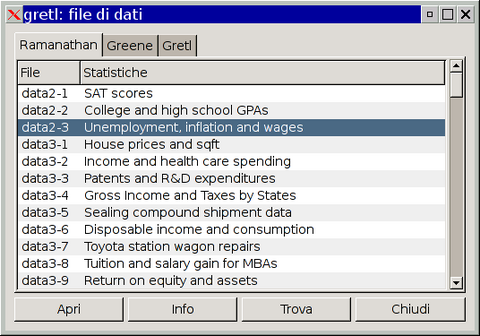
\includegraphics[scale=0.75]{figures/datafiles}
  \end{center}
  \caption{Finestra dei file di esempio}
  \label{fig-datafiles}
\end{figure}

Selezionando una riga in questa finestra e facendo clic su ``Info'',
si aprir� una finestra di descrizione del dataset in questione (che
pu� contenere informazioni a proposito della fonte dei dati e della
definizione delle variabili).  Se si trova un file interessante, �
possibile aprirlo facendo clic su ``Apri'', o semplicemente facendo
doppio clic sul nome del file. Per il momento, apriamo \verb+data3-6+.

\tip{Nelle finestre di \app{gretl} che contengono liste, facendo
  doppio clic su una riga viene eseguita l'azione predefinita per la
  relativa voce nella lista: ad esempio mostrare i valori di una
  serie, o aprire un file.} 

Questo file contiene dati relativi a un
oggetto classico dell'econometria, la funzione di consumo. La finestra
dei dati dovrebbe ora contenere il nome del file di dati in uso,
l'intervallo completo dei dati e quello del campione, i nomi delle
variabili, insieme a delle loro brevi descrizioni (si veda la Figura
\ref{fig-mainwin}).
    
\begin{figure}[htbp]
  \begin{center}
    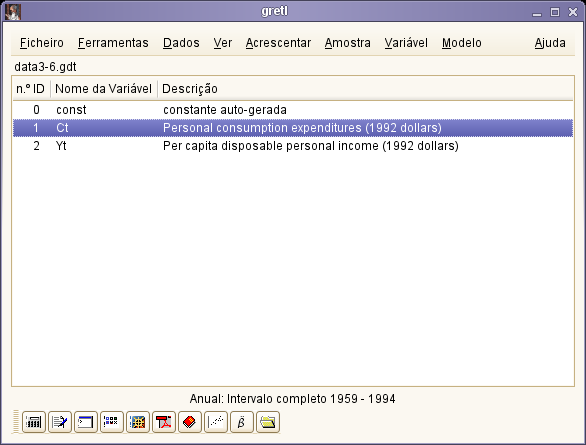
\includegraphics[scale=0.75]{figures/mainwin}
  \end{center}
  \caption{Finestra principale, con un file di esempio aperto}
  \label{fig-mainwin}
\end{figure}

OK, cosa possiamo fare ora? Le varie opzioni dei men� dovrebbero
essere abbastanza chiare: per ora ci concentreremo sul men� Modello,
ma una panoramica di tutti i men� della finestra principale � fornita
pi� avanti (si veda la sezione~\ref{menus}).
    
Il men� Modello di \app{gretl} offre varie routine di stima
econometrica: quella pi� semplice e nota � rappresentata dai minimi
quadrati ordinari (Ordinary Least Squares - OLS). Scegliendo OLS, si
apre una finestra di dialogo che richiede una \emph{specificazione del
  modello}; si veda la Figura~\ref{fig-selector}.
    
\begin{figure}[htbp]
  \begin{center}
    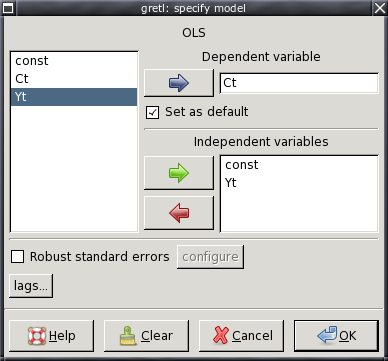
\includegraphics[scale=0.75]{figures/selector}
  \end{center}
  \caption{Specificazione del modello}
  \label{fig-selector}
\end{figure}

Per selezionare la variabile dipendente, fare clic su una variabile
nella lista di sinistra e premere il pulsante ``Scegli'' con la
freccia che punta verso il riquadro della variabile dipendente.
Selezionando la casella ``Imposta come predefinito'', la variabile
scelta verr� sempre pre-selezionata come variabile dipendente durante
le prossime aperture della finestra di dialogo.  Trucco: facendo
doppio clic su una variabile sulla sinistra, viene selezionata come
variabile dipendente e impostata come scelta predefinita.  Per
selezionare le variabili indipendenti, fare clic su di esse nella
lista di sinistra e premere il pulsante ``Aggiungi'' (o fare clic col
pulsante destro del mouse). � possibile selezionare pi� variabili
contigue trascinando il mouse; se le variabili da selezionare non sono
contigue, occorre fare clic tenendo premuto il tasto \verb+Ctrl+.  Per
eseguire una regressione con il consumo come variabile dipendente e il
reddito come variabile indipendente, fare clic su \verb+Ct+ nel
riquadro della variabile dipendente e aggiungere \verb+Yt+ alla lista
delle variabili indipendenti.

\section{Risultati della stima}
\label{est-output}


Una volta specificato un modello, apparir� una finestra che mostra i
risultati della regressione, in un formato sufficientemente chiaro e
standard (Figura~\ref{fig-modelwin}).
    
\begin{figure}[htbp]
  \begin{center}
    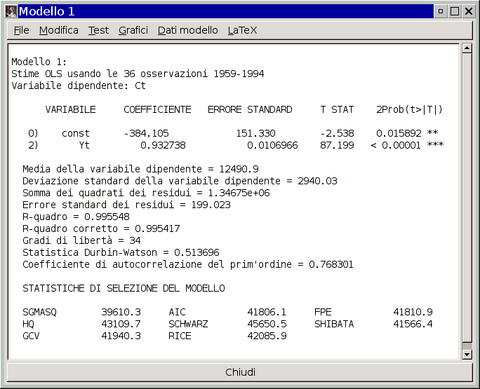
\includegraphics[scale=0.75]{figures/modelwin}
  \end{center}
  \caption{Finestra dei risultati del modello}
  \label{fig-modelwin}
\end{figure}

La finestra dei risultati contiene dei men� che consentono di
ispezionare o mostrare graficamente i residui e i valori stimati, e di
eseguire vari test diagnostici sul modello.

Per la maggior parte dei modelli c'� anche un'opzione per stampare il
risultato della regressione in formato {\LaTeX}. Si veda il
capitolo~\ref{gretltex} per i dettagli.

Per importare i risultati di \app{gretl} in un word processor, �
possibile fare copia e incolla da una finestra dei risultati usando il
men� \textsf{Modifica} (o il pulsante Copia, in alcuni contesti) nel
programma di arrivo.  Molte finestre di \app{gretl} (non tutte)
offrono l'opzione di copiare in formato RTF (il ``Rich Text Format''
di Microsoft) o come {\LaTeX}. Se si deve incollare in un word
processor, RTF pu� essere una buona opzione, visto che il formato
tabulare dei risultati viene preservato\footnote{Si noti che quando si
  copia come RTF in MS Windows, Windows permetter� di incollare il
  materiale solo in applicazioni che ``comprendono'' l'RTF. Quindi,
  sar� possibile incollare in MS Word, ma non nel Blocco Note. Inoltre
  sembra esserci un bug in alcune versioni di Windows, per cui
  l'operazione di copia non funziona se l'applicazione ``di arrivo''
  (ad es. MS Word) non � stata avviata prima di copiare il materiale
  in questione.}.  In alternativa, � possibile salvare i risultati
come file di testo semplice e importare successivamente il file nel
programma di elaborazione testi: quando si conclude una sessione di \app{gretl}
si ha l'opportunit� di salvare tutti i risultati della sessione in un unico
file.

Si noti che nel desktop \app{gnome} e in MS Windows, il men�
\textsf{File} contiene un comando per inviare i risultati direttamente
a una stampante.

\tip{Quando si incollano o si importano dei risultati di \app{gretl}
  sotto forma di testo semplice in un word processor, conviene
  selezionare un carattere a spaziatura fissa, in stile macchina da
  scrivere (ad es. il Courier), per preservare il formato tabulare dei
  risultati. Selezionare un carattere non troppo grande (Courier da 10
  punti dovrebbe andare bene) eviter� che le righe dei risultati
  vengano spezzate nei punti sbagliati.}

\section{I men� della finestra principale}
\label{menus}

Sulla barra dei men� della finestra principale si trovano, nell'ordine
da sinistra a destra, i men� File, Strumenti, Dati, Visualizza, Aggiungi,
Campione, Variabile, Modello e Aiuto.

    \begin{center}
      
\includegraphics[scale=0.75]{figures/menubar}
    \end{center}

\begin{itemize}
\item \textsf{Men� file}
  \begin{itemize}
  \item \textsf{Apri dati}: apre un file di dati in formato interno di
    \app{gretl} o lo importa da altri formati. Si veda il
    capitolo~\ref{datafiles}.
  \item \textsf{Aggiungi dati}: aggiunge dati al dataset in uso, da un
    file di dati di \app{gretl}, un file con dati separati da virgole,
    o un foglio elettronico.
  \item \textsf{Salva dati}: salva il file di dati \app{gretl} in uso.
  \item \textsf{Salva dati come}: salva il dataset in uso in formato
    interno, con la possibilit� di usare la compressione gzip. Si veda
    il capitolo~\ref{datafiles}.
  \item \textsf{Esporta dati}: salva il dataset in uso in formato CSV
    (valori separati da virgole), o nei formati di GNU R o GNU Octave.
    Si veda il capitolo~\ref{datafiles} e anche
    l'appendice~\ref{app-advanced}.
  \item \textsf{Invia a}: invia il dataset come allegato in un'e-mail.
  \item \textsf{Nuovo dataset}: permette di creare un dataset vuoto, in cui �
    possibile immettere dati manualmente o importando delle serie da un
    database. Si veda oltre per i dettagli sui database.
  \item \textsf{Abbandona dataset}: cancella dalla memoria il dataset
    in uso. Di solito questa operazione non � necessaria (visto che
    aprendo un nuovo file di dati, quello in uso viene sostituito), ma
    ci sono casi in cui � utile.
  \item \textsf{Comandi}: uno ``script'' � un file che contiene una sequenza
    di comandi di \app{gretl}. Questo men� contiene voci che permettono di
    aprire uno script di comandi creato in precedenza (``File utente''), uno
    script di esempio tra quelli forniti, o una finestra di editor per creare un
    nuovo script.
  \item \textsf{Sessioni}: un file di sessione contiene una fotografia di una
    precedente sessione di lavoro con \app{gretl}, che comprende il dataset usato
    e tutti i modelli e i grafici che sono stati salvati. Questo men� permette
    di aprire una sessione salvata in precedenza o di salvare la sessione
    in corso.
  \item \textsf{Database}: permette di consultare alcuni ampi database di serie
    storiche, disponibili sul proprio computer o, se si � connessi a internet,
    sul server dei database di \app{gretl}. Per i dettagli, si veda la sezione
    \ref{dbase}.
  \item \textsf{Funzioni}: gestisce i ``pacchetti di funzioni'' (si veda la
    sezione~\ref{sec:func-packages}), che permettono di accedere a funzioni
    scritte da altri utenti e di distribuire le proprie.
  \item \textsf{Esci}: abbandona il programma. Verr� proposto di salvare il lavoro svolto.
  \end{itemize}

\item \textsf{Men� strumenti}
  \begin{itemize}
  \item \textsf{Tavole statistiche}: cerca i valori critici per alcune
    distribuzioni di uso comune (normale o Gaussiana, \emph{t},
    chi-quadro, \emph{F} e Durbin--Watson).
  \item \textsf{Calcola p-value}: calcola i p-value per le distribuzioni
    Gaussiana, \emph{t}, chi-quadro, \emph{F}, gamma, binomiale o Poisson. Si
    veda anche il comando \cmd{pvalue} nella \GCR.
  \item \textsf{Grafici distribuzione}: produce grafici di varie distribuzioni
    di probabilit�. Il men� pop-up della finestra grafica che viene creata contiene
    il comando ``Aggiungi un'altra curva'', che permette di mostrare pi� curve
    sullo stesso grafico (ad esempio � possibile disegnare la distribuzione
    \emph{t} con vari gradi di libert�).
  \item \textsf{Calcola test}: calcola le statistiche test e i p-value
    per una serie di test di ipotesi di uso comune (media della
    popolazione, varianza e proporzione, differenza delle medie o
    delle varianze e proporzioni).
  \item \textsf{Test non parametrici}: calcola statistiche per vari test non parametrici
    (test dei segni, test di Wilcoxon, test delle successioni).
  \item \textsf{Seme per numeri casuali}: imposta il seme per il generatore di
    numeri casuali (l'impostazione predefinita si basa sull'ora di sistema in
    cui il programma � stato avviato).
  \item \textsf{Visualizza log comandi}: apre una finestra che contiene il
    registro dei comandi eseguiti fino a questo momento.
  \item \textsf{Terminale di Gretl}: apre una finestra di
    ``terminale'' in cui � possibile digitare dei comandi, come se si
    stesse usando la versione a riga di comando \app{gretlcli}, invece
    di quella con interfaccia grafica.
  \item \textsf{Avvia Gnu R}: avvia \app{R} (se � presente sul
    sistema) e vi carica una copia del dataset in uso in \app{gretl}.
    Si veda l'appendice~\ref{app-advanced}.
  \item \textsf{Ordina variabili}: riordina l'elenco delle variabili nella
    finestra principale, secondo il numero identificativo o alfabeticamente.
  \item \textsf{Test NIST}: controlla l'accuratezza numerica di
    \app{gretl} usando i test di riferimento per la regressione
    lineare adottati dal National Institute of Standards and
    Technology statunitense.
  \item \textsf{Preferenze}: imposta i percorsi per vari file a cui
    \app{gretl} ha bisogno di accedere, sceglie il carattere usato per mostrare
    i risultati, attiva o disattiva l'avviso in caso di nuove versioni
    disponibili del programma, configura la barra degli strumenti, e molte altre
    opzioni. Per ulteriori dettagli, si veda la \GCR.
  \end{itemize}

\item \textsf{Men� dati}
  \begin{itemize}
  \item \textsf{Seleziona tutto}: seleziona tutte le variabili; molti comandi
    dei men� hanno effetto sulle variabili selezionate nella finestra
    principale.
  \item \textsf{Mostra valori}: apre una finestra con un elenco (non
    modificabile) dei valori delle variabili (tutte o un sottoinsieme
    di esse).
  \item \textsf{Modifica valori}: apre una finestra di foglio
    elettronico, con cui � possibile modificare valori, aggiungere
    nuove variabili, o estendere il numero delle osservazioni.
  \item \textsf{Aggiungi osservazioni}: mostra una finestra di dialogo
    in cui � possibile scegliere un numero di osservazioni da
    aggiungere alla fine del dataset attuale; da usare per le
    previsioni.
  \item \textsf{Rimuovi osservazioni in pi�}: attivo solo se
    sono state aggiunte automaticamente delle osservazioni durante la
    procedura di previsione; cancella queste osservazioni aggiuntive.
  \item \textsf{Visualizza descrizione}, \textsf{Modifica
      descrizione}: ``Visualizza descrizione'' mostra le informazioni
    disponibili per il file di dati in uso; ``Modifica descrizione''
    permette di modificarle (se si ha il permesso di farlo).
  \item \textsf{Visualizza informazioni complete}: apre una finestra
    con una descrizione completa del dataset in uso, che include le
    informazioni di riepilogo e quelle specifiche di ogni variabile.
  \item \textsf{Aggiungi marcatori}: richiede di specificare un file
    di testo che contiene ``marcatori per le osservazioni'' (brevi
    stringhe che identificano singole osservazioni) e aggiunge queste
    informazioni al dataset. Si veda il capitolo~\ref{datafiles}.
  \item \textsf{Rimuovi marcatori}: attivo solo se il dataset contiene
    marcatori per le osservazioni; rimuove questi marcatori.
  \item \textsf{Struttura dataset}: permette di modificare
    l'interpretazione strutturale del dataset in uso. Ad esempio, se i
    dati sono stati importati come cross section, � possibile fare in
    modo che il programma li interpreti come serie storiche o come
    panel. Si veda anche la sezione~\ref{sec:data-structure}.
  \item \textsf{Compatta dati}: per serie storiche con frequenza
    superiore a quella annuale, permette di diminuire la frequenza dei
    dati, usando uno dei quattro metodi di compattamento disponibili
    (media, somma, inizio del periodo, fine del periodo).
  \item \textsf{Espandi dati}: per serie storiche, permette di aumentare la
    frequenza dei dati.
  \item \textsf{Trasponi dati}: trasforma ogni osservazione in una
    variabile e viceversa (o, in altre parole, ogni riga della matrice
    dei dati diventa una colonna della nuova matrice dei dati); pu�
    essere utile per ``raddrizzare'' dati importati in modo errato.
  \end{itemize}

\item \textsf{Men� visualizza}
  \begin{itemize}
  \item \textsf{Finestra icone}: apre una finestra che mostra la
    sessione corrente di \app{gretl} sotto forma di un insieme di
    icone. Per i dettagli si veda la sezione~\ref{session}.
  \item \textsf{Grafico}: apre una finestra di dialogo
    che permette di scegliere tra un grafico temporale, un grafico a
    dispersione X--Y, un grafico X--Y a impulsi (barre verticali), un
    grafico X--Y ``con fattore'' (ossia, con i punti colorati in modo
    diverso a seconda del valore di una data variabile dummy), un
    boxplot e un grafico 3D.  Si veda il capitolo~\ref{chap-graphs}
    per i dettagli.
  \item \textsf{Grafici multipli}: permette di comporre un insieme di
    grafici (al massimo sei) in un'unica finestra. I grafici possono essere
    a dispersione o di serie storiche.
  \item \textsf{Statistiche descrittive}: mostra un insieme abbastanza
    ricco di statistiche descrittive per tutte le variabili del
    dataset, o per le variabili selezionate.
  \item \textsf{Matrice di correlazione}: mostra i coefficienti di
    correlazione fra le variabili selezionate.
  \item \textsf{Tabulazione incrociata}: mostra una tabulazione incrociata
    fra le variabili selezionate. Occorre che almeno due variabili del dataset
    siano state marcate come discrete (si veda il Capitolo~\ref{chap:discrete}).
  \item \textsf{Componenti principali}: produce un'analisi delle componenti
    principali delle variabili selezionate.
  \item \textsf{Distanze di Mahalonobis}: calcola la distanza di
    Mahalonobis per ogni osservazione dal centroide dell'insieme di
    variabili selezionate.
  \item \textsf{Correlogramma incrociato}: calcola e mostra il correlogramma incrociato
    per due variabili selezionate.
  \end{itemize}

\item \textsf{Men� aggiungi}: offre alcune trasformazioni
  standard per le variabili (logaritmi, ritardi, quadrati, ecc) che
  � possibile aggiungere al dataset. D� anche l'opzione di
  aggiungere variabili casuali e (per i dataset di serie storiche)
  variabili dummy stagionali (ad es. variabili dummy trimestrali per
  dati trimestrali).

\item \textsf{Men� campione}
  \begin{itemize}
  \item \textsf{Imposta intervallo}: seleziona punti di partenza e
    arrivo diversi per il campione in uso, all'interno dell'intervallo
    di dati disponibili.
  \item \textsf{Ripristina campione completo}: si spiega da s�.
  \item \textsf{Imposta in base a dummy}: data una variabile dummy
    (indicatore) con valori 0 o 1, vengono scartate dal campione tutte
    le osservazioni per cui la variabile dummy vale 0.
  \item \textsf{Imposta in base a condizione}: simile al precedente,
    tranne per il fatto che non si ha bisogno di una variabile
    predefinita: basta fornire una condizione Booleana (ad es.
    \verb+sqft > 1400+) e il campione sar� ristretto alle osservazioni
    che soddisfano la condizione. Si veda la voce \cmd{genr} nella \GCR\
    per maggiori dettagli sugli operatori Booleani che possono essere
    usati.
  \item \textsf{Sotto-campione casuale}: estrae un campione casuale dal dataset.
  \item \textsf{Scarta valori mancanti}: scarta dal campione corrente
    tutte le osservazioni per cui almeno una variabile ha un valore
    mancante (si veda la sezione~\ref{missing-data}).
  \item \textsf{Conta valori mancanti}: produce un rapporto sulle
    osservazioni per cui mancano dei valori. Pu� essere utile durante
    l'esame di un dataset panel, dove � abbastanza comune incontrare
    valori mancanti.
  \item \textsf{Imposta codice valori mancanti}: imposta il valore
    numerico che sar� interpretato come ``mancante'' o ``non
    disponibile''. Questo comando � utile se si stanno utilizzando dati
    importati, per cui \app{gretl} non ha riconosciuto il codice per i valori
    mancanti.
  \end{itemize}

\item \textsf{Men� variabile}: la maggior parte di questi comandi
  opera su una sola variabile alla volta. La variabile ``attiva''
  viene impostata facendo clic sulla riga che la contiene nella
  finestra principale. La maggior parte delle opzioni si spiegano da
  sole.  Si noti che � possibile rinominare una variabile e modificare
  la sua etichetta descrittiva usando ``Modifica attributi''. � anche
  possibile definire una nuova variabile attraverso una formula (che
  pu� essere una funzione di una o pi� variabili esistenti). Per la
  sintassi di queste formule, si veda la sezione ``Definisci nuova
  variabile'' della guida in linea o la voce \cmd{genr}. Un semplice
  esempio:
          
\begin{code}
pippo = x1 * x2
\end{code}

  creer� la nuova variabile \verb+pippo+ come prodotto delle variabili
  esistenti \verb+x1+ e \verb+x2+.  In queste formule, le variabili
  devono essere indicate per nome, non per numero identificativo.

\item \textsf{Men� modello}: per i dettagli sui vari stimatori offerti
  da questo men�, si consulti la \GCR.  Si veda anche il capitolo~\ref{chap-nls}
  a proposito della stima di modelli non lineari.

\item \textsf{Men� aiuto}: usatelo!  Fornisce dettagli sulla sintassi
  dei comandi e delle finestre di dialogo.
\end{itemize}

\section{Scorciatoie da tastiera}
\label{keyb-accel}

Mentre si lavora nella finestra principale di \app{gretl}, � possibile compiere alcune
operazioni comuni utilizzando la tastiera, come mostrato nella tabella seguente:

\begin{center}
\begin{tabular}{lp{5in}}
\texttt{Invio} & Apre una finestra contenente i valori delle variabili selezionate,
  ossia, esegue il comando ``Dati, Mostra valori''.\\
\texttt{Canc} & Cancella le variabili selezionate. Per evitare cancellazioni
  accidentali � richiesta una conferma.\\
\texttt{e} & Ha lo stesso effetto del comando ``Modifica attributi'' del
  men� ``Variabile''.\\
\texttt{F2} & Ha lo stesso significato di ``e'', per compatibilit� con altri programmi.\\
\texttt{g} & Ha lo stesso effetto del comando ``Definisci nuova variabile'' dal men� ``Variabile''
  (che richiama il comando \texttt{genr}).\\
\texttt{h} & Apre la finestra di aiuto per i comandi di gretl.\\
\texttt{F1} & Ha lo stesso significato di ``h'', per compatibilit� con altri programmi.\\
\texttt{r} & Aggiorna l'elenco delle variabili nella finestra principale: ha lo
  stesso effetto del comando ``Aggiorna finestra'' nel menu ``Dati''. \\
\texttt{t} & Mostra in un grafico la variabile selezionata; per i dataset di
  tipo serie storiche viene mostrato un grafico temporale, mentre per i dati di
  tipo cross section si ottiene un grafico di distribuzione di frequenza.
\end{tabular}
\end{center}


\section{La barra degli strumenti di gretl}
\label{toolbar}

In basso a sinistra nella finestra principale si trova la barra degli
strumenti.

\begin{center}
  
\includegraphics[scale=0.75]{figures/toolbar}
\end{center}

Le icone sulla barra hanno il seguente significato, nell'ordine:

\begin{enumerate}
\item Avvia una calcolatrice. Una funzione comoda quando si ha bisogno
  di usare velocemente una calcolatrice mentre si lavora in
  \app{gretl}. Il programma avviato in modo predefinito �
  \verb+calc.exe+ in MS Windows, o \verb+xcalc+ nel sistema X window.
  � possibile cambiare il programma nel men� ``Strumenti, Preferenze,
    Generali'', sezione ``Programmi''.
\item Inizia un nuovo script. Apre una finestra in cui � possibile
  digitare una serie di comandi da eseguire in modalit� batch.
\item Apre il terminale di gretl. Una scorciatoia per il comando del
  men� ``Terminale di Gretl'' (si veda la sezione~\ref{menus}).
\item Apre la finestra delle icone di \app{gretl}.
\item Apre il sito web di \app{gretl} nel proprio browser (funziona
  solo se si � connessi a internet e si dispone di un browser).
\item Apre l'ultima versione del manuale di gretl in formato PDF.
  Richiede una connessione a internet e un browser configurato.
\item Apre questa guida in formato PDF.
\item Apre la guida in linea per la sintassi dei comandi (che mostra i
  dettagli di tutti i comandi disponibili).
\item Apre la finestra di dialogo per costruire un grafico.
\item Apre la finestra di dialogo per stimare un modello con i minimi
  quadrati ordinari.
\item Apre una finestra che elenca i dataset distribuiti insieme a \app{gretl}
  e altri dataset eventualmente installati.
\end{enumerate}

Se non si desidera visualizzare la barra degli strumenti, � possibile
disabilitarla nel men� ``Strumenti, Preferenze, Generali'',
de-selezionando la casella ``Mostra la barra degli strumenti di
gretl''.

%%% Local Variables: 
%%% mode: latex
%%% TeX-master: "gretl-guide-it"
%%% End: 


\chapter{Modalit� di lavoro}
\label{modes}

\section{Script di comandi}
\label{scripts}

I comandi \app{gretl} eseguiti utilizzando le finestre di dialogo
dell'interfaccia grafica vengono registrati sotto forma di file
``script'' o ``log''. Questi file possono essere modificati e
ri-eseguiti, usando \app{gretl} o l'applicazione a riga di comando
\app{gretlcli}.

Per visualizzare lo stato del log dei comandi durante una sessione di
\app{gretl}, basta scegliere ``Visualizza log comandi'' dal men�
``Strumenti''. Questo file di log � chiamato \verb+session.inp+ e viene
sovrascritto ogni volta che si inizia una nuova sessione: per
conservarlo, basta salvarlo con un nome diverso. I file di comandi
vengono visualizzati pi� facilmente nella finestra di selezione dei
file se vengono salvati con l'estensione ``\verb+.inp+''.

Per aprire uno script di diversa provenienza, occorre usare il comando
del men� ``File, Comandi, File utente''; per creare uno script da
zero, occorre usare ``File, Comandi, Nuovo'' dal men�, oppure
il pulsante ``Nuovo file comandi'' dalla barra degli strumenti.
In entrambi i casi si aprir� una finestra comandi (si veda la
figura~\ref{fig-scriptwin}).

\begin{figure}[htbp]
  \begin{center}
    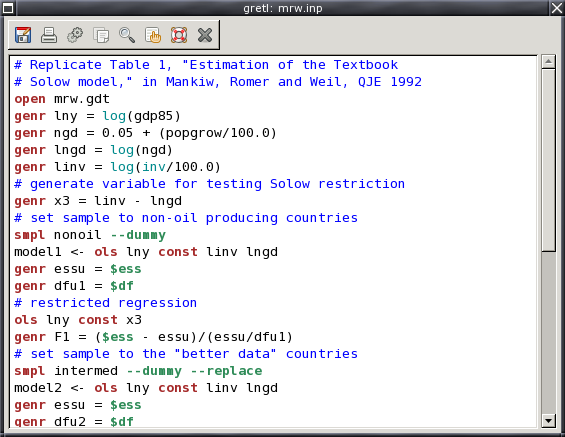
\includegraphics[scale=0.75]{figures/scriptwin}
  \end{center}
  \caption{Finestra comandi, modifica di un file di comandi}
  \label{fig-scriptwin}
\end{figure}

La barra degli strumenti in cima alla finestra comandi offre le
seguenti funzioni (da sinistra a destra): (1) Salva il file; (2) Salva
il file con un nome specifico; (3) Stampa il file (questo comando non �
disponibile su tutte le piattaforme); (4) Esegui i comandi nel file; (5) Copia il testo
selezionato; (6) Incolla il testo selezionato; (7) Cerca e sostituisci
testo; (8) Annulla l'ultimo comando Incolla o Sostituisci; (9) Aiuto
(spostando il cursore sulla parola di un comando e premendo il punto
di domanda si ottiene aiuto su quel comando); (10) Chiudi la finestra.

Quando si esegue lo script, facendo clic sull'icona ``Esegui'' o premendo
Ctrl-r, i risultati dei comandi compariranno in un'unica finestra, dove possono
essere modificati, salvati, o copiati negli appunti.  Per conoscere meglio le
possibilit� fornite dagli script, � possibile usare il comando del men� ``Aiuto,
Guida comandi'', oppure eseguire la versione a riga di comando del programma
\app{gretlcli} ed eseguire il comando ``help'', oppure ancora consultare la
\GCR.  
 
Se si esegue lo script dopo averne selezionato una parte,
\app{gretl} eseguir� solo quella parte. In pi�, se si vuole eseguire solo la
riga corrente basta premere Ctrl-Enter\footnote{Questa utile funzionalit�,
offerta anche da altri pacchetti econometrici, pu� indurre a scrivere degli
script enormi che non sono mai eseguiti interamente, ma fungono solo da archivio
per una serie di piccole porzioni di codice che vengono eseguite all'occorrenza.
Visto che \app{gretl} permette di tenere aperte molte finestre di script nello
stesso momento, � possibile mantenere i propri script ordinati in piccoli file
separati.}.

Facendo clic col tasto destro del mouse nella finestra di modifica dello script
si apre un men� pop-up, che permette di eseguire la riga su cui si trova il
cursore, oppure una regione dello script selezionata in precedenza. Se lo script
� modificabile, questo men� offre anche la possibilit� di aggiungere o rimuovere
i marcatori di commento dall'inizio della riga, o delle righe.

Il pacchetto \app{gretl} contiene pi� di 70 script ``di
esempio'': la maggior parte di essi � relativa a Ramanathan (2002),
ma essi possono essere utili anche per studiare le possibilit� di
scripting offerte da \app{gretl}, oltre ad alcuni aspetti della
teoria econometrica. � possibile esplorare i file di esempio dal men�
``File, Comandi, File di esempio'': si trover� un
elenco dei file, insieme a una breve descrizione dei problemi
illustrati nello script e dei dati utilizzati.  Basta aprire un file ed eseguirlo
per vederne i risultati.  Si noti che in uno script i comandi lunghi
possono essere suddivisi in due o pi� righe, usando una barra inversa
come carattere di continuazione della riga.

� anche possibile, se si vuole, usare insieme l'interfaccia grafica e
le funzionalit� di script, sfruttando le comodit� offerte da ognuno
dei due approcci. Ecco alcuni suggerimenti:
    
\begin{itemize}
\item Aprire un file di dati dall'interfaccia grafica, esplorare i
  dati, generare grafici, stimare regressioni, eseguire test. Quindi
  aprire il log dei comandi, rimuovere eventuali comandi ridondanti,
  salvarlo con un nome specifico ed eseguirlo, in modo da generare un
  singolo file che contiene i risultati della propria sessione di
  lavoro.
\item Partire da un nuovo file script e scrivere i comandi necessari
  per eseguire le trasformazioni desiderate su un dataset (si veda il
  comando \cmd{genr} nella \GCR). Tipicamente � possibile svolgere questo
  tipo di operazioni in modo pi� efficace scrivendo una sequenza ben
  ragionata di comandi, piuttosto che puntando e cliccando
  nell'interfaccia grafica. Salvare ed eseguire lo script: la finestra
  dei dati verr� aggiornata e sar� possibile continuare l'esplorazione
  dei dati attraverso l'interfaccia grafica. Per ripristinare lo stato
  iniziale dei dati in un secondo momento, � sufficiente aprire ed
  eseguire di nuovo lo script ``preparatorio''.
\end{itemize}

\subsection{Script e file di dati}

Un modo comune di condurre la ricerca econometrica con \app{gretl} � il
seguente: comporre uno script, eseguirlo, ispezionare i risultati, modificare lo
script, eseguirlo di nuovo, ripetendo gli ultimi tre passi per quanto �
necessario. In questo contesto, si noti che quando viene aperto un file di dati
la maggior parte delle informazioni di stato interne a \app{gretl} vengono
cancellate.  � quindi una buona idea cominciare il proprio script con un comando
\texttt{open}: in questo modo il file di dati verr� riaperto ogni volta, e si
sar� sicuri di ottenere risultati ``freschi'', non condizionati dalle esecuzioni
precedenti.

Occorre notare un punto ulteriore: quando si apre un nuovo file di dati usando
l'interfaccia grafica si viene avvertiti del fatto che aprire un nuovo file
comporta la perdita del lavoro non salvato fino a quel momento. Quando invece si
esegue uno script che apre un file di dati \textit{non} si viene avvertiti. Questo
comportamento assume che non ci sia alcun rischio di perdere lavoro fatto, visto
che il lavoro � incorporato nello script stesso (e sarebbe scomodo ricevere un
avvertimento ad ogni iterazione del ciclo di lavoro descritto sopra).

Ci� significa che occorre fare attenzione se si � eseguito del lavoro usando
l'interfaccia grafica e si vuole poi eseguire uno script: il file di dati in uso
pu� venir sostituito senza alcun avviso, ed � responsabilit� dell'utente
salvare i propri dati prima di eseguire lo script.

\section{Salvare oggetti da uno script}
\label{sect-script-objects}

Se si stima un modello usando l'interfaccia grafica, i risultati
vengono mostrati in una finestra separata, che comprende alcuni men� da cui �
possibile effettuare test, disegnare grafici, salvare dati del
modello, e cos� via. Se invece si stima un modello usando uno script,
si ottiene un tabulato non interattivo dei risultati, ma � possibile
``catturare'' i modelli stimati in uno script, in modo da esaminarli
interattivamente dopo l'esecuzione dello script. Ecco un esempio:
    
\begin{code}
Modello1 <- ols Ct 0 Yt
\end{code}

Ossia: si indica un nome con cui verr� salvato il modello,
seguito da una ``freccia di assegnazione'' rivolta all'indietro e dal
comando di stima del modello. � possibile usare spazi nei nomi dei
modelli, ma occorre racchiudere il nome tra virgolette doppie:
    
\begin{code}
"Modello 1" <- ols Ct 0 Yt
\end{code}

I modelli salvati in questo modo appariranno come icone nella finestra
delle icone di \app{gretl} (si veda la sezione~\ref{session}) dopo l'esecuzione
dello script. Inoltre, � possibile fare in modo che un modello venga mostrato in
una finestra in modo automatico, usando:
\begin{code}
Modello1.show
\end{code}

Ancora: se il nome contiene spazi, occorre metterlo tra virgolette:
\begin{code}
"Modello 1".show
\end{code}

� possibile usare la stessa procedura anche per i grafici; ad esempio,
il comando seguente crea un grafico di \verb+Ct+ rispetto a \verb+Yt+,
lo salva come ``Grafico'' (apparir� con questo nome nella finestra delle
icone) e lo mostra automaticamente:
\begin{code}
Grafico <- gnuplot Ct Yt
Grafico.show
\end{code}

� anche possibile salvare i risultati di un comando come oggetti
testuali identificati da un nome (anche questi appariranno nella
finestra della sessione, da cui sar� possibile aprirli in seguito). Ad
esempio, questo comando invia i risultati di un test Dickey--Fuller
aumentato a un ``oggetto testuale'' chiamato \verb+ADF1+ e li mostra in
una finestra:
\begin{code}
ADF1 <- adf 2 x1
ADF1.show
\end{code}

Gli oggetti salvati in questo modo (siano essi modelli, grafici o
parti di testo) possono essere eliminati usando il comando
\verb+.free+ aggiunto al nome dell'oggetto, ad esempio
\verb+ADF1.free+.

\section{Il terminale di gretl}
\label{console}

Un'altra funzionalit� comoda � contenuta nel men� ``Strumenti'' di
\app{gretl}: il ``Terminale di gretl'' (c'� anche un pulsante
``Terminale di gretl'' nella barra degli strumenti nella finestra
principale).  Si tratta di una finestra in cui � possibile scrivere
comandi ed eseguirli interattivamente uno alla volta (premendo il
tasto Invio), cos� come avviene nella versione a riga di comando
\app{gretlcli}, con la differenza che l'interfaccia grafica viene
aggiornata in base ai comandi eseguiti dal terminale, permettendo di
lavorare con entrambi gli strumenti.

Nel terminale � disponibile la ``storia dei comandi'', ossia �
possibile usare i tasti freccia su e freccia gi� per scorrere la lista
dei comandi gi� eseguiti. � possibile quindi recuperare un comando,
modificarlo ed eseguirlo di nuovo.

In modalit� terminale, � possibile creare, visualizzare e cancellare oggetti
(modelli, grafici o testo) nel modo descritto sopra per la modalit� script.

\section{Il concetto di sessione}
\label{session}

\app{gretl} offre il concetto di ``sessione'' per tenere traccia del
proprio lavoro e richiamarlo in un secondo momento. L'idea di base �
quella di fornire uno spazio che contiene, sotto forma di icone, vari
oggetti relativi alla sessione di lavoro in corso (si veda la
figura~\ref{fig-session}). � possibile aggiungere oggetti in questo
spazio e salvarli assieme alla sessione, in modo che siano disponibili
ad una successiva riapertura della sessione.
        
\begin{figure}[htbp]
  \begin{center}
    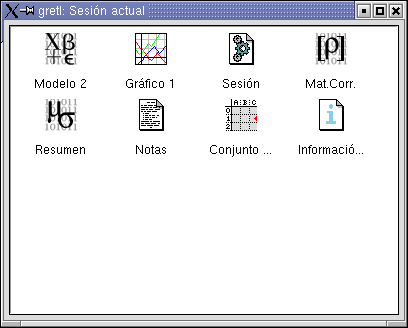
\includegraphics[scale=0.75]{figures/session}
  \end{center}
  \caption{Finestra delle icone: oltre alle icone predefinite, sono stati
    aggiunti un modello e un grafico}
  \label{fig-session}
\end{figure}

Avviando \app{gretl}, aprendo un dataset e selezionando
``Finestra icone'' dal men� ``Visualizza'', � possibile visualizzare
l'insieme predefinito di icone, che permettono di accedere rapidamente
al log dei comandi (``Comandi''), alle informazioni sul dataset
(se esistono), alla matrice di correlazione (``Correlazioni'') e
alle statistiche descrittive di riepilogo (``Statistiche'').
Tutte queste funzioni sono attivate facendo doppio clic sull'icona
relativa. L'icona ``Dataset'' � un po' pi� complessa: un doppio
clic apre i dati nel foglio di lavoro integrato, mentre facendo clic
col tasto destro del mouse si ottiene un men� con le altre azioni
possibili.

Per aggiungere un modello alla finestra delle icone, occorre per prima
cosa stimarlo usando il men� ``Modello'', quindi aprire il men� ``File'' nella
finestra del modello e selezionare ``Salva alla sessione come
  icona\dots{}'' o ``Salva come icona e chiudi''.  L'ultima
operazione pu� essere eseguita semplicemente anche premendo il tasto
\verb+S+ da dentro la finestra del modello.

Per aggiungere un grafico, occorre crearlo (dal men� ``Visualizza, Grafico'',
o attraverso uno degli altri comandi \app{gretl} di generazione dei
grafici).  Facendo clic sulla finestra del grafico si ottiene un men� da cui si
dovr� selezionare ``Salva alla sessione come icona''.

Una volta che un modello o un grafico � stato aggiunto, la sua icona
dovrebbe comparire nella finestra delle icone. Facendo
doppio clic sull'icona, l'oggetto viene visualizzato di nuovo, mentre
facendo clic con il tasto destro del mouse si ottiene un men� che
permette di visualizzare o cancellare l'oggetto, oppure di
modificarlo, se si tratta di un grafico.

\subsection{La tabella modelli}
\label{model-table}

Nella ricerca econometrica � prassi comune stimare, per una stessa
variabile dipendente, vari modelli che differiscono tra
loro per le variabili indipendenti o per lo stimatore usato.  In
questa situazione � comodo poter rappresentare i risultati delle
regressioni sotto forma di una tabella dove ogni colonna contiene i
risultati (stime dei coefficienti e errori standard) per un dato
modello e ogni riga contiene le stime per una certa variabile nei
differenti modelli.

Nella finestra delle icone, \app{gretl} d� la possibilit�
di costruire una tabella simile (e di esportarla in testo semplice,
{\LaTeX} o RTF - Rich Text Format).  Ecco come fare:\footnote{La
  tabella modelli pu� anche essere costruita in modo non interattivo
  in uno script. Per i dettagli si veda il comando \cmd{modeltab}.}
      
\begin{enumerate}
\item Stimare un modello che si vuole includere nella tabella e
  selezionare, nel men� File della finestra di visualizzazione del
  modello, ``Salva alla sessione come icona'' o ``Salva
    come icona e chiudi''.
\item Ripetere il punto 1 per gli altri modelli da includere nella
  tabella (fino a un massimo di sei modelli).
\item Completata la stima dei modelli, aprire l'icona della sessione
  di gretl, selezionando ``Finestra icone'' nel men� ``Visualizza''
  della finestra principale di gretl, o facendo clic sull'icona
  ``Finestra icone'' della barra degli strumenti di gretl.
\item La finestra delle icone contiene un'icona chiamata
  ``Tabella Modelli''. Per aggiungere alla tabella modelli il
  modello che deve apparire nella colonna pi� a sinistra della
  tabella, basta trascinare l'icona del modello sull'icona della
  Tabella Modelli, oppure fare clic col tasto destro sull'icona del
  modello e selezionare ``Aggiungi alla tabella modelli'' dal
  men� pop-up.
\item Ripetere il punto 4 per gli altri modelli da aggiungere alla
  tabella. Il secondo modello scelto apparir� nella seconda colonna da
  sinistra della tabella, e cos� via.
\item Ultimata la composizione della tabella, � possibile
  visualizzarla facendo doppio clic sulla sua icona. Per copiare la
  tabella negli appunti in uno dei formati supportati, basta fare clic
  sul men� Modifica della finestra in cui appare la tabella.
\item Se l'ordinamento dei modelli nella tabella non � quello voluto,
  fare clic col tasto destro sull'icona della tabella modelli e
  selezionare ``Pulisci'', quindi tornare al punto 4.
\end{enumerate}

Un semplice esempio di tabella modelli di \app{gretl} � mostrato nella
figura~\ref{fig-model-table}.

\begin{figure}[htbp]
  \begin{center}
    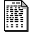
\includegraphics[scale=0.75]{figures/model_table}
  \end{center}
  \caption{Esempio della tabella modelli}
  \label{fig-model-table}
\end{figure}


\subsection{La pagina dei grafici}
\label{sect-graphpage}

L'icona ``Grafici'' della finestra delle icone offre la
possibilit� di riunire vari grafici da stampare su una sola pagina, se
si � installato il sistema di composizione {\LaTeX} e si � in grado di
generare e visualizzare file in formato PDF o postscript\footnote{Per l'output
  in PDF occorre avere il lettore Acrobat Reader di Adobe, o \app{xpdf}, se si
  usa il sistema X11. Per il postscript, occorrono \app{dvips} e \app{ghostscript},
  insieme a un visualizzatore come \app{gv}, \app{ggv} o
  \app{kghostview}. Il visualizzatore predefinito per sistemi diversi
  da MS Windows � \app{gv}.}.

Nella finestra delle icone, � possibile trascinare fino a otto
grafici sull'icona della pagina dei grafici. Facendo doppio clic
sull'icona della pagina dei grafici (o facendo clic col tasto destro e
selezionando ``Mostra''), una pagina contenente i grafici
selezionati (in formato EPS o PDF) verr� composta e aperta con il proprio
visualizzatore, da cui sar� possibile stamparla.

Per pulire la pagina dei grafici, fare clic col tasto destro
sull'icona e selezionare ``Pulisci''.

Su sistemi diversi da MS Windows, pu� essere necessario modificare
l'impostazione del programma per visualizzare il postscript,
attraverso la sezione ``Programmi'' della finestra di dialogo
delle ``Preferenze'' di gretl (nel men� ``Strumenti'' della finestra
principale).  Su Windows pu� essere necessario dover impostare le
regole di associazione dei file in modo che sia usato il
visualizzatore adeguato per l'azione ``Apri'' sui file con
estensione \verb+.ps+.

\subsection{Salvare e riaprire sessioni}
\label{session-save}

Se si creano modelli o grafici che si pensa di poter riutilizzare in
seguito, � utile selezionare ``File, Sessione, Salva come\dots{}''
prima di uscire da \app{gretl}. Per riaprire la sessione in
seguito, � possibile:

\begin{itemize}
\item Avviare \app{gretl} e riaprire il file della sessione usando il
  comando ``File, Sessione, Apri'', oppure
\item Dalla riga di comando, scrivere \cmd{gretl -r}
  \textsl{file-sessione}, dove \textsl{file-sessione} � il nome del file
  in cui � stata salvata la sessione.
\end{itemize}


%%% Local Variables: 
%%% mode: latex
%%% TeX-master: "gretl-guide-it"
%%% End: 


\chapter{File di dati}
\label{datafiles}

\section{Formato interno}
\label{native-format}

\app{gretl} utilizza un suo formato interno per i file di dati. La maggior parte
degli utenti probabilmente non � interessata a leggere o scrivere
questi file con altri programmi, ma in alcune occasioni potrebbe essere utile
farlo: per ulteriori dettagli si veda l'appendice~\ref{app-datafile}.

\section{Altri formati dei file di dati}
\label{other-formats}

\app{gretl} legge anche file di dati in altri formati:
    
\begin{itemize}
\item File di testo semplice (ASCII). Possono essere importati in
  \app{gretl} usando il comando ``File, Apri dati, Importa
  ASCII\dots{}'' dell'interfaccia grafica o il comando \cmd{import}
  dell'interfaccia a riga di comando. Per ulteriori dettagli su questo
  tipo di file, si veda la sezione~\ref{scratch}.
\item File con valori separati da virgole (CSV).  Possono essere
  importati in \app{gretl} usando il comando ``File, Apri dati,
  Importa CSV\dots{}'' dell'interfaccia grafica o il comando
  \cmd{import} dell'interfaccia a riga di comando.  Si veda anche
  la sezione~\ref{scratch}.
\item Fogli di calcolo: MS \app{Excel}, \app{Gnumeric} e Open Document
  (ODS).  Possono essere importati in \app{gretl} con il comando ``File, Apri
  dati, Importa''.  La sezione~\ref{scratch} descrive i requisiti per
  questo tipo di file.
\item File di dati di \app{Stata} (\texttt{.dta}).
\item File di lavoro di \app{Eviews} (\texttt{.wf1}).\footnote{Si veda
  \url{http://www.ecn.wfu.edu/eviews_format/}.}
\item File di dati di \app{JMulTi}.
\end{itemize}

Quando vengono importati file in formato ASCII o CSV, \app{gretl}
apre una finestra ``diagnostica'', che informa sullo stato della
lettura dei dati. Se dovessero verificarsi dei problemi a causa di
dati malformattati, questa finestra mostrer� dei suggerimenti per
risolverli.

Per venire incontro a chi vuole eseguire analisi pi� sofisticate,
\app{gretl} offre la possibilit� di salvare i dati nei formati usati
dai programmi GNU \app{R}, \app{Octave}, \app{JMulTi} e \app{PcGive} 
(si veda l'appendice~\ref{app-advanced}).  Nell'interfaccia grafica, questa
opzione si trova nel men� ``File, Esporta dati'', mentre nel client a riga di
comando occorre usare il comando \cmd{store} con l'opzione appropriata.

\section{Database binari}
\label{dbase}

Per lavorare con grandi quantit� di dati, \app{gretl} include una
routine per operare su database binari. Un \emph{database}, al
contrario di un \emph{file di dati}, non viene letto direttamente
nello spazio di lavoro del programma, ma pu� contenere serie con
frequenze e intervalli del campione diversi.  � possibile aprire un
database, selezionare delle serie e importarle nel dataset corrente;
le serie potranno poi essere salvate in un file di dati. � possibile
accedere ai database attraverso il comando ``File, Database''.

Per i dettagli sul formato dei database di \app{gretl}, si veda 
l'appendice~\ref{app-datafile}.

\subsection{Accesso ai database online}
\label{online-data}

Dalla versione 0.40, \app{gretl} � in grado di accedere ai database
via internet. Alla Wake Forest University sono disponibili alcuni
database, a cui � possibile accedere se il proprio computer � connesso
a internet. Si veda la descrizione del comando ``data'' nel men�
``Aiuto'' di \app{gretl}.

\tip{Per dettagli e aggiornamenti sui dati disponibili, basta visitare la
\href{http://gretl.sourceforge.net/gretl_data_it.html}{pagina dei dati} di
\app{gretl}.}

\subsection{Formati di database esterni}
\label{RATS}

Grazie a Thomas Doan di \emph{Estima}, che ha reso disponibili le specifiche
del formato di database usato da RATS 4 (Regression Analysis of Time
Series), \app{gretl} � in grado di gestire anche alcuni tipi di
database RATS 4: per la precisione quelli che contengono dati mensili
o trimestrali.

\app{Gretl} pu� anche importare dati dai database \app{PcGive}. Questi sono
costituiti da coppie di file, uno dei quali (con l'estensione \texttt{.bn7})
contiene i dati veri e propri, mentre quello con estensione (\texttt{.in7})
contiene informazioni supplementari.

\section{Creazione di un file di dati}
\label{scratch}

Ci sono vari modi per compiere questa operazione.

\begin{enumerate}
\item Acquisire, o creare con un editor di testo, un file di testo
  semplice ed aprirlo con il comando ``Importa ASCII'' di \app{gretl}.
\item Usare il proprio foglio di lavoro per inserire i dati, salvarlo
  in formato con valori separati da virgole (Comma Separated Values)
  se necessario (non dovrebbe essere necessario se il programma di
  foglio elettronico � MS Excel, Gnumeric o OpenOffice) e infine usare uno dei
  comandi ``Importa'' di \app{gretl}.
\item Usare il foglio elettronico contenuto in \app{gretl}.
\item Selezionare le serie di dati da un database.
\item Usare un editor di testo o altri programmi per creare un file di
  dati nel formato interno di \app{gretl}.
\end{enumerate}

Seguono alcune note a proposito dei vari metodi presentati.

\subsection{Note comuni sui dati importati}

Le opzioni 1 e 2 richiedono di usare il comando ``import'' di
\app{gretl}.  Affinch� i dati vengano letti correttamente, occorre che
siano soddisfatte alcune condizioni:

\begin{itemize}

\item La prima riga deve contenere nomi di variabile validi, ossia
  lunghi al massimo 15 caratteri (i nomi di variabile pi� lunghi
  verranno troncati a 15 caratteri), che iniziano con una lettera e
  sono composti solo da caratteri alfanumerici e dal carattere
  trattino basso, \verb+_+.  Precisazioni per i file ASCII o CSV: se
  il file non contiene righe con i nomi delle variabili, il programma
  user� automaticamente i nomi \verb+v1+, \verb+v2+ e cos� via.
  Inoltre, per ``prima riga'' si intende la prima riga
  \emph{significativa}: nel caso dei file ASCII e CSV, le righe
  bianche e quelle che iniziano con un carattere cancelletto,
  \verb+#+, vengono ignorate. Nel caso dell'importazione di file Excel
  e Gnumeric, viene presentata una finestra di dialogo in cui �
  possibile indicare il numero di righe e/o di colonne del foglio di
  lavoro da ignorare.
          
\item I valori dei dati devono costituire un blocco rettangolare, con
  una variabile per colonna e un'osservazione per riga.  Il numero
  delle varibili (colonne dei dati) deve corrispondere al numero dei
  nomi di variabile specificati.  Si veda anche la
  sezione~\ref{missing-data}. Il programma si aspetta dati di tipo
  numerico, ma nel caso di importazione da file ASCII/CSV, c'� un
  supporto limitato per dati di tipo carattere (stringa): se una
  colonna contiene solo dati di tipo stringa, le stringhe sono
  sostituite da codici numerici progressivi, e quando l'importazione
  si conclude, viene mostrata una tabella di corrispondenza tra
  stringhe e codici.
          
\item Date (o marcatori per le osservazioni): opzionalmente, la
  \emph{prima} colonna pu� contenere stringhe, come date o etichette
  identificative per osservazioni su dati cross-section. Queste
  stringhe possono essere lunghe al massimo 8 caratteri (come avviene
  per le variabili, i nomi pi� lunghi verranno troncati), mentre la
  colonna che le ospita dovrebbe avere come nome \verb+obs+ o
  \verb+date+, oppure nessun nome.

  Affinch� una stringa sia riconosciuta come data, deve rispettare uno
  dei formati seguenti: per le serie \emph{annuali}, l'anno deve
  essere indicato con quattro cifre; per le serie \emph{trimestrali}
  occorre indicare l'anno con quattro cifre, seguito da un separatore
  (punto, due punti, o la lettera \verb+Q+) e da una cifra che indica
  il trimestre, ad esempio: \verb+1997.1+, \verb+2002:3+,
  \verb+1947Q1+; per le serie \emph{mensili} occorre indicare l'anno
  con quattro cifre, seguito dal punto o dai due punti, e da due cifre
  che indicano il mese, ad esempio: \verb+1997.01+, \verb+2002:10+.
          
\end{itemize}

I file CSV possono usare virgole, spazi o tab come separatori fra le
colonne: il separatore da usare pu� essere selezionato subito dopo
aver eseguito il comando ``Importa CSV''. Se invece si usa ``Importa
ASCII'' il programma cerca di riconoscere automaticamente il
separatore usato nei dati. 

Se si usa un foglio elettronico per preparare i dati, � possibile applicare
varie trasformazioni ai dati ``grezzi'' (sommare variabili, calcolare
percentuali, ecc.), ma queste elaborazioni possono essere compiute, forse pi�
facilmente, anche in \app{gretl}, usando gli strumenti disponibili nel men�
``Aggiungi''.

\subsection{Importare dati e aggiungerli}

Pu� essere necessario costruire un dataset di \app{gretl} a poco a
poco, importando successivamente i dati da varie fonti. Questa
funzionalit� � fornita dai comandi del men� ``File, Aggiungi dati''.
\app{gretl} controller� che i nuovi dati siano compatibili con il
dataset esistente e in caso positivo aggiunger� i nuovi dati. In
questo modo � possibile aggiungere nuove variabili, a patto che la
frequenza dei dati corrisponda a quella del dataset esistente. � anche
possibile aggiungere nuove osservazioni per le serie di dati presenti
nel dataset; in questo caso i nomi delle variabili devono
corrispondere esattamente. Attenzione: se invece di ``Aggiungi dati''
si sceglie ``Apri dati'', il dataset corrente verr� chiuso.
        

\subsection{Usare il foglio elettronico interno}

� possibile creare un dataset con il comando ``File, Nuovo dataset'',
scegliendo il tipo di dati (ad es. serie storiche trimestrali, dati
cross-section), la data iniziale e quella finale (o il numero di osservazioni),
e il nome della prima variabile da creare nel dataset. Dopo aver
effettuato queste scelte, viene presentato un semplice foglio
elettronico in cui � possibile iniziare a inserire i valori. Facendo
clic col tasto destro nella finestra del foglio elettronico, comparir�
un men� che permette di aggiungere una nuova variabile (colonna), di
aggiungere una nuova osservazione (aggiungere una riga in fondo al
foglio), o di inserire un'osservazione nel punto indicato (i dati
sottostanti saranno spostati in basso e verr� inserita una riga
vuota).

Dopo aver inserito i dati nel foglio elettronico, � possibile
importarli nel foglio di lavoro di \app{gretl} premendo il pulsante
``Applica le modifiche'' nella finestra del foglio elettronico.

Si noti che il foglio elettronico di \app{gretl} � molto semplice e
non permette di inserire funzioni o formule: per trasformare i dati �
possibile usare i comandi disponibili nei men� ``Aggiungi'' o
``Variabile'' nella finestra principale di \app{gretl}.

\subsection{Estrarre dati da un database}

Un modo alternativo di creare un dataset consiste nel selezionare le
variabili da un database.

Selezionando il comando ``File, Database'', vengono presentate quattro alternative:
``Gretl'', ``RATS 4'', ``PcGive'' e ``Sul server di gretl''. Selezionando ``Gretl'', si
trover� il file \verb+fedstl.bin+, che contiene un'ampia raccolta di serie
macroeconomiche USA ed � distribuito insieme al programma.

Non si trover� nulla sotto ``RATS 4'' a meno di non aver acquistato
dei dati RATS\footnote{Si veda
  \href{http://www.estima.com/}{www.estima.com}}.  Se si possiedono
dati RATS, occorre usare il comando ``Strumenti, Preferenze, Generali...'',
selezionare la finestra Database e inserire il percorso completo dei
propri file RATS.

Se il proprio computer � connesso a internet � possibile accedere a
vari database presenti alla Wake Forest University scegliendo ``Sul server di
gretl''. � possibile consultare questi database da remoto, oppure
installarli sul proprio computer. La finestra dei database ha una
colonna che mostra, per ogni file, lo stato di installazione e lo
stato di aggiornamento della copia locale rispetto alla versione
disponibile alla Wake Forest.

Dopo aver aperto un database � anche possibile importare singole serie
nello spazio di lavoro di \app{gretl} usando il comando ``Serie, Importa''
nella finestra del database, o nel men� che compare facendo clic col
tasto destro, oppure trascinando la serie nella finestra principale
del programma.
        
\subsection{Creare un file di dati nei formati interni di gretl}

Se si hanno gi� molti dati archiviati in formato elettronico,
l'approccio migliore pu� essere quello di creare un file di dati in
uno dei formati interni di \app{gretl}, usando un editor di testo o
altri programmi come \app{awk}, \app{sed} o \app{perl}. Ovviamente
occorrer� studiare i formati di dati di \app{gretl} (il formato XML o
quello ``tradizionale'') descritti nell'appendice~\ref{app-datafile}.


\section{Struttura di un dataset}
\label{sec:data-structure}

Una volta che i dati sono stati letti da \app{gretl}, pu� essere necessario
dover fornire alcune informazioni sulla natura dei dati stessi. Distinguiamo tre
tipi di dataset:
\begin{enumerate}
\item Cross-section
\item Serie storiche
\item Dati panel
\end{enumerate}

Lo strumento principale per eseguire questa operazione � il comando del men�
``Dati, Struttura Dataset'' nell'interfaccia grafica, o il comando
\texttt{setobs} negli script e nell'interfaccia a riga di comando.

\subsection{Dati cross-section}
\label{sec:cross-section-data}

Per ``dati cross-section'' intendiamo osservazioni su una serie di ``unit�''
(che possono essere imprese, paesi, individui, ecc.) realizzate nello stesso
periodo temporale. Questa � l'interpretazione predefinita per un file di dati:
se \app{gretl} non ha informazioni sufficienti per interpretare i dati come
serie storiche o panel, essi sono automaticamente interpretati come
cross-section. Nell'improbabile caso in cui dei dati cross-section siano
interpretati come serie storiche, � possibile correggere l'errore usando il
comando del men� ``Dati, Struttura dataset'', facendo clic sul pulsante
``cross-section'', quindi su ``Avanti'', e infine su ``Ok''.

\subsection{Serie storiche}
\label{sec:timeser-data}

Quando si importano dati da un foglio elettronico o da un file di testo,
\app{gretl} cerca di estrarre tutte le informazioni temporali dalla prima
colonna dei dati. Se tuttavia la struttura di serie storiche dei dati non �
riconosciuta, � possibile usare il comando ``Dati, Struttura dataset'',
selezionare ``Serie storiche'', e successivamente selezionare la frequenza dei
dati e l'osservazione iniziale. In ogni momento � possibile fare clic su
``Indietro'' per correggere le scelte fatte.

� opportuna qualche considerazione ulteriore a proposito della frequenza dei
dati. In un dataset di serie storiche, tutte le serie devono avere la stessa
frequenza; se occorre creare un dataset combinando serie di diversa frequenza,
ad esempio mensili e trimestrali, occorre procedere nel modo seguente.

Per prima cosa occorre formulare una strategia: si desidera creare un dataset
mensile o trimestrale? Un punto da tenere in considerazione consiste nel fatto
che ``compattare'' i dati da una frequenza pi� alta (es. mensile) a una pi�
bassa (es. trimestrale) di solito non presenta problemi. Ovviamente si perde
informazione, ma in generale � accettabile, ad esempio, prendere la media di tre
osservazioni mensili per creare un'osservazione trimestrale. D'altra parte,
``espandere'' i dati da una frequenza minore a una maggiore, in generale non �
un'operazione valida.

Nella maggior parte dei casi, la strategia migliore consiste nel creare un
dataset di frequenza \textit{inferiore}, e di compattare i dati a frequenza
maggiore. Quando si importano i dati a frequenza maggiore nel dataset, il
programma propone la scelta del metodo di compattamento (media, somma, valore
all'inizio del periodo, o alla fine del periodo). Nella maggior parte dei casi,
prendere la media dei dati � una scelta appropriata.

� anche possibile importare dati di minore frequenza in un dataset a frequenza
maggiore, ma non � una scelta raccomandabile in generale.
In questi casi, \app{gretl} replica i valori della serie a frequenza minore per
quante volte � richiesto dalla nuova frequenza. Ad esempio, ipotizzando di avere
una serie trimestrale che vale 35.5 in 1990:1, il primo trimestre del 1990. Dopo
l'espansione alla frequenza mensile, il valore 35.5 verr� assegnato alle
osservazioni per i mesi di gennaio, febbraio e marzo del 1990. La variabile espansa
non sar� quindi adatta per analisi temporali ``fini'', a meno che non si abbia
buona ragione di ipotizzare che il suo valore rimanga costante nei sotto-periodi.

Una volta scelta la frequenza di un dataset, \app{gretl} offre comunque la
possibilit� di compattare o espandere tutte le serie del dataset, usando i
comandi ``Compatta dati'' ed ``Espandi dati'' del men� ``Dati'', che ovviamente
vanno eseguiti con cautela.

\subsection{Dati panel}
\label{sec:panel-data}

I dati panel possono essere visti sotto tre dimensioni, ossia le
variabili, le unit� cross-section e i periodi temporali. Ad esempio,
un particolare valore in un dataset pu� essere identificato come l'osservazione
della capitalizzazione di una certa azienda nel 1980.  Una nota terminologica:
useremo i termini ``unit� cross section'', ``unit�'' e ``gruppo'' in modo
intercambiabile per riferirci alle entit� che compongono la dimensione cross
section del panel, che potrebbero essere, ad esempio, aziende, paesi o
individui.

Per rappresentare i dati in un file testuale (e anche per poterli manipolare),
queste tre dimensioni devono in qualche modo essere riportate a due.
Questa procedura di ``appiattimento'' richiede di prendere degli
``strati'' di dati che apparterrebbero alla terza dimensione e di
impilarli nella dimensione verticale del file.

\app{Gretl} si aspetta sempre di trovare dati organizzati ``per
osservazione'', ossia in modo che ogni riga rappresenti un'osservazione
(e che ogni variabile occupi esattamente una colonna). Alla luce di
questo fatto, l'appiattimento dei dati panel pu� essere realizzato in
due modi:

\begin{itemize}
\item Pila di dati cross section: ognuno dei blocchi di dati disposti
  verticalmente contiene i valori per tutte le unit� cross-section
  in un determinato periodo.
\item Pila di serie storiche: ognuno dei blocchi di dati disposti
  verticalmente contiene serie storiche per una determinata unit�
  cross-section.
\end{itemize}

� possibile usare entrambi i metodi per inserire i dati. Internamente,
\app{gretl} usa il formato ``pila di serie storiche'' per immagazzinare i dati.

Quando si importano dati panel in \app{gretl} da un foglio di calcolo o
da un file con valori separati da virgole, la struttura panel non verr�
riconosciuta automaticamente (molto probabilmente i dati verranno
trattati come ``non datati'').  Per imporre un'interpretazione panel ai
dati, � possibile usare l'interfaccia grafica o il comando \cmd{setobs}.

Nell'interfaccia grafica, occorre usare il comando dal men� ``Campione,
Struttura dataset''. Nella prima finestra di dialogo occorre selezionare
``Panel''; in quella successiva, si hanno tre scelte. Le prime due opzioni,
``Pila di serie storiche'' e ``Pila di dati cross section'' sono utilizzabili
se il dataset � gi� organizzato in uno di questi due modi. Selezionando una di
queste due opzioni, il passo successivo � quello di indicare il numero di unit�
cross section nel dataset. La terza opzione ``Usa variabili indice'', �
utilizzabile se il dataset contiene due variabili che indicizzano le unit� e i
periodi temporali; il passo successivo prevede di indicare queste due variabili.
Ad esempio, un dataset potrebbe contenere una variabile con il codice dei paesi
osservati e una variabile che rappresenta l'anno dell'osservazione. In questo
caso, \app{gretl} riconoscer� la struttura panel dei dati a prescindere dal modo
in cui le osservazioni sono organizzate.

Il comando testuale \cmd{setobs} supporta delle opzioni che corrispondono a
quelle viste sopra nell'interfaccia grafica. Se sono disponibili delle variabili indice,
� possibile procedere nel modo seguente:
%
\begin{code}
setobs var-unita var-tempo --panel-vars
\end{code}
%
dove \texttt{var-unita} � una variabile che indicizza le unit� e 
\texttt{var-tempo} � una variabile che indicizza i periodi.
Altrimenti, � possibile usare la sintassi \verb+setobs+ \textsl{freq} \verb+1:1+
\textsl{struttura}, dove \textsl{freq} indica la ``dimensione dei blocchi'' di
dati (ossia, il numero di periodi nel caso delle pile di serie storiche, o il
numero di unit� cross section nel caso di pila di dati cross section), mentre
\textsl{struttura} pu� essere uguale a \verb+--stacked-time-series+ o
\verb+--stacked-cross-section+. Di seguito vengono mostrati due esempi: il primo
per un dataset panel sotto forma di pila di serie storiche con osservazioni per
20 periodi, il secondo per un dataset panel sotto forma di pila di dati cross
section, con 5 unit� cross section.
%
\begin{code}
setobs 20 1:1 --stacked-time-series
setobs 5 1:1 --stacked-cross-section
\end{code}

\subsubsection{Dati panel organizzati per variabile}

Talvolta i dati panel disponibili pubblicamente sono organizzati ``per variabile''.
Si supponga di avere dati per due variabili, \varname{x1} e \varname{x2},
relativi a 50 stati per 5 anni (per un totale di 250 osservazioni per
variabile). Una possibile rappresentazione testuale dei dati potrebbe iniziare
con un blocco per \varname{x1}, con 50 righe, corrispondenti agli stati e 5
colonne, corrispondenti agli anni. Seguirebbe, sotto, un blocco con una
struttura simile, relativo alla variabile \varname{x2}. Viene mostrato di seguito
un frammento di questo file di dati, con osservazioni quinquennali per il
periodo 1965--1985; occorre immaginare che la tabella continui per altri 48
stati, seguita da altre 50 righe per la variabile \varname{x2}.

\begin{center}
  \begin{tabular}{rrrrrr}
  \varname{x1} \\
     & 1965 & 1970 & 1975 & 1980 & 1985 \\
  AR & 100.0 & 110.5 & 118.7 & 131.2 & 160.4\\
  AZ & 100.0 & 104.3 & 113.8 & 120.9 & 140.6\\
  \end{tabular}
\end{center}

Se un tale file di dati viene importato in \app{gretl}\footnote{Si noti che
  occorrer� fare alcune piccole modifiche al file affinch� possa essere letto:
  bisogner� rimuovere la riga che contiene il nome della variabile (in questo
  esempio \varname{x1}) e la riga iniziale che contiene gli anni, altrimenti essi
  verranno importati come valori numerici.}, il programma
interpreter� le colonne come variabili diverse, rendendo inutilizzabili i dati.
Esiste per� un meccanismo per gestire queste situazioni, ossia la funzione
\cmd{stack} del comando \cmd{genr}.

Si consideri la prima colonna di dati nel frammento visto sopra: le prime 50
righe di questa colonna costituiscono una cross-section per la variabile
\varname{x1} nell'anno 1965. Se potessimo creare una nuova variabile sistemando
le prime 50 voci nella seconda colonna direttamente sotto le prime 50 voci della
prima colonna, staremmo costruendo un dataset disposto ``per osservazione'' (nel
primo dei due sensi definiti in precedenza: una pila di dati cross-section).
Ossia, avremmo una colonna che contiene una cross-section per \varname{x1} nel
1965, seguita da una cross-section per la stessa variabile nel 1970.

Il seguente script di gretl illustra come possiamo effettuare l'operazione, per
\varname{x1} e \varname{x2}. Assumiamo che il file di dati originale si chiami
\texttt{panel.txt} e che le colonne al suo interno siano precedute da
intestazioni con i ``nomi variabile'' \varname{p1}, \varname{p2}, \dots, \varname{p5}
(le colonne non sono vere variabili, ma per il momento ``facciamo finta'' che lo
siano).

\begin{code}
open panel.txt
genr x1 = stack(p1..p5) --length=50
genr x2 = stack(p1..p5) --offset=50 --length=50
setobs 50 1.01 --stacked-cross-section
store panel.gdt x1 x2
\end{code}

La seconda riga illustra la sintassi della funzione \cmd{stack}.
Il doppio punto nella parentesi indica un intervallo di variabili da impilare:
vogliamo impilare tutte le 5 colonne (per tutti i 5 anni). Il dataset completo
contiene 100 righe: per sistemare la variabile \varname{x1} vogliamo leggere solo
le prime 50 righe di ogni colonna: facciamo questo aggiungendo l'opzione
\verb+--length=50+. Si noti che se occorre impilare un insieme di colonne non
contigue, � possibile usare un elenco separato da virgole all'interno della
parentesi, come in

\begin{code}
genr x = stack(p1,p3,p5)
\end{code}

Nella riga 3 creiamo una pila di dati per la variabile \varname{x2}.  Ancora,
vogliamo una lunghezza (\texttt{length}) di 50 per i componenti della serie
impilata, ma questa volta vogliamo che gretl inizi a leggere dalla cinquantesima
riga dei dati originali, quindi specifichiamo \verb+--offset=50+.
La riga 4 impone un'interpretazione panel sui dati; infine, salviamo i dati in
formato gretl, con un'interpretazione panel, eliminando le ``variabili''
originali da \varname{p1} a \varname{p5}.

Lo script di esempio visto sopra � appropriato quando il numero delle variabili
da processare � piccolo. Quando ci sono molte variabili nel dataset, � pi�
efficiente usare un comando loop per costruire le nuove variabili, come mostrato
nell'esempio seguente, che ipotizza una situazione uguale a quella precedente
(50 unit�, 5 periodi) ma con 20 variabili invece che 2.

\begin{code}
open panel.txt
loop for i=1..20
  genr k = ($i - 1) * 50
  genr x$i = stack(p1..p5) --offset=k --length=50
endloop
setobs 50 1.01 --stacked-cross-section
store panel.gdt x1 x2 x3 x4 x5 x6 x7 x8 x9 x10 \
  x11 x12 x13 x14 x15 x16 x17 x18 x19 x20
\end{code}

\subsubsection{Marcatori nei dati panel}

Quando si lavora con dati panel, pu� essere utile usare dei marcatori
di facile memorizzazione per identificare le osservazioni. Per questo scopo
esiste una funzione speciale da usare con il comando \texttt{genr}.

Nell'esempio precedente, si supponga che tutti gli stati siano identificati con
codici di due lettere, presenti nella colonna pi� a sinistra del file di dati
originale. Quando si usa la funzione \cmd{stack}, questi codici verranno
impilati assieme ai valori dei dati. Se la prima riga � marcata con \texttt{AR}
per l'Arkansas, il marcatore \texttt{AR} verr� a trovarsi su ogni riga che
contiene un'osservazione relativa all'Arkansas. Tutto bene, ma questi marcatori
non danno alcuna informazione sulla data dell'osservazione. Per correggere la
situazione potremmo eseguire:

\begin{code}
genr time
genr year = 1960 + (5 * time)
genr markers = "%s:%d", marker, year
\end{code}

La prima riga genera un indice che parte da 1 e rappresenta il periodo di ogni
osservazione, mentre la seconda riga usa la variabile \texttt{time} per generare
una variabile che rappresenta l'anno dell'osservazione. La terza riga contiene
questa funzionalit� speciale: se (e solo se) il nome della nuova ``variabile''
da generare � \texttt{markers}, la parte del comando che segue il segno di
uguaglianza viene interpretata come una stringa di formattazione nello stile del
linguaggio C (andr� racchiusa tra virgolette doppie), seguita da una lista di
argomenti separati da virgola. Gli argomenti verranno stampati seguendo la
formattazione indicata e creeranno un nuovo insieme di marcatori per le
osservazioni. � possibile indicare come argomento dei nomi di variabili del
dataset, o la stringa \texttt{marker} che rappresenta il marcatore preesistente.
Gli specificatori di formato pi� utili in questo contesto sono \texttt{\%s}
per le stringhe e \texttt{\%d} per i numeri interi. Le stringhe possono essere
troncate: ad esempio \texttt{\%.3s} indica di usare solo i primi tre caratteri
della stringa. Per eliminare i caratteri iniziali da un marcatore esistente e
costruirne un altro, si pu� usare la sintassi \texttt{marker + n}, dove
\texttt{n} � un intero positivo: in questo caso, verranno omessi i primi
\texttt{n} caratteri.

Dopo aver eseguito i comandi visti sopra, i marcatori delle osservazioni
appariranno come, ad esempio, \texttt{AR:1965}, ossia, il codice a due lettere
relativo allo stato, seguito dall'anno dell'osservazione, uniti da un carattere
due punti.

\section{Valori mancanti nei dati}
\label{missing-data}

I valori mancanti vengono rappresentati internamente come
\verb+DBL_MAX+, il pi� alto numero in virgola mobile rappresentabile
sul sistema (che � probabile sia almeno 10 alla trecentesima potenza,
e non va interpretato come un valore legittimo dei dati).  Nei file di
dati in formato interno vanno rappresentati come \verb+NA+, mentre se
si importano dati in formato CSV \app{gretl} riconosce alcuni modi
comuni di rappresentare i valori mancanti: $-$999, la stringa
\verb+NA+ (in maiuscolo o minuscolo), un singolo punto, o
semplicemente una stringa vuota. Queste ultime, ovviamente, vanno
delimitate in modo opportuno, ad es. \verb+120.6,,5.38+ indica che il
valore di mezzo � mancante.

Per quanto riguarda il trattamento dei valori mancanti durante le
analisi statistiche, \app{gretl} si comporta nel modo seguente:

\begin{itemize}
\item Nel calcolo delle statistiche descrittive (media, scarto quadratico
  medio, ecc.) con il comando \cmd{summary}, i valori mancanti sono
  semplicemente ignorati, e la dimensione del campione viene corretta
  adeguatamente.
\item Nel calcolo delle regressioni, \app{gretl} per prima cosa
  corregge l'inizio e la fine del campione, troncandolo dove occorre.
  Ad esempio, possono esserci dei valori mancanti all'inizio del
  campione perch� la regressione comprende serie differenziate,
  ritardate e cos� via. Oppure i valori mancanti possono trovarsi alla
  fine del campione, a causa della compresenza di serie con diverso
  livello di aggiornamento, o di serie anticipate.
\end{itemize}

Se \app{gretl} trova dei valori mancanti ``all'interno''
dell'intervallo del campione per una regressione (che pu� anche essere
troncato), il risultato dipende dal tipo di dataset e dallo stimatore
scelto. In molti casi, il programma eseguir� le stime saltando
automaticamente le osservazioni che contengono valori mancanti,
emettendo un messaggio che indica quante osservazioni sono state
escluse. Tuttavia, ci sono procedure che non saltano automaticamente
le osservazioni mancanti: tutti gli stimatori autoregressivi, gli
stimatori di sistema (come il SUR) e i minimi quadrati non lineari.
Nel caso di dati panel, l'esclusione automatica delle osservazioni
mancanti avviene solo se il dataset risultante costituisce un panel
"bilanciato". In tutti i casi in cui l'esclusione automatica delle
osservazioni mancanti non � supportata, \app{gretl} emette un
messaggio di errore e non produce stime.  

In tutti i casi problematici dovuti a valori mancanti all'interno di
un dataset, � possibile ricorrere alla funzione \cmd{misszero} (da
usare con cautela!) del comando \cmd{genr}. Eseguendo \cmd{genr pippo
  = misszero(pluto)} � possibile produrre la serie \cmd{pippo}, che �
identica a \cmd{pluto}, tranne per il fatto che tutti i valori
mancanti sono stati trasformati in zeri. In seguito, costruendo
opportunamente delle variabili dummy, sar� possibile eliminare dalla
regressione le osservazioni che contengono valori mancanti, pur
mantenendo lo stesso intervallo del campione.\footnote{\cmd{genr}
  offre anche la funzione inversa di \cmd{misszero}, ossia
  \cmd{zeromiss}, che sostituisce in una serie i valori zero con il
  codice per i valori mancanti.}

\section{Dimensione massima dei dataset}
\label{data-limits}

La dimensione dei dataset (sia in termini di numero di variabili che di
osservazioni) � sostanzialmente limitata solo dalle caratteristiche del
computer. \app{Gretl} alloca la memoria dinamicamente e chiede al sistema
operativo tutta la memoria richiesta dai dati. Quindi un limite insuperabile
� dato dalla dimensione della memoria RAM.

Escludendo il comando OLS a precisione multipla, gretl di solito usa numeri in
virgola mobile in precisione doppia. La dimensione in byte di questi numeri
dipende dalla piattaforma, ma tipicamente � pari a otto. Per farsi un'idea delle
grandezze in gioco, ipotizzando di avere un dataset con 10.000 osservazioni su
500 variabili, si avranno 5 milioni di numeri in virgola mobile, ossia 40
milioni di byte.  Definendo il megabyte (MB) come $1024 \times 1024$ byte, come
si � soliti fare parlando di memoria RAM, la memoria occupata sar� di circa 38
MB. Il programma richiede ulteriore memoria anche per lo spazio di lavoro, ma,
anche tenendo conto di questo fatto, la gestione di un dataset di queste
dimensioni � fattibile su un PC moderno, che ha tipicamente almeno 256 MB di
RAM.

Se la RAM non pone problemi, c'� un'altra limitazione sulla dimensione dei dati,
che per� difficilmente diventa un vincolo stringente: le variabili e le
osservazioni sono indicizzate usando numeri interi col segno, che un tipico PC
memorizza come valori a 32 bit, avendo quindi un limite massimo pari a
2.147.483.647.

Questi limiti si applicano alle funzionalit� ``interne'' di \app{gretl}.
Ci sono limiti pi� stringenti per quanto riguarda due programmi esterni che sono
disponibili come aggiunte a \app{gretl} per alcuni tipi di analisi delle
serie storiche, ossia \app{TRAMO/SEATS} e \app{X-12-ARIMA}. Questi programmi
utilizzano un meccanismo di allocazione della memoria a dimensione fissa e
quindi non possono gestire serie pi� lunghe di 600 osservazioni.


\section{Raccolte di file di dati}
\label{collections}

Se si usa \app{gretl} nell'attivit� didattica, pu� essere utile creare
una raccolta di file di dati e/o di script di comandi, personalizzati
per il proprio corso, ad uso degli studenti.

A partire dalla versione 1.2.1 di \app{gretl}, ci sono tre modi per accedere a
una raccolta di file:

\begin{itemize}
\item Per i file di dati: selezionare dal men� ``File, Apri dati, File
  di esempio'', o fare clic sull'icona a forma di cartella sulla barra
  degli strumenti di \app{gretl}.
\item Per i file di comandi: selezionare dal men� ``File, Comandi, File
  di esempio''.
\end{itemize}

Quando un utente seleziona uno dei comandi visti sopra:

\begin{itemize}
\item Vengono elencati automaticamente i file di dati o di comandi
  inclusi nella distribuzione di gretl (che comprendono i file
  relativi a \emph{Introductory Econometrics} di Ramanathan e a
  \emph{Econometric Analysis} di Greene).
\item Il programma cerca alcune raccolte di dati opzionali, ad esempio
  i file relativi ad alcuni libri di testo (Davidson e MacKinnon, Gujarati,
  Stock e Watson, Verbeek, Wooldridge) e la Penn World Table (PWT 5.6). Si veda
  \href{http://gretl.sourceforge.net/gretl_data_it.html}{la pagina dei
    dati} sul sito web di gretl per ulteriori informazioni su queste
  raccolte. Se queste raccolte vengono trovate, vengono aggiunte
  all'elenco dei file disponibili.
\item Il programma infine cerca delle raccolte di dati (non
  necessariamente note) nei posti seguenti: la directory ``di
  sistema'' dei file di dati, la directory di sistema dei file di
  comandi, la directory utente e tutte le loro sotto-directory di
  primo livello. Valori tipici per i nomi di queste directory sono
  mostrati nella tabella~\ref{tab-colls}. Si noti che 
  \texttt{PERSONAL} � una parola chiave che viene espansa da Windows,
  ad esempio in ``My Documents'' se sul sistema � impostata la lingua inglese.
\end{itemize}

\begin{table}[htbp]
    \begin{center}
    \begin{tabular}{>{\raggedright\arraybackslash}p{2in}ll}
      � & \multicolumn{1}{c}{\textit{Linux}} & 
        \multicolumn{1}{c}{\textit{MS Windows}} \\
        Directory di sistema per i dati & 
        {\small \verb+/usr/share/gretl/data+} &
        {\small \verb+c:\Program Files\gretl\data+} \\
        Directory di sistema per i comandi & 
        {\small \verb+/usr/share/gretl/scripts+} &
        {\small \verb+c:\Program Files\gretl\scripts+} \\
        Directory utente &
        {\small \verb+$HOME/gretl+} &
        {\small \verb+PERSONAL\gretl+}\\
      \end{tabular}
    \end{center}
    \caption{Posizioni tipiche delle raccolte di file}
    \label{tab-colls}
  \end{table}

Le raccolte trovate verranno aggiunte all'elenco dei file
disponibili. In che formato deve essere una raccolta per essere
riconosciuta come tale? Una raccolta pu� essere costituita da un
gruppo di file di dati di \app{gretl} in formato XML (con
l'estensione \verb+.gdt+) o da un gruppo di file di comandi (con
l'estensione \verb+.inp+), in entrambi i casi accompagnati da un
``file principale'' o catalogo.  La distribuzione di \app{gretl}
contiene vari esempi di file di catalogo, ad esempio il file
\verb+descriptions+ nella sottodirectory \verb+misc+ della directory
dati di \app{gretl} e il file \verb+ps_descriptions+ nella
sottodirectory \verb+misc+ della directory dei comandi.  

Se si intende aggiungere una propria raccolta, occorrer� creare dei
file di catalogo, chiamati \verb+descriptions+ per i file di dati, e
\verb+ps_descriptions+ per i file di comandi, nelle rispettive
directory (ad es.  \url{/usr/share/gretl/data/mydata} o
\verb+c:\userdata\gretl\data\mydata+).

La sintassi dei file di catalogo (che sono file di testo) �
semplice; ecco ad esempio le prime righe del catalogo della raccolta
di file di dati ``misc'' inclusa nella distribuzione di gretl:

\begin{code}
# Gretl: various illustrative datafiles
"arma","artificial data for ARMA script example"
"ects_nls","Nonlinear least squares example"
"hamilton","Prices and exchange rate, U.S. and Italy"
\end{code}

La prima riga, che deve iniziare con un carattere cancelletto,
contiene un nome breve, qui ``Gretl'', che comparir� come etichetta
identificativa per questa raccolta nella finestra di selezione dei
dati, seguito da una virgola e da una descrizione breve della
raccolta (opzionale).

Le righe seguenti contengono due elementi, separati da una virgola e
racchiusi tra virgolette doppie. Il primo � il nome del file di dati
(escludendo l'estensione \verb+.gdt+), mentre il secondo � una breve
descrizione del contenuto del file di dati. Dovrebbe esserci una
riga come questa per ogni file di dati della raccolta.

I file di catalogo per le raccolte di file di comandi sono molto
simili a quelli appena visti, tranne per il fatto che ogni riga del
file contiene tre campi: il nome del file (senza l'estensione
\verb+.inp+), una breve descrizione del significato econometrico
della serie di comandi contenuti nel file e una breve descrizione
dei dati usati. Ecco un altro esempio: le prime righe del catalogo
della raccolta di file di comandi ``misc'' inclusa nella
distribuzione di gretl:

\begin{code}
# Gretl: various sample scripts
"arma","ARMA modeling","artificial data"
"ects_nls","Nonlinear least squares (Davidson)","artificial data"
"leverage","Influential observations","artificial data"
"longley","Multicollinearity","US employment"
\end{code}

La procedura per creare la propria raccolta di dati e renderla
disponibile agli utenti � la seguente:

\begin{enumerate}
\item Assemblare i dati, nel formato pi� comodo.
\item Convertire i dati in formato \app{gretl} e salvarli come file
  \verb+gdt+. Probabilmente il modo pi� semplice consiste
  nell'importare i dati nel programma come testo semplice, CSV o
  formato foglio elettronico (MS Excel o Gnumeric) e quindi
  salvarli. Pu� essere utile aggiungere delle descrizioni delle
  singole variabili (usando il comando ``Variabile, Modifica
  attributi'') e delle informazioni sulle fonti dei dati (usando il
  comando ``Dati, Modifica descrizione'').
\item Scrivere un file di catalogo per la raccolta, usando un editor
  di testi.
\item Copiare i file di dati e il file di catalogo in una
  sottodirectory della directory dei dati (o utente) di \app{gretl}.
\item Se la raccolta deve essere distribuita ad altri utenti, creare
  un pacchetto contenente i file di dati e il catalogo, ad esempio
  sotto forma di file zip.
\end{enumerate}

Se la raccolta creata non contiene dati proprietari, � possibile
inviarla al curatore di \app{gretl} in modo che venga resa
disponibile a tutti gli utenti del programma come pacchetto dati
opzionale.

%%% Local Variables: 
%%% mode: latex
%%% TeX-master: "gretl-guide-it"
%%% End: 


\chapter{Sub-sampling a dataset}
\label{sampling}

\section{Introduction}
\label{sample-intro}

Some subtle issues can arise here; this chapter attempts to explain
the issues.

A sub-sample may be defined in relation to a full dataset in two
different ways: we will refer to these as ``setting'' the sample and
``restricting'' the sample; these methods are discussed in
sections~\ref{sec:sample-set} and~\ref{sec:sample-restrict}
respectively. In addition section~\ref{sec:smpl-panel} discusses some
special issues relating to panel data, and
section~\ref{sec:resampling} covers resampling with replacement,
which is useful in the context of bootstrapping test statistics.

The following discussion focuses on the command-line approach. But you
can also invoke the methods outlined here via the items under the
\textsf{Sample} menu in the GUI program.


\section{Setting the sample}
\label{sec:sample-set}

By ``setting'' the sample we mean defining a sub-sample simply by
means of adjusting the starting and/or ending point of the current
sample range.  This is likely to be most relevant for time-series
data.  For example, one has quarterly data from 1960:1 to 2003:4, and
one wants to run a regression using only data from the 1970s.  A
suitable command is then

\begin{code}
smpl 1970:1 1979:4
\end{code}

Or one wishes to set aside a block of observations at the end of the
data period for out-of-sample forecasting.  In that case one might do

\begin{code}
smpl ; 2000:4
\end{code}

where the semicolon is shorthand for ``leave the starting observation
unchanged''.  (The semicolon may also be used in place of the second
parameter, to mean that the ending observation should be unchanged.)
By ``unchanged'' here, we mean unchanged relative to the last
\verb+smpl+ setting, or relative to the full dataset if no sub-sample
has been defined up to this point. For example, after

\begin{code}
smpl 1970:1 2003:4
smpl ; 2000:4
\end{code}

the sample range will be 1970:1 to 2000:4.  

An incremental or relative form of setting the sample range is also
supported.  In this case a relative offset should be given, in the
form of a signed integer (or a semicolon to indicate no change), for
both the starting and ending point. For example

\begin{code}
smpl +1 ;
\end{code}

will advance the starting observation by one while preserving the
ending observation, and

\begin{code}
smpl +2 -1
\end{code}

will both advance the starting observation by two and retard the
ending observation by one.

An important feature of ``setting'' the sample as described above is
that it necessarily results in the selection of a subset of
observations that are contiguous in the full dataset. The structure of
the dataset is therefore unaffected (for example, if it is a quarterly
time series before setting the sample, it remains a quarterly time
series afterwards).

\section{Restricting the sample}
\label{sec:sample-restrict}

By ``restricting'' the sample we mean selecting observations on the
basis of some Boolean (logical) criterion, or by means of a random
number generator.  This is likely to be most relevant for
cross-sectional or panel data.

Suppose we have data on a cross-section of individuals, recording
their gender, income and other characteristics.  We wish to select for
analysis only the women.  If we have a \verb+gender+ dummy variable
with value 1 for men and 0 for women we could do
%      
\begin{code}
smpl gender==0 --restrict
\end{code}
%
to this effect.  Or suppose we want to restrict the sample to
respondents with incomes over \$50,000.  Then we could use
%
\begin{code}
smpl income>50000 --restrict
\end{code}

A question arises: if we issue the two commands above in sequence,
what do we end up with in our sub-sample: all cases with income over
50000, or just women with income over 50000? By default, the answer is
the latter: women with income over 50000.  The second restriction
augments the first, or in other words the final restriction is the
logical product of the new restriction and any restriction that is
already in place.  If you want a new restriction to replace any
existing restrictions you can first recreate the full dataset using
%
\begin{code}
smpl --full
\end{code}
%
Alternatively, you can add the \verb+replace+ option to the
\verb+smpl+ command:
%
\begin{code}
smpl income>50000 --restrict --replace
\end{code}

This option has the effect of automatically re-establishing the full
dataset before applying the new restriction.

Unlike a simple ``setting'' of the sample, ``restricting'' the sample
may result in selection of non-contiguous observations from the full
data set.  It may therefore change the structure of the data set.

This can be seen in the case of panel data.  Say we have a panel of
five firms (indexed by the variable \verb+firm+) observed in each of
several years (identified by the variable \verb+year+).  Then the
restriction
%
\begin{code}
smpl year==1995 --restrict
\end{code}
%
produces a dataset that is not a panel, but a cross-section for the
year 1995.  Similarly
%
\begin{code}
smpl firm==3 --restrict
\end{code}
%
produces a time-series dataset for firm number 3.

For these reasons (possible non-contiguity in the observations,
possible change in the structure of the data), gretl acts differently
when you ``restrict'' the sample as opposed to simply ``setting'' it.
In the case of setting, the program merely records the starting and
ending observations and uses these as parameters to the various
commands calling for the estimation of models, the computation of
statistics, and so on. In the case of restriction, the program makes a
reduced copy of the dataset and by default treats this reduced copy as
a simple, undated cross-section---but see the further discussion of
panel data in section~\ref{sec:smpl-panel}.

If you wish to re-impose a time-series interpretation of the reduced
dataset you can do so using the \cmd{setobs} command, or the GUI menu
item ``Data, Dataset structure''.

The fact that ``restricting'' the sample results in the creation of a
reduced copy of the original dataset may raise an issue when the
dataset is very large.  With such a dataset in memory, the creation of
a copy may lead to a situation where the computer runs low on memory
for calculating regression results.  You can work around this as
follows:

\begin{enumerate}
\item Open the full data set, and impose the sample restriction.
\item Save a copy of the reduced data set to disk.
\item Close the full dataset and open the reduced one.
\item Proceed with your analysis.
\end{enumerate}

\subsection{Random sub-sampling}
\label{sample-random}

Besides restricting the sample on some deterministic criterion, it may
sometimes be useful (when working with very large datasets, or perhaps
to study the properties of an estimator) to draw a random sub-sample
from the full dataset.  This can be done using, for example,
%
\begin{code}
smpl 100 --random
\end{code}
%
to select 100 cases.  If you want the sample to be reproducible, you
should set the seed for the random number generator first, using the
\cmd{set} command.  This sort of sampling falls under the
``restriction'' category: a reduced copy of the dataset is made.

\section{Panel data}
\label{sec:smpl-panel}

Consider for concreteness the Arellano--Bond dataset supplied with
gretl (\texttt{abdata.gdt}). This comprises data on 140 firms
$(n=140$) observed over the years 1976--1984 $(T=9)$. The dataset is
``nominally balanced'' in the sense that that the time-series length
is the same for all countries (this being a requirement for a dataset
to count as a panel in gretl), but in fact there are many missing
values (\texttt{NA}s).

You may want to sub-sample such a dataset in either the
cross-sectional dimension (limit the sample to a subset of firms) or
the time dimension (e.g.\ use data from the 1980s only). The simplest
(but limited) way to sub-sample on firms keys off the notation used by
gretl for panel observations. The full data range is printed as
\texttt{1:1} (firm 1, period 1) to \texttt{140:9} (firm 140, period
9). The effect of
%
\begin{code}
smpl 1:1 80:9
\end{code}
%
is to limit the sample to the first 80 firms. Note that if you instead
tried \texttt{smpl 1:1 80:4}, gretl would insist on preserving the
balance of the panel and would truncate the range to ``complete''
firms, as if you had typed \texttt{smpl 1:1 79:9}.

The firms in the Arellano--Bond dataset are anonymous, but suppose you
had a panel with five named countries. With such a panel you can
inform gretl of the names of the groups using the \cmd{setobs}
command. For example, given
%
\begin{code}
string cstr = "Portugal Italy Ireland Greece Spain"
setobs country cstr --panel-groups 
\end{code}
%
gretl creates a string-valued series named \texttt{country} with group
names taken from the variable \texttt{cstr}. Then, to include only
Italy and Spain you could do
%
\begin{code}
smpl country=="Italy" || country=="Spain" --restrict
\end{code}
%
or to exclude one country,
%
\begin{code}
smpl country!="Ireland" --restrict
\end{code}

To sub-sample in the time dimension, use of \option{restrict} is
required. For example, the Arellano--Bond dataset contains a variable
named \texttt{YEAR} that records the year of the observations and if
one wanted to omit the first two years of data one could do
%
\begin{code}
smpl YEAR >= 1978 --restrict
\end{code}
%
If a dataset does not already incude a suitable variable for this
purpose one can use the command \texttt{genr time} to create a simple
1-based time index.

Note that if you apply a sample restriction that just selects certain
units (firms, countries or whatever), or selects certain contiguous
time-periods---such that $n>1$, $T>1$ and the time-series length is
still the same across all included units---your sub-sample will still
be interpreted by gretl as a panel.


\subsection{Unbalancing restrictions}

In some cases one wants to sub-sample according to a criterion that
``cuts across the grain'' of a panel dataset. For instance, suppose you
have a micro dataset with thousands of individuals observed over
several years and you want to restrict the sample to observations on
employed women.  

If we simply extracted from the total $nT$ rows of the dataset those
that pertain to women who were employed at time $t$ $(t = 1,\dots,T)$
we would likely end up with a dataset that doesn't count as a panel in
gretl (because the specific time-series length, $T_i$, would differ
across individuals). In some contexts it might be OK that gretl
doesn't take your sub-sample to be a panel, but if you want to apply
panel-specific methods this is a problem. You can solve it by giving
the \option{balanced} option with \cmd{smpl}. For example, supposing
your dataset contained dummy variables \texttt{gender} (with the value
1 coding for women) and \texttt{employed}, you could do
%
\begin{code}
smpl gender==1 && employed==1 --restrict --balanced
\end{code}
%
What exactly does this do? Well, let's say the years of your data are
2000, 2005 and 2010, and that some women were employed in all of those
years, giving a maximum $T_i$ value of 3. But individual 526 is a
women who was employed only in the year 2000 ($T_i = 1$). The effect
of the \option{balanced} option is then to insert ``padding rows'' of
\texttt{NA}s for the years 2005 and 2010 for individual 526, and
similarly for all individuals with $0 < T_i < 3$. Your sub-sample
then qualifies as a panel.


\section{Resampling and bootstrapping}
\label{sec:resampling}

Given an original data series \varname{x}, the command
%
\begin{code}
series xr = resample(x)
\end{code}
%
creates a new series each of whose elements is drawn at random from
the elements of \varname{x}.  If the original series has 100
observations, each element of \varname{x} is selected with probability
$1/100$ at each drawing.  Thus the effect is to ``shuffle'' the
elements of \varname{x}, with the twist that each element of
\varname{x} may appear more than once, or not at all, in \varname{xr}.

The primary use of this function is in the construction of bootstrap
confidence intervals or p-values.  Here is a simple example.  Suppose
we estimate a simple regression of $y$ on $x$ via OLS and find that
the slope coefficient has a reported $t$-ratio of 2.5 with 40 degrees
of freedom.  The two-tailed p-value for the null hypothesis that the
slope parameter equals zero is then 0.0166, using the $t(40)$
distribution.  Depending on the context, however, we may doubt whether
the ratio of coefficient to standard error truly follows the $t(40)$
distribution.  In that case we could derive a bootstrap p-value as
shown in Example~\ref{resampling-loop}.  

Under the null hypothesis that the slope with respect to $x$ is zero,
$y$ is simply equal to its mean plus an error term.  We simulate $y$
by resampling the residuals from the initial OLS and re-estimate the
model.  We repeat this procedure a large number of times, and record
the number of cases where the absolute value of the $t$-ratio is
greater than 2.5: the proportion of such cases is our bootstrap
p-value.  For a good discussion of simulation-based tests and
bootstrapping, see Davidson and MacKinnon
(\citeyear{davidson-mackinnon04}, chapter 4); Davidson and Flachaire
(\citeyear{davidson-flachaire01}) is also instructive.

\begin{script}[htbp]
  \caption{Calculation of bootstrap p-value}
  \label{resampling-loop}
\begin{scode}
ols y 0 x
# save the residuals
genr ui = $uhat
scalar ybar = mean(y)
# number of replications for bootstrap
scalar replics = 10000
scalar tcount = 0
series ysim
loop replics --quiet
  # generate simulated y by resampling
  ysim = ybar + resample(ui)
  ols ysim 0 x
  scalar tsim = abs($coeff(x) / $stderr(x))
  tcount += (tsim > 2.5)
endloop      
printf "proportion of cases with |t| > 2.5 = %g\n", tcount / replics
\end{scode}
%$
\end{script}

    
%%% Local Variables: 
%%% mode: latex
%%% TeX-master: "gretl-guide"
%%% End: 


\chapter{Graphs and plots}
\label{chap-graphs}

\section{Gnuplot graphs}
\label{gnuplot-graphs}

A separate program, \app{gnuplot}, is called to generate graphs.
Gnuplot is a very full-featured graphing program with myriad options.
It is available from \href{http://www.gnuplot.info/}{www.gnuplot.info}
(but note that a suitable copy of gnuplot is bundled with the packaged
versions of gretl for MS Windows and Mac OS X).  Gretl gives you
direct access, via a graphical interface, to a subset of gnuplot's
options and it tries to choose sensible values for you; it also allows
you to take complete control over graph details if you wish.

With a graph displayed, you can click on the graph window for a pop-up
menu with the following options.

\begin{itemize}
\item \textsf{Save as PNG}: Save the graph in Portable Network
  Graphics format (the same format that you see on screen).
\item \textsf{Save as postscript}: Save in encapsulated postscript
  (EPS) format.
\item \textsf{Save as Windows metafile}: Save in Enhanced Metafile
  (EMF) format.
\item \textsf{Save to session as icon}: The graph will appear in
  iconic form when you select ``Icon view'' from the View menu.
\item \textsf{Zoom}: Lets you select an area within the graph for
  closer inspection (not available for all graphs).
\item \textsf{Print}: (Current GTK or MS Windows only) lets you
  print the graph directly.
\item \textsf{Copy to clipboard}: MS Windows only, lets you paste the
  graph into Windows applications such as MS Word.
\item \textsf{Edit}: Opens a controller for the plot which lets you
  adjust many aspects of its appearance.
\item \textsf{Close}: Closes the graph window.
\end{itemize}


\subsection{Displaying data labels}
\label{plot-labels}

For simple X-Y scatter plots, some further options are available if
the dataset includes ``case markers'' (that is, labels identifying
each observation).\footnote{For an example of such a dataset, see the
  Ramanathan file \verb+data4-10+: this contains data on private
  school enrollment for the 50 states of the USA plus Washington, DC;
  the case markers are the two-letter codes for the states.} With a
scatter plot displayed, when you move the mouse pointer over a data
point its label is shown on the graph.  By default these labels are
transient: they do not appear in the printed or copied version of the
graph.  They can be removed by selecting ``Clear data labels'' from
the graph pop-up menu. If you want the labels to be affixed
permanently (so they will show up when the graph is printed or
copied), select the option ``Freeze data labels'' from the pop-up
menu; ``Clear data labels'' cancels this operation.  The other
label-related option, ``All data labels'', requests that case markers
be shown for all observations.  At present the display of case markers
is disabled for graphs containing more than 250 data points.


\subsection{GUI plot editor}
\label{plot-editor}

Selecting the \textsf{Edit} option in the graph popup menu opens
an editing dialog box, shown in Figure~\ref{fig-plot}.  Notice that
there are several tabs, allowing you to adjust many aspects of
a graph's appearance: font, title, axis scaling, line colors
and types, and so on.  You can also add lines or descriptive
labels to a graph (under the Lines and Labels tabs).  The
``Apply'' button applies your changes without closing the
editor; ``OK'' applies the changes and closes the dialog.

\begin{figure}[htbp]
  \begin{center}
    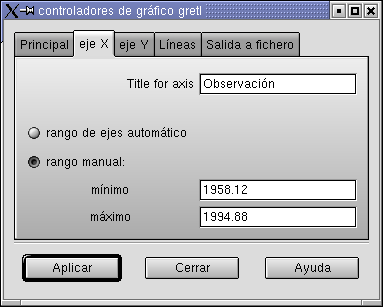
\includegraphics[scale=0.6]{figures/plot_control}
  \end{center}
  \caption{gretl's gnuplot controller}
  \label{fig-plot}
\end{figure}


\subsection{Publication-quality graphics: advanced options}
\label{plot-advanced}

The GUI plot editor has two limitations.  First, it cannot represent
all the myriad options that \app{gnuplot} offers. Users who are
sufficiently familiar with \app{gnuplot} to know what they're missing
in the plot editor presumably don't need much help from gretl,
so long as they can get hold of the \app{gnuplot} command file that
gretl has put together.  Second, even if the plot editor meets
your needs, in terms of fine-tuning the graph you see on screen, a few
details may need further work in order to get optimal results for
publication.

Either way, the first step in advanced tweaking of a graph is to get
access to the graph command file.

\begin{itemize}
\item In the graph display window, right-click and choose ``Save to
  session as icon''.
\item If it's not already open, open the icon view window---either
  via the menu item View/Icon view, or by clicking the ``session icon
  view'' button on the main-window toolbar.
\item Right-click on the icon representing the newly added graph and
  select ``Edit plot commands'' from the pop-up menu.
\item You get a window displaying the plot file
  (Figure~\ref{fig:plot-edit}).
\end{itemize}

\begin{figure}[htbp]
  \centering
  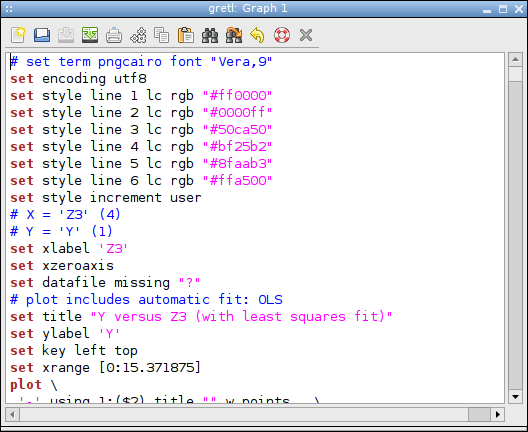
\includegraphics[scale=0.6]{figures/plotedit}
  \caption{Plot commands editor}
  \label{fig:plot-edit}
\end{figure}

Here are the basic things you can do in this window.  Obviously, you
can edit the file you just opened.  You can also send it for
processing by gnuplot, by clicking the ``Execute'' (cogwheel)
icon in the toolbar.  Or you can use the ``Save as'' button to save
a copy for editing and processing as you wish.

Unless you're a gnuplot expert, most likely you'll only need to edit a
couple of lines at the top of the file, specifying a driver (plus
options) and an output file.  We offer here a brief summary of some
points that may be useful.

First, \app{gnuplot}'s output mode is set via the command \texttt{set
  term} followed by the name of a supported driver (``terminal'' in
gnuplot parlance) plus various possible options.  (The top line in the
plot commands window shows the \texttt{set term} line that gretl
used to make a PNG file, commented out.)  The graphic formats that are
most suitable for publication are PDF and EPS.  These are supported by
the gnuplot \texttt{term} types \texttt{pdf}, \texttt{pdfcairo} and
\texttt{postscript} (with the \texttt{eps} option).  The
\texttt{pdfcairo} driver has the virtue that is behaves in a very
similar manner to the PNG one, the output of which you see on screen.
This is provided by the version of gnuplot that is included in the
gretl packages for MS Windows and Mac OS X; if you're on Linux
it may or may be supported.  If \texttt{pdfcairo} is not available,
the \texttt{pdf} terminal may be available; the \texttt{postscript}
terminal is almost certainly available.

Besides selecting a term type, if you want to get gnuplot to write the
actual output file you need to append a \texttt{set output} line
giving a filename.  Here are a few examples of the first two lines you
might type in the window editing your plot commands.  We'll make
these more ``realistic'' shortly.
%
\begin{code}
set term pdfcairo
set output 'mygraph.pdf'

set term pdf
set output 'mygraph.pdf'

set term postscript eps
set output 'mygraph.eps'
\end{code}

There are a couple of things worth remarking here.  First, you may
want to adjust the size of the graph, and second you may want to
change the font.  The default sizes produced by the above drivers are
5 inches by 3 inches for \texttt{pdfcairo} and \texttt{pdf}, and 5
inches by 3.5 inches for \texttt{postscript eps}.  In each case
you can change this by giving a size specification, which takes the
form \texttt{XX,YY} (examples below).  

You may ask, why bother changing the size in the gnuplot command file?
After all, PDF and EPS are both vector formats, so the graphs can be
scaled at will.  True, but a uniform scaling will also affect the font
size, which may end looking wrong.  You can get optimal results by
experimenting with the \texttt{font} and \texttt{size} options to
\app{gnuplot}'s \texttt{set term} command.  Here are some examples
(comments follow below).
%
\begin{code}
# pdfcairo, regular size, slightly amended
set term pdfcairo font "Sans,6" size 5in,3.5in
# or small size
set term pdfcairo font "Sans,5" size 3in,2in

# pdf, regular size, slightly amended
set term pdf font "Helvetica,8" size 5in,3.5in
# or small
set term pdf font "Helvetica,6" size 3in,2in

# postscript, regular 
set term post eps solid font "Helvetica,16"
# or small
set term post eps solid font "Helvetica,12" size 3in,2in
\end{code}

On the first line we set a sans serif font for \texttt{pdfcairo} at a
suitable size for a 5 $\times$ 3.5 inch plot (which you may find looks
better than the rather ``letterboxy'' default of 5 $\times$ 3).  And
on the second we illustrate what you might do to get a smaller 3
$\times$ 2 inch plot. You can specify the plot size in centimeters
if you prefer, as in
\begin{code}
set term pdfcairo font "Sans,6" size 6cm,4cm
\end{code}

We then repeat the exercise for the \texttt{pdf} terminal.  Notice
that here we're specifying one of the 35 standard PostScript fonts,
namely Helvetica.  Unlike \texttt{pdfcairo}, the plain \texttt{pdf}
driver is unlikely to be able to find fonts other than these.

In the third pair of lines we illustrate options for the
\texttt{postscript} driver (which, as you see, can be abbreviated as
\texttt{post}).  Note that here we have added the option
\texttt{solid}.  Unlike most other drivers, this one uses dashed lines
unless you specify the \texttt{solid} option.  Also note that we've
(apparently) specified a much larger font in this case.  That's
because the \texttt{eps} option in effect tells the
\texttt{postscript} driver to work at half-size (among other things),
so we need to double the font size.

Table~\ref{tab:drivers} summarizes the basics for the three drivers we
have mentioned.

\begin{table}[htbp]
  \centering
  \begin{tabular}{lcc}
    Terminal & default size (inches) & suggested font \\ [6pt]
    \texttt{pdfcairo} & 5 $\times$ 3 &   Sans,6 \\
    \texttt{pdf}      & 5 $\times$ 3 &   Helvetica,8 \\
    \texttt{post eps} & 5 $\times$ 3.5 & Helvetica,16 \\
  \end{tabular}
  \caption{Drivers for publication-quality graphics}
  \label{tab:drivers}
\end{table}

To find out more about \app{gnuplot} visit
\href{http://www.gnuplot.info/}{www.gnuplot.info}. This site has
documentation for the current version of the program in various
formats.

\subsection{Additional tips}
\label{subsect-graph-tips}

To be written.  Line widths, enhanced text.  Show a ``before and
after'' example.  

\section{Plotting graphs from scripts}
\label{sec:plotenv}

When working with scripts, you may want to have a graph shown onto
your display or saved into a file. In fact, if in your usual workflow
you find yourself creating similar graphs over and over again, you
might want to consider the option of writing a script which automates
this process for you. \app{Gretl} gives you two main tools for doing
this: one is a command called \cmd{gnuplot}, whose main use is to
create standard plot quickly. The other one is the \cmd{plot} command
block, which has a more elaborate syntax but offers you more control
on output.

\subsection{The \cmd{gnuplot} command}
\label{sec:gnuplot-cmd}

The \cmd{gnuplot} command is described at length in the \GCR\ and the
online help system. Here, we just summarize its main features:
basically, it consists of the \cmd{gnuplot} keyword, followed by a
list of items, telling the command \emph{what} you want plotted and a
list of options, telling it \emph{how} you want it plotted.

For example, the line
\begin{code}
gnuplot y1 y2 x   
\end{code}
will give you a basic XY plot of the two series \texttt{y1} and
\texttt{y2} on the vertical axis versus the series \texttt{x} on the
horizontal axis. In general, the arguments to the \cmd{gnuplot}
command is a list of series, the last of which goes on the x-axis,
while all the other ones go onto the y-axis. By default, the
\cmd{gnuplot} command gives you a scatterplot. If you just have one
variable on the y-axis, then \app{gretl} will also draw a the OLS
interpolation, if the fit is good enough.\footnote{The technical
  condition for this is that the two-tailed $p$-value for the slope
  coefficient should be under 10\%.}

Several aspects of the behavior described above can be modified. You
do this by appending options to the command. Most options can be
broadly grouped in three categories:
\begin{enumerate}
\item Plot styles: we support points (the default choice), lines,
  lines and points together, and impulses (vertical lines). 
\item Algorithm for the fitted line: here you can choose between
  linear, quadratic and cubic interpolation, but also more exotic
  choices, such as semi-log, inverse or loess (non-parametric). Of
  course, you can also turn this feature off.
\item Input and output: you can choose whether you want your graph on
  your computer screen (and possibly use the in-built graphical widget
  to further customize it --- see above, page \pageref{plot-editor}),
  or rather save it to a file. We support several graphical formats,
  among which PNG and PDF, to make it easy to incorporate your
  plots into text documents.
\end{enumerate}

The following script uses the AWM dataset to exemplify some
traditional plots in macroeconomics:

\begin{scode}
open AWM.gdt --quiet

# --- consumption and income, different styles ------------

gnuplot PCR YER
gnuplot PCR YER --output=display
gnuplot PCR YER --output=display --time-series
gnuplot PCR YER --output=display --time-series --with-lines

# --- Phillips' curve, different fitted lines -------------

gnuplot INFQ URX --output=display
gnuplot INFQ URX --suppress-fitted --output=display
gnuplot INFQ URX --inverse-fit --output=display
gnuplot INFQ URX --loess-fit --output=display
\end{scode}

FIXME: comment on the above

For more detail, consult the \GCR.


\subsection{The \cmd{plot} command block}
\label{sec:plotblock}

The \cmd{plot} environment is a way to pass information to
\app{Gnuplot} in a more structured way, so that customization of basic
plots becomes easier. It has the following characteristics:

The block starts with the \cmd{plot} keyword, followed by a required
parameter: the name of a list, a single series or a matrix. This
parameter specifies the data to be plotted. The starting line may be
prefixed with the \verb|savename <-| apparatus to save a plot as an icon
in the GUI program. The block ends with \cmd{end plot}.

Inside the block you have zero or more lines of these types, identified 
by an initial keyword:
\begin{description}
\item[\normalfont \texttt{option}:] specify a single option (details below)
\item[\normalfont \texttt{options}:] specify multiple options on a single line; if
  more than one option is given on a line, the options should be
  separated by spaces.
\item[\normalfont \texttt{literal}:] a command to be passed to gnuplot literally 
\item[\normalfont \texttt{printf}:] a printf statement whose result will be passed
  to gnuplot literally; this allows the use of string variables
  without having to resort to \verb!@!-style string substitution.
\end{description}

The options available are basically those of the current \cmd{gnuplot} 
command, but with a few differences. For one thing you don't need the 
leading double-dash in an "option" (or "options") line. Besides that,
\begin{itemize}
\item You can't use the option \option{matrix=whatever} with \cmd{plot}:
  that possibility is handled by providing the name of a matrix on the
  initial \cmd{plot} line.
\item The \option{input=filename} option is not supported: use
  \cmd{gnuplot} for the case where you're supplying the entire plot
  specification yourself.
\item The several options pertaining to the presence and type of a
  fitted line, are replaced in \cmd{plot} by a single option \cmd{fit} which
  requires a parameter. Supported values for the parameter are: none,
  linear, quadratic, cubic, inverse, semilog and loess. Example:
\begin{code}
  option fit=quadratic
\end{code}
\end{itemize}

As with \cmd{gnuplot}, the default is to show a linear fit in an X-Y
scatter if it's significant at the 10 percent level.

Here's a simple example, the plot spec from the "bandplot" package,
which shows how to achieve the same result via the \cmd{command} and
the \cmd{plot} block, respectively:

\begin{code}
   gnuplot 1 2 3 4 --with-lines --matrix=plotmat \
   --suppress-fitted --output=display \
   { set linetype 3 lc rgb "#0000ff"; set title "@title"; \
     set nokey; set xlabel "@xname"; }
\end{code}

\begin{code}
   plot plotmat
     options with-lines fit=none
     literal set linetype 3 lc rgb "#0000ff"
     literal set nokey
     printf "set title \"%s\"", title
     printf "set xlabel \"%s\"", xname
   end plot --output=display
\end{code}

Note that \option{output=display} is appended to \cmd{end plot}; also
note that if you give a matrix to \cmd{plot} it's assumed you want to
plot all the columns. In addition, if you give a single series and the
dataset is time series, it's assumed you want a time-series plot.

FIXME: provide an example with real data.

\section{Boxplots}
\label{sect-boxplots}

\begin{figure}[htbp]
  \begin{center}
    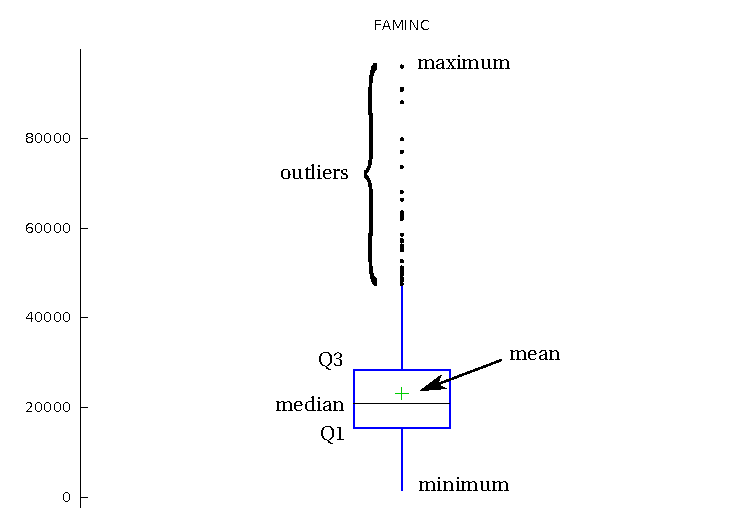
\includegraphics{figures/boxplot_sample}
  \end{center}
  \caption{Sample boxplot}
  \label{fig-boxplot}
\end{figure}

These plots (after Tukey and Chambers) display the distribution of a
variable. The central box encloses the middle 50 percent of the data,
i.e.\ it is bounded by the first and third quartiles.  The
``whiskers'' extend to from each end of the box for a range equal to
1.5 times the interquartile range. Observations outside that range are
considered outliers and represented via dots.\footnote{To give you an
  intuitive idea, if a variable is normally distributed, the chances
  of picking an outlier by this definition are slightly below 0.7\%.}
A line is drawn across the box at the median and a ``\texttt{+}'' sign
identifies the mean---see Figure~\ref{fig-boxplot}.

In the case of boxplots with confidence intervals, dotted lines show
the limits of an approximate 90 percent confidence interval for the
median.  This is obtained by the bootstrap method, which can take a
while if the data series is very long. For details on constructing
boxplots, see the entry for \cmd{boxplot} in the \GCR\, or use the
\textsf{Help} button that appears when you select one of the boxplot
items under the menu item ``View, Graph specified vars'' in the main
gretl window.

\subsection{Factorized boxplots}

A nice feature which is quite useful for data visualization is the
conditional, or factorized boxplot.  This type of plot allows you to
examine the distribution of a variable conditional on the value of
some discrete factor.

As an example, we'll use one of the datasets supplied with
\app{gretl}, that is \cmd{rac3d}, which contains an example taken from
\cite{cameron-trivedi13} on the health conditions of 5190 people. The
script below compares the unconditional (marginal) distribution of the
number of illnesses in the past 2 weeks with the distribution of the
same variable, conditional on age classes.

\begin{scode}
open rac3d.gdt
# unconditional boxplot
boxplot ILLNESS --output=display
# create a discrete variable for age class: 
# 0 = below 20, 1 = between 20 and 39, etc
series age_class = floor(AGE/0.2)
# conditional boxplot
boxplot ILLNESS age_class --factorized --output=display
\end{scode}

After running the code above, you should see two graphs similar to
Figure \ref{fig:fact-boxplots}. By comparing the marginal plot to
the factorized one, the effect of age on the mean number of illnesses
is quite evident: by joining the green crosses you get what is
technically known as the conditional mean function, or regression
function if you prefer.

\begin{figure}[htbp]
  \centering
  \begin{tabular}{cc}
    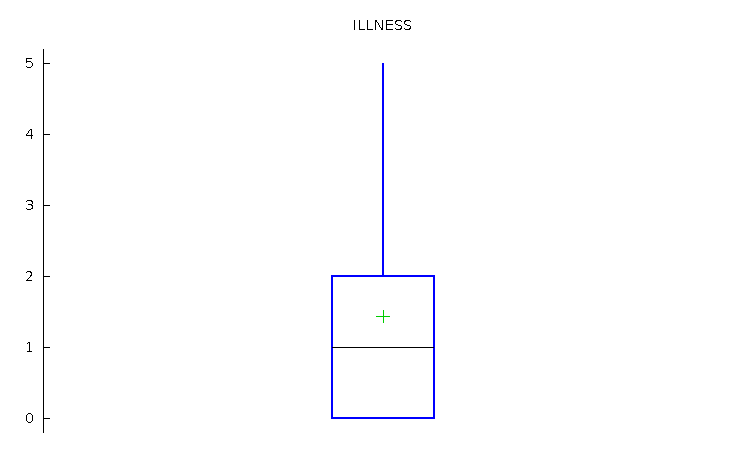
\includegraphics[width=0.475\textwidth]{figures/uboxplot} & 
    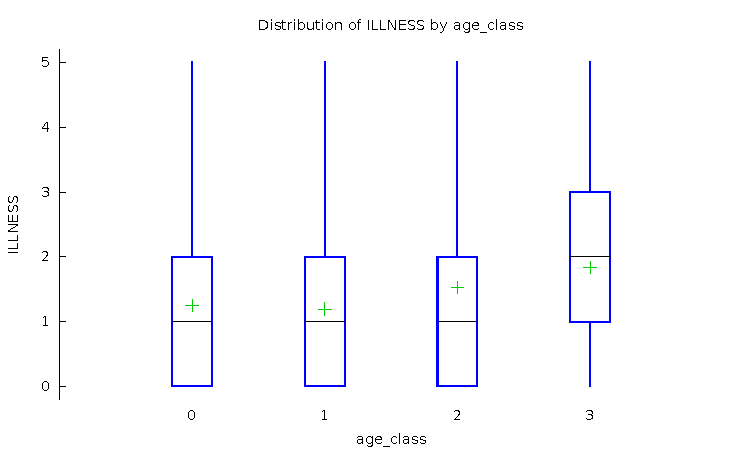
\includegraphics[width=0.475\textwidth]{figures/fboxplot}
  \end{tabular}
  \caption{Conditional and unconditional distribution of illnesses}
  \label{fig:fact-boxplots}
\end{figure}

%%% Local Variables: 
%%% mode: latex
%%% TeX-master: "gretl-guide"
%%% End: 


\chapter{Joining data sources}
\label{chap:join}

\section{Introduction}

Gretl provides two commands for adding data from file to an existing
dataset in the program's workspace, namely \texttt{append} and
\texttt{join}. The \texttt{append} command, which has been available
for a long time, is relatively simple and is described in the
\GCR. Here we focus on the \texttt{join} command, which is much more
flexible and sophisticated. This chapter gives an overview of the
functionality of \texttt{join} along with a detailed account of its
syntax and options. We provide several toy examples and discuss one
real-world case at length.

First, a note on terminology: in the following we use the terms 
``left-hand'' and ``inner'' to refer to the dataset that is already in
memory, and the terms ``right-hand'' and ``outer'' to refer to the
dataset in the file from which additional data are to be drawn. 

Two main features of \texttt{join} are worth emphasizing at the
outset:
\begin{itemize}
\item ``Key'' variables can be used to match specific observations
  (rows) in the inner and outer datasets, and this match need not be
  1 to 1.
\item A row filter may be applied to screen out unwanted observations
  in the outer dataset.
\end{itemize}

As will be explained below, these features support rather complex
concatenation and manipulation of data from different sources.

A further aspect of \texttt{join} should be noted---one that makes
this command particularly useful when dealing with very large data
files.  That is, when gretl executes a join operation it does not, in
general, read into memory the entire content of the right-hand side
dataset.  Only those columns that are actually needed for the
operation are read in full. This makes \texttt{join} faster and less
demanding of computer memory than the methods available in most other
software. On the other hand, gretl's asymmetrical treatment of the
``inner'' and ``outer'' datasets in \texttt{join} may require some
getting used to, for users of other packages.

\section{Basic syntax}
\label{sec:join-syntax}

The minimal invocation of \texttt{join} is

\qquad \texttt{join} \textsl{filename} \textsl{varname}

where \textsl{filename} is the name of a data file and
\textsl{varname} is the name of a series to be imported. Only two
sorts of data file are supported at present: delimited text files
(where the delimiter may be comma, space, tab or semicolon) and
``native'' gretl data files (\texttt{gdt} or \texttt{gdtb}).  A series
named \textsl{varname} may already be present in the left-hand
dataset, but that is not required. The series to be imported may be
numerical or string-valued. For most of the discussion below we assume
that just a single series is imported by each \texttt{join} command,
but see section~\ref{sec:join-multi} for an account of multiple
imports.

The effect of the minimal version of \texttt{join} is this: gretl
looks for a data column labeled \textsl{varname} in the specified
file; if such a column is found and the number of observations on the
right matches the number of observations in the current sample range
on the left, then the values from the right are copied into the
relevant range of observations on the left. If \textsl{varname} does
not already exist on the left, any observations outside of the current
sample are set to \texttt{NA}; if it exists already then observations
outside of the current sample are left unchanged.

The case where you want to rename a series on import is handled by the
\option{data} option. This option has one required argument, the name
by which the series is known on the right. At this point we need to
explain something about right-hand variable names (column
headings). 

\subsection{Right-hand names}
\label{subsec:rhnames}

We accept on input arbitrary column heading strings, but if these
strings do not qualify as valid gretl identifiers they are
automatically converted, and in the context of \texttt{join} you must
use the converted names. A gretl identifier must start with a letter,
contain nothing but (ASCII) letters, digits and the underscore
character, and must not exceed 31 characters. The rules used in name
conversion are:

\begin{enumerate}
\item Skip any leading non-letters.
\item Until the 31-character is reached or the input is exhausted:
  transcribe ``legal'' characters; skip ``illegal'' characters apart
  from spaces; and replace one or more consecutive spaces with an
  underscore, unless the last character transcribed is an underscore
  in which case space is skipped.
\end{enumerate}

In the unlikely event that this policy yields an empty string, we
replace the original with \texttt{col}\textsl{n}, where \textsl{n} is
replaced by the 1-based index of the column in question among those
used in the join operation. If you are in doubt regarding the
converted name of a given column, the function \texttt{fixname()} can
be used as a check: it takes the original string as an argument and
returns the converted name. Examples:

\begin{code}
? eval fixname("valid_identifier")
valid_identifier
? eval fixname("12. Some name")
Some_name
\end{code}

Returning to the use of the \option{data} option, suppose we have a
column headed \verb|"12. Some name"| on the right and wish to import
it as \texttt{x}. After figuring how the right-hand name converts, we
can do
%
\begin{code}
join foo.csv x --data="Some_name"
\end{code}

\section{Filtering}
\label{sec:join-filter}

Rows from the outer dataset can be filtered using the \verb|--filter|
option. The required parameter for this option is a Boolean condition,
that is, an expression which evaluates to non-zero (true, include the
row) or zero (false, skip the row) for each of the outer rows. The
filter expression may include any of the following terms: up to three
``right-hand'' series (under their converted names as explained
above); scalar or string variables defined ``on the left''; any of the
operators and functions available in gretl (including user-defined
functions); and numeric or string constants.

Here are a few simple examples of potentially valid filter options
(assuming that the specified right-hand side columns are found):

\begin{code}
# 1. relationship between two right-hand variables
--filter="x15<=x17"

# 2. comparison of right-hand variable with constant
--filter="nkids>2"

# 3. comparison of string-valued right-hand variable with string constant
--filter="SEX==\"F\""

# 4. filter on valid values of a right-hand variable
--filter=!missing(income)

# 5. compound condition
--filter="x < 100 && (x > 0 || y > 0)"
\end{code}

Note that if you are comparing against a string constant (as in
example 3 above) it is necessary to put the string in ``escaped''
double-quotes (each double-quote preceded by a backslash) so the
interpreter knows that \texttt{F} is not supposed to be the name of a
variable.

It is safest to enclose the whole filter expression in double quotes,
however this is not strictly required unless the expression contains
spaces or the equals sign.

In general, an error is flagged if a missing value is encountered in
a series referenced in a filter expression. This is because the
condition then becomes indeterminate; taking example 2 above, if the
\texttt{nkids} value is \texttt{NA} on any given row we are not in a
position to evaluate the condition \texttt{nkids>2}. However, you can
use the \texttt{missing()} function---or \texttt{ok()}, which is a
shorthand for \texttt{!missing()}---if you need a filter that keys off
the missing or non-missing status of a variable.


\section{Matching with keys}
\label{sec:join-keys}

Things get interesting when we come to key-matching. The purpose of
this facility is perhaps best introduced by example.  Suppose that (as
with many survey and census-based datasets) we have a dataset that is
composed of two or more related files, each having a different unit of
observation; for example we have a ``persons'' data file and a
``households'' data file. Table~\ref{tab:join-csv} shows a simple,
artificial case. The file \texttt{people.csv} contains a unique
identifier for the individuals, \texttt{pid}. The households file,
\texttt{hholds.csv}, contains the unique household identifier
\texttt{hid}, which is also present in the persons file.

As a first example of \texttt{join} with keys, let's add the
household-level variable \texttt{xh} to the persons dataset:
%
\begin{code}
open people.csv --quiet
join hholds.csv xh --ikey=hid
print --byobs
\end{code}

The basic key option is named \texttt{ikey}; this indicates ``inner
key'', that is, the key variable found in the left-hand or inner
dataset. By default it is assumed that the right-hand dataset contains
a column of the same name, though as we'll see below that assumption
can be overridden. The \texttt{join} command above says, find a series
named \texttt{xh} in the right-hand dataset and add it to the
left-hand one, using the values of \texttt{hid} to match rows.
Looking at the data in Table~\ref{tab:join-csv} we can see how this
should work. Persons 1 and 2 are both members of household 1, so they
should both get values of 1 for \texttt{xh}; persons 3 and 4 are
members of household 2, so that \texttt{xh} = 4; and so on. Note that
the order in which the key values occur on the right-hand side does
not matter.  The gretl output from the \texttt{print} command is shown
in the lower panel of Table~\ref{tab:join-csv}.

\begin{table}[thbp]
\begin{center}
\setlength{\tabcolsep}{4em}
\begin{tabular}{ll}
\texttt{people.csv} & \texttt{hholds.csv} \\[6pt]
\texttt{pid,hid,gender,age,xp} & \texttt{hid,country,xh} \\
\texttt{1,1,M,50,1} & \texttt{1,US,1} \\
\texttt{2,1,F,40,2} & \texttt{6,IT,12} \\
\texttt{3,2,M,30,3} & \texttt{3,UK,6} \\
\texttt{4,2,F,25,2} & \texttt{4,IT,8} \\
\texttt{5,3,M,40,3} & \texttt{2,US,4} \\
\texttt{6,4,F,35,4} & \texttt{5,IT,10} \\
\texttt{7,4,M,70,3} \\
\texttt{8,4,F,60,3} \\
\texttt{9,5,F,20,4} \\
\texttt{10,6,M,40,4}
\end{tabular}

\vspace{1em}

\begin{tabular}{rrr}
  \texttt{pid}  & \texttt{hid}   &  \texttt{xh} \\[6pt]
    \texttt{1}  &  \texttt{1}    &   \texttt{1} \\
    \texttt{2}  &  \texttt{1}    &   \texttt{1} \\
    \texttt{3}  &  \texttt{2}    &   \texttt{4} \\
    \texttt{4}  &  \texttt{2}    &   \texttt{4} \\
    \texttt{5}  &  \texttt{3}    &   \texttt{6} \\
    \texttt{6}  &  \texttt{4}    &   \texttt{8} \\
    \texttt{7}  &  \texttt{4}    &   \texttt{8} \\
    \texttt{8}  &  \texttt{4}    &   \texttt{8} \\
    \texttt{9}  &  \texttt{5}    &  \texttt{10} \\
   \texttt{10}  &  \texttt{6}    &  \texttt{12}
\end{tabular}
\caption{Two linked CSV data files, and the effect of a \texttt{join}}
\label{tab:join-csv}
\end{center}
\end{table}

Note that key variables are treated conceptually as integers. If a
specified key contains fractional values these are truncated.

Two extensions of the basic key mechanism are available.
\begin{itemize}
\item If the outer dataset contains a relevant key variable but it
  goes under a different name from the inner key, you can use the
  \verb|--okey| option to specify the outer key. (As with other
  right-hand names, this does not have to be a valid gretl
  identifier.) So, for example, if \texttt{hholds.csv} contained the
  \texttt{hid} information, but under the name \texttt{HHOLD}, the
  \texttt{join} command above could be modified as
  \begin{code}
  join hholds.csv xh --ikey=hid --okey=HHOLD
  \end{code}

\item If a single key is not sufficient to generate the matches you
  want, you can specify a double key in the form of two series names
  separated by a comma; in this case the importation of data is
  restricted to those rows on which both keys match. The syntax here
  is, for example
  \begin{code}
  join foo.csv x --ikey=key1,key2
  \end{code}
  Again, the \verb|--okey| option may be used if the corresponding
  right-hand columns are named differently. The same number of keys 
  must be given on the left and the right, but when a double key is
  used and only one of the key names differs on the right, the name
  that is in common may be omitted (although the comma separator must
  be retained). For example, the second of the following lines is
  acceptable shorthand for the first:
  \begin{code}
  join foo.csv x --ikey=key1,Lkey2 --okey=key1,Rkey2
  join foo.csv x --ikey=key1,Lkey2 --okey=,Rkey2
  \end{code}
\end{itemize}

\subsection{The number of key-matches}

The example shown in Table~\ref{tab:join-csv} is an instance of a 1 to
1 match: applying the matching criterion produces exactly one value of
the variable \texttt{xh} corresponding to each row of the inner
dataset. Two other possibilities arise: it may be that some rows in
the inner dataset have no match on the right, and/or some rows on the
left have multiple matches on the right. The latter case (``1 to $n$
matching'') is addressed in detail in the next section; here we
discuss the former.

The case where there's no match on the right is handled differently
depending on whether the join operation is adding a new series to the
inner dataset or modifying an existing one. If it's a new series, then
the unmatched rows automatically get \texttt{NA} for the imported
data. If, on the other hand, the join is pulling in values for a
series that is already present on the left, only matched rows will be
updated---or in other words, we do \textit{not} overwite an existing
value on the left with \texttt{NA} in the case where there's no match
on the right.

These defaults may not produce the desired results in every case but
gretl provides the means to modify the effect if need be.  We will
illustrate with two scenarios.

First, consider adding a new series recording ``number of hours
worked'' when the inner dataset contains individuals and the outer
file contains data on jobs. If an individual does not appear in the
jobs file, we may want to take her hours worked as implicitly zero
rather than \texttt{NA}. In this case gretl's \texttt{misszero()}
function can be used to turn \texttt{NA} into 0 in the imported
series.

Second, consider updating a series via join, when the outer file is
presumed to contain all available updated values, such that ``no
match'' should be taken as an implicit \texttt{NA}. In this case we
want the (presumably out-of-date) values on any unmatched rows to be
overwritten with \texttt{NA}. Let the series in question be called
\texttt{x} (both on the left and the right) and let the common key be
called \texttt{pid}. The solution is then
\begin{code}
join update.csv tmpvar --data=x --ikey=pid
x = tmpvar
\end{code}
As a new variable, \texttt{tmpvar} will get \texttt{NA} for all
unmatched rows; we then transcribe its values into \texttt{x}.  In a
more complicated case one might use the \texttt{smpl} command to limit
the sample range before assigning \texttt{tmpvar} to \texttt{x}, or
use the conditional assignment operator \texttt{?:}.

One further point should be mentioned here. Given some missing values
in an imported series you may sometimes want to know whether (a) 
the \texttt{NA}s were explicitly represented in the outer data file or
(b) they arose due to ``no match''. You can find this out by using
a method described in the following section, namely the \texttt{count}
variant of the aggregation option: this will give you a series with 0
values for all and only unmatched rows.

\section{Aggregation}
\label{sec:join-aggr}

In the case of 1 to $n$ matching of rows ($n > 1$) the user must
specify an ``aggregation method''; that is, a method for mapping from
$n$ rows down to one. This is handled by the \verb|--aggr| option
which requires a single argument from the following list:

\begin{center}
\begin{tabular}{ll}
\textit{Code} & \textit{Value returned} \\[6pt]
\texttt{count} & count of matches \\
\texttt{avg} & mean of matching values \\
\texttt{sum} & sum of matching values \\
\texttt{min} & minimum of matching values \\
\texttt{max} & maximum of matching values \\
\texttt{seq:}$i$ & the $i^{\rm th}$ matching 
  value (e.g.\ \texttt{seq:2}) \\
\texttt{min(}\textsl{aux}\texttt{)} & 
  minimum of matching values of auxiliary variable \\
\texttt{max(}\textsl{aux}\texttt{)} & 
  maximum of matching values of auxiliary variable\\
\end{tabular}
\end{center}

Note that the \texttt{count} aggregation method is special, in that
there is no need for a ``data series'' on the right; the imported
series is simply a function of the specified key(s). All the other
methods require that ``actual data'' are found on the right.  Also
note that when \texttt{count} is used, the value returned when no
match is found is (as one might expect) zero rather than \texttt{NA}.

The basic use of the \texttt{seq} method is shown above: following the
colon you give a positive integer representing the (1-based) position
of the observation in the sequence of matched rows. Alternatively, a
negative integer can be used to count down from the last match
(\texttt{seq:-1} selects the last match, \texttt{seq:-2} the
second-last match, and so on). If the specified sequence number is out
of bounds for a given observation this method returns \texttt{NA}.

Referring again to the data in Table~\ref{tab:join-csv}, suppose we
want to import data from the persons file into a dataset established
at household level.  Here's an example where we use the individual
\texttt{age} data from \texttt{people.csv} to add the average and
minimum age of household members.
\begin{code}
open hholds.csv --quiet
join people.csv avgage --ikey=hid --data=age --aggr=avg
join people.csv minage --ikey=hid --data=age --aggr=min
\end{code}

Here's a further example where we add to the household data the sum of
the personal data \texttt{xp}, with the twist that we apply filters to
get the sum specifically for household members under the age of 40,
and for women.
\begin{code}
open hholds.csv --quiet
join people.csv young_xp --ikey=hid --filter="age<40" --data=xp --aggr=sum
join people.csv female_xp --ikey=hid --filter="gender==\"F\"" --data=xp --aggr=sum
\end{code}

The possibility of using an auxiliary variable with the \texttt{min}
and \texttt{max} modes of aggregation gives extra flexibility. For
example, suppose we want for each household the income of its oldest
member:
\begin{code}
open hholds.csv --quiet
join people.csv oldest_xp --ikey=hid --data=xp --aggr=max(age)
\end{code}


\section{String-valued key variables}
\label{sec:join-strings}

The examples above use numerical variables (household and individual
ID numbers) in the matching process. It is also possible to use
string-valued variables, in which case a match means that the string
values of the key variables compare equal (with case sensitivity). 
When using double keys, you can mix numerical and string keys, but
naturally you cannot mix a string variable on the left (via
\texttt{ikey}) with a numerical one on the right (via \texttt{okey}),
or vice versa.

Here's a simple example. Suppose that alongside \texttt{hholds.csv} we
have a file \texttt{countries.csv} with the following content:
\begin{code}
 country,GDP
 UK,100
 US,500
 IT,150
 FR,180
\end{code}

The variable \texttt{country}, which is also found in
\texttt{hholds.csv}, is string-valued. We can pull the GDP of the
country in which the household resides into our households dataset
with
\begin{code}
open hholds.csv -q
join countries.csv GDP --ikey=country
\end{code}
which gives
\begin{code}
           hid      country          GDP

1            1            1          500
2            6            2          150
3            3            3          100
4            4            2          150
5            2            1          500
6            5            2          150
\end{code}

\section{Importing multiple series}
\label{sec:join-multi}

The examples given so far have been limited in one respect. While
several columns in the outer data file may be referenced (as keys, or
in filtering or aggregation) only one column has actually provided
data---and correspondingly only one series in the inner dataset has
been created or modified---per invocation of \texttt{join}. However,
\texttt{join} can handle the importation of several series at
once. This section gives an account of the required syntax along with
certain restrictions that apply to the multiple-import case.

There are two ways to specify more than one series for importation:
\begin{enumerate}
\item The \textsl{varname} field in the command can take the form of
  a space-separated list of names rather than a single name.
\item Alternatively, you can give the name of an array of strings
  in place of \textsl{varname}: the elements of this array should be
  the names of the series to import.
\end{enumerate}

Here are the limitations:
\begin{enumerate}
\item The \verb|--data| option, which permits the renaming of a series
  on import, is not available. When importing multiple series you
  are obliged to accept their ``outer'' names, fixed up as described
  in section~\ref{subsec:rhnames}.
\item While the other \texttt{join} options are available, they
  necessarily apply uniformly to all the series imported via a given
  command. This means that if you want to import several series but
  using different keys, filters or aggregation methods you must use a
  sequence of commands.
\end{enumerate}

Here are a couple of examples of multiple imports.
\begin{code}
# open base datafile containing keys
open PUMSdata.gdt

# join using a list of import names
join ss13pnc.csv SCHL WAGP WKHP --ikey=SERIALNO,SPORDER

# using a strings array: may be worthwhile if the array
# will be used for more than one purpose
strings S = array(3)
S[1] = "SCHL"
S[2] = "WAGP"
S[3] = "WKHP"
join ss13pnc.csv S --ikey=SERIALNO,SPORDER
\end{code}

\section{A real-world case}
\label{sec:join-SHIW}

For a real use-case for \texttt{join} with cross-sectional data, we
turn to the Bank of Italy's \textit{Survey on Household Income and
  Wealth} (SHIW).\footnote{Details of the survey can be found at
  \url{http://www.bancaditalia.it/statistiche/indcamp/bilfait/dismicro}.
  The ASCII (CSV) data files for the 2010 survey are available at
  \url{http://www.bancaditalia.it/statistiche/indcamp/bilfait/dismicro/annuale/ascii/ind10_ascii.zip}.}
In ASCII form the 2010 survey results comprise 47\,MB of data in 29
files. In this exercise we will draw on five of the SHIW files to
construct a replica of the dataset used in Thomas Mroz's famous paper
\citep{mroz87} on women's labor force participation, which contains
data on married women between the age of 30 and 60 along with certain
characteristics of their households and husbands.

Our general strategy is as follows: we create a ``core'' dataset by
opening the file \texttt{carcom10.csv}, which contains basic data on
the individuals. After dropping unwanted individuals (all but married
women), we use the resulting dataset as a base for pulling in further
data via the \texttt{join} command.

The complete script to do the job is given in the Appendix to this
chapter; here we walk through the script with comments interspersed.
We assume that all the relevant files from the Bank of Italy survey
are contained in a subdirectory called \texttt{SHIW}.

Starting with \texttt{carcom10.csv}, we use the \verb|--cols| option
to the \texttt{open} command to import specific series, namely
\texttt{NQUEST} (household ID number), \texttt{NORD} (sequence number
for individuals within each household), \texttt{SEX} (male = 1, female
= 2), \texttt{PARENT} (status in household: 1 = head of household, 2 =
spouse of head, etc.), \texttt{STACIV} (marital status: married = 1),
\texttt{STUDIO} (educational level, coded from 1 to 8),
\texttt{ETA} (age in years) and \texttt{ACOM4C} (size of town).
%
\begin{code}
open SHIW/carcom10.csv --cols=1,2,3,4,9,10,29,41
\end{code}
%
We then restrict the sample to married women from 30 to 60 years of
age, and additionally restrict the sample of women to those who are
either heads of households or spouses of the head.
%
\begin{code}
smpl SEX==2 && ETA>=30 && ETA<=60 && STACIV==1 --restrict
smpl PARENT<3  --restrict
\end{code}
%
For compatibility with the Mroz dataset as presented in the gretl
data file \texttt{mroz87.gdt}, we rename the age and education
variables as \texttt{WA} and \texttt{WE} respectively, we compute the
\texttt{CIT} dummy and finally we
store the reduced base dataset in gretl format.
%
\begin{code}
rename ETA WA
rename STUDIO WE
series CIT = (ACOM4C > 2)

store mroz_rep.gdt
\end{code}

The next step will be to get data on working hours from the jobs file
\texttt{allb1.csv}. There's a complication here. We need the total
hours worked over the course of the year (for both the women and their
husbands). This is not available as such, but the variables
\texttt{ORETOT} and \texttt{MESILAV} give, respectively, average hours
worked per week and the number of months worked in 2010, each on a
per-job basis. If each person held at most one job over the year we
could compute his or her annual hours as
\begin{code}
HRS = ORETOT * 52 * MESILAV/12
\end{code}
However, some people had more than one job, and in this case what we
want is the sum of annual hours across their jobs.  We could use
\texttt{join} with the \texttt{seq} aggregation method to construct
this sum, but it is probably more straightforward to read the
\texttt{allb1} data, compute the \texttt{HRS} values per job as shown
above, and save the results to a temporary CSV file.
%
\begin{code}
open SHIW/allb1.csv --cols=1,2,8,11 --quiet
series HRS = misszero(ORETOT) * 52 * misszero(MESILAV)/12
store HRS.csv NQUEST NORD HRS
\end{code}

Now we can reopen the base dataset and join the hours variable from
\texttt{HRS.csv}.  Note that we need a double key here: the women are
uniquely identified by the combination of \texttt{NQUEST} and
\texttt{NORD}. We don't need an \texttt{okey} specification since
these keys go under the same names in the right-hand file. We define
labor force participation, \texttt{LFP}, based on hours.
%
\begin{code}
open mroz_rep.gdt
join HRS.csv WHRS --ikey=NQUEST,NORD --data=HRS --aggr=sum
WHRS = misszero(WHRS)
LFP = WHRS > 0
\end{code}
%
For reference, here's how we could have used \texttt{seq} to avoid
writing a temporary file:
%
\begin{code}
join SHIW/allb1.csv njobs --ikey=NQUEST,NORD --data=ORETOT --aggr=count
series WHRS = 0
loop i=1..max(njobs) -q
  join SHIW/allb1.csv htmp --ikey=NQUEST,NORD --data=ORETOT --aggr="seq:$i"
  join SHIW/allb1.csv mtmp --ikey=NQUEST,NORD --data=MESILAV --aggr="seq:$i"
  WHRS += misszero(htmp) * 52 * misszero(mtmp)/12 
endloop
\end{code}

To generate the work experience variable, \texttt{AX}, we use the file
\texttt{lavoro.csv}: this contains a variable named \texttt{ETALAV}
which records the age at which the person first started work.
%
\begin{code}
join SHIW/lavoro.csv ETALAV --ikey=NQUEST,NORD
series AX = misszero(WA - ETALAV)
\end{code}
%
We compute the woman's hourly wage, \texttt{WW}, as the ratio of total
employment income to annual working hours.  This requires drawing the
series \texttt{YL} (payroll income) and \texttt{YM} (net
self-employment income) from the persons file \texttt{rper10.csv}.
%
\begin{code}
join SHIW/rper10.csv YL YM --ikey=NQUEST,NORD --aggr=sum
series WW = LFP ? (YL + YM)/WHRS : 0
\end{code}
%
The family's net disposable income is available as \texttt{Y} in the file
\texttt{rfam10.csv}; we import this as \texttt{FAMINC}.
%
\begin{code}
join SHIW/rfam10.csv FAMINC --ikey=NQUEST --data=Y
\end{code}
%
Data on number of children are now obtained by applying the
\texttt{count} method. For the Mroz replication we want the number of
children under the age of 6, and also the number aged 6 to 18.
%
\begin{code}
join SHIW/carcom10.csv KIDS --ikey=NQUEST --aggr=count --filter="ETA<=18"
join SHIW/carcom10.csv KL6 --ikey=NQUEST --aggr=count --filter=ETA<6
series K618 = KIDS - KL6
\end{code}
%
We want to add data on the women's husbands, but how do we find them?
To do this we create an additional inner key which we'll call
\verb|H_ID| (husband ID), by sub-sampling in turn on the observations
falling into each of two classes: (a) those where the woman is
recorded as head of household and (b) those where the husband has that
status. In each case we want the individual ID (\texttt{NORD}) of the
household member whose status is complementary to that of the woman in
question. So for case (a) we subsample using \texttt{PARENT==1} (head
of household) and filter the join using \texttt{PARENT==2} (spouse of
head); in case (b) we do the converse. We thus construct \verb|H_ID|
piece-wise.
%
\begin{code}
# for women who are household heads
smpl PARENT==1 --restrict --replace
join SHIW/carcom10.csv H_ID --ikey=NQUEST --data=NORD --filter="PARENT==2"
# for women who are not household heads
smpl PARENT==2 --restrict --replace
join SHIW/carcom10.csv H_ID --ikey=NQUEST --data=NORD --filter="PARENT==1"
smpl full
\end{code}
%
Now we can use our new inner key to retrieve the husbands' data,
matching \verb|H_ID| on the left with \texttt{NORD} on the right
within each household.
%
\begin{code}
join SHIW/carcom10.csv HA --ikey=NQUEST,H_ID --okey=NQUEST,NORD --data=ETA
join SHIW/carcom10.csv HE --ikey=NQUEST,H_ID --okey=NQUEST,NORD --data=STUDIO
join HRS.csv HHRS --ikey=NQUEST,H_ID --okey=NQUEST,NORD --data=HRS --aggr=sum
HHRS = misszero(HHRS)
\end{code}
%
The remainder of the script is straightforward and does not require
discussion here: we recode the education variables for compatibility;
delete some intermediate series that are not needed any more; add
informative labels; and save the final product. See the Appendix for
details.

To compare the results from this dataset with those from the earlier
US data used by Mroz, one can copy the input file \texttt{heckit.inp}
(supplied with the gretl package) and substitute \verb|mroz_rep.gdt|
for \texttt{mroz87.gdt}. It turns out that the results are
qualitatively very similar.

\section{The representation of dates}
\label{sec:join-isodates}

Up to this point all the data we have considered have been
cross-sectional. In the following sections we discuss data that have a
time dimension, and before proceeding it may be useful to say
something about the representation of dates. Gretl takes the ISO 8601
standard as its reference point but provides mean of converting dates
provided in other formats; it also offers a set of calendrical
functions for manipulating dates (\texttt{isodate}, \texttt{isoconv},
\texttt{epochday} and others).

ISO 8601 recognizes two formats for daily dates, ``extended'' and
``basic''. In both formats dates are given as 4-digit year, 2-digit
month and 2-digit day, in that order. In extended format a dash is
inserted between the fields---as in \texttt{2013-10-21} or more
generally \texttt{YYYY-MM-DD}---while in basic format the fields are
run together (\texttt{YYYYMMDD}). Extended format is more easily
parsed by human readers while basic format is more suitable for
computer processing, since one can apply ordinary arithmetic to
compare dates as equal, earlier or later.  The standard also
recognizes \texttt{YYYY-MM} as representing year and month, e.g.\
\texttt{2010-11} for November 2010,\footnote{The form \texttt{YYYYMM}
  is \textit{not} recognized for year and month.} as well as
a plain four-digit number for year alone.

One problem for economists is that the ``quarter'' is not a period
covered by ISO 8601. This could be presented by \texttt{YYYY-Q} (with
only one digit following the dash) but in gretl output we in fact use
a colon, as in \texttt{2013:2} for the second quarter of 2013. (For
printed output of months gretl also uses a colon, as in
\texttt{2013:06}. A difficulty with following ISO here is that in a
statistical context a string such as \texttt{1980-10} may look more
like a subtraction than a date.)  Anyway, at present we are more
interested in the parsing of dates on input rather than in what gretl
prints. And in that context note that ``excess precision'' is
acceptable: a month may be represented by its first day (e.g.\
\texttt{2005-05-01} for May, 2005), and a quarter may be represented
by its first month and day (\texttt{2005-07-01} for the third quarter
of 2005).

Some additional points regarding dates will be taken up as they become
relevant in practical cases of joining data.

\section{Time-series data}
\label{sec:join-timeser}

Suppose our left-hand dataset is recognized by gretl as time series
with a supported frequency (annual, quarterly, monthly, weekly, daily
or hourly). This will be the case if the original data were read from
a file that contained suitable time or date information, or if a
time-series interpretation has been imposed using either the
\texttt{setobs} command or its GUI equivalent.  Then---apart, perhaps,
from some very special cases---joining additional data is bound to
involve matching observations by time-period. 

In this case, contrary to the cross-sectional case, the inner dataset
has a natural ordering which gretl is aware of; hence, no ``inner
key'' is required. All we need is a means of identifying the period on
the right and this is why, in a time-series context, we'll refer to
the outer key as the ``time key''. Most likely, this information will
appear in a single column in the outer data file, often but not always
the first column.

The \texttt{join} command provides a simple (but limited) default for
extracting period information from the outer data file, plus an
option that can be used if the default is not applicable, as follows.
\begin{itemize}
\item The default assumptions are: (1) the time key appears in the
  first column; (2) the heading of this column is either left blank or
  is one of \texttt{obs}, \texttt{date}, \texttt{year},
  \texttt{period}, \texttt{observation}, or \verb|observation_date|
  (on a case-insensitive comparison); and (3) the time format conforms
  to ISO 8601 where applicable (``extended'' daily date format
  \texttt{YYYY-MM-DD}, monthly format \texttt{YYYY-MM}, or annual
  format \texttt{YYYY}).
\item If dates do not appear in the first column of the outer file, or
  if the column heading or format is not as just described, the
  \option{tkey} option can be used to indicate which column should be
  used and/or what format should be assumed.
\end{itemize}

\subsection{Setting the time-key column and/or format}

The \option{tkey} option requires a parameter holding the name of the
column in which the time key is located and/or a string specifying the
format in which dates/times are written in the time-key column. This
parameter should be enclosed in double-quotes. If both elements are
present they should be separated by a comma; if only a format is given
it should be preceded by a comma. Some examples:

\begin{code}
--tkey="Period,%m/%d/%Y"
--tkey="Period"
--tkey="obsperiod"
--tkey=",%Ym%m"
\end{code}

The first of these applies if \texttt{Period} is not the first column
on the right, and dates are given in the US format of month, day,
year, separated by slashes. The second implies that although
\texttt{Period} is not the first column, the date format is ISO 8601.
The third again implies that the date format is OK; here the name is
required even if \texttt{obsperiod} is the first column since this
heading is not one recognized by gretl's heuristic. The last example
implies that dates are in the first column (with one of the recognized
headings), but are given in the non-standard format year,
``\texttt{m}'', month.

The date format string should be composed using the codes employed by
the POSIX function \texttt{strptime}; Table \ref{tab:join-datefmt}
contains a list of the most relevant codes.\footnote{The
  \texttt{\%q} code for quarter is not present in \texttt{strptime};
  it is added for use with \texttt{join} since quarterly data are
  common in macroeconomics.}

\begin{table}[htbp]
  \centering
  \begin{tabular}{rp{0.7\textwidth}}
    \textbf{Code} & \textbf{Meaning} \\
    \hline
    \verb|%%| & The \% character. \\
    \verb|%b| & The month name according to the current locale,
    either abbreviated or in full.\\
    \verb|%C| & The century number (0--99).\\
    \verb|%d| & The day of month (1--31). \\
    \verb|%D| & Equivalent to \verb|%m/%d/%y|.  (This is the American
    style date, very  confusing  to  non-Americans, especially
    since \verb|%d/%m/%y| is widely used in Europe.  The 
    ISO 8601 standard format is \verb|%Y-%m-%d|.) \\
    \verb|%H| & The hour (0--23).\\
    \verb|%j| & The day number in the year (1--366).\\
    \verb|%m| & The month number (1--12).\\
    \verb|%n| & Arbitrary whitespace.\\
    \verb|%q| & The quarter (1--4).\\
    \verb|%w| & The weekday number (0--6) with Sunday = 0.\\
    \verb|%y| & The year within century (0--99).  When a century is
    not otherwise specified, values in  the  range  69--99  refer
    to  years  in  the  twentieth  century (1969--1999);  values
    in the range 00--68 refer to years in the twenty-first century (2000--2068).\\
    \verb|%Y| &  The year, including century (for example, 1991).\\
    \hline
  \end{tabular}
  \caption{Date format codes}
  \label{tab:join-datefmt}
\end{table}

\subsection{Example: daily stock prices}

We show below the first few lines of a file named \texttt{IBM.csv}
containing stock-price data for IBM corporation.

\begin{code}
Date,Open,High,Low,Close,Volume,Adj Close
2013-08-02,195.50,195.50,193.22,195.16,3861000,195.16
2013-08-01,196.65,197.17,195.41,195.81,2856900,195.81
2013-07-31,194.49,196.91,194.49,195.04,3810000,195.04
\end{code}

Note that the data are in reverse time-series order---that won't
matter to \texttt{join}, the data can appear in any order. Also note
that the first column is headed \texttt{Date} and holds daily dates as
ISO 8601 extended. That means we can pull the data into gretl very
easily. In the following fragment we create a suitably dimensioned
empty daily dataset then rely on the default behavior of \texttt{join}
with time-series data to import the closing stock price.

\begin{code}
nulldata 500
setobs 5 2012-01-01
join IBM.csv Close
\end{code}

To make explicit what we're doing, we could accomplish exactly the
same using the \option{tkey} option:

\begin{code}
join IBM.csv Close --tkey="Date,%Y-%m-%d"
\end{code}

\subsection{Example: OECD quarterly data}

Table~\ref{tab:oecd-gdp} shows an excerpt from a CSV file provided
by the OECD statistical site (\url{stat.oecd.org}) in response to a
request for GDP at constant prices for several
countries.\footnote{Retrieved 2013-08-05. The OECD files in fact
  contain two leading columns with very long labels; these are irrelevant
  to the present example and can be omitted without altering the
  sample script.}

\begin{table}[htbp]
\begin{code}
Frequency,Period,Country,Value,Flags
"Quarterly","Q1-1960","France",463876.148126845,E
"Quarterly","Q1-1960","Germany",768802.119278467,E
"Quarterly","Q1-1960","Italy",414629.791450547,E
"Quarterly","Q1-1960","United Kingdom",578437.090291889,E
"Quarterly","Q2-1960","France",465618.977328614,E
"Quarterly","Q2-1960","Germany",782484.138122549,E
"Quarterly","Q2-1960","Italy",420714.910290157,E
"Quarterly","Q2-1960","United Kingdom",572853.474696578,E
"Quarterly","Q3-1960","France",469104.41925852,E
"Quarterly","Q3-1960","Germany",809532.161494483,E
"Quarterly","Q3-1960","Italy",426893.675840156,E
"Quarterly","Q3-1960","United Kingdom",581252.066618986,E
"Quarterly","Q4-1960","France",474664.327992619,E
"Quarterly","Q4-1960","Germany",817806.132384948,E
"Quarterly","Q4-1960","Italy",427221.338414114,E
...
\end{code}
\caption{Example of CSV file as provided by the OECD statistical
  website}
\label{tab:oecd-gdp}  
\end{table}

This is an instance of data in what we call \emph{atomic format}, that
is, a format in which each line of the outer file contains a single
data-point and extracting data mainly requires filtering the appropriate
lines. The outer time key is under the \texttt{Period} heading, and
has the format \texttt{Q\emph{<quarter>-<year>}}. Assuming that the
file in Table~\ref{tab:oecd-gdp} has the name \texttt{oecd.csv}, the
following script reconstructs the time series of Gross Domestic
Product for several countries:

\begin{footnotesize}
\begin{verbatim}
nulldata 220
setobs 4 1960:1

join oecd.csv FRA --tkey="Period,Q%q-%Y" --data=Value --filter="Country==\"France\""
join oecd.csv GER --tkey="Period,Q%q-%Y" --data=Value --filter="Country==\"Germany\""
join oecd.csv ITA --tkey="Period,Q%q-%Y" --data=Value --filter="Country==\"Italy\""
join oecd.csv  UK --tkey="Period,Q%q-%Y" --data=Value --filter="Country==\"United Kingdom\""
\end{verbatim}
\end{footnotesize}

Note the use of the format codes \verb|%q| for the quarter and
\verb|%Y| for the 4-digit year. A touch of elegance could
have been added by storing the invariant options to \cmd{join} using
the \cmd{setopt} command, as in

\begin{footnotesize}
\begin{verbatim}
setopt join persist --tkey="Period,Q%q-%Y" --data=Value
join oecd.csv FRA --filter="Country==\"France\""
join oecd.csv GER --filter="Country==\"Germany\""
join oecd.csv ITA --filter="Country==\"Italy\""
join oecd.csv  UK --filter="Country==\"United Kingdom\""
setopt join clear
\end{verbatim}
\end{footnotesize}

If one were importing a large number of such series it might be worth
rewriting the sequence of joins as a loop, as in

\begin{footnotesize}
\begin{verbatim}
sprintf countries "France Germany Italy \"United Kingdom\""
sprintf vnames "FRA GER ITA UK"
setopt join persist --tkey="Period,Q%q-%Y" --data=Value

loop foreach i @countries
  string vname = strsplit(vnames, i)
  join oecd.csv @vname --filter="Country==\"$i\""
endloop
setopt join clear
\end{verbatim}
\end{footnotesize}

\section{Special handling of time columns}
\label{sec:join-tconvert}

When dealing with straight time series data the \texttt{tkey}
mechanism described above should suffice in almost all cases. In some
contexts, however, time enters the picture in a more complex way;
examples include panel data (see section~\ref{sec:join-panel}) and
so-called realtime data (see chapter~\ref{chap:realtime}). To handle
such cases \texttt{join} provides the \option{tconvert} option. This
can be used to select certain columns in the right-hand data file for
special treatment: strings representing dates in these columns will be
converted to numerical values: 8-digit numbers on the pattern
\texttt{YYYYMMDD} (ISO basic daily format).  Once dates are in this
form it is easy to use them in key-matching or filtering.

By default it is assumed that the strings in the selected columns are
in ISO extended format, \texttt{YYYY-MM-DD}. If that is not
the case you can supply a time-format string using the
\option{tconv-fmt} option. The format string should be written using
the codes shown in Table~\ref{tab:join-datefmt}.

Here are some examples:

\begin{code}
# select one column for treatment
--tconvert=start_date

# select two columns for treatment
--tconvert="start_date,end_date"

# specify US-style daily date format
--tconv-fmt="%m/%d/%Y"

# specify quarterly date-strings (as in 2004q1)
--tconv-fmt="%Yq%q"
\end{code}

Some points to note:

\begin{itemize}
\item If a specified column is not selected for a substantive role in
  the join operation (as data to be imported, as a key, or as an
  auxiliary variable for use in aggregation) the column in question is
  not read and so no conversion is carried out.
\item If a specified column contains numerical rather than string
  values, no conversion is carried out.
\item If a string value in a selected column fails parsing using the
  relevant time format (user-specified or default), the converted
  value is \texttt{NA}.
\item On successful conversion, the output is always in daily-date
  form as stated above. If you specify a monthly or quarterly time
  format, the converted date is the first day of the month or quarter.
\end{itemize}


\section{Panel data}
\label{sec:join-panel}

In section~\ref{sec:join-timeser} we gave an example of reading
quarterly GDP data for several countries from an OECD file. In that
context we imported each country's data as a distinct time-series
variable. Now suppose we want the GDP data in panel format instead
(stacked time series). How can we do this with \texttt{join}? 

As a reminder, here's what the OECD data look like:
\begin{code}
Frequency,Period,Country,Value,Flags
"Quarterly","Q1-1960","France",463876.148126845,E
"Quarterly","Q1-1960","Germany",768802.119278467,E
"Quarterly","Q1-1960","Italy",414629.791450547,E
"Quarterly","Q1-1960","United Kingdom",578437.090291889,E
"Quarterly","Q2-1960","France",465618.977328614,E
\end{code}
and so on. If we have four countries and quarterly observations
running from 1960:1 to 2013:2 ($T$ = 214 quarters) we might set up our
panel workspace like this:
\begin{code}
scalar N = 4
scalar T = 214
scalar NT = N*T
nulldata NT --preserve
setobs T 1.1 --stacked-time-series
\end{code}

The relevant outer keys are obvious: \texttt{Country} for the country
and \texttt{Period} for the time period. Our task is now to construct
matching keys in the inner dataset. This can be done via two
panel-specific options to the \texttt{setobs} command. Let's work on
the time dimension first:
\begin{code}
setobs 4 1960:1 --panel-time
series quarter = $obsdate
\end{code}
This variant of \texttt{setobs} allows us to tell gretl that time in
our panel is quarterly, starting in the first quarter of 1960. Having
set that, the accessor \verb|$obsdate| will give us a series of
8-digit dates representing the first day of each quarter---19600101,
19600401, 19600701, and so on, repeating for each country. As we
explained in section~\ref{sec:join-tconvert}, we can use the
\option{tconvert} option on the outer series \texttt{Period} to get
exactly matching values (in this case using a format of \verb|Q%q-%Y|
for parsing the \texttt{Period} values).

Now for the country names:
\begin{code}
string cstrs
sprintf cstrs "France Germany Italy \"United Kingdom\""
setobs country cstrs --panel-groups
\end{code}
Here we write into the string \texttt{cstrs} the names of the
countries, using escaped double-quotes to handle the space in ``United
Kingdom'', then pass this string to \texttt{setobs} with the
\option{panel-groups} option, preceded by the identifier
\texttt{country}. This asks gretl to construct a string-valued series
named \texttt{country}, in which each name will repeat $T$ times.

We're now ready to join. Assuming the OECD file is named
\texttt{oecd.csv} we do
\begin{code}
join oecd.csv GDP --data=Value \
 --ikey=country,quarter --okey=Country,Period \
 --tconvert=Period --tconv-fmt="Q%q-%Y"
\end{code}

\subsection{Other input formats}

The OECD file discussed above is in the most convenient format for
\texttt{join}, with one data-point per line. But sometimes we may want
to make a panel from a data file structured like this:
\begin{code}
# Real GDP
Period,France,Germany,Italy,"United Kingdom"
"Q1-1960",463863,768757,414630,578437
"Q2-1960",465605,782438,420715,572853
"Q3-1960",469091,809484,426894,581252
"Q4-1960",474651,817758,427221,584779
"Q1-1961",482285,826031,442528,594684
...
\end{code}

Call this file \verb|side_by_side.csv|.  Assuming the same initial
set-up as above, we can panelize the data by setting the sample to
each country's time series in turn and importing the relevant
column. The only point to watch here is that the string ``United
Kingdom'', being a column heading, will become \verb|United_Kingdom|
on importing (see section~\ref{sec:join-syntax}) so we'll need a
slightly different set of country strings.
%
\begin{code}
sprintf cstrs "France Germany Italy United_Kingdom"
setobs country cstrs --panel-groups
loop foreach i @cstrs --quiet
  smpl country=="$i" --restrict --replace
  join side_by_side.csv GDP --data=$i \
  --ikey=quarter --okey=Period \
  --tconvert=Period --tconv-fmt="Q%q-%Y"
endloop
smpl full
\end{code}

If our working dataset and the outer data file are dimensioned such
that there are just as many time-series observations on the right as
there are time slots on the left---and the observations on the right
are contiguous, in chronological order, and start on the same date as
the working dataset---we could dispense with the key apparatus and
just use the first line of the \texttt{join} command shown
above. However, in general it is safer to use keys to ensure that the
data end up in correct registration.

\section{Memo: \texttt{join} options}
\label{sec:join-options}

Basic syntax: \texttt{join} \textsl{filename} \textsl{varname(s)} [
\textsl{options} ]

\begin{center}
\begin{tabular}{lp{.7\textwidth}}
  \textit{flag} & \textit{effect} \\ [6pt]
  \verb|--data| & Give the name of the data column on the right, in
                  case it differs from \textsl{varname}
                  (\ref{sec:join-syntax}); single import only  \\
  \verb|--filter| & Specify a condition for filtering data rows
                    (\ref{sec:join-filter}) \\
  \verb|--ikey| & Specify up to two keys for matching data rows
                  (\ref{sec:join-keys}) \\
  \verb|--okey| & Specify outer key name(s) in case they
                  differ the inner ones (\ref{sec:join-keys})\\
  \verb|--aggr| & Select an aggregation method for 1 to $n$ joins
                 (\ref{sec:join-aggr}) \\ 
  \verb|--tkey| & Specify right-hand time key (\ref{sec:join-timeser}) \\
  \verb|--tconvert| & Select outer date columns for conversion to
                      numeric form (\ref{sec:join-tconvert}) \\
  \verb|--tconv-fmt| & Specify a format for use with \texttt{tconvert} 
                       (\ref{sec:join-tconvert}) \\
  \verb|--verbose| & Report on progress in reading the outer data
\end{tabular}
\end{center}


\pagebreak[4]

\section*{Appendix: the full Mroz data script}

\begin{code}
# start with everybody; get gender, age and a few other variables 
# directly while we're at it
open SHIW/carcom10.csv --cols=1,2,3,4,9,10,29,41

# subsample on married women between the ages of 30 and 60
smpl SEX==2 && ETA>=30 && ETA<=60 && STACIV==1 --restrict
# for simplicity, restrict to heads of households and their spouses
smpl PARENT<3  --restrict

# rename the age and education variables for compatibility; compute
# the "city" dummy and finally save the reduced base dataset
rename ETA WA
rename STUDIO WE
series CIT = (ACOM4C>2)
store mroz_rep.gdt

# make a temp file holding annual hours worked per job
open SHIW/allb1.csv --cols=1,2,8,11 --quiet
series HRS = misszero(ORETOT) * 52 * misszero(MESILAV)/12
store HRS.csv NQUEST NORD HRS

# reopen the base dataset and begin drawing assorted data in
open mroz_rep.gdt

# women's annual hours (summed across jobs) 
join HRS.csv WHRS --ikey=NQUEST,NORD --data=HRS --aggr=sum
WHRS = misszero(WHRS)

# labor force participation
LFP = WHRS > 0

# work experience: ETALAV = age when started first job
join SHIW/lavoro.csv ETALAV --ikey=NQUEST,NORD
series AX = misszero(WA - ETALAV)

# women's hourly wages
join SHIW/rper10.csv YL YM --ikey=NQUEST,NORD --aggr=sum
series WW = LFP ? (YL + YM)/WHRS : 0

# family income (Y = net disposable income)
join SHIW/rfam10.csv FAMINC --ikey=NQUEST --data=Y

# get data on children using the "count" method
join SHIW/carcom10.csv KIDS --ikey=NQUEST --aggr=count --filter="ETA<=18"
join SHIW/carcom10.csv KL6 --ikey=NQUEST --aggr=count --filter=ETA<6
series K618 = KIDS - KL6

# data on husbands: we first construct an auxiliary inner key for 
# husbands, using the little trick of subsampling the inner dataset
#
# for women who are household heads
smpl PARENT==1 --restrict --replace
join SHIW/carcom10.csv H_ID --ikey=NQUEST --data=NORD --filter="PARENT==2"
# for women who are not household heads
smpl PARENT==2 --restrict --replace
join SHIW/carcom10.csv H_ID --ikey=NQUEST --data=NORD --filter="PARENT==1"
smpl full

# add husbands' data via the newly-added secondary inner key
join SHIW/carcom10.csv HA --ikey=NQUEST,H_ID --okey=NQUEST,NORD --data=ETA
join SHIW/carcom10.csv HE --ikey=NQUEST,H_ID --okey=NQUEST,NORD --data=STUDIO
join HRS.csv HHRS --ikey=NQUEST,H_ID --okey=NQUEST,NORD --data=HRS --aggr=sum
HHRS = misszero(HHRS)

# final cleanup begins

# recode educational attainment as years of education
matrix eduyrs = {0, 5, 8, 11, 13, 16, 18, 21}
series WE = replace(WE, seq(1,8), eduyrs)
series HE = replace(HE, seq(1,8), eduyrs)

# cut some cruft
delete SEX STACIV KIDS YL YM PARENT H_ID ETALAV

# add some labels for the series
setinfo LFP -d "1 if woman worked in 2010"
setinfo WHRS -d "Wife's hours of work in 2010"
setinfo KL6 -d "Number of children less than 6 years old in household"
setinfo K618 -d "Number of children between ages 6 and 18 in household"
setinfo WA -d "Wife's age"
setinfo WE -d "Wife's educational attainment, in years"
setinfo WW -d "Wife's average hourly earnings, in 2010 euros"
setinfo HHRS -d "Husband's hours worked in 2010"
setinfo HA -d "Husband's age"
setinfo HE -d "Husband's educational attainment, in years"
setinfo FAMINC -d "Family income, in 2010 euros"
setinfo AX -d "Actual years of wife's previous labor market experience"
setinfo CIT -d "1 if live in large city"

# save the final product
store mroz_rep.gdt
\end{code}

    
%%% Local Variables: 
%%% mode: latex
%%% TeX-master: "gretl-guide"
%%% End: 

\chapter{Realtime data}
\label{chap:realtime}

\section{Introduction}
\label{sec:realtime-intro}

As of \app{gretl} version 1.9.13 the \cmd{join} command (see chapter
\ref{chap:join}) has been enhanced to deal with so-called realtime
datasets in a straightforward manner.  Such datasets contain
information on when the observations in a time series were actually
published by the relevant statistical agency and how they have been
revised over time. Probably the most popular sources of such data are
the ``Alfred'' online database at the St.\ Louis Fed
(\url{http://alfred.stlouisfed.org/}) and the OECD's
\textsf{StatExtracts} site, \url{http://stats.oecd.org/}.  The
examples in this chapter deal with files downloaded from these
sources, but should be easy to adapt to files with a slightly
different format.

As already stated, \cmd{join} requires a column-oriented plain text
file, where the columns may be separated by commas, tabs, spaces or
semicolons. Alfred and the OECD provide the option to download
realtime data in this format (tab-delimited files from Alfred,
comma-delimited from the OECD). If you have a realtime dataset in a
spreadsheet file you must export it to a delimited text file before
using it with \cmd{join}.

Representing revision histories is more complex than just storing a
standard time series, because for each observation period you have in
general more than one published value over time, along with the
information on when each of these values were valid or
current. Sometimes this is represented in spreadsheets with two time
axes, one for the observation period and another one for the
publication date or ``vintage''. The filled cells then form an upper
triangle (or a ``guillotine blade'' shape, if the publication dates do
not reach back far enough to complete the triangle). This format can
be useful for giving a human reader an overview of realtime data, but
it is not optimal for automatic processing; for that purpose
``atomic'' format is best.

\section{Atomic format for realtime data}
\label{sec:realtime-atomic}

What we are calling atomic format is exactly the format used by Alfred
if you choose the option ``Observations by Real-Time Period'', and by
the OECD if you select all editions of a series for download as plain
text (CSV).\footnote{If you choose to download in Excel format from
  OECD you get a file in the triangular or guillotine format mentioned
  above.} A file in this format contains one actual data-point per
line, together with associated metadata. This is illustrated in
Table~\ref{tab:atomic}, where we show the first three lines from an
Alfred file and an OECD file (slightly modified).\footnote{In the
  Alfred file we have used commas rather than tabs as the column
  delimiter; in the OECD example we have shortened the name in the
  \texttt{Variable} column.}

\begin{table}[htbp]
\begin{center}
Alfred: monthly US industrial production
\begin{code}
observation_date,INDPRO,realtime_start_date,realtime_end_date
1960-01-01,112.0000,1960-02-16,1960-03-15
1960-01-01,111.0000,1960-03-16,1961-10-15
\end{code}
OECD: monthly UK industrial production
\begin{code}
Country,Variable,Frequency,Time,Edition,Value,Flags
"United Kingdom","INDPRO","Monthly","Jan-1990","February 1999",100,
"United Kingdom","INDPRO","Monthly","Feb-1990","February 1999",99.3,
\end{code}
\end{center}
\caption{Variant atomic formats for realtime data}
\label{tab:atomic}
\end{table}

Consider the first data line in the Alfred file: in the
\verb|observation_date| column we find \texttt{1960-01-01}, indicating
that the data-point on this line, namely 112.0, is an observation or
measurement (in this case, of the US index of industrial production)
that refers to the period starting on January 1st 1960. The
\verb|realtime_start_date| value of \texttt{1960-02-16} tells us that
this value was published on February 16th 1960, and the
\verb|realtime_end_date| value says that this vintage remained current
through March 15th 1960. On the next day (as we can see from the
following line) this data-point was revised slightly downward to
111.0.

Daily dates in Alfred files are given in ISO extended format,
\texttt{YYYY-MM-DD}, but below we describe how to deal with
differently formatted dates. Note that daily dates are appropriate for
the last two columns, which jointly record the interval over which a
given data vintage was current. Daily dates might, however, be
considered overly precise for the first column, since the data period
may well be the year, quarter or month (as it is in fact
here). However, following Alfred's practice it is acceptable to
specify a daily date, indicating the first day of the period, even for
non-daily data.\footnote{Notice that this implies that in the Alfred
  example it is not clear without further information whether the
  observation period is the first quarter of 1960, the month January
  1960, or the day January 1st 1960.  However, we assume that this
  information is always available in context.}

Compare the first data line of the OECD example. There's a greater
amount of leading metadata, which is left implicit in the Alfred
file. Here \texttt{Time} is the equivalent of Alfred's
\verb|observation_date|, and \texttt{Edition} the equivalent of
Alfred's \verb|realtime_start_date|. So we read that in February 1999
a value of 100 was current for the UK index of industrial production
for January 1990, and from the next line we see that in the same
vintage month a value of 99.3 was current for industrial production in
February 1990.

Besides the different names and ordering of the columns, there are a
few more substantive differences between Alfred and OECD files, most
of which are irrelevant for \texttt{join} but some of which are
(possibly) relevant.

The first (irrelevant) difference is the ordering of the lines. It
appears (though we're not sure how consistent this is) that in Alfred
files the lines are sorted by observation date first and then by
publication date---so that all revisions of a given observation are
grouped together---while OECD files are sorted first by revision date
(\texttt{Edition}) and then by observation date (\texttt{Time}). If we
want the next revision of UK industrial production for January 1990 in
the OECD file we have to scan down several lines until we find
\begin{code}
"United Kingdom","INDPRO","Monthly","Jan-1990","March 1999",100,
\end{code}
This difference is basically irrelevant because \texttt{join} can
handle the case where the lines appear in random order, although some
operations can be coded more conveniently if we're able to assume
chronological ordering (either on the Alfred or the OECD pattern, it
doesn't matter).

The second (also irrelevant) difference is that the OECD seems to
include periodic ``Edition'' lines even when there is no change from
the previous value (as illustrated above, where the UK industrial
production index for January 1990 is reported as 100 as of March
1999, the same value that we saw to be current in February 1999),
while Alfred reports a new value only when it differs from what was
previously current.

A third difference lies in the dating of the revisions or editions.
As we have seen, Alfred gives a specific daily date while (in the UK
industrial production file at any rate), the OECD just dates each
edition to a month. This is not necessarily relevant for
\texttt{join}, but it does raise the question of whether the OECD
might date revisions to a finer granularity in some of their files, in
which case one would have to be on the lookout for a different date
format.

The final difference is that Alfred supplies an ``end date'' for each
data vintage while the OECD supplies only a starting date. In relation
to OECD files it is safe to assume that each vintage remains valid
until it is superceded by the next, explicitly stated, value. With the
Alfred files, however, it seems possible in principle that a given
vintage could ``expire'' some time before the next vintage becomes
available.

What could this mean? Well, it is possible that a given data-point has
a definite value up to time $t$, but at $t+1$ it turns to
``missing''. This might be the consequence of a change in the
calculation method for the variable in question: the method has
changed but, over some interval, the value according to the new method
has not yet been prepared. We might expect that if this were to happen
a new revision with a value of \texttt{NA} would be published, and
recorded in the relevant realtime file. However, another way of
representing this situation might be to show one revision as ending at
$t$ and the next starting at $t+k$ (where $k$ is greater than one
day), leaving a ``hole'' in the realtime file to represent,
implicitly, a period during which the value is missing. We'll consider
the consequences of this below.

\section{Getting a certain data vintage}
\label{sec:realtime-vintage}

The most common application of realtime data is to ``travel back in
time'' and retrieve the data that were current as of a certain date
in the past. This would enable you to replicate a forecast or other
statistical result that could have been produced at that date.

For example, suppose we are interested in a variable of monthly
frequency named \texttt{INDPRO}, realtime data on which is stored in
an Alfred file named \texttt{INDPRO.txt}, and we want to check the
status quo as of June 15th 2011.

If we don't already have a suitable dataset into which to import the
\texttt{INDPRO} data, our first steps will be to create an
appropriately dimensioned empty dataset using the \texttt{nulldata}
command and then specify its time-series character via
\texttt{setobs}, as in
\begin{code}
nulldata 132
setobs 12 2004:01
\end{code}

For convenience we can put the name of our realtime file into a
string variable. On Windows this might look like
\begin{code}
string fname = "C:/Users/yourname/Downloads/INDPRO.txt"
\end{code}

We can then import the data vintage 2011-06-15 using \cmd{join},
arbitrarily choosing the self-explanatory identifier
\texttt{ip\_asof\_20110615}.

\begin{code}
join @fname ip_asof_20110615 --tkey=observation_date --data=INDPRO \
--timecols="realtime_start_date,realtime_end_date" \
--filter="realtime_start_date<=20110615 && \
(missing(realtime_end_date) || 20110615<=realtime_end_date)"
\end{code}

Here some detailed explanations of the various options are warranted: 
\begin{itemize}
\item The \option{tkey} option specifies the column which should be
  treated as holding the observation period identifiers to be matched
  against the periods in the current gretl dataset.\footnote{Strictly
    speaking, using \option{tkey} is unnecessary in this example
    because we could just have relied on the default, which is to use
    the first column in the source file for the periods. However,
    being explicit is often a good idea.}  The more general form of
  this option is \option{tkey="colname,format"} (note the double
  quotes here), so if the dates do not come in standard format, we can
  tell gretl how to parse them by using the appropriate conversion
  specifiers as shown in Table~\ref{tab:join-datefmt}.  For example,
  here we could have written
  \option{tkey="observation\_date,\%Y-\%m-\%d"}.
\item Next, \option{data=INDPRO} tells \app{gretl} that we want to
  retrieve the entries stored in the column named \texttt{INDPRO}.
\item As explained in section~\ref{sec:join-timecols} the
  \option{timecols} option selects certain columns in the right-hand
  data file for conversion from date strings to 8-digit numbers on the
  pattern \texttt{YYYYMMDD}.  We'll need this for the next step,
  filtering, since the transformation to numerical values makes it
  possible to perform basic arithmetic on dates.  Note that since
  date strings in Alfred files conform to gretl's default assumption
  it is not necessary to use the \option{timecol-fmt} option here.
\item The \option{filter} option specification is the central piece of
  our data retrieval; notice how we use the date constant 20110615 in
  ISO basic form to do numerical comparisons. It would also have been
  possible to predefine a scalar variable, as in
 \begin{code}
   vintage = 20110615
 \end{code}
 and then use \texttt{vintage} in the \cmd{join} command instead.

  Here we tell \cmd{join} that we only want to extract those
  publications that (1) already appeared before June 15th 2011, and
  (2) were not yet obsolete on that day. The second condition is
  complicated by the fact that Alfred uses a convention by which, in
  the atomic file, the line containing the latest vintage contains a
  missing value for \texttt{realtime\_end\_date}. The syntax shown in
  the example handles the case when the relevant publication is the
  latest available one. In practice, the following simpler filtering
  plus aggregation operation that only involves the
  \verb|realtime_start_date| column will typically be equivalent for
  well-formed source files: 
\end{itemize}
\begin{code}
  --filter="realtime_start_date<=20110615" --aggr=max(realtime_start_date)
\end{code}
As a result, your dataset will now contain a time series named
\verb|ip_asof_20110615| with the values that a researcher would have
had available on June 15th 2011. Of course, all values for the
observations after June 2011 will be missing (and probably a few
before that, too), because they only have become available later on.

\section{Getting the $n$-th release for each observation period}
\label{sec:realtime-nth}

For some purposes it may be useful to retrieve the $n$-th published
value of each observation, where $n$ is a fixed positive integer,
irrespective of \emph{when} each of these $n$-th releases was
published. Suppose we are interested in the third release, then the
relevant \cmd{join} command becomes:
\begin{code}
  join @fname ip_3rdpub --tkey=observation_date --data=INDPRO --aggr="seq:3"
\end{code}
Since we do not need the \verb|realtime_start_date| and
\verb|realtime_end_date| information for this retrieval, we have
dropped the \option{timecols} option here. Note that this formulation
assumes that the source file is ordered chronologically, otherwise
using the option \option{aggr="seq:3"}, which retrieves the third
value from each sequence of matches, could have yielded a result
different from the one intended. However, this assumption holds for
Alfred files and is probably rather safe in general.

The values of the variable imported as \texttt{ip\_3rdpub} in this way
were published at different dates, so the variable is effectively a
mix of different vintages. Depending on the type of variable, this may
also imply drastic jumps in the values; for example, index numbers are
regularly re-based to different base periods. This problem also carries
over to inflation-adjusted economic variables, where the base period
of the price index changes over time. Mixing vintages in general also
means mixing different scales in the output, with which you would have
to deal appropriately.\footnote{Some user-contributed functions may be
  available that address this issue, but it is beyond our scope
  here. Another even more complicated issue in the realtime context is
  that of ``benchmark revisions'' applied by statistical agencies,
  where the underlying definition or composition of a variable changes
  on some date, which goes beyond a mere rescaling. However, this type
  of structural change is not, in principle, a feature of realtime
  data alone, but applies to any time-series data.}


\section{Getting the values at a fixed lag after the observation
  period}
\label{sec:realtime-fixed-lag}

New data releases may take place on any day of the month, and as we
have seen the specific day of each release is recorded in realtime
files from Alfred. However, if you are working with, say, monthly or
quarterly data you may sometimes want to adjust the granularity of
your realtime axis to a monthly or quarterly frequency. For example,
in order to analyse the data revision process for monthly industrial
production you might be interested in the extent of revisions between
the data published two and three months after each observation period.

This is a relatively complicated task and there is more than one way
of accomplishing it. Either you have to make several passes through
the outer dataset or you need a sophisticated filter, written as a
hansl function. Either way you will want to make use of some of
gretl's built-in calendrical functions.

In section~\ref{sec:realtime-atomic} we mentioned the possibility of
``holes'' in realtime files of the sort provided by Alfred. In our
first solution for the fixed-lag join operation we ignore this
possibility. That is, we assume that if a data-point happens to turn
from valid to missing at any point in time this fact is recorded
explicitly in the realtime file as a new vintage. We later show how
the join can be modified to handle holes, should they occur (and also
how to check for their presence).

We'll assume that a suitably dimensioned workspace has been set up as
described above. Given that, the key ingredients of the join are a
filtering function which we'll call \verb|rel_ok| (for ``release is
OK'') and the \texttt{join} command which calls it. Here's the
function:
%
\begin{code}
function series rel_ok (series obsdate, series reldate, int p)
  series y_obs, m_obs, y_rel, m_rel, d_rel
  # get year and month from observation date
  isoconv(obsdate, &y_obs, &m_obs)
  # get year, month and day from release date
  isoconv(reldate, &y_rel, &m_rel, &d_rel)
  # find the delta in months
  series dm = (12*y_rel + m_rel) - (12*y_obs + m_obs)
  # and implement the filter
  return dm < p || (dm == p && d_rel == 1)
end function
\end{code}
%
And here's the command:
%
\begin{code}
scalar lag = 3  # choose your fixed lag here
join @fname INDPRO --tkey=observation_date \
--timecols="observation_date,realtime_start_date" \
--filter="rel_ok(observation_date, realtime_start_date, lag)" \
--aggr=max(realtime_start_date)
\end{code}

Note that we use \option{timecols} to convert both the observation
date and the realtime start date (or release date) to 8-digit
numerical values. Both of these series are passed to the filter, which
uses the built-in function \texttt{isoconv} to extract year and month
(and also day, for the release). We can then calculate \texttt{dm},
the ``delta months'' since the observation date, for each release.
The filter condition is that this delta should be less than the
specified lag, $p$, or (an optional refinement) the release occurs
exactly $p$ months after the start of the observation period.

This filter condition may be satisfied by more than one release, so we
need to specify an aggregation method: we simply choose the most
recent release within the specified time window.

\subsection{Detecting holes}

Returning to the possibility of holes (implicit missing values) in the
data, the point is that the most recent release that satisfies the
condition defined by \verb|rel_ok| \textit{may} have expired, without
a valid successor, before the lag window closed. In that case the
method described above would record a seemingly valid value where an
\texttt{NA} is actually called for.

We can guard against this possibility by beefing up our filter function
as follows.
%
\begin{code}
function series rel_ok2 (series obsdate, series reldate,
                         series enddate, int p)
  series y1, m1, y2, m2, d2
  /* (1): screen for revision not too recent */
  # get year and month from observation date
  isoconv(obsdate, &y1, &m1)
  # get year, month and day from release date
  isoconv(reldate, &y2, &m2, &d2)
  # find the delta in months
  series dm = (12*y2 + m2) - (12*y1 + m1)
  series ok1 = dm < p || (dm == p && d2 == 1)
  /* (2): screen for revision not already expired */
  # find YYYMMDD day for obsdate + (p months)
  series mp = m1+p <= 12 ? m1+p : (m1+p)%12
  series yp = m1+p <= 12 ? y1 : y1 + floor((m1+p)/12)
  series pdate = 10000*yp + 100*mp + 1
  /* (3): take logical product of (1) and (2) as filter */
  return ok1 && (missing(enddate) || enddate > pdate)
end function
\end{code}

In this variant our function first screens out releases that are too
recent to fall within the lag window, as before, but then goes on to
form the series \texttt{pdate} which holds the first day of the month
given by observation date plus $p$. The additional requirement for the
filter is then that the expiry date for a release must come after
\texttt{pdate}---allowing for the fact, mentioned above, that if a
release is still current at the end of the time represented in an
Alfred file, this is indicated by a missing value in the realtime end
date column.

Now our filter can return non-zero for at most one release per
observation period (since all but one must have expired by the end of
the lag window, and maybe all have expired, in which case we'll get an
\texttt{NA} in the output). So there's no need for the \option{aggr}
option. The associated command now looks like this:

\begin{code}
scalar lag = 3  # choose your fixed lag here
join @fname INDPRO --tkey=observation_date \
--timecols="observation_date,realtime_start_date,realtime_end_date" \
--filter="rel_ok2(observation_date, realtime_start_date, \
 realtime_end_date, lag)"
\end{code}

However, it's easy enough to use \texttt{join} to check an Alfred file
for the presence of holes. Such a file contains a hole if and only if,
for one or more realtime start dates, there is a difference of more
than one day between this date and the preceding realtime end
date. The script in Example~\ref{ex:holecheck} checks for this.

\begin{script}[htbp]
  \caption{Checking an Alfred realtime file for holes}
  \label{ex:holecheck}
\begin{scode}
string fname = "INDPRO.txt"
string test = readfile(fname)
string s
scalar n = 0
loop while getline(test, s) --quiet
  n++
endloop
n-- # subtract the header
nulldata n --preserve
join @fname revstart --data=realtime_start_date \
 --timecols=realtime_start_date
join @fname revend --data=realtime_end_date \
 --timecols=realtime_end_date
scalar holes = sum(revstart - revend(-1) > 1)
printf "Number of holes in file %s: %d\n", fname, holes
\end{scode}
\end{script}

\subsection{An illustration}

Figure~\ref{fig:realtime-lag} shows four time series for the monthly
index of US industrial production from October 2005 to June 2009: the
value as of first publication plus the values current 3, 6 and 12
months out from the observation date.\footnote{Why not a longer
  series? Because if we try to extend it in either direction we
  immediately run into the index re-basing problem mentioned in
  section~\ref{sec:realtime-nth}, with big (staggered) leaps downward
  in all the series.} From visual inspection it would seem that over
much of this period the Federal reserve was fairly consistently
overestimating industrial production at first release and shortly
thereafter, relative to the figure they arrived at with a lag of a
year.

The script that produced this Figure is shown in full in
Example~\ref{ex:revisions}. Note that in this script we are using a
somewhat more efficient version of the \verb|rel_ok| function shown
above, where we pass the required series arguments in ``pointer'' form
to avoid having to copy them (see
chapter~\ref{chap:functions}). Having verified that the file in
question doesn't contain any holes, we use the simpler form of filter.

\begin{figure}[htbp]
  \centering
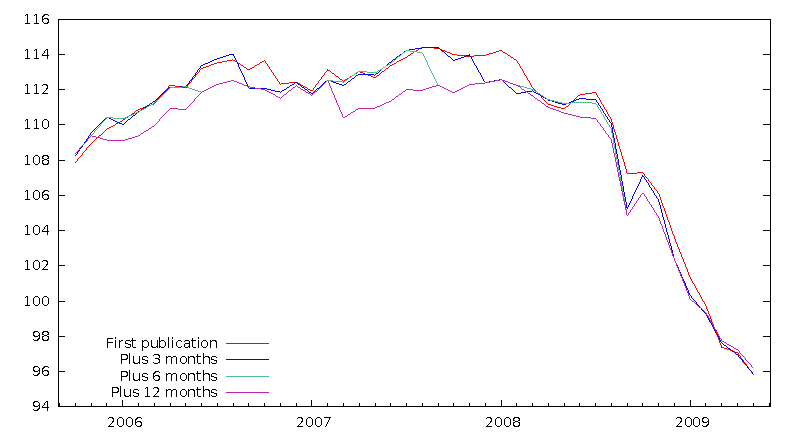
\includegraphics{figures/realtime}
  \caption{Successive revisions to US industrial production}
  \label{fig:realtime-lag}
\end{figure}

\begin{script}[htbp]
  \caption{Retrieving successive realtime lags of US industrial
    production}
  \label{ex:revisions}
\begin{scode}
function series rel_ok (series *obsdate, series *reldate, int p)
  series y_obs, m_obs, y_rel, m_rel, d_rel
  isoconv(obsdate, &y_obs, &m_obs)
  isoconv(reldate, &y_rel, &m_rel, &d_rel)
  series dm = (12*y_rel + m_rel) - (12*y_obs + m_obs)
  return dm < p || (dm == p && d_rel == 1)
end function

nulldata 45
setobs 12 2005:10

string fname = "INDPRO.txt"

# initial published values
join @fname firstpub --data=INDPRO --tkey=observation_date \
--timecols=realtime_start_date --aggr=min(realtime_start_date)

# plus 3 months
join @fname plus3 --data=INDPRO --tkey=observation_date \
--timecols="observation_date,realtime_start_date" \
--filter="rel_ok(&observation_date, &realtime_start_date, 3)" \
--aggr=max(realtime_start_date)

# plus 6 months
join @fname plus6 --data=INDPRO --tkey=observation_date \
--timecols="observation_date,realtime_start_date" \
--filter="rel_ok(&observation_date, &realtime_start_date, 6)" \
--aggr=max(realtime_start_date)

# plus 12 months
join @fname plus12 --data=INDPRO --tkey=observation_date \
--timecols="observation_date,realtime_start_date" \
--filter="rel_ok(&observation_date, &realtime_start_date, 12)" \
--aggr=max(realtime_start_date)

setinfo firstpub --graph-name="First publication"
setinfo plus3 --graph-name="Plus 3 months"
setinfo plus6 --graph-name="Plus 6 months"
setinfo plus12 --graph-name="Plus 12 months"

gnuplot firstpub plus3 plus6 plus12 --time --with-lines \
 --output=realtime.pdf { set key left bottom; }
\end{scode}
\end{script}

\chapter{Funzioni speciali in genr}
\label{chap-genr}

\section{Introduzione}
\label{genr-intro}

Il comando \verb+genr+ offre un modo flessibile per definire nuove
variabili. Il comando � documentato nella \GCR, mentre questo
capitolo offre una discussione pi� approfondita di alcune delle
funzioni speciali disponibili con \verb+genr+ e di alcune
particolarit� del comando.
     
\section{Varianza di lungo periodo}
\label{sec:lrvar}

Come � noto, la varianza della media di $T$ variabili aleatorie
$x_1, x_2, \ldots, x_T$ con uguale varianza $\sigma^2$ � pari a
$\sigma^2/T$ se i dati sono non correlati. In questo caso, la varianza
campionaria di $x_t$ rappresenta uno stimatore consistente.

Se per� esiste correlazione seriale tra le $x_t$, la varianza di
$\bar{X} = T^{-1} \sum_{t=1}^T x_t$ va stimata in modo diverso. Una delle
statistiche pi� usate a questo scopo � uno stimatore kernel non parametrico con
il kernel di Bartlett definito come
\begin{equation}
  \label{eq:scalar-lrvar}
  \hat{\omega}^2(k) = T^{-1} \sum_{t=k}^{T-k} \left[ \sum_{i=-k}^k w_i (x_t -
  \bar{X}) (x_{t-i} - \bar{X}) \right] ,
\end{equation}
dove l'intero $k$ � definito come l'ampiezza della finestra, mentre i termini
$w_i$ sono i cosiddetti \emph{pesi di Bartlett}, definiti come $w_i = 1 -
\frac{|i|}{k + 1}$. Si pu� dimostrare che, per $k$ abbastanza alto,
$\hat{\omega}^2(k)/T$ rappresenta uno stimatore consistente alla varianza di
$\bar{X}$.

\app{Gretl} implementa questo stimatore usando la funzione \texttt{lrvar()}, che
accetta due argomenti: la serie di cui si vuole stimare la varianza di lungo
periodo e lo scalare $k$. Se $k$ � negativo, viene usato il diffuso valore $T^{1/3}$.

\section{Filtri per serie storiche}
\label{sec:filters}

Un tipo di funzioni speciali di \verb+genr+ consente il filtraggio delle serie
storiche. Oltre alle solite operazioni di ritardo e differenza, \app{gretl}
fornisce anche la differenza frazionaria e due filtri usati spesso in
macroeconomia per la scomposizione fra ciclo e trend: il filtro di
Hodrick--Prescott e quello passa banda di Baxter--King.

\subsection{Differenza frazionaria}
\label{sec:fracdiff}

Differenziare una serie storica per $d$ volte � un'operazione ovvia quando
$d$ � un numero intero, ma pu� sembrare strana quando $d$ � una frazione.
Tuttavia, questa idea ha un ben preciso fondamento matematico: si consideri la
funzione
\[
  f(z) = (1 - z)^{-d},
\]
dove $z$ e $d$ sono numeri reali. L'espansione in serie di Taylor intorno a 
$z=0$ mostra che
\[
  f(z) = 1 + dz + \frac{d (d+1)}{2} z^2 + \cdots 
\]
o, pi� sinteticamente,
\[
  f(z) = 1 + \sum_{i=1}^{\infty} \psi_i z^i
\]
con
\[
  \psi_k = \frac{\prod_{i=1}^{k} (d+i-1) }{k!} = \psi_{k-1} \frac{d+k-1}{k}
\]

La stessa espansione pu� essere usata con l'operatore ritardo, cos� che se
definiamo
\[
  Y_t = (1-L)^{0.5} X_t
\]
potrebbe essere considerata equivalente a
\[
Y_t = X_t - 0.5 X_{t-1} - 0.125 X_{t-2} - 0.0625 X_{t-3} - \cdots 
\]
    
In \app{gretl} questa trasformazione pu� essere eseguita con il comando
\begin{code}
genr Y = fracdiff(X,0.5)
\end{code}
    
\subsection{Il filtro di Hodrick--Prescott}
\label{sec:hodrick-prescott}

Questo filtro � utilizzabile tramite la funzione \verb+hpfilt()+, che accetta un
argomento: il nome della variabile da processare.

Una serie storica $y_t$ pu� essere scomposta in un trend, o componente di
crescita $g_t$ e in una componente ciclica $c_t$.  
%
\[
y_t = g_t + c_t, \quad t = 1,2,\dots,T
\]
%
Il filtro di Hodrick--Prescott effettua questa scomposizione, minimizzando
l'espressione seguente:
%
\[
    \sum_{t = 1}^T {(y_t - g_t )^2 } + \lambda \sum_{t = 2}^{T -
      1} \left((g_{t+1} - g_t) - (g_t - g_{t - 1} )\right)^2 .
\]
%
Il primo termine � la somma dei quadrati delle componenti cicliche $c_t =
y_t - g_t$. Il secondo termine � un multiplo $\lambda$ della somma dei quadrati
delle differenze seconde della componente di trend. Questo secondo termine
penalizza le variazioni nel tasso di crescita della componente di trend:
maggiore � il valore di $\lambda$, maggiore sar� la penalizzazione, e quindi pi�
regolare sar� la serie di trend.

Si noti che la funzione \cmd{hpfilt} in \app{gretl} produce la componente di
ciclo, $c_t$, della serie originale. Se si vuole il trend depurato, basta
sottrarre il ciclo dalla serie originale:

\begin{code}
genr ct = hpfilt(yt)
genr gt = yt - ct
\end{code}

Hodrick e Prescott (1997) suggeriscono che un valore $\lambda = 1600$ sia
ragionevole per dati trimestrali. Il valore predefinito in \app{gretl} � il
quadrato della frequenza dei dati, moltiplicato per 100 (che d� appunto 1600 per
dati trimestrali).  Il valore pu� essere modificato con il comando \cmd{set} sul
parametro \cmd{hp\_lambda}.  Ad esempio, \cmd{set hp\_lambda 1200}.

\subsection{Il filtro di Baxter e King}
\label{sec:baxter-king}

Questo filtro � utilizzabile tramite la funzione \verb+bkfilt()+; anche questa
accetta come unico argomento il nome della variabile da processare.

Si consideri la rappresentazione spettrale di una serie storica $y_t$:
%	
\[ y_t = \int_{-\pi}^{\pi} e^{i\omega} \mathrm{d} Z(\omega) \]
%
Per estrarre la componente di $y_t$ che si trova tra le frequenze
$\underline{\omega}$ e $\overline{\omega}$ potremmo applicare un filtro passa
banda:
%	
\[ c^*_t = \int_{-\pi}^{\pi} F^*(\omega) e^{i\omega} \mathrm{d}
Z(\omega) \] 
%
dove $F^*(\omega) = 1$ per $\underline{\omega} < |\omega| <
\overline{\omega}$ e 0 altrove. Ci� implicherebbe, nel dominio
temporale, applicare alla serie un filtro con un numero infinito di
coefficienti, cosa non desiderabile. Il filtro passa banda di Baxter e
King applica a $y_t$ un polinomio finito nell'operatore di ritardo
$A(L)$:
%	
\[ c_t = A(L) y_t \]
%
dove $A$($L$) � definito come
%	
\[ A(L) = \sum_{i=-k}^{k} a_i L^i \]

I coefficienti $a_i$ sono scelti in modo che $F(\omega) =
A(e^{i\omega})A(e^{-i\omega})$ sia la migliore approssimazione di
$F^*(\omega)$ per un dato $k$. Chiaramente, maggiore � $k$, migliore �
l'approssimazione, ma poich� ci� implica scartare $2k$ osservazioni, di
solito si cerca un compromesso.  Inoltre, il filtro ha altre propriet�
teoriche interessanti, tra cui quella che $a(1) = 0$, quindi una serie
con una sola radice unitaria � resa stazionaria dall'applicazione del
filtro.

In pratica, il filtro � usato di solito con dati mensili o trimestrali
per estrarne la componente di ``ciclo economico'', ossia la componente
tra 6 e 36 trimestri. I valori usuali per $k$ sono 8 o 12 (o forse di
pi� per serie mensili).  I valori predefiniti per i limiti di
frequenza sono 8 e 32, mentre il valore predefinito per l'ordine di
approssimazione, $k$, � 8.  � possibile impostare questi valori usando
il comando \cmd{set}.  La parola chiave per impostare i limiti di
frequenza � \verb+bkbp_limits+, mentre quella per $k$ � \verb+bkbp_k+.
Quindi ad esempio, se si stanno usando dati mensili e si vuole
impostare i limiti di frequenza tra 18 e 96, e $k$ a 24, si pu�
eseguire

\begin{code}
set bkbp_limits 18 96
set bkbp_k 24
\end{code}

Questi valori resteranno in vigore per le chiamate alla funzione
\verb+bkfilt+ finch� non saranno modificati da un altro uso di
\verb+set+.

\section{Dati panel}
\label{panel-genr}

\subsection{Variabili dummy}
\label{dummies}

In uno studio panel, pu� nascere l'esigenza di costruire delle
variabili dummy di uno dei seguenti tipi: (a) dummy che identificano
ciascuna delle unit� cross-section, o (b) dummy che identificano
ciascuno dei periodi. Il primo tipo pu� essere usato per
permettere all'intercetta della regressione di variare tra le unit�
cross-section, il secondo per permettere all'intercetta di variare tra
i periodi.

Per creare questo tipo di dummy, � possibile usare le due funzioni
speciali del men� \textsf{Aggiungi}, o del comando testuale \cmd{genr}.

\begin{enumerate}
\item ``Dummy per unit�'' (comando testuale \cmd{genr unitdum}).
  Questo comando crea un insieme di variabili dummy che identificano
  le unit� cross section.  La variabile \verb+du_1+ avr� valore 1 in
  ogni riga dei dati che corrisponde a un'osservazione della prima
  unit� cross section, e 0 altrove; \verb+du_2+ avr� valore 1 in ogni
  riga dei dati che corrisponde a un'osservazione della seconda unit�
  cross section, e cos� via.
        
\item ``Dummy temporali'' (comando testuale \cmd{genr timedum}).
  Questo comando crea un insieme di variabili dummy che identificano
  i periodi.  La variabile \verb+dt_1+ avr� valore 1 in ogni riga dei dati che
  corrisponde a un'osservazione del primo periodo, e 0 altrove; \verb+dt_2+ avr�
  valore 1 in ogni riga dei dati che corrisponde a un'osservazione del secondo
  periodo, e cos� via.

\end{enumerate}

Se un dataset panel contiene l'anno di ogni osservazione all'interno
della variabile \verb+ANNO+, � possibile creare una dummy periodica
per un anno particolare, ad esempio con \cmd{genr dum = (ANNO=1960)}.
� anche possibile creare variabili dummy periodiche usando l'operatore
modulo, \verb+%+.  Ad esempio, per creare una dummy che
valga 1 ogni trenta osservazioni a partire dalla prima e 0 altrove,
basta eseguire
%
\begin{code}
genr index 
genr dum = ((index-1)%30) = 0
\end{code}



\subsection{Ritardi, differenze, trend}
\label{panel-lagged}

Se i periodi temporali sono distanziati in modo uniforme, � possibile
usare valori ritardati delle variabili in una regressione panel (ma si
veda la sezione~\ref{panel-dyn}; � anche possibile costruire
differenze prime delle variabili.

Se un dataset � identificato correttamente come panel,  \app{gretl}
gestir� correttamente la generazione di questo tipo di variabili. Ad
esempio, il comando \verb+genr x1_1 = x1(-1)+ creer� una variabile che
contiene il primo ritardo di \verb+x1+, laddove � disponibile, e il
codice di valore mancante, laddove il ritardo non � disponibile (ad esempio
nella prima osservazione per ogni gruppo).  Quando si esegue una regressione che
include questo tipo di variabili, il programma escluder� automaticamente le
osservazioni mancanti.

Quando un dataset panel ha una dimensione temporale sostanziale, pu� essere
utile includere un trend nell'analisi. Il comando \cmd{genr time} 
crea una variabile di nome \varname{time} che assume valori compresi tra 1 e $T$
per ogni unit�, dove $T$ � la lunghezza della dimensione temporale del panel.
Per creare un indice che assuma valori compresi tra 1 e $m\times T$, dove $m$
� il numero di unit� nel panel, si usi invece \cmd{genr index}.

\subsection{Statistiche descrittive per unit�}
\label{panel-stats}

Le funzioni \texttt{pmean()} e \texttt{psd()} possono essere usate per generare
semplici statistiche descrittive (media e scarto quadratico medio) per una data
variabile, calcolate per gruppo.

Supponendo di avere un dataset panel che comprende 8 osservazioni temporali per
ciascuna di $N$ unit� o gruppi. Il comando
%
\begin{code}
genr pmx = pmean(x)
\end{code}
%
crea una serie di questo tipo: i primi 8 valori (che corrispondono all'unit� 1)
contengono la media di \varname{x} per l'unit� 1, i successivi 8 valori
contengono la media per l'unit� 2 e cos� via. La funzione \texttt{psd()}
funziona in modo simile. Lo scarto quadratico medio campionario per il gruppo
$i$ � calcolato come
\[
s_i = \sqrt{\frac{\sum(x-\bar{x}_i)^2}{T_i-1}}
\]
dove $T_i$ denota il numero di osservazioni valide su \varname{x}
per l'unit� data, $\bar{x}_i$ denota la media di gruppo, e la somma viene fatta
su tutte le osservazioni valide per il gruppo. Se per� vale $T_i < 2$,
lo scarto quadratico medio viene impostato pari a 0.

� interessante notare un uso particolare di \texttt{psd()}: se si vuole formare
un sotto-campione di un panel che contenga solo quelle unit� per cui la
variabile \varname{x} varia nel tempo, si pu� eseguire
%
\begin{code}
smpl (psd(x) > 0) --restrict
\end{code}

\subsection{Funzioni speciali per manipolare i dati}
\label{panel-manip}

Oltre alle funzioni discusse sopra, ci sono alcune opzioni di \texttt{genr}
particolarmente utili per manipolare i dati panel, soprattutto quando i dati
sono stati importati da una fonte esterna e non sono nella forma corretta per
l'analisi panel. Queste funzionalit� sono spiegate nel Capitolo~\ref{datafiles}.


\section{Ricampionamento e bootstrapping}
\label{sec:genr-resample}

Un'altra funzione particolare � il ricampionamento, con reimmissione,
di una serie. Data una serie di dati originale \varname{x}, il comando
%
\begin{code}
genr xr = resample(x)
\end{code}
%
crea una nuova serie in cui ognuno degli elementi � estratto in modo casuale
dagli elementi di \varname{x}. Se la serie originale ha 100 osservazioni, ogni
elemento di \varname{x} � scelto con probabilit� $1/100$ ad ogni estrazione.
L'effetto � quindi di ``rimescolare'' gli elementi di \varname{x}, con la
particolarit� che ogni elemento di \varname{x} pu� apparire pi� di una volta, o
non apparire affatto, in \varname{xr}.

L'uso principale di questa funzione � la costruzione di intervalli di confidenza
o p-value con il metodo bootstrap. Ecco un semplice esempio: si supponga di aver
stimato una semplice regressione OLS di $y$ su $x$ e di aver trovato che il
coefficiente della pendenza abbia un rapporto $t$ pari a 2.5 con 40 gradi di
libert�.  Il p-value a due code per l'ipotesi nulla che il parametro della
pendenza sia pari a zero vale quindi 0.0166, usando la distribuzione $t(40)$. A
seconda del contesto, per�, potremmo dubitare del fatto che il rapporto tra il
coefficiente e l'errore standard segua veramente una distribuzione $t(40)$. In
questo caso, potremmo derivare un valore bootstrap per il p-value come mostrato
nell'esempio~\ref{resampling-loop}.  

Sotto l'ipotesi nulla che la pendenza rispetto a $x$ sia pari a zero,
$y$ � uguale alla sua media pi� un termine di errore. Simuliamo $y$
ricampionando i residui del modello OLS iniziale e ri-stimiamo il modello.
Ripetiamo questa procedura un gran numero di volte e registriamo il numero di
casi in cui il valore assoluto del rapporto $t$ � maggiore di 2.5: la
proporzione di questo numero di casi � il nostro valore bootstrap per il
p-value. Per una buona discussione dei test basati sulla simulazione e sui
metodi bootstrap, si veda Davidson e MacKinnon (2004, capitolo 4).

\begin{script}[htbp]
  \caption{Calcolo del p-value col metodo bootstrap}
  \label{resampling-loop}
\begin{scode}
ols y 0 x
# salva i residui
genr ui = $uhat
scalar ybar = mean(y)
# numero delle replicazioni per il bootstrap
scalar replics = 10000
scalar tcount = 0
series ysim = 0
loop replics --quiet
  # genera i valori simulati di y ricampionando
  ysim = ybar + resample(ui)
  ols ysim 0 x
  scalar tsim = abs($coeff(x) / $stderr(x))
  tcount += (tsim > 2.5)
endloop      
printf "Proporzione dei casi con |t| > 2.5 = %g\n", tcount / replics
\end{scode}
%$
\end{script}
   

\section{Densit� cumulate e p-value}
\label{sec:genr-cdf}

Le due funzioni \cmd{cdf} e \cmd{pvalue} forniscono strumenti complementari per
esaminare i valori di varie distribuzioni di probabilit�: la normale standard,
la $t$ di Student, la $\chi^2$, la $F$, la gamma, e la binomiale.
La sintassi di queste funzioni � spiegata nella \GCR; in questa sede viene
presentato un aspetto particolare riguardante la precisione dei risultati.

La funzione di ripartizione, o di densit� cumulata (CDF), per una variabile
casuale � l'integrale della densit� della variabile, dal suo limite inferiore
(tipicamente $-\infty$ o 0) fino a un certo valore $x$. Il p-value (almeno il
p-value destro, a una coda, fornito dalla funzione \cmd{pvalue}) � la
probabilit� complementare, l'integrale da $x$ al limite superiore della
distribuzione, tipicamente $+\infty$.  

In linea di principio non c'� bisogno di due funzioni distinte: dato un valore
della funzione di ripartizione $p_0$ � possibile ricavare facilmente il p-value
come $1-p_0$ (o viceversa).  In pratica, poich� il computer usa aritmetica a
precisione finita, due funzioni non sono ridondanti. In \app{gretl}, come nella
maggior parte dei programmi statistici, i numeri a virgola mobile sono
rappresentati tramite dei ``double'' --- valori a precisione doppia, che sono
tipicamente memorizzati in 8 byte, o 64 bit. Visto che il numero di bit
disponibili � fisso, i numeri in virgola mobile che possono essere rappresentati
sono limitati: \textit{i ``double'' non modellano esattamente la retta reale}.
Tipicamente, i ``double'' possono rappresentare numeri che stanno all'incirca
nell'intervallo $\pm 1.7977 \times 10^{308}$, ma con circa solo 15 cifre di
precisione.

Supponiamo di essere interessati alla coda sinistra della distribuzione $\chi^2$
con 50 gradi di libert�, ossia di voler conoscere il valore della CDF per $x =
0.9$.  Vediamo la seguente sessione interattiva:
\begin{code}
? genr p1 = cdf(X, 50, 0.9)
Generato lo scalare p1 (ID 2) = 8.94977e-35
? genr p2 = pvalue(X, 50, 0.9)
Generato lo scalare p2 (ID 3) = 1
? genr test = 1 - p2
Generato lo scalare test (ID 4) = 0
\end{code}

La funzione \cmd{cdf} ha prodotto un valore accurato, ma la funzione
\cmd{pvalue} ha dato come risultato 1, da cui non � possibile ricavare il valore
della CDF. Questo pu� sembrare sorprendente, ma si spiega considerando che se il
valore di \texttt{p1} � corretto, il valore corretto di \texttt{p2} � $1 -
8.94977 \times 10^{-35}$, ma non c'� modo di rappresentare questo valore con un
``double'': richiederebbe oltre 30 cifre di precisione.

Ovviamente questo � un esempio estremo. Se il valore di $x$ in questione non si
trova alle estremit� di una delle due code della distribuzione, le funzioni
\cmd{cdf} e \cmd{pvalue} produrranno risultati complementari, come si vede da
questo esempio:
\begin{code}
? genr p1 = cdf(X, 50, 30)
Generato lo scalare p1 (ID 2) = 0.0111648
? genr p2 = pvalue(X, 50, 30)
Generato lo scalare p2 (ID 3) = 0.988835
? genr test = 1 - p2
Generato lo scalare test (ID 4) = 0.0111648
\end{code}
La morale � che se occorre esaminare valori estremi, occorre scegliere
attentamente la funzione da usare, tenendo presente che valori molto vicini allo
zero possono essere rappresentati con ``double'', mentre valori molto vicini a 1
possono non esserlo.

\section{Gestione dei valori mancanti}
\label{sec:genr-missing}

Sono disponibili quattro funzioni speciali per gestire i valori
mancanti.  La funzione booleana \verb+missing()+ richiede come unico
argomento il nome di una variabile e produce una serie con valore 1
per ogni osservazione in cui la variabile indicata ha un valore
mancante, 0 altrove (ossia dove la variabile indicata ha un valore
valido). La funzione \verb+ok()+ � il complemento di \verb+missing+,
ossia una scorciatoia per \verb+!missing+ (dove \verb+!+ � l'operatore
booleano NOT).  Ad esempio, � possibile contare i valori mancanti
della variabile \verb+x+ usando

\begin{code}
genr nmanc_x = sum(missing(x))
\end{code}

La funzione \verb+zeromiss()+, che richiede anch'essa come unico
argomento il nome di una serie, produce una serie in cui tutti i
valori zero sono trasformati in valori mancanti. Occorre usarla con
attenzione (di solito non bisogna confondere valori mancanti col
valore zero), ma pu� essere utile in alcuni casi: ad esempio, �
possibile determinare la prima osservazione valida di una variabile
\verb+x+ usando

\begin{code}
genr time
genr x0 = min(zeromiss(time * ok(x)))
\end{code}


La funzione \verb+misszero()+ compie l'operazione opposta di
\verb+zeromiss+, ossia converte tutti i valori mancanti in zero.  

Pu� essere utile chiarire la propagazione dei valori mancanti
all'interno delle formule di \verb+genr+. La regola generale � che
nelle operazioni aritmetiche che coinvolgono due variabili, se una
delle variabili ha un valore mancante in corrispondenza
dell'osservazione $t$, anche la serie risultante avr� un valore
mancante in $t$. L'unica eccezione a questa regola � la
moltiplicazione per zero: zero moltiplicato per un valore mancante
produce sempre zero (visto che matematicamente il risultato � zero a
prescindere dal valore dell'altro fattore).
    

\section{Recupero di variabili interne}
\label{sec:genr-internal}

Il comando \verb+genr+ fornisce un modo per recuperare vari valori
calcolati dal programma nel corso della stima dei modelli o della
verifica di ipotesi. Le variabili che possono essere richiamate in
questo modo sono elencate nella \GCR; qui ci occupiamo in particolare
delle variabili speciali \verb+$test+ e \verb+$pvalue+.

Queste variabili contengono, rispettivamente, il valore dell'ultima
statistica test calcolata durante l'ultimo uso esplicito di un comando
di test e il p-value per quella statistica test. Se non � stato
eseguito alcun comando di test, le variabili contengono il codice di
valore mancante. I ``comandi espliciti di test'' che funzionano in
questo modo sono i seguenti: \cmd{add} (test congiunto per la
significativit� di variabili aggiunte a un modello); \cmd{adf} (test
di Dickey--Fuller aumentato, si veda oltre); \cmd{arch} (test per
ARCH); \cmd{chow} (test Chow per break strutturale); \cmd{coeffsum}
(test per la somma dei coefficienti specificati); \cmd{cusum}
(statistica \emph{t} di Harvey--Collier); \cmd{kpss} (test di
stazionariet� KPSS, p-value non disponibile); \cmd{lmtest} (si veda
oltre); \cmd{meantest} (test per la differenza delle medie);
\cmd{omit} (test congiunto per la significativit� delle variabili
omesse da un modello); \cmd{reset} (test RESET di Ramsey);
\cmd{restrict} (vincolo lineare generale); \cmd{runs} (test delle
successioni per la casualit�); \cmd{testuhat} (test per la normalit�
dei residui) e \cmd{vartest} (test per la differenza delle varianze).
Nella maggior parte dei casi, vengono salvati valori sia in
\verb+$test+ che in \verb+$pvalue+; l'eccezione � il test KPSS, per
cui non � disponibile il p-value.
    
Un punto da tenere in considerazione a questo proposito � che le
variabili interne \verb+$test+ e \verb+$pvalue+ vengono sovrascritte
ogni volta che viene eseguito uno dei test elencati sopra. Se si
intende referenziare questi valori durante una sequenza di comandi
\app{gretl}, occorre farlo nel momento giusto.
    
Un'altra questione � data dal fatto che alcuni dei comandi di test di
solito generano pi� di una statistica test e pi� di un p-value: in questi casi
vengono salvati solo gli ultimi valori. Per controllare in modo
preciso quali valori vengono recuperati da \verb+$test+ e
\verb+$pvalue+ occorre formulare il comando di test in modo che il
risultato non sia ambiguo. Questa nota vale in particolare per i
comandi \verb+adf+ e \verb+lmtest+.

\begin{itemize}
\item Di solito, il comando \cmd{adf} genera tre varianti del test
  Dickey--Fuller: una basata su una regressione che include una
  costante, una che include costante e trend lineare, e una che
  include costante e trend quadratico. Se si intende estrarre valori
  da \verb+$test+ o \verb+$pvalue+ dopo aver usato questo comando, �
  possibile selezionare la variante per cui verranno salvati i valori,
  usando una delle opzioni \verb+--nc+, \verb+--c+, \verb+--ct+ o
  \verb+--ctt+ con il comando \verb+adf+.
\item Di solito, il comando \cmd{lmtest} (che deve seguire una
  regressione OLS) esegue vari test diagnostici sulla regressione in
  questione. Per controllare cosa viene salvato in \verb+$test+ e
  \verb+$pvalue+ occorre limitare il test usando una delle opzioni
  \verb+--logs+, \verb+--autocorr+, \verb+--squares+ 
  o \verb+--white+.
\end{itemize}

Un aspetto comodo per l'uso dei valori immagazzinati in \verb+$test+ e
\verb+$pvalue+ � dato dal fatto che il tipo di test a cui si
riferiscono questi valori viene scritto nell'etichetta descrittiva
della variabile generata. Per controllare di aver recuperato il valore
corretto, � possibile leggere l'etichetta con il comando \cmd{label}
(il cui unico argomento � il nome della variabile). La seguente
sessione interattiva illustra la procedura.
    
\begin{code}
? adf 4 x1 --c
Test Dickey-Fuller aumentati, ordine 4, per x1
ampiezza campionaria 59
ipotesi nulla di radice unitaria: a = 1
  test con costante
  modello: (1 - L)y = b0 + (a-1)*y(-1) + ... + e
  valore stimato di (a - 1): -0.216889
  statistica test: t = -1.83491
  p-value asintotico 0.3638
P-value basati su MacKinnon (JAE, 1996)
? genr pv = $pvalue
Generato lo scalare pv (ID 13) = 0.363844
? label pv    
  pv=Dickey-Fuller pvalue (scalar)
\end{code}
%$

\section{Procedure numeriche}
\label{sec:genr-numerical}

Esistono due funzioni particolarmente utili per costruire stimatori speciali,
ossia \texttt{BFGSmax} (il massimizzatore BFGS, discusso nel Capitolo~\ref{chap:mle})
e \texttt{fdjac}, che produce un'approssimazione del Jacobiano calcolata col
metodo della differenza finita in avanti.

\subsection{Il massimizzatore BFGS}
\label{sec:BFGSmax}

La funzione \texttt{BFGSmax} accetta due argomenti: un vettore che contiene i
valori iniziali di un insieme di parametri, e una stringa che specifica una
chiamata a una funzione che calcola il criterio (scalare) da massimizzare, dati
i valori attuali dei parametri e gli altri dati rilevanti.
Se si tratta di una minimizzazione, questa funzione dovrebbe produrre il
criterio con segno negativo. In caso di successo, \texttt{BFGSmax}
produce il valore massimo del criterio e la matrice indicata come primo
argomento contiene i valori dei parametri che producono il massimo. Ecco un
esempio:
%
\begin{code}
matrix X = { dataset }
matrix theta = { 1, 100 }'
scalar J = BFGSmax(theta, "Funzione(&theta, &X)")
\end{code}
%
Si assume che \texttt{Funzione} sia una funzione definita dall'utente
(si veda il Capitolo~\ref{chap:functions}) con una struttura di questo tipo:
%
\begin{code}
function Funzione (matrix *theta, matrix *X)
  scalar val = ...  # Esegue dei calcoli
  return scalar val
end function
\end{code}

\begin{script}[htbp]
  \caption{Ricerca del minimo della funzione di Rosenbrock}
  \label{rosenbrock}
\begin{scode}
function Rosenbrock(matrix *param)
  scalar x = param[1]
  scalar y = param[2]
  scalar f = -(1-x)^2 - 100 * (y - x^2)^2
  return scalar f 
end function

nulldata 10

matrix theta = { 0 , 0 }

set max_verbose 1
M = BFGSmax(theta, "Rosenbrock(&theta)")

print theta
\end{scode}
\end{script}

Il funzionamento del massimizzatore BFGS pu� essere regolato usando il comando
\texttt{set} sulle variabili \verb+bfgs_maxiter+ e \verb+bfgs_toler+ (si veda
il Capitolo~\ref{chap:mle}). Inoltre, � possibile vedere i dettagli della
massimizzazione assegnando un valore positivo alla variabile
\verb|max_verbose|, sempre con il comando \texttt{set}.

Spesso, per testare gli algoritmi di ottimizzazione si usa la funzione di
Rosenbrock, chiamata anche ``valle di Rosenbrock'' o la ``funzione a banana di
Rosenbrock'', visto che le linee di contorno sono a forma di banana. Questa �
definita come:
%
\[
    f(x,y) = (1 - x)^2 + 100(y - x^2)^2
\]
%
La funzione ha un minimo globale in $(x,y) = (1,1)$ dove vale $f(x,y) = 0$.
L'Esempio~\ref{rosenbrock} mostra uno script di \app{gretl} che cerca il minimo
usando la funzione \texttt{BFGSmax} (mostrando i dettagli sul progresso del
calcolo).

\subsection{Calcolo di un Jacobiano}
\label{sec:fdjac}

\app{Gretl} offre la possibilit� di differenziare numericamente una funzione
definita dall'utente, usando la funzione \texttt{fdjac}.

Questa funzione accetta due argomenti: una matrice $n \times 1$
che contiene i valori iniziali dei parametri e una stringa che specifica una
chiamata a una funzione che calcola e produce una matrice $m \times 1$,
dati i valori attuali dei parametri e gli altri dati rilevanti.
In caso di successo, viene prodotta una matrice $m \times n$ che contiene il
Jacobiano. Ad esempio,
%
\begin{code}
matrix Jac = fdjac(theta, "Somma(&theta, &X)")
\end{code}
dove si assume che \texttt{Somma} sia una funzione definita dall'utente con la
struttura seguente:
%
\begin{code}
function Somma (matrix *theta, matrix *X)
  matrix V = ...  # Esegue dei calcoli
  return matrix V
end function
\end{code}

Questo pu� rivelarsi utile in vari casi: ad esempio, se si usa
\texttt{BFGSmax} per stimare un modello, si potrebbe voler calcolare
un'approssimazione numerica al Jacobiano rilevante per costruire una matrice di
covarianza per le stime.

Un altro esempio � rappresentato dal metodo delta: se si ha uno stimatore
consistente di un vettore di parametri $\hat{\theta}$ e una stima consistente
della sua matrice di covarianza $\Sigma$, potrebbe essere necessario calcolare
stime di una trasformazione nonlineare continua $\psi = g(\theta)$. In questo caso,
un risultato standard della teoria asintotica � il seguente:
\[
\left\{
    \begin{array}{c}
      \hat{\theta} \convp \theta \\ 
      \sqrt{T} \left( \hat{\theta} - \theta \right) \convd N(0, \Sigma)
    \end{array}
\right\}
    \Longrightarrow
\left\{
    \begin{array}{c}
      \hat{\psi} = g(\hat{\theta}) \convp \psi = g(\theta) \\ 
      \sqrt{T} \left( \hat{\psi} - \psi \right) \convd N(0, J
      \Sigma J')
    \end{array}
\right\}
\]
dove $T$ � l'ampiezza del campione, mentre $J$ � il Jacobiano
$\left.\pder{\psi}{\theta}\right|_{\theta = \hat{\theta}}$.

\begin{script}[htbp]
  \caption{Metodo delta}
  \label{delta-method}
\begin{scode}
function MPC(matrix *param, matrix *Y)
  beta = param[2]
  gamma = param[3]
  y = Y[1]
  matrix ret = beta*gamma*y^(gamma-1)
  return matrix ret
end function

# William Greene, Econometric Analysis, 5e, Chapter 9
set echo off
set messages off
open greene5_1.gdt

# Usa OLS per inizializzare i parametri
ols realcons 0 realdpi --quiet
genr a = $coeff(0)
genr b = $coeff(realdpi)
genr g = 1.0

# Esegui NLS con derivate analitiche
nls realcons = a + b * (realdpi^g)
  deriv a = 1
  deriv b = realdpi^g
  deriv g = b * realdpi^g * log(realdpi)
end nls

matrix Y = realdpi[2000:4]
matrix theta = $coeff
matrix V = $vcv

mpc = MPC(&theta, &Y)
matrix Jac = fdjac(theta, "MPC(&theta, &Y)")
Sigma = qform(Jac, V)

printf "\nmpc = %g, std.err = %g\n", mpc, sqrt(Sigma)
scalar teststat = (mpc-1)/sqrt(Sigma)
printf "\nTest per MPC = 1: %g (p-value = %g)\n", \
	teststat, pvalue(n,abs(teststat))
\end{scode}
\end{script}

Lo script \ref{delta-method} esemplifica questo caso: � tratto da Greene (2003),
sezione 9.3.1. Le leggere differenze tra i risultati riportati nel testo
originale e quelli prodotti da \app{gretl} sono dovuti al fatto che il Jacobiano
� calcolato numericamente, invece che analiticamente come nel testo.

\section{La trasformata discreta di Fourier}
\label{sec:genr-fft}

La trasformata discreta di Fourier � una trasformazione lineare invertibile
di un vettore complesso. Quindi, se $\mathbf{x}$ � un vettore
$n$-dimensionale il cui $k$-esimo elemento � $x_k = a_k + i b_k$, il risultato
della trasformata discreta di Fourier � un vettore
$\mathbf{f} = \mathcal{F}(\mathbf{x})$ il cui $k$-esimo elemento �
\[
  f_k = \sum_{j=0}^{n-1} e^{-i \omega_{j,k} } x_j 
\]
dove $\omega_{j,k} = 2 \pi i \frac{j k}{n}$. Poich� la trasformazione
� invertibile, il vettore $\mathbf{x}$ pu� essere ricavato da
$\mathbf{f}$ usando la cosidetta trasformata inversa
\[
  x_k = \frac{1}{n} \sum_{j=0}^{n-1} e^{i \omega_{j,k} } f_j .
\]

La trasformata di Fourier � usata in varie situazioni, grazie a questa sua
propriet� fondamentale: la convoluzione di due vettori pu� essere calcolata in
modo efficiente moltiplicando gli elementi delle loro trasformate di Fourier e
invertendo il risultato. Se
\[
  z_k = \sum_{j=1}^n x_j y_{k-j} ,
\]
allora vale
\[
  \mathcal{F}(\mathbf{z}) = \mathcal{F}(\mathbf{x}) \odot
  \mathcal{F}(\mathbf{y}) .
\]
Ossia, $\mathcal{F}(\mathbf{z})_k = \mathcal{F}(\mathbf{x})_k
\mathcal{F}(\mathbf{y})_k$.

Per calcolare la trasformata di Fourier, \app{gretl} usa la libreria esterna
\texttt{fftw3} (si veda Frigo e Johnson 2003), che garantisce velocit� e
accuratezza estreme. Infatti il tempo di processore necessario a compiere la
trasformazione � $O(n \log n)$ per ogni $n$. Ecco perch� l'insieme di tecniche
numeriche impiegate in \texttt{fftw3} � chiamato comunemente Trasformata
\emph{Veloce} di Fourier.

\app{Gretl} fornisce due funzioni matriciali\footnote{Si veda il capitolo
  \ref{chap:matrices}.} per calcolare la trasformata di Fourier e la sua
inversa: \texttt{fft} e   \texttt{ffti}. In realt� l'implementazione della
trasformata di Fourier di \app{gretl} � un po' pi� specializzata: il valore di
ingresso della funzione \texttt{fft} deve essere reale. Al contrario,
\texttt{ffti} richiede un argomento complesso e produce un risultato reale. Ad
esempio:
\begin{code}
x1 = { 1 ; 2 ; 3 }
# Esegue la trasformazione
f = fft(a)
# Esegue la trasformazione inversa
x2 = ffti(f)
\end{code}
produce
\[
  x_1 = \left[ \begin{array}{c} 1 \\ 2 \\ 3 \end{array} \right] 
  \qquad
  f = \left[ \begin{array}{rr} 
      6 & 0 \\ -1.5 & 0.866 \\ -1.5 & -0.866 
   \end{array} \right] 
  \qquad
  x_2 = \left[ \begin{array}{c} 1 \\ 2 \\ 3 \end{array} \right] 
\]
dove la prima colonna di \emph{f} contiene la parte reale, mentre la seconda la
parte complessa. In generale, se l'argomento di \texttt{fft} ha
$n$ colonne, il risultato ne ha $2n$, dove le parti reali sono contenute
nelle colonne dispari, mentre le parti complesse in quelle pari. Se fosse
necessario calcolare la trasformata di Fourier su molti vettori con lo stesso
numero di elementi, � numericamente pi� efficiente raggrupparli in una matrice,
piuttosto che eseguire \texttt{fft} separatamente per ogni vettore.

Ad esempio, si consideri la moltiplicazione di due polinomi:
\begin{eqnarray*}
  a(x) & = & 1 + 0.5 x \\
  b(x) & = & 1 + 0.3 x - 0.8 x^2 \\
  c(x) = a(x) \cdot b(x) & = & 1 + 0.8 x - 0.65 x^2 - 0.4 x^3
\end{eqnarray*}
I coefficienti del polinomio $c(x)$ sono la convoluzione dei coefficienti di
$a(x)$ e $b(x)$; il seguente codice per \app{gretl} illustra come calcolare i
coefficienti di $c(x)$:
\begin{code}
# Definizione dei due polinomi
a = { 1, 0.5, 0, 0 }'
b = { 1, 0.3, -0.8, 0 }'
# Calcolo delle trasformate
fa = fft(a)
fb = fft(b)
# Moltiplicazione complessa delle due trasformate
fc = cmult(fa, fb)
# Calcolo dei coefficienti di c usando la trasformata inversa
c = ffti(fc)
\end{code}

L'efficienza massima si otterrebbe raggruppando \texttt{a} e
\texttt{b} in una matrice. Il vantaggio computazionale nell'esempio appena visto
� trascurabile, ma nel caso di un gran numero di righe o colonne, � preferibile
procedere nel modo seguente:
\begin{code}
# Definizione dei due polinomi
a = { 1 ; 0.5; 0 ; 0 }
b = { 1 ; 0.3 ; -0.8 ; 0 }
# Calcolo congiunto delle trasformate
f = fft(a ~ b)
# Moltiplicazione complessa delle due trasformate
fc = cmult(f[,1:2], f[,3:4])
# Calcolo dei coefficienti di c usando la trasformata inversa
c = ffti(fc)
\end{code}

In econometria la trasformata di Fourier � usata per lo pi� nell'analisi delle
serie storiche, ad esempio nel calcolo del periodogramma. Lo script
\ref{scr:pergm-fft} mostra come calcolare il periodogramma di una serie storica
usando la funzione \texttt{fft}.

\begin{script}[htbp]
  \caption{Periodogramma usando la trasformata di Fourier}
  \label{scr:pergm-fft}
\begin{scode}
nulldata 50
# Genera un processo AR(1)
series e = normal()
series x = 0
x = 0.9*x(-1) + e
# Calcola il periodogramma
scale = 2*pi*$nobs
X = { x }
F = fft(X)
S = sumr(F.^2)
S = S[2:($nobs/2)+1]/scale
omega = seq(1,($nobs/2))' .* (2*pi/$nobs)
omega = omega ~ S
# Confronto con il comando pergm
pergm x  
print omega
\end{scode}
\end{script}


%%% Local Variables: 
%%% mode: latex
%%% TeX-master: "gretl-guide-it"
%%% End: 


\chapter{Gretl data types}
\label{chap:datatypes}

\section{Introduction}

Gretl offers the following data types:
%
\begin{center}
\begin{tabular}{lp{.8\textwidth}}
\texttt{scalar} & holds a single numerical value\\
\texttt{series} & holds $n$ numerical values, where $n$
 is the number of observations in the current dataset \\
\texttt{matrix} & holds a rectangular array of numerical
 values, of any dimensions\\
\texttt{list} & holds the ID numbers of a set of series \\
\texttt{string} & holds an array of characters\\
\texttt{bundle} & holds a variable number of objects of 
 various types \\
\texttt{array} & holds a variable number of objects of 
 a given type
\end{tabular}
\end{center}

The ``numerical values'' mentioned above are all double-precision
floating point numbers.

In this chapter we give a run-down of the basic characteristics of
each of these types and also explain their ``life cycle'' (creation,
modification and destruction). The list and matrix types, whose uses
are relatively complex, are discussed at greater length in the
following two chapters. 

\section{Series}
\label{sec:Series}

We begin with the \texttt{series} type, which is the oldest and in a
sense the most basic type in gretl. When you open a data file in the
gretl GUI, what you see in the main window are the ID numbers, names
(and descriptions, if available) of the series read from the file. All
the series existing at any point in a gretl session are of the same
length, although some may have missing values. The variables that can
be added via the items under the \textsf{Add} menu in the main window
(logs, squares and so on) are also series.

For a gretl session to contain any series, a common series length must
be established. This is usually achieved by opening a data file, or
importing a series from a database, in which case the length is set by
the first import. But one can also use the \texttt{nulldata} command,
which takes as it single argument the desired length, a positive
integer.

Each series has these basic attributes: an ID number, a name, and of
course $n$ numerical values. In addition a series may have a
description (which is shown in the main window and is also accessible
via the \texttt{labels} command), a ``display name'' for use in
graphs, a record of the compaction method used in reducing the
variable's frequency (for time-series data only) and a flag marking
the variable as discrete. These attributes can be edited in the GUI by
choosing \textsf{Edit Attributes} (either under the \textsf{Variable}
menu or via right-click), or by means of the \texttt{setinfo} command.

In the context of most commands you are able to reference series by
name or by ID number as you wish. The main exception is the definition
or modification of variables via a formula; here you must use names
since ID numbers would get confused with numerical constants.

Note that series ID numbers are always consecutive, and the ID number
for a given series will change if you delete a lower-numbered series.
In some contexts, where gretl is liable to get confused by such
changes, deletion of low-numbered series is disallowed.

\subsection{Discrete series}

It is possible to mark variables of the series type as
\textit{discrete}. The meaning and uses of this facility are explained
in chapter~\ref{chap:discrete}.


\section{Scalars}
\label{sec:Scalars}

The scalar type is relatively simple: just a convenient named holder
for a single numerical value. Scalars have none of the additional
attributes pertaining to series, do not have ID numbers, and must be
referenced by name. A common use of scalar variables is to record
information made available by gretl commands for further processing,
as in \texttt{scalar s2 = \$sigma\^{}2} to record the square of the
standard error of the regression following an estimation command such
as \texttt{ols}.

You can define and work with scalars in gretl without having any
dataset in place.

In the gretl GUI, scalar variables can be inspected and their values
edited via the ``Icon view'' (see the \texttt{View} menu in the main
window).

\section{Matrices}
\label{sec:Matrices}

Matrices in gretl work much as in other mathematical software (e.g.\
\textsf{MATLAB}, \textsf{Octave}). Like scalars they have no ID
numbers and must be referenced by name, and they can be used without
any dataset in place. Matrix indexing is 1-based: the top-left element
of matrix \texttt{A} is \texttt{A[1,1]}.  Matrices are discussed at
length in chapter~\ref{chap:matrices}; advanced users of gretl will
want to study this chapter in detail.

Matrices have two optional attribute beyond their numerical content:
they may have column and/or row names attached; these are displayed
when the matrix is printed. See the \texttt{colnames} and
\texttt{rownames} functions for details.

In the gretl GUI, matrices can be inspected, analysed and edited via
the \texttt{Icon view} item under the \texttt{View} menu in the main
window: each currently defined matrix is represented by an icon.

\section{Lists}
\label{sec:Lists}

As with matrices, lists merit an explication of their own (see
chapter~\ref{chap-persist}).  Briefly, named lists can (and should!)
be used to make command scripts less verbose and repetitious, and
more easily modifiable. Since lists are in fact lists of series ID
numbers they can be used only when a dataset is in place.

In the gretl GUI, named lists can be inspected and edited under the
\textsf{Data} menu in the main window, via the item \textsf{Define or
  edit list}.

\section{Strings}
\label{sec:Strings}

String variables may be used for labeling, or for constructing
commands. They are discussed in chapter~\ref{chap-persist}. They must
be referenced by name; they can be defined in the absence of a
dataset.

Such variables can be created and modified via the command-line in
the gretl console or via script; there is no means of editing them
via the gretl GUI.


\section{Bundles}
\label{sec:Bundles}

A \texttt{bundle} is a container or wrapper for various sorts of
objects---specifically, scalars, series, matrices, strings and
bundles. (Yes, a bundle can contain other bundles). A bundle takes the
form of a hash table or associative array: each item placed in the
bundle is associated with a key which can used to retrieve it
subsequently. We begin by explaining the mechanics of bundles then
offer some thoughts on what they are good for.

To use a bundle you first either ``declare'' it, as in
%
\begin{code}
bundle foo
\end{code}
%
or define an empty bundle using the \texttt{null} keyword:
%
\begin{code}
bundle foo = null
\end{code}
%
These two formulations are basically equivalent, in that they both
create an empty bundle. The difference is that the second variant may
be reused---if a bundle named \texttt{foo} already exists the effect
is to empty it---while the first may only be used once in a given
gretl session; it is an error to declare a variable that already
exists.

To add an object to a bundle you assign to a compound left-hand value:
the name of the bundle followed by the key. Two forms of syntax are
acceptable in this context. The original syntax (and the only form
supported prior to version 1.9.12 of gretl) requires that the
key be given as a quoted string literal enclosed in square brackets.
For example, the statement

\begin{code}
foo["matrix1"] = m
\end{code}

adds an object called \texttt{m} (presumably a matrix) to bundle
\texttt{foo} under the key \texttt{matrix1}. From gretl 1.9.12,
however, a simpler syntax is available, \emph{provided} the key
satisfies the rules for a gretl variable name (31 characters maximum,
starting with a letter and composed of just letters, numbers or
underscore).\footnote{When using the original syntax, keys do not have
  to be valid as variable names---for example, they can include
  spaces---but they are limited to 31 characters.}  In that case you
can simply join the key to the bundle name with a dot, as in

\begin{code}
foo.matrix1 = m
\end{code}

To get an item out of a bundle, again use the name of the bundle
followed by the key, as in

\begin{code}
matrix bm = foo["matrix1"]
# or using the dot notation
matrix m = foo.matrix1
\end{code}

Note that the key identifying an object within a given bundle is
necessarily unique. If you reuse an existing key in a new assignment,
the effect is to replace the object which was previously stored under
the given key. It is not required that the type of the replacement
object is the same as that of the original.

Also note that when you add an object to a bundle, what in fact
happens is that the bundle acquires a copy of the object. The external
object retains its own identity and is unaffected if the bundled
object is replaced by another. Consider the following script fragment:

\begin{code}
bundle foo
matrix m = I(3)
foo.mykey = m
scalar x = 20
foo.mykey = x
\end{code}

After the above commands are completed bundle \texttt{foo} does not
contain a matrix under \texttt{mykey}, but the original matrix
\texttt{m} is still in good health.

To delete an object from a bundle use the \texttt{delete} command,
with the bundle/key combination, as in

\begin{code}
delete foo.mykey
delete foo["quoted key"]
\end{code}

This destroys the object associated with the key and removes the key
from the hash table.

To determine whether a bundle contains an object associated with a
given key, use the \texttt{inbundle()} function. This takes two
arguments: the name of the bundle and the key string. If the key
string contains embedded spaces it must be double-quoted, otherwise
quotation is optional. The value returned by this function is an
integer which codes for the type of the object (0 for no match, 1 for
scalar, 2 for series, 3 for matrix, 4 for string and 5 for
bundle). The function \texttt{typestr()} may be used to get the string
corresponding to this code. For example:

\begin{code}
scalar type = inbundle(foo, x)
if type == 0
  print "x: no such object"
else
  printf "x is of type %s\n", typestr(type)
endif
\end{code}

Besides adding, accessing, replacing and deleting individual items,
the other operations that are supported for bundles are union,
printing and deletion. As regards union, if bundles \texttt{b1} and
\texttt{b2} are defined you can say

\begin{code}
bundle b3 = b1 + b2
\end{code}

to create a new bundle that is the union of the two others. The
algorithm is: create a new bundle that is a copy of \texttt{b1}, then
add any items from \texttt{b2} whose keys are not already present in
the new bundle. (This means that bundle union is not commutative if
the bundles have one or more key strings in common.)

If \texttt{b} is a bundle and you say \texttt{print b}, you get a
listing of the bundle's keys along with the types of the corresponding
objects, as in

\begin{code}
? print b
bundle b:
 x (scalar)
 mat (matrix)
 inside (bundle)
\end{code}

\subsection{What are bundles good for?}

Bundles are unlikely to be of interest in the context of standalone
gretl scripts, but they can be very useful in the context of
complex function packages where a good deal of information has to be
passed around between the component functions. Instead of using a
lengthy list of individual arguments, function $A$ can bundle up the
required data and pass it to functions $B$ and $C$, where relevant
information can be extracted via a mnemonic key.

In this context bundles should be passed in ``pointer'' form
(see chapter~\ref{chap:functions}) as illustrated in the following
trivial example, where a bundle is created at one level then filled
out by a separate function.

\begin{code}
# modification of bundle (pointer) by user function

function void fill_out_bundle (bundle *b)
  b.mat =  I(3)
  b.str = "foo"
  b.x = 32
end function

bundle my_bundle 
fill_out_bundle(&my_bundle)
\end{code}

The bundle type can also be used to advantage as the \textit{return
  value} from a packaged function, in cases where a package writer
wants to give the user the option of accessing various results. In the
gretl GUI, function packages that return a bundle are treated
specially: the output window that displays the printed results
acquires a menu showing the bundled items (their names and types),
from which the user can save items of interest. For example, a
function package that estimates a model might return a bundle 
containing a vector of parameter estimates, a residual series and a
covariance matrix for the parameter estimates, among other
possibilities.

As a refinement to support the use of bundles as a function return
type, the \texttt{setnote} function can be used to add a brief
explanatory note to a bundled item---such notes will then be shown in
the GUI menu.  This function takes three arguments: the name of a
bundle, a key string, and the note. For example

\begin{code}
setnote(b, "vcv", "covariance matrix")
\end{code}

After this, the object under the key \texttt{vcv} in bundle \texttt{b}
will be shown as ``covariance matrix'' in a GUI menu.

\section{Arrays}
\label{sec:arrays}

The gretl array type was developed in summer 2014 and is first
documented in gretl 1.10.  Arrays are intended for scripting use only:
they have no GUI representation and they're unlikely ever to acquire
one.\footnote{However, it's possible to save arrays ``invisibly'' in
  the context of a GUI session, by virtue of the fact that they can be
  packed into bundles (see below), and bundles can be saved as part of
  a ``session''.} Since this type is a relative newcomer there are at
present relatively few built-in functions that take arrays as
arguments or that return arrays; further development can be expected.

A gretl array is, as you might expect, a container which can hold zero
or more objects of a certain type, indexed by consecutive integers
starting at 1. It is one-dimensional. This type is implemented by a
quite ``generic'' back-end. The types of object that can be
put into arrays are strings, matrices, bundles and lists; a given
array can hold only one of these types. 

Of gretl's ``primary'' types, then, neither scalars nor series are
supported by the array mechanism. There would be little point in
supporting arrays of scalars as such since the matrix type already
plays that role, and more flexibly. As for series, they have a special
status as elements of a dataset (which is in a sense an ``array of
series'' already) and in addition we have the list type which already
functions as a sort of array for subsets of the series in a dataset.

\subsection{Creating an array}

An array can be brought into existence in any of three ways: bare
declaration, assignment from \texttt{null}, or using the new
\texttt{array()} function. In each case one of the specific type-words
\texttt{strings}, \texttt{matrices}, \texttt{bundles} or
\texttt{lists} must be used. Here are some examples:

\begin{code}
# make an empty array of strings
strings S
# make an empty array of matrices
matrices M = null
# make an array with space for 4 bundles
bundles B = array(4)
\end{code}

The ``bare declaration'' form and the ``\texttt{= null}'' form have
the same effect of creating an empty array, but the second can be used
in contexts where bare declaration is not allowed (and it can also be
used to destroy the content of an existing array and reduce it to size
zero). The \texttt{array()} function expects a positive integer
argument and can be used to create an array of pre-given size; in this
case the elements are initialized appropriately as empty strings, null
matrices, or empty bundles or lists.

\subsection{Setting and getting elements}

There are two ways to set the value of an array element: you can set a
particular element using the array index, or you can append an element
using the \texttt{+=} operator:
\begin{code}
# first case
strings S = array(3)
S[2] = "string the second"
# alternative
matrices M = null
M += mnormal(T,k)
\end{code}

In the first method the index must (of course) be within bounds; that
is, greater than zero and no greater than the current length of the
array. When the second method is used it automatically extends the
length of the array by 1.

To get hold of an element, the array index must be used:
\begin{code}
# for S an array of strings
string s = S[5]
# for M an array of matrices
printf "\n%#12.5\n", M[1]
\end{code}

\subsection{Operations on whole arrays}

At present only one operation is available for arrays as a whole,
namely appending. You can do, for example
\begin{code}
# for S1 and S2 both arrays of strings
strings BigS = S1 + S1
# or
S1 += S2
\end{code}
In each case the result is an array of strings whose length is the sum
of the lengths of \texttt{S1} and \texttt{S2}---and similarly for the
other supported types.

\subsection{Arrays as function arguments}
\label{subsec:array-args}

One can write hansl functions that take as arguments any of the array
types; in addition arrays can be passed to function in ``pointerized''
form.\footnote{With the exception of an array of lists. Our thinking
  on how exactly to handle arrays of lists as function arguments is
  not yet very far advanced.} In addition hansl functions may return
any of the array types. Here is a trivial example for strings:
\begin{code}
function void printstrings (strings *S)
  loop i=1..nelem(S) -q
    printf "element %d: '%s'\n", i, S[i]
  endloop
end function

function strings mkstrs (int n)
  strings S = array(n)
  loop i=1..n -q
    sprintf S[i] "member %d", i
  endloop
  return S
end function

strings Foo = mkstrs(5)
print Foo
printstrings(&Foo)
\end{code}

A couple of points are worth noting here. First, the \texttt{nelem()}
function works to give the number of elements in any of the
``container'' types (lists, arrays, bundles, matrices). Second, if you
do ``\texttt{print Foo}'' for \texttt{Foo} an array, you'll see
something like:
\begin{code}
? print Foo
Array of strings, length 5
\end{code}

\subsection{Arrays and bundles}

As mentioned, the \texttt{bundle} type is supported by the array
mechanism. In addition, arrays (of whatever type) can be put into
bundles:
\begin{code}
matrices M = array(8)
# set values of M[i] here...
bundle b
b.M = M
\end{code}

The mutual ``packability'' of bundles and arrays means that it's
possible to go quite far down the rabbit-hole\dots\ users are advised
not to get carried away.

\section{The life cycle of gretl objects}

\subsection{Creation}

The most basic way to create a new variable of any type is by
\textit{declaration}, where one states the type followed by the name
of the variable to create, as in

\begin{code}
scalar x
series y
matrix A
\end{code}

and so forth. In that case the object in question is given a default
initialization, as follows: a new scalar has value \texttt{NA}
(missing); a new series is filled with \texttt{NA}s; a new matrix is
null (zero rows and columns); a new string is empty; a new list has no
members, and a new bundle is empty.

Declaration can be supplemented by a definite initialization, as in

\begin{code}
scalar x = pi
series y = log(x)
matrix A = zeros(10,4)
\end{code}

The traditional way of creating a new variable in gretl was via
the \app{genr} command (which is still supported), as in

\begin{code}
genr x = y/100
\end{code}

Here the type of \texttt{x} is left implicit and will be determined
automatically depending on the context: if \texttt{y} is a scalar, a
series or a matrix \texttt{x} will inherit \texttt{y}'s type
(otherwise an error will be generated, since division is applicable to
these types only). Moreover, the type of a new variable can be left
implicit \textit{without} use of \texttt{genr}:\footnote{Apart from
  the bundle type: that must always be specified.}

\begin{code}
x = y/100
\end{code}

In ``modern'' gretl scripting we recommend that you state the
type of a new variable explicitly. This makes the intent clearer to a
reader of the script and also guards against errors that might
otherwise be difficult to understand (i.e.\ a certain variable turns
out to be of the wrong type for some subsequent calculation, but you
don't notice at first because you didn't say what type you needed). An
exception to this rule might reasonably be granted for clear and
simple cases where there's little possibility of confusion.

\subsection{Modification}

Typically, the values of variables of all types are modified
by assignment, using the \texttt{=} operator with the name of the
variable on the left and a suitable value or formula on the right:

\begin{code}
z = normal()
x = 100 * log(y) - log(y(-1))
M = qform(a, X)
\end{code}

By a ``suitable'' value we mean one that is conformable for the type
in question. A gretl variable acquires its type when it is first
created and this cannot be changed via assignment; for example, if you
have a matrix \texttt{A} and later want a string \texttt{A}, you will
have to delete the matrix first.

\tip{One point to watch out for in gretl scripting is type
  conflicts having to do with the names of series brought in from a
  data file. For example, in setting up a command loop (see
  chapter~\ref{chap:looping}) it is very common to call the loop index
  \texttt{i}. Now a loop index is a scalar (typically incremented each
  time round the loop). If you open a data file that happens to
  contain a series named \texttt{i} you will get a type error (``Types
  not conformable for operation'') when you try to use \texttt{i} as a
  loop index.}

Although the type of an existing variable cannot be changed on the
fly, gretl nonetheless tries to be as ``understanding'' as
possible. For example if \texttt{x} is a series and you say

\begin{code}
x = 100
\end{code} 

gretl will give the series a constant value of 100 rather than
complaining that you are trying to assign a scalar to a series. This
issue is particularly relevant for the matrix type---see
chapter~\ref{chap:matrices} for details.

Besides using the regular assignment operator you also have the option
of using an ``inflected'' equals sign, as in the C programming
language. This is shorthand for the case where the new value of the
variable is a function of the old value. For example,

\begin{code}
x += 100 # in longhand: x = x + 100
x *= 100 # in longhand: x = x * 100
\end{code} 

For scalar variables you can use a more condensed shorthand for simple
increment or decrement by 1, namely trailing \texttt{++} or \verb|--|
respectively:

\begin{code}
x = 100
x--     # x now equals 99
x++     # x now equals 100
\end{code}

In the case of objects holding more than one value---series, matrices
and bundles---you can modify particular values within the object using
an expression within square brackets to identify the elements to
access. We have discussed this above for the bundle type and
chapter~\ref{chap:matrices} goes into details for matrices. As for
series, there are two ways to specify particular values for
modification: you can use a simple 1-based index, or if the dataset is
a time series or panel (or if it has marker strings that identify the
observations) you can use an appropriate observation string. Such
strings are displayed by gretl when you print data with the
\verb|--byobs| flag. Examples:

\begin{code}
x[13]      = 100  # simple index: the 13th observation
x[1995:4]  = 100  # date: quarterly time series
x[2003:08] = 100  # date: monthly time series
x["AZ"]    = 100  # the observation with marker string "AZ"
x[3:15]    = 100  # panel: the 15th observation for the 3rd unit
\end{code}

Note that with quarterly or monthly time series there is no ambiguity
between a simple index number and a date, since dates always contain a
colon. With annual time-series data, however, such ambiguity exists
and it is resolved by the rule that a number in brackets is always
read as a simple index: \texttt{x[1905]} means the nineteen-hundred
and fifth observation, \textit{not} the observation for the year 1905.
You can specify a year by quotation, as in \verb|x["1905"]|.

\subsection{Destruction}

Objects of the types discussed above, \textit{with the important
  exception of named lists}, are all destroyed using the
\texttt{delete} command: \texttt{delete} \textsl{objectname}.

Lists are an exception for this reason: in the context of gretl
commands, a named list expands to the ID numbers of the member series,
so if you say

\begin{code}
delete L
\end{code} 

for \texttt{L} a list, the effect is to delete all the series in
\texttt{L}; the list itself is not destroyed, but ends up empty.  To
delete the list itself (without deleting the member series) you must
invert the command and use the \texttt{list} keyword:

\begin{code}
list L delete
\end{code} 

\chapter{Discrete variables}
\label{chap:discrete}

When a variable can take only a finite, typically small, number of
values, then it is said to be \emph{discrete}. In gretl, variables of
the series type (only) can be marked as discrete. (When we speak of
``variables'' below this should be understood as referring to series.)
Some gretl commands act in a slightly different way when applied to
discrete variables; moreover, gretl provides a few commands that only
apply to discrete variables.  Specifically, the \texttt{dummify} and
\texttt{xtab} commands (see below) are available only for discrete
variables, while the \texttt{freq} (frequency distribution) command
produces different output for discrete variables.


\section{Declaring variables as discrete}
\label{discr-declare}

Gretl uses a simple heuristic to judge whether a given variable
should be treated as discrete, but you also have the option of
explicitly marking a variable as discrete, in which case the heuristic
check is bypassed.

The heuristic is as follows: First, are all the values of the variable
``reasonably round'', where this is taken to mean that they are all
integer multiples of 0.25?  If this criterion is met, we then ask
whether the variable takes on a ``fairly small'' set of distinct
values, where ``fairly small'' is defined as less than or equal to 8.
If both conditions are satisfied, the variable is automatically
considered discrete.

To mark a variable as discrete you have two options.
\begin{enumerate}
\item From the graphical interface, select ``Variable, Edit
  Attributes'' from the menu. A dialog box will appear and, if the
  variable seems suitable, you will see a tick box labeled ``Treat
  this variable as discrete''.  This dialog box can also be invoked
  via the context menu (right-click on a variable) or by pressing the
  F2 key.
\item From the command-line interface, via the \texttt{discrete}
  command. The command takes one or more arguments, which can be
  either variables or list of variables. For example:
\begin{code}
list xlist = x1 x2 x3
discrete z1 xlist z2
\end{code}
This syntax makes it possible to declare as discrete many
variables at once, which cannot presently be done via the graphical
interface. The switch \option{reverse} reverses the declaration of a
variable as discrete, or in other words marks it as continuous.
For example:
\begin{code}
discrete foo
# now foo is discrete
discrete foo --reverse
# now foo is continuous
\end{code}
\end{enumerate}

The command-line variant is more powerful, in that you can mark a
variable as discrete even if it does not seem to be suitable for
this treatment.

Note that marking a variable as discrete does not affect its content.
It is the user's responsibility to make sure that marking a variable
as discrete is a sensible thing to do.  Note that if you want to
recode a continuous variable into classes, you can use gretl's
arithmetical functionality, as in the following example:
\begin{code}
nulldata 100
# generate a series with mean 2 and variance 1
series x = normal() + 2
# split into 4 classes
series z = (x>0) + (x>2) + (x>4)
# now declare z as discrete
discrete z
\end{code}

Once a variable is marked as discrete, this setting is remembered when
you save the data file.

\section{Commands for discrete variables}
\label{discr-commands}

\subsection{The \texttt{dummify} command}
\label{discr-dummify}

The \texttt{dummify} command takes as argument a series $x$ and creates
dummy variables for each distinct value present in $x$, which must
have already been declared as discrete.  Example:
\begin{code}
open greene22_2
discrete Z5 # mark Z5 as discrete
dummify Z5
\end{code}

The effect of the above command is to generate 5 new dummy variables,
labeled \texttt{DZ5\_1} through \texttt{DZ5\_5}, which correspond to
the different values in \texttt{Z5}. Hence, the variable
\texttt{DZ5\_4} is 1 if \texttt{Z5} equals 4 and 0 otherwise. This
functionality is also available through the graphical interface by
selecting the menu item ``Add, Dummies for selected discrete variables''.

The \texttt{dummify} command can also be used with the following
syntax:
\begin{code}
list dlist = dummify(x)
\end{code}
This not only creates the dummy variables, but also a named list (see
section~\ref{named-lists}) that can be used afterwards. The
following example computes summary statistics for the variable \texttt{Y} for
each value of \texttt{Z5}:
\begin{code}
open greene22_2
discrete Z5 # mark Z5 as discrete
list foo = dummify(Z5)
loop foreach i foo
  smpl $i --restrict --replace
  summary Y
endloop
smpl --full
\end{code}
% $

Since \texttt{dummify} generates a list, it can be used directly
in commands that call for a list as input, such as \texttt{ols}.  For
example:
\begin{code}
open greene22_2
discrete Z5 # mark Z5 as discrete
ols Y 0 dummify(Z5)
\end{code}

\subsection{The \texttt{freq} command}
\label{discr-freq}

The \texttt{freq} command displays absolute and relative frequencies
for a given variable. The way frequencies are counted depends on
whether the variable is continuous or discrete.  This command is also
available via the graphical interface by selecting the ``Variable,
Frequency distribution'' menu entry.

For discrete variables, frequencies are counted for each distinct
value that the variable takes. For continuous variables, values are
grouped into ``bins'' and then the frequencies are counted for each
bin. The number of bins, by default, is computed as a function of the
number of valid observations in the currently selected sample via the
rule shown in Table~\ref{tab:bins}. However, when the command is
invoked through the menu item ``Variable, Frequency Plot'', this
default can be overridden by the user.

\begin{table}[htbp]
  \centering
  \begin{tabular}{cc}
\hline
  Observations & Bins \\
\hline
  $8 \le n < 16$ & 5 \\
  $16 \le n < 50 $ & 7 \\
  $50 \le n \le 850 $ & $\lceil \sqrt{n} \rceil$  \\
  $n > 850 $ & 29 \\
\hline
\end{tabular}
\caption{Number of bins for various sample sizes}
\label{tab:bins}
\end{table}

For example, the following code
%
\begin{code}
open greene19_1
freq TUCE
discrete TUCE # mark TUCE as discrete
freq TUCE
\end{code}
%
yields
%
\begin{code}
Read datafile /usr/local/share/gretl/data/greene/greene19_1.gdt
periodicity: 1, maxobs: 32,
observations range: 1-32

Listing 5 variables:
  0) const    1) GPA      2) TUCE     3) PSI      4) GRADE  

? freq TUCE

Frequency distribution for TUCE, obs 1-32
number of bins = 7, mean = 21.9375, sd = 3.90151

       interval          midpt   frequency    rel.     cum.

          <  13.417     12.000        1      3.12%    3.12% *
    13.417 - 16.250     14.833        1      3.12%    6.25% *
    16.250 - 19.083     17.667        6     18.75%   25.00% ******
    19.083 - 21.917     20.500        6     18.75%   43.75% ******
    21.917 - 24.750     23.333        9     28.12%   71.88% **********
    24.750 - 27.583     26.167        7     21.88%   93.75% *******
          >= 27.583     29.000        2      6.25%  100.00% **

Test for null hypothesis of normal distribution:
Chi-square(2) = 1.872 with p-value 0.39211
? discrete TUCE # mark TUCE as discrete
? freq TUCE

Frequency distribution for TUCE, obs 1-32

          frequency    rel.     cum.

  12           1      3.12%    3.12% *
  14           1      3.12%    6.25% *
  17           3      9.38%   15.62% ***
  19           3      9.38%   25.00% ***
  20           2      6.25%   31.25% **
  21           4     12.50%   43.75% ****
  22           2      6.25%   50.00% **
  23           4     12.50%   62.50% ****
  24           3      9.38%   71.88% ***
  25           4     12.50%   84.38% ****
  26           2      6.25%   90.62% **
  27           1      3.12%   93.75% *
  28           1      3.12%   96.88% *
  29           1      3.12%  100.00% *

Test for null hypothesis of normal distribution:
Chi-square(2) = 1.872 with p-value 0.39211
\end{code}
%
As can be seen from the sample output, a Doornik--Hansen test for
normality is computed automatically.  This test is suppressed for
discrete variables where the number of distinct values is less than
10.

This command accepts two options: \option{quiet}, to avoid
generation of the histogram when invoked from the command line and
\option{gamma}, for replacing the normality test with Locke's
nonparametric test, whose null hypothesis is that the data follow a
Gamma distribution.

If the distinct values of a discrete variable need to be saved, the
\texttt{values()} matrix construct can be used (see chapter
\ref{chap:matrices}).

\subsection{The \texttt{xtab} command}
\label{discr-xtab}

The \texttt{xtab} command cab be invoked in either of the following
ways.  First,
%
\begin{code}
xtab ylist ; xlist
\end{code}
%
where \texttt{ylist} and \texttt{xlist} are lists of discrete
variables.  This produces cross-tabulations (two-way frequencies) of
each of the variables in \texttt{ylist} (by row) against each of the
variables in \texttt{xlist} (by column).  Or second,
%
\begin{code}
xtab xlist
\end{code}
%
In the second case a full set of cross-tabulations is generated; that
is, each variable in \texttt{xlist} is tabulated against each other
variable in the list.  In the graphical interface, this command is
represented by the ``Cross Tabulation'' item under the View menu,
which is active if at least two variables are selected.

Here is an example of use:
%
\begin{code}
open greene22_2
discrete Z* # mark Z1-Z8 as discrete
xtab Z1 Z4 ; Z5 Z6
\end{code}
which produces
\begin{code}
Cross-tabulation of Z1 (rows) against Z5 (columns)

       [   1][   2][   3][   4][   5]  TOT.
  
[   0]    20    91    75    93    36    315
[   1]    28    73    54    97    34    286

TOTAL     48   164   129   190    70    601

Pearson chi-square test = 5.48233 (4 df, p-value = 0.241287)

Cross-tabulation of Z1 (rows) against Z6 (columns)

       [   9][  12][  14][  16][  17][  18][  20]  TOT.
  
[   0]     4    36   106    70    52    45     2    315
[   1]     3     8    48    45    37    67    78    286

TOTAL      7    44   154   115    89   112    80    601

Pearson chi-square test = 123.177 (6 df, p-value = 3.50375e-24)

Cross-tabulation of Z4 (rows) against Z5 (columns)

       [   1][   2][   3][   4][   5]  TOT.
  
[   0]    17    60    35    45    14    171
[   1]    31   104    94   145    56    430

TOTAL     48   164   129   190    70    601

Pearson chi-square test = 11.1615 (4 df, p-value = 0.0248074)

Cross-tabulation of Z4 (rows) against Z6 (columns)

       [   9][  12][  14][  16][  17][  18][  20]  TOT.
  
[   0]     1     8    39    47    30    32    14    171
[   1]     6    36   115    68    59    80    66    430

TOTAL      7    44   154   115    89   112    80    601

Pearson chi-square test = 18.3426 (6 df, p-value = 0.0054306)
\end{code}

Pearson's $\chi^2$ test for independence is automatically displayed,
provided that all cells have expected frequencies under independence
greater than $10^{-7}$.  However, a common rule of thumb states that
this statistic is valid only if the expected frequency is 5 or
greater for at least 80 percent of the cells.  If this condition is not
met a warning is printed.

Additionally, the \option{row} or \option{column} options can be
given: in this case, the output displays row or column percentages,
respectively.

If you want to cut and paste the output of \texttt{xtab} to some other
program, e.g.\ a spreadsheet, you may want to use the \option{zeros}
option; this option causes cells with zero frequency to display the
number 0 instead of being empty.

%%% Local Variables: 
%%% mode: latex
%%% TeX-master: "gretl-guide"
%%% End: 

\chapter{Costrutti loop}
\label{chap:looping}

\section{Introduzione}
\label{loop-intro}

Il comando \cmd{loop} permette di specificare un blocco di comandi
\app{gretl} da ripetere pi� volte. Questa funzionalit� � utile in
particolare per le simulazioni Monte Carlo, per il bootstrapping delle
statistiche test e per altre procedure di stima iterativa. La forma
generale di un loop, o ciclo, �:

\begin{code}
loop espressione di controllo [ --progressive | --verbose | --quiet ]
   corpo del loop
endloop
\end{code}

Sono disponibili cinque tipi di espressione di controllo, come si vede nella
sezione~\ref{loop-control}.

Non tutti i comandi di \app{gretl} sono disponibili all'interno di un loop: i
comandi che non sono accettabili in questo contesto sono mostrati nella
Tabella~\ref{tab:nonloopcmds}.

\begin{table}[htbp]
\caption{Comandi non utilizzabili in un loop}
\label{tab:nonloopcmds}
\begin{center}
%% The following is generated automatically
\input ../tex/tabnonloopcmds.tex
\end{center}
\end{table}

In modalit� predefinita, il comando \cmd{genr} all'interno di un loop
opera in modo silenzioso (senza mostrare informazioni sulle variabili
generate). Per ottenere informazioni da \cmd{genr} � possibile
specificare l'opzione \verb+--verbose+ del comando \cmd{loop}. L'opzione
\verb+--quiet+ sopprime il consueto riepilogo del numero di iterazioni eseguite,
cosa desiderabile quando i loop sono annidati.

L'opzione \verb+--progressive+ del comando \cmd{loop} modifica il comportamento
dei comandi \cmd{print}, \cmd{store} e di alcuni comandi di stima, rendendoli
pi� comodi per l'uso in analisi di tipo Monte Carlo (si veda la
sezione~\ref{loop-progressive}).

Le sezioni che seguono descrivono le varie forme di espressioni di
controllo e forniscono alcuni esempi di uso dei loop.

\tip{Se occorre eseguire un'analisi Monte Carlo con molte migliaia di
  ripetizioni, possono verificarsi problemi di memoria e di tempo di
  calcolo. Un modo per minimizzare l'uso delle risorse di sistema
  consiste nell'eseguire lo script usando il programma a riga di
  comando, \app{gretlcli}, redirigendo i risultati su un file.}

\section{Varianti di controllo del loop}
\label{loop-control}

\subsection{Loop limitati}
\label{loop-count}

Il modo pi� semplice di controllare un loop consiste nello specificare
direttamente il numero di volte che il ciclo deve essere ripetuto, in
un cosiddetto ``loop limitato''.  Il numero di ripetizioni pu� essere
una costante numerica, ad esempio \verb+loop 1000+, o pu� essere letto
da una variabile, come in \verb+loop volte+.

Se il numero delle ripetizioni � indicato da una variabile, ad es.
\verb+volte+, la variabile dovrebbe essere uno scalare intero: se si
usa una serie, viene letto il primo valore, e se questo non � intero,
viene troncata la sua parte decimale. Si noti che \verb+volte+ viene
valutata solo una volta, quando il loop viene impostato.
      

\subsection{Loop di tipo while}
\label{loop-while}

Un secondo tipo di espressione di controllo consiste nell'uso del
comando \cmd{while} seguito da una disuguaglianza, in cui il termine a
sinistra � il nome di una variabile predefinita, mentre il lato destro
pu� essere una costante numerica o il nome di un'altra variabile
predefinita. Ad esempio:
%
\begin{code}        
loop while differ > .00001
\end{code}
%
L'esecuzione del ciclo di comandi continuer� fintanto che: a) la condizione
specificata rimane vera, e b) il numero di iterazioni non eccede il valore
contenuto nella variabile interna \verb|loop_maxiter|; il valore predefinito
� pari a 250, ma � possibile specificare un valore diverso usando il comando
\cmd{set} (si veda la \GCR).

Se il termine a destra della disuguaglianza � una variabile, essa viene valutata
all'inizio di ogni nuova iterazione del ciclo.

\subsection{Loop con indice}
\label{loop-index}

Un terzo tipo di controllo di un loop utilizza la speciale variabile
indice \verb+i+.  In questo caso, vengono specificati valori iniziali
e finali per \verb+i+, che viene incrementata di uno ogni volta che
viene eseguito il ciclo.  La sintassi � la seguente: \cmd{loop
  i=1..20}.

La variabile indice pu� essere usata all'interno del corpo del loop,
in uno dei modi seguenti: � possibile accedere al valore di \verb+i+
(si veda l'esempio~\ref{loop-panel-script}), oppure � possibile usare
la sua rappresentazione come stringa \verb+$i+ (si veda
l'esempio~\ref{loop-string-script}).

I valori iniziale e finale per l'indice possono essere indicati in
forma numerica, o come riferimento a variabili predefinite.
Nell'ultimo caso, le variabili vengono valutate una volta, quando il
loop viene impostato. Inoltre, con dataset di serie storiche �
possibile indicare i valori iniziale e finale sotto forma di date, ad
esempio: \cmd{loop i=1950:1..1999:4}.
      
Questo tipo di loop � particolarmente utile usato insieme alla funzione
matriciale \texttt{values()} quando occorre compiere un'operazione per ciascun
valore di una variabile discreta (si veda il capitolo \ref{chap:discrete}).
Si consideri l'esempio seguente:

\begin{code}
open greene22_2
open greene22_2
discrete Z8
v8 = values(Z8)
n = rows(v8)
n = rows(v8)
loop for i=1..n
  scalar xi = v8[$i]
  smpl (Z8=xi) --restrict --replace
  printf "mean(Y | Z8 = %g) = %8.5f, sd(Y | Z8 = %g) = %g\n", \
    xi, mean(Y), xi, sd(Y)
end loop
\end{code}

In questo caso valutiamo la media condizionale e lo scarto quadratico medio della
variabile \texttt{Y} per ciascun valore della variabile \texttt{Z8}.

\subsection{Loop di tipo foreach}
\label{loop-each}

Anche il terzo tipo di controllo usa la variabile interna \verb+i+,
che in questo caso pu� assumere valori solo all'interno di una lista
specifica di stringhe. Il loop � eseguito una volta per ogni stringa
presente nella lista, agevolando l'esecuzione di operazioni ripetitive
su un gruppo di variabili. Ecco un esempio:
%      
\begin{code}
loop foreach i mele pere pesche
  print "$i"
endloop
\end{code}
%
Questo loop verr� eseguito tre volte, mostrando ``mele'', ``pere'' e
``pesche'' ad ogni iterazione.  

Per eseguire un loop su una lista di variabili contigue nel dataset, �
possibile indicare i nomi della prima e dell'ultima variabile nella
lista, separate da ``\verb+..+'', invece di dover indicare tutti i
nomi. Ad esempio, ipotizzando di avere 50 variabili \verb+AK+,
\verb+AL+, \dots{}, \verb+WY+, che contengono livelli di reddito per
gli stati degli USA, per stimare una regressione del reddito sul tempo
per ognuno degli stati, basta eseguire:
%       
\begin{code}
genr time
loop foreach i AL..WY
   ols $i const time
endloop
\end{code}

Questo tipo di loop pu� essere usato anche per costruire cicli sugli elementi di
una \textit{lista definita dall'utente} (si veda il capitolo~\ref{chap-persist}).
Ad esempio:

\begin{code}
list ylist = y1 y2 y3
loop foreach i ylist
   ols $i const x1 x2
endloop
\end{code}

\subsection{Loop di tipo for}
\label{loop-for}

L'ultimo tipo di controllo usa una forma semplificata dell'istruzione
\cmd{for} del linguaggio di programmazione C. L'espressione di
controllo si compone di tre parti, separate da punto e virgola. La
prima parte specifica una condizione iniziale, espressa per mezzo di
una variabile di controllo; la seconda parte imposta una condizione di
continuazione (espressa in funzione della stessa variabile di
controllo), mentre la terza parte specifica un incremento (o un
decremento) per la variabile di controllo, da applicare ogni volta che
il ciclo viene eseguito. L'intera espressione deve essere racchiusa
tra parentesi.  Ad esempio:
%
\begin{code}
loop for (r=0.01; r<.991; r+=.01)
\end{code}
%
La variabile \verb+r+ assumer� i valori 0.01, 0.02, \dots{}, 0.99 nel
giro di 99 iterazioni. Si noti che a causa della precisione limitata
dell'aritmetica in virgola mobile usata dal computer, pu� dover essere
necessario usare una condizione di continuazione come quella mostrata
sopra, \verb+r<.991+, invece della pi� ``naturale'' \verb+r<=.99+
(usando numeri in doppia precisione su un processore x86, quando ci si
aspetta che \verb+r+ valga 0.99, potrebbe in realt� valere
0.990000000000001).

Esistono altre regole per i tre componenti dell'espressione
di controllo: 

\begin{enumerate}
\item La condizione iniziale deve avere forma X1 = Y1, dove Y1 deve
  essere una costante numerica o una variabile predefinita.  Se la
  variabile X1 non esiste, viene creata automaticamente.
\item La condizione di continuazione deve avere la forma X1 \textsl{operatore}
  Y2, dove l'\textsl{operatore} pu� essere \verb+<+, \verb+>+, \verb+<=+ o
  \verb+>=+ e Y2 deve essere una costante numerica o una variabile
  predefinita (nel caso in cui sia una variabile, essa viene valutata
  ad ogni esecuzione del ciclo).
\item L'espressione che indica l'incremento o il decremento deve avere
  la forma X1 += DELTA, oppure X1 -= DELTA, dove DELTA � una costante
  numerica o una variabile predefinita (nel secondo caso, essa viene
  valutata solo una volta, quando il loop viene impostato)
\end{enumerate}


\section{La modalit� progressiva}
\label{loop-progressive}

Usando l'opzione \verb+--progressive+ nel comando loop, viene abilitata
una modalit� speciale in alcuni comandi, ossia in \cmd{print}, \cmd{store}
e nei comandi di stima ``semplice'', ossia i comandi che: (a) stimano una sola
equazione (non un sistema di equazioni), e (b) utilizzano una sola dichiarazione
(al contrario di comandi che usano blocchi di dichiarazioni, come \cmd{nls} e
\cmd{mle}). L'esempio classico � il comando \cmd{ols}; altri esempi sono
\cmd{tsls}, \cmd{wls}, \cmd{logit} e cos� via.

La modalit� speciale ha questi effetti:

Comandi di stima: i risultati di ogni iterazione della stima non
vengono mostrati. Al contrario, una volta terminato il loop si ottiene
un elenco dei seguenti valori: (a) il valore medio di ognuno dei
coefficienti stimati, calcolato su tutte le iterazioni; (b) lo
scarto quadratico medio relativa a questa media; (c) il valore medio
dell'errore standard stimato per ogni coefficiente; (d) lo scarto quadratico
medio degli errori standard stimati. Tutto ci� ha senso solo se
ogni iterazione del loop contiene un elemento di casualit�.

\cmd{print}: se si usa questo comando per mostrare il valore di una
variabile, questo non viene mostrato ad ogni iterazione. Al contrario,
alla fine del loop si ottiene il valore medio e lo scarto quadratico medio
della variabile, calcolata su tutte le iterazioni del ciclo. Questa
funzione � utile per le variabili che assumono un singolo valore per
ogni iterazione, ad esempio la somma dei quadrati degli errori di una
regressione.

\cmd{store}: questo comando scrive i valori delle variabili
specificate, ad ogni iterazione del loop, nel file indicato, ossia,
tiene traccia completa del valore delle variabili in tutte le
iterazioni. Ad esempio, si potrebbero salvare le stime dei
coefficienti per poi studiarne la distribuzione di frequenza. �
possibile usare il comando \cmd{store} solo una volta all'interno di
un loop.

\section{Esempi di loop}
\label{loop-examples}

\subsection{Esempio di procedura Monte Carlo}
\label{loop-mc-example}

Un semplice esempio di uso della modalit� ``progressiva'' per
realizzare una procedura Monte Carlo � mostrato in
esempio~\ref{monte-carlo-loop}.

\begin{script}[htbp]
  \caption{Un semplice loop di tipo Monte Carlo}
  \label{monte-carlo-loop}
\begin{scode}
nulldata 50
seed 547
genr x = 100 * uniform()
# Apre un loop "progressivo", da ripetere 100 volte
loop 100 --progressive
   genr u = 10 * normal()
   # Costruisce la variabile dipendente
   genr y = 10*x + u
   # Esegue la regressione OLS
   ols y const x
   # Definisce variabili per i coefficienti e R-quadro
   genr a = $coeff(const)
   genr b = $coeff(x)
   genr r2 = $rsq
   # Mostra le statistiche su queste variabili
   print a b r2
   # Salva i coefficienti in un file
   store coeffs.gdt a b
endloop
\end{scode}
\end{script}

Questo loop mostrer� le statistiche di riepilogo per le stime di "a",
"b" e $R^2$ lungo le 100 iterazioni. Dopo aver eseguito il loop, �
possibile aprire con \app{gretl} il file \verb+coeffs.gdt+, che
contiene le stime dei singoli coefficienti durante tutte le
iterazioni, ed esaminare nel dettaglio la distribuzione di frequenza
delle stime.

Il comando \cmd{nulldata} � utile per le procedure Monte Carlo: invece
di aprire un ``vero'' dataset, \cmd{nulldata 50} (ad esempio) apre un
finto dataset da 50 osservazioni, che contiene solo la costante e una
variabile indice. Successivamente � possibile aggiungervi variabili
usando il comando \cmd{genr}. Si veda il comando \cmd{set} per
informazioni su come generare numeri pseudo-casuali in modo
ripetibile.

\subsection{Minimi quadrati iterati}
\label{loop-ils-examples}

L'esempio~\ref{greene-ils-script} usa un loop di tipo ``while'' per
replicare la stima di una funzione di consumo non lineare nella forma
        
\[ C = \alpha + \beta Y^{\gamma} + \epsilon \]

presentata in Greene (2000, Esempio 11.3).  Questo script � compreso
nella distribuzione di \app{gretl} con il nome \verb+greene11_3.inp+;
� possibile aprirlo usando il comando del men� ``File, Comandi, File
di esempio, Greene...''.

L'opzione \verb+--print-final+ per il comando \cmd{ols} fa s� che non
vengano mostrati i risultati della regressione per ogni iterazione, ma
solo quelli dell'ultima iterazione del loop.

\begin{script}[htbp]
  \caption{Funzione di consumo non lineare}
  \label{greene-ils-script}
\begin{scode}
open greene11_3.gdt
# Esegue la regressione OLS iniziale
ols C 0 Y
genr essbak = $ess
genr essdiff = 1
genr beta = $coeff(Y)
genr gamma = 1
# Itera OLS finch� la somma dei quadrati degli errori converge
loop while essdiff > .00001
   # Genera le variabili linearizzate
   genr C0 = C + gamma * beta * Y^gamma * log(Y)
   genr x1 = Y^gamma
   genr x2 = beta * Y^gamma * log(Y)
   # Esegue la regressione OLS 
   ols C0 0 x1 x2 --print-final --no-df-corr --vcv
   genr beta = $coeff(x1)
   genr gamma = $coeff(x2)
   genr ess = $ess
   genr essdiff = abs(ess - essbak)/essbak
   genr essbak = ess
endloop 
# Mostra le stime dei parametri usando i "nomi giusti"
noecho
printf "alfa = %g\n", $coeff(0)
printf "beta  = %g\n", beta
printf "gamma = %g\n", gamma
\end{scode}
\end{script}

L'esempio~\ref{jack-arma} mostra come sia possibile usare
un loop per stimare un modello ARMA usando la regressione ``prodotto
esterno del gradiente'' (OPG - ``outer product of the gradient'')
discussa da Davidson e MacKinnon nel loro \emph{Estimation and
  Inference in Econometrics}.

\begin{script}[htbp]
  \caption{ARMA 1, 1}
  \label{jack-arma}
\begin{scode}
open armaloop.gdt

genr c = 0
genr a = 0.1
genr m = 0.1

series e = 1.0
genr de_c = e
genr de_a = e
genr de_m = e

genr crit = 1
loop while crit > 1.0e-9

   # Errori di previsione "one-step"
   genr e = y - c - a*y(-1) - m*e(-1)  

   # Log-verosimiglianza 
   genr loglik = -0.5 * sum(e^2)
   print loglik

   # Derivate parziali degli errori di previsione rispetto a c, a e m
   genr de_c = -1 - m * de_c(-1) 
   genr de_a = -y(-1) -m * de_a(-1)
   genr de_m = -e(-1) -m * de_m(-1)

   # Derivate parziali di l rispetto a c, a e m
   genr sc_c = -de_c * e
   genr sc_a = -de_a * e
   genr sc_m = -de_m * e

   # Regressione OPG
   ols const sc_c sc_a sc_m --print-final --no-df-corr --vcv

   # Aggiorna i parametri
   genr dc = $coeff(sc_c) 
   genr c = c + dc
   genr da = $coeff(sc_a) 
   genr a = a + da
   genr dm = $coeff(sc_m) 
   genr m = m + dm

   printf "  constant        = %.8g (gradient = %#.6g)\n", c, dc
   printf "  ar1 coefficient = %.8g (gradient = %#.6g)\n", a, da
   printf "  ma1 coefficient = %.8g (gradient = %#.6g)\n", m, dm

   genr crit = $T - $ess
   print crit
endloop

genr se_c = $stderr(sc_c)
genr se_a = $stderr(sc_a)
genr se_m = $stderr(sc_m)

noecho
print "
printf "constant = %.8g (se = %#.6g, t = %.4f)\n", c, se_c, c/se_c
printf "ar1 term = %.8g (se = %#.6g, t = %.4f)\n", a, se_a, a/se_a
printf "ma1 term = %.8g (se = %#.6g, t = %.4f)\n", m, se_m, m/se_m
\end{scode}
\end{script}


\subsection{Esempi di loop con indice}

L'esempio~\ref{loop-panel-script} mostra un loop con indice, in cui il
comando \cmd{smpl} contiene la variabile indice \verb+i+.  Si supponga
di avere un dataset di tipo panel, con osservazioni su alcuni ospedali
per gli anni dal 1991 al 2000 (dove l'anno dell'osservazione �
indicato da una variabile chiamata \verb+anno+).  Ad ogni iterazione,
restringiamo il campione a un certo anno e calcoliamo statistiche di
riepilogo sulla dimensione cross-section per le variabili da 1 a 4.

\begin{script}[htbp]
  \caption{Statistiche panel}
  \label{loop-panel-script}
\begin{scode}
open ospedali.gdt
loop i=1991..2000
  smpl (anno=i) --restrict --replace
  summary 1 2 3 4
endloop
\end{scode}
\end{script}

L'esempio~\ref{loop-string-script} illustra un loop indicizzato per
sostituire stringhe.

\begin{script}[htbp]
  \caption{Sostituzione di stringhe}
  \label{loop-string-script}
\begin{scode}
open bea.dat
loop i=1987..2001
  genr V = COMP$i
  genr TC = GOC$i - PBT$i
  genr C = TC - V
  ols PBT$i const TC V
endloop
\end{scode}
\end{script}

Alla prima iterazione, la variabile \verb+V+ verr� impostata a
\verb+COMP1987+ e la variabile dipendente per il comando \cmd{ols}
sar� \verb+PBT1987+.  All'iterazione successiva, \verb+V+ verr�
ridefinita come \verb+COMP1988+ e la variabile dipendente della
regressione sar� \verb+PBT1988+, e cos� via.

%%% Local Variables: 
%%% mode: latex
%%% TeX-master: "gretl-guide-it"
%%% End: 


\chapter{User-defined functions}
\label{chap:functions}

\section{Defining a function}
\label{func-define}

\app{Gretl} offers a mechanism for defining functions, which may be
called via the command line, in the context of a script, or (if
packaged appropriately, see section~\ref{sec:func-packages}) via the
program's graphical interface.

The syntax for defining a function looks like this:\footnote{The
  syntax given here differs from the standard prior to \app{gretl}
  version 1.8.4.  For reasons of backward compatibility the old syntax
  is still supported; see section~\ref{sec:old-func} for details.}

\begin{raggedright}
\texttt{function} \textsl{return-type} \textsl{function-name}
\texttt{(}\textsl{parameters}\texttt{)} \\
\qquad  \textsl{function body} \\
\texttt{end function}
\end{raggedright}

The opening line of a function definition contains these elements, in
strict order:

\begin{enumerate}
\item The keyword \texttt{function}.
\item \textsl{return-type}, which states the type of value returned by
  the function, if any.  This must be one of \texttt{void} (if the
  function does not return anything), \texttt{scalar},
  \texttt{series}, \texttt{matrix}, \texttt{list} or \texttt{string}.
\item \textsl{function-name}, the unique identifier for the
  function.  Names must start with a letter. They have a maximum
  length of 31 characters; if you type a longer name it will be
  truncated.  Function names cannot contain spaces.  You will get an
  error if you try to define a function having the same name as an
  existing \app{gretl} command.
\item The functions's \textsl{parameters}, in the form of a
  comma-separated list enclosed in parentheses.  This may be run
  into the function name, or separated by white space as shown.
\end{enumerate}

Function parameters can be of any of the types shown
below.\footnote{An additional parameter type is available for GUI use,
  namely \texttt{obs}; this is equivalent to \texttt{int} except for
  the way it is represented in the graphical interface for calling a
  function.}

\begin{center}
\begin{tabular}{ll}
\multicolumn{1}{c}{Type} & 
\multicolumn{1}{c}{Description} \\ [4pt]
\texttt{bool}   & scalar variable acting as a Boolean switch \\
\texttt{int}    & scalar variable acting as an integer  \\
\texttt{scalar} & scalar variable \\
\texttt{series} & data series \\
\texttt{list}   & named list of series \\
\texttt{matrix} & matrix or vector \\
\texttt{string} & string variable or string literal \\
\texttt{bundle} & all-purpose container (see section~\ref{sec:Bundles})
\end{tabular}
\end{center}

Each element in the listing of parameters must include two terms: a
type specifier, and the name by which the parameter shall be known
within the function.  An example follows:
%    
\begin{code}
function scalar myfunc (series y, list xvars, bool verbose)
\end{code}

Each of the type-specifiers, with the exception of \texttt{list} and
\texttt{string}, may be modified by prepending an asterisk to the
associated parameter name, as in
%    
\begin{code}
function scalar myfunc (series *y, scalar *b)
\end{code}

The meaning of this modification is explained below (see section
\ref{funscope}); it is related to the use of pointer arguments in the
C programming language.

\subsection{Function parameters: optional refinements}

Besides the required elements mentioned above, the specification of a
function parameter may include some additional fields, as follows:
\begin{itemize}
\item The \texttt{const} modifier.
\item For \texttt{scalar} or \texttt{int} parameters: minimum, maximum
  and default values; or for \texttt{bool} parameters, just a default
  value.
\item For optional pointer and list arguments (see
  section~\ref{func-details}), the special default value
  \texttt{null}.
\item For all parameters, a descriptive string.
\item For \texttt{int} parameters with minimum and maximum values
  specified, a set of strings to associate with the allowed numerical
  values (value labels).
\end{itemize}

The first two of these options may be useful in many contexts; the
last two may be helpful if a function is to be packaged for use in
the \app{gretl} GUI (but probably not otherwise). We now expand on
each of the options.

\begin{itemize}

\item The \texttt{const} modifier: must be given as a prefix to the
  basic parameter specification, as in
%    
\begin{code}
const matrix M
\end{code} 
%
This constitutes a promise that the corresponding argument will not be
modified within the function; \app{gretl} will flag an error if
the function attempts to modify the argument.

\item Minimum, maximum and default values for \texttt{scalar} or
  \texttt{int} types: These values should directly follow the name of
  the parameter, enclosed in square brackets and with the individual
  elements separated by colons.  For example, suppose we have an
  integer parameter \texttt{order} for which we wish to specify a
  minimum of 1, a maximum of 12, and a default of 4.  We can write
%    
\begin{code}
int order[1:12:4]
\end{code} 
%
If you wish to omit any of the three specifiers, leave the
corresponding field empty.  For example \texttt{[1::4]} would specify
a minimum of 1 and a default of 4 while leaving the maximum
unlimited.  

For a parameter of type \texttt{bool} (whose values are just zero or
non-zero), you can specify a default of 1 (true) or 0 (false), as in
%    
\begin{code}
bool verbose[0]
\end{code} 

\item Descriptive string: This will show up as an aid to the user if
  the function is packaged (see section~\ref{sec:func-packages} below)
  and called via \app{gretl}'s graphical interface.  The string should
  be enclosed in double quotes and separated from the preceding
  elements of the parameter specification with a space, as in
%
\begin{code}
series y "dependent variable"
\end{code} 

\item Value labels: These may be used only with \texttt{int}
  parameters for which minimum and maximum values have been specified,
  so there is a fixed number of admissible values, and the number of
  labels must match the number of values. They will show up in the
  graphical interface in the form of a drop-down list, making the
  function writer's intent clearer when an integer argument represents
  a categorical selection. A set of value labels must be enclosed in
  braces, and the individual labels must be enclosed in double quotes
  and separated by commas or spaces.  For example:
%
\begin{code}
int case[1:3:1] {"Fixed effects", "Between model", "Random effects"}
\end{code} 

\end{itemize}

If two or more of the trailing optional fields are given in a
parameter specification, they must be given in the order shown above:
min--max--default, description, value labels. Note that there is no
facility for ``escaping'' characters within descriptive strings or
value labels; these may contain spaces but they cannot contain the
double-quote character.  

Here is an example of a well-formed function specification using all
the elements mentioned above:
%
\begin{code}
function matrix myfunc (series y "dependent variable",
                        list X "regressors",
                        int p[0::1] "lag order",
                        int c[1:2:1] "criterion" {"AIC", "BIC"},
                        bool quiet[0])
\end{code} 

One advantage of specifying default values for parameters, where
applicable, is that in script or command-line mode users may omit
trailing arguments that have defaults. For example, \texttt{myfunc}
above could be invoked with just two arguments, corresponding to
\texttt{y} and \texttt{X}; implicitly \texttt{p} = 1, \texttt{c} = 1
and \texttt{quiet} is false.

\subsection{Functions taking no parameters}

You may define a function that has no parameters (these are called
``routines'' in some programming languages).  In this case,  
use the keyword \texttt{void} in place of the listing of parameters:
%    
\begin{code}
function matrix myfunc2 (void)
\end{code}


\subsection{The function body}
   
The \textsl{function body} is composed of \app{gretl} commands, or
calls to user-defined functions (that is, function calls may be
nested).  A function may call itself (that is, functions may be
recursive). While the function body may contain function calls, it may
not contain function definitions.  That is, you cannot define a
function inside another function.  For further details, see
section~\ref{func-details}.


\section{Calling a function}
\label{func-call}

A user function is called by typing its name followed by zero or more
arguments enclosed in parentheses.  If there are two or more arguments
these should be separated by commas.  

There are automatic checks in place to ensure that the number of
arguments given in a function call matches the number of parameters,
and that the types of the given arguments match the types specified in
the definition of the function.  An error is flagged if either of
these conditions is violated.  One qualification: allowance is made
for omitting arguments at the end of the list, provided that default
values are specified in the function definition.  To be precise, the
check is that the number of arguments is at least equal to the number
of \textit{required} parameters, and is no greater than the total
number of parameters.

A scalar, series or matrix argument to a function may be given either
as the name of a pre-existing variable or as an expression which
evaluates to a variable of the appropriate type.  Scalar arguments may
also be given as numerical values.  List arguments must be specified
by name.

The following trivial example illustrates a function call that
correctly matches the function definition.
    
\begin{code}
# function definition
function scalar ols_ess(series y, list xvars)
  ols y 0 xvars --quiet
  scalar myess = $ess
  printf "ESS = %g\n", myess
  return myess
end function
# main script
open data4-1
list xlist = 2 3 4
# function call (the return value is ignored here)
ols_ess(price, xlist)
\end{code}

The function call gives two arguments: the first is a data series
specified by name and the second is a named list of regressors.  Note
that while the function offers the variable \verb+myess+ as a return
value, it is ignored by the caller in this instance.  (As a side note
here, if you want a function to calculate some value having to do with
a regression, but are not interested in the full results of the
regression, you may wish to use the \option{quiet} flag with the
estimation command as shown above.)
    
A second example shows how to write a function call that assigns
a return value to a variable in the caller:
    
\begin{code}
# function definition
function series get_uhat(series y, list xvars)
  ols y 0 xvars --quiet
  series uh = $uhat
  return uh
end function
# main script
open data4-1
list xlist = 2 3 4
# function call
series resid = get_uhat(price, xlist)
\end{code}

\section{Deleting a function}
\label{func-del}

If you have defined a function and subsequently wish to clear it out
of memory, you can do so using the keywords \texttt{delete} or
\texttt{clear}, as in

\begin{code}
function myfunc delete
function get_uhat clear
\end{code}

Note, however, that if \texttt{myfunc} is already a defined function,
providing a new definition automatically overwrites the previous one,
so it should rarely be necessary to delete functions explicitly.

\section{Function programming details}
\label{func-details}

\subsection{Variables versus pointers}
\label{funscope}

Series, scalar, and matrix arguments to functions can be passed in two
ways: ``as they are'', or as pointers. For example, consider the
following:
\begin{code}
function series triple1(series x)
  return 3*x
end function
  
function series triple2(series *x)
  return 3*x
end function
\end{code}

These two functions are nearly identical (and yield the same result);
the only difference is that you need to feed a series into
\texttt{triple1}, as in \texttt{triple1(myseries)}, while
\texttt{triple2} must be supplied a \emph{pointer} to a series, as in
\texttt{triple2(\&myseries)}. 

Why make the distinction? There are two main reasons for doing so:
modularity and performance.

By modularity we mean the insulation of a function from the rest of
the script which calls it.  One of the many benefits of this approach
is that your functions are easily reusable in other contexts.  To
achieve modularity, \emph{variables created within a function are
  local to that function, and are destroyed when the function exits},
unless they are made available as return values and these values are
``picked up'' or assigned by the caller.
    
In addition, functions do not have access to variables in ``outer
scope'' (that is, variables that exist in the script from which the
function is called) except insofar as these are explicitly passed to
the function as arguments.

By default, when a variable is passed to a function as an argument,
what the function actually ``gets'' is a \emph{copy} of the outer
variable, which means that the value of the outer variable is not
modified by anything that goes on inside the function.  But the use of
pointers allows a function and its caller to cooperate such that
an outer variable can be modified by the function.  In effect, this
allows a function to ``return'' more than one value (although only one
variable can be returned directly --- see below).  The parameter in
question is marked with a prefix of \texttt{*} in the function
definition, and the corresponding argument is marked with the
complementary prefix \verb+&+ in the caller.  For example,
%
\begin{code}
function series get_uhat_and_ess(series y, list xvars, scalar *ess)
  ols y 0 xvars --quiet
  ess = $ess
  series uh = $uhat
  return uh
end function
# main script
open data4-1
list xlist = 2 3 4
# function call
scalar SSR
series resid = get_uhat_and_ess(price, xlist, &SSR)
\end{code}
%
In the above, we may say that the function is given the \emph{address}
of the scalar variable \texttt{SSR}, and it assigns a value to that
variable (under the local name \texttt{ess}).  (For anyone used to
programming in C: note that it is not necessary, or even possible, to
``dereference'' the variable in question within the function using the
\texttt{*} operator.  Unadorned use of the name of the variable is
sufficient to access the variable in outer scope.)

An ``address'' parameter of this sort can be used as a means of
offering optional information to the caller.  (That is, the
corresponding argument is not strictly needed, but will be used if
present).  In that case the parameter should be given a default value
of \texttt{null} and the the function should test to see if the caller
supplied a corresponding argument or not, using the built-in function
\texttt{isnull()}.  For example, here is the simple function shown
above, modified to make the filling out of the \texttt{ess} value
optional.
%
\begin{code}
function series get_uhat_and_ess(series y, list xvars, scalar *ess[null])
  ols y 0 xvars --quiet
  if !isnull(ess) 
     ess = $ess
  endif
  return $uhat
end function
\end{code}
%
If the caller does not care to get the \texttt{ess} value, it can
use \texttt{null} in place of a real argument:
%
\begin{code}
series resid = get_uhat_and_ess(price, xlist, null)
\end{code}
%
Alternatively, trailing function arguments that have default values 
may be omitted, so the following would also be a valid call:
%
\begin{code}
series resid = get_uhat_and_ess(price, xlist)
\end{code}

Pointer arguments may also be useful for optimizing performance: even if
a variable is not modified inside the function, it may be a good idea
to pass it as a pointer if it occupies a lot of memory. Otherwise, the
time \app{gretl} spends transcribing the value of the variable to the
local copy may be non-negligible, compared to the time the function
spends doing the job it was written for.

Example \ref{ex:perf-pointers} takes this to the extreme.  We define
two functions which return the number of rows of a matrix (a pretty
fast operation).  One function gets a matrix as argument, the other
one a pointer to a matrix.  The two functions are evaluated on a
matrix with 2000 rows and 2000 columns; on a typical system,
floating-point numbers take 8 bytes of memory, so the space occupied
by the matrix is roughly 32 megabytes.

Running the code in example \ref{ex:perf-pointers} will produce output
similar to the following (the actual numbers depend on the
machine you're running the example on):
\begin{code}
Elapsed time: 
	without pointers (copy) = 3.66 seconds,
	with pointers (no copy) = 0.01 seconds.
\end{code}

\begin{script}[htbp]
  \caption{Performance comparison: values versus pointer}
  \label{ex:perf-pointers}
  \begin{scode}
function scalar a(matrix X)
  return rows(X)
end function

function scalar b(const matrix *X)
  return rows(X)
end function

nulldata 10
set echo off
set messages off
X = zeros(2000,2000)
r = 0

set stopwatch
loop 100
  r = a(X)
endloop
fa = $stopwatch

set stopwatch
loop 100
  r = b(&X)
endloop
fb = $stopwatch

printf "Elapsed time:\n\
\twithout pointers (copy) = %g seconds,\n\
\twith pointers (no copy) = %g seconds.\n", fa, fb 
\end{scode}
%$
\end{script}

If a pointer argument is used for this sort of purpose --- and the
object to which the pointer points is not modified by the function ---
it is a good idea to signal this to the user by adding the
\texttt{const} qualifier, as shown for function \texttt{b} in
Example~\ref{ex:perf-pointers}.  When a pointer argument is qualified
in this way, any attempt to modify the object within the function will
generate an error.

One limitation on the use of pointer-type arguments should be noted:
you cannot supply a given variable as a pointer argument more than
once in any given function call. For example, suppose we have a
function that takes two matrix-pointer arguments,
\begin{code}
function scalar pointfunc (matrix *a, matrix *b)
\end{code}
And suppose we have two matrices, \texttt{x} and \texttt{y}, at the
caller level.  The call
\begin{code}
pointfunc(&x, &y)
\end{code}
is OK, but the call
\begin{code}
pointfunc(&x, &x) # will not work
\end{code}
will generate an error.

\subsection{List arguments}

The use of a named list as an argument to a function gives a means of
supplying a function with a set of variables whose number is unknown
when the function is written --- for example, sets of regressors or
instruments.  Within the function, the list can be passed on to
commands such as \texttt{ols}.  

A list argument can also be ``unpacked'' using a \texttt{foreach} loop
construct, but this requires some care.  For example, suppose you have
a list \texttt{X} and want to calculate the standard deviation of each
variable in the list.  You can do:
%
\begin{code}
loop foreach i X
   scalar sd_$i = sd(X.$i)
endloop
\end{code}

\textit{Please note}: a special piece of syntax is needed in this
context.  If we wanted to perform the above task on a list in a
regular script (not inside a function), we could do
%
\begin{code}
loop foreach i X
   scalar sd_$i = sd($i)
endloop
\end{code}
%
where \dollar{i} gets the name of the variable at position $i$ in the
list, and \verb|sd($i)| gets its standard deviation.  But inside a
function, working on a list supplied as an argument, if we want to
reference an individual variable in the list we must use the syntax
\textsl{listname.varname}.  Hence in the example above we write
\verb|sd(X.$i)|.

This is necessary to avoid possible collisions between the name-space
of the function and the name-space of the caller script.  For example,
suppose we have a function that takes a list argument, and that
defines a local variable called \texttt{y}.  Now suppose that this
function is passed a list containing a variable named \texttt{y}.  If
the two name-spaces were not separated either we'd get an error, or
the external variable \texttt{y} would be silently over-written by the
local one.  It is important, therefore, that list-argument variables
should not be ``visible'' by name within functions.  To ``get hold
of'' such variables you need to use the form of identification just
mentioned: the name of the list, followed by a dot, followed by the
name of the variable.

\paragraph{Constancy of list arguments} When a named list of
variables is passed to a function, the function is actually provided
with a copy of the list.  The function may modify this copy (for
instance, adding or removing members), but the original list at the
level of the caller is not modified.

\paragraph{Optional list arguments} If a list argument to a function is
optional, this should be indicated by appending a default value of
\texttt{null}, as in
%
\begin{code}
function scalar myfunc (scalar y, list X[null])
\end{code}
%
In that case, if the caller gives \texttt{null} as the list argument
(or simply omits the last argument) the named list \texttt{X} inside the
function will be empty.  This possibility can be detected using the
\texttt{nelem()} function, which returns 0 for an empty list.

\subsection{String arguments}

String arguments can be used, for example, to provide flexibility in
the naming of variables created within a function.  In the following
example the function \texttt{mavg} returns a list containing two
moving averages constructed from an input series, with the names of
the newly created variables governed by the string argument.
%
\begin{code}
function list mavg (series y, string vname)
   series @vname_2 = (y+y(-1)) / 2
   series @vname_4 = (y+y(-1)+y(-2)+y(-3)) / 4
   list retlist = @vname_2 @vname_4
   return retlist
end function

open data9-9
list malist = mavg(nocars, "nocars")
print malist --byobs
\end{code}
%
The last line of the script will print two variables named
\verb|nocars_2| and \verb|nocars_4|.  For details on the handling of
named strings, see chapter~\ref{chap-persist}.

If a string argument is considered optional, it may be given a
\texttt{null} default value, as in
%
\begin{code}
function scalar foo (series y, string vname[null])
\end{code}

\subsection{Retrieving the names of arguments}

The variables given as arguments to a function are known inside the
function by the names of the corresponding parameters.  For example,
within the function whose signature is
%
\begin{code}
function void somefun (series y)
\end{code}
%
we have the series known as \texttt{y}.  It may be useful, however, to
be able to determine the names of the variables provided as arguments.
This can be done using the function \texttt{argname}, which takes the
name of a function parameter as its single argument and returns a
string.  Here is a simple illustration:
%
\begin{code}
function void namefun (series y)
  printf "the series given as 'y' was named %s\n", argname(y)
end function

open data9-7
namefun(QNC)
\end{code}
%
This produces the output
%
\begin{code}
the series given as 'y' was named QNC
\end{code}

Please note that this will not always work: the arguments given
to functions may be anonymous variables, created on the fly, as in
\texttt{somefun(log(QNC))} or \texttt{somefun(CPI/100)}.  In that case
the \textsf{argname} function fails to return a string.  Function
writers who wish to make use of this facility should check the return
from \texttt{argname} using the \texttt{isstring()} function, which
returns 1 when given the name of a string variable, 0 otherwise.

\subsection{Return values}

Functions can return nothing (just printing a result, perhaps), or
they can return a single variable --- a scalar, series, list, matrix,
string, or bundle (see section~\ref{sec:Bundles}).  The return value,
if any, is specified via a statement within the function body
beginning with the keyword \texttt{return}, followed by either the
name of a variable (which must be of the type announced on the first
line of the function definition) or an expression which produces a
value of the correct type.

Having a function return a list or bundle is a way of permitting the
``return'' of more than one variable.  For example, you can define
several series inside a function and package them as a list; in this
case they are not destroyed when the function exits.  Here is a simple
example, which also illustrates the possibility of setting the
descriptive labels for variables generated in a function.
%    
\begin{code}
function list make_cubes (list xlist)
   list cubes = null
   loop foreach i xlist --quiet
      series $i3 = (xlist.$i)^3
      setinfo $i3 -d "cube of $i"
      list cubes += $i3
   endloop
   return cubes
end function

open data4-1
list xlist = price sqft
list cubelist = make_cubes(xlist)
print xlist cubelist --byobs
labels
\end{code}
%$

A \texttt{return} statement causes the function to return (exit) at
the point where it appears within the body of the function.  A
function may also exit when (a) the end of the function code is
reached (in the case of a function with no return value), (b) a
\app{gretl} error occurs, or (c) a \verb+funcerr+ statement is
reached.

The \verb+funcerr+ keyword, which may be followed by a string enclosed
in double quotes, causes a function to exit with an error flagged.  If
a string is provided, this is printed on exit, otherwise a generic
error message is printed.  This mechanism enables the author of a
function to pre-empt an ordinary execution error and/or offer a more
specific and helpful error message.  For example,
%
\begin{code}
if nelem(xlist) = 0
   funcerr "xlist must not be empty"
endif
\end{code}

A function may contain more than one \texttt{return} statement, as in
%
\begin{code}
function scalar multi (bool s)
   if s
      return 1000
   else
      return 10
   endif
end function
\end{code}
%
However, it is recommended programming practice to have a single
return point from a function unless this is very inconvenient.  The
simple example above would be better written as
%
\begin{code}
function scalar multi (bool s)
   return s ? 1000 : 10
end function
\end{code}
    

\subsection{Error checking}

When gretl first reads and ``compiles'' a function definition there is
minimal error-checking: the only checks are that the function name is
acceptable, and, so far as the body is concerned, that you are not
trying to define a function inside a function (see Section
\ref{func-define}). Otherwise, if the function body contains invalid
commands this will become apparent only when the function is called
and its commands are executed.

\subsection{Debugging}

The usual mechanism whereby \app{gretl} echoes commands and reports on
the creation of new variables is by default suppressed when a function
is being executed.  If you want more verbose output from a particular
function you can use either or both of the following commands within
the function:
%
\begin{code}
set echo on
set messages on
\end{code}

Alternatively, you can achieve this effect for all functions via
the command \texttt{set debug 1}.  Usually when you set the value of a
state variable using the \texttt{set} command, the effect applies only
to the current level of function execution.  For instance, if you do
\texttt{set messages on} within function \texttt{f1}, which in turn
calls function \texttt{f2}, then messages will be printed for
\texttt{f1} but not \texttt{f2}.  The debug variable, however, acts
globally; all functions become verbose regardless of their level.

Further, you can do \texttt{set debug 2}: in addition to command echo
and the printing of messages, this is equivalent to setting
\verb|max_verbose| (which produces verbose output from the BFGS
maximizer) at all levels of function execution.

\section{Function packages}
\label{sec:func-packages}

Since \app{gretl} 1.6.0 there has been a mechanism to package
functions and make them available to other users of \app{gretl}.  Here
is a walk-through of the process.

\subsection{Load a function in memory}

There are several ways to load a function:

\begin{itemize}
\item If you have a script file containing function definitions, open
  that file and run it.
\item Create a script file from scratch.  Include at least one
  function definition, and run the script.
\item Open the GUI console and type a function definition
  interactively.  This method is not particularly recommended; you are
  probably better composing a function non-interactively.
\end{itemize}

For example, suppose you decide to package a function that returns the
percentage change of a time series. Open a script file and type
\begin{code}
function series pc(series y "Series to process")
  return 100 * diff(y)/y(-1)
end function
\end{code}
In this case, we have appended a string to the function argument, as
explained in section \ref{func-define}, so as to make our interface
more informative.  This is not obligatory: if you omit the descriptive
string, \app{gretl} will supply a predefined one.

\begin{figure}[htbp]
  \centering
  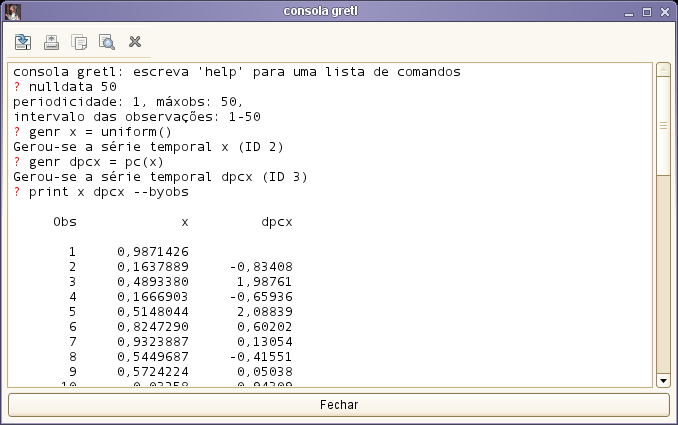
\includegraphics[scale=0.5]{figures/func_check}
  \caption{Output of function check}
  \label{fig:func_check}
\end{figure}

Now run your function. You may want to make sure it works properly by
running a few tests. For example, you may open the console and type

\begin{code}
genr x = uniform()
genr dpcx = pc(x)
print x dpcx --byobs
\end{code}

You should see something similar to figure \ref{fig:func_check}. The
function seems to work ok.  Once your function is debugged, you
may proceed to the next stage.

\subsection{Create a package}

We first present the mechanism for creating a function package via
\app{gretl}'s graphical interface. This can also be done via the
command line, which offers some additional functionality for package
authors; an explanation is given later in this section.

Start the GUI program and take a look at the ``File, Function files'' menu.
This menu contains four items: ``On local machine'', ``On server'', ``Edit
package'', ``New package''.

Select ``New package''.  (This will produce an error message unless at
least one user-defined function is currently loaded in memory --- see
the previous point.)  In the first dialog you get to select:

\begin{itemize}
\item A public function to package.
\item Zero or more ``private'' helper functions.
\end{itemize}

Public functions are directly available to users; private functions are
part of the ``behind the scenes'' mechanism in a function package.

\begin{figure}[htbp]
  \centering
  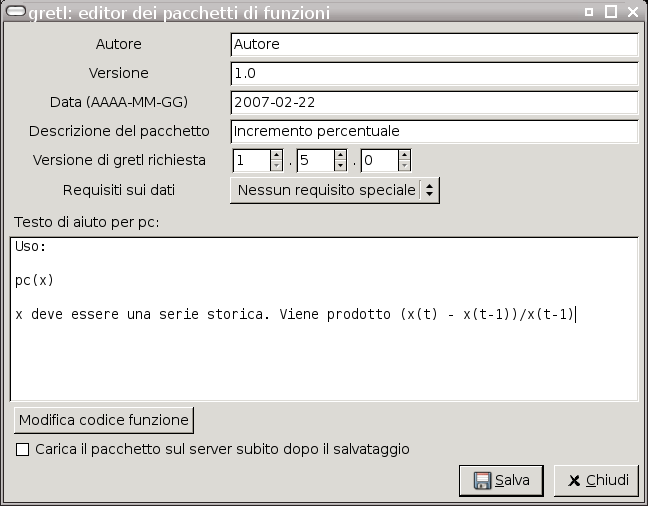
\includegraphics[scale=0.5]{figures/package_editor}
  \caption{The package editor window}
  \label{fig:package_editor}
\end{figure}

On clicking ``OK'' a second dialog should appear (see
Figure~\ref{fig:package_editor}), where you get to enter the package
information (author, version, date, and a short description).  You can
also enter help text for the public interface.  You have a further
chance to edit the code of the function(s) to be packaged, by clicking
on ``Edit function code''.  (If the package contains more than one
function, a drop-down selector will be shown.)  And you get to add a
sample script that exercises your package.  This will be helpful for
potential users, and also for testing.  A sample script is required if
you want to upload the package to the gretl server (for which a
check-box is supplied).

You won't need it right now, but the button labeled ``Save as script''
allows you to ``reverse engineer'' a function package, writing out a
script that contains all the relevant function definitions.

Clicking ``Save'' in this dialog leads you to a File Save dialog.  All
being well, this should be pointing towards a directory named
\texttt{functions}, either under the \app{gretl} system directory (if
you have write permission on that) or the \app{gretl} user directory.
This is the recommended place to save function package files, since
that is where the program will look in the special routine for opening
such files (see below).

Needless to say, the menu command ``File, Function files, Edit package''
allows you to make changes to a local function package.

\vspace{6pt}

A word on the file you just saved.  By default, it will have a
\texttt{.gfn} extension.  This is a ``function package'' file: unlike
an ordinary \app{gretl} script file, it is an XML file containing both
the function code and the extra information entered in the packager.
Hackers might wish to write such a file from scratch rather than using
the GUI packager, but most people are likely to find it awkward.  Note
that XML-special characters in the function code have to be escaped,
e.g.\ \texttt{\&} must be represented as \texttt{\&amp;}.  Also, some
elements of the function syntax differ from the standard script
representation: the parameters and return values (if any) are
represented in XML.  Basically, the function is pre-parsed, and ready
for fast loading using \textsf{libxml}.

\vspace{6pt}

\subsection{Load a package}

Why package functions in this way?  To see what's on offer so far, try
the next phase of the walk-through.

Close gretl, then re-open it.  Now go to ``File, Function files, On
local machine''. If the previous stage above has gone OK, you should
see the file you packaged and saved, with its short description.  If
you click on ``Info'' you get a window with all the information gretl
has gleaned from the function package.  If you click on the ``View
code'' icon in the toolbar of this new window, you get a script view
window showing the actual function code. Now, back to the ``Function
packages'' window, if you click on the package's name, the relevant
functions are loaded into \app{gretl}'s workspace, ready to be called
by clicking on the ``Call'' button.

After loading the function(s) from the package, open the GUI console.
Try typing \texttt{help foo}, replacing \texttt{foo} with the name of
the public interface from the loaded function package: if any help text
was provided for the function, it should be presented.

In a similar way, you can browse and load the function packages
available on the \app{gretl} server, by selecting ``File, Function
files, On server''.

Once your package is installed on your local machine, you can use the
function it contains via the graphical interface as described above,
or by using the CLI, namely in a script or through the console. In the
latter case, you load the function via the \texttt{include} command,
specifying the package file as the argument, complete with the
\texttt{.gfn} extension.

\begin{figure}[htbp]
  \centering
  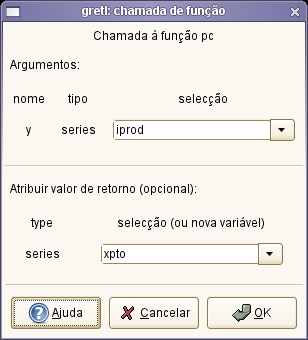
\includegraphics[scale=0.5]{figures/function_call}
  \caption{Using your package}
  \label{fig:function_call}
\end{figure}

To continue with our example, load the file \texttt{np.gdt} (supplied
with \app{gretl} among the sample datasets). Suppose you want to
compute the rate of change for the variable \texttt{iprod} via your
new function and store the result in a series named \texttt{foo}.

Go to ``File, Function files, On local machine''.  You will be shown a
list of the installed packages, including the one you have just
created. If you select it and click on ``Execute'' (or double-click on
the name of the function package), a window similar to the one shown
in figure \ref{fig:function_call} will appear.  Notice that the
description string ``Series to process'', supplied with the function
definition, appears to the left of the top series chooser.

Click ``Ok'' and the series \texttt{foo} will be generated (see figure
\ref{fig:iprod_pc}).  You may have to go to ``Data, Refresh data'' in
order to have your new variable show up in the main window variable
list (or just press the ``r'' key).

\begin{figure}[htbp]
  \centering
  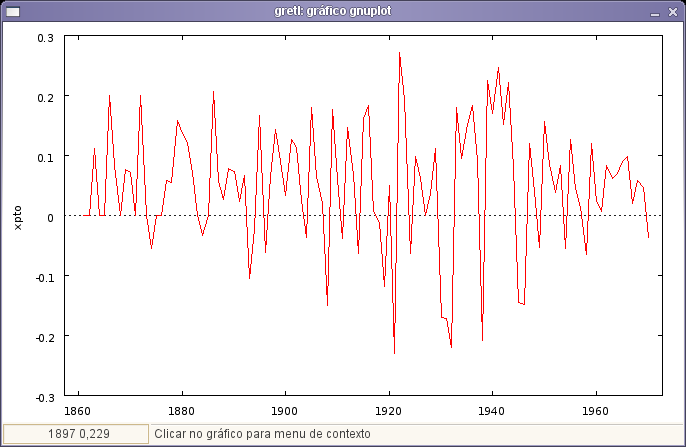
\includegraphics[scale=0.5]{figures/iprod_pc}
  \caption{Percent change in industrial production}
  \label{fig:iprod_pc}
\end{figure}

Alternatively, the same could have been accomplished by the script
\begin{code}
include pc.gfn
open np
foo = pc(iprod)
\end{code}

\subsection{Creating a package via the command line}

The mechanism described above, for creating function packages using
the GUI, is likely to be convenient for small to medium-sized packages
but may be too cumbersome for ambitious packages that include a large
hierarchy of private functions. To facilitate the building of such
packages \app{gretl} offers the \texttt{makepkg} command.

To use \texttt{makepkg} you create three files: a driver script that
loads all the functions you want to package and invokes
\texttt{makepkg}; a small, plain-text specification file that contains
the required package details (author, version, etc.); and (in the
simplest case) a plain text help file.  You run the driver script and
\app{gretl} writes the package (\texttt{.gfn}) file.

We first illustrate with a simple notional package. We have a gretl
script file named \texttt{foo.inp} that contains a function,
\texttt{foo}, that we want to package. Our driver script would then
look like this
%
\begin{code}
include foo.inp
makepkg foo.gfn
\end{code}
%
Note that the \texttt{makepkg} command takes one argument, the name of
the package file to be created. The package \emph{specification file}
should have the same basename but the extension \texttt{.spec}. In
this case \app{gretl} will therefore look for \texttt{foo.spec}. It
should look something like this:
%
\begin{code}
# foo.spec
author = A. U. Thor
version = 1.0
date = 2011-02-01
description = Does something with time series
public = foo 
help = foohelp.txt
sample-script = example.inp
min-version = 1.9.3
data-requirement = needs-time-series-data
\end{code}

As you can see, the format of each line in this file is \texttt{key =
  value}, with two qualifications: blank lines are permitted (and
ignored, as are comment lines that start with \verb|#|). 

All the fields included in the above example are required, with the
exception of \texttt{data-requirement}, though the order in which they
appear is immaterial. Here's a run-down of the basic fields:

\begin{itemize}
\item \texttt{author}: the name(s) of the author(s). Accented or other
  non-ASCII characters should be given as UTF-8.
\item \texttt{version}: the version number of the package, which should
  be limited to two integers separated by a period.
\item \texttt{date}: the release date of the current verson of the
  package, in ISO 8601 format: YYYY-MM-DD.
\item \texttt{description}: a brief description of the functionality
  offered by the package. This will be displayed in the GUI function
  packages window so it should be just one short line.
\item \texttt{public}: the listing of public functions.
\item \texttt{help}: the name of a plain text (UTF-8) file containing
  help; all packages must provide help.
\item \texttt{sample-script}: the name of a sample script that
 illustrates use of the package; all packages must supply a
 sample script.
\item \texttt{min-version}: the minimum version of gretl required
 for the package to work correctly. If you're unsure about this,
 the conservative thing is to give the current \app{gretl} version.
\end{itemize}

The \texttt{public} field indicates which function or functions are to
be made directly available to users (as opposed to private ``helper''
functions).  In the example above there is just one public
function. Note that any functions in memory when \texttt{makepkg} is
invoked, other than those designated as public, are assumed to be
private functions that should also be included in the package. That
is, the list of private functions (if any) is implicit.

The \texttt{data-requirement} field should be specified if the package
requires time-series or panel data, or alternatively if no dataset is
required.  If the \texttt{data-requirement} field is omitted, the
assumption is that the package needs a dataset in place, but it
doesn't matter what kind; if the packaged functions do not use any
series or lists this requirement can be explicitly relaxed.  Valid
values for this field are:

\begin{center}
\begin{tabular}{ll}
\texttt{needs-time-series-data} & (any time-series data OK) \\ 
\texttt{needs-qm-data} & (must be quarterly or monthly) \\ 
\texttt{needs-panel-data} & (must be a panel) \\
\texttt{no-data-ok} & (no dataset is needed) \\
\end{tabular}
\end{center}

For a more complex example, let's look at the \app{gig}
(GARCH-in-gretl) package.  The driver script for building \app{gig}
looks something like this:
%
\begin{code}
set echo off
set messages off
include gig_mle.inp
include gig_setup.inp
include gig_estimate.inp
include gig_printout.inp
include gig_plot.inp
makepkg gig.gfn
\end{code}

In this case the functions to be packaged (of which there are many)
are distributed across several script files, each of which is the
target of an \texttt{include} command.  The \texttt{set} commands at
the top are included to cut down on the verbosity of the output.

The content of \texttt{gig.spec} is as follows:
%
\begin{code}
author = Riccardo "Jack" Lucchetti and Stefano Balietti
version = 2.0
date = 2010-12-21
description = An assortment of univariate GARCH models
public = GUI_gig \
    gig_setup gig_set_dist gig_set_pq gig_set_vQR \
    gig_print gig_estimate \
    gig_plot gig_dplot \
    gig_bundle_print GUI_gig_plot

gui-main = GUI_gig
bundle-print = gig_bundle_print
bundle-plot = GUI_gig_plot
help = gig.pdf
sample-script = examples/example1.inp
min-version = 1.9.3
data-requirement = needs-time-series-data
\end{code}

Note that backslash continuation can be used for the elements of the
\texttt{public} function listing.

In addition to the fields shown in the simple example above,
\texttt{gig.spec} includes three optional fields: \texttt{gui-main},
\texttt{bundle-print} and \texttt{bundle-plot}. These keywords are
used to designate certain functions as playing a special role in the
\app{gretl} graphical interface. A function picked out in this way
must be in the \texttt{public} list and must satisfy certain
further requirements.  
%
\begin{itemize}
\item \texttt{gui-main}: this specifies a function as the one which
  will be presented automatically to GUI users (instead of users'
  being faced with a choice of interfaces). This makes sense only for
  packages that have multiple public functions. In addition, the
  \texttt{gui-main} function must return a \texttt{bundle} (see
  section~\ref{sec:Bundles}).
\item \texttt{bundle-print}: this picks out a function that should be
  used to print the contents of a bundle returned by the
  \texttt{gui-main} function. It must take a pointer-to-bundle as its
  first argument. The second argument, if present, should be an
  \texttt{int} switch, with two or more valid values, that controls the
  printing in some way. Any further arguments must have default values
  specified so that they can be omitted.
\item \texttt{bundle-plot}: selects a function for the role of
  producing a plot or graph based on the contents of a returned
  bundle. The requirements on this function are as for 
  \texttt{bundle-print}.
\end{itemize}

The ``GUI special'' tags support a user-friendly mode of operation.
On a successful call to \texttt{gui-main}, \app{gretl} opens a 
window displaying the contents of the returned bundle (formatted
via \texttt{bundle-print}). Menus in this window give the user the
option of saving the entire bundle (in which case it's represented
as an icon in the ``icon view'' window) or of extracting specific
elements from the bundle (series or matrices, for example). 

If the package has a \texttt{bundle-plot} function, the bundle window
also has a \textsf{Graph} menu. In \app{gig}, for example, the
\texttt{bundle-plot} function has this signature:
%
\begin{code}
function void GUI_gig_plot(bundle *model, int ptype[0:1:0] \
                           "Plot type" {"Time series", "Density"})
\end{code}

The \texttt{ptype} switch is used to choose between a time-series plot
of the residual and its conditional variance, and a kernel density
plot of the innovation against the theoretical distribution it is
supposed to follow. The use of the value-labels \texttt{Time series}
and \texttt{Density} means that the \textsf{Graph} menu will display
these two choices.

One other feature of the \app{gig} spec file is noteworthy: the
\texttt{help} field specifies \texttt{gig.pdf}, documentation in PDF
format. Unlike plain-text help, this cannot be rolled into the
\texttt{gfn} (XML) file produced by the \texttt{makepkg} command;
rather, both \texttt{gig.gfn} and \texttt{gig.pdf} are packaged into a
zip archive for distribution. This represents a form of package
which is new in \app{gretl} 1.9.4. More details will be made
available before long. 

\section{Memo: updating old-style functions}
\label{sec:old-func}

As mentioned at the start of this chapter, different rules were in
force for defining functions prior to \app{gretl} 1.8.4. While the old
syntax is still supported to date, this may not always be the
case. But it is straightforward to convert a function to the new
style. The only thing that must be changed for compatibility with the
new syntax is the declaration of the function's return
type. Previously this was placed inline in the \texttt{return}
statement, whereas now it is placed right after the \texttt{function}
keyword. For example:
%
\begin{code}
# old style
function triple (series x)
  y = 3*x
  return series y # note the "series" here
end function

# new style
function series triple (series x)
  y = 3*x
  return y
end function
\end{code}

Note also that the role of the \texttt{return} statement has changed
(and its use has become more flexible):

\begin{itemize}
\item The \texttt{return} statement now causes the function to return
  directly, and you can have more than one such statement, wrapped in
  conditionals. Before there could only be one \texttt{return}
  statement, and its role was just to specify the type available for
  assignment by the caller.
\item The final element in the \texttt{return} statement can now be an
  expression that evaluates to a value of the advertised return type;
  before, it had to be the name of a pre-defined variable.
\end{itemize}


%%% Local Variables: 
%%% mode: latex
%%% TeX-master: "gretl-guide"
%%% End: 


\chapter{Liste e stringhe definite dall'utente}
\label{chap-persist}

\section{Liste definite dall'utente}
\label{named-lists}

Molti comandi di \app{gretl} richiedono come argomenti una o pi� liste di
variabili. Per semplificare la loro gestione negli script di comandi, in
particolare nelle funzioni definite dall'utente, \app{gretl} offre la
possibilit� di creare \textit{liste definite dall'utente}.  

\subsection{Creazione e modifica di una lista}

Per creare una lista occorre usare il comando \texttt{list}, seguito dal nome
della lista, un segno di uguale, e, in alternativa, \texttt{null} (per creare
una lista vuota) o il nome di una o pi� variabili da inserire nella lista. Ad
esempio:
%
\begin{code}
list xlist = 1 2 3 4
list reglist = income price 
list empty_list = null
\end{code}

� disponibile una forma speciale: se si usa la parola chiave \texttt{dataset}
al posto di una lista vera e propria di variabili, verr� costruita una lista che
contiene tutte le serie di dati del dataset in uso (tranne che per la costante
predefinita \texttt{const}).

Il nome della lista deve iniziare con una lettera e deve essere composto
interamente da lettere, numeri o il carattere trattino basso (non da spazi). La
lunghezza massima del nome � di 15 caratteri. Quando si aggiungono variabili a
una lista � possibile riferirsi a essa per nome o per numero identificativo.

Una volta creata, una lista viene ``ricordata'' per l'intera durata della
sessione di \app{gretl} e pu� essere usata nel contesto di qualsiasi comando
\app{gretl} che accetta liste di variabili. Un semplice esempio � la
specificazione di una lista di regressori:
%
\begin{code}
list xlist = x1 x2 x3 x4
ols y 0 xlist
\end{code}

Le liste possono essere modificate in due modi. Per \textit{ridefinire} una
lista si usa la stessa sintassi usata per crearla. Ad esempio
%
\begin{code}
list xlist = 1 2 3
list xlist = 4 5 6
\end{code}

Dopo il secondo comando, \texttt{xlist} contiene solo le variabili 4,
5 e 6.

Per \textit{accodare} o \textit{premettere} variabili a una lista esistente,
� possibile usare il nome di una lista all'interno del comando di definizione
della lista stessa. Ad esempio, � possibile scrivere
%
\begin{code}
list xlist = xlist 5 6 7
list xlist = 9 10 xlist 11 12
\end{code}
%
Un altro modo per accodare un termine a una lista consiste nell'usare l'operatore \texttt{+=},
come in
%
\begin{code}
list xlist += cpi
\end{code}
%
Per eliminare una variabile da una lista, basta usare l'operatore \texttt{-=}:
%
\begin{code}
list xlist -= cpi
\end{code}
%

\subsection{Interrogazione delle liste}

� possibile determinare se una variabile sconosciuta rappresenta una lista
usando la funzione \texttt{islist()}.
%
\begin{code}
series xl1 = log(x1)
series xl2 = log(x2)
list xlogs = xl1 xl2
genr is1 = islist(xlogs)
genr is2 = islist(xl1)
\end{code}

Il primo comando \texttt{genr} assegner� il valore 1 a \texttt{is1} visto che
\texttt{xlogs} in effetti � una lista. Il secondo comando genr assegner� il
valore 0 a \texttt{is2}, visto che \texttt{xl1} � una serie di dati, non una
lista.

� anche possibile determinare il numero di elementi che compongono una lista
usando la funzione \texttt{nelem()}.
%
\begin{code}
list xlist = 1 2 3
genr nl = nelem(xlist)
\end{code}

Lo scalare \texttt{nl} avr� un valore di 3, visto che
\texttt{xlist} contiene 3 membri.

� possibile mostrare i membri di una lista come illustrato in questa sessione
interattiva:
%
\begin{code}
? list xlist = x1 x2 x3
 # list xlist = x1 x2 x3
Added list 'xlist'
? list xlist print
 # list xlist = x1 x2 x3
\end{code}
%
Si noti che \texttt{print xlist} produrr� un effetto diverso, ossia mostrer� i
valori di tutte le variabili contenute in \texttt{xlist} (come ci si pu�
aspettare).

\subsection{Liste di variabili trasformate}

Data una lista di variabili, � possibile generare liste che contengono
trasformazioni di queste variabili usando una forma speciale dei comandi
\texttt{logs}, \texttt{lags}, \texttt{diff}, \texttt{ldiff},
\texttt{sdiff} o \texttt{square}. In pratica basta far seguire questi comandi
dal nome della lista tra parentesi. Ad esempio:
%
\begin{code}
list xlist = x1 x2 x3
list lxlist = logs(xlist)
list difflist = diff(xlist)
\end{code}

Quando si genera una lista di \textit{ritardi} in questo modo, � possibile
specificare il massimo ordine di ritardi, inserendolo per primo tra parentesi e
separandolo dal nome della lista con una virgola. Ad esempio
%
\begin{code}
list xlist = x1 x2 x3
list laglist = lags(2, xlist)
\end{code}
%
oppure
%
\begin{code}
scalar order = 4
list laglist = lags(order, xlist)
\end{code}

Questi comandi riempiranno \texttt{laglist} col numero specificato di ritardi
delle variabili presenti in \texttt{xlist}. Come avviene per il normale comando
\texttt{lags} � possibile omettere l'ordine, che sar� cos� determinato
automaticamente a seconda della frequenza dei dati. Un altro modo speciale di
utilizzare questi comandi consiste nell'indicare tra parentesi il nome di una
singola variabile al posto di quello di una lista, come in
%
\begin{code}
series lx = log(x)
list laglist = lags(4, lx)
\end{code}

Si noti che la sintassi normale per questi comandi, ad esempio \texttt{logs},
� semplicemente
%
\begin{code}
logs x1 x2 x3
\end{code}
%
Se \texttt{xlist} � una lista, � anche possibile scrivere
%
\begin{code}
logs xlist
\end{code}
%
ma questo comando non salver� i logaritmi in una lista; per avere questo
risultato occorre usare la sintassi
%
\begin{code}
list loglist = logs(xlist)
\end{code}


\subsection{Controllo dei valori mancanti}

\app{Gretl} offre varie funzioni per riconoscere e gestire i valori mancanti (si
veda la \GCR{} per i dettagli). In questa sede � utile ricordare che la funzione
\texttt{ok()} pu� essere usata con un argomento lista. Ad esempio:
%
\begin{code}
list xlist = x1 x2 x3
series xok = ok(xlist)
\end{code}
%
Dopo questi comandi, la serie \texttt{xok} avr� valore 1 per le osservazioni in
cui nessuna variabile tra \texttt{x1}, \texttt{x2}, e
\texttt{x3} ha un valore mancante, e valore 0 per le osservazioni che non
soddisfano questa condizione.


\section{Stringhe definite dall'utente}
\label{named-strings}

In alcuni casi pu� essere utile salvare una stringa (ossia una sequenza di
caratteri) sotto forma di variabile che possa essere riutilizzata.
\app{Gretl} offre questa funzionalit� a partire dalla versione 1.6.0, ma alcune
delle caratteristiche mostrate di seguito sono disponibili solo a partire dalla
versione 1.7.2.

Per \textit{definire} una variabile stringa � possibile usare uno dei comandi
seguenti: \texttt{string} o \texttt{sprintf}.  Il comando \texttt{string}
� il pi� semplice: basta scrivere, ad esempio
%
\begin{code}
string s1 = "Qualcosa da ricordare"
string s2 = getenv("HOME")
string s3 = @pippo + 10
\end{code}
%
Il primo campo dopo \texttt{string} � il nome della variabile che verr� creata,
quindi segue il segno di uguale, infine una specificazione della stringa da salvare.
Quest'ultima pu� essere la parola chiave \texttt{null}, per produrre una stringa
nulla, oppure pu� assumere una delle forme seguenti:

\begin{itemize}
\item una stringa letterale (racchiusa tra virgolette doppie)
\item il nome di una variabile stringa esistente, prefissata con \verb|@|
\item una funzione che produce una stringa (si veda oltre)
\item una delle forme viste finora, seguita da \texttt{+} e un valore intero che
  indica una posizione
\item una delle forme viste finora, seguita da uno spazio, seguito da un altro
  campo simile
\end{itemize}

Il ruolo del valore intero di posizione permette di usare una sotto-stringa
dell'elemento precedente, a partire dal carattere specificato. Se il valore
del parametro di posizione � maggiore della lunghezza della stringa in
questione, viene prodotto un messaggio di errore.

Nel caso in cui vengano usate due specificazioni separate da spazio, la stringa
risultante � la concatenazione dei due elementi.

Il comando \texttt{sprintf} � pi� flessibile. Funziona esattamente come
\texttt{printf} di \app{gretl}, tranne per il fatto che la stringa ``di formato'' deve
essere preceduta dal nome di una variabile stringa. Ad esempio,
%
\begin{code}
scalar x = 8
sprintf pippo "var%d", x
\end{code}

Per \textit{recuperare il valore} di una variabile stringa, basta usare il nome
della variabile preceduto dal carattere ``at'', \verb|@|.

In molti contesti la notazione \verb|@| � trattata come una ``macro'', ossia in
un comando \app{gretl} una sequenza di caratteri che segue il simbolo \verb|@|
viene trattata come il nome di una variabile stringa e il valore della variabile
viene sostituito sulla riga di comando, come avviene in questo esempio di
sessione interattiva:
%
\begin{code}
? scalar x = 8
 scalar x = 8
Generato lo scalare x (ID 2) = 8
? sprintf pippo "var%d", x
Salvata la stringa 'pippo'
? print "@foo"
var8
\end{code}
%
Si noti l'effetto delle virgolette doppie nella riga
\verb|print "@foo"|.  La riga
%
\begin{code}
? print @foo
\end{code}
%
\textit{non} stamperebbe un ``\texttt{var8}'' letteralmente, come visto sopra.
La riga verrebbe processata e letta come
%
\begin{code}
print var8
\end{code}
%
Quindi stamperebbe i valori della variabile \texttt{var8}, se esiste, oppure un
messaggio di errore.

In alcuni contesti specifici, comunque, � naturale trattare le variabili
\verb|@| come variabili a tutti gli effetti, e \app{gretl} si comporta proprio
cos�. Questo avviene quando le variabili appaiono:
\begin{itemize}
\item come argomenti dei comandi \texttt{printf} e
  \texttt{sprintf}.
\item nella parte destra di un'istruzione \texttt{string}.
\item come argomenti della funzione \texttt{isstring} (si veda sotto).
\end{itemize}

Ecco un esempio di uso delle stringhe come argomenti di
\texttt{printf}:
%
\begin{code}
? string vstr = "varianza"
Salvata stringa 'vstr'
? printf "vstr: %12s\n", @vstr
vstr:     varianza
\end{code}
%
Si noti che \verb|@vstr| non dovrebbe essere messa tra virgolette in questo
contesto. Allo stesso modo con
\begin{code}
? string copy = @vstr
\end{code}

\subsection{Stringhe predefinite}

Oltre alle stringhe definite dall'utente, \app{gretl} contiene alcune variabili
stringa predefinite che possono essere utili per chi scrive funzioni che
includono comandi shell. Le stringhe predefinite sono mostrate nella
Tabella~\ref{tab-strings}.

\begin{table}[htbp]
\centering
\begin{tabular}{ll}
  \verb|@gretldir| & La directory di installazione di \app{gretl} \\
  \verb|@workdir| & La directory di lavoro di \app{gretl} per l'utente \\
  \verb|@gnuplot| & Percorso, o nome, dell'eseguibile \app{gnuplot} \\
  \verb|@tramo| & Percorso, o nome, dell'eseguibile \app{tramo} \\
  \verb|@x12a| & Percorso, o nome, dell'eseguibile \app{x-12-arima} \\
  \verb|@tramodir| & Directory dei dati di \app{tramo} \\
  \verb|@x12adir| & Directory dei dati di \app{x-12-arima} \\
\end{tabular}
\caption{Variabili stringa predefinite}
\label{tab-strings}
\end{table}

\subsection{Lettura delle stringhe dall'ambiente}

In aggiunta, � possibile importare all'interno delle stringhe di \app{gretl}
dei valori che sono definiti nell'ambiente esterno. Per fare questo occorre
usare la funzione \texttt{getenv}, che richiede come argomento il nome di una
variabile di ambiente. Ad esempio:
%
\begin{code}
? string user = getenv("USER")
Salvata la stringa 'user'
? string home = getenv("HOME")
Salvata la stringa 'home'
? print "La home directory di @user � @home"
La home directory di cottrell � /home/cottrell
\end{code}
%
Per controllare se la variabile di ambiente richiamata da \texttt{getenv} �
non-vuota, si pu� usare la funzione \texttt{isstring}, come in questo esempio
%
\begin{code}
? string temp = getenv("TEMP")
Salvata la stringa vuota 'temp'
? scalar x = isstring(@temp)
Generato lo scalare x (ID 2) = 0
\end{code}
%
Si noti che \texttt{isstring} significa ``� una stringa che contiene
effettivamente qualcosa''.

Al momento la funzione \texttt{getenv} pu� essere usata solo nella parte destra
di un'istruzione \texttt{string}, come negli esempi visti sopra.

\subsection{Lettura delle stringhe usando la shell}

Se in \app{gretl} sono stati abilitati i comandi shell, � possibile catturare i
risultati dei comandi usando la sintassi

\texttt{string} \textsl{nome-stringa} = \texttt{\$(}\textsl{comando-shell}\texttt{)}

Ossia, si include il comando shell tra parentesi precedute dal carattere
dollaro.

\subsection{Lettura delle stringhe da file}

� possibile leggere il contenuto di un file e scriverlo all'interno di una
variabile stringa usando la sintassi

\texttt{string} \textsl{nome-stringa} = \texttt{readfile(}\textsl{nome-file}\texttt{)}

Il campo \textsl{nome-file} pu� includere variabili stringa. Ad esempio

\verb|string qnc = readfile(@x12adir/QNC.rts)|

\subsection{La funzione \texttt{strstr}}

Questa funzione viene usata nel modo seguente

\texttt{string} \textsl{nome-stringa} = 
\texttt{strstr(}\textsl{s1}\texttt{,} \textsl{s2}\texttt{)}

L'effetto � quello di cercare all'interno di \textsl{s1} la prima occorrenza di
\textsl{s2}.  Se non viene trovato alcun risultato, viene prodotta una stringa
vuota, altrimenti viene prodotta la porzione di \textsl{s1} che inizia per
\textsl{s2}. Ad esempio:
%
\begin{code}
? string hw = "hello world"
Saved string as 'hw'
? string w = strstr(@hw, "o")
Saved string as 'w'
? print "@w"
o world
\end{code}
%


%%% Local Variables: 
%%% mode: latex
%%% TeX-master: "gretl-guide"
%%% End: 


\chapter{Operazioni con le matrici}
\label{chap:matrices}

\section{Creazione di matrici}
\label{matrix-create}

� possibile creare una matrice usando uno dei metodi seguenti:

\begin{enumerate}
\item Specificando direttamente i valori scalari che compongono la matrice,
  in forma numerica, per riferimento a variabili scalari preesistenti, o usando
  valori calcolati;
\item fornendo una lista di serie di dati;
\item fornendo una \textit{lista personalizzata} di serie;
\item usando una formula simile a quelle usate con il comando
  \texttt{genr}, in cui una nuova matrice viene definita in termini di matrici
  e/o scalari esistenti, oppure attraverso funzioni speciali.
\end{enumerate}

Per specificare una matrice \textit{direttamente in termini di scalari}, la
sintassi � la seguente:

\begin{code}
matrix A = { 1, 2, 3 ; 4, 5, 6 }
\end{code}

La matrice viene definita per righe successive; gli elementi di ogni riga sono
separati da virgole e le righe sono separate da punti e virgola. L'intera
espressione va racchiusa tra parentesi graffe. Gli spazi tra le parentesi non
sono significativi. L'espressione vista sopra definisce una matrice $2\times 3$.
Ogni elemento deve essere un valore numerico, il nome di una variabile scalare
preesistente, o un'espressione che, valutata, produce uno scalare.
Per ottenere la matrice trasposta, basta aggiungere un apostrofo
(\texttt{'}) direttamente dopo la parentesi graffa che chiude l'espressione.

Per specificare una matrice \textit{in termini di serie di dati} la sintassi �
la seguente:
%
\begin{code}
matrix A = { x1, x2, x3 }
\end{code}
%
dove i nomi delle variabili sono separati da virgole. Oltre ai nomi di variabili
esistenti, � possibile usare espressioni che producono una serie una volta
valutate. Ad esempio, data una serie \texttt{x}, si pu� scrivere
%
\begin{code}
matrix A = { x, x^2 }
\end{code}
%

Ogni variabile rappresenta una colonna (e pu� esserci solo una variabile per
ogni colonna). Non � possibile usare il carattere di punto e virgola come
separatore di riga in questo caso: se si vuole che le serie siano disposte per
righe, occorre usare il simbolo di trasposizione.  L'intervallo dei valori dei
dati inclusi nella matrice dipende dall'impostazione corrente dell'intervallo
del campione.

Si noti che mentre le funzioni statistiche di gretl sono in grado di gestire
valori mancanti, ci� non vale per le funzioni che trattano le matrici:
\emph{quando si costruisce una matrice partendo da serie che contengono valori
mancanti, le osservazioni per cui almeno una delle serie contiene valori
mancanti sono saltate}.

Invece di fornire una lista esplicita di variabili, � possibile fornire il
\textit{nome di una lista personalizzata} (si veda il capitolo~\ref{chap-persist}),
come nell'esempio seguente:
%
\begin{code}
list xlist = x1 x2 x3
matrix A = { xlist }
\end{code}
%
Se si usa il nome di una lista, le serie che la costituiscono vengono usate per
comporre le colonne, come risulta naturale in un contesto econometrico; se si
vuole che vengano usate come righe, basta usare il simbolo di trasposizione.

Un caso speciale di costruzione di una matrice usando una lista di variabili
� il seguente:
%
\begin{code}
matrix A = { dataset }
\end{code}
%
In questo modo, si costruisce una matrice usando tutte le serie del dataset
corrente, salvo la costante (variabile 0). Quando si usa questa lista speciale,
essa deve essere il solo elemento nella definizione della matrice \texttt{\{...\}}.
� tuttavia possibile creare una matrice che includa la costante, oltre alle
altre variabili, usando la concatenazione per colonne (si veda oltre), come
in questo esempio:
%
\begin{code}
matrix A = {const}~{dataset}
\end{code}
%

� possibile creare nuove matrici, o sostituire matrici esistenti, usando varie
trasformazioni, come per gli scalari e le serie di dati. I prossimi paragrafi
spiegano nel dettaglio questi meccanismi.

La sintassi
%
\begin{code}
matrix A = {}
\end{code}
%
crea una matrice vuota, ossia una matrice con zero righe e zero colonne.
Si veda la sezione \ref{sec:emptymatrix} per una discussione di questo oggetto.

\tip{I nomi delle matrici devono soddisfare gli stessi requisiti dei nomi delle
variabili in gretl: il nome non pu� essere pi� lungo di 15 caratteri, deve
iniziare per una lettera e deve essere composto da lettere, numeri e il
carattere trattino basso.}

\section{Selezione di sotto-matrici}
\label{matrix-sub}

� possibile selezionare delle sotto-matrici a partire da una matrice usando la
sintassi:

\texttt{A[}\textsl{righe},\textsl{colonne}\texttt{]}

dove \textsl{righe} pu� avere una delle seguenti forme:

\begin{center}
\begin{tabular}{ll}
Vuoto & seleziona tutte le righe \\
Un valore intero & seleziona la riga identificata dal numero \\
Due interi separati dal carattere due punti & seleziona un intervallo di righe \\
Il nome di una matrice & seleziona le righe specificate dai valori della matrice \\
\end{tabular}
\end{center}

Rispetto alla seconda opzione, il valore intero pu� essere indicato
numericamente, attraverso il nome di una variabile scalare esistente, o
con un'espressione che, valutata, produce uno scalare.
Con l'ultima opzione, la matrice indicata nel campo \textsl{righe} deve
avere dimensioni $p\times 1$ o $1\times p$ e deve contenere valori interi
nell'intervallo da 1 a $n$, dove $n$ � il numero di righe da selezionare
dalla matrice principale.

L'uso del parametro \textsl{colonne} � simile, \textit{mutatis
  mutandis}.  Ecco alcuni esempi.
%
\begin{code}
matrix B = A[1,]
matrix B = A[2:3,3:5]
matrix B = A[2,2]
matrix idx = { 1, 2, 6 }
matrix B = A[idx,]
\end{code}
%
Il primo esempio seleziona la prima riga dalla matrice \texttt{A}; il secondo
seleziona una sotto-matrice $2\times 3$; il terzo seleziona uno scalare, mentre
il quarto seleziona le righe 1, 2 e 6 dalla matrice \texttt{A}.

In aggiunta, c'� una specificazione di indice predefinita, \texttt{diag},
seleziona la diagonale principale di una matrice quadrata, come in
\texttt{B[diag]}, dove \texttt{B} � quadrata.

� possibile usare la selezione di sotto-matrici sia a destra sia a sinistra in
una formula che genera una matrice. Ecco un esempio di uso della selezione nella
parte destra, per estrarre una sotto-matrice $2\times 2$ $B$ da una matrice
$3\times 3$ $A$:
%
\begin{code}
matrix A = { 1, 2, 3; 4, 5, 6; 7, 8, 9 }
matrix B = A[1:2,2:3]
\end{code}
%
Ed ecco un esempio di selezione sulla sinistra. La seconda riga nell'esempio
scrive una matrice identit� $2\times 2$ nell'angolo inferiore destro della matrice
$3\times 3$ $A$. La quarta riga rimpiazza la diagonale di $A$ con valori 1.
%
\begin{code}
matrix A = { 1, 2, 3; 4, 5, 6; 7, 8, 9 }
matrix A[2:3,2:3] = I(2)
matrix d = { 1, 1, 1 }
matrix A[diag] = d
\end{code}

\section{Operatori matriciali}
\label{matrix-op}

Per le matrici sono disponibili i seguenti operatori binari:

\begin{center}
\begin{tabular}{ll}
\texttt{+} & addizione \\
\texttt{-} & sottrazione \\
\texttt{*} & moltiplicazione matriciale \\
\texttt{'} & premoltiplicazione per la trasposta \\
\texttt{/} & ``divisione'' matriciale (si veda oltre) \\
\verb+~+ & concatenazione per colonne \\
\verb+|+ & concatenazione per righe \\
\texttt{**} & prodotto di Kronecker \\
\texttt{=} & test per l'uguaglianza 
\end{tabular}
\end{center}

Inoltre, i seguenti operatori (operatori ``punto'') funzionano elemento per
elemento:

\begin{center}
\begin{tabular}{cccccc}
\texttt{.*}  &  \texttt{./}  &  \verb+.^+  &
\texttt{.=}  &  \texttt{.>}  &  \texttt{.<} 
\end{tabular}
\end{center}

Ecco qualche spiegazione per i casi meno ovvi.

Per l'addizione e la sottrazione matriciale, in generale le due matrici
devono avere le stesse dimensioni, salvo il caso in cui uno dei termini
� una matrice $1\times 1$ o uno scalare. In questo caso, lo scalare viene
implicitamente trasformato in una matrice con le corrette dimensioni, i cui
elementi sono tutti pari al valore dello scalare. Ad esempio, se
$A$ � una matrice $m \times n$ e $k$ � uno scalare, i comandi
%
\begin{code}
matrix C = A + k
matrix D = A - k
\end{code}
%
producono entrambi delle matrici $m \times n$, con elementi $c_{ij} = 
+a_{ij} + k$ e $d_{ij} = a_{ij} - k$ rispettivamente.
 
Per ``moltiplicazione per la trasposta'' si intende, ad esempio, che
%
\begin{code}
matrix C = X'Y
\end{code}
%
ha come risultato il prodotto fra $X$-trasposta e $Y$.  In effetti, 
l'espressione \texttt{X'Y} ha lo stesso significato di \texttt{X'*Y}
(che pure � un comando valido).

La ``divisione'' tra matrici, $A/B$ � algebricamente equivalente a $B^{-1}A$
(pre-moltiplicazione per mezzo dell'inversa del ``divisore''). Quindi in linea
di principio le due espressioni seguenti sono equivalenti:
%
\begin{code}
matrix C = A / B
matrix C = inv(B) * A
\end{code}
%
dove \texttt{inv} � la funzione di inversione tra matrici (si veda oltre).
Per� la prima forma pu� essere pi� accurata della seconda, perch� la soluzione �
ottenuta tramite la scomposizione LU, senza calcolare esplicitamente la matrice
inversa.

Nella \textit{moltiplicazione per elementi}, scrivendo
%
\begin{code}
matrix C = A .* B
\end{code}
% 
il risultato dipende dalle dimensioni di $A$ e $B$. Se $A$ � una matrice
$m \times n$ e $B$ � una matrice $p \times q$.  
%
\begin{itemize}
\item Se $m=p$ e $n=q$, $C$ sar� una matrice $m\times n$ con $c_{ij} = a_{ij}
  \times b_{ij}$. Questo tipo di prodotto � tecnicamente noto come
  \emph{prodotto di Hadamard}.
\item Se $m=1$ e $n=q$, oppure $n=1$ e $m=p$, $C$ sar� una matrice
  $p\times q$ con $c_{ij} = a_k \times b_{ij}$, dove $k=j$ se $m=1$,
  altrimenti $k=i$.
\item Se $p=1$ e $n=q$, oppure $q=1$ e $m=p$, $C$ sar� una matrice
  $m\times n$ con $c_{ij} = a_{ij} \times b_k$, dove $k=j$ se $p=1$,
  altrimenti $k=i$.
\item Se non � soddisfatta alcuna delle condizioni precedenti, il prodotto non �
  definito e viene segnalato un errore.
\end{itemize}
Ad esempio, se $A$ � un vettore riga con lo stesso numero di colonne di
$B$, le colonne di $C$ sono le colonne di $B$ moltiplicate per i corrispondenti
elementi di $A$. Si noti che questa convenzione rende superfluo, nella maggior
parte dei casi, usare matrici diagonali per eseguire trasformazioni usando la
moltiplicazione ordinaria tra matrici: se $Y = XV$, dove $V$ � diagonale, �
molto pi� comodo dal punto di vista computazionale ottenere $Y$ usando
l'istruzione
%
\begin{code}
matrix Y = X .* v
\end{code}
%
dove \texttt{v} � un vettore riga che contiene la diagonale di $V$.
 
La divisione per elementi e l'elevamento a potenza per elementi funzionano in
modo analogo alla moltiplicazione per elementi, sostituendo $\times$ con $\div$,
o con l'operazione di elevamento a potenza, nella spiegazione precedente.

Nella \textit{concatenazione per colonne} di una matrice $A$ $m\times n$ e di una
matrice $B$ $m\times p$, il risultato � una matrice $m\times (n+p)$. Ossia:
%
\begin{code}
matrix C = A ~ k
\end{code}
% 
produce $C = \left[ \begin{array}{cc} A & B \end{array} \right]$.

La \textit{concatenazione per righe} di una matrice $A$ $m\times n$ e di una matrice $B$
$p\times n$ produce una matrice $(m+p) \times n$.
%
\begin{code}
C = A | B
\end{code}
% 
produce $C = \left[ \begin{array}{cc} A \\ B \end{array} \right]$.

\section{Operatori matrice-scalare}
\label{matrix-scalar-op}

Per una matrice $A$ e uno scalare $k$, sono disponibili gli operatori mostrati nella
Tabella~\ref{tab:matrix-scalar-ops} (addizione e sottrazione sono state
presentate nella sezione~\ref{matrix-op} ma sono incluse nella tabella per
completezza). Inoltre, per una matrice quadrata $A$ e un intero $k \geq 0$,
\verb|B = A^k| produce una matrice $B$ che � $A$ elevata alla potenza $k$.
Si noti che l'operatore \texttt{**} non pu� essere usato al posto di \verb|^|
a questo scopo, perch� in un contesto matriciale esso � riservato per il prodotto
di Kronecker.

\begin{table}[htbp]
\centering
\begin{tabular}{ll}
\textit{Espressione} & \textit{Risultato} \\[4pt]
\texttt{matrix B = A * k} & $b_{ij} = k a_{ij}$ \\
\texttt{matrix B = A / k} & $b_{ij} = a_{ij} / k$ \\
\texttt{matrix B = k / A} & $b_{ij} = k / a_{ij}$ \\
\texttt{matrix B = A + k} & $b_{ij} = a_{ij} + k$ \\
\texttt{matrix B = A - k} & $b_{ij} = a_{ij} - k$ \\
\texttt{matrix B = k - A} & $b_{ij} = k - a_{ij}$ \\
\texttt{matrix B = A \% k} & $b_{ij} = a_{ij} \mbox{ modulo } k$ \\
\end{tabular}
\caption{Operatori matrice--scalare}
\label{tab:matrix-scalar-ops}
\end{table}

\section{Funzioni matriciali}
\label{matrix-func}

\newlength{\cwid}
\setlength{\cwid}{0.1\textwidth}

\begin{table}[htbp]
\centering
\textbf{Creazione e I/O}
\hrulefill

\begin{tabular}{p{\cwid}p{\cwid}p{\cwid}p{\cwid}p{\cwid}p{\cwid}}
\texttt{I}         &
\texttt{mnormal}   &
\texttt{mread}     &
\texttt{mwrite}    &
\texttt{muniform}  &
\texttt{ones}      \\
\texttt{seq}       &
\texttt{zeros}     
\end{tabular}      

\textbf{Forma/dimensione}
\hrulefill

\begin{tabular}{p{\cwid}p{\cwid}p{\cwid}p{\cwid}p{\cwid}p{\cwid}}
\texttt{cols}      &
\texttt{diag}      &
\texttt{dsort}     &
\texttt{mlag}      &
\texttt{mshape}    &
\texttt{rows}      \\
\texttt{sort}      &
\texttt{transp}    &
\texttt{unvech}    &
\texttt{vec}       &
\texttt{vech}      
\end{tabular}      

\textbf{Elemento per elemento}
\hrulefill

\begin{tabular}{p{\cwid}p{\cwid}p{\cwid}p{\cwid}p{\cwid}p{\cwid}}
\texttt{abs}       &
\texttt{atan}      &
\texttt{cnorm}     &
\texttt{cos}       &
\texttt{dnorm}     &
\texttt{exp}       \\
\texttt{gamma}     &
\texttt{int}       &
\texttt{lngamma}   &
\texttt{log}       &
\texttt{qnorm}     &
\texttt{sin}       \\
\texttt{sqrt}      &
\texttt{tan}       
\end{tabular}      

\textbf{Algebra matriciale}
\hrulefill

\begin{tabular}{p{\cwid}p{\cwid}p{\cwid}p{\cwid}p{\cwid}p{\cwid}}
\texttt{cholesky}  &
\texttt{det}       &
\texttt{eigengen}  &
\texttt{eigensym}  &
\texttt{fft}       &
\texttt{ffti}      \\
\texttt{infnorm}   &
\texttt{inv}       &
\texttt{invpd}     &
\texttt{ginv}      &
\texttt{ldet}      &
\texttt{mexp}      \\
\texttt{nullspace} &
\texttt{onenorm}   &
\texttt{qform}     &
\texttt{qrdecomp}  &
\texttt{rank}      &
\texttt{rcond}     \\
\texttt{svd}       &
\texttt{tr}        &
\texttt{cmult}     &
\texttt{cdiv}
\end{tabular}      

\textbf{Statistica}
\hrulefill

\begin{tabular}{p{\cwid}p{\cwid}p{\cwid}p{\cwid}p{\cwid}p{\cwid}}
\texttt{cdemean}   &
\texttt{imaxc}     &
\texttt{imaxr}     &
\texttt{iminc}     &
\texttt{iminr}     &
\texttt{mcorr}     \\
\texttt{mcov}      &
\texttt{maxc}      &   
\texttt{maxr}      &
\texttt{meanc}     &
\texttt{meanr}     &
\texttt{minc}      \\   
\texttt{minr}      &
\texttt{mols}      &
\texttt{mxtab}     &
\texttt{princomp}  &
\texttt{sumc}      &
\texttt{sumr}      \\
\texttt{sd}        &
\texttt{values}
\end{tabular}

\caption{Funzioni matriciali suddivise per categoria}
\label{tab:matrix_funcs_cat}
\end{table}

La tabella \ref{tab:matrix_funcs_cat} elenca le funzioni matriciali fornite da
\app{gretl} (una versione ordinata in ordine alfabetico della tabella � fornita
alla fine di questo capitolo, si veda la Tabella~\ref{tab:matrix_funcs}).
Per \textit{la trasformazione elemento per elemento} delle matrici sono
disponibili le seguenti funzioni: \texttt{log}, \texttt{exp},
\texttt{sin}, \texttt{cos}, \texttt{tan}, \texttt{atan}, \texttt{int},
\texttt{abs}, \texttt{sqrt}, \texttt{dnorm}, \texttt{cnorm},
\texttt{qnorm}, \texttt{gamma} e \texttt{lngamma}. Queste funzioni operano in
modo analogo a quando sono usate nel contesto del comando \texttt{genr}.  Ad
esempio, se una matrice \texttt{A} � gi� stata definita,
%
\begin{code}
matrix B = sqrt(A)
\end{code}
%
genera una matrice tale che $b_{ij} = \sqrt{a_{ij}}$.  Tutte queste
funzioni richiedono una sola matrice come argomento, o un'espressione
che si risolve in una singola matrice.

Si noti che per calcolare la ``radice quadrata di una matrice'' occorre la
funzione \texttt{cholesky} (si veda oltre); inoltre, la funzione
\texttt{exp} calcola l'esponenziale elemento per elemento, quindi \emph{non}
produce l'esponenziale della matrice, a meno che la matrice non sia diagonale;
per calcolare l'esponenziale della matrice, si usi \texttt{mexp}.

Le funzioni \texttt{sort}, \texttt{dsort} e \texttt{values}, utilizzabili
con le serie di dati, possono essere usate anche con le matrici.  In questo
caso, l'argomento di queste funzioni deve essere un vettore ($p \times 1$ o
$1\times p$). Per \texttt{sort} e \texttt{dsort}, il valore restituito � un
vettore che contiene gli elementi del vettore originale riordinati in ordine di
grandezza crescente (\texttt{sort}) o decrescente (\texttt{dsort}). Per
\texttt{values} il risultato � un vettore che contiene i valori distinti del
vettore originale, riordinati in ordine crescente.

Infine, ci sono funzioni dedicate in modo specifico alle matrici, che �
possibile suddividere nelle categorie seguenti:
%
\begin{enumerate}
\item Quelle che richiedono come argomento una sola matrice e producono uno scalare.
\item Quelle che richiedono come argomento una sola matrice (e in alcuni casi un parametro aggiuntivo) e producono una matrice.
\item Quelle che richiedono come argomento uno o due valori e producono una matrice.
\item Quelle che richiedono come argomento due matrici e producono una matrice.
\item Quelle che richiedono come argomento una o pi� matrici e producono una o pi� matrici.
\end{enumerate}
%
Questi gruppi di funzioni vengono presentati nell'ordine.

\subsection{Funzioni da matrice a scalare}
\label{matrix-to-scalar}

Le funzioni che richiedono come argomento una sola matrice e producono uno
scalare sono:

\begin{center}
\begin{tabular}{ll}
\texttt{rows} & numero di righe \\
\texttt{cols} & numero di colonne \\
\texttt{rank} & rango \\
\texttt{det} & determinante \\
\texttt{ldet} & log-determinante \\
\texttt{tr} & traccia \\
\texttt{onenorm} & norma-1 \\
\texttt{infnorm} & norma infinita \\
\texttt{rcond} & reciproco del numero di condizione
\end{tabular}
\end{center}

L'argomento di queste funzioni pu� essere il nome di una matrice esistente o
un'espressione che si risolve in una matrice. Si noti che le funzioni
\texttt{det}, \texttt{ldet} e \texttt{tr} richiedono una matrice quadrata.
La funzione \texttt{rank} � calcolata usando la decomposizione in valori
singolari (SVD).

Le funzioni \texttt{onenorm} e \texttt{infnorm} restituiscono rispettivamente la
norma-1 e la norma infinita di una matrice. La prima � il massimo, tra le
colonne della matrice, della somma dei valori assoluti degli elementi della
colonna; la seconda � il massimo, tra le righe, della somma dei valori assoluti
degli elementi della riga. La funzione \texttt{rcond} restituisce il reciproco
del numero di condizione per una matrice simmetrica definita positiva.

\subsection{Funzioni da matrice a matrice}
\label{matrix-to-matrix}

Le funzioni che richiedono come argomento una sola matrice e producono una
matrice sono:

\begin{center}
{\small
\begin{tabular}{lp{.32\textwidth}clp{.32\textwidth}}
\texttt{sumc}      & somma per colonna & &
\texttt{sumr}      & somma per riga \\
\texttt{meanc}     & media per colonna & &
\texttt{meanr}     & media per riga \\
\texttt{sd}        & scarto quadratico medio per colonna \\
\texttt{mcov}      & matrice di covarianza & &
\texttt{mcorr}     & matrice di correlazione \\
\texttt{cholesky}  & scomposizione di Cholesky & &
\texttt{mexp}      & esponenziale matriciale \\
\texttt{inv}       & inversa & &
\texttt{invpd}     & inversa di una matrice definita positiva \\
\texttt{ginv}      & inversa generalizzata & &
\texttt{diag}      & diagonale principale \\
\texttt{transp}    & trasposta & &
\texttt{cdemean}   & sottrazione della media delle colonne \\
\texttt{vec}       & elementi come vettore colonna & &
\texttt{vech}      & elementi del triangolo inferiore come vettore colonna \\
\texttt{unvech}    & annulla l'operazione \texttt{vech} & &
\texttt{mlag}      & ritardo o anticipo per le matrici \\
\texttt{nullspace} & spazio nullo destro & &
\texttt{princomp}  & componenti principali \\
\texttt{maxc}      & massimi delle colonne (valori) & &
\texttt{maxr}      & massimi delle righe (valori) \\
\texttt{imaxc}     & massimi delle colonne (indici) & &
\texttt{imaxr}     & massimi delle righe (indici) \\
\texttt{minc}      & minimi delle colonne (valori) & &
\texttt{minr}      & minimi delle righe (valori) \\
\texttt{iminc}     & minimi delle colonne (indici) & &
\texttt{iminr}     & minimi delle righe (indici) \\
\texttt{fft}       & trasformata discreta di Fourier & &
\texttt{ffti}      & trasformata discreta inversa di Fourier
\end{tabular}
}
\end{center}

Come per il gruppo precedente di funzioni, l'argomento deve essere il nome di
una matrice esistente o un'espressione che si risolve in una matrice.

Per una matrice $A$ $m \times n$, \texttt{sumc(A)} produce un vettore riga con
le $n$ somme per colonna, mentre \texttt{sumr(A)} produce un vettore colonna con
le $m$ somme per riga. \texttt{meanc(A)} produce un vettore riga con le $n$
medie per colonna e \texttt{meanr(A)} un vettore colonna con le $m$ medie per
riga. \texttt{sd(A)} produce un vettore riga che contiene gli scarti quadratici
medi delle $n$ colonne (senza la correzione per i gradi di libert�).

Inoltre, per una matrice $A$ $m \times n$, la famiglia di funzioni
\texttt{max} e \texttt{min} pu� produrre una matrice $m \times 1$ (le varianti
\texttt{r}, che selezionano il valore estremo di ogni riga), o una matrice
$1 \times n$ (le varianti \texttt{c}, che selezionano il valore estremo di ogni
colonna). I vettori \texttt{max} contengono i valori massimi di ogni riga o
colonna, mentre quelli \texttt{min} contengono i valori minimi. Le varianti
delle funzioni prefissate con \texttt{i} (ad es. \texttt{imaxc}) producono non i
valori ma gli indici (a partire da 1) degli elementi di valore massimo o minimo.

Per una matrice $A$ $T \times k$, \texttt{mcov(A)} e
\texttt{mcorr(A)} producono entrambe delle matrici simmetriche $k \times k$,
nel primo caso contenenti le varianze (sulla diagonale) e le covarianze delle
variabili nelle colonne di $A$, e nel secondo caso, le correlazioni delle
variabili.

Per una matrice $A$ $n \times n$, la funzione \texttt{mexp(A)} produce una matrice
$n \times n$ che contiene l'esponenziale matriciale
\[
e^A = \sum_{k=0}^{\infty} \frac{A^k}{k!} = \frac{I}{0!} + \frac{A}{1!}
 + \frac{A^2}{2!} + \frac{A^3}{3!} + \cdots
\]
(questa serie converge sicuramente).

La funzione \texttt{cholesky} calcola la scomposizione di Cholesky
$L$ di una matrice simmetrica definita positiva $A$: $A = LL'$; $L$ �
triangolare inferiore (contiene zeri al di sopra della diagonale).

La funzione \texttt{diag} restituisce la diagonale principale di una matrice
$n\times n$ $A$ come vettore colonna, ossia come vettore $n$-dimensionale $v$
tale che $v_i = a_{ii}$.

La funzione \texttt{cdemean} applicata a una matrice $A$ $m \times n$
restituisce una matrice $B$ $m \times n$ tale che $b_{ij} = a_{ij} -
\bar{A}_j$, dove $\bar{A}_j$ indica la media della colonna $j$ di $A$.  

La funzione \texttt{vec} applicata a una matrice $A$ $m \times n$
restituisce un vettore colonna di lunghezza $mn$ formato impilando le
colonne di $A$.

La funzione \texttt{vech} applicata a una matrice $A$ $n \times n$
restituisce un vettore colonna di lunghezza $n(n+1)/2$ formato impilando
gli elementi del triangolo inferiore di $A$, colonna per colonna.
Si noti che $A$ deve essere quadrata e, perch� l'operazione abbia senso,
simmetrica. La funzione \texttt{unvech} esegue l'operazione inversa, producendo
una matrice simmetrica.
 
La funzione \texttt{mlag} richiede due argomenti: una matrice e uno scalare che
indica un ordine di ritardo, $m$. Applicata a una matrice $A$ $T \times k$, questa
funzione produce una matrice $B$ $T \times k$ tale che
%
\[
  b_{ij} = \left\{ 
    \begin{array}{ll} 
      a_{i-m,j} & 1 \leq i - m \leq T \\ 
      0 & \mbox{otherwise}
    \end{array}
    \right.
\]
%
Ossia, le colonne di $B$ sono versioni ritardate delle colonne di $A$, in cui i
valori mancanti vengono sostituiti da zeri. L'ordine $m$ pu� essere negativo, e
in questo caso invece di ritardi verranno generati anticipi delle variabili.
 
La funzione \texttt{nullspace} produce $X$, lo spazio nullo destro di una
matrice $A$ (che si assume avere rango pieno): $X$ soddisfa la condizione
$A \cdot X = 0$.

La funzione \texttt{invpd} produce l'inversa di una matrice simmetrica e
definita positiva. Da usare con cautela: � pi� veloce della funzione standard
\texttt{inv}, ma \app{gretl} non controlla se la matrice � simmetrica; occorre
esserne sicuri.

La funzione \texttt{ginv} produce l'inversa generalizzata, o pseudoinversa
(chiamata anche inversa di Moore--Penrose) di una matrice rettangolare $A$.
Essa soddisfa le seguenti equazioni:
\begin{eqnarray*}
AA^+A &=& A \\
A^+AA^+	&=& A^+	 \\
(AA^+)' &=& AA^+ \\	
(A^+A)' &=& A^+A
\end{eqnarray*}

La funzione \texttt{princomp} richiede due argomenti: una matrice $X$ $T \times
k$ e uno scalare $p$, tale che $0 < p \leq k$.  Si assume che $X$ contenga $T$
osservazioni per ognuna delle $k$ variabili (serie). Il valore prodotto � una
matrice $P$ $T \times p$ che contiene le prime $p$ componenti principali di $X$.
Gli elementi di $P$ sono calcolati come
\[
P_{tj} = \sum_{i=1}^{k} Z_{ti} \, v^{(j)}_i
\]
dove $Z_{ti}$ � il valore standardizzato della variabile $i$ nell'osservazione
$t$, $Z_{ti} = (X_{ti} - \bar{X}_i) / \hat{\sigma}_i$, e $v^{(j)}$ �
l'autovettore $j$-esimo della matrice di correlazione degli $X_i$, con gli
autovettori ordinati per valore decrescente dei corrispondenti autovalori.

Le funzioni \texttt{fft} e \texttt{ffti} producono la trasformata di Fourier
reale discreta e la sua inversa. Se \texttt{X} � una matrice $n \times k$,
\texttt{fft(X)} � una matrice $n \times 2k$ che contiene la parte reale della
trasformata nelle colonne dispari e la parte immaginaria in quelle pari. Al
contrario, \texttt{ffti} richiede un argomento $n \times 2k$ e produce un
risultato $n \times k$. Si veda la Sezione~\ref{sec:genr-fft} per alcuni esempi.

\subsection{Funzioni di riempimento delle matrici}
\label{matrix-fill}

Le funzioni che richiedono come argomento uno o due valori interi e producono una
matrice sono:

\begin{center}
\begin{tabular}{ll}
\texttt{I(}\textsl{n}\texttt{)} & matrice identit� $n\times n$ \\
\texttt{zeros(}\textsl{m}\texttt{,}\textsl{n}\texttt{)} & 
   matrice nulla $m\times n$ \\
\texttt{ones(}\textsl{m}\texttt{,}\textsl{n}\texttt{)} &
   matrice $m\times n$ con tutti gli elementi pari a 1 \\
\texttt{muniform(}\textsl{m}\texttt{,}\textsl{n}\texttt{)} &
   matrice $m\times n$ con elementi casuali uniformi \\
\texttt{mnormal(}\textsl{m}\texttt{,}\textsl{n}\texttt{)} &
   matrice $m\times n$ con elementi casuali normali \\
\texttt{seq(}\textsl{a}\texttt{,}\textsl{b}\texttt{)} &
   vettore riga che contiene i numeri da $a$ a $b$
\end{tabular}
\end{center}

Le dimensioni $m$ e $n$, o nel caso di \texttt{seq} i valori estremi $a$ e
$b$, possono essere indicate numericamente, per riferimento a variabili scalari
pre-esistenti, o con espressioni che, valutate, producono scalari.

Le funzioni matriciali \texttt{muniform} e \texttt{mnormal} riempiono la
matrice con valori estratti dalla distribuzione uniforme (0--1) e dalla
distribuzione normale standard.
 
La funzione \texttt{seq} genera una sequenza di numeri interi da $a$ a $b$
inclusi, crescente se $a<b$ o decrescente se $a>b$.

\subsection{Funzioni di ristrutturazione delle matrici}
\label{matrix-mshape}

� possibile creare una matrice anche ri-strutturando gli elementi di una matrice
preesistente, usando la funzione \texttt{mshape}; essa richiede tre argomenti:
la matrice iniziale $A$ e le righe e colonne della matrice finale,
rispettivamente $r$ e $c$. Gli elementi di $A$ vengono letti per colonne e
scritti nella matrice finale con lo stesso metodo; se $A$ contiene meno elementi
di $n = r \times c$, essi sono ripetuti ciclicamente, se invece $A$ contiene pi�
elementi, sono usati solo i primi $n$.

Ad esempio:
\begin{code}
matrix a = mnormal(2,3)
a
matrix b = mshape(a,3,1)
b
matrix b = mshape(a,5,2)
b
\end{code}
produce
\begin{code}
?   a
a

      1.2323      0.99714     -0.39078
     0.54363      0.43928     -0.48467

?   matrix b = mshape(a,3,1)
Generata la matrice b
?   b
b

      1.2323
     0.54363
     0.99714

?   matrix b = mshape(a,5,2)
Sostituita la matrice b
?   b
b

      1.2323     -0.48467
     0.54363       1.2323
     0.99714      0.54363
     0.43928      0.99714
    -0.39078      0.43928
\end{code}


\subsection{Funzioni da coppie di matrici a matrici}
\label{matrix-two}

La funzione \texttt{qform} costruisce una forma quadratica in una matrice
$A$ e una matrice simmetrica $X$ conformabile. Il comando
%
\begin{code}
B = qform(A, X)
\end{code}
%
calcola $B = A X A^{\prime}$.  Questo risultato viene calcolato in modo pi�
efficiente rispetto al comando alternativo \texttt{B = A*X*A'}. Inoltre, il
risultato � simmetrico per costruzione.

Le funzioni \texttt{cmult} e \texttt{cdiv} calcolano rispettivamente il prodotto
e la divisione complessi di due matrici $A$ e $B$ che rappresentano numeri
complessi. Queste  matrici devono avere lo stesso numero di righe, $n$, e una o
due colonne. La prima colonna contiene la parte reale, mentre la seconda (se
presente) la parte immaginaria. Il valore prodotto � una matrice $n \times 2$, o
se il risultato non ha parte immaginaria, un vettore di dimensione $n$.

La funzione \texttt{mxtab} ha essenzialmente lo stesso ruolo del comando
\texttt{xtab}, tranne per il fatto che produce una  matrice come risultato. La
funzione accetta come argomenti due matrici $T\times 1$, $x$ e $y$, e produce
una matrice che contiene la tabulazione incrociata dei valori contenuti in
$x$ (per riga) e $y$ (per colonna), che devono essere valori interi. � anche
possibile usare due serie come argomenti.

\subsection{Funzioni da matrici a matrici}
\label{matrix-multiples}

Le funzioni che richiedono come argomento una o pi� matrici e producono una
o pi� matrici sono:

\begin{center}
\begin{tabular}{ll}
\texttt{qrdecomp} & scomposizione QR \\
\texttt{eigensym} & auto-analisi di una matrice simmetrica \\
\texttt{eigengen} & auto-analisi di una matrice generica \\
\texttt{mols}     & OLS matriciale \\
\texttt{svd}      & decomposizione in valori singolari (SVD) 
\end{tabular}
\end{center}

La sintassi per le funzioni \texttt{qrdecomp}, \texttt{eigensym} e
\texttt{eigengen} segue la forma
%
\begin{code}
matrix B = func(A, &C)
\end{code}
%
Il primo argomento, \texttt{A}, rappresenta i dati in ingresso, ossia la matrice
di cui � richiesta la scomposizione o l'analisi.  Il secondo argomento deve
essere il nome di una matrice esistente, preceduto da \verb+&+ (per indicare
l'``indirizzo'' della matrice in questione), nel qual caso un risultato
ausiliario viene scritto in quella matrice, oppure la parola chiave
\texttt{null}, nel qual caso il risultato non � mostrato o � scartato.

Nel caso in cui il secondo argomento venga indicato, la matrice specificata sar�
sovrascritta con il risultato della funzione (non � richiesto che la matrice
preesistente abbia le dimensioni corrette per ricevere il risultato della
funzione).

La funzione \texttt{eigensym} calcola gli autovalori, e opzionalmente gli
autovettori destri, di una matrice simmetrica $n \times n$.
Gli autovalori sono restituiti direttamente in un vettore colonna di lunghezza
$n$; se vengono richiesti gli autovettori, sono restituiti in una matrice $n
\times n$. Ad esempio:
%
\begin{code}
matrix V
matrix E = eigensym(M, &V)
matrix E = eigensym(M, null)
\end{code}
%
Nel primo caso \texttt{E} contiene gli autovalori di \texttt{M} e
\texttt{V} contiene gli autovettori. Nel secondo, \texttt{E} contiene gli
autovalori, ma gli autovettori non vengono calcolati.

La funzione \texttt{eigengen} calcola gli autovalori, e opzionalmente gli
autovettori, di una matrice generica $n \times n$.  Gli autovalori vengono
restituiti direttamente in una matrice $n \times 2$, in cui la prima colonna
contiene le componenti reali e la seconda quelle immaginarie.

Se vengono richiesti gli autovettori (ossia il secondo argomento di
\texttt{eigengen} non � \texttt{null}), essi vengono restituiti in una matrice
$n \times n$. La disposizione delle colonne in questa matrice � particolare: gli
autovettori sono disposti nello stesso ordine degli autovalori, ma gli
autovettori reali occupano una colonna, mentre quelli complessi ne occupano due
(la parte reale nella prima colonna); il numero totale di colonne � sempre $n$,
visto che l'autovettore coniugato viene saltato. L'esempio \ref{cmplx-evecs}
dovrebbe chiarire la situazione.

\begin{script}[htbp]
  \caption{Autovalori e autovettori complessi}
  \label{cmplx-evecs}
\begin{scode}
set seed 34756

matrix v
A = mnormal(3,3)

/* Genera gli autovalori e autovettori */
l = eigengen(A,&v)
/* L'autovalore 1 � reale, 2 e 3 sono complessi coniugati */
print l
print v

/* 
  La colonna 1 contiene il primo autovettore (reale)
*/

B = A*v[,1]
c = l[1,1] * v[,1]
/* B dovrebbe essere pari a c */
print B
print c


/* 
  Le colonne 2:3 contengono le parti reale e immaginaria dell'autovettore 2
*/

B = A*v[,2:3]
c = cmult(ones(3,1)*(l[2,]),v[,2:3])
/* B dovrebbe essere pari a c */
print B
print c
\end{scode}
\end{script}
 
La funzione \texttt{qrdecomp} calcola la scomposizione QR di una matrice $m
\times n$ $A$: $A = QR$, dove $Q$ � una matrice ortogonale $m \times n$
e $R$ � una matrice $n \times n$ triangolare superiore.
La matrice $Q$ � prodotta direttamente, mentre $R$ pu� essere recuperata
attraverso il secondo argomento. Ecco due esempi:
%
\begin{code}
matrix R
matrix Q = qrdecomp(M, &R)
matrix Q = qrdecomp(M, null)
\end{code}
%
Nel primo esempio, la matrice triangolare $R$ � salvata come \texttt{R};
nel secondo, $R$ � scartata. La prima delle righe nell'esempio precedente
mostra una ``dichiarazione semplice'' di una matrice: \texttt{R} viene
dichiarata come matrice, ma non gli viene assegnato alcun valore esplicito. In
questo caso, la variabile � inizializzata a una matrice $1\times 1$ il cui
unico elemento vale zero.

La sintassi per \texttt{svd} �
%
\begin{code}
matrix B = func(A, &C, &D)
\end{code}
%

La funzione \texttt{svd} calcola la decomposizione in valori singolari (totale o
parziale) della matrice reale $A$ $m \times n$. Sia $k = \mbox{min}(m, n)$.
La decomposizione �
\[
A = U \Sigma V'
\]
dove $U$ � una matrice ortogonale $m \times k$, $\Sigma$ � una matrice
diagonale $k \times k$ e $V$ � una matrice ortogonale $k \times
n$\footnote{Questa non � la sola definizione della SVD: alcuni definiscono $U$
come $m \times m$, $\Sigma$ come $m \times n$ (con $k$ elementi della diagonale
diversi da zero) e $V$ come $n \times n$.}.
Gli elementi diagonali di $\Sigma$ sono i valori singolari di $A$, sono reali e
non negativi, e sono prodotti in ordine decrescente. Le prime $k$ colonne di $U$ e
$V$ sono i vettori singolari destro e sinistro di $A$.

La funzione \texttt{svd} produce i valori singolari in un vettore di ordine $k$.
I vettori singolari sinistri e/o destri si possono ottenere indicando valori non
nulli per il secondo e/o terzo argomento della funzione. Ad esempio:
%
\begin{code}
matrix s = svd(A, &U, &V)
matrix s = svd(A, null, null)
matrix s = svd(A, null, &V)
\end{code}
%
Nel primo caso si otterranno entrambi gli insiemi di vettori singolari; nel
secondo caso si otterranno solo i valori singolari, nel terzo si ottengono i
vettori singolari destri ma non viene calcolata $U$.
\emph{Nota bene}: quando il terzo argomento � non nullo, in realt� viene
prodotto $V'$. Per ricostruire la matrice originale a partire dalla sua SVD,
basta eseguire:
%
\begin{code}
matrix s = svd(A, &U, &V)
matrix B = (U.*s)*V
\end{code}
%
 
Infine, la sintassi per \texttt{mols} �
%
\begin{code}
matrix B = mols(Y, X, &U)
\end{code}
%
La funzione produce le stime OLS ottenuta regredendo la matrice $Y$ $T
\times n$ sulla matrice $X$ $T \times k$, ossia una matrice $k \times n$
che contiene $(X'X)^{-1} X'Y$. Viene usata la decomposizione di Cholesky.
La matrice $U$, se non � \texttt{nulla}, � usata per salvare i residui.
 
\subsection{Lettura e scrittura di matrici con file testuali}
\label{matrix-csv}

Le due funzioni \texttt{mread} e \texttt{mwrite} possono essere usate per
semplici operazioni di input/output matriciale, ad esempio permettendo a
\app{gretl} di scambiare dati con altri programmi.

La funzione \texttt{mread} accetta un parametro stringa: il nome del file
(testuale) da cui leggere la matrice. Il file in questione deve sottostare alle
regole seguenti:
%
\begin{enumerate}
\item Le colonne devono essere separate da spazi o caratteri tab.
\item Il separatore decimale deve essere il carattere punto \texttt{``.''}.
\item La prima riga del file deve contenere due interi, separati da spazio o
  tab, che indicano rispettivamente il numero di righe e di colonne.
\end{enumerate}

In caso di errore (ad esempio se il file � mal formattato o non accessibile),
viene prodotta una matrice vuota (si veda la sezione~\ref{sec:emptymatrix}).

La funzione complementare \texttt{mwrite} produce file di testo formattati nel
modo descritto sopra. Il separatore di colonna � il carattere tab, in modo da
facilitare l'importazione in fogli elettronici. L'uso � descritto nell'esempio
\ref{matrix-rw}.  Le matrici esportate con il comando \texttt{mwrite} possono
essere facilmente lette con altri programmi: la tabella seguente riassume i
comandi necessari per leggere una matrice \texttt{A} da un file chiamato
\texttt{a.mat} in alcuni programmi di uso comune\footnote{Gli utenti di Matlab
  possono trovare utile l'esempio in Octave, visto che i due programmi sono per
  lo pi� compatibili fra loro.}.

\begin{center}
  \begin{tabular}{rl}
    \textbf{Programma} & \textbf{Codice di esempio} \\
    \hline
    GAUSS  & \verb|tmp[] = load a.mat;| \\
    & \verb|A = reshape(tmp[3:rows(tmp)],tmp[1],tmp[2]);| \\
    Octave & \verb|fd = fopen("a.mat");| \\
    & \verb|[r,c] = fscanf(fd, "%d %d", "C");| \\
    & \verb|A = reshape(fscanf(fd, "%g", r*c),c,r)';| \\
    & \verb|fclose(fd);| \\
    Ox     & \verb|decl A = loadmat("a.mat");| \\
    R      & \verb|A = as.matrix(read.table("a.mat", skip=1))| \\
  \hline
\end{tabular}
\end{center}


\begin{script}[htbp]
  \caption{Input/output di matrici con file testuali}
  \label{matrix-rw}
  \begin{scode}
nulldata 64
scalar n = 3
string f1 = "a.csv"
string f2 = "b.csv"

matrix a = mnormal(n,n)
matrix b = inv(a)

err = mwrite(a, f1)

if err != 0
  fprintf "Errore nella scrittura di %s\n", f1
else
  err = mwrite(b, f2)
endif 

if err != 0
  fprintf "Errore nella scrittura di %s\n", f2
else
  c = mread(f1)
  d = mread(f2)
  a = c*d
  printf "La matrice seguente dovrebbe essere una matrice identit�\n"
  print a
endif
  \end{scode}
\end{script}

\section{Matrici vuote}
\label{sec:emptymatrix}

Lo scopo principale del concetto di matrice vuota � quello di permettere
all'utente di definire un punto di partenza per successive operazioni di
concatenazione. Ad esempio, se \texttt{X} � una matrice gi� definita di
dimensione qualsiasi, i comandi
%
\begin{code}
  matrix A = {}
  matrix B = A ~ X
\end{code}
%
producono una matrice \texttt{B} identica a \texttt{X}.

Da un punto di vista algebrico, l'idea di una matrice vuota pu� essere
giustificata facendo riferimento agli spazi vettoriali: se una matrice � un
insieme ordinato di vettori, \verb|A={}| rappresenta l'insieme vuoto. Di
conseguenza, le operazioni come l'addizione e la moltiplicazione non hanno un
senso chiaro (si potrebbe sostenere che non ne hanno affatto), ma le operazioni
che riguardano la cardinalit� di questo insieme (ossia la dimensione dello
spazio generato da \texttt{A}) hanno senso.

La Tabella \ref{tab:empty-matrix-funcs} mostra le operazioni consentite con le
matrici vuote; tutte le altre operazioni matriciali generano un errore se viene
fornita una matrice vuota tra gli argomenti. In linea con l'interpretazione
vista sopra, alcune funzioni matriciali producono una matrice vuota sotto certe
condizioni: le funzioni \texttt{diag, vec, vech, unvech} quando l'argomento
� una matrice vuota; le funzioni \texttt{I, ones, zeros, mnormal, muniform}
quando uno o pi� argomenti sono pari a 0; la funzione \texttt{nullspace}
quando il suo argomento ha rango pieno (per colonne).

\begin{table}[htbp]
\centering
\begin{tabular}{lc}
\textit{Funzione} & \textit{Valore prodotto} \\ [4pt]
  \texttt{A', transp(A)} & \texttt{A} \\
  \texttt{rows(A)} & 0 \\
  \texttt{cols(A)} & 0 \\
  \texttt{rank(A)} & 0 \\
  \texttt{det(A)} & \texttt{NA} \\
  \texttt{ldet(A)} & \texttt{NA} \\
  \texttt{tr(A)} & \texttt{NA} \\
  \texttt{onenorm(A)} & \texttt{NA} \\
  \texttt{infnorm(A)} & \texttt{NA} \\
  \texttt{rcond(A)} & \texttt{NA} \\
\end{tabular}
\caption{Funzioni consentite su una matrice vuota \texttt{A}}
\label{tab:empty-matrix-funcs}
\end{table}

\section{Matrici accessorie}
\label{matrix-accessors}

Oltre alle funzioni matriciali viste sopra, esistono vari ``accessori'' che
permettono di salvare una copia di alcune matrici che vengono generate
automaticamente dal programma quando viene stimato un modello.
Sono presentati nella Tabella~\ref{tab:matrix-accessors}.

\begin{table}[htbp]
\centering
\begin{tabular}{ll}
\texttt{\$coeff}  & vettore dei coefficienti stimati \\
\texttt{\$stderr} & vettore degli errori standard stimati \\
\texttt{\$uhat}   & vettore dei residui \\
\texttt{\$yhat}   & vettore dei valori stimati \\
\texttt{\$vcv}    & matrice di covarianza (si veda il testo) \\
\texttt{\$rho}    & coefficienti di autoregressione per il processo di errore \\
\texttt{\$jalpha} & matrice $\alpha$ (loading) della procedura di Johansen \\
\texttt{\$jbeta}  & matrice $\beta$ (vettori di cointegrazione) della procedura di Johansen \\
\texttt{\$jvbeta} & matrice di covarianza per gli elementi non vincolati di $\beta$ della procedura di Johansen

\end{tabular}
\caption{Matrici accessorie per i dati provenienti da modelli}
\label{tab:matrix-accessors}
\end{table}

Quando questi accessori sono utilizzati senza farli precedere da alcun prefisso,
producono i risultati dell'ultimo modello stimato, se esiste. Altrimenti,
se sono prefissati dal nome di un modello salvato in precedenza, separato
da un punto (\texttt{.}), producono i risultati dal modello specificato. Ecco
alcuni esempi:
%
\begin{code}
matrix u = $uhat
matrix b = m1.$coeff
matrix v2 = m1.$vcv[1:2,1:2]
\end{code}
%$
Il primo comando produce i residui dell'ultimo modello; il secondo produce il
vettore dei coefficienti del modello \texttt{m1}, mentre il terzo (che usa il
meccanismo della selezione di sotto-matrici descritto in precedenza)
produce una porzione della matrice di covarianza del modello
\texttt{m1}.

Se il ``modello'' in questione � in realt� un sistema (un VAR, un VECM, o un
sistema di equazioni simultanee), \verb|$uhat| produce la matrice dei
residui (una colonna per equazione) e \verb|\$vcv| produce la matrice di
covarianza tra le equazioni. Nel caso speciale di un VAR o un VECM,
\verb|$coeff| produce la matrice dei coefficienti (una colonna per
equazione) e \verb|$compan| la matrice associata. Al momento gli altri
accessori non sono disponibili per i sistemi di equazioni.

Dopo aver stimato un modello vettoriale a correzione d'errore con la procedura
di Johansen, sono disponibili anche le matrici \verb|jalpha| e \verb|$jbeta|.
Esse hanno un numero di colonne pari al rango di cointegrazione scelto, quindi
il prodotto
\begin{code}
matrix Pi = $jalpha * $jbeta'
\end{code}
produce la stima a rango ridotto di $A(1)$. Poich� $\beta$ � identificato
automaticamente attraverso la normalizzazione di Phillips (si veda la sezione
\ref{sec:johansen-ident}), i suoi elementi non vincolati possiedono una
matrice di covarianza che pu� essere recuperata attraverso l'accessorio
\verb|$jvbeta|.

\section{Conflitti tra nomi}
\label{matrix-namespace}

Le matrici condividono lo spazio dei nomi consentiti con le serie di dati e le
variabili scalari. In altre parole, non possono esistere due oggetti di questo
tipo con lo stesso nome. � un errore tentare di cambiare il tipo di una
variabile esistente; ad esempio:
%
\begin{code}
scalar x = 3
matrix x = ones(2,2) # Errore!
\end{code}
%

� comunque possibile cancellare o rinominare una variabile esistente, e quindi
riutilizzare il nome per una variabile di diverso tipo:
\begin{code}
scalar x = 3
delete x
matrix x = ones(2,2) # Corretto!
\end{code}

\section{Creazione di una serie di dati da una matrice}
\label{matrix-create-series}

Il capitolo~\ref{matrix-create} descrive come creare una matrice da una o pi�
serie di dati. In alcuni casi pu� essere necessario dover fare l'operazione
inversa, ossia copiare valori da una matrice a una serie. La sintassi da usare �
%
\begin{textcode}
series \textsl{serie} = \textsl{matrice}
\end{textcode}
%
dove \ttsl{serie} � il nome della serie da creare e \ttsl{matrice} � il nome della
matrice da cui copiare i valori (che pu� essere seguita da un'espressione di
selezione). Ecco alcuni esempi:
%
\begin{code}
series s = x
series u1 = U[,1]
\end{code}
%
Si assume che \texttt{x} e \texttt{U} siano matrici preesistenti. Nel secondo
esempio, la serie \texttt{u1} � formata dalla prima colonna della matrice
\texttt{U}.

Affinch� questa operazione funzioni, la matrice (o il risultato dell'operazione
di selezione matriciale) deve essere un vettore con lunghezza pari alla
lunghezza del dataset attuale, $n$, oppure alla lunghezza dell'intervallo del
campione attuale, $n^{\prime}$. Se $n^{\prime} < n$, verranno estratti dalla
matrice solo $n^{\prime}$ elementi; se la matrice comprende $n$ elementi,
vengono usati i $n^{\prime}$ valori a partire dall'elemento $t_1$, dove $t_1$
rappresenta l'osservazione iniziale dell'intervallo del campione. Ad ogni valore
della serie che non proviene dalla matrice viene assegnato il codice di
valore mancante.
 
\section{Matrici e liste}
\label{matrix-and-list}

Per facilitare la manipolazione di liste di variabili (si veda il
capitolo~\ref{chap-persist}), � possibile convertire liste in matrici e
viceversa. Nella sezione precedente \ref{matrix-create} � stato presentato
il modo di creare una matrice a partire da una lista di variabili, come in
%
\begin{code}
matrix M = { listname }
\end{code}
%
Questa formulazione, con il nome della lista tra parentesi graffe, crea una
matrice le cui colonne contengono le variabili indicate nella lista.
Di seguito viene presentato un altra operazione: dicendo
%
\begin{code}
matrix M = listname
\end{code}
%
(senza le parentesi graffe) si ottiene un vettore riga i cui elementi sono
i numeri identificativi delle variabili della lista. Questo caso speciale di
generazione di matrici non pu� essere utilizzato all'interno di altre
espressioni: la sintassi deve essere quella appena vista, ossia la semplice
assegnazione di una lista a una matrice.

Per lavorare nella direzione opposta, � possibile includere una matrice nella
parte destra di un'espressione che definisce una lista, come in
%
\begin{code}
list Xl = M
\end{code}
%
dove \texttt{M} � una matrice che deve avere le dimensioni adatte per la
conversione, ossia, deve essere un vettore riga o colonna che contenga valori
interi e non negativi, nessuno dei quali ecceda il massimo numero identificativo
di una variabile (serie o scalare) nel dataset attuale.

L'esempio~\ref{normalize-list} illustra l'uso di questo tipo di conversione per
``normalizzare'' una lista, spostando la costante (variabile 0) al primo posto.

\begin{script}[htbp]
  \caption{Manipolazione di una lista}
  \label{normalize-list}
\begin{scode}
function normalize_list (matrix *x)
  # Se la matrice (che rappresenta una lista) contiene la variabile 0
  # ma non nella prima posizione, questa viene spostata nella prima posizione

  if (x[1] != 0)
     scalar k = cols(x)
     loop for (i=2; i<=k; i++) --quiet
        if (x[i] = 0)
            x[i] = x[1]
            x[1] = 0
            break
         endif
     end loop
  end if
end function

open data9-7
list Xl = 2 3 0 4
matrix x = Xl
normalize_list(&x)
list Xl = x
\end{scode}
\end{script}

\section{Eliminazione di matrici}
\label{matrix-delete}

Per eliminare una matrice, basta scrivere
%
\begin{code}
delete M
\end{code}
%
dove \texttt{M} � il nome della matrice da eliminare.

\section{Stampa di matrici}

Per stampare una matrice, basta indicare solo il suo nome su una riga, oppure
usare il comando \cmd{print}:
%
\begin{code}
matrix M = mnormal(100,2)
M
print M
\end{code}

\section{Esempio: OLS usando le matrici}
\label{matrix-example}

L'esempio \ref{matrixOLS} mostra come usare i metodi matriciali per replicare
la funzionalit� OLS di gretl.

\begin{script}[htbp]
  \caption{OLS usando le matrici}
  \label{matrixOLS}
\begin{scode}
open data4-1
matrix X = { const, sqft }
matrix y = { price }
matrix b = invpd(X'X) * X'y
printf "vettore dei coefficienti stimati\n"
b
matrix u = y - X*b
scalar SSR = u'u
scalar s2 = SSR / (rows(X) - rows(b))
matrix V = s2 * inv(X'X)
V
matrix se = sqrt(diag(V))
printf "errori standard stimati\n"
se
# Confronto con la funzione OLS di gretl
ols price const sqft --vcv
\end{scode}
\end{script}
%
\clearpage

\begin{table}[p]
\centering
\begin{tabular}{llllll}
\texttt{abs}       &
\texttt{atan}      &
\texttt{cdemean}   &
\texttt{cdiv}      &
\texttt{cholesky}  &
\texttt{cmult}     \\
\texttt{cnorm}     & 
\texttt{cols}      & 
\texttt{cos}       & 
\texttt{det}       & 
\texttt{diag}      & 
\texttt{dnorm}     \\
\texttt{dsort}     & 
\texttt{eigengen}  & 
\texttt{eigensym}  & 
\texttt{exp}       & 
\texttt{fft}       & 
\texttt{ffti}      \\
\texttt{gamma}     & 
\texttt{ginv}      & 
\texttt{I}         & 
\texttt{imaxc}     & 
\texttt{imaxr}     & 
\texttt{iminc}     \\
\texttt{iminr}     & 
\texttt{infnorm}   & 
\texttt{int}       & 
\texttt{inv}       & 
\texttt{invpd}     & 
\texttt{ldet}      \\
\texttt{lngamma}   & 
\texttt{log}       & 
\texttt{mcorr}     & 
\texttt{mcov}      & 
\texttt{maxc}      &   
\texttt{maxr}      \\
\texttt{meanc}     & 
\texttt{meanr}     & 
\texttt{mexp}      & 
\texttt{minc}      &  
\texttt{minr}      & 
\texttt{mlag}      \\
\texttt{mnormal}   & 
\texttt{mols}      & 
\texttt{mread}     & 
\texttt{mshape}    & 
\texttt{muniform}  &
\texttt{mwrite}    \\
\texttt{mxtab}     & 
\texttt{nullspace} & 
\texttt{onenorm}   &
\texttt{ones}      & 
\texttt{princomp}  & 
\texttt{qform}     \\
\texttt{qnorm}     &  
\texttt{qrdecomp}  & 
\texttt{rank}      &
\texttt{rcond}     & 
\texttt{rows}      & 
\texttt{seq}       \\
\texttt{sin}       &  
\texttt{sort}      & 
\texttt{sqrt}      &
\texttt{sumc}      & 
\texttt{sumr}      & 
\texttt{svd}       \\
\texttt{tan}       &  
\texttt{tr}        & 
\texttt{transp}    &
\texttt{unvech}    & 
\texttt{values}    & 
\texttt{vec}       \\
\texttt{vech}      & 
\texttt{zeros}    
\end{tabular}      
\caption{Elenco alfabetico delle funzioni matriciali}
\label{tab:matrix_funcs}
\end{table}


\chapter{Cheat sheet}
\label{chap:cheatsheet}

This chapter explains how to perform some common --- and some not so
common --- tasks in \app{gretl}'s scripting language.  Some but not
all of the techniques listed here are also available through the
graphical interface.  Although the graphical interface may be more
intuitive and less intimidating at first, we encourage users to take
advantage of the power of \app{gretl}'s scripting language as soon as
they feel comfortable with the program.

\section{Dataset handling}

\subsection{``Weird'' periodicities}

\emph{Problem:} You have data sampled each 3 minutes from 9am onwards;
you'll probably want to specify the hour as 20 periods.

\emph{Solution:}
\begin{code}
setobs 20 9:1 --special
\end{code}

\emph{Comment:} Now functions like \cmd{sdiff()} (``seasonal''
difference) or estimation methods like seasonal ARIMA will work as
expected.

\subsection{Help, my data are backwards!}

\emph{Problem:} Gretl expects time series data to be in chronological
order (most recent observation last), but you have imported
third-party data that are in reverse order (most recent first).

\emph{Solution:}
\begin{code}
setobs 1 1 --cross-section
genr sortkey = -obs
dataset sortby sortkey
setobs 1 1950 --time-series
\end{code}

\emph{Comment:} The first line is required only if the data currently
have a time series interpretation: it removes that interpretation,
because (for fairly obvious reasons) the \cmd{dataset sortby}
operation is not allowed for time series data.  The following two
lines reverse the data, using the negative of the built-in index
variable \texttt{obs}.  The last line is just illustrative: it
establishes the data as annual time series, starting in 1950.

If you have a dataset that is mostly the right way round, but a
particular variable is wrong, you can reverse that variable as
follows:
\begin{code}
genr x = sortby(-obs, x)
\end{code}


\subsection{Dropping missing observations selectively}

\emph{Problem:} You have a dataset with many variables and want to
restrict the sample to those observations for which there are no
missing observations for the variables \texttt{x1}, \texttt{x2} and
\texttt{x3}.

\begin{samepage}
\emph{Solution:}
\begin{code}
list X = x1 x2 x3
smpl --no missing X
\end{code}
\end{samepage}

\emph{Comment:} You can now save the file via a \cmd{store} command
to preserve a subsampled version of the dataset. Alternative solution
based on the \cmd{ok} function, such as
\begin{code}
list X = x1 x2 x3
genr sel = ok(X)
smpl sel --restrict
\end{code}
are perhaps less obvious, but more flexible. Pick your poison.

\subsection{``By'' operations}

\emph{Problem:} You have a discrete variable \texttt{d} and you want
to run some commands (for example, estimate a model) by splitting the
sample according to the values of \texttt{d}.

\emph{Solution:}
\begin{code}
matrix vd = values(d)
m = rows(vd)
loop i=1..m
  scalar sel = vd[i]
  smpl (d=sel) --restrict --replace
  ols y const x
endloop
smpl --full
\end{code}

\emph{Comment:} The main ingredient here is a loop.  You can have
\app{gretl} perform as many instructions as you want for each value of
\texttt{d}, as long as they are allowed inside a loop. Note, however,
that if all you want is descriptive statistics, the \cmd{summary}
command does have a \option{by} option.

\subsection{Adding a time series to a panel}

\emph{Problem:} You have a panel dataset (comprising observations of
$n$ indidivuals in each of $T$ periods) and you want to add a variable
which is available in straight time-series form.  For example, you
want to add annual CPI data to a panel in order to deflate nominal
income figures.

In gretl a panel is represented in stacked time-series format, so in
effect the task is to create a new variable which holds $n$ stacked
copies of the original time series.  Let's say the panel comprises 500
individuals observed in the years 1990, 1995 and 2000 ($n=500$,
$T=3$), and we have these CPI data in the ASCII file \texttt{cpi.txt}:

\begin{code}
date cpi
1990 130.658
1995 152.383
2000 172.192
\end{code}

What we need is for the CPI variable in the panel to repeat these
three values 500 times.

\emph{Solution:} Simple!  With the panel dataset open in gretl,
\begin{code}
append cpi.txt
\end{code}

\emph{Comment:} If the length of the time series is the same as the
length of the time dimension in the panel (3 in this example), gretl
will perform the stacking automatically.  Rather than using the
\cmd{append} command you could use the ``Append data'' item under
the \textsf{File} menu in the GUI program.  For this to work, your
main dataset must be recognized as a panel.  This can be arranged via
the \cmd{setobs} command or the ``Dataset structure'' item under
the \textsf{Data} menu.


\section{Creating/modifying variables}

\subsection{Generating a dummy variable for a specific observation}

\emph{Problem:} Generate $d_t = 0$ for all observation but one, for
which $d_t = 1$.

\emph{Solution:}
\begin{code}
  genr d = (t="1984:2")
\end{code}

\emph{Comment:} The internal variable \texttt{t} is used to refer to
observations in string form, so if you have a cross-section sample you
may just use \texttt{d = (t="123")}; of course, if the dataset has
data labels, use the corresponding label. For example, if you open the
dataset \texttt{mrw.gdt}, supplied with \app{gretl} among the
examples, a dummy variable for Italy could be generated via
\begin{code}
  genr DIta = (t="Italy")
\end{code}

Note that this method does not require scripting at all. In fact, you
might as well use the GUI Menu ``Add/Define new variable'' for the
same purpose, with the same syntax.

\subsection{Generating an ARMA(1,1)}

\emph{Problem:} Generate $y_t = 0.9 y_{t-1} + \varepsilon_t - 0.5
\varepsilon_{t-1}$, with $\varepsilon_t \sim N\!I\!I\!D(0,1)$.

\emph{Recommended solution:}
\begin{code}
alpha = 0.9
theta = -0.5
series y = filter(normal(), {1, theta}, alpha)
\end{code}

\emph{``Bread and butter'' solution:}
\begin{code}
alpha = 0.9
theta = -0.5
series e = normal()
series y = 0
series y = alpha * y(-1) + e + theta * e(-1)
\end{code}

\emph{Comment:} The \cmd{filter} function is specifically designed for
this purpose so in most cases you'll want to take advantage of its
speed and flexibility. That said, in some cases you may want to
generate the series in a manner which is more transparent (maybe for
teaching purposes). 

In the second solution, the statement \cmd{series y = 0} is necessary
because the next statement evaluates \texttt{y} recursively, so
\texttt{y[1]} must be set.  Note that you must use the keyword
\texttt{series} here instead of writing \texttt{genr y = 0} or simply
\texttt{y = 0}, to ensure that \texttt{y} is a series and
not a scalar.

\subsection{Recoding a variable}

\emph{Problem:} You want to recode a variable by classes. For example,
you have the age of a sample of individuals ($x_i$) and you need to
compute age classes ($y_i$) as
\begin{eqnarray*}
  y_i = 1 & \mathrm{for} & x_i < 18 \\
  y_i = 2 & \mathrm{for} & 18 \le x_i < 65 \\
  y_i = 3 & \mathrm{for} & x_i \ge 65
\end{eqnarray*}

\emph{Solution:}
\begin{code}
series y = 1 + (x >= 18) + (x >= 65)
\end{code}

\emph{Comment:} True and false expressions are evaluated as 1 and 0
respectively, so they can be manipulated algebraically as any other
number. The same result could also be achieved by using the
conditional assignment operator (see below), but in most cases it
would probably lead to more convoluted constructs.

\subsection{Conditional assignment}

\emph{Problem:} Generate $y_t$ via the following rule:
\[
  y_t = \left\{ 
    \begin{array}{ll} 
      x_t & \mathrm{for} \quad d_t > a \\ 
      z_t & \mathrm{for} \quad d_t \le a 
    \end{array}
    \right. 
\]

\emph{Solution:}
\begin{code}
series y = (d > a) ? x : z
\end{code}

\emph{Comment:} There are several alternatives to the one presented
above. One is a brute force solution using loops. Another one, more
efficient but still suboptimal, would be 
\begin{code}
series y = (d>a)*x + (d<=a)*z  
\end{code}
However, the ternary conditional assignment operator is not only the
most numerically efficient way to accomplish what we want, it is also
remarkably transparent to read when one gets used to it. Some readers
may find it helpful to note that the conditional assignment operator
works exactly the same way as the \texttt{=IF()} function in
spreadsheets.

\subsection{Generating a time index for panel datasets}

\emph{Problem:} \app{Gretl} has a \texttt{\$unit} accessor, but not
the equivalent for time. What should I use?

\emph{Solution:}
\begin{code}
series x = time
\end{code}

\emph{Comment:} The special construct \cmd{genr time} and its variants
are aware of whether a dataset is a panel.

\section{Neat tricks}
\label{sec:cheat-neat}

\subsection{Interaction dummies}

\emph{Problem:} You want to estimate the model $y_i = \mathbf{x}_i
\beta_1 + \mathbf{z}_i \beta_2 + d_i \beta_3 + (d_i \cdot \mathbf{z}_i)
\beta_4 + \varepsilon_t$, where $d_i$ is a dummy variable while
$\mathbf{x}_i$ and $\mathbf{z}_i$ are vectors of explanatory
variables.

\emph{Solution:}
\begin{code}
list X = x1 x2 x3
list Z = z1 z2
list dZ = null
loop foreach i Z
  series d$i = d * $i
  list dZ = dZ d$i
endloop 

ols y X Z d dZ
\end{code} 
%$

\emph{Comment:} It's amazing what string substitution can do for
you, isn't it?

\subsection{Realized volatility}

\emph{Problem:} Given data by the minute, you want to compute the
``realized volatility'' for the hour as $RV_t = \frac{1}{60}
\sum_{\tau=1}^{60} y_{t:\tau}^2$. Imagine your sample starts at time 1:1.

\emph{Solution:}
\begin{code}
smpl --full
genr time
genr minute = int(time/60) + 1
genr second = time % 60
setobs minute second --panel
genr rv = psd(y)^2
setobs 1 1
smpl second=1 --restrict
store foo rv
\end{code}

\emph{Comment:} Here we trick \app{gretl} into thinking that our
dataset is a panel dataset, where the minutes are the ``units'' and
the seconds are the ``time''; this way, we can take advantage of the
special function \cmd{psd()}, panel standard deviation.  Then we
simply drop all observations but one per minute and save the resulting
data (\texttt{store foo rv} translates as ``store in the \app{gretl}
datafile \texttt{foo.gdt} the series \texttt{rv}'').

\subsection{Looping over two paired lists}

\emph{Problem:} Suppose you have two lists with the same number of
elements, and you want to apply some command to corresponding elements
over a loop.

\emph{Solution:}
\begin{code}
list L1 = a b c
list L2 = x y z

k1 = 1
loop foreach i L1 --quiet
    k2 = 1
    loop foreach j L2 --quiet
        if k1=k2
            ols $i 0 $j
        endif
        k2++
    endloop
    k1++
endloop
\end{code}

\emph{Comment:} The simplest way to achieve the result is to loop over
all possible combinations and filter out the unneeded ones via an
\texttt{if} condition, as above. That said, in some cases variable
names can help. For example, if
\begin{code}
  list Lx = x1 x2 x3
  list Ly = y1 y2 y3
\end{code}
looping over the integers is quite intuitive and certainly more elegant:
\begin{code}
  loop i=1..3
    ols y$i const x$i
  endloop
\end{code}

%%% Local Variables: 
%%% mode: latex
%%% TeX-master: "gretl-guide"
%%% End: 


\part{Econometric methods}

\chapter{Stima robusta della matrice di covarianza}
\label{chap-robust-vcv}

\section{Introduzione}
\label{vcv-intro}

Si consideri (ancora una volta) il modello di regressione lineare
%
\begin{equation}
\label{eq:ols-again}
y = X\beta + u
\end{equation}
%
dove $y$ e $u$ sono vettori di dimensione $T$, $X$ � una matrice
$T \times k$ di regressori, e $\beta$ � un vettore di parametri di
dimensione $k$. Come � noto, lo stimatore di $\beta$ dato dai minimi
quadrati ordinari (OLS) �
%
\begin{equation}
\label{eq:ols-betahat}
\hat{\beta} = (X'X)^{-1} X'y
\end{equation}
%
Se la condizione $E(u|X) = 0$ � soddisfatta, questo stimatore � non distorto;
sotto condizioni meno restrittive, lo stimatore � distorto ma consistente. �
semplice mostrare che quando lo stimatore OLS non � distorto (ossia quando
$E(\hat{\beta}-\beta) = 0$), la sua varianza �
%
\begin{equation}
\label{eq:ols-varb}
\mbox{Var}(\hat{\beta}) = 
  E\left((\hat{\beta}-\beta)(\hat{\beta}-\beta)'\right) 
  = (X'X)^{-1} X' \Omega X (X'X)^{-1}
\end{equation}
%
dove $\Omega = E(uu')$ � la matrice di covarianza dei termini di errore.

Sotto l'ipotesi che i termini di errore siano indipendenti e identicamente
distribuiti (iid), si pu� scrivere $\Omega = \sigma^2 I$, dove $\sigma^2$
� la varianza (comune) degli errori (e le covarianze sono zero). In questo caso,
la (\ref{eq:ols-varb}) si riduce alla ``classica'' formula,
%
\begin{equation}
\label{eq:ols-classical-varb}
\mbox{Var}(\hat{\beta}) = \sigma^2(X'X)^{-1}
\end{equation}

Se la condizione iid non � soddisfatta, ne derivano due conseguenze. Per prima
cosa � possibile costruire uno stimatore pi� efficiente di quello OLS, ad
esempio un qualche tipo di stimatore FGLS (Feasible Generalized Least Squares).
Inoltre, la semplice formula ``classica'' per la varianza dello stimatore dei
minimi quadrati non � pi� corretta, e quindi gli errori standard da essa
derivati (ossia le radici quadrate degli elementi sulla diagonale della matrice
definita dalla \ref{eq:ols-classical-varb}) non sono strumenti corretti per
l'inferenza statistica.

Nella storia recente dell'econometria ci sono due approcci principali al
problema rappresentato dagli errori non iid. L'approccio ``tradizionale''
consiste nell'usare uno stimatore FGLS. Ad esempio, se l'ipotesi iid viene
violata a causa di una dipendenza di tipo temporale tra i termini di errore, e
se si ha ragione di pensare che questo si possa modellare con un processo di
autocorrelazione del prim'ordine, si potrebbe utilizzare un metodo di stima
AR(1), come quello di Cochrane--Orcutt, o di Hildreth--Lu, o di Prais--Winsten.
Se il problema sta nel fatto che la varianza dell'errore non � costante tra le
osservazioni, si potrebbe stimare la varianza come funzione delle variabili
indipendenti e usare quindi i minimi quadrati ponderati, prendendo come pesi i
reciproci delle varianze stimate.

Mentre questi metodi sono tuttora utilizzati, un approccio alternativo sta
guadagnando favore: usare lo stimatore OLS ma calcolare gli errori standard (o
pi� in generale le matrici di covarianza) in modo che siano robusti rispetto
alle deviazioni dall'ipotesi iid. Questo approccio � spesso associato all'uso di
grandi dataset, abbastanza grandi da suggerire la validit� della propriet� di
consistenza (asintotica) dello stimatore OLS, ed � stato reso possibile anche
dalla disponibilit� di sempre maggiori potenze di calcolo: il calcolo degli
errori standard robusti e l'uso di grandi dataset erano compiti scoraggianti
fino a qualche tempo fa, ma ora non pongono alcun problema. Un punto a favore di
questo approccio  consiste nel fatto che, mentre la stima FGLS offre un
vantaggio in termini di efficienza, spesso richiede di fare delle ipotesi
statistiche aggiuntive, che potrebbero non essere giustificate, che potrebbe
essere difficile testare, e che potrebbero mettere in discussione la consistenza
dello stimatore; ad esempio, l'ipotesi di ``fattore comune'' che �
implicata dalle tradizionali ``correzioni'' per i termini di errore
autocorrelati.

\textit{Introduction to Econometrics} di James Stock e Mark Watson illustra
questo approccio in modo comprensibile agli studenti universitari: molti dei
dataset usati sono composti da migliaia o decine di migliaia di osservazioni, la
stima FGLS � poco considerata, mentre si pone l'enfasi sull'uso di errori
standard robusti (in effetti la discussione degli errori standard classici nel
caso di omoschedasticit� � confinata in un'appendice).

Pu� essere utile passare in rassegna le opzioni fornite da \app{gretl} per la
stima robusta della matrice di covarianza. Il primo punto da notare � che
\app{gretl} produce errori standard ``classici'' come risultato predefinito
(in tutti i casi tranne quello della stima GMM). In modalit� a riga di comando
(o negli script) � possibile ottenere gli errori standard robusti aggiungendo
l'opzione \verb|--robust| ai comandi di stima. Se si usa l'interfaccia grafica,
le finestre di dialogo per la specificazione dei modelli contengono una casella
``Errori standard robusti'', insieme a un pulsante ``Configura'' che viene
attivato se si seleziona la casella. Premendo il pulsante si ottiene una
finestra (raggiungibile anche attraverso il men� principale: Strumenti
$\rightarrow$ Preferenze $\rightarrow$ Generali $\rightarrow$ HCCME), da cui �
possibile scegliere tra diverse varianti di stima robusta, e anche rendere
predefinita la stima robusta.

Le specifiche opzioni disponibili dipendono dalla natura dei dati in esame
(cross-section, serie storiche o panel) e anche, in qualche misura, dalla scelta
dello stimatore (anche se finora si � parlato di errori standard robusti in
relazione allo stimatore OLS, questi possono essere usati anche con altri
stimatori). Le successive sezioni di questo capitolo presentano argomenti
caratteristici di ognuno dei tre tipi di dati appena ricordati. Dettagli
ulteriori riguardanti la stima della matrice di covarianza nel contesto GMM
si trovano nel capitolo~\ref{chap:gmm}.

Per concludere questa introduzione, ricordiamo ancora quello che gli ``errori
standard robusti'' possono e non possono garantire: possono fornire un'inferenza
statistica asintoticamente valida in modelli che sono correttamente specificati,
ma in cui gli errori non sono iid. Il termine ``asintotico'' significa che
questo approccio pu� essere poco utile su piccoli campioni. Il termine
``correttamente specificati'' significa che non si ha una bacchetta
magica: se il termine di errore � correlato con i regressori, le stime dei
parametri sono distorte e inconsistenti, gli errori standard robusti non possono
risolvere questo problema.

\section{Dati cross-section e HCCME}
\label{vcv-hccme}

Con dati cross-section, la causa pi� comune di violazione dell'ipotesi iid �
data dall'eteroschedasticit� (varianza non costante)\footnote{In alcuni contesti
speciali, il problema pu� essere invece l'autocorrelazione spaziale. Gretl
  non ha funzioni per gestire questo caso, che quindi verr� trascurato in questa
  trattazione.}. Il alcuni casi � possibile fare delle ipotesi plausibili sulla
forma specifica dell'eteroschedasticit� e quindi applicare una correzione ad
hoc, ma di solito non si sa con che tipo di eteroschedasticit� si ha a che fare.
Vogliamo quindi trovare uno stimatore della matrice di covarianza delle stime
dei parametri che mantenga la sua validit�, almeno dal punto di vista
asintotico, anche in caso di eteroschedasticit�. Che questo sia possibile non �
ovvio a priori, ma White (1980) ha mostrato che
%
\begin{equation}
\label{eq:ols-varb-h}
\widehat{\mbox{Var}}_{\rm h}(\hat{\beta}) = 
       (X'X)^{-1} X' \hat{\Omega} X (X'X)^{-1}
\end{equation}
%
fa al caso nostro (come al solito in statistica dobbiamo dire ``sotto alcune
condizioni'', ma in questo caso le condizioni non sono molto restrittive).
$\hat{\Omega}$ � una matrice diagonale i cui elementi diversi da zero possono
essere stimati usando i quadrati dei residui OLS. White ha chiamato la
(\ref{eq:ols-varb-h}) uno stimatore HCCME (heteroskedasticity-consistent covariance
matrix estimator).

Davidson e MacKinnon (2004, capitolo 5) offrono una discussione utile di
alcune varianti dello stimatore HCCME di White. Chiamano HC$_0$ la variante
originale della (\ref{eq:ols-varb-h}), in cui gli elementi diagonali di
$\hat{\Omega}$ sono stimati direttamente con i quadrati dei residui OLS,
$\hat{u}^2_t$ (gli errori standard associati sono chiamati spesso ``errori
standard di White''). Le varie estensioni dell'approccio di White hanno in
comune un punto: l'idea che i quadrati dei residui OLS siano probabilmente
``troppo piccoli'' in media. Questa idea � piuttosto intuitiva: le stime OLS dei
parametri, $\hat{\beta}$, per costruzione soddisfano il criterio che la somma
dei quadrati dei residui
%
\[
\sum \hat{u}^2_t = \sum \left( y_t - X_t \hat{\beta} \right)^2
\]
%
� minimizzata, dati $X$ e $y$.  Si supponga che $\hat{\beta} \neq
\beta$.  � quasi certo che sia cos�: anche se OLS non � distorto, sarebbe un
miracolo se i $\hat{\beta}$ calcolati da un campione finito fossero esattamente
uguali a $\beta$. Ma in questo caso la somma dei quadrati dei veri errori (non
osservati), $\sum u^2_t = \sum
(y_t - X_t \beta)^2$ � certamente maggiore di $\sum \hat{u}^2_t$.
Le varianti di HC$_0$ partono da questo punto nel modo seguente:
%
\begin{itemize}
\item HC$_1$: applica una correzione per gradi di libert�, moltiplicando la
  matrice HC$_0$ per $T/(T-k)$.
\item HC$_2$: invece di usare $\hat{u}^2_t$ per gli elementi diagonali di
  $\hat{\Omega}$, usa $\hat{u}^2_t/(1-h_t)$, dove $h_t =
  X_t(X'X)^{-1}X'_t$, il $t^{\rm esimo}$ elemento diagonale della matrice di
  proiezione, $P$, che ha la propriet� che $P\cdot y = \hat{y}$. La rilevanza di
  $h_t$ sta nel fatto che se la varianza di tutti gli $u_t$ �
  $\sigma^2$, il valore atteso di $\hat{u}^2_t$ � $\sigma^2(1-h_t)$, o in altre
  parole, il rapporto $\hat{u}^2_t/(1-h_t)$ ha un valore atteso di
  $\sigma^2$. Come mostrano Davidson e MacKinnon, $0\leq h_t <1$ per ogni
  $t$, quindi questa correzione non pu� ridurre gli elementi diagonali di
  $\hat{\Omega}$ e in generale li corregge verso l'alto.
\item HC$_3$: Usa $\hat{u}^2_t/(1-h_t)^2$.  Il fattore aggiuntivo
  $(1-h_t)$ nel denominatore, relativo a HC$_2$, pu� essere giustificato col
  fatto che le osservazioni con ampia varianza tendono a esercitare una grossa
  influenza sulle stime OLS, cos� che i corrispondenti residui tendono ad essere
  sottostimati. Si veda Davidson e MacKinnon per ulteriori dettagli.
\end{itemize}

I rispettivi meriti di queste varianti sono stati analizzati sia dal punto di
vista teorico che attraverso simulazioni, ma sfortunatamente non c'� un consenso
preciso su quale di esse sia ``la migliore''. Davidson e MacKinnon sostengono
che l'originale HC$_0$ probabilmente si comporta peggio delle altre varianti,
tuttavia gli ``errori standard di White'' sono citati pi� spesso delle altre
varianti pi� sofisticate e quindi per motivi di comparabilit�, HC$_0$ �
lo stimatore HCCME usato da \app{gretl} in modo predefinito.

Se si preferisce usare HC$_1$, HC$_2$ o HC$_3$, � possibile farlo in due modi.
In modalit� script, basta eseguire ad esempio
%
\begin{code}
set hc_version 2
\end{code}
%
Con l'interfaccia grafica, basta andare nella finestra di configurazione di
HCCME come mostrato sopra e impostare come predefinita una delle varianti.


\section{Serie storiche e matrici di covarianza HAC}
\label{vcv-hac}

L'eteroschedasticit� pu� essere un problema anche con le serie storiche, ma
raramente � l'unico, o il principale, problema.

Un tipo di eteroschedasticit� � comune nelle serie storiche macroeconomiche, ma
� abbastanza semplice da trattare: nel caso di serie con una forte tendenza,
come il prodotto interno lordo, il consumo o l'investimento aggregato, e simili,
alti valori della variabile sono probabilmente associati ad alta variabilit� in
termini assoluti. Il rimedio ovvio, usato da molti studi macroeconomici,
consiste nell'usare i logaritmi di queste serie, al posto dei livelli. A patto
che la variabilit� \textit{proporzionale} di queste serie rimanga abbastanza
costante nel tempo, la trasformazione logaritmica � efficace.

Altre forme di eteroschedasticit� possono sopravvivere alla trasformazione
logaritmica e richiedono un trattamento distinto dal calcolo degli errori
standard robusti. Ad esempio l'\textit{e\-te\-ro\-sche\-da\-sti\-ci\-t� autoregressiva
condizionale} riscontrabile ad esempio nelle serie dei prezzi di borsa, dove
grandi disturbi sul mercato possono causare periodi di aumento della volatilit�;
fenomeni come questo giustificano l'uso di specifiche strategie di stima, come
nei modelli GARCH (si veda il capitolo~\ref{chap:timeser}).

Nonostante tutto questo, � possibile che un certo grado di eteroschedasticit�
sia presente nelle serie storiche: il punto chiave � che nella maggior parte dei
casi, questa � probabilmente combinata con un certo grado di correlazione
seriale (autocorrelazione), e quindi richiede un trattamento speciale.
Nell'approccio di White, $\hat{\Omega}$, la matrice di covarianza stimata degli
$u_t$, rimane diagonale: le varianze,
$E(u^2_t)$, possono differire per $t$, ma le covarianze, $E(u_t u_s)$, sono
sempre zero. L'autocorrelazione nelle serie storiche implica che almeno alcuni
degli elementi fuori dalla diagonale di $\hat{\Omega}$ possono essere diversi da
zero. Questo introduce una complicazione evidente e un ulteriore termine da
tenere presente: le stime della matrice di covarianza che sono asintoticamente
valide anche in presenza di eteroschedasticit� e autocorrelazione nel processo
di errore vengono definite HAC (heteroskedasticity and autocorrelation
consistent).

Il tema della stima HAC � trattato in termini pi� tecnici nel capitolo~\ref{chap:gmm},
qui cerchiamo di fornire un'intuizione basilare. Iniziamo da un commento
generale: l'autocorrelazione dei residui non � tanto una propriet� dei dati,
quanto il sintomo di un modello inadeguato. I dati possono avere propriet�
persistenti nel tempo, ma se imponiamo un modello che non tiene conto
adeguatamente di questo aspetto, finiamo con avere disturbi autocorrelati. Al
contrario, spesso � possibile mitigare o addirittura eliminare il problema
dell'autocorrelazione includendo opportune variabili ritardate in un modello di
serie storiche, o in altre parole specificando meglio la dinamica del modello.
La stima HAC \textit{non} dovrebbe essere considerata il primo strumento per
affrontare l'autocorrelazione del termine di errore.

Detto questo, la ``ovvia'' estensione dello stimatore HCCME di White al caso di
errori autocorrelati sembra questa: stimare gli elementi fuori dalla diagonale
di $\hat{\Omega}$ (ossia le autocovarianze, $E(u_t u_s)$) usando, ancora una
volta, gli opportuni residui OLS: $\hat{\omega}_{ts} = \hat{u}_t \hat{u}_s$.
Questo approccio sembra giusto, ma richiede una correzione importante:
cerchiamo uno stimatore \textit{consistente}, che converga verso il vero
$\Omega$ quando l'ampiezza del campione tende a infinito. Campioni pi� ampi
permettono di stimare pi� elementi di $\omega_{ts}$ (ossia, per $t$ e $s$
pi� separati nel tempo), ma \textit{non} forniscono pi� informazione a proposito
delle coppie $\omega_{ts}$ pi� distanti nel tempo, visto che la massima separazione nel
tempo cresce anch'essa al crescere della dimensione del campione. Per assicurare
la consistenza, dobbiamo confinare la nostra attenzione ai processi che
esibiscono una dipendenza limitata nel tempo, o in altre parole interrompere il
calcolo dei valori $\hat{\omega}_{ts}$ a un certo valore massimo di
$p = t-s$ (dove $p$ � trattato come una funzione crescente dell'ampiezza
campionaria, $T$, anche se non � detto che cresca proporzionalmente a $T$).

La variante pi� semplice di questa idea consiste nel troncare il calcolo a un
certo ordine di ritardo finito $p$, che cresce ad esempio come $T^{1/4}$. Il
problema � che la matrice $\hat{\Omega}$ risultante potrebbe  non essere
definita positiva, ossia potremmo ritrovarci con delle varianze stimate
negative. Una soluzione a questo problema � offerta dallo stimatore di
Newey--West (Newey e West, 1987), che assegna pesi declinanti alle
autocovarianze campionarie, man mano che la separazione temporale aumenta.

Per capire questo punto pu� essere utile guardare pi� da vicino la
matrice di covarianza definita nella (\ref{eq:ols-varb-h}), ossia,
%
\[
(X'X)^{-1} (X' \hat{\Omega} X) (X'X)^{-1}
\]
%
Questo � noto come lo stimatore ``sandwich''. La fetta di pane �
$(X'X)^{-1}$, ossia una matrice $k \times k$, che � anche l'ingrediente
principale per il calcolo della classica  matrice di covarianza.
Il contenuto del sandwich �
%
\[
\begin{array}{ccccc}
\hat{\Sigma} & = & X' & \hat{\Omega} & X \\
{\scriptstyle (k \times k)} & &
{\scriptstyle (k \times T)} & {\scriptstyle (T \times T)} & 
  {\scriptstyle (T \times k)}
\end{array}
\]
%
Poich� $\Omega = E(uu')$, la matrice che si sta stimando pu� essere scritta
anche come
\[
\Sigma = E(X'u\,u'X)
\]
%
che esprime $\Sigma$ come la covarianza di lungo periodo del vettore casuale
$X'u$ di dimensione $k$.

Dal punto di vista computazionale, non � necessario salvare la matrice
$T \times T$ $\hat{\Omega}$, che pu� essere molto grande. Piuttosto, si pu�
calcolare il contenuto del sandwich per somma, come
%
\[
\hat{\Sigma} = \hat{\Gamma}(0) + \sum_{j=1}^p w_j 
  \left(\hat{\Gamma}(j) + \hat{\Gamma}'(j) \right)
\]
%
dove la matrice $k \times k$ di autocovarianza campionaria $\hat{\Gamma}(j)$,
per $j \geq 0$, � data da
\[
\hat{\Gamma}(j) = \frac{1}{T} \sum_{t=j+1}^T
  \hat{u}_t \hat{u}_{t-j}\, X'_t\, X_{t-j}
\]
e $w_j$ � il peso dato dall'autocovarianza al ritardo $j > 0$.

Rimangono due questioni. Come determiniamo esattamente la massima lunghezza del
ritardo (o ``larghezza di banda'') $p$ dello stimatore HAC? E come determiniamo
esattamente i pesi $w_j$? Torneremo presto sul (difficile) problema della
larghezza di banda, ma per quanto riguarda i pesi, \app{gretl} offre tre varianti.
Quella predefinita � il kernel di Bartlett, come � usato da
Newey e West. Questo stabilisce che
\[
w_j = \left\{ \begin{array}{cc}
     1 - \frac{j}{p+1} & j \leq p \\
     0 & j > p
     \end{array}
    \right.
\]
in  modo che i pesi declinino linearmente mentre $j$ aumenta. Le altre due
opzioni sono il kernel di Parzen e il kernel QS (Quadratic Spectral).
Per il kernel di Parzen,
\[
w_j = \left\{ \begin{array}{cc}
    1 - 6a_j^2 + 6a_j^3 & 0 \leq a_j \leq 0.5 \\
    2(1 - a_j)^3 & 0.5 < a_j \leq 1 \\
    0 & a_j > 1
    \end{array}
    \right.
\]
dove $a_j = j/(p+1)$, mentre per il kernel QS
\[
w_j = \frac{25}{12\pi^2 d_j^2} 
   \left(\frac{\sin{m_j}}{m_j} - \cos{m_j} \right)
\]
dove $d_j = j/p$ e $m_j = 6\pi d_i/5$.  

La figura~\ref{fig:kernels} mostra i pesi generati da questi kernel per
$p=4$ e $j$ che va da 1 a 9.

\begin{figure}[htbp]
\caption{Tre kernel per HAC}
\label{fig:kernels}
\centering
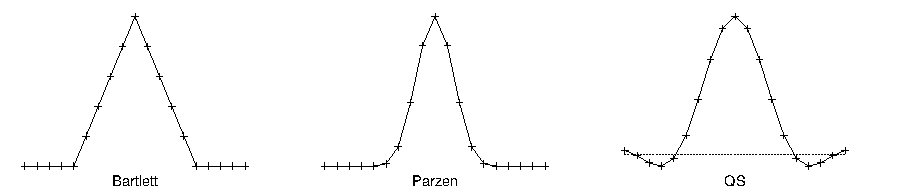
\includegraphics{figures/kernels}
\end{figure}

In \app{gretl} � possibile scegliere il kernel usando il comando \texttt{set}
col parametro \verb|hac_kernel|:
%
\begin{code}
set hac_kernel parzen
set hac_kernel qs
set hac_kernel bartlett
\end{code}

\subsection{Scelta della larghezza di banda HAC}
\label{sec:hac-bw}

La teoria asintotica sviluppata da Newey, West ed altri ci dice in termini
generali come la larghezza di banda HAC, $p$, deve crescere in relazione
all'ampiezza campionaria, $T$, ossia dice che $p$ dovrebbe crescere
proporzionalmente a qualche potenza frazionaria di $T$. Purtroppo questo non �
di molto aiuto quando nella pratica si ha a che fare con un dataset di ampiezza
fissa. Sono state suggerite varie regole pratiche, due delle quali sono
implementate da \app{gretl}. L'impostazione predefinita � $p = 0.75 T^{1/3}$,
come raccomandato da Stock e Watson (2003). Un'alternativa � $p =
4(T/100)^{2/9}$, come raccomandato in Wooldridge (2002b). In entrambi i casi si
prende la parte intera del risultato. Queste varianti sono chiamate
rispettivamente \texttt{nw1} e \texttt{nw2} nel contesto del comando \texttt{set} col parametro
\verb|hac_lag|. Ossia, � possibile impostare la versione data da
Wooldridge con il comando
%
\begin{code}
set hac_lag nw2
\end{code}
%
Come mostrato nella Tabella~\ref{tab:haclag} la scelta tra \texttt{nw1} e
\texttt{nw2} non causa rilevanti differenze.

\begin{table}[htbp]
  \centering
  \begin{tabular}{ccc}
    $T$ & $p$ (\texttt{nw1}) & $p$ (\texttt{nw2}) \\[4pt]
50& 	2& 	3 \\
100& 	3& 	4 \\
150& 	3& 	4 \\
200& 	4& 	4 \\
300& 	5& 	5 \\
400& 	5& 	5 \\
  \end{tabular}
\caption{Larghezza di banda HAC: confronto tra due regole pratiche}
\label{tab:haclag}
\end{table}

� anche possibile specificare un valore numerico fisso per $p$, come in
%
\begin{code}
set hac_lag 6
\end{code}
%
Inoltre � possibile impostare un valore diverso per il kernel QS (visto che
questo non deve essere necessariamente un valore intero).  Ad esempio:
%
\begin{code}
set qs_bandwidth 3.5
\end{code}


\subsection{Prewhitening e scelta della larghezza di banda basata sui dati}
\label{sec:hac-prewhiten}

Un approccio alternativo per trattare l'autocorrelazione dei residui consiste
nell'attaccare il problema da due fronti. L'intuizione alla base di questa
tecnica, nota come \emph{VAR prewhitening} (Andrews e Monahan, 1992) pu� essere
illustrata con un semplice esempio. Sia $x_t$ una serie di variabili casuali con
autocorrelazione del prim'ordine
%
\[
  x_t = \rho x_{t-1} + u_t
\]
%
Si pu� dimostrare che la varianza di lungo periodo di $x_t$ �
%
\[
  V_{LR}(x_t) = \frac{V_{LR}(u_t)}{(1-\rho)^2}
\]
%
Nella maggior parte dei casi, $u_t$ � meno autocorrelato di $x_t$,
quindi dovrebbe richiedere una minore larghezza di banda. La stima di
$V_{LR}(x_t)$ pu� quindi procedere in tre passi: (1) stimare $\rho$; (2)
ottenere una stima HAC di $\hat{u}_t = x_t - \hat{\rho} x_{t-1}$; (3)
dividere il risultato per $(1-\rho)^2$.

Applicare questo approccio al nostro problema implica stimare un'autoregressione
vettoriale (VAR) di ordine finito sulle variabili vettoriali
$\xi_t = X_t \hat{u}_t$. In generale, il VAR pu� essere di ordine qualsiasi, ma
nella maggior parte dei casi � sufficiente l'ordine 1; lo scopo non � quello di
produrre un modello preciso per $\xi_t$, ma solo quello di catturare la maggior parte
dell'autocorrelazione.  Quindi viene stimato il VAR seguente
%
\[
  \xi_t = A \xi_{t-1} + \varepsilon_t
\]
%
Una stima della matrice $X'\Omega X$ pu� essere ottenuta con
\[
  (I- \hat{A})^{-1} \hat{\Sigma}_{\varepsilon} (I- \hat{A}')^{-1}
\]
dove $\hat{\Sigma}_{\varepsilon}$ � uno stimatore HAC, applicato ai residui del
VAR.

In \app{gretl} � possibile usare il prewhitening con
%
\begin{code}
set hac_prewhiten on
\end{code}
%
Al momento non � possibile calcolare un VAR iniziale con un ordine diverso da 1.

Un ulteriore miglioramento di questo approccio consiste nello scegliere la
larghezza di banda in base ai dati. Intuitivamente, ha senso che la larghezza di
banda non tenga conto soltanto dell'ampiezza campionaria, ma anche delle
propriet� temporali dei dati (e anche del kernel scelto). Un metodo non
parametrico di scelta � stato proposto da Newey e West (1994) ed � spiegato
bene e in modo sintetico da Hall (2005). Questa opzione pu� essere abilitata in
gretl con il comando
%
\begin{code}
set hac_lag nw3
\end{code}
%
ed � abilitata in modo predefinito quando si seleziona il prewhitening, ma �
possibile modificarla utilizzando un valore numerico specifico per
\verb|hac_lag|.

Anche il metodo basato sui dati proposto da Newey--West non identifica univocamente
la larghezza di banda per una data ampiezza del campione. Il primo passo
consiste nel calcolare una serie di covarianze dei residui, e la lunghezza di
questa serie � una funzione dell'ampiezza campionaria, ma solo per un certo
multiplo scalare; ad esempio, � data da $O(T^{2/9})$ per il kernel di Bartlett.
\app{Gretl} usa un multiplo implicito pari a 1.


\section{Problemi speciali con dati panel}
\label{sec:vcv-panel}

Visto che i dati panel hanno sia caratteristiche di serie storiche sia
caratteristiche di dati cross-section, ci si pu� aspettare che in generale
la stima robusta della matrice di covarianza debba richiedere di gestire sia
l'eteroschedasticit� che l'autocorrelazione (l'approccio HAC). Inoltre ci sono
altre caratteristiche dei dati panel che richiedono attenzione particolare:
\begin{itemize}
\item La varianza del termine di errore pu� differire tra le unit�
  cross-section.
\item La covarianza degli errori tra le unit� pu� essere diversa da zero in ogni
  periodo temporale.
\item Se non si rimuove la variazione ``between'', gli errori possono esibire
  autocorrelazione, non nel senso classico delle serie storiche, ma nel senso
  che l'errore medio per l'unit� $i$ pu� essere diverso da quello per l'unit� $j$
  (questo � particolarmente rilevante quando il metodo di stima � pooled OLS).
\end{itemize}

\app{Gretl} al momento offre due stimatori robusti per la matrice di covarianza
da usare con dati panel, disponibili per modelli stimati con effetti fissi,
pooled OLS, e minimi quadrati a due stadi. Lo stimatore robusto predefinito �
quello suggerito da Arellano (2003), che � HAC a patto che il panel sia del tipo
``$n$ grande, $T$ piccolo'' (ossia si osservano molte unit� per pochi periodi).
Lo stimatore di Arellano �
\[
\hat{\Sigma}_{\rm A} = 
\left(X^{\prime}X\right)^{-1}
\left( \sum_{i=1}^n X_i^{\prime} \hat{u}_i 
    \hat{u}_i^{\prime} X_i \right)
\left(X^{\prime}X\right)^{-1}
\]
dove $X$ � la matrice dei regressori (con le medie di gruppo sottratte, nel caso
degli effetti fissi), $\hat{u}_i$ denota il vettore dei residui per l'unit� $i$,
e $n$ � il numero delle unit� cross-section. Cameron e Trivedi (2005) difendono
l'uso di questo stimatore, notando che il classico HCCME di White pu� produrre
errori standard artificialmente bassi in un contesto panel, perch� non tiene
conto dell'autocorrelazione.

Nei casi in cui l'autocorrelazione non � un problema, lo stimatore proposto da
Beck e Katz (1995) e discusso da Greene (2003, capitolo 13) pu� essere appropriato.
Questo stimatore, che tiene conto della correlazione contemporanea tra le unit�
e l'eteroschedasticit� per unit�, �
\[
\hat{\Sigma}_{\rm BK} = 
\left(X^{\prime}X\right)^{-1}
\left( \sum_{i=1}^n \sum_{j=1}^n \hat{\sigma}_{ij} X^{\prime}_iX_j \right)
\left(X^{\prime}X\right)^{-1}
\]
Le covarianze $\hat{\sigma}_{ij}$ sono stimate con
\[
\hat{\sigma}_{ij} = \frac{\hat{u}^{\prime}_i \hat{u}_j}{T}
\]
dove $T$ � la lunghezza della serie storica per ogni unit�. Beck e
Katz chiamano gli errori standard associati ``Panel-Corrected Standard
Errors'' (PCSE). Per usare questo stimatore in \app{gretl} basta eseguire
il comando
%
\begin{code}
set pcse on
\end{code}
%
Per reimpostare come predefinito lo stimatore di Arellano occorre eseguire
%
\begin{code}
set pcse off
\end{code}
%
Si noti che a prescindere dall'impostazione di \texttt{pcse}, lo stimatore
robusto non � usato a meno che non si aggiunga l'opzione \verb|--robust| ai
comandi di stima, o non si selezioni la casella ``Robusto'' nell'interfaccia
grafica.

%%% Local Variables: 
%%% mode: latex
%%% TeX-master: "gretl-guide"
%%% End: 

\chapter{Datos de Panel}
\label{chap-panel}


\section{Estructura de Panel}
\label{panel-structure}

Los datos de panel (una muestra combinada de datos de series
temporales y de secci�n cruzada) requieren un cuidado especial. He
aqu� algunas observaciones a tener en cuenta.

Consid�rese un conjunto de datos consistente en observaciones de
\emph{n} unidades de secci�n cruzada (pa�ses, provincias, personas,
etc.) durante \emph{T} periodos. Supongamos que cada observaci�n
contiene los valores de \emph{m} variables de inter�s. El conjunto de
datos est� formado entonces por \emph{mnT} valores.

Los datos deben de ordenarse ``por observaci�n'': cada fila representa
una observaci�n; cada columna contiene los valores de una variable en
particular. La matriz de datos tiene entonces \emph{nT} filas y
\emph{m} columnas. Esto deja abierta la cuesti�n de c�mo ordenar las
filas. Existen dos posibilidades.\footnote{Si no queremos diferenciar
  de manera conceptual o estad�stica entre variaciones muestrales y
  temporales, podemos ordenar las filas de modo arbitrario, pero esto
  es probablemente un derroche de datos.}

\begin{itemize}
\item Filas agrupadas por \emph{unidad}. Pi�nsese en la matriz de
  datos como si estuviera compuesta de \emph{n} bloques, cada uno con
  \emph{T} filas. El primer bloque de \emph{T} filas contiene las
  observaciones de la unidad 1 de la muestra para cada uno de los
  periodos; el siguiente bloque contiene las observaciones de la
  unidad 2 para todos los periodos; y as� sucesivamente. De hecho, la
  matriz de datos es un conjunto de datos de series temporales
  apilados verticalmente.
\item Filas agrupadas por \emph{periodo}. Pi�nsese en la matriz de
  datos como si estuviera compuesta por \emph{T} bloques, cada uno con
  \emph{n} filas. La primera de las \emph{n} filas contiene las
  observaciones de cada unidad muestral en el periodo 1; el siguiente
  bloque contiene las observaciones de todas las unidades en el
  periodo 2; y as� sucesivamente. La matriz de datos es un conjunto de
  datos de muestras de secci�n cruzada, apiladas verticalmente.
\end{itemize}

Puede utilizarse el esquema que resulte m�s conveniente. El primero es
quiz� m�s f�cil de mantener ordenado. Si se utiliza el segundo, hay
que asegurarse de que las unidades de secci�n cruzada aparezcan en el
mismo orden en cada uno de los bloques de datos de cada periodo.

En cualquiera de los dos casos se puede utilizar el campo frecuencia
en la l�nea \emph{observaciones} del archivo de cabecera de datos para
que el asunto resulte un poco m�s sencillo.

\begin{itemize}
\item \emph{Agrupados por unidades}: Establecer la frecuencia igual a
  \emph{T}. Supongamos que hay observaciones sobre 20 unidades durante
  5 periodos de tiempo. En este caso, la l�nea de observaciones m�s
  apropiada es la siguiente: \verb+5 1.1 20.5+ (l�ase: frecuencia 5,
  empezando con la observaci�n de la unidad 1, en el periodo 1, y
  finalizando con la observaci�n de la unidad 20, periodo 5).
  Entonces, por ejemplo, la observaci�n de la unidad 2 en el periodo 5
  puede ser referenciada como \verb+2.5+, y la correspondiente a la
  unidad 13 en periodo 1 como \verb+13.1+.
\item \emph{Agrupado por periodos}: Establecer la frecuencia igual a
  \emph{n}. En este caso, si hay observaciones sobre 20 unidades en
  cada uno de los 5 periodos, la l�nea de observaciones deber�a ser:
  \verb+20 1.01 5.20+ (l�ase: frecuencia 20, empezando con la
  observaci�n del periodo 1, unidad 01, y finalizando con la
  observaci�n del periodo 5, unidad 20). As�, nos referiremos a la
  observaci�n de la unidad 2, periodo 5 como \verb+5.02+.
\end{itemize}

Si se construye un conjunto de datos de panel utilizando un programa
de hoja de c�lculo para despu�s importar los datos a \app{gretl},
puede ser que el programa no reconozca, al principio, la clase
especial de los datos. Esto se puede arreglar mediante la instrucci�n
\cmd{setobs} (v�ase el \GCR) o la opci�n del men� GUI ``Muestra,
Seleccionar frecuencia, observaci�n inicial...)''.


\section{Variables ficticias}
\label{dummies}

En un estudio de panel puede que se desee construir variables
ficticias de uno o ambos tipos descritos a continuaci�n: (a) variables
ficticias como identificadores de las unidades muestrales, y (b)
variables ficticias como identificadores de los periodos de tiempo. El
primer m�todo puede utilizarse para permitir que el intercepto de la
regresi�n sea diferente en diferentes unidades, y el segundo para
permitir lo mismo en diferente periodos.

Hay dos opciones especiales para crear estas variables ficticias.  Se
encuentran dentro del men� ``Datos, A�adir variables'' en el GUI, o en
la instrucci�n \cmd{genr} en el modo lote de instrucciones, o
\app{gretlcli}.

\begin{enumerate}
\item ``variables ficticias peri�dicas'' (lote de instrucciones:
  \cmd{genr dummy}). Esta instrucci�n normalmente se utiliza para
  crear variables ficticias peri�dicas hasta la frecuencia de datos en
  los estudios de series temporales (por ejemplo un conjunto de
  variables ficticias trimestrales para ser utilizado en correcci�n
  estacional). No obstante, tambi�n funciona con datos de panel.
  N�tese que la interpretaci�n de las variables ficticias creadas
  mediante esta instrucci�n difiere dependiendo de si las filas de
  datos est�n agrupadas por unidad o por periodo. Si est�n agrupadas
  seg�n \emph{unidades} (frecuencia \emph{T}) las variables
  resultantes son \emph{variables ficticias peri�dicas} y habr� un
  n�mero \emph{T} de ellas. Por ejemplo, \verb+dummy_2+ tendr� el
  valor 1 en cada fila de datos correspondiente a una observaci�n del
  periodo 2, o 0 en caso contrario. Si est�n agrupadas seg�n
  \emph{periodos} (frecuencia \emph{n}) entonces se generaran \emph{n}
  \emph{variables ficticias unitarias}: \verb+dummy_2+ tendr� el valor
  1 en cada fila de datos asociada con la unidad muestral 2, o 0 en
  caso contrario.
\item ``Variables ficticias de panel'' (en modo consola \cmd{genr
    paneldum}). Esta instruccion crea todas las variables ficticias,
  de cada unidad y periodo, de golpe. Se supone que por defecto, las
  filas de datos est�n agrupadas por unidades. Las variables ficticias
  de cada unidad se denominan \verb+du_1+, \verb+du_2+ y as�
  sucesivamente, mientras que las variables ficticias peri�dicas se
  llaman \verb+dt_1+, \verb+dt_2+, etc. Es incorrecto utilizar la
  \verb+u+ (por unidad) y la \verb+t+ (por tiempo) en estos nombres si
  las filas de datos est�n agrupadas por periodos: su utilizaci�n
  correcta en este contexto se hace mediante \cmd{genr paneldum -o}
  (s�lo en modo lote de instrucciones).
\end{enumerate}

Si el conjunto de datos de panel contiene el a�o \verb+YEAR+ como una
de las variables, es posible crear un periodo ficticio para de escoger
alg�n a�o en particular como en este ejemplo \cmd{genr dum =
  (YEAR=1960)}. Tambi�n es posible crear variables ficticias
peri�dicas utilizando el operador de m�dulo, \verb+%+. Por
ejemplo, para crear una variable ficticia con valor 1 para la primera
observaci�n y cada treinta observaciones y 0 en lo dem�s casos, se
puede hacer lo siguiente

\begin{code}
  genr index genr dum = ((index-1)%30) = 0
\end{code}


\section{Uso de valores retardados con datos de panel}
\label{panel-lagged}

Si los periodos de tiempo est�n divididos en intervalos regulares,
quiz� queramos usar los valores retardados de las variables en una
regresi�n de panel. En este caso es preferible agrupar las filas de
datos por \emph{unidades} (series temporales apiladas).

Supongamos que creamos un retardo de la variable \verb+x1+, utilizando
\verb+genr x1_1 = x1(-1)+.  Los valores de esta variable ser�n en
general correctos, pero en los l�mites de los bloques de datos de cada
unidad son `` utilizables'': el valor ``previo'' no es realmente el
primer retardo de \verb+x1_1+, si no m�s bien la �ltima observaci�n de
\verb+x1+ para la unidad muestral previa.  \app{Gretl} marca estos
valores como ausentes.

Si hay que incluir un retardo de este tipo en una regresi�n, hay que
asegurarse de que la primera observaci�n de cada bloque o unidad no
est� incluida. Un modo de hacer esto es mediante M�nimos Cuadrados
Ponderados (\cmd{wls}) utilizando una variable ficticia apropiada como
ponderaci�n. Esta variable ficticia (vamos a denominarla \cmd{lagdum})
debe tener el valor 0 para las observaciones a descartar, y 1 en el
caso contrario. Es decir, es complementaria a una variable para el
periodo 1. De este modo, si hemos utilizado la instrucci�n\cmd{ genr
  dummy} podemos teclear \verb+genr lagdum = 1 - dummy_1+.  En caso de
que hubi�ramos utilizado \cmd{genr paneldum} ahora tendr�amos que
teclear \verb+genr lagdum = 1 - dt_1+.  De cualquier manera, la
siguiente instrucci�n ser�a

\verb+wls lagdum y const x1_1+ ...

para obtener una regresi�n combinada utilizando el primer retardo de
\verb+x1+, descartando todas las observaciones del periodo 1.

Otra opci�n es utilizar \cmd{smpl} con la marca \cmd{-o} y una
variable ficticia apropiada. El Ejemplo \ref{examp-pwt} muestra unas
instrucciones de ejemplo, suponiendo que cada bloque de datos de cada
unidad contiene 30 observaciones y queremos descartar la primera fila
de cada uno. Podemos entonces ejecutar las regresiones sobre el
conjunto de datos restringido sin tener que usar la instrucci�n
\cmd{wls}. Si se desea reutilizar el conjunto de datos restringido,
podemos guardarlo mediante la instrucci�n \cmd{store} (v�ase el \GCR).

\begin{script}[htbp]
  \caption{Retardos con datos de panel}
  \label{examp-panel-lags}
\begin{code}
  # crear la variable �ndice
  genr index 
  # crear dum = 0 para cada 30 observaciones 
  genr dum = ((index-1)%30) > 0
  # establecer la muestra por medio de esa variable ficticia
  smpl dum --dummy
  # crear de nuevo la estructura de observaciones, para 56 unidades
  setobs 29 1.01 56.29
\end{code}
\end{script}


\section{Estimaci�n combinada}
\label{pooled-est}

Llegados a este punto, podemos revelar que hay una instrucci�n de
estimaci�n con el prop�sito especial de ser utilizado con datos de
panel, la opci�n ``MCO combinados'' en el men� \textsf{Modelo}. Esta
instrucci�n s�lo est� disponible cuando se reconoce el conjunto de
datos como un panel. Para aprovechar esta opci�n, es preciso
especificar un modelo que no contenga ninguna variable ficticia para
representar unidades de secci�n cruzada. La rutina presenta
estimaciones sencillas de MCO combinadas, que tratan de igual manera
las variaciones de secci�n cruzada y de series temporales. Este modelo
puede que sea el apropiado o no. En el men� \textsf{Contrastes} en la
ventana de modelo, se encuentra una opci�n llamada ``Diagn�sticos de
panel'', la cual plantea el contraste de MCO combinados contra las
principales alternativas, es decir, los modelos de efectos fijos o de
efectos aleatorios.

El modelo de efectos fijos a�ade una variable ficticia a todas menos
una de las unidades de secci�n cruzada, permitiendo que var�e el
intercepto de la regresi�n en cada unidad. Se presenta un contraste
\emph{F} para la significaci�n conjunta de estas variables ficticias:
si el valor p para este contraste es peque�o, entonces se rechaza la
hip�tesis nula (de que un simple modelo combinado es adecuado) en
favor de un modelo de efectos fijos.

Por otro lado, el modelo de efectos aleatorios descompone la varianza
residual en dos partes, una parte espec�fica a la unidad de secci�n
cruzada o ``grupo'' y la otra espec�fica a una observaci�n en
particular. (Este estimador s�lo puede calcularse cuando el panel es
lo suficientemente ``amplio'', es decir, cuando el n�mero de unidades
de secci�n cruzada en el conjunto de datos excede el n�mero de
par�metros a estimar.) El contraste LM de Breusch-Pagan comprueba la
hip�tesis nula (una vez m�s, de que el estimador de MCO combinados es
adecuado) contra la alternativa de efectos aleatorios.

Cabe dentro de lo posible que el modelo MCO combinados sea rechazado
contra las dos alternativas de efectos fijos y aleatorios. Entonces la
pregunta es, �c�mo podemos valorar los m�ritos relativos de los
estimadores alternativos? El contraste de Hausman (tambi�n incluido en
el informe, siempre que el modelo de efectos aleatorios se pueda
estimar) intenta resolver este problema. El estimador de efectos
aleatorios es m�s eficiente que el estimador de efectos fijos, siempre
y cuando el error especifico a la unidad o grupo no est�
correlacionado con las variables independientes; si no es as�, el
estimador de efectos aleatorios es inconsistente, en cuyo caso es
preferible el estimador de efectos fijos. La hip�tesis nula para el
contraste de Hausman dice que el error especifico al grupo no esta tan
correlacionado (y por lo tanto es preferible el modelo de efectos
aleatorios). Por lo tanto, un valor p peque�o para este contraste
supone rechazar el modelo de efectos aleatorios en favor del modelo de
efectos fijos.

Para una discusi�n m�s rigurosa sobre este tema, v�ase Greene (2000),
cap�tulo 14.


\section{Ilustraci�n: La Tabla Mundial de Penn}
\label{PWT}

La Tabla Mundial de Penn (Penn World Table) (direcci�n
\href{http://pwt.econ.upenn.edu/}{pwt.econ.upenn.edu}) es un excelente
conjunto de datos macroecon�micos de panel, que incluye datos sobre
152 pa�ses entre los a�os 1950-1992. Los datos est�n disponibles en
formato \app{gretl}; v�ase el sitio web de datos de \app{gretl}
\url{http://gretl.sourceforge.net/gretl_data.html} (se puede descargar
gratuitamente, aunque no est� incluido en el paquete principal de
\app{gretl}).

El Ejemplo \ref{examp-pwt} de abajo abre \verb+pwt56_60_89.gdt+, un
conjunto parcial de la pwt que contiene datos sobre 120 pa�ses, entre
los a�os 1960-89, para 20 variables, sin que haya ninguna observaci�n
ausente (el conjunto de datos completo, que tambi�n est� incluido en
el paquete pwt para \app{gretl}, contiene muchas observaciones con
valores ausentes). El total de crecimiento del PIB real, entre
1960-89, se calcula para cada pa�s y se regresa contra el nivel real
del PIB en 1960, para ver si hay indicios de ``convergencia'' (es
decir, crecimiento m�s r�pido en los pa�ses que empezaron con el nivel
m�s bajo).

\begin{script}[htbp]
  \caption{Uso de la tabla mundial de Penn}
  \label{examp-pwt}
\begin{code}
  open pwt56_60_89.gdt 
  # para 1989 (�ltima observaci�n), el retardo 29 da 1960, 
  # la primera observaci�n 
  genr gdp60 = RGDPL(-29) 
  # encontrar el crecimiento total del PNB total durante 30 a�os
  genr gdpgro = (RGDPL - gdp60)/gdp60 
  # restringir la muestra a la secci�n cruzada de a�o 1989 
  smpl -r YEAR=1989 
  # �Hay convergencia?  �los pa�ses con una base menor, 
  # crecieron mas r�pido?   
  ols gdpgro const gdp60 
  # resultado: �No! Intentar la relaci�n inversa 
  genr gdp60inv = 1/gdp60 
  ols gdpgro const gdp60inv 
  # No otra vez.  �Intentar prescindir de Africa? 
  genr afdum = (CCODE = 1) genr
  afslope = afdum * gdp60 
  ols gdpgro const afdum gdp60 afslope
\end{code}
\end{script}

\chapter{Dynamic panel models}
\label{chap-dpanel}

\newcommand{\by}{\mathbf{y}}
\newcommand{\bx}{\mathbf{x}}
\newcommand{\bv}{\mathbf{v}}
\newcommand{\bX}{\mathbf{X}}
\newcommand{\bW}{\mathbf{W}}
\newcommand{\bZ}{\mathbf{Z}}
\newcommand{\biota}{\bm{\iota}}

\DefineVerbatimEnvironment%
{code}{Verbatim}
{fontsize=\small, xleftmargin=1em}

\newenvironment%
{altcode}%
{\vspace{1ex}\small\leftmargin 1em}{\vspace{1ex}}

As of \textsf{gretl} version 1.9.2, the primary command for estimating
dynamic panel models is \texttt{dpanel}. The closely related
\texttt{arbond} command has been available for some time, and is still
present, but whereas \texttt{arbond} only supports the so-called
``difference'' estimator \citep{arellano-bond91}, \texttt{dpanel} is
addition offers the ``system'' estimator \citep{blundell-bond98},
which has become the method of choice in the applied literature.

\section{Introduction}
\subsection{Notation}
\label{sec:notation}

A dynamic linear panel data model can be represented as follows
(in notation based on \cite{arellano03}):
\begin{equation}
  \label{eq:dpd-def}
  y_{it} = \alpha y_{i,t-1} + \beta'x_{it} + \eta_{i} + v_{it}
\end{equation}

The main idea on which the difference estimator is based is to get rid
of the individual effect via differencing:\footnote{An alternative is
  ``orthogonal deviations'': this is implemented in \texttt{arbond},
  but not in \texttt{dpanel}, since it was a lot of work and OD is
  very rarely seen in the wild.} first-differencing
eq.\ (\ref{eq:dpd-def}) yields
\begin{equation}
  \label{eq:dpd-dif}
  \Delta y_{it} = \alpha \Delta y_{i,t-1} + \beta'\Delta x_{it} +
  \Delta v_{it} = \gamma' W_{it} + \Delta v_{it} ,
\end{equation}
in obvious notation. The error term of (\ref{eq:dpd-dif}) is, by
construction, autocorrelated and also correlated with the lagged
dependent variable, so an estimator that takes both issues into
account is needed. The endogeneity issue is solved by noting that all
values of $y_{i,t-k}$, with $k>1$ can be used as instruments for
$\Delta y_{i,t-1}$: unobserved values of $y_{i,t-k}$ (because they
could be missing, or pre-sample) can safely be substituted with 0. In
the language of GMM, this amounts to using the relation
\begin{equation}
  \label{eq:OC-dif}
  E(\Delta v_{it} \cdot y_{i,t-k}) = 0, \quad k>1
\end{equation}
as an orthogonality condition.

Autocorrelation is dealt with by noting that, if $v_{it}$ is a white
noise, then the covariance matrix of the vector whose typical element
is $\Delta v_{it}$ is proportional to a matrix $H$ that has 2 on the
main diagonal, $-1$ on the first subdiagonals and 0 elsewhere. In
practice, one-step GMM estimation of equation (\ref{eq:dpd-dif})
amounts to computing
\begin{align}
  \hat{\gamma} = & \left[ 
    \left( \sum_{i=1}^N \bW_i'\bZ_i \right)
    \left( \sum_{i=1}^N \bZ_i' H \bZ_i \right)^{-1}
    \left( \sum_{i=1}^N \bZ_i'\bW_i \right)
      \right]^{-1} \times \notag \\
    \times & \left( \sum_{i=1}^N \bW_i'\bZ_i \right)
    \left( \sum_{i=1}^N \bZ_i' H \bZ_i \right)^{-1}
    \left( \sum_{i=1}^N \bZ_i'\Delta \by_i \right) \label{eq:dif-gmm}
\end{align}
where
\begin{eqnarray*}
  \Delta \by_i  & = &
     \left[ \begin{array}{ccc}
         \Delta y_{i,3} & \cdots & \Delta y_{i,T}
       \end{array} \right]' \\
  \bW_i  & = &
     \left[ \begin{array}{ccc}
         \Delta y_{i,2} & \cdots & \Delta y_{i,T-1} \\
         \Delta x_{i,3} & \cdots & \Delta x_{i,T} \\
       \end{array} \right]' \\
  \bZ_i  & = &
     \left[ \begin{array}{ccccccc}
         y_{i1} & 0 & 0 & \cdots & 0 & \Delta x_{i3}\\
         0 & y_{i1} & y_{i2} & \cdots & 0 & \Delta x_{i4}\\
         & & \vdots \\
         0 & 0 & 0 & \cdots & y_{i, T-2} & \Delta x_{iT} \\
       \end{array} \right]' 
\end{eqnarray*}
Once the 1-step estimator is computed, the sample covariance matrix of
the estimated residuals can be used instead of $H$ to obtain 2-step
estimates, which are not only consistent but asymptotically
efficient.\footnote{In theory, the process may be iterated, but nobody
  seems to be interested.} Standard GMM theory applies, except for
one thing: \cite{Windmeijer05} has computed finite-sample corrections to the
asymptotic covariance matrix of the parameters, which are nowadays
almost universally used.

The difference estimator is consistent, but has been shown to have
poor properties in finite samples when $\alpha$ is near one. People
these days prefer the so-called ``system'' estimator, which
complements the differenced data (with lagged levels used as
instruments) with data in levels (using lagged differences as
instruments). The system estimator relies on an extra orthogonality
condition which has to do with the earliest value of the dependent
variable $y_{i,1}$. The interested reader is referred to
\citet[pp.\ 124--125]{blundell-bond98} for details, but here it suffices
to say that this condition is satisfied in mean-stationary models and
brings about efficiency that may be substantial in many cases.

The set of orthogonality conditions exploited in the system approach
is not very much larger than with the difference estimator,
the reason being that most of the possible orthogonality conditions
associated with the equations in levels are redundant, given those
already used for the equations in differences.

The key equations of the system estimator can be written as

\begin{align}
  \tilde{\gamma} = & \left[ 
    \left( \sum_{i=1}^N \tilde{\bW}'\tilde{\bZ} \right)
    \left( \sum_{i=1}^N \tilde{\bZ}' H^* \tilde{\bZ} \right)^{-1}
    \left( \sum_{i=1}^N \tilde{\bZ}'\tilde{\bW} \right)
      \right]^{-1} \times \notag \\
    \times & \left( \sum_{i=1}^N \tilde{\bW}'\tilde{\bZ} \right)
    \left( \sum_{i=1}^N \tilde{\bZ}' H^* \tilde{\bZ} \right)^{-1}
    \left( \sum_{i=1}^N \tilde{\bZ}'\Delta \tilde{\by}_i \right)  \label{eq:sys-gmm}
\end{align}
where
\begin{eqnarray*}
  \Delta \tilde{\by}_i  & = &
     \left[ \begin{array}{ccccccc}
         \Delta y_{i3} & \cdots & \Delta y_{iT} & y_{i3} & \cdots & y_{iT}
       \end{array} \right]' \\
  \tilde{\bW}_i  & = &
     \left[ \begin{array}{cccccc}
         \Delta y_{i2} & \cdots & \Delta y_{i,T-1} & y_{i2} & \cdots & y_{i,T-1} \\
         \Delta x_{i3} & \cdots & \Delta x_{iT}  & x_{i3} & \cdots & x_{iT} \\
       \end{array} \right]' \\
  \tilde{\bZ}_i  & = &
     \left[ \begin{array}{ccccccccc}
         y_{i1} & 0 & 0       & \cdots & 0  & 0  & \cdots & 0 & \Delta x_{i,3}\\
         0 & y_{i1} & y_{i2} & \cdots & 0  & 0  & \cdots & 0 & \Delta x_{i,4}\\
         & & \vdots \\
         0 & 0 & 0 & \cdots & y_{i, T-2} & 0  & \cdots & 0  & \Delta x_{iT}\\
         & & \vdots \\
         0 & 0 & 0 & \cdots & 0 & \Delta y_{i2} & \cdots & 0  & x_{i3}\\
         & & \vdots \\
         0 & 0 & 0 & \cdots & 0 & 0 & \cdots & \Delta y_{i,T-1}  & x_{iT}\\
       \end{array} \right]' 
\end{eqnarray*}

In this case choosing a precise form for the matrix $H^*$ for the
first step is no trivial matter. Its north-west block should be as
similar as possible to the covariance matrix of the vector $\Delta
v_{it}$, so the same choice as the ``difference'' estimator is
appropriate. Ideally, the south-east block should be proportional to
the covariance matrix of the vector $\biota \eta_i + \bv$, that is
$\sigma^2_{v} I + \sigma^2_{\eta} \biota \biota'$; but since
$\sigma^2_{\eta}$ is unknown and any positive definite matrix renders
the estimator consistent, people just use $I$. The off-diagonal blocks
should, in principle, contain the covariances between $\Delta v_{is}$
and $v_{it}$, which would be an identity matrix if $v_{it}$ is white
noise. However, since the south-east block is typically given a
conventional value anyway, the benefit in making this choice is not
obvious. Some packages use $I$; others use a zero matrix.
Asymptotically, it should not matter, but on real datasets the
difference between the resulting estimates can be noticeable.

\subsection{Rank deficiency}
\label{sec:rankdef}

Both the difference estimator (\ref{eq:dif-gmm}) and the system
estimator (\ref{eq:sys-gmm}) depend, for their existence, on the
invertibility of $A = \sum_{i=1}^N \tilde{\bZ}' H^* \tilde{\bZ}$. This
matrix may turn out to be singular for several reasons. However, this
does not mean that the estimator is not computable: in some cases,
adjustments are possible such that the estimator does exist, but the
user must be aware that in these cases not all software packages use
the same strategy and replication of results may prove difficult or
even impossible.

A first reason why $A$ may be singular could be the unavailability of
instruments, chiefly because of missing observations. This case is
easy to handle. If a particular row of $\tilde{\bZ}_i$ is zero for all
units, the corresponding orthogonality condition (or the corresponding
instrument if you prefer) is automatically dropped; of course, the
overidentification rank is adjusted for testing purposes.

Even if no instruments are zero, however, $A$ could be rank
deficient. A trivial case occurs if there are collinear instruments,
but a less trivial case may arise when $T$ (the total number of time
periods available) is not much smaller than $N$ (the number of units),
as, for example, in some macro datasets where the units are
countries. The total number of potentially usable orthogonality
conditions is $O(T^2)$, which may well exceed $N$ in some cases. Of
course $A$ is the sum of $N$ matrices which have, at most, rank $2T -
3$ and therefore it could well happen that $A$ is singular.

In all these cases, what we consider the ``proper'' way to go is to
substitute the pseudo-inverse of $A$ (Moore--Penrose) for its regular
inverse. Again, our choice is shared by some software packages, but
not all, so replication may be hard.


\subsection{Treatment of missing values}

Textbooks seldom bother with missing values, but in some cases their
treatment may be far from obvious. This is especially true if missing
values are interspersed between valid observations. For example,
consider the plain difference estimator with one lag, so
\[
y_t = \alpha y_{t-1} + \eta + \epsilon_t
\]
where the $i$ index is omitted for clarity. Suppose you have an
individual with $t=1\ldots5$, for which $y_3$ is missing. It may seem
that the data for this individual are unusable, because
differencing $y_t$ would produce something like
\[
\begin{array}{c|ccccc}
  t & 1 & 2 & 3 & 4 & 5 \\
  \hline
  y_t & * & * & \circ & * & * \\
  \Delta y_t & \circ & * & \circ & \circ & *
\end{array}
\]
where $*$ = nonmissing and $\circ$ = missing. Estimation seems to be
unfeasible, since there are no periods in which $\Delta y_t$ and
$\Delta y_{t-1}$ are both observable.

However, we can use a $k$-difference operator and get
\[
\Delta_k y_t = \alpha \Delta_k y_{t-1} + \Delta_k \epsilon_t
\]
where $\Delta_k = 1 - L^k$ and past levels of $y_t$ are perfectly
valid instruments. In this example, we can choose $k=3$ and use $y_1$
as an instrument, so this unit is in fact perfectly usable.

Not all software packages seem to be aware of this possibility, so
replicating published results may prove tricky if your dataset
contains individuals with ``gaps'' between valid observations.

\section{Usage}

One of the concepts underlying the syntax of \texttt{dpanel} is that
you get default values for several choices you may want to make, so
that in a ``standard'' situation the command itself is very short to
write (and read).  The simplest case of the model (\ref{eq:dpd-def})
is a plain AR(1) process:
\begin{equation}
\label{eq:dp1}
  y_{i,t} = \alpha y_{i,t-1} + \eta_{i} + v_{it} .
\end{equation}
If you give the command
\begin{code}
  dpanel 1 ; y
\end{code}
gretl assumes that you want to estimate (\ref{eq:dp1}) via the
difference estimator (\ref{eq:dif-gmm}), using as many orthogonality
conditions as possible.  The scalar \texttt{1} between \texttt{dpanel}
and the semicolon indicates that only one lag of \texttt{y} is
included as an explanatory variable; using \texttt{2} would give an
AR(2) model. The syntax that gretl uses for the non-seasonal AR and MA
lags in an ARMA model is also supported in this context.\footnote{This
  represents an enhancement over the \texttt{arbond} command.} For
example, if you want the first and third lags of \texttt{y} (but not
the second) included as explanatory variables you can say
\begin{code}
  dpanel {1 3} ; y
\end{code}
or you can use a pre-defined matrix for this purpose:
\begin{code}
  matrix ylags = {1, 3}
  dpanel ylags ; y
\end{code}
To use a single lag of \texttt{y} other than the first you need to
employ this mechanism:
\begin{code}
  dpanel {3} ; y # only lag 3 is included
  dpanel 3 ; y   # compare: lags 1, 2 and 3 are used
\end{code}

To use the system estimator instead, you add the \verb|--system|
option, as in
\begin{code}
  dpanel 1 ; y --system
\end{code}
The level orthogonality conditions and the corresponding instrument
are appended automatically (see eq.\ \ref{eq:sys-gmm}).

\subsection{Regressors}

If we want to introduce additional regressors, we list them after
the dependent variable in the same way as other \texttt{gretl}
commands, such as \texttt{ols}. 

For the difference orthogonality relations, \texttt{dpanel} takes care
of transforming the regressors in parallel with the dependent
variable. Note that this differs from gretl's \texttt{arbond} command,
where only the dependent variable is differenced automatically; it
brings us more in line with other software.

One case of potential ambiguity is when an intercept is specified but
the difference-only estimator is selected, as in
\begin{code}
  dpanel 1 ; y const
\end{code}
In this case the default \texttt{dpanel} behavior, which agrees with
Stata's \texttt{xtabond2}, is to drop the constant (since differencing
reduces it to nothing but zeros). However, for compatibility with the
DPD package for Ox, you can give the option \verb|--dpdstyle|, in
which case the constant is retained (equivalent to including a linear
trend in equation~\ref{eq:dpd-def}).  A similar point applies to the
period-specific dummy variables which can be added in \texttt{dpanel}
via the \verb|--time-dummies| option: in the differences-only case
these dummies are entered in differenced form by default, but when the
\verb|--dpdstyle| switch is applied they are entered in levels.

The standard \texttt{gretl} syntax applies if you want to use lagged
explanatory variables, so for example the command
\begin{code}
  dpanel 1 ; y const x(0 to -1) --system
\end{code}
would result in estimation of the model
\[
  y_{it} = \alpha y_{i,t-1} + 
  \beta_0 + \beta_1 x_{it} + \beta_2 x_{i,t-1} +
  \eta_{i} + v_{it} .
\]


\subsection{Instruments}

The default rules for instruments are: 
\begin{itemize}
\item lags of the dependent variable are instrumented using all
  available orthogonality conditions; and
\item additional regressors are considered exogenous, so they are used
  as their own instruments.
\end{itemize}

If a different policy is wanted, the instruments should be specified
in an additional list, separated from the regressors list by a
semicolon. The syntax closely mirrors that for the \texttt{tsls}
command, but in this context it is necessary to distinguish between
``regular'' instruments and what are often called ``GMM-style''
instruments (that, instruments that are handled in the same
block-diagonal manner as lags of the dependent variable, as described
above).

``Regular'' instruments are transformed in the same way as
regressors, and the contemporaneous value of the transformed variable
is used to form an orthogonality condition. Since regressors are
treated as exogenous by default, it follows that these two commands
estimate the same model:

\begin{code}
  dpanel 1 ; y z
  dpanel 1 ; y z ; z
\end{code}
The instrument specification in the second case simply confirms what
is implicit in the first: that \texttt{z} is exogenous. Note, though,
that if you have some additional variable \texttt{z2} which you want
to add as a regular instrument, it then becomes necessary to 
include \texttt{z} in the instrument list if it is to be treated
as exogenous:
\begin{code}
  dpanel 1 ; y z ; z2   # z is now implicitly endogenous
  dpanel 1 ; y z ; z z2 # z is treated as exogenous
\end{code}

The specification of ``GMM-style'' instruments is handled by the
special constructs \texttt{GMM()} and \texttt{GMMlevel()}.  The first
of these relates to instruments for the equations in differences, and
the second to the equations in levels. The syntax for \texttt{GMM()}
is

\begin{altcode}
\texttt{GMM(}\textsl{varname}\texttt{,} \textsl{minlag}\texttt{,} 
\textsl{maxlag}\texttt{)}
\end{altcode}

\noindent
where \textsl{varname} is replaced by the name of a series,
and \textsl{minlag} and \textsl{maxlag} are replaced by the minimum
and maximum lags to be used as instruments. The same goes for 
\texttt{GMMlevel()}.

One common use of \texttt{GMM()} is to limit the number of lagged
levels of the dependent variable used as instruments for the equations
in differences. It's well known that although exploiting all possible
orthogonality conditions yields maximal asymptotic efficiency, in
finite samples it may be preferable to use a smaller subset (but see
also \cite{OkuiJoE2009}).  For example, the specification

\begin{code}
  dpanel 1 ; y ; GMM(y, 2, 4)
\end{code}
ensures that no lags of $y_t$ earlier than $t-4$ will be used as
instruments.

A second use of \texttt{GMM()} is to exploit more fully the potential
block-diagonal orthogonality conditions offered by an exogenous
regressor, or a related variable that does not appear as a regressor.
For example, in

\begin{code}
  dpanel 1 ; y x ; GMM(z, 2, 6)
\end{code}
the variable \texttt{x} is considered an endogenous regressor, and up to
5 lags of \texttt{z} are used as instruments.

Note that in the following script fragment
\begin{code}
  dz = diff(z)
  dpanel 1 ; y dz
  dpanel 1 ; y dz ; GMM(z,0,0)
\end{code}
the two estimation commands should not be expected to give the same
result, as the sets of orthogonality relationships are subtly
different.  In the latter case, you have $T-2$ separate orthogonality
relationships pertaining to $z_{it}$, none of which has any
implication for the other ones; in the former case, you only have one.
In terms of the $\bZ_i$ matrix, the first form adds a single row to
the bottom of the instruments matrix, while the second form adds a
diagonal block with $T-2$ columns, that is
\[
  \left[ \begin{array}{cccc}
         \Delta z_{i3} & \Delta z_{i4} & \cdots & \Delta z_{it}
       \end{array} \right]
\] 
versus
\[
  \left[ \begin{array}{cccc}
         \Delta z_{i3} & 0 & \cdots & 0 \\
         0 & \Delta z_{i4} & \cdots & 0 \\
          & \ddots & \ddots &  \\
         0 & 0 & \cdots & \Delta z_{it} 
       \end{array} \right]
\]

\section{Replication of DPD results}
\label{sec:DPD-replic}

In this section we show how to replicate the results of some of the
pioneering work with dynamic panel-data estimators by Arellano, Bond
and Blundell.  As the DPD manual \citep*{DPDmanual} explains, it is
difficult to replicate the original published results exactly, for two
main reasons: not all of the data used in those studies are publicly
available; and some of the choices made in the original software
implementation of the estimators have been superseded.  Here,
therefore, our focus is on replicating the results obtained using the
current DPD package and reported in the DPD manual.

The examples are based on the program files \texttt{abest1.ox},
\texttt{abest3.ox} and \texttt{bbest1.ox}. These are included in the
DPD package, along with the Arellano--Bond database files
\texttt{abdata.bn7} and \texttt{abdata.in7}.\footnote{See
  \url{http://www.doornik.com/download.html}.} The
Arellano--Bond data are also provided with gretl, in the file
\texttt{abdata.gdt}. In the following we do not show the output from
DPD or gretl; it is somewhat voluminous, and is easily generated by
the user. As of this writing the results from Ox/DPD and gretl are
identical in all relevant respects for all of the examples
shown.\footnote{To be specific, this is using Ox Console version 5.10,
  version 1.24 of the DPD package, and gretl built from CVS as of
  2010-10-23, all on Linux.}

A complete Ox/DPD program to generate the results of interest takes
this general form:

\begin{code}
#include <oxstd.h>
#import <packages/dpd/dpd>

main()
{
    decl dpd = new DPD();

    dpd.Load("abdata.in7");
    dpd.SetYear("YEAR");

    // model-specific code here

    delete dpd;
}
\end{code}
%
In the examples below we take this template for granted and show just
the model-specific code.

\subsection{Example 1}

The following Ox/DPD code---drawn from \texttt{abest1.ox}---replicates
column (b) of Table 4 in \cite{arellano-bond91}, an instance of the
differences-only or GMM-DIF estimator. The dependent variable is the
log of employment, \texttt{n}; the regressors include two lags of the
dependent variable, current and lagged values of the log real-product
wage, \texttt{w}, the current value of the log of gross capital,
\texttt{k}, and current and lagged values of the log of industry
output, \texttt{ys}. In addition the specification includes a constant
and five year dummies; unlike the stochastic regressors, these
deterministic terms are not differenced. In this specification the
regressors \texttt{w}, \texttt{k} and \texttt{ys} are treated as
exogenous and serve as their own instruments. In DPD syntax this
requires entering these variables twice, on the \verb|X_VAR| and
\verb|I_VAR| lines. The GMM-type (block-diagonal) instruments in this
example are the second and subsequent lags of the level of \texttt{n}.
Both 1-step and 2-step estimates are computed.

\begin{code}
dpd.SetOptions(FALSE); // don't use robust standard errors
dpd.Select(Y_VAR, {"n", 0, 2});
dpd.Select(X_VAR, {"w", 0, 1, "k", 0, 0, "ys", 0, 1});
dpd.Select(I_VAR, {"w", 0, 1, "k", 0, 0, "ys", 0, 1});

dpd.Gmm("n", 2, 99);
dpd.SetDummies(D_CONSTANT + D_TIME);

print("\n\n***** Arellano & Bond (1991), Table 4 (b)");
dpd.SetMethod(M_1STEP);
dpd.Estimate();
dpd.SetMethod(M_2STEP);
dpd.Estimate();
\end{code}

Here is gretl code to do the same job:

\begin{code}
open abdata.gdt
list X = w w(-1) k ys ys(-1)
dpanel 2 ; n X const --time-dummies --asy --dpdstyle
dpanel 2 ; n X const --time-dummies --asy --two-step --dpdstyle
\end{code}

Note that in gretl the switch to suppress robust standard errors is
\verb|--asymptotic|, here abbreviated to \verb|--asy|.\footnote{Option
  flags in gretl can always be truncated, down to the minimal unique
  abbreviation.} The \verb|--dpdstyle| flag specifies that the
constant and dummies should not be differenced, in the context of a
GMM-DIF model. With gretl's \texttt{dpanel} command it is not
necessary to specify the exogenous regressors as their own instruments
since this is the default; similarly, the use of the second and all
longer lags of the dependent variable as GMM-type instruments is the
default and need not be stated explicitly. 

\subsection{Example 2}

The DPD file \texttt{abest3.ox} contains a variant of the above that
differs with regard to the choice of instruments: the variables
\texttt{w} and \texttt{k} are now treated as predetermined, and are
instrumented GMM-style using the second and third lags of their
levels. This approximates column (c) of Table 4 in
\cite{arellano-bond91}.  We have modified the code in
\texttt{abest3.ox} slightly to allow the use of robust
(Windmeijer-corrected) standard errors, which are the default in both
DPD and gretl with 2-step estimation:

\begin{code}
dpd.Select(Y_VAR, {"n", 0, 2});
dpd.Select(X_VAR, {"w", 0, 1, "k", 0, 0, "ys", 0, 1});
dpd.Select(I_VAR, {"ys", 0, 1});
dpd.SetDummies(D_CONSTANT + D_TIME);

dpd.Gmm("n", 2, 99);
dpd.Gmm("w", 2, 3);
dpd.Gmm("k", 2, 3);

print("\n***** Arellano & Bond (1991), Table 4 (c)\n");
print("        (but using different instruments!!)\n");
dpd.SetMethod(M_2STEP);
dpd.Estimate();
\end{code}

The gretl code is as follows:

\begin{code}
open abdata.gdt
list X = w w(-1) k ys ys(-1)
list Ivars = ys ys(-1)
dpanel 2 ; n X const ; GMM(w,2,3) GMM(k,2,3) Ivars --time --two-step --dpd
\end{code}
%
Note that since we are now calling for an instrument set other then
the default (following the second semicolon), it is necessary to
include the \texttt{Ivars} specification for the variable \texttt{ys}.
However, it is not necessary to specify \texttt{GMM(n,2,99)} since
this remains the default treatment of the dependent variable.

\subsection{Example 3}

Our third example replicates the DPD output from \texttt{bbest1.ox}:
this uses the same dataset as the previous examples but the model
specifications are based on \cite{blundell-bond98}, and involve
comparison of the GMM-DIF and GMM-SYS (``system'') estimators. The
basic specification is slightly simplified in that the variable
\texttt{ys} is not used and only one lag of the dependent variable
appears as a regressor. The Ox/DPD code is:

\begin{code}
dpd.Select(Y_VAR, {"n", 0, 1});
dpd.Select(X_VAR, {"w", 0, 1, "k", 0, 1});
dpd.SetDummies(D_CONSTANT + D_TIME);

print("\n\n***** Blundell & Bond (1998), Table 4: 1976-86 GMM-DIF");
dpd.Gmm("n", 2, 99);
dpd.Gmm("w", 2, 99);
dpd.Gmm("k", 2, 99);
dpd.SetMethod(M_2STEP);
dpd.Estimate();

print("\n\n***** Blundell & Bond (1998), Table 4: 1976-86 GMM-SYS");
dpd.GmmLevel("n", 1, 1);
dpd.GmmLevel("w", 1, 1);
dpd.GmmLevel("k", 1, 1);
dpd.SetMethod(M_2STEP);
dpd.Estimate();
\end{code}

Here is the corresponding gretl code:

\begin{code}
open abdata.gdt
list X = w w(-1) k k(-1)

# Blundell & Bond (1998), Table 4: 1976-86 GMM-DIF
dpanel 1 ; n X const ; GMM(w,2,99) GMM(k,2,99) --time --two-step --dpd

# Blundell & Bond (1998), Table 4: 1976-86 GMM-SYS
dpanel 1 ; n X const ; GMM(w,2,99) GMM(k,2,99) \
  GMMlevel(w,1,1) GMMlevel(k,1,1) --time --two-step --dpd --system
\end{code}

Note the use of the \verb|--system| option flag to specify GMM-SYS,
including the default treatment of the dependent variable, which
corresponds to \texttt{GMMlevel(n,1,1)}. In this case we also want to
use lagged differences of the regressors \texttt{w} and \texttt{k} as
instruments for the levels equations so we need explicit
\texttt{GMMlevel} entries for those variables. If you want something
other than the default treatment for the dependent variable as an
instrument for the levels equations, you should give an explicit
\texttt{GMMlevel} specification for that variable---and in that case
the \verb|--system| flag is redundant (but harmless).

For the sake of completeness, note that if you specify at least one
\texttt{GMMlevel} term, \texttt{dpanel} will then include equations in
levels, but it will not automatically add a default \texttt{GMMlevel}
specification for the dependent variable unless the \verb|--system|
option is given.

\section{Cross-country growth example}
\label{sec:dpanel-growth}

The previous examples all used the Arellano--Bond dataset; for this
example we use the dataset \texttt{CEL.gdt}, which is also included in
the gretl distribution. As with the Arellano--Bond data, there are
numerous missing values.  Details of the provenance of the data can be
found by opening the dataset information window in the gretl GUI
(\textsf{Data} menu, \textsf{Dataset info} item). This is a subset of
the Barro--Lee 138-country panel dataset, an approximation to which is
used in \citet*{CEL96} and \citet*{Bond2001}.\footnote{We say an
  ``approximation'' because we have not been able to replicate exactly
  the OLS results reported in the papers cited, though it seems from
  the description of the data in \cite{CEL96} that we ought to be able
  to do so.  We note that \cite{Bond2001} used data provided by
  Professor Caselli yet did not manage to reproduce the latter's
  results.}  Both of these papers explore the dynamic panel-data
approach in relation to the issues of growth and convergence of per
capita income across countries.

The dependent variable is growth in real GDP per capita over
successive five-year periods; the regressors are the log of the
initial (five years prior) value of GDP per capita, the log-ratio of
investment to GDP, $s$, in the prior five years, and the log of annual
average population growth, $n$, over the prior five years plus 0.05 as
stand-in for the rate of technical progress, $g$, plus the rate of
depreciation, $\delta$ (with the last two terms assumed to be constant
across both countries and periods).  The original model is
\begin{equation}
\label{eq:CEL96}
\Delta_5 y_{it} = \beta y_{i,t-5} + \alpha s_{it} + \gamma (n_{it} +
g + \delta) + \nu_t + \eta_i + \epsilon_{it}
\end{equation}
which allows for a time-specific disturbance $\nu_t$. The Solow model
with Cobb--Douglas production function implies that $\gamma =
-\alpha$, but this assumption is not imposed in estimation. The
time-specific disturbance is eliminated by subtracting the period mean
from each of the series.

Equation (\ref{eq:CEL96}) can be transformed to an AR(1) dynamic
panel-data model by adding $y_{i,t-5}$ to both sides, which gives
\begin{equation}
\label{eq:CEL96a}
y_{it} = (1 + \beta) y_{i,t-5} + \alpha s_{it} + \gamma (n_{it} +
g + \delta) + \eta_i + \epsilon_{it}
\end{equation}
where all variables are now assumed to be time-demeaned.

In (rough) replication of \cite{Bond2001} we now proceed to estimate
the following two models: (a) equation (\ref{eq:CEL96a}) via GMM-DIF,
using as instruments the second and all longer lags of $y_{it}$,
$s_{it}$ and $n_{it} + g + \delta$; and (b) equation
(\ref{eq:CEL96a}) via GMM-SYS, using $\Delta y_{i,t-1}$, $\Delta
s_{i,t-1}$ and $\Delta (n_{i,t-1} + g + \delta)$ as additional
instruments in the levels equations. We report robust standard errors
throughout. (As a purely notational matter, we now use ``$t-1$'' to
refer to values five years prior to $t$, as in \cite{Bond2001}).

The gretl script to do this job is shown below. Note that the final
transformed versions of the variables (logs, with time-means
subtracted) are named \texttt{ly} ($y_{it}$), \texttt{linv} ($s_{it}$)
and \texttt{lngd} ($n_{it} + g + \delta$).
%
\begin{code}
open CEL.gdt

ngd = n + 0.05
ly = log(y)
linv = log(s)
lngd = log(ngd)

# take out time means
loop i=1..8 --quiet
  smpl (time == i) --restrict --replace
  ly -= mean(ly)
  linv -= mean(linv)
  lngd -= mean(lngd)
endloop

smpl --full
list X = linv lngd
# 1-step GMM-DIF
dpanel 1 ; ly X ; GMM(linv,2,99) GMM(lngd,2,99)
# 2-step GMM-DIF
dpanel 1 ; ly X ; GMM(linv,2,99) GMM(lngd,2,99) --two-step
# GMM-SYS
dpanel 1 ; ly X ; GMM(linv,2,99) GMM(lngd,2,99) \
 GMMlevel(linv,1,1) GMMlevel(lngd,1,1) --two-step --sys
\end{code}

For comparison we estimated the same two models using Ox/DPD and the
Stata command \texttt{xtabond2}. (In each case we constructed a
comma-separated values dataset containing the data as transformed in
the gretl script shown above, using a missing-value code appropriate
to the target program.) For reference, the commands used with
Stata are reproduced below:
%
\begin{code}
insheet using CEL.csv
tsset unit time
xtabond2 ly L.ly linv lngd, gmm(L.ly, lag(1 99)) gmm(linv, lag(2 99)) 
  gmm(lngd, lag(2 99)) rob nolev
xtabond2 ly L.ly linv lngd, gmm(L.ly, lag(1 99)) gmm(linv, lag(2 99)) 
  gmm(lngd, lag(2 99)) rob nolev twostep
xtabond2 ly L.ly linv lngd, gmm(L.ly, lag(1 99)) gmm(linv, lag(2 99)) 
  gmm(lngd, lag(2 99)) rob nocons twostep
\end{code}

For the GMM-DIF model all three programs find 382 usable observations
and 30 instruments, and yield identical parameter estimates and
robust standard errors (up to the number of digits printed, or more);
see Table~\ref{tab:growth-DIF}.\footnote{The coefficient shown for
  \texttt{ly(-1)} in the Tables is that reported directly by the
  software; for comparability with the original model (eq.\
  \ref{eq:CEL96}) it is necesary to subtract 1, which produces the
  expected negative value indicating conditional convergence in per
  capita income.}

\begin{table}[htbp]
\begin{center}
\begin{tabular}{lrrrr}
& \multicolumn{2}{c}{1-step} & \multicolumn{2}{c}{2-step} \\
& \multicolumn{1}{c}{coeff} & \multicolumn{1}{c}{std.\ error} &
  \multicolumn{1}{c}{coeff} & \multicolumn{1}{c}{std.\ error} \\
\texttt{ly(-1)} & 0.577564 & 0.1292 & 0.610056 & 0.1562 \\
\texttt{linv} & 0.0565469 & 0.07082 & 0.100952 & 0.07772 \\
\texttt{lngd} & $-$0.143950 & 0.2753 & $-$0.310041 & 0.2980 \\
\end{tabular}
\caption{GMM-DIF: Barro--Lee data}
\label{tab:growth-DIF}
\end{center}
\end{table}

Results for GMM-SYS estimation are shown in
Table~\ref{tab:growth-SYS}. In this case we show two sets of gretl
results: those labeled ``gretl(1)'' were obtained using gretl's
\verb|--dpdstyle| option, while those labeled ``gretl(2)'' did not use
that option---the intent being to reproduce the $H$ matrices used by
Ox/DPD and \texttt{xtabond2} respectively.

\begin{table}[htbp]
\begin{center}
\begin{tabular}{lrrrr}
& \multicolumn{1}{c}{gretl(1)} & 
  \multicolumn{1}{c}{Ox/DPD} &
  \multicolumn{1}{c}{gretl(2)} & 
  \multicolumn{1}{c}{xtabond2} \\
\texttt{ly(-1)} & 0.9237 (0.0385) & 
  0.9167 (0.0373) & 
    0.9073 (0.0370) &
      0.9073 (0.0370) \\
\texttt{linv} & 0.1592 (0.0449) & 
  0.1636 (0.0441) & 
    0.1856 (0.0411) &
      0.1856 (0.0411) \\
\texttt{lngd} & $-$0.2370 (0.1485) & 
  $-$0.2178 (0.1433) & 
    $-$0.2355 (0.1501) &
      $-$0.2355 (0.1501) 
\end{tabular}
\caption{2-step GMM-SYS: Barro--Lee data (standard errors in parentheses)}
\label{tab:growth-SYS}
\end{center}
\end{table}

In this case all three programs use 479 observations; gretl and
\texttt{xtabond2} use 41 instruments and produce the same estimates
(when using the same $H$ matrix) while Ox/DPD nominally uses
66.\footnote{This is a case of the issue described in
  section~\ref{sec:rankdef}: the full $A$ matrix turns out to be
  singular and special measures must be taken to produce estimates.}
It is noteworthy that with GMM-SYS plus ``messy'' missing
observations, the results depend on the precise array of instruments
used, which in turn depends on the details of the implementation of
the estimator.

\subsection*{Auxiliary test statistics}

We have concentrated above on the parameter estimates and standard
errors. It may be worth adding a few words on the additional test
statistics that typically accompany both GMM-DIF and GMM-SYS
estimation. These include the Sargan test for overidentification, one
or more Wald tests for the joint significance of the regressors, and time
dummies if applicable, and tests for first- and second-order
autocorrelation of the residuals from the equations in differences.

In general we see a good level of agreement between gretl, DPD and
\texttt{xtabond2} with regard to these statistics, with a few
relatively minor exceptions. Specifically, \texttt{xtabond2} computes
both a ``Sargan test'' and a ``Hansen test'' for overidentification,
but what it calls the Hansen test is what DPD and gretl call the
Sargan test. (We have had difficulty determining from the
\texttt{xtabond2} documentation \citep{Roodman2006} exactly how its
Sargan test is computed.) In addition there are cases where the
degrees of freedom for the Sargan test differ between DPD and gretl;
this occurs when the $A$ matrix is singular
(section~\ref{sec:rankdef}). In concept the df equals the number of
instruments minus the number of parameters estimated; for the first of
these terms gretl uses the rank of $A$, while DPD appears to use the
full dimension of $A$.

\section{Memo: \texttt{dpanel} options}
\label{sec:options}

\begin{center}
\begin{tabular}{lp{.7\textwidth}}
  \textit{flag} & \textit{effect} \\ [6pt]
  \verb|--asymptotic| & Suppresses the use of robust standard errors \\
  \verb|--two-step| & Calls for 2-step estimation (the default being 1-step) \\
  \verb|--system| & Calls for GMM-SYS, with default treatment of the 
  dependent variable, as in \texttt{GMMlevel(y,1,1)} \\
  \verb|--time-dummies| & Includes period-specific dummy variables \\
  \verb|--dpdstyle| & Compute the $H$ matrix as in DPD; also suppresses
  differencing of automatic time dummies and omission of intercept
  in the GMM-DIF case\\
  \verb|--verbose| & When \verb|--two-step| is selected, prints 
  the 1-step estimates first \\
  \verb|--vcv| & Calls for printing of the covariance matrix \\
  \verb|--quiet| & Suppresses the printing of results \\
\end{tabular}
\end{center}



\chapter{Nonlinear least squares}
\label{chap-nls}

\section{Introduction and examples}
\label{nls-intro}

\app{Gretl} supports nonlinear least squares (NLS) using a variant of
the Levenberg--Marquardt algorithm.  The user must supply a
specification of the regression function; prior to giving this
specification the parameters to be estimated must be ``declared'' and
given initial values.  Optionally, the user may supply analytical
derivatives of the regression function with respect to each of the
parameters.  If derivatives are not given, the user must instead give
a list of the parameters to be estimated (separated by spaces or
commas), preceded by the keyword \cmd{params}.  The tolerance
(criterion for terminating the iterative estimation procedure) can be
adjusted using the \cmd{set} command.

The syntax for specifying the function to be estimated is the same as
for the \cmd{genr} command.  Here are two examples, with accompanying
derivatives.

\begin{code}
# Consumption function from Greene
nls C = alpha + beta * Y^gamma
    deriv alpha = 1
    deriv beta = Y^gamma
    deriv gamma = beta * Y^gamma * log(Y)
end nls

# Nonlinear function from Russell Davidson
nls y = alpha + beta * x1 + (1/beta) * x2
    deriv alpha = 1
    deriv beta = x1 - x2/(beta*beta)
end nls --vcv
\end{code}

Note the command words \cmd{nls} (which introduces the regression
function), \cmd{deriv} (which introduces the specification of a
derivative), and \cmd{end nls}, which terminates the specification and
calls for estimation. If the \cmd{--vcv} flag is appended to the last
line the covariance matrix of the parameter estimates is printed.

\section{Initializing the parameters}
\label{nls-param}

The parameters of the regression function must be given initial values
prior to the \cmd{nls} command.  This can be done using the \cmd{genr}
command (or, in the GUI program, via the menu item ``Variable, Define new
variable'').  

In some cases, where the nonlinear function is a generalization of (or
a restricted form of) a linear model, it may be convenient to run an
\cmd{ols} and initialize the parameters from the OLS coefficient
estimates.  In relation to the first example above, one might do:
%
\begin{code}
ols C 0 Y
genr alpha = $coeff(0)
genr beta = $coeff(Y)
genr gamma = 1
\end{code}

And in relation to the second example one might do:
%
\begin{code}
ols y 0 x1 x2
genr alpha = $coeff(0)
genr beta = $coeff(x1)
\end{code}


\section{NLS dialog window}
\label{nls-gui}

It is probably most convenient to compose the commands for NLS
estimation in the form of a \app{gretl} script but you can also do so
interactively, by selecting the item ``Nonlinear Least Squares'' under
the ``Model, Nonlinear models'' menu.  This opens a dialog box where you can
type the function specification (possibly prefaced by \cmd{genr} lines to set
the initial parameter values) and the derivatives, if available.  An
example of this is shown in Figure~\ref{fig-nls-dialog}.  Note that in
this context you do not have to supply the \cmd{nls} and \cmd{end nls}
tags.

\begin{figure}[htbp]
  \begin{center}
    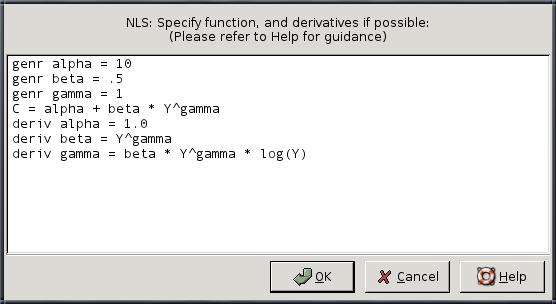
\includegraphics[scale=0.5]{figures/nls_window}
  \end{center}
  \caption{NLS dialog box}
  \label{fig-nls-dialog}
\end{figure}


\section{Analytical and numerical derivatives}
\label{nls-deriv}

If you are able to figure out the derivatives of the regression
function with respect to the parameters, it is advisable to supply
those derivatives as shown in the examples above.  If that is not
possible, \app{gretl} will compute approximate numerical derivatives.
However, the properties of the NLS algorithm may not be so good in
this case (see section~\ref{nls-accuracy}).

This is done by using the \cmd{params} statement, which should be
followed by a list of identifiers containing the parameters to be
estimated. In this case, the examples above would read as follows:

\begin{code}
# Greene
nls C = alpha + beta * Y^gamma
    params alpha beta gamma
end nls
\end{code}

\begin{code}
# Davidson
nls y = alpha + beta * x1 + (1/beta) * x2
    params alpha beta
end nls
\end{code}

If analytical derivatives are supplied, they are checked for
consistency with the given nonlinear function.  If the derivatives are
clearly incorrect estimation is aborted with an error message.  If the
derivatives are ``suspicious'' a warning message is issued but
estimation proceeds.  This warning may sometimes be triggered by
incorrect derivatives, but it may also be triggered by a high degree
of collinearity among the derivatives.

Note that you cannot mix analytical and numerical derivatives: you
should supply expressions for all of the derivatives or none.

\section{Controlling termination}
\label{nls-toler}

The NLS estimation procedure is an iterative process.  Iteration is
terminated when the criterion for convergence is met or when the
maximum number of iterations is reached, whichever comes first.

Let $k$ denote the number of parameters being estimated.  The maximum
number of iterations is $100 \times (k+1)$ when analytical derivatives
are given, and $200 \times (k+1)$ when numerical derivatives are used.

Let $\epsilon$ denote a small number.  The iteration is deemed to have
converged if at least one of the following conditions is satisfied:

\begin{itemize}
\item Both the actual and predicted relative reductions in the error
  sum of squares are at most $\epsilon$.
\item The relative error between two consecutive iterates is at most
  $\epsilon$.
\end{itemize}

This default value of $\epsilon$ is the machine precision to the power
3/4,\footnote{On a 32-bit Intel Pentium machine a likely value for
  this parameter is $1.82\times 10^{-12}$.} but it can be adjusted
using the \cmd{set} command with the parameter \verb+nls_toler+.  For
example
%
\begin{code}
set nls_toler .0001
\end{code}
% 
will relax the value of $\epsilon$ to 0.0001.

\section{Details on the code}
\label{nls-code}

The underlying engine for NLS estimation is based on the \app{minpack}
suite of functions, available from
\href{http://www.netlib.org/minpack/}{netlib.org}.  Specifically, the
following \app{minpack} functions are called:

\begin{center}
  \begin{tabular}{ll}
    \verb+lmder+ & Levenberg--Marquardt algorithm with analytical
    derivatives
    \\
    \verb+chkder+ & Check the supplied analytical derivatives
    \\
    \verb+lmdif+ & Levenberg--Marquardt algorithm with numerical
    derivatives
    \\
    \verb+fdjac2+ & Compute final approximate Jacobian when using
    numerical derivatives
    \\
    \verb+dpmpar+ & Determine the machine precision
    \\
  \end{tabular}
\end{center}

On successful completion of the Levenberg--Marquardt iteration, a
Gauss--Newton regression is used to calculate the covariance matrix
for the parameter estimates.  If the \option{robust} flag is given a
robust variant is computed.  The documentation for the \cmd{set}
command explains the specific options available in this regard.

Since NLS results are asymptotic, there is room for debate over
whether or not a correction for degrees of freedom should be applied
when calculating the standard error of the regression (and the
standard errors of the parameter estimates).  For comparability with
OLS, and in light of the reasoning given in
\cite{davidson-mackinnon93}, the estimates shown in \app{gretl}
\emph{do} use a degrees of freedom correction.

\section{Numerical accuracy}
\label{nls-accuracy}

Table \ref{tab-nls} shows the results of running the \app{gretl} NLS
procedure on the 27 Statistical Reference Datasets made available by
the U.S.  National Institute of Standards and Technology (NIST) for
testing nonlinear regression software.\footnote{For a discussion of
  \app{gretl}'s accuracy in the estimation of linear models, see
  Appendix~\ref{app-accuracy}.}  For each dataset, two sets of
starting values for the parameters are given in the test files, so the
full test comprises 54 runs.  Two full tests were performed, one using
all analytical derivatives and one using all numerical approximations.
In each case the default tolerance was used.\footnote{The data shown
  in the table were gathered from a pre-release build of \app{gretl}
  version 1.0.9, compiled with \app{gcc} 3.3, linked against
  \app{glibc} 2.3.2, and run under Linux on an i686 PC (IBM ThinkPad
  A21m).}

Out of the 54 runs, \app{gretl} failed to produce a solution
in 4 cases when using analytical derivatives, and in 5 cases when
using numeric approximation. Of the four failures in analytical
derivatives mode, two were due to non-convergence of the
Levenberg--Marquardt algorithm after the maximum number of iterations
(on \verb+MGH09+ and \verb+Bennett5+, both described by NIST as of
``Higher difficulty'') and two were due to generation of range errors
(out-of-bounds floating point values) when computing the Jacobian (on
\verb+BoxBOD+ and \verb+MGH17+, described as of ``Higher difficulty''
and ``Average difficulty'' respectively).  The additional failure in
numerical approximation mode was on \verb+MGH10+ (``Higher
difficulty'', maximum number of iterations reached).

The table gives information on several aspects of the tests: the
number of outright failures, the average number of iterations taken to
produce a solution and two sorts of measure of the accuracy of the
estimates for both the parameters and the standard errors of the
parameters.

For each of the 54 runs in each mode, if the run produced a solution
the parameter estimates obtained by \app{gretl} were compared with the
NIST certified values.  We define the ``minimum correct figures'' for
a given run as the number of significant figures to which the
\emph{least accurate} \app{gretl} estimate agreed with the certified
value, for that run. The table shows both the average and the worst
case value of this variable across all the runs that produced a
solution.  The same information is shown for the estimated standard
errors.\footnote{For the standard errors, I excluded one outlier from
  the statistics shown in the table, namely \verb+Lanczos1+.  This is
  an odd case, using generated data with an almost-exact fit: the
  standard errors are 9 or 10 orders of magnitude smaller than the
  coefficients.  In this instance \app{gretl} could reproduce the
  certified standard errors to only 3 figures (analytical derivatives)
  and 2 figures (numerical derivatives).}  

The second measure of accuracy shown is the percentage of cases,
taking into account all parameters from all successful runs, in which
the \app{gretl} estimate agreed with the certified value to at least
the 6 significant figures which are printed by default in the
\app{gretl} regression output.

\begin{table}[htbp]
 \caption{Nonlinear regression: the NIST tests}
 \label{tab-nls}
  \begin{center}
    \begin{tabular}{lcc}
      � & \textit{Analytical derivatives} & 
          \textit{Numerical derivatives} \\ [4pt]
        Failures in 54 tests & 4 & 5\\
        Average iterations & 32 & 127\\
        Mean of min. correct figures, & 8.120 & 6.980\\
        parameters \\
        Worst of min. correct figures, & 4 & 3\\
        parameters \\
        Mean of min. correct figures, & 8.000 & 5.673\\
        standard errors \\
        Worst of min. correct figures, & 5 & 2\\
        standard errors \\
        Percent correct to at least 6 figures, & 96.5 & 91.9\\
        parameters \\
        Percent correct to at least 6 figures, & 97.7 & 77.3\\
        standard errors \\
      \end{tabular}
    \end{center}
  \end{table}

  Using analytical derivatives, the worst case values for both
  parameters and standard errors were improved to 6 correct figures on
  the test machine when the tolerance was tightened to 1.0e$-$14.
  Using numerical derivatives, the same tightening of the tolerance
  raised the worst values to 5 correct figures for the parameters and
  3 figures for standard errors, at a cost of one additional failure
  of convergence.

  Note the overall superiority of analytical derivatives: on average
  solutions to the test problems were obtained with substantially
  fewer iterations and the results were more accurate (most notably
  for the estimated standard errors).  Note also that the six-digit
  results printed by \app{gretl} are not 100 percent reliable for
  difficult nonlinear problems (in particular when using numerical
  derivatives).  Having registered this caveat, the percentage of
  cases where the results were good to six digits or better seems high
  enough to justify their printing in this form.

%%% Local Variables: 
%%% mode: latex
%%% TeX-master: "gretl-guide"
%%% End: 

\chapter{Stima di massima verosimiglianza}
\label{chap:mle}

\section{Stima di massima verosimiglianza con gretl}

La stima di massima verosimiglianza (maximum likelihood, ML) � una pietra
angolare delle procedure moderne di inferenza. Gretl fornisce un modo per
implementare questa metodologia per un grande numero di problemi di stima,
usando il comando \texttt{mle}.  Seguono alcuni esempi.

\subsection{Introduzione}
\label{sec:background}
Per illustrare gli esempi seguenti, inizieremo con un breve ripasso degli
aspetti basilari della stima di massima verosimiglianza. Dato un campione di
ampiezza $T$, � possibile definire la funzione di densit�\footnote{Stiamo
  supponendo che i nostri dati siano una realizzazione di variabili casuali
  continue. Per variabili discrete, la trattazione rimane valida, riferendosi
  alla funzione di probabilit� invece che a quella di densit�. In entrambi i
  casi, la distribuzione pu� essere condizionale su alcune variabili esogene.}
per l'intero campione, ossia la distribuzione congiunta di tutte le
osservazioni $f(\mathbf{Y} ; \theta)$, dove $\mathbf{Y} =
\left\{ y_1, \ldots, y_T \right\}$.  La sua forma � determinata da un $k$-vettore di
parametri sconosciuti $\theta$, che assumiamo contenuti in un insieme $\Theta$,
e che possono essere usati per stimare la probabilit� di osservare un campione
con qualsiasi data caratteristica.

Dopo aver osservato i dati, i valori di $\mathbf{Y}$ sono noti, e questa
funzione pu� essere valutata per tutti i possibili valori di $\theta$. Quando
usiamo $y_t$ come argomento e $\theta$ come parametro, la funzione �
interpretabile come una densit�, mentre � preferibile chiamarla funzione di
\emph{verosimiglianza} quando $\theta$ � considerato argomento della funzione
e i valori dei dati $\mathbf{Y}$ hanno il solo compito di determinarne la forma.

Nei casi pi� comuni, questa funzione possiede un massimo unico, la cui posizione
non viene alterata dal fatto di considerare il logaritmo della verosimiglianza
(ossia la log-verosimiglianza): questa funzione si esprime come
\[
  \LogLik(\theta) = \log  f(\mathbf{Y}; \theta)
\] 
Le funzioni di log-verosimiglianza gestite da gretl sono quelle in cui
$\LogLik(\theta)$ pu� essere scritta come
\[
  \LogLik(\theta) = \sum_{t=1}^T \ell_t(\theta)
\] 
che � vero nella maggior parte dei casi di interesse. Le funzioni
$\ell_t(\theta)$ vengono chiamate contributi di log-verosimiglianza.

Inoltre, la posizione del massimo � ovviamente determinata dai dati
$\mathbf{Y}$. Ci� significa che il valore
\begin{equation}
  \label{eq:maxlik}
  \hat{\theta}(\mathbf{Y}) = \stackunder{\theta \in \Theta}{\mathrm{Argmax}} \LogLik(\theta)
\end{equation}
� una qualche funzione dei dati osservati (ossia una statistica), che ha la
propriet�, sotto alcune condizioni deboli, di essere uno stimatore consistente,
asintoticamente normale e asintoticamente efficiente, di $\theta$.

In alcuni casi � possibile scrivere esplicitamente la funzione
$\hat{\theta}(\mathbf{Y})$, ma in generale ci� non � sempre vero, e il massimo
va cercato con tecniche numeriche. Queste si basano spesso sul fatto che la
log-verosimiglianza � una funzione continuamente differenziabile di $\theta$, e
quindi nel massimo le sue derivate parziali devono essere tutte pari a 0.
Il \textsl{vettore gradiente}, o \textsl{vettore degli score}, � una funzione
con molte propriet� interessanti dal punto di vista
statistico, che verr� denotata con $\mathbf{g}(\theta)$.
� un $k$-vettore con elemento tipico
\[
g_i(\theta) = \frac{\partial\LogLik(\theta)}{\partial\theta_i} 
  = \sum_{t=1}^T \frac{\partial\ell_t(\theta)}{\partial\theta_i}
\]


I metodi basati sul gradiente possono essere illustrati brevemente:

\begin{enumerate}
\item scegliere un punto $\theta_0 \in \Theta$;
\item valutare $\mathbf{g}(\theta_0)$;
\item se $\mathbf{g}(\theta_0)$ � ``piccolo'', fermarsi; altrimenti calcolare
  un vettore di direzione $d(\mathbf{g}(\theta_0))$;
\item valutare $\theta_1 = \theta_0 + d(\mathbf{g}(\theta_0))$;
\item sostituire $\theta_0$ con $\theta_1$;
\item ricominciare dal punto 2.
\end{enumerate}

Esistono molti algoritmi di questo tipo; si differenziano nel modo con cui
calcolano il vettore di direzione
$d(\mathbf{g}(\theta_0))$, per assicurarsi che sia $\LogLik(\theta_1) >
\LogLik(\theta_0)$ (in modo che prima o poi si arrivi a un massimo).

Il metodo usato da \app{gretl} per massimizzare la log-verosimiglianza � un algoritmo
basato sul gradiente, noto come metodo di \textbf{BFGS} (Broyden,
Fletcher, Goldfarb e Shanno). Questa tecnica � usata in molti pacchetti
statistici ed econometrici, visto che � ritenuta valida e molto potente.
Ovviamente, per rendere operativa questa tecnica, deve essere possibile
calcolare il vettore $\mathbf{g}(\theta)$ per ogni valore di $\theta$.  In
alcuni casi, la funzione $\mathbf{g}(\theta)$ pu� essere vista esplicitamente in
termini di $\mathbf{Y}$. Se questo non � possibile, o � troppo difficile,
il gradiente pu� essere valutato numericamente.

La scelta del valore iniziale $\theta_0$ � cruciale in alcuni contesti e
ininfluente in altri. In generale � consigliabile far partire l'algoritmo da
valori ``sensibili'', quando � possibile. Se � disponibile uno stimatore
consistente, di solito � una scelta valida ed efficiente: ci si assicura che per
grandi campioni il punto di partenza sar� probabilmente vicino a $\hat{\theta}$
e la convergenza sar� raggiunta in poche iterazioni.
 
Il numero massimo di iterazioni consentite per la procedura BFGS, e la relativa
tolleranza per valutare la convergenza, possono essere impostati usando il
comando \cmd{set}: le variabili relative sono
\verb+bfgs_maxiter+ (valore predefinito: 500) e \verb+bfgs_toler+ (valore
predefinito: la precisione della macchina elevata alla potenza 3/4).

\subsection{Matrice di covarianza ed errori standard}

Per impostazione predefinita, la matrice delle stime dei parametri � basata sul
prodotto esterno del gradiente (OPG, Outer Product of the Gradient), ossia:
\[
\widehat{\mbox{Var}}_{\mbox{\scriptsize OPG}}(\hat{\theta}) =
  \left(G'(\hat{\theta}) G(\hat{\theta}) \right)^{-1}
\]
dove $G(\hat{\theta})$ � la matrice $T \times k$ dei contributi al
gradiente. Sono disponibili due altre possibilit�: se si usa l'opzione
\verb|--hessian|, la matrice di covarianza viene calcolata con
un'approssimazione numerica dell'Hessiana alla convergenza. Se si usa l'opzione
\verb|--robust|, viene usato lo stimatore ``sandwich'' di quasi-massima
verosimiglianza:
\[
\widehat{\mbox{Var}}_{\mbox{\scriptsize QML}}(\hat{\theta}) = H(\hat{\theta})^{-1}
  G'(\hat{\theta}) G(\hat{\theta}) H(\hat{\theta})^{-1}
\]
dove $H$ denota l'approssimazione numerica dell'Hessiana.

\section{Stima di una Gamma}
\label{sec:gamma}

Si supponga di avere un campione di $T$ osservazioni indipendenti e
identicamente distribuite da una distribuzione Gamma. La funzione di densit� per
ogni osservazione $x_t$ �
\begin{equation}
  \label{eq:gammadens}
  f(x_t) = \frac{\alpha^p}{\Gamma(p)} x_t^{p-1} \exp\left({-\alpha
      x_t}\right)
\end{equation}
La log-verosimiglianza per l'intero campione pu� essere scritta come il
logaritmo della densit� congiunta di tutte le osservazioni. Visto che queste
sono indipendenti e identiche, la densit� congiunta � il prodotto delle densit�
individuali, e quindi il suo logaritmo �
\begin{equation}
  \label{eq:gammaloglik}
  \LogLik(\alpha, p) = \sum_{t=1}^T \log \left[ \frac{\alpha^p}{\Gamma(p)} x_t^{p-1} \exp\left({-\alpha
      x_t}\right) \right] = 
      \sum_{t=1}^T \ell_t
\end{equation}
dove
\[
  \ell_t = p \cdot \log (\alpha x_t) - \gamma(p) - \log x_t - \alpha x_t
\]
e $\gamma(\cdot)$ � il logaritmo della funzione gamma.
Per stimare i parametri $\alpha$ e $p$ con la massima verosimiglianza, occorre
massimizzare (\ref{eq:gammaloglik}) rispetto ad essi. Il frammento di codice da
eseguire in \app{gretl} �

\begin{code}
scalar alpha = 1
scalar p = 1
scalar p = 1
mle logl =  p*ln(alpha * x) - lngamma(p) - ln(x) - alpha * x 
end mle 
\end{code}

I due comandi

\begin{code}
alpha = 1
p = 1
\end{code}

sono necessari per assicurarsi che le variabili \texttt{p} e \texttt{alpha}
esistano prima di tentare il calcolo di \texttt{logl}. Il loro valore sar�
modificato dall'esecuzione del comando \texttt{mle} e sar� sostituito dalle
stime di massima verosimiglianza se la procedura � andata a buon fine. Il valore
iniziale � 1 per entrambi; � arbitrario e non conta molto in questo esempio (ma
si veda oltre).

Il codice visto pu� essere reso pi� leggibile, e leggermente pi� efficiente,
definendo una variabile in cui memorizzare $\alpha \cdot x_t$. Questo comando
pu� essere inserito nel blocco \texttt{mle} nel modo seguente:
\begin{code}
scalar alpha = 1
scalar p = 1
scalar p = 1
mle logl =  p*ln(ax) - lngamma(p) - ln(x) - ax 
series ax = alpha*x
params alpha p
end mle 
\end{code}
In questo caso, � necessario includere la riga \texttt{params alpha
  p} per impostare i simboli \texttt{p} e \texttt{alpha} separatamente da
\texttt{ax}, che � una variabile generata temporaneamente, e non un parametro da
stimare.

In un semplice esempio come questo, la scelta dei valori iniziali � quasi
ininfluente, visto che l'algoritmo converger� a prescindere dai valori iniziali.
In ogni caso, stimatori consistenti basati sul metodo dei momenti
per $p$ e $\alpha$ possono essere ricavati dalla media campionaria
$m$ e dalla varianza $V$: visto che si pu� dimostrare che
\[
  E(x_t) = p/\alpha \qquad  V(x_t) = p/\alpha^2
\]
segue che gli stimatori
\begin{eqnarray*}
  \bar{\alpha} & = &  m/V \\
  \bar{p} & = & m \cdot \bar{\alpha} 
\end{eqnarray*}
sono consistenti e quindi appropriati da usare come punti di partenza per
l'algoritmo.
Lo script per \app{gretl} diventa quindi
\begin{code}
scalar m = mean(x)
scalar alpha = m/var(x)
scalar p = m*alpha
scalar p = m*alpha
mle logl =  p*ln(ax) - lngamma(p) - ln(x) - ax 
series ax = alpha*x
params alpha p
end mle 
\end{code}

Un'altro fatto di cui tener conto � che talvolta i parametri sono vincolati
all'interno di certi intervalli: in questo caso, ad esempio, sia $\alpha$
che $p$ devono essere numeri positivi. \app{Gretl} non controlla queste
condizioni: � responsabilit� dell'utente assicurarsi che la funzione venga
sempre valutata in un punto ammissibile dello spazio dei parametri, durante la
ricerca iterativa del massimo. Un metodo efficace per far questo consiste nel
definire una variabile per controllare che i parametri siano ammissibili e
impostare la log-verosimiglianza come indefinita se il controllo fallisce. Si
veda il seguente esempio, che usa l'operatore di assegnazione condizionale:
\begin{code}
scalar m = mean(x)
scalar alpha = m/var(x)
scalar p = m*alpha
scalar p = m*alpha

mle logl = check ? p*ln(ax) - lngamma(p) - ln(x) - ax : NA
  series ax = alpha*x
  scalar check = (alpha>0) & (p>0)
params alpha p
end mle 
\end{code}

\section{Funzioni di costo con frontiera stocastica}
\label{sec:frontier}

Quando si modella una funzione di costo, talvolta � utile incorporare
esplicitamente nel modello statistico il fatto che le imprese possano essere
inefficienti, cos� che il costo osservato si discosta dal valore teorico non
solo per l'eterogeneit� (non osservata) tra le imprese, ma anche perch� due
imprese, uguali sotto tutti gli aspetti, potrebbero operare a diversi regimi di
efficienza. In questo caso, possiamo scrivere
\[
  C_i = C^*_i + u_i + v_i
\]
dove $C_i$ � qualche indicatore dei costi variabili, $C_i^*$ � il suo valore
``teorico'', $u_i$ � un termine di disturbo a media zero e $v_i$ � il termine
che modella l'inefficienza, che si suppone essere non negativo, per il suo
significato.

Spesso si sceglie una specificazione lineare per $C_i^*$; ad esempio,
la funzione di costo Cobb--Douglas si ottiene quando $C_i^*$ � una
funzione lineare dei logaritmi dei prezzi degli input e delle quantit�
di output.

Il modello con \emph{frontiera stocastica} � un modello lineare del tipo
$y_i = x_i \beta + \varepsilon_i$ in cui il termine di errore
$\varepsilon_i$ � la somma di $u_i$ e $v_i$.  Un postulato tipico � che siano
$u_i \sim N(0,\sigma_u^2)$ e $v_i \sim \left|N(0,\sigma_v^2)\right|$. Se si
ipotizza anche l'indipendenza tra $u_i$ e $v_i$, � possibile dimostrare che la
funzione di densit� di $\varepsilon_i$ ha la forma:
\begin{equation}
  \label{eq:frontdens}
  f(\varepsilon_i) = 
   \sqrt{\frac{2}{\pi}} 
   \Phi\left(\frac{\lambda \varepsilon_i}{\sigma}\right)
   \frac{1}{\sigma} \phi\left(\frac{\varepsilon_i}{\sigma}\right)
\end{equation}
dove $\Phi(\cdot)$ e $\phi(\cdot)$ sono, rispettivamente, la funzione di
distribuzione e quella di densit� della normale standard, $\sigma =
\sqrt{\sigma^2_u + \sigma^2_v}$ e $\lambda = \frac{\sigma_u}{\sigma_v}$.

Di conseguenza, la log-verosimiglianza per una osservazione ha la seguente forma
(a meno di una costante non rilevante):
\[
  \ell_t = 
  \log\Phi\left(\frac{\lambda \varepsilon_i}{\sigma}\right) -
  \left[ \log(\sigma) + \frac{\varepsilon_i^2}{2 \sigma^2} \right]
\]
Quindi il modello di funzione di costo Cobb-Douglas con frontiera stocastica �
descritto dalle seguenti equazioni:

\begin{eqnarray*}
  \log C_i & = & \log C^*_i + \varepsilon_i \\
  \log C^*_i & = & c + \sum_{j=1}^m \beta_j \log y_{ij} + \sum_{j=1}^n \alpha_j \log p_{ij} \\
  \varepsilon_i & = & u_i + v_i \\
  u_i & \sim & N(0,\sigma_u^2) \\
  v_i & \sim & \left|N(0,\sigma_v^2)\right|
\end{eqnarray*}

In molti casi, si intende assicurarsi che l'omogeneit� della funzione di costo
rispetto ai prezzi sia valida per costruzione; visto che questa condizione
equivale a $\sum_{j=1}^n \alpha_j = 1$, l'equazione vista sopra per $C^*_i$
pu� essere riscritta come

\begin{equation}
  \label{eq:CobbDouglasFrontier}
  \log C_i - \log p_{in}  = c + \sum_{j=1}^m \beta_j \log y_{ij} +
  \sum_{j=2}^n \alpha_j (\log p_{ij} - \log p_{in})  + \varepsilon_i
\end{equation}

Questa equazione pu� essere stimata con OLS, ma con due inconvenienti: per prima
cosa lo stimatore OLS per l'intercetta $c$ non � consistente, perch� il termine
di disturbo ha media diversa da zero; in secondo luogo, gli stimatori OLS per
gli altri parametri sono consistenti, ma inefficienti, a causa della
non-normalit� di $\varepsilon_i$. Entrambi i problemi possono essere risolti
stimando la (\ref{eq:CobbDouglasFrontier}) con la massima verosimiglianza.
Tuttavia, la stima OLS � un modo veloce e comodo per ricavare dei valori
iniziali per l'algoritmo di massima verosimiglianza.

L'esempio \ref{cost-estimation} mostra come implementare il modello descritto
finora. Il file \texttt{banks91} contiene parte dei dati usati in
Lucchetti, Papi e Zazzaro (2001).

\begin{script}[htbp]
  \caption{Stima di una funzione di costo con frontiera stocastica}
  \label{cost-estimation}
\begin{scode}
open banks91

# Funzione di costo Cobb-Douglas

ols cost const y p1 p2 p3

# Funzione di costo Cobb-Douglas con vincoli di omogeneit�

genr rcost = cost - p3
genr rp1 = p1 - p3
genr rp2 = p2 - p3

ols rcost const y rp1 rp2

# Funzione di costo Cobb-Douglas con vincoli di omogeneit�
# e inefficienza

scalar b0 = $coeff(const)
scalar b1 = $coeff(y)
scalar b2 = $coeff(rp1)
scalar b3 = $coeff(rp2)

scalar su = 0.1
scalar sv = 0.1

mle logl = ln(cnorm(e*lambda/ss)) - (ln(ss) + 0.5*(e/ss)^2)
  scalar ss = sqrt(su^2 + sv^2)
  scalar lambda = su/sv
  series e = rcost - b0*const - b1*y - b2*rp1 - b3*rp2
  params b0 b1 b2 b3 su sv
end mle
\end{scode}
\end{script}

\section{Modelli GARCH}
\label{sec:garch}

Gretl gestisce i modelli GARCH attraverso una funzione interna, tuttavia pu�
essere istruttivo vedere come possono essere stimati usando il comando
\texttt{mle}.

Le equazioni seguenti mostrano l'esempio pi� semplice di modello GARCH(1,1):
\begin{eqnarray*}
  y_t & = & \mu + \varepsilon_t \\
  \varepsilon_t & = & u_t \cdot \sigma_t \\
  u_t & \sim & N(0,1) \\
  h_t & = & \omega + \alpha \varepsilon^2_{t-1} + \beta h_{t-1}.
\end{eqnarray*}
Poich� la varianza di $y_t$ dipende dai valori passati, per scrivere la funzione
di log-verosimiglianza non basta sommare i logaritmi delle densit� per le
singole osservazioni. Come spesso accade nei modelli di serie storiche, $y_t$
non pu� essere considerato indipendente dalle altre osservazioni del campione,
di conseguenza, la funzione di densit� per l'intero campione (la densit�
congiunta di tutte le osservazioni) non � semplicemente il prodotto delle
densit� marginali.

La stima di massima verosimiglianza, in questi casi, si effettua considerando le
densit� \emph{condizionali}, quindi quello che si massimizza � una funzione di
verosimiglianza condizionale. Se definiamo il set informativo al tempo $t$ come
\[
  F_t = \left\{ y_t, y_{t-1}, \ldots \right\} ,
\]
la densit� di $y_t$ condizionata a $F_{t-1}$ � normale:
\[
  y_t | F_{t-1} \sim N\left[ \mu, h_{t} \right].
\]

Per le propriet� delle distribuzioni condizionali, la densit� congiunta pu�
essere fattorizzata nel modo seguente
\[
  f(y_t, y_{t-1}, \ldots) = \left[ \prod_{t=1}^T f(y_t |F_{t-1})
  \right] \cdot f(y_0)
\]
Se trattiamo $y_0$ come fissato, il termine $f(y_0)$ non dipende dai parametri
sconosciuti, e quindi la log-verosimiglianza condizionale pu� essere scritta
come la somma dei contributi individuali
\begin{equation}
  \label{eq:garchloglik}
  \LogLik(\mu,\omega,\alpha,\beta) = \sum_{t=1}^T \ell_t
\end{equation}
dove 
\[
  \ell_t = \log \left[ \frac{1}{\sqrt{h_t}} \phi\left( \frac{y_t - \mu}{\sqrt{h_t}}
    \right) \right] = 
    - \frac{1}{2} \left[ \log(h_t) + \frac{(y_t - \mu)^2}{h_t} \right]
\]

Lo script seguente mostra una semplice applicazione di questa tecnica, che usa
il file di dati \texttt{djclose}, uno dei dataset di esempio forniti con gretl,
che contiene dati giornalieri per l'indice azionario Dow Jones.

\begin{code}
open djclose

series y = 100*ldiff(djclose)

scalar mu = 0.0
scalar omega = 1
scalar alpha = 0.4
scalar beta = 0.0

mle ll = -0.5*(log(h) + (e^2)/h)
  series e = y - mu
  series h = var(y)
  series h = omega + alpha*(e(-1))^2 + beta*h(-1)
  params mu omega alpha beta
end mle
\end{code}

\section{Derivate analitiche}
\label{sec:anal-der}

Il calcolo del vettore degli score � essenziale per lavorare col metodo BFGS.
In tutti gli esempi precedenti non � stata data alcuna formula esplicita per il
calcolo dello score, ma sono stati indicati all'algoritmo dei gradienti valutati
numericamente. Il calcolo numerico dello score per il parametro
$i$-esimo � effettuato tramite un'approssimazione finita della derivata, ossia
\[
  \pder{\LogLik(\theta_1, \ldots, \theta_n)}{\theta_i} \simeq 
  \frac{\LogLik(\theta_1, \ldots, \theta_i + h, \ldots, \theta_n) -
    \LogLik(\theta_1, \ldots, \theta_i - h, \ldots, \theta_n)}{2h}
\]
dove $h$ � un numero piccolo.

In molte situazioni questo metodo � abbastanza efficiente e accurato, ma
potrebbe esserci la necessit� di evitare le approssimazioni e specificare una
funzione esatta per le derivate. Come esempio, si consideri lo script seguente:
%
\begin{code}
nulldata 1000

genr x1 = normal()
genr x2 = normal()
genr x3 = normal()

genr ystar = x1 + x2 + x3 + normal()
genr y = (ystar > 0)

scalar b0 = 0
scalar b1 = 0
scalar b2 = 0
scalar b3 = 0

mle logl = y*ln(P) + (1-y)*ln(1-P)
  series ndx = b0 + b1*x1 + b2*x2 + b3*x3
  series P = cnorm(ndx)
  params b0 b1 b2 b3
end mle --verbose
\end{code}

Vengono generate artificialmente 1000 osservazioni per un modello probit
ordinario\footnote{Ancora una volta ricordiamo che gretl contiene il comando
  interno \texttt{probit} (si veda il capitolo \ref{sec:logit-probit}), ma in
  questo caso usiamo il modello probit come
  esempio per la procedura}: $y_t$ � una variabile binaria, che assume valore 1 se
$y_t^* = \beta_1 x_{1t} + \beta_2 x_{2t} + \beta_3 x_{3t} +
\varepsilon_t > 0$ e 0 altrove. Quindi, $y_t = 1$ con probabilit�
$\Phi(\beta_1 x_{1t} + \beta_2 x_{2t} + \beta_3 x_{3t}) = \pi_t$.
La funzione di probabilit� per un'osservazione pu� essere scritta come
\[
  P(y_t) = \pi_t^{y_t} ( 1 -\pi_t )^{1-y_t}
\]
Visto che le osservazioni sono indipendenti e identicamente distribuite, la
log-verosimiglianza � semplicemente la somma dei contributi individuali. Quindi
\[
  \LogLik = \sum_{t=1}^T y_t \log(\pi_t) + (1 - y_t) \log(1 - \pi_t)
\]
L'opzione \texttt{--verbose} alla dine del comando \texttt{end mle}
produce un resoconto dettagliato delle iterazioni compiute dall'algoritmo
BFGS.

In questo caso, la derivazione numerica funziona abbastanza bene, tuttavia �
anche facile calcolare lo score in modo analitico, visto che la derivata
$\pder{\LogLik}{\beta_i}$ pu� essere scritta come
\[
  \pder{\LogLik}{\beta_i} = \pder{\LogLik}{\pi_t} \cdot \pder{\pi_t}{\beta_i}
\]
ed � facile vedere che
\begin{eqnarray*}
  \pder{\LogLik}{\pi_t} & = & \frac{y_t}{\pi_t} - \frac{1 - y_t}{1 -
    \pi_t} \\
  \pder{\pi_t}{\beta_i} & = & \phi(\beta_1 x_{1t} + \beta_2 x_{2t} +
  \beta_3 x_{3t}) \cdot x_{it}
\end{eqnarray*}

Il blocco \texttt{mle} nello script precedente pu� quindi essere modificato nel
modo seguente:
%
\begin{code}
mle logl = y*ln(P) + (1-y)*ln(1-P)
  series ndx = b0 + b1*x1 + b2*x2 + b3*x3
  series P = cnorm(ndx)
  series tmp = dnorm(ndx)*(y/P - (1-y)/(1-P))
  deriv b0 = tmp
  deriv b1 = tmp*x1
  deriv b2 = tmp*x2
  deriv b3 = tmp*x3
end mle --verbose
\end{code}

Si noti che il comando \texttt{params} � stato sostituito da una serie di
comandi \texttt{deriv}, che hanno la doppia funzione di identificare i parametri
rispetto a cui ottimizzare e di fornire un'espressione analitica per i
rispettivi elementi del vettore degli score.
 
\section{Debug del codice mle}
\label{sec:mle-debug}

Finora sono stati presentati i comandi principali che possono essere usati
all'interno di un blocco \texttt{mle}, ossia
%
\begin{itemize}
\item comandi ausiliari per generare variabili ausiliarie;
\item comandi \texttt{deriv} per specificare il gradiente rispetto ad ognuno dei
  parametri;
\item un comando \texttt{params} per identificare i parametri nel caso in cui
  non vengano specificate le derivate analitiche.
\end{itemize}

Per fare il debug del codice contenuto nei blocchi \texttt{mle}, � possibile
usare un altro tipo di comandi: � possibile stampare il valore di una variabile
rilevante nel corso di ogni iterazione. Questo meccanismo � pi� limitato
rispetto al classico comando \texttt{print}: in questo caso, la parola chiave
\texttt{print} pu� essere seguita dal nome di una sola variabile (una scalare,
una serie, o una matrice).

Nell'ultimo degli esempi visti sopra, � stata generata una variabile chiamata
\texttt{tmp}, usata come base per le derivate analitiche. Per tenere traccia
dell'andamento di questa variabile, si pu� aggiungere un comando print nel
blocco \texttt{mle}, nel modo seguente:
%
\begin{code}
series tmp = dnorm(ndx)*(y/P - (1-y)/(1-P))
print tmp
\end{code}

%%% Local Variables: 
%%% mode: latex
%%% TeX-master: "gretl-guide"
%%% End: 



\chapter{GMM estimation}
\label{chap:gmm}

\section{Introduction and terminology}
\label{sec:gmm-intro}

The Generalized Method of Moments (GMM) is a very powerful and general
estimation method, which encompasses practically all the parametric
estimation techniques used in econometrics. It was introduced in
\cite{hansen82} and \cite{hansen-singleton82}; an excellent and
thorough treatment is given in chapter 17 of
\cite{davidson-mackinnon93}.

The basic principle on which GMM is built is rather straightforward.
Suppose we wish to estimate a scalar parameter $\theta$ based on
a sample $x_1, x_2, \ldots, x_T$.  Let $\theta_0$ indicate the ``true''
value of $\theta$. Theoretical considerations (either of statistical
or economic nature) may suggest that a relationship like the following
holds:
\begin{equation}
  \label{eq:simple}
  E \left[ x_t - g(\theta) \right] = 0 \Leftrightarrow \theta =
  \theta_0 ,
\end{equation}
with $g(\cdot)$ a continuous and invertible function. That is to say,
there exists a function of the data and the parameter, with the
property that it has expectation zero if and only if it is evaluated
at the true parameter value.  For example, economic models with
rational expectations lead to expressions like (\ref{eq:simple}) quite
naturally.

If the sampling model for the $x_t$s is such that some version of the
Law of Large Numbers holds, then
\[
  \bar{X} = \frac{1}{T} \sum_{t=1}^T x_t \convp g(\theta_0) ;
\]
hence, since $g(\cdot)$ is invertible, the statistic
\[
  \hat{\theta} = g^{-1}(\bar{X}) \convp \theta_0 ,
\]
so $\hat{\theta}$ is a consistent estimator of $\theta$. A different
way to obtain the same outcome is to choose, as an estimator of
$\theta$, the value that minimizes the objective function
\begin{equation}
  \label{eq:obj-simple}
  F(\theta) = \left[ \frac{1}{T} \sum_{t=1}^T (x_t  - g(\theta)) \right]^2 =
  \left[ \bar{X} - g(\theta) \right]^2 ;
\end{equation}
the minimum is trivially reached at $\hat{\theta} = g^{-1}(\bar{X})$,
since the expression in square brackets equals 0.

The above reasoning can be generalized as follows: suppose $\theta$ is
an $n$-vector and we have $m$ relations like
\begin{equation}
  \label{eq:general}
  E \left[ f_i(x_t, \theta) \right] = 0 \quad\textrm{for\ } i=1 \ldots
  m ,
\end{equation}
where $E[\cdot]$ is a conditional expectation on a set of $p$
variables $z_t$, called the \emph{instruments}. In the above simple
example, $m=1$ and $f(x_t, \theta) = x_t - g(\theta)$, and the only
instrument used is $z_t = 1$. Then, it must also be true that
\begin{equation}
  \label{eq:oc}
  E \left[ f_i(x_t, \theta) \cdot z_{j,t} \right] = E \left[ f_{i,j,t}(\theta) \right] = 
  0 \quad\textrm{for\ } i=1 \ldots
  m \quad\textrm{and \ } j=1 \ldots p;
\end{equation}
equation (\ref{eq:oc}) is known as an \emph{orthogonality condition},
or \emph{moment condition}. The GMM estimator is defined as the
minimum of the quadratic form
\begin{equation}
  \label{eq:obj-general}
  F(\theta, W) = \bar{\mathbf{f}}' W \bar{\mathbf{f}},
\end{equation}
where $\bar{\mathbf{f}}$ is a $(1 \times m\cdot p)$ vector holding the
average of the orthogonality conditions and $W$ is some symmetric,
positive definite matrix, known as the \emph{weights} matrix. A
necessary condition for the minimum to exist is the order condition $n
\le m \cdot p$. 

The statistic
\begin{equation}
  \label{eq:gmmestimator}
  \hat{\theta} = \argmin_{\theta} F(\theta, W)
\end{equation}
is a consistent estimator of $\theta$ whatever the choice of $W$.
However, to achieve maximum asymptotic efficiency $W$ must be
proportional to the inverse of the long-run covariance matrix of the
orthogonality conditions; if $W$ is not known, a consistent estimator
will suffice.

These considerations lead to the following empirical strategy:
\begin{enumerate}
\item Choose a positive definite $W$ and compute the
  \emph{one-step} GMM estimator $\hat{\theta}_1$. Customary choices
  for $W$ are $I_{m\cdot p}$ or $I_{m} \otimes (Z'Z)^{-1}$.
\item Use $\hat{\theta}_1$ to estimate $V(f_{i,j,t}(\theta))$ and use its
  inverse as the weights matrix. The resulting estimator
  $\hat{\theta}_2$ is called the \emph{two-step} estimator.
\item Re-estimate $V(f_{i,j,t}(\theta))$ by means of $\hat{\theta}_2$ and
  obtain $\hat{\theta}_3$; iterate until convergence. Asymptotically,
  these extra steps are unnecessary, since the two-step estimator is
  consistent and efficient; however, the iterated estimator often has
  better small-sample properties and should be independent of the
  choice of $W$ made at step 1. 
\end{enumerate}

In the special case when the number of parameters $n$ is equal to the
total number of orthogonality conditions $m \cdot p$, the GMM
estimator $\hat{\theta}$ is the same for any choice of the weights
matrix $W$, so the first step is sufficient; in this case, the
objective function is 0 at the minimum. 

If, on the contrary, $n < m \cdot p$, the second step (or successive
iterations) is needed to achieve efficiency, and the estimator so
obtained can be very different, in finite samples, from the one-step
estimator. Moreover, the value of the objective function at the
minimum, suitably scaled by the number of observations, yields
\emph{Hansen's J statistic}; this statistic can be interpreted as a
test statistic that has a $\chi^2$ distribution with $m \cdot p -n $
degrees of freedom under the null hypothesis of correct specification.
See Davidson and MacKinnon (\citeyear{davidson-mackinnon93}, section
17.6) for details.

In the following sections we will show how these ideas are
implemented in gretl through some examples.

\section{GMM as Method of Moments}
\label{sec:gmm-as-mom}

\emph{This section draws from a kind contribution by Alecos
  Papadopoulos, whom we thank.}

A very simple illustration of GMM can be given by dropping the ``G'',
via an example of the time-honored statistical technique known as
``method of moments''; let's see how to estimate the parameters of a
gamma distribution, which we also used as an example for ML estimation
in section~\ref{sec:ml-gamma}.

Assume that we have an i.i.d. sample of size $T$ from a gamma
distribution. The gamma density can be parameterized in terms of the
two parameters $p$ (shape) and $\theta$ (scale), both real and
positive.\footnote{In section \ref{sec:ml-gamma} we used a slightly
  different, perhaps more common, parametrization, employing
  $\theta = 1/\alpha$. We are switching to the shape/scale
  parametrization here for the sake of convenience.}  In order to
estimate them by the method of moments, we need two moment conditions
so that we have two equations and two unknowns (in the GMM jargon,
this amounts to exact identification). The two relations we need are
\[
  E(x_i) = p \cdot \theta \qquad V(x_i) = p \cdot \theta^2
\]

These will become our moment conditions; substituting the finite
sample analogues of the theoretical moments we have
\begin{eqnarray}
  \label{eq:mm-ex-mean}
  \bar{X} & = & \hat{p} \cdot \hat{\theta} \\
  \label{eq:mm-ex-var}
  V(x_i) & = & \hat{p} \cdot \hat{\theta}^2
\end{eqnarray}

Of course, the two equations above are easy to solve analytically,
giving $\hat{\theta} = \frac{\hat{V}}{\bar{X}}$ and $\hat{p} =
\frac{\bar{X}}{\hat{\theta}}$, ($\hat{V}$ being the sample variance of
$x_i$), but it's instructive to see how the \cmd{gmm} command will
solve this system of equations numerically.

We feed \app{gretl} the necessary ingredients for GMM estimation
in a command block, starting with \texttt{gmm} and ending with
\texttt{end gmm}. Three elements are compulsory within a \texttt{gmm}
block:
\begin{enumerate}
\item one or more \texttt{orthog} statements
\item one \texttt{weights} statement
\item one \texttt{params} statement
\end{enumerate}
The three elements should be given in the stated order.

The \texttt{orthog} statements are used to specify the orthogonality
conditions.  They must follow the syntax
\begin{code}
  orthog x ; Z
\end{code}
where \texttt{x} may be a series, matrix or list of series and
\texttt{Z} may also be a series, matrix or list. Note the structure of
the orthogonality condition: it is assumed that the term to the left
of the semicolon represents a quantity that depends on the estimated
parameters (and so must be updated in the process of iterative
estimation), while the term on the right is a constant function of the
data.

The \texttt{weights} statement is used to specify the initial
weighting matrix and its syntax is straightforward. 

The \texttt{params} statement specifies the parameters with respect to
which the GMM criterion should be minimized; it follows the same logic
and rules as in the \texttt{mle} and \texttt{nls} commands.

The minimum is found through numerical minimization via BFGS (see
chapters~\ref{chap-numerical} and~\ref{chap:mle}).  The
progress of the optimization procedure can be observed by appending
the \option{verbose} switch to the \texttt{end gmm} line.

\bigskip

Equations \ref{eq:mm-ex-mean} and \ref{eq:mm-ex-var} are not yet in
the ``moment condition'' form required by the \cmd{gmm} command. We
need to transform them and arrive at something looking like $E(e_{j,i}
z_{j,i}) = 0$, with $j=1 \ldots 2$. Therefore, we need two
corresponding observable variables $e_1$ and $e_2$ with corresponding
instruments $z_1$ and $z_2$ and tell \app{gretl} that $\hat{E}(e_j
z_j) = 0$ must be satisfied (where we used the $\hat{E}(\cdot)$
notation to indicate sample moments).

If we define the instrument as a series of ones, and set $e_{1,i} =
x_i - p\theta$, then we can re-write the first moment condition as
\[
\hat{E}[(x_i - p\theta) \cdot 1] = 0.
\]
This is in the form required by the \cmd{gmm} command: in the
required input statement ``\verb|orthog e ; z|'', \texttt{e} will be
the variable on the left (defined as a series) and \texttt{z} will the
variable to the right of the semicolon. Since $z_{1,i} = 1$ for all
$i$, we can use the built-in series \texttt{const} for that.

For the second moment condition we have, analogously,
\[
\hat{E}\left\{\left[(x_i - \bar{X})^2 - p\theta^2\right] \cdot 1\right\} = 0,
\]
so that by setting $e_{2,i} = (x_i - \bar{X})^2 - p\theta^2$ and $z_2
= z_1$ we can re-write the second moment condition as $\hat{E}[e_{2,i}
\cdot 1] = 0$.

The weighting matrix, which is required by the \cmd{gmm} command, can
be set to any $2 \times 2$ positive definite matrix, since under exact
identification the choice does not matter and its dimension is
determined by the number of orthogonality conditions. Therefore, we'll
use the identity matrix.

Example code follows:
\begin{scode}
# create an empty data set 
nulldata 200

# fix a random seed
set seed 2207092

#generate a gamma random variable with, say, shape p = 3 and scale theta = 2
series x = randgen(G, 3, 2)  

#declare and set some initial value for parameters p and theta
scalar p = 1				
scalar theta =1
								
#create the weight matrix as the identity matrix
matrix W = I(2)

#declare the series to be used in the orthogonality conditions
series e1 = 0				
series e2 = 0				

gmm
    scalar m = mean(x)
    series e1 = x - p*theta
    series e2 = (x - m)^2 - p*theta^2
    orthog e1 ; const
    orthog e2 ; const
    weights W
    params p theta
end gmm
\end{scode}

The corresponding output is
\begin{code}
Model 1: 1-step GMM, using observations 1-200

             estimate   std. error     z     p-value 
  ---------------------------------------------------
  p          3.09165     0.346565    8.921   4.63e-19 ***
  theta      1.89983     0.224418    8.466   2.55e-17 ***

  GMM criterion: Q = 4.97341e-28 (TQ = 9.94682e-26)
\end{code}


If we want to use the unbiased estimator for the sample variance, we'd
have to adjust the second moment condition by substituting
\begin{code}
series e2 = (x - m)^2 - p*theta^2
\end{code}
with
\begin{code}
scalar adj = $nobs / ($nobs - 1)
series e2 = adj * (x - m)^2 - p*theta^2
\end{code}
with the corresponding slight change in the output:
\begin{code}
Model 1: 1-step GMM, using observations 1-200

             estimate   std. error     z     p-value 
  ---------------------------------------------------
  p          3.07619     0.344832    8.921   4.63e-19 ***
  theta      1.90937     0.225546    8.466   2.55e-17 ***

  GMM criterion: Q = 2.80713e-28 (TQ = 5.61426e-26)
\end{code}
One can observe tiny improvements in the point estimates, since both
moved a tad closer to the true values. This, however, is just a
small-sample effect and not something you should expect in larger
samples.

\section{OLS as GMM}
\label{sec:gmm-ols}

Let us now move to an example that is closer to econometrics proper:
the linear model $y_t = x_t \beta + u_t$.  Although most of us are
used to read it as the sum of a hazily defined ``systematic part''
plus an equally hazy ``disturbance'', a more rigorous interpretation
of this familiar expression comes from the \emph{hypothesis} that the
conditional mean $E(y_t|x_t)$ is linear and the \emph{definition} of
$u_t$ as $y_t - E(y_t|x_t)$.

From the definition of $u_t$, it follows that $E(u_t|x_t) = 0$. 
The following orthogonality condition is therefore available:
\begin{equation}
  \label{eq:oc-ols}
  E \left[ f(\beta) \right] = 0 ,
\end{equation}
where $f(\beta) = (y_t - x_t \beta) x_t$. The definitions given in
section \ref{sec:gmm-intro} therefore specialize here to:
\begin{itemize}
\item $\theta$ is $\beta$;
\item the instrument is $x_t$;
\item $f_{i,j,t}(\theta)$ is $(y_t - x_t \beta) x_t = u_t
  x_t$; the orthogonality condition is interpretable as the
  requirement that the regressors should be uncorrelated with the
  disturbances;
\item $W$ can be any symmetric positive definite matrix, since
  the number of parameters equals the number of orthogonality
  conditions. Let's say we choose $I$.
\item The function $F(\theta, W)$ is in this case
  \[
    F(\theta, W) = \left[ \frac{1}{T} \sum_{t=1}^T (\hat{u}_t x_t) \right]^2
  \]
  and it is easy to see why OLS and GMM coincide here: the GMM
  objective function has the same minimizer as the objective function
  of OLS, the residual sum of squares. Note, however, that the two
  functions are not equal to one another: at the minimum, $F(\theta,
  W) = 0$ while the minimized sum of squared residuals is zero only in
  the special case of a perfect linear fit.
\end{itemize}

The code snippet contained in Example~\ref{gmm-ols-ex} uses gretl's
\texttt{gmm} command to make the above operational.  In
example~\ref{gmm-ols-ex}, the series \texttt{e} holds the
``residuals'' and the series \texttt{x} holds the regressor.  If
\texttt{x} had been a list (a matrix), the \texttt{orthog} statement
would have generated one orthogonality condition for each element
(column) of \texttt{x}.

\begin{script}[htbp]
  \caption{OLS via GMM}
  \label{gmm-ols-ex}
\begin{code}
/* initialize stuff */
series e = 0
scalar beta = 0
matrix W = I(1)

/* proceed with estimation */
gmm 
  series e = y - x*beta
  orthog e ; x
  weights W
  params beta
end gmm
\end{code}
\end{script}


\section{TSLS as GMM}
\label{sec:gmm-tsls}

Moving closer to the proper domain of GMM, we now consider two-stage
least squares (TSLS) as a case of GMM.  

TSLS is employed in the case where one wishes to estimate a linear
model of the form $y_t = X_t \beta + u_t$, but where one or more of
the variables in the matrix $X$ are potentially
endogenous---correlated with the error term, $u$.  We proceed by
identifying a set of instruments, $Z_t$, which are explanatory for the
endogenous variables in $X$ but which are plausibly uncorrelated with
$u$.  The classic two-stage procedure is (1) regress the endogenous
elements of $X$ on $Z$; then (2) estimate the equation of interest,
with the endogenous elements of $X$ replaced by their fitted values
from (1).

An alternative perspective is given by GMM.  We define the residual
$\hat{u}_t$ as $y_t - X_t \hat{\beta}$, as usual.  But instead of
relying on $E(u|X) = 0$ as in OLS, we base estimation on the condition
$E(u|Z) = 0$.  In this case it is natural to base the initial
weighting matrix on the covariance matrix of the instruments.
Example~\ref{gmm-tsls-ex} presents a model from Stock and Watson's
\textit{Introduction to Econometrics}.  The demand for cigarettes is
modeled as a linear function of the logs of price and income; income
is treated as exogenous while price is taken to be endogenous and two
measures of tax are used as instruments.  Since we have two
instruments and one endogenous variable the model is over-identified.

In the GMM context, this happens when you have more orthogonality
conditions than parameters to estimate. If so, asymptotic efficiency
gains can be expected by iterating the procedure once or more. This is
accomplished ny specifying, after the \cmd{end gmm} statement, two
mutually exclusive options: \option{two-step} or \option{iterate},
whose meaning should be obvious.  Note that, when the problem is
over-identified, the weights matrix will influence the solution you
get from the 1- and 2- step procedure.

\tip{In cases other than one-step estimation the specified weights
  matrix will be overwritten with the \emph{final} weights on
  completion of the \texttt{gmm} command. If you wish to execute more
  than one GMM block with a common starting-point it is therefore
  necessary to reinitialize the weights matrix between runs.}


Partial output from this script is shown in~\ref{gmm-tsls-out}.  The
estimated standard errors from GMM are robust by default; if we supply
the \option{robust} option to the \texttt{tsls} command we get
identical results.\footnote{The data file used in this example is
  available in the Stock and Watson package for gretl.  See
  \url{http://gretl.sourceforge.net/gretl_data.html}.}

After the \texttt{end gmm} statement two mutually
exclusive options can be specified: \option{two-step} or
\option{iterate}, whose meaning should be obvious.



\begin{script}[htbp]
  \caption{TSLS via GMM}
  \label{gmm-tsls-ex}
\begin{scode}
open cig_ch10.gdt
# real avg price including sales tax
genr ravgprs = avgprs / cpi
# real avg cig-specific tax
genr rtax = tax / cpi
# real average total tax
genr rtaxs = taxs / cpi
# real average sales tax
genr rtaxso = rtaxs - rtax
# logs of consumption, price, income
genr lpackpc = log(packpc)
genr lravgprs = log(ravgprs)
genr perinc = income / (pop*cpi)
genr lperinc = log(perinc)
# restrict sample to 1995 observations
smpl --restrict year=1995
# Equation (10.16) by tsls
list xlist = const lravgprs lperinc
list zlist = const rtaxso rtax lperinc
tsls lpackpc xlist ; zlist --robust

# setup for gmm
matrix Z = { zlist }
matrix W = inv(Z'Z)
series e = 0
scalar b0 = 1
scalar b1 = 1
scalar b2 = 1

gmm e = lpackpc - b0 - b1*lravgprs - b2*lperinc
  orthog e ; Z
  weights W
  params b0 b1 b2
end gmm 
\end{scode}
\end{script}

\begin{script}[htbp]
  \caption{TSLS via GMM: partial output}
  \label{gmm-tsls-out}
\begin{code}
Model 1: TSLS estimates using the 48 observations 1-48
Dependent variable: lpackpc
Instruments: rtaxso rtax 
Heteroskedasticity-robust standard errors, variant HC0

      VARIABLE       COEFFICIENT        STDERROR      T STAT   P-VALUE

  const                 9.89496          0.928758     10.654  <0.00001 ***
  lravgprs             -1.27742          0.241684     -5.286  <0.00001 ***
  lperinc               0.280405         0.245828      1.141   0.25401

Model 2: 1-step GMM estimates using the 48 observations 1-48
e = lpackpc - b0 - b1*lravgprs - b2*lperinc

      PARAMETER       ESTIMATE          STDERROR      T STAT   P-VALUE

  b0                    9.89496          0.928758     10.654  <0.00001 ***
  b1                   -1.27742          0.241684     -5.286  <0.00001 ***
  b2                    0.280405         0.245828      1.141   0.25401

  GMM criterion = 0.0110046
\end{code}
\end{script}


\section{Covariance matrix options}
\label{sec:gmm-vcv}

The covariance matrix of the estimated parameters depends on the
choice of $W$ through
\begin{equation}
  \label{eq:gmmest-vcv}
    \hat{\Sigma} = (J'WJ)^{-1} J'W\Omega W J (J'WJ)^{-1}
\end{equation}
where $J$ is a Jacobian term
\[
  J_{ij} = \pder{\bar{f}_i}{\theta_j}
\]
and $\Omega$ is the long-run covariance matrix of the orthogonality
conditions. 

Gretl computes $J$ by numeric differentiation (there is no
provision for specifying a user-supplied analytical expression for $J$
at the moment). As for $\Omega$, a consistent estimate is needed. The
simplest choice is the sample covariance matrix of the $f_t$s:
\begin{equation}
  \label{eq:gmm-hcvar}
    \hat{\Omega}_0(\theta) = \frac{1}{T} \sum_{t=1}^T f_t(\theta) f_t(\theta)'
\end{equation}

This estimator is robust with respect to heteroskedasticity, but not
with respect to autocorrelation.  A heteroskedasticity- and
autocorrelation-consistent (HAC) variant can be obtained using the
Bartlett kernel or similar.  A univariate version of this is used in
the context of the \texttt{lrvar()} function---see equation
(\ref{eq:scalar-lrvar}).  The multivariate version is set out in
equation (\ref{eq:gmm-hacvar}).

\begin{equation}
  \label{eq:gmm-hacvar}
    \hat{\Omega}_k(\theta) = \frac{1}{T} 
    \sum_{t=k}^{T-k} \left[ \sum_{i=-k}^k w_i f_t(\theta) f_{t-i}(\theta)'  \right] ,
\end{equation}

Gretl computes the HAC covariance matrix by default when a GMM
model is estimated on time series data.  You can control the kernel
and the bandwidth (that is, the value of $k$ in \ref{eq:gmm-hacvar})
using the \texttt{set} command.  See chapter~\ref{chap-robust-vcv} for
further discussion of HAC estimation.  You can also ask gretl
\emph{not} to use the HAC version by saying
%
\begin{code}
set force_hc on
\end{code}
%


\section{A real example: the Consumption Based Asset Pricing Model}
\label{sec:gmm-CBAPM}

To illustrate gretl's implementation of GMM, we will replicate
the example given in chapter 3 of \cite{hall05}. The model to estimate
is a classic application of GMM, and provides an example of a case
when orthogonality conditions do not stem from statistical
considerations, but rather from economic theory.

A rational individual who must allocate his income between consumption
and investment in a financial asset must in fact choose the consumption
path of his whole lifetime, since investment translates into future
consumption. It can be shown that an optimal consumption path should
satisfy the following condition:
\begin{equation}
  \label{eq:gmm-CBAPM}
  p U'(c_t) = \delta^k E\left[ r_{t+k} U'(c_{t+k}) | \mathcal{F}_t
  \right] ,
\end{equation}
where $p$ is the asset price, $U(\cdot)$ is the individual's utility
function, $\delta$ is the individual's subjective discount rate and
$r_{t+k}$ is the asset's rate of return between time $t$ and time
$t+k$. $\mathcal{F}_t$ is the \emph{information set} at time $t$;
equation (\ref{eq:gmm-CBAPM}) says that the utility ``lost'' at time
$t$ by purchasing the asset instead of consumption goods must be
matched by a corresponding increase in the (discounted) future utility
of the consumption financed by the asset's return. Since the future is
uncertain, the individual considers his expectation, conditional on
what is known at the time when the choice is made.

We have said nothing about the nature of the asset, so equation
(\ref{eq:gmm-CBAPM}) should hold whatever asset we consider; hence, it
is possible to build a system of equations like (\ref{eq:gmm-CBAPM})
for each asset whose price we observe.

If we are willing to believe that
\begin{itemize}
\item the economy as a whole can be represented as a single gigantic
  and immortal representative individual, and
\item the function $U(x) = \frac{x^{\alpha} - 1 }{\alpha}$ is a
  faithful representation of the individual's preferences,
\end{itemize}
then, setting $k=1$, equation (\ref{eq:gmm-CBAPM}) implies the
following for any asset $j$:
\begin{equation}
  \label{eq:gmm-CBAPM-est}
  E\left[ \delta \frac{r_{j,t+1}}{p_{j,t}} \left(\frac{C_{t+1}}{C_{t}}
    \right)^{\alpha - 1} \bigg| \mathcal{F}_t \right] = 1 ,
\end{equation}
where $C_t$ is aggregate consumption and $\alpha$ and $\delta$ are the
risk aversion and discount rate of the representative individual. In
this case, it is easy to see that the ``deep'' parameters $\alpha$ and
$\delta$ can be estimated via GMM by using
\[
  e_t = \delta \frac{r_{j,t+1}}{p_{j,t}} \left(\frac{C_{t+1}}{C_{t}}
    \right)^{\alpha - 1} - 1
\]
as the moment condition, while any variable known at time $t$ may serve as
an instrument.


\begin{script}[htbp]
  \caption{Estimation of the Consumption Based Asset Pricing Model}
  \label{gmm-CBAPM-script}
\begin{scode}
open hall.gdt
set force_hc on

scalar alpha = 0.5
scalar delta = 0.5
series e = 0

list inst = const consrat(-1) consrat(-2) ewr(-1) ewr(-2)

matrix V0 = 100000*I(nelem(inst))
matrix Z = { inst }
matrix V1 = $nobs*inv(Z'Z)

gmm e = delta*ewr*consrat^(alpha-1) - 1
  orthog e ; inst
  weights V0
  params alpha delta
end gmm

gmm e = delta*ewr*consrat^(alpha-1) - 1
  orthog e ; inst
  weights V1
  params alpha delta
end gmm

gmm e = delta*ewr*consrat^(alpha-1) - 1
  orthog e ; inst
  weights V0
  params alpha delta
end gmm --iterate

gmm e = delta*ewr*consrat^(alpha-1) - 1
  orthog e ; inst
  weights V1
  params alpha delta
end gmm --iterate
\end{scode}
%$
\end{script}

\begin{script}[htbp]
  \caption{Estimation of the Consumption Based Asset Pricing Model ---
  output}
  \label{gmm-CBAPM-out}
\begin{scode}
Model 1: 1-step GMM estimates using the 465 observations 1959:04-1997:12
e = d*ewr*consrat^(alpha-1) - 1

      PARAMETER       ESTIMATE          STDERROR      T STAT   P-VALUE

  alpha                -3.14475          6.84439      -0.459   0.64590
  d                     0.999215         0.0121044    82.549  <0.00001 ***

  GMM criterion = 2778.08

Model 2: 1-step GMM estimates using the 465 observations 1959:04-1997:12
e = d*ewr*consrat^(alpha-1) - 1

      PARAMETER       ESTIMATE          STDERROR      T STAT   P-VALUE

  alpha                 0.398194         2.26359       0.176   0.86036
  d                     0.993180         0.00439367  226.048  <0.00001 ***

  GMM criterion = 14.247

Model 3: Iterated GMM estimates using the 465 observations 1959:04-1997:12
e = d*ewr*consrat^(alpha-1) - 1

      PARAMETER       ESTIMATE          STDERROR      T STAT   P-VALUE

  alpha                -0.344325         2.21458      -0.155   0.87644
  d                     0.991566         0.00423620  234.070  <0.00001 ***

  GMM criterion = 5491.78
  J test: Chi-square(3) = 11.8103 (p-value 0.0081)

Model 4: Iterated GMM estimates using the 465 observations 1959:04-1997:12
e = d*ewr*consrat^(alpha-1) - 1

      PARAMETER       ESTIMATE          STDERROR      T STAT   P-VALUE

  alpha                -0.344315         2.21359      -0.156   0.87639
  d                     0.991566         0.00423469  234.153  <0.00001 ***

  GMM criterion = 5491.78
  J test: Chi-square(3) = 11.8103 (p-value 0.0081)
\end{scode}
\end{script}

In the example code given in \ref{gmm-CBAPM-script}, we replicate
selected portions of table 3.7 in \cite{hall05}.  The variable
\texttt{consrat} is defined as the ratio of monthly consecutive real
per capita consumption (services and nondurables) for the US, and
\texttt{ewr} is the return--price ratio of a fictitious asset
constructed by averaging all the stocks in the NYSE.  The instrument
set contains the constant and two lags of each variable.

The command \texttt{set force\_hc on} on the second line of the script
has the sole purpose of replicating the given example: as mentioned
above, it forces gretl to compute the long-run variance of the
orthogonality conditions according to equation (\ref{eq:gmm-hcvar})
rather than (\ref{eq:gmm-hacvar}).

We run \texttt{gmm} four times: one-step estimation for each of two
initial weights matrices, then iterative estimation starting from each
set of initial weights.  Since the number of orthogonality conditions
(5) is greater than the number of estimated parameters (2), the choice
of initial weights should make a difference, and indeed we see fairly
substantial differences between the one-step estimates (Models 1 and
2).  On the other hand, iteration reduces these differences almost to
the vanishing point (Models 3 and 4). 

Part of the output is given in \ref{gmm-CBAPM-out}.  It should be
noted that the $J$ test leads to a rejection of the hypothesis of
correct specification.  This is perhaps not surprising given the
heroic assumptions required to move from the microeconomic principle
in equation (\ref{eq:gmm-CBAPM}) to the aggregate system that is
actually estimated.


\section{Caveats}
\label{sec:gmm-caveat}

A few words of warning are in order: despite its ingenuity, GMM is
possibly the most fragile estimation method in econometrics. The
number of non-obvious choices one has to make when using GMM is high,
and in finite samples each of these can have dramatic consequences on
the eventual output. Some of the factors that may affect the results
are:
\begin{enumerate}
\item Orthogonality conditions can be written in more than one way:
  for example, if $E(x_t - \mu) = 0$, then $E(x_t/\mu - 1) =
  0$ holds too. It is possible that a different specification of the
  moment conditions leads to different results.
\item As with all other numerical optimization algorithms, weird
  things may happen when the objective function is nearly flat in some
  directions or has multiple minima. BFGS is usually quite good, but
  there is no guarantee that it always delivers a sensible solution,
  if one at all.
\item The 1-step and, to a lesser extent, the 2-step estimators may be
  sensitive to apparently trivial details, like the re-scaling of the
  instruments. Different choices for the initial weights matrix can
  also have noticeable consequences.
\item With time-series data, there is no hard rule on the appropriate
  number of lags to use when computing the long-run covariance matrix
  (see section \ref{sec:gmm-vcv}). Our advice is to go by trial and
  error, since results may be greatly influenced by a poor choice.
  Future versions of gretl will include more options on
  covariance matrix estimation.
\end{enumerate}

One of the consequences of this state of things is that replicating
various well-known published studies may be extremely difficult. Any
non-trivial result is virtually impossible to reproduce unless all
details of the estimation procedure are carefully recorded. 

%%% Local Variables: 
%%% mode: latex
%%% TeX-master: "gretl-guide"
%%% End: 

\chapter{Criteri di selezione dei modelli}
\label{select-criteria}

\section{Introduzione}
\label{select-intro}

In alcuni contesti, l'econometrico deve scegliere tra modelli alternativi
basandosi su test di ipotesi formali. Ad esempio, si pu� scegliere un
modello pi� generale rispetto ad uno pi� ristretto, se la restrizione in
questione pu� essere formulata sotto forma di ipotesi nulla testabile e
l'ipotesi nulla viene rifiutata da un apposito test.

In altri contesti si ha bisogno invece di un criterio di selezione dei modelli
che tenga conto da una parte dell'accuratezza dell'adattamento ai dati, o della
verosimiglianza del modello, e dall'altra parte della sua parsimonia. �
necessario mantenere questo equilibrio perch� l'aggiunta di variabili a un
modello pu� solo aumentare la sua capacit� di adattamento o la sua
verosimiglianza, ma � possibile che ci� avvenga anche se le variabili aggiuntive
non sono veramente rilevanti per il processo che ha generato i dati.

Il pi� famoso tra questi criteri di selezione, per modelli lineari stimati con i
minimi quadrati, � l'$R^2$ corretto,
%
\[
\bar{R}^2 = 1 - \frac{{\rm SSR} / (n-k)}{{\rm TSS} / (n-1)}
\]
%
dove $n$ � il numero di osservazioni nel campione, $k$ denota il numero di
parametri stimati, SSR e TSS denotano rispettivamente la somma dei quadrati dei
residui e la somma dei quadrati della variabile dipendente. Confrontata con il
classico coefficiente di determinazione $R^2$
%
\[
R^2 = 1 - \frac{{\rm SSR}}{{\rm TSS}}
\]
%
la versione ``corretta'' penalizza l'inclusione di variabili aggiuntive, a
parit� di altre condizioni.

\section{Criteri di informazione}
\label{select-aic}

Un criterio pi� generale, che segue un'impostazione simile, � il ``criterio di
informazione di Akaike'' (AIC) del 1974. La formulazione originale di questa
misura �
%
\begin{equation}
\label{aic-orig}
{\rm AIC} = -2 \ell(\hat{\theta}) + 2k
\end{equation}
%
dove $\ell(\hat{\theta})$ rappresenta la massima log-verosimiglianza come
funzione del vettore delle stime dei parametri, $\hat{\theta}$, e $k$
(come sopra) indica il numero di ``parametri indipendenti all'interno del
modello''. In questa formulazione, con AIC correlato negativamente alla
verosimiglianza e positivamente al numero dei parametri, il ricercatore mira a
minimizzare il suo valore.

L'AIC pu� generare confusione, dal momento che sono diffuse varie versioni per
il suo calcolo; ad esempio, Davidson e MacKinnon (2004) ne presentano una versione
semplificata,
%
\[
{\rm AIC} = \ell(\hat{\theta}) - k
\]
%
che vale quanto l'originale moltiplicata per $-2$: in questo caso, ovviamente,
si cercher� di massimizzare l'AIC.

Nel caso di modelli stimati con i minimi quadrati, la log-verosimiglianza pu�
essere scritta come
%
\begin{equation}
\label{ols-loglik}
\ell(\hat{\theta}) = -\frac{n}{2}(1 + \log 2\pi - \log n)
 - \frac{n}{2} \log {\rm SSR}
\end{equation}
%
Sostituendo (\ref{ols-loglik}) in (\ref{aic-orig}) otteniamo
%
\[
{\rm AIC} = n(1 + \log 2\pi - \log n) + n\log {\rm SSR} + 2k
\]
%
che pu� essere scritta anche come
%
\begin{equation}
\label{full-aic-alt}
{\rm AIC} = n\log \left( \frac{\rm SSR}{n} \right) + 2k + 
  n(1 + \log 2\pi)
\end{equation}
%

Alcuni autori semplificano la formula nel caso di modelli stimati con i minimi
quadrati. Ad esempio William Greene scrive
%
\begin{equation}
\label{aic-greene}
{\rm AIC} = \log \left( \frac{\rm SSR}{n} \right) + \frac{2k}{n}
\end{equation}
%
Questa variante pu� essere derivata da (\ref{full-aic-alt}) dividendo per
$n$ e sottraendo la costante $1 + \log 2\pi$.  Ossia, chiamando 
AIC$_G$ la versione proposta da Greene, abbiamo
%
\[
{\rm AIC}_G = \frac{1}{n} {\rm AIC} - (1 + \log 2\pi)
\]
%

Infine, Ramanathan offre un'altra variante:
%
\[
{\rm AIC}_R = \left( \frac{\rm SSR}{n} \right) e^{2k/n}
\]
%
che � l'esponenziale della versione di Greene.  

All'inizio, gretl usava la versione di Ramanathan, ma a partire dalla versione
1.3.1 del programma, viene usata la formula originale di Akaike
(\ref{aic-orig}), e pi� specificamente (\ref{full-aic-alt}) per i modelli
stimati con i minimi quadrati.

\vspace{1ex}

Anche se il criterio di Akaike � progettato per favorire la parsimonia, non lo
fa in modo eccessivo. Ad esempio, se abbiamo due modelli annidati con
rispettivamente $k-1$ e $k$ parametri, e se l'ipotesi nulla che il parametro
$k$ valga 0 � vera, per grandi campioni l'AIC tender� comunque a far preferire
il modello meno parsimonioso in circa il 16 per cento dei casi (si veda
Davidson e MacKinnon, 2004, capitolo 15).

Un criterio alternativo all'AIC che non risente di questo problema � il
``Criterio di informazione Bayesiana'' (BIC) di Schwarz (1978). Il BIC pu�
essere scritto (in modo simile alla formulazione di Akaike di AIC) come
%
\[
{\rm BIC} = -2 \ell(\hat{\theta}) + k \log n
\]
Il prodotto di $k$ per $\log n$ nel BIC significa che la penalizzazione per
l'aggiunta di parametri addizionali aumenta con l'ampiezza campionaria. Ci�
assicura che, asintoticamente, un modello troppo esteso non verr� mai scelto al
posto di un modello parsimonioso ma correttamente specificato.

Un'altra alternativa all'AIC che tende a favorire modelli pi� parsimoniosi � il
criterio di Hannan--Quinn, o HQC (Hannan e Quinn, 1979). Volendo essere coerenti
con la formulazione usata finora, pu� essere scritto nel modo seguente:
%
\[
{\rm HQC} = -2 \ell(\hat{\theta}) + 2k \log \log n
\]
%
Il calcolo di Hannan--Quinn si basa sulla regola del logaritmo iterato (si noti
che l'ultimo termine � il logaritmo del logaritmo dell'ampiezza campionaria).
Gli autori affermano che questa procedura fornisce un ``procedura di stima
consistente in senso forte per l'ordine di una autoregressione'', e che
``confrontata con altre procedure consistenti in senso forte, questa sottostimer�
l'ordine in modo minore''.

\vspace{1ex}

Gretl mostra AIC, BIC e HQC (calcolati nel modo spiegato sopra) per la maggior
parte dei modelli. Quando si interpretano questi valori occorre sempre
ricordarsi se sono calcolati in modo da essere massimizzati o minimizzati. In
gretl essi sono sempre calcolati per essere minimizzati: valori minori sono
da preferire.






%% \chapter{Degrees of freedom correction}
\label{chap:dfcorr}


\section{Introduction}

This chapter gives a brief account of the issue of correction for
degrees of freedom in the context of econometric modeling, leading
up to a discussion of the policies adopted in \app{gretl} in this
regard.  We also explain how to supplement the results produced 
automatically by \app{gretl} if you want to apply such a correction
where \app{gretl} does not, or vice versa.

\section{Back to basics}

It's well known that given a sample, $\{x_i\}$, of size $n$ from a
normally distributed population, the Maximum Likelihood (ML) estimator
of the population variance, $\sigma^2$, is
%
\begin{equation}
\label{eq:sigma-hat}
\hat{\sigma}^2 = \frac{1}{n} \sum_{i=1}^n (x_i - \bar{x})^2
\end{equation}
%
where $\bar{x}$ is the sample mean, $n^{-1} \sum_{i=1}^n x_i$.
It's also well known that $\hat{\sigma}^2$, while consistent,
is a biased estimator, and is commonly replaced by the ``sample
variance'', namely,
%
\begin{equation}
\label{eq:sample-variance}
s^2 = \frac{1}{n-1} \sum_{i=1}^n (x_i - \bar{x})^2
\end{equation}

The intuition behind the bias in (\ref{eq:sigma-hat}) is quite
straightforward.  First, the quantity we seek to estimate is defined
as
%
\[
\sigma^2 = \frac{1}{N} \sum_{i=1}^n (x_i - \mu)^2
\]
%
for a population of size $N$ with mean $\mu$.  Second, $\bar{x}$ is an
estimator of $\mu$; it is easily shown to be the least-squares
estimator, and also (assuming normality) the ML estimator.  It is
unbiased, but is of course subject to sampling error; in any given
sample it is highly unlikely that $\bar{x} = \mu$.  Given that
$\bar{x}$ is the least-squares estimator, the sum of squared
deviations of the $x_i$ from \textit{any} value other than $\bar{x}$
must be greater than the summation in (\ref{eq:sigma-hat}).  But since
$\mu$ is almost certainly not equal to $\bar{x}$, the sum of squared
deviations of the $x_i$ from $\mu$ will surely be greater than the sum
of squared deviations in (\ref{eq:sigma-hat}). It follows that the
expected value of $\hat{\sigma}^2$ falls short of the
population variance.

The proof that $s^2$ is indeed the unbiased estimator can be found in
any good statistics textbook, where we also learn that the magnitude
$n-1$ in (\ref{eq:sample-variance}) can be brought under a general
description as the ``degrees of freedom'' of the calculation at
hand. Given $\bar{x}$, the $n$ sample values provide only $n-1$ pieces
of information since the $n$th value can always be deduced via the
formula for $\bar{x}$.

\section{Application to OLS regression}

The argument above carries over into the usual calculation of standard
errors in the context of OLS regression as applied to the linear model
$y = X\beta + u$.  If the disturbances, $u$, are assumed to be
independently and identically distributed (IID), then the variance of
the OLS estimator, $\hat\beta$, is given by
%
\[
\mbox{Var}\left(\hat\beta\right) = \sigma^2 (X'X)^{-1}
\]
%
where $\sigma^2$ is the variance of the error term and $X$ is an
$n\times k$ matrix of regressors.  But how should the unknown
$\sigma^2$ be estimated?  The ML estimator is
%
\begin{equation}
\label{eq:ols-sigma2}
\hat\sigma^2 = \frac{1}{n} \sum_{i=1}^n \hat{u}^2_i
\end{equation}
%
where the $\hat{u}^2_i$ are squared residuals, $u_i = y_i - X_i\beta$.
But this estimator is biased and we typically use the unbiased
counterpart
%
\begin{equation}
\label{eq:ols-s2}
s^2 = \frac{1}{n-k} \sum_{i=1}^n \hat{u}_i^2
\end{equation}
%
in which $n - k$ is the number of degrees of freedom given $n$
residuals from a regression where $k$ parameters are estimated.

The standard estimator of the variance of $\hat\beta$ in the
context of OLS is then $V = s^2 (X'X)^{-1}$.  And the standard errors
of the individual parameter estimates, $s_{\hat{\beta}_i}$, being the
square roots of the diagonal elements of $V$, inherit a ``degrees of
freedom correction'' or df correction from the estimator $s^2$.

Going one step further, consider hypothesis testing in the context of
OLS.  Since the variance of $\hat\beta$ is unknown and must itself be
estimated, the sampling distribution of the OLS coefficients is not,
strictly speaking, normal.  But if the \textit{disturbances} are
normally distributed (besides being IID) then, even in small samples,
the parameter estimates will follow a distribution that can be
specified exactly, namely the Student's $t$ distribution with degrees
of freedom equal to the value given above, $\nu = n-k$.

That is, besides using a df correction in computing the standard
errors of the OLS coefficients, one uses the same $\nu$ in selecting
the particular distribution to which the ``$t$-ratio'',
$(\hat{\beta}_i-\beta^0)/s_{\hat{\beta}_i}$, should be referred in
order to determine the marginal significance level or $p$-value for
the null hypothesis $H_0: \beta_i = \beta^0$.  This is the real
payoff to df correction: we get test statistics that follow a 
known distribution in small samples.  (In big enough samples
the point is moot, since the quantitative distinction between
$\hat\sigma^2$ and $s^2$ vanishes.)

So far, so good.  Everyone expects df correction in OLS standard
errors, just as we expect division by $n-1$ in the sample variance.
And users of econometric software expect that the $p$-values reported
for OLS coefficients will be based on the $t(\nu)$ distribution
(although they are not always sufficiently aware that the validity
of such statistics in small samples depends on the assumption
of normally distributed errors).

\section{Beyond OLS}

The situation is different when we move beyond estimation of
the classical linear model via OLS.  We may wish to estimate nonlinear
models (sometimes by least squares), and many models of interest to
econometricians are commonly estimated via maximization of a
likelihood function, or via the generalized method of moments (GMM).

In such cases we do not, in general, have exact small-sample results
to rely upon; in particular, we cannot assume that coefficient
estimates follow the Student's $t$ distribution.  Rather, we typically
appeal to asymptotic results in statistical theory.  We seek
\textit{consistent} estimators which, although they may be biased,
nonetheless converge in probability to the corresponding parameter
values as the sample size goes to infinity.  Under the right
conditions, laws of large numbers and central limit theorems entitle
us to expect that test statistics will converge to the normal
distribution, or the $\chi^2$ distribution for multivariate tests,
given big enough samples.

\subsection{To ``correct'' or not?}

The question arises, should we or should we not apply a df
``correction'' in reporting variance estimates and standard errors
for models that depart from the classical linear specification?

One argument against applying df adjustment is that it lacks a
theoretical basis in relation to hypothesis testing, in that it does
not produce test statistics that follow any known distribution in
small samples.  In addition, if parameter estimates are obtained via
ML, it makes sense to report ML estimates of variances even if these
are biased, since it is the ML quantities that are used in computing
the criterion function and in forming likelihood-ratio tests.

On the other hand, pragmatic arguments for doing df adjustment are (a)
that it makes for closer comparability between regular OLS estimates
and nonlinear ones, and (b) that it provides a ``pinch of salt'' in
relation to small-sample results, even if it lacks rigorous
justification.  

Note that even for fairly small samples, the difference between the
biased and unbiased estimators in equations (\ref{eq:sigma-hat}) and
(\ref{eq:sample-variance}) above will be small.  For example, if
$n=30$ then $s^2 = \frac{30}{29} \hat\sigma^2$.  In econometric
modelling proper, however, the difference can be quite substantial.
If $n=50$ and $k=10$, the $s^2$ defined in (\ref{eq:ols-s2}) will be
$50/40 = 1.25$ as large as the $\hat\sigma^2$ in
(\ref{eq:ols-sigma2}), and standard errors will be about 12 percent
larger.\footnote{A fairly typical situation in time-series
  macroeconometrics would be have between 100 and 200 quarterly
  observations, and to be estimating up to maybe 30 parameters
  including lags.  In this case df correction would make a difference
  to standard errors on the order of 10 percent.}  One might therefore
make a case for ``inflating'' the standard errors obtained via
nonlinear estimators as a precaution against taking results to be
``more precise than they really are''.

In rejoinder to the last point, one might equally say that savvy
econometricians should know to apply a discount factor (albeit an
imprecise one) to small-sample estimates outside of the classical,
normal linear model --- or even that they should distrust such results
and insist on large samples before making inferences. This line of
thinking suggests that test statistics such as $z =
\hat{\beta}_i/\hat\sigma_{\hat{\beta}_i}$ should be referred to the
distribution to which they conform asymptotically --- in this case
$N(0,1)$ for $H_0: \beta_i = 0$ --- if and only if the conditions for
appealing to asymptotic results can be taken to be met.  From this
point of view df adjustment may be seen as providing a false sense of
security.  


\section{Consistency and ``grey'' cases}

Consistency (in the sense of uniformity) is a bugbear when dealing
with this issue.  To give a simple example, suppose an econometrics
program follows the policy of applying df correction for OLS
estimation but not for ML estimation.  One is, of course, free to
estimate the classical, normal linear model via ML, in which case
$\hat\beta$ should be numerically identical to that obtained via OLS.
But the user of the software will obtain two different sets of
standard errors depending on the estimation method.  This example is
not very troublesome, however; presumably one would apply ML to the
classical linear model only to make a pedagogical point.

Here is a more awkward case.  An unrestricted vector autoregression
(VAR) is a system of equations, but the ML estimate of this system,
given normal errors, is equivalent to equation-by-equation OLS.
Should df correction be applied to VARs? Consistency with OLS argues
Yes. But wait --- a popular extension of the VAR methodology is the
vector error-correction model (VECM).  VECMs are closely related to
VARs and one might well be interested in making comparisons across the
two, but a VECM is a nonlinear system and the cointegrating vectors
that lie at the heart of this model must be estimated via ML.  So
perhaps VAR results should \textit{not} be df adjusted, for
comparability with VECMs.

Another ``grey area'' is the class of single-equation Feasible
Generalized Least Squares (FGLS) estimators --- for example, weighted
least squares following the estimation of a skedastic function, or
estimators designed to handle first-order autocorrelation such as
Cochrane--Orcutt.  These depart from the classical linear model, and
the theoreretical basis for inference in such models is asymptotic,
yet according to econometric tradition standard errors are generally
df adjusted.


\section{What gretl does}

To be written.

\chapter{Time series filters}
\label{chap-filters}

In addition to the usual application of lags and differences,
\app{gretl} provides fractional differencing and various filters
commonly used in macroeconomics for trend-cycle decomposition: notably
the Hodrick--Prescott filter \citep{hodrick97}, the Baxter--King
bandpass filter \citep{baxter-king99} and the Butterworth
filter \citep{butterworth30}.

\section{Fractional differencing}
\label{sec:fracdiff}

The concept of differencing a time series $d$ times is pretty obvious
when $d$ is an integer; it may seem odd when $d$ is
fractional. However, this idea has a well-defined mathematical
content: consider the function
\[
  f(z) = (1 - z)^{-d},
\]
where $z$ and $d$ are real numbers. By taking a Taylor series
expansion around $z=0$, we see that
\[
  f(z) = 1 + dz + \frac{d (d+1)}{2} z^2 + \cdots 
\]
or, more compactly,
\[
  f(z) = 1 + \sum_{i=1}^{\infty} \psi_i z^i
\]
with
\[
  \psi_k = \frac{\prod_{i=1}^{k} (d+i-1) }{k!} = \psi_{k-1} \frac{d+k-1}{k}
\]

The same expansion can be used with the lag operator, so that if we defined
\[
  Y_t = (1-L)^{0.5} X_t
\]
this could be considered shorthand for
\[
Y_t = X_t - 0.5 X_{t-1} - 0.125 X_{t-2} - 0.0625 X_{t-3} - \cdots 
\]
    
In \app{gretl} this transformation can be accomplished by the syntax 
\begin{code}
genr Y = fracdiff(X,0.5)
\end{code}

\section{The Hodrick--Prescott filter}
\label{sec:hodrick-prescott}

This filter is accessed using the \verb+hpfilt()+ function, which
takes as its first argument the name of the variable to be processed.
(A further optional argument is explained below.)

A time series $y_t$ may be decomposed into a trend or growth
component $g_t$ and a cyclical component $c_t$.  
%
\[
y_t = g_t + c_t, \quad t = 1,2,\dots,T
\]
%
The Hodrick--Prescott filter effects such a decomposition by
minimizing the following:
%
\[
    \sum_{t = 1}^T {(y_t - g_t )^2 } + \lambda \sum_{t = 2}^{T -
      1} \left((g_{t+1} - g_t) - (g_t - g_{t - 1} )\right)^2 .
\]
%
The first term above is the sum of squared cyclical components $c_t =
y_t - g_t$. The second term is a multiple $\lambda$ of the sum of
squares of the trend component's second differences. This
second term penalizes variations in the growth rate of the trend
component: the larger the value of $\lambda$, the higher is the
penalty and hence the smoother the trend series.

Note that the \cmd{hpfilt} function in \app{gretl} produces the
cyclical component, $c_t$, of the original series.  If you want the
smoothed trend you can subtract the cycle from the original:

\begin{code}
genr ct = hpfilt(yt)
genr gt = yt - ct
\end{code}

\cite{hodrick97} suggest that a value of $\lambda = 1600$ is reasonable
for quarterly data.  The default value in \app{gretl} is 100 times the
square of the data frequency (which, of course, yields 1600 for
quarterly data).  The value can be adjusted using an optional
second argument to \verb+hpfilt()+, as in
%
\begin{code}
genr ct = hpfilt(yt, 1300)
\end{code}

\section{The Baxter and King filter}
\label{sec:baxter-king}

This filter is accessed using the \verb+bkfilt()+ function, which
again takes the name of the variable to be processed as its first
argument. The operation of the filter can be controlled via three
further optional argument.

Consider the spectral representation of a time series $y_t$:
%       
\[ y_t = \int_{-\pi}^{\pi} e^{i\omega} \mathrm{d} Z(\omega) \]
%
To extract the component of $y_t$ that lies between the frequencies
$\underline{\omega}$ and $\overline{\omega}$ one could apply a
bandpass filter:
%       
\[ c^*_t = \int_{-\pi}^{\pi} F^*(\omega) e^{i\omega} \mathrm{d}
Z(\omega) \]
%
where $F^*(\omega) = 1$ for $\underline{\omega} < |\omega| <
\overline{\omega}$ and 0 elsewhere. This would imply, in the time
domain, applying to the series a filter with an infinite number of
coefficients, which is undesirable. The Baxter and King bandpass
filter applies to $y_t$ a finite polynomial in the lag
operator $A(L)$:
%       
\[ c_t = A(L) y_t \]
%
where $A$($L$) is defined as
%       
\[ A(L) = \sum_{i=-k}^{k} a_i L^i \]

The coefficients $a_i$ are chosen such that $F(\omega)
= A(e^{i\omega})A(e^{-i\omega})$ is the best approximation to
$F^*(\omega)$ for a given $k$. Clearly, the higher $k$ the better the
approximation is, but since $2k$ observations have to be discarded, a
compromise is usually sought. Moreover, the filter has also other
appealing theoretical properties, among which the property that $A(1)
= 0$, so a series with a single unit root is made stationary by
application of the filter.

In practice, the filter is normally used with monthly or quarterly
data to extract the ``business cycle'' component, namely the component
between 6 and 36 quarters. Usual choices for $k$ are 8 or 12 (maybe
higher for monthly series).  The default values for the frequency
bounds are 8 and 32, and the default value for the approximation
order, $k$, is 8. You can adjust these values using the full form
of \verb+bkfilt()+, which is

\texttt{bkfilt(}\textsl{seriesname}\texttt{,} \textsl{f1}\texttt{,} 
 \textsl{f2}\texttt{,} \textsl{k}\texttt{)}

where \textsl{f1} and \textsl{f2} represent the lower and upper
frequency bounds respectively.

\section{The Butterworth filter}
\label{sec:butterworth}

The Butterworth filter \citep{butterworth30} is an approximation to an
``ideal'' square-wave filter. The ideal filter divides the spectrum of
a time series into a pass-band (frequencies less than some chosen
$\omega^{\star}$ for a low-pass filter, or frequencies greater than
$\omega^{\star}$ for high-pass) and a stop-band; the gain is 1 for the
pass-band and 0 for the stop-band. The ideal filter is unattainable in
practice since it would require an infinite number of coefficients,
but the Butterworth filter offers a remarkably good
approximation. This filter is derived and persuasively advocated by
\cite{pollock2000}.

For data $y$, the filtered sequence $x$ is given by
%
\begin{equation}
\label{eq:butter}
x = y - \lambda \Sigma Q(M + \lambda Q'\Sigma Q)^{-1}Q'y
\end{equation}
%
where
\[
\Sigma = \{2I_T - (L_T +  L^{-1}_T)\}^{T-2}
\quad \mbox{and} \quad
M =   \{2I_T + (L_T +  L^{-1}_T)\}^{T}
\]
%
$I_T$ denotes the identity matrix of order $T$; $L_T = [e_1, e_2,
\ldots, e_{T-1}, 0]$ is the finite-sample matrix version of the lag
operator; and $Q$ is defined such that pre-multiplication of a
$T$-vector of data by $Q'$ of order $(T-2) \times T$ produces the
second differences of the data. The matrix product
\[
Q'\Sigma Q = \{2I_T - (L_T +  L^{-1}_T)\}^{T}
\]
is a Toeplitz matrix.

The behavior of the Butterworth filter is governed by two parameters:
the frequency cutoff $\omega^{\star}$ and an integer order, $n$, which
determines the number of coefficients used. The $\lambda$ that appears
in (\ref{eq:butter}) is $\tan(\omega^{\star}/2)^{-2n}$.  Higher
values of $n$ produce a better approximation to the ideal filter in
principle (i.e.\ a sharper cut between the pass-band and the
stop-band) but there is a downside: with a greater number of
coefficients numerical instability may be an issue, and the influence
of the initial values in the sample may be exaggerated.

In \app{gretl} the Butterworth filter is implemented by the
\verb+bwfilt()+ function,\footnote{The code for this filter is based
  on D. S. G. Pollock's programs \app{IDEOLOG} and \app{DETREND}. The
  Pascal source code for the former is available from
  \url{http://www.le.ac.uk/users/dsgp1} and the C sources for the
  latter were kindly made available to us by the author.} which takes
three arguments: the series to filter, the order $n$ and the frequency
cutoff, $\omega^{\star}$, expressed in degrees. The cutoff value must
be greater than 0 and less than 180. This function operates as a
low-pass filter; for the high-pass variant, subtract the filtered
series from the original, as in
%
\begin{code}
series bwcycle = y - bwfilt(y, 8, 67)
\end{code}

Pollock recommends that the parameters of the Butterworth filter be
tuned to the data: one should examine the periodogram of the series in
question (possibly after removal of a polynomial trend) in search of a
``dead spot'' of low power between the frequencies one wishes to
exclude and the frequencies one wishes to retain. If $\omega^{\star}$
is placed in such a dead spot then the job of separation can be done
with a relatively small $n$, hence avoiding numerical problems. By way
of illustration, consider the periodogram for quarterly observations
on new cars sales in the US,\footnote{This is the variable
  \texttt{QNC} from the Ramanathan data file \texttt{data9-7}.} 1975:1
to 1990:4 (the upper panel in Figure~\ref{fig:QNCfilt}).

\begin{figure}[htbp]
  \centering
 \begin{tabular}{cc}
  \multicolumn{2}{c}{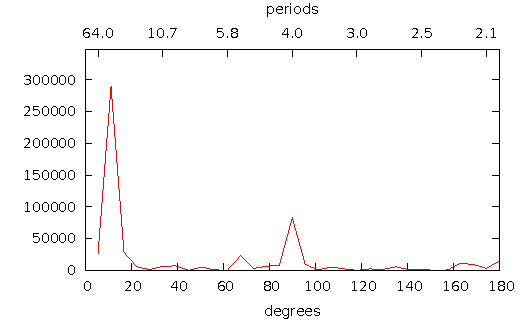
\includegraphics[scale=0.85]{figures/QNCpergm}} \\
  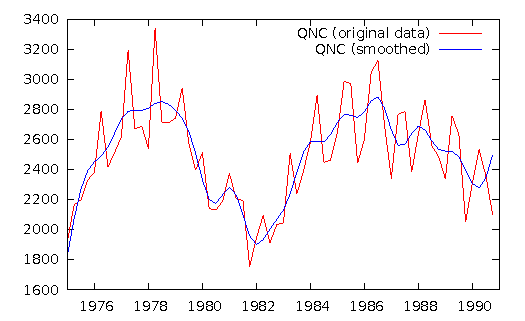
\includegraphics[scale=0.85]{figures/QNCfilt} &
\vbox{\hbox{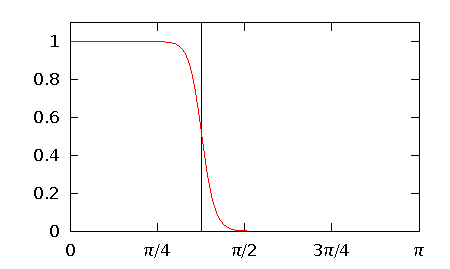
\includegraphics[scale=0.8]{figures/filtergain}}\vskip .3in}
\end{tabular}
\caption{The Butterworth filter applied}
\label{fig:QNCfilt}
\end{figure}

A seasonal pattern is clearly visible in the periodogram, centered at
an angle of 90$^{\circ}$ or 4 periods. If we set $\omega^{\star} =
68^{\circ}$ (or thereabouts) we should be able to excise the
seasonality quite cleanly using $n=8$.  The result is shown in the
lower panel of the Figure, along with the frequency response or gain
plot for the chosen filter. Note the smooth and reasonably steep
drop-off in gain centered on the nominal cutoff of $68^{\circ} \approx
3\pi/8$.

The apparatus that supports this sort of analysis in the \app{gretl}
GUI can be found under the \textsf{Variable} menu in the main window:
the items \textsf{Periodogram} and \textsf{Filter}. In the periodogram
dialog box you have the option of expressing the frequency axis in
degrees, which is helpful when selecting a Butterworth filter; and in
the Butterworth filter dialog you have the option of plotting the
frequency response as well as the smoothed series and/or the residual
or cycle.

%%% Local Variables: 
%%% mode: latex
%%% TeX-master: "gretl-guide"
%%% End: 

\chapter{Univariate time series models}
\label{chap:timeser}

\section{Introduction}
\label{sec:tsintro}

Time series models are discussed in this chapter and the next.  In
this chapter we concentrate on ARIMA models, unit root tests, and
GARCH.  The following chapter deals with cointegration and error
correction.

\section{ARIMA models}
\label{arma-estimation}

\subsection{Representation and syntax}
\label{arma-repr}

The \cmd{arma} command performs estimation of AutoRegressive,
Integrated, Moving Average (ARIMA) models.  These are models that can
be written in the form
\begin{equation}
  \label{eq:plain-0-arma}
  \phi(L) y_t = \theta(L) \epsilon_t
\end{equation}
where $\phi(L)$, and $\theta(L)$ are polynomials in the lag operator,
$L$, defined such that $L^n x_t = x_{t-n}$, and $\epsilon_t$ is a
white noise process. The exact content of $y_t$, of the AR polynomial
$\phi()$, and of the MA polynomial $\theta()$, will be explained in the
following.

\subsection{Mean terms}
\label{sec:arma-nonzeromean}

The process $y_t$ as written in equation (\ref{eq:plain-0-arma}) has,
without further qualifications, mean zero. If the model is to be
applied to real data, it is necessary to include some term to handle
the possibility that $y_t$ has non-zero mean. There are two possible
ways to represent processes with nonzero mean: one is to define $\mu_t$
as the \emph{unconditional} mean of $y_t$, namely the central value of
its marginal distribution. Therefore, the series $\tilde{y}_t = y_t -
\mu_t$ has mean 0, and the model (\ref{eq:plain-0-arma}) applies to
$\tilde{y}_t$. In practice, assuming that $\mu_t$ is a linear function
of some observable variables $x_t$, the model becomes
\begin{equation}
  \label{eq:arma-with-x}
  \phi(L) (y_t - x_t \beta) = \theta(L) \epsilon_t
\end{equation}
This is sometimes known as a ``regression model with ARMA errors'';
its structure may be more apparent if we represent it using two
equations:
\begin{eqnarray*}
  y_t & = & x_t \beta + u_t \\
  \phi(L) u_t & = & \theta(L) \epsilon_t
\end{eqnarray*}

The model just presented is also sometimes known as ``ARMAX'' (ARMA +
eXogenous variables).  It seems to us, however, that this label is
more appropriately applied to a different model: another way to
include a mean term in (\ref{eq:plain-0-arma}) is to base the
representation on the \emph{conditional} mean of $y_t$, that is the
central value of the distribution of $y_t$ \emph{given its own past}.
Assuming, again, that this can be represented as a linear combination
of some observable variables $z_t$, the model would expand to
\begin{equation}
  \label{eq:arma-with-z}
  \phi(L) y_t = z_t \gamma + \theta(L) \epsilon_t
\end{equation}
The formulation (\ref{eq:arma-with-z}) has the advantage that $\gamma$
can be immediately interpreted as the vector of marginal effects of
the $z_t$ variables on the conditional mean of $y_t$.  And by adding
lags of $z_t$ to this specification one can estimate \emph{Transfer
  Function models} (which generalize ARMA by adding the effects of
exogenous variable distributed across time).

\app{Gretl} provides a way to estimate both forms. Models written as
in (\ref{eq:arma-with-x}) are estimated by maximum likelihood; models
written as in (\ref{eq:arma-with-z}) are estimated by conditional
maximum likelihood. (For more on these options see the section on
``Estimation'' below.)  

In the special case when $x_t = z_t = 1$ (that is, the models include
a constant but no exogenous variables) the two specifications discussed
above reduce to
\begin{equation}
  \phi(L) (y_t - \mu) = \theta(L) \epsilon_t
  \label{eq:arma-with-xconst} 
\end{equation}
and
\begin{equation}
  \phi(L) y_t = \alpha + \theta(L) \epsilon_t
  \label{eq:arma-with-zconst}
\end{equation}
respectively.  These formulations are essentially equivalent, but if
they represent one and the same process $\mu$ and $\alpha$ are, fairly
obviously, not numerically identical; rather
\[
\alpha = \left(1 - \phi_1 - \ldots - \phi_p\right) \mu
\]

The \app{gretl} syntax for estimating (\ref{eq:arma-with-xconst}) is simply
\begin{code}
arma p q ; y
\end{code}
The AR and MA lag orders, \texttt{p} and \texttt{q}, can be given either as
numbers or as pre-defined scalars. The parameter $\mu$ can be dropped
if necessary by appending the option \cmd{--nc} (``no constant'') to
the command. If estimation of (\ref{eq:arma-with-zconst}) is needed,
the switch \option{conditional} must be appended to the command, as
in 
\begin{code}
arma p q ; y --conditional
\end{code}

Generalizing this principle to the estimation of
(\ref{eq:arma-with-x}) or (\ref{eq:arma-with-z}), you get that
\begin{code}
arma p q ; y const x1 x2
\end{code}
would estimate the following model:
\[
  y_t - x_t \beta = \phi_1 \left(y_{t-1} - x_{t-1} \beta \right) + \ldots + 
   \phi_p \left( y_{t-p} - x_{t-p} \beta \right) + 
  \epsilon_t + \theta_1 \epsilon_{t-1} + \ldots + \theta_q \epsilon_{t-q}
\]
where in this instance $x_t \beta = \beta_0 + x_{t,1} \beta_1 +
x_{t,2} \beta_2$. Appending the \option{conditional} switch, as in 
\begin{code}
arma p q ; y const x1 x2 --conditional
\end{code}
would estimate the following model:
\[
  y_t = x_t \gamma + \phi_1 y_{t-1} + \ldots +  \phi_p y_{t-p} + 
  \epsilon_t + \theta_1 \epsilon_{t-1} + \ldots + \theta_q \epsilon_{t-q}
\]

Ideally, the issue broached above could be made moot by writing a more
general specification that nests the alternatives; that is
\begin{equation}
 \label{armax-general}
  \phi(L) \left(y_t - x_t \beta\right) = z_t \gamma  + \theta(L) \epsilon_t ;
\end{equation}
we would like to generalize the \cmd{arma} command so that
the user could specify, for any estimation method, whether certain
exogenous variables should be treated as $x_t$s or $z_t$s, but we're
not yet at that point (and neither are most other software packages).


\subsection{Seasonal models}

A more flexible lag structure is desirable when analyzing time series
that display strong seasonal patterns. Model (\ref{eq:plain-0-arma})
can be expanded to
\begin{equation}
  \label{eq:seasonal-arma}
  \phi(L) \Phi(L^s) y_t = \theta(L) \Theta(L^s) \epsilon_t .
\end{equation}
For such cases, a fuller form of the syntax is available, namely,
\begin{code}
arma p q ; P Q ; y
\end{code}
where \texttt{p} and \texttt{q} represent the non-seasonal AR and MA
orders, and \texttt{P} and \texttt{Q} the seasonal orders.  For
example,
\begin{code}
arma 1 1 ; 1 1 ; y
\end{code}
would be used to estimate the following model:
\[
  (1 -\phi L)(1 -\Phi L^s) (y_t - \mu) = (1 + \theta L)(1 + \Theta L^s) \epsilon_t
\]
If $y_t$ is a quarterly series (and therefore $s=4$), the above
equation can be written more explicitly as
\[
y_t - \mu = \phi (y_{t-1} - \mu) + \Phi (y_{t-4} - \mu) - (\phi
  \cdot \Phi) (y_{t-5} - \mu) + \epsilon_t + \theta \epsilon_{t-1} + \Theta
  \epsilon_{t-4} + (\theta \cdot \Theta) \epsilon_{t-5}
\]
Such a model is known as a ``multiplicative seasonal ARMA model''.


\subsection{Gaps in the lag structure}

The standard way to specify an ARMA model in \app{gretl} is via the AR
and MA orders, $p$ and $q$ respectively.  In this case all lags from 1
to the given order are included.  In some cases one may wish to
include only certain specific AR and/or MA lags.  This can be done in
either of two ways.
%
\begin{itemize}
\item One can construct a matrix containing the desired lags (positive
  integer values) and supply the name of this matrix in place of $p$
  or $q$.
\item One can give a space-separated list of lags, enclosed in braces,
  in place of $p$ or $q$.
\end{itemize}
%
The following code illustrates these options:
%
\begin{code}
matrix pvec = {1, 4}
arma pvec 1 ; y
arma {1 4} 1 ; y
\end{code}
%
Both forms above specify an ARMA model in which AR lags 1 and 4 are
used (but not 2 and 3). 

This facility is available only for the non-seasonal component of
the ARMA specification.

\subsection{Differencing and ARIMA}

The above discussion presupposes that the time series $y_t$ has
already been subjected to all the transformations deemed necessary for
ensuring stationarity (see also section \ref{sec:uroot}). Differencing
is the most common of these transformations, and \app{gretl} provides
a mechanism to include this step into the \cmd{arma} command: the
syntax
\begin{code}
arma p d q ; y 
\end{code}
would estimate an ARMA$(p,q)$ model on $\Delta^d y_t$. It is
functionally equivalent to 
\begin{code}
series tmp = y
loop i=1..d
  tmp = diff(tmp)
endloop
arma p q ; tmp 
\end{code}
except with regard to forecasting after estimation (see below).

When the series $y_t$ is differenced before performing the analysis
the model is known as ARIMA (``I'' for Integrated); for this reason,
\app{gretl} provides the \cmd{arima} command as an alias for
\cmd{arma}.

Seasonal differencing is handled similarly, with the syntax
\begin{code}
arma p d q ; P D Q ; y 
\end{code}
where \texttt{D} is the order for seasonal differencing.  Thus, the
command
\begin{code}
arma 1 0 0 ; 1 1 1 ; y 
\end{code}
would produce the same parameter estimates as
\begin{code}
genr dsy = sdiff(y)
arma 1 0 ; 1 1 ; dsy 
\end{code}
where we use the \texttt{sdiff} function to create a seasonal
difference (e.g.\ for quarterly data, $y_t - y_{t-4}$).

In specifying an ARIMA model with exogenous regressors we face a
choice which relates back to the discussion of the variant models
(\ref{eq:arma-with-x}) and (\ref{eq:arma-with-z}) above.  If we choose
model (\ref{eq:arma-with-x}), the ``regression model with ARMA
errors'', how should this be extended to the case of ARIMA?  The issue
is whether or not the differencing that is applied to the dependent
variable should also be applied to the regressors.  Consider the
simplest case, ARIMA with non-seasonal differencing of order 1. We may
estimate either
\begin{equation}
  \label{eq:arima-with-x}
  \phi(L) (1-L) (y_t - X_t\beta) = \theta(L) \epsilon_t
\end{equation}
or
\begin{equation}
  \label{eq:arima-with-z}
  \phi(L) \left((1-L) y_t - X_t\beta\right) = \theta(L) \epsilon_t
\end{equation}
%
The first of these formulations can be described as a regression model
with ARIMA errors, while the second preserves the levels of the $X$
variables.  As of \app{gretl} version 1.8.6, the default model is
(\ref{eq:arima-with-x}), in which differencing is applied to both
$y_t$ and $X_t$.  However, when using the default estimation method
(native exact ML, see below), the option \option{y-diff-only} may be
given, in which case \app{gretl} estimates
(\ref{eq:arima-with-z}).\footnote{Prior to \app{gretl} 1.8.6, the
  default model was (\ref{eq:arima-with-z}).  We changed this for the
  sake of consistency with other software.}


\subsection{Estimation}
\label{arma-est}

The default estimation method for ARMA models is exact maximum
likelihood estimation (under the assumption that the error term is
normally distributed), using the Kalman filter in conjunction with the
BFGS maximization algorithm.  The gradient of the log-likelihood with
respect to the parameter estimates is approximated numerically.  This
method produces results that are directly comparable with many other
software packages.  The constant, and any exogenous variables, are
treated as in equation (\ref{eq:arma-with-x}).  The covariance matrix
for the parameters is computed using a numerical approximation to the
Hessian at convergence.

The alternative method, invoked with the \option{conditional} switch,
is conditional maximum likelihood (CML), also known as ``conditional
sum of squares'' \citep[see][p.\ 132]{hamilton94}.  This method was
exemplified in the script~\ref{jack-arma}, and only a brief
description will be given here.  Given a sample of size $T$, the CML
method minimizes the sum of squared one-step-ahead prediction errors
generated by the model for the observations $t_0, \ldots, T$.  The
starting point $t_0$ depends on the orders of the AR polynomials in
the model.  The numerical maximization method used is BHHH, and the
covariance matrix is computed using a Gauss--Newton regression.

The CML method is nearly equivalent to maximum likelihood under the
hypothesis of normality; the difference is that the first $(t_0 - 1)$
observations are considered fixed and only enter the likelihood
function as conditioning variables. As a consequence, the two methods
are asymptotically equivalent under standard conditions --- except for
the fact, discussed above, that our CML implementation treats the
constant and exogenous variables as per equation (\ref{eq:arma-with-z}).

The two methods can be compared as in the following example
\begin{code}
open data10-1
arma 1 1 ; r
arma 1 1 ; r --conditional
\end{code}
which produces the estimates shown in Table~\ref{tab:ml-cml}.  As you
can see, the estimates of $\phi$ and $\theta$ are quite similar.  The
reported constants differ widely, as expected --- see the discussion
following equations (\ref{eq:arma-with-xconst}) and
(\ref{eq:arma-with-zconst}).  However, dividing the CML constant by
$1-\phi$ we get 7.38, which is not far from the ML estimate of 6.93.

\begin{table}[htbp]
\caption{ML and CML estimates}
\label{tab:ml-cml}
\begin{center}
  \begin{tabular}{crrrr}
    \hline
    Parameter & \multicolumn{2}{c}{ML} &
    \multicolumn{2}{c}{CML} \\
    \hline 
    $\mu$ & 6.93042 & (0.923882) & 1.07322 & (0.488661) \\
    $\phi$ & 0.855360 & (0.0511842) & 0.852772 & (0.0450252) \\
    $\theta$ & 0.588056 & (0.0986096) & 0.591838 & (0.0456662) \\
    \hline
  \end{tabular}
\end{center}
\end{table}

\subsection{Convergence and initialization}

The numerical methods used to maximize the likelihood for ARMA models
are not guaranteed to converge.  Whether or not convergence is
achieved, and whether or not the true maximum of the likelihood
function is attained, may depend on the starting values for the
parameters.  \app{Gretl} employs one of the following two
initialization mechanisms, depending on the specification of the model
and the estimation method chosen.

\begin{enumerate}
\item Estimate a pure AR model by Least Squares (nonlinear least
  squares if the model requires it, otherwise OLS).  Set the AR
  parameter values based on this regression and set the MA
  parameters to a small positive value (0.0001).
\item The Hannan--Rissanen method: First estimate an autoregressive
  model by OLS and save the residuals.  Then in a second OLS pass add
  appropriate lags of the first-round residuals to the model, to
  obtain estimates of the MA parameters.
\end{enumerate}

To see the details of the ARMA estimation procedure, add the
\option{verbose} option to the command.  This prints a notice of the
initialization method used, as well as the parameter values and
log-likelihood at each iteration.

Besides the built-in initialization mechanisms, the user has the
option of specifying a set of starting values manually.  This is done
via the \cmd{set} command: the first argument should be the keyword
\texttt{initvals} and the second should be the name of a pre-specified
matrix containing starting values.  For example
\begin{code}
matrix start = { 0, 0.85, 0.34 }
set initvals start
arma 1 1 ; y
\end{code}
The specified matrix should have just as many parameters as the model:
in the example above there are three parameters, since the model
implicitly includes a constant.  The constant, if present, is always
given first; otherwise the order in which the parameters are
expected is the same as the order of specification in the \cmd{arma}
or \cmd{arima} command.  In the example the constant is set to zero,
$\phi_1$ to 0.85, and $\theta_1$ to 0.34.

You can get \app{gretl} to revert to automatic initialization via
the command \cmd{set initvals auto}.

Two variants of the BFGS algorithm are available in \app{gretl}.  In
general we recommend the default variant, which is based on an
implementation by \cite{nash90}, but for some problems the
alternative, limited-memory version (L-BFGS-B, see
\citealp{byrd-etal95}) may increase the chances of convergence on the
ML solution.  This can be selected via the \option{lbfgs} option to
the \texttt{arma} command.

\subsection{Estimation via X-12-ARIMA}

As an alternative to estimating ARMA models using ``native'' code,
\app{gretl} offers the option of using the external program
\app{X-12-ARIMA}.  This is the seasonal adjustment software produced
and maintained by the U.S. Census Bureau; it is used for all official
seasonal adjustments at the Bureau.

\app{Gretl} includes a module which interfaces with \app{X-12-ARIMA}:
it translates \cmd{arma} commands using the syntax outlined above into
a form recognized by \app{X-12-ARIMA}, executes the program, and
retrieves the results for viewing and further analysis within
\app{gretl}.  To use this facility you have to install
\app{X-12-ARIMA} separately.  Packages for both MS Windows and
GNU/Linux are available from the \app{gretl} website,
\url{http://gretl.sourceforge.net/}.

To invoke \app{X-12-ARIMA} as the estimation engine, append the flag
\verb|--x-12-arima|, as in
\begin{code}
arma p q ; y --x-12-arima
\end{code}
As with native estimation, the default is to use exact ML but there is
the option of using conditional ML with the \option{conditional} flag.
However, please note that when \app{X-12-ARIMA} is used in conditional
ML mode, the comments above regarding the variant treatments of the
mean of the process $y_t$ \textit{do not apply}.  That is, when you
use \app{X-12-ARIMA} the model that is estimated is
(\ref{eq:arma-with-x}), regardless of whether estimation is by exact
ML or conditional ML.  In addition, the treatment of exogenous
regressors in the context of ARIMA differencing is always that shown
in equation (\ref{eq:arima-with-x}).


\subsection{Forecasting}
\label{arma-fcast}

ARMA models are often used for forecasting purposes.  The
autoregressive component, in particular, offers the possibility of
forecasting a process ``out of sample'' over a substantial time
horizon.

\app{Gretl} supports forecasting on the basis of ARMA models using the
method set out by \cite{box-jenkins76}.\footnote{See in particular
  their ``Program 4'' on p.\ 505ff.}  The Box and Jenkins algorithm
produces a set of integrated AR coefficients which take into account
any differencing of the dependent variable (seasonal and/or
non-seasonal) in the ARIMA context, thus making it possible to
generate a forecast for the level of the original variable.  By
contrast, if you first difference a series manually and then apply
ARMA to the differenced series, forecasts will be for the differenced
series, not the level.  This point is illustrated
in Example~\ref{arima-fcast-script}.  The parameter estimates are identical
for the two models.  The forecasts differ but are mutually consistent:
the variable \texttt{fcdiff} emulates the ARMA forecast (static,
one step ahead within the sample range, and dynamic out of sample).

\begin{script}[htbp]
  \caption{ARIMA forecasting}
  \label{arima-fcast-script}
\begin{scode}
open greene18_2.gdt
# log of quarterly U.S. nominal GNP, 1950:1 to 1983:4
genr y = log(Y)
# and its first difference
genr dy = diff(y)
# reserve 2 years for out-of-sample forecast
smpl ; 1981:4
# Estimate using ARIMA
arima 1 1 1 ; y 
# forecast over full period
smpl --full
fcast fc1
# Return to sub-sample and run ARMA on the first difference of y
smpl ; 1981:4
arma 1 1 ; dy
smpl --full
fcast fc2
genr fcdiff = (t<=1982:1)? (fc1 - y(-1)) : (fc1 - fc1(-1))
# compare the forecasts over the later period
smpl 1981:1 1983:4
print y fc1 fc2 fcdiff --byobs
\end{scode}
The output from the last command is:
%
\begin{code}
                  y          fc1          fc2       fcdiff
1981:1      7.964086     7.940930      0.02668      0.02668
1981:2      7.978654     7.997576      0.03349      0.03349
1981:3      8.009463     7.997503      0.01885      0.01885
1981:4      8.015625     8.033695      0.02423      0.02423
1982:1      8.014997     8.029698      0.01407      0.01407
1982:2      8.026562     8.046037      0.01634      0.01634
1982:3      8.032717     8.063636      0.01760      0.01760
1982:4      8.042249     8.081935      0.01830      0.01830
1983:1      8.062685     8.100623      0.01869      0.01869
1983:2      8.091627     8.119528      0.01891      0.01891
1983:3      8.115700     8.138554      0.01903      0.01903
1983:4      8.140811     8.157646      0.01909      0.01909
\end{code}
\end{script}


\section{Unit root tests}
\label{sec:uroot}

\subsection{The ADF test}
\label{sec:ADFtest}

The Augmented Dickey--Fuller (ADF) test is, as implemented in
\app{gretl}, the $t$-statistic on $\varphi$ in the following regression:
\begin{equation}
  \label{eq:ADFtest}
  \Delta y_t = \mu_t + \varphi y_{t-1} + \sum_{i=1}^p \gamma_i \Delta
  y_{t-i} + \epsilon_t .
\end{equation}

This test statistic is probably the best-known and most widely used
unit root test. It is a one-sided test whose null hypothesis is
$\varphi = 0$ versus the alternative $\varphi < 0$ (and hence large
negative values of the test statistic lead to the rejection of the
null).  Under the null, $y_t$ must be differenced at least once to
achieve stationarity; under the alternative, $y_t$ is already
stationary and no differencing is required.

One peculiar aspect of this test is that its limit distribution is
non-standard under the null hypothesis: moreover, the shape of the
distribution, and consequently the critical values for the test,
depends on the form of the $\mu_t$ term.  A full analysis of the
various cases is inappropriate here: \cite{hamilton94} contains an
excellent discussion, but any recent time series textbook covers
this topic. Suffice it to say that \app{gretl} allows the user to
choose the specification for $\mu_t$ among four different
alternatives:

\begin{center}
  \begin{tabular}{cc}
    \hline
    $\mu_t$ & command option \\
    \hline
    0 & \option{nc} \\
    $\mu_0$ &  \option{c} \\
    $\mu_0 + \mu_1 t$ &  \option{ct} \\
    $\mu_0 + \mu_1 t + \mu_1 t^2$ &  \option{ctt} \\
    \hline
  \end{tabular}
\end{center}

These option flags are not mutually exclusive; when they are used
together the statistic will be reported separately for each selected
case.  By default, \app{gretl} uses the combination \verb|--c --ct|.
For each case, approximate p-values are calculated by means of the
algorithm developed in \cite{mackinnon96}.

The \app{gretl} command used to perform the test is \cmd{adf}; for example
\begin{code}
adf 4 x1
\end{code}
would compute the test statistic as the $t$-statistic for $\varphi$ in
equation \ref{eq:ADFtest} with $p=4$ in the two cases $\mu_t = \mu_0$
and $\mu_t = \mu_0 + \mu_1 t$.

The number of lags ($p$ in equation \ref{eq:ADFtest}) should be chosen
as to ensure that (\ref{eq:ADFtest}) is a parametrization flexible
enough to represent adequately the short-run persistence of $\Delta
y_t$. Setting $p$ too low results in size distortions in the test,
whereas setting $p$ too high leads to low power. As a convenience
to the user, the parameter $p$ can be automatically determined.
Setting $p$ to a negative number triggers a sequential procedure that
starts with $p$ lags and decrements $p$ until the $t$-statistic for
the parameter $\gamma_p$ exceeds 1.645 in absolute value.

\subsection{The ADF-GLS test}
\label{sec:ADF-GLS}

\citet*{ERS96} proposed a variant of the ADF test which involves an
alternative method of handling the parameters pertaining to the
deterministic term $\mu_t$: these are estimated first via Generalized
Least Squares, and in a second stage an ADF regression is performed
using the GLS residuals. This variant offers greater power than the
regular ADF test for the cases $\mu_t = \mu_0$ and $\mu_t = \mu_0 +
\mu_1 t$. 

The ADF-GLS test is available in \app{gretl} via the \verb|--gls|
option to the \texttt{adf} command. When this option is selected the
\verb|--nc| and \verb|--ctt| options become unavailable, and only one
case can be selected at a time; by default the constant-only model is
used but a trend can be added using the \verb|--ct| flag.  When a
trend is present in this test MacKinnon-type p-values are not
available; instead we show critical values from Table 1 in
\cite{ERS96}.


\subsection{The KPSS test}
\label{sec:KPSStest}

The KPSS test \citep*{KPSS92} is a unit root test in which the null
hypothesis is opposite to that in the ADF test: under the null, the
series in question is stationary; the alternative is that the series
is $I(1)$.

The basic intuition behind this test statistic is very simple: if
$y_t$ can be written as $y_t = \mu + u_t$, where $u_t$ is some
zero-mean stationary process, then not only does the sample average of
the $y_t$s provide a consistent estimator of $\mu$, but the long-run
variance of $u_t$ is a well-defined, finite number. Neither of these
properties hold under the alternative.

The test itself is based on the following statistic:
\begin{equation}
  \label{eq:KPSStest}
  \eta = \frac{\sum_{i=1}^T S_t^2 }{ T^2 \bar{\sigma}^2 }
\end{equation}
where $S_t = \sum_{s=1}^t e_s$ and $\bar{\sigma}^2$ is an estimate of
the long-run variance of $e_t = (y_t - \bar{y})$. Under the null, this
statistic has a well-defined (nonstandard) asymptotic distribution,
which is free of nuisance parameters and has been tabulated by
simulation. Under the alternative, the statistic diverges.

As a consequence, it is possible to construct a one-sided test based
on $\eta$, where $H_0$ is rejected if $\eta$ is bigger than the
appropriate critical value; \app{gretl} provides the 90, 95 and 99
percent quantiles. The critical values are computed via the method
presented by \cite{sephton95}, which offers greater accuracy than the
values tabulated in \cite{KPSS92}.

Usage example:
\begin{code}
kpss m y
\end{code}
where \verb|m| is an integer representing the bandwidth or window
size used in the formula for estimating the long run variance:
\[
  \bar{\sigma}^2 = \sum_{i=-m}^m \left( 1 - \frac{|i|}{m+1} \right) \hat{\gamma}_i
\]
The $\hat{\gamma}_i$ terms denote the empirical autocovariances of
$e_t$ from order $-m$ through $m$.  For this estimator to be
consistent, $m$ must be large enough to accommodate the short-run
persistence of $e_t$, but not too large compared to the sample size
$T$.  If the supplied \verb|m| is non-positive a default value is
computed, namely the integer part of $4 \left( \frac{T}{100}
\right)^{1/4}$.

The above concept can be generalized to the case where $y_t$ is
thought to be stationary around a deterministic trend. In this case,
formula (\ref{eq:KPSStest}) remains unchanged, but the series $e_t$ is
defined as the residuals from an OLS regression of $y_t$ on a constant
and a linear trend. This second form of the test is obtained by
appending the \option{trend} option to the \cmd{kpss} command:
\begin{code}
kpss n y --trend
\end{code}
Note that in this case the asymptotic distribution of the test is
different and the critical values reported by \app{gretl} differ
accordingly.


\subsection{Panel unit root tests}
\label{sec:panel-uroot}

The most commonly used unit root tests for panel data involve a
generalization of the ADF procedure, in which the joint null
hypothesis is that a given times series is non-stationary for all
individuals in the panel.

In this context the ADF regression (\ref{eq:ADFtest}) can be rewritten
as

\begin{equation}
  \label{eq:panelADF}
  \Delta y_{it} = \mu_{it} + \varphi_i y_{i,t-1} + \sum_{j=1}^{p_i} \gamma_{ij} \Delta
  y_{i,t-j} + \epsilon_{it}
\end{equation}

The model (\ref{eq:panelADF}) allows for maximal heterogeneity across
the individuals in the panel: the parameters of the deterministic
term, the autoregressive coefficient $\varphi$, and the lag order $p$
are all specific to the individual, indexed by $i$.

One possible modification of this model is to impose the assumption
that $\varphi_i = \varphi$ for all $i$; that is, the individual time
series share a common autoregressive root (although they may differ in
respect of other statistical properties). The choice of whether or not
to impose this assumption has an important bearing on the hypotheses
under test. Under model (\ref{eq:panelADF}) the joint null is
$\varphi_i = 0$ for all $i$, meaning that all the individual time
series are non-stationary, and the alternative (simply the negation of
the null) is that \emph{at least one} individual time series is
stationary.  When a common $\varphi$ is assumed, the null is that
$\varphi = 0$ and the alternative is that $\varphi < 0$. The null
still says that all the individual series are non-stationary, but the
alternative now says that they are \emph{all} stationary.  The choice
of model should take this point into account, as well as the gain in
power from forming a pooled estimate of $\varphi$ and, of course, the
plausibility of assuming a common AR(1) coefficient.\footnote{If the
  assumption of a common $\varphi$ seems excessively restrictive, bear
  in mind that we routinely assume common slope coefficients when
  estimating panel models, even if this is unlikely to be literally
  true.}

In \app{gretl}, the formulation (\ref{eq:panelADF}) is used
automatically when the \texttt{adf} command is used on panel data. The
joint test statistic is formed using the method of \citet*{IPS03}. In
this context the behavior of \texttt{adf} differs from regular
time-series data: only one case of the deterministic term is handled
per invocation of the command; the default is that $\mu_{it}$ includes
just a constant but the \verb|--nc| and \verb|--ct| flags can be used
to suppress the constant or to include a trend, respectively; and the
quadratic trend option \verb|--ctt| is not available.

The alternative that imposes a common value of $\varphi$ is
implemented via the \texttt{levinlin} command. The test statistic is
computed as per \citet*{LLC2002}.  As with the \texttt{adf} command, the
first argument is the lag order and the second is the name of the
series to test; and the default case for the deterministic component
is a constant only. The options \verb|--nc| and \verb|--ct| have the
same effect as with \texttt{adf}. One refinement is that the lag order
may be given in either of two forms: if a scalar is given, this is
taken to represent a common value of $p$ for all individuals, but you
may instead provide a vector holding a set of $p_i$ values, hence
allowing the order of autocorrelation of the series to differ by
individual. So, for example, given
\begin{code}
levinlin 2 y
levinlin {2,2,3,3,4,4} y
\end{code}
the first command runs a joint ADF test with a common lag order of 2,
while the second (which assumes a panel with six individuals) allows
for differing short-run dynamics. The first argument to
\texttt{levinlin} can be given as a set of comma-separated integers
enclosed in braces, as shown above, or as the name of an appropriately
dimensioned pre-defined matrix (see chapter~\ref{chap:matrices}).

Besides variants of the ADF test, the KPSS test also can be used with
panel data via the \texttt{kpss} command. In this case the test (of
the null hypothesis that the given time series is \emph{stationary}
for all individuals) is implemented using the method of
\cite{choi01}. This is an application of \emph{meta-analysis}, the
statistical technique whereby an overall or composite p-value for the
test of a given null hypothesis can be computed from the p-values of a
set of separate tests. Unfortunately, in the case of the KPSS test we
are limited by the unavailability of precise p-values, although if an
individual test statistic falls between the 10 percent and 1 percent
critical values we are able to interpolate with a fair degree of
confidence. This gives rise to four cases.

\begin{enumerate}
\item All the individual KPSS test statistics fall between the 10
  percent and 1 percent critical values: the Choi method gives us
  a plausible composite p-value.
\item Some of the KPSS test statistics exceed the 1 percent value and
  none fall short of the 10 percent value: we can give an upper bound
  for the composite p-value by setting the unknown p-values to 0.01.
\item Some of the KPSS test statistics fall short of the 10 percent
  critical value but none exceed the 1 percent value: we can give a
  lower bound to the composite p-value by setting the unknown p-values
  to 0.10.
\item None of the above conditions are satisfied: the Choi method
  fails to produce any result for the composite KPSS test.
\end{enumerate}


\section{Cointegration tests}
\label{sec:coint-test}

The generally recommended test for cointegration is the Johansen test,
which is discussed in detail in chapter~\ref{chap:vecm}. In this
context we offer a few remarks on the cointegration test of
\cite{engle-granger87}, which builds on the ADF test discussed above
(section~\ref{sec:ADFtest}).

For the Engle--Granger test, the procedure is:
\begin{enumerate}
\item Test each series for a unit root using an ADF test.
\item Run a ``cointegrating regression'' via OLS. For this we select
  one of the potentially cointegrated variables as dependent, and
  include the other potentially cointegrated variables as regressors.
\item Perform an ADF test on the residuals from the cointegrating
  regression.
\end{enumerate}

The idea is that cointegration is supported if (a) the null of
non-stationarity is \emph{not} rejected for each of the series
individually, in step 1, while (b) the null \emph{is} rejected for the
residuals at step 3. That is, each of the individual series is $I(1)$
but some linear combination of the series is $I(0)$.  

This test is implemented in \app{gretl} by the \texttt{coint} command,
which requires an integer lag order (for the ADF tests) followed by a
list of variables to be tested, the first of which will be taken as
dependent in the cointegrating regression. Please see the online help
for \texttt{coint}, or the \textit{Gretl Command Reference}, for
further details.


\section{ARCH and GARCH}
\label{sec:arch-garch}

Heteroskedasticity means a non-constant variance of the error term in
a regression model.  Autoregressive Conditional Heteroskedasticity
(ARCH) is a phenomenon specific to time series models, whereby the
variance of the error displays autoregressive behavior; for instance,
the time series exhibits successive periods where the error variance
is relatively large, and successive periods where it is relatively
small.  This sort of behavior is reckoned to be quite common in asset
markets: an unsettling piece of news can lead to a period of increased
volatility in the market.

An ARCH error process of order $q$ can be represented as
\[
u_t = \sigma_t \varepsilon_t; \qquad
\sigma^2_t \equiv {\rm E}(u^2_t|\Omega_{t-1}) = 
\alpha_0 + \sum_{i=1}^q \alpha_i u^2_{t-i}
\]
where the $\varepsilon_t$s are independently and identically
distributed (iid) with mean zero and variance 1, and where $\sigma_t$
is taken to be the positive square root of $\sigma^2_t$.
$\Omega_{t-1}$ denotes the information set as of time $t-1$ and
$\sigma^2_t$ is the conditional variance: that is, the
variance conditional on information dated $t-1$ and earlier.

It is important to notice the difference between ARCH and an ordinary
autoregressive error process.  The simplest (first-order) case of the
latter can be written as
\[
u_t = \rho u_{t-1} + \varepsilon_t; \qquad -1 < \rho < 1
\]
where the $\varepsilon_t$s are independently and identically
distributed with mean zero and variance $\sigma^2$.  With an
AR(1) error, if $\rho$ is positive then a positive value of $u_t$ will
tend to be followed, with probability greater than 0.5, by a positive
$u_{t+1}$.  With an ARCH error process, a disturbance $u_t$ of large
absolute value will tend to be followed by further large absolute
values, but with no presumption that the successive values will be of
the same sign.  ARCH in asset prices is a ``stylized fact'' and is
consistent with market efficiency; on the other hand autoregressive
behavior of asset prices would violate market efficiency.

One can test for ARCH of order $q$ in the following
way:
\begin{enumerate}
\item Estimate the model of interest via OLS and save the squared
  residuals, $\hat{u}^2_t$.
\item Perform an auxiliary regression in which the current squared
  residual is regressed on a constant and $q$ lags of itself.
\item Find the $TR^2$ value (sample size times unadjusted $R^2$) for
  the auxiliary regression.
\item Refer the $TR^2$ value to the $\chi^2$ distribution with $q$
  degrees of freedom, and if the p-value is ``small enough'' reject
  the null hypothesis of homoskedasticity in favor of the alternative
  of ARCH($q$).
\end{enumerate}

This test is implemented in \app{gretl} via the \cmd{modtest} command
with the \option{arch} option, which must follow estimation of a
time-series model by OLS (either a single-equation model or a
VAR). For example,
%
\begin{code}
ols y 0 x
modtest 4 --arch
\end{code}

This example specifies an ARCH order of $q=4$; if the order argument
is omitted, $q$ is set equal to the periodicity of the data.  In the
graphical interface, the ARCH test is accessible from the ``Tests''
menu in the model window (again, for single-equation OLS or VARs).

\subsection{GARCH}
\label{subsec:garch}

The simple ARCH($q$) process is useful for introducing the general
concept of conditional heteroskedasticity in time series, but it has
been found to be insufficient in empirical work.  The dynamics of the
error variance permitted by ARCH($q$) are not rich enough to represent 
the patterns found in financial data.  The generalized ARCH or GARCH
model is now more widely used.  

The representation of the variance of a process in the GARCH model is
somewhat (but not exactly) analogous to the ARMA representation of the
level of a time series.  The variance at time $t$ is allowed
to depend on both past values of the variance and past values of the
realized squared disturbance, as shown in the following system
of equations:
\begin{eqnarray}
  \label{eq:garch-meaneq}
  y_t &  = & X_t \beta + u_t \\
  \label{eq:garch-epseq}
  u_t &  = & \sigma_t \varepsilon_t \\
  \label{eq:garch-vareq}
  \sigma^2_t & = & \alpha_0 + \sum_{i=1}^q \alpha_i u^2_{t-i} +
	  \sum_{j=1}^p \delta_j \sigma^2_{t-j}
\end{eqnarray}
As above, $\varepsilon_t$ is an iid sequence with unit variance.
$X_t$ is a matrix of regressors (or in the simplest case,
just a vector of 1s allowing for a non-zero mean of $y_t$).  Note that
if $p=0$, GARCH collapses to ARCH($q$): the generalization is embodied
in the $\delta_j$ terms that multiply previous values of the error
variance.

In principle the underlying innovation, $\varepsilon_t$, could follow
any suitable probability distribution, and besides the obvious
candidate of the normal or Gaussian distribution the Student's $t$
distribution has been used in this context.  Currently \app{gretl}
only handles the case where $\varepsilon_t$ is assumed to be Gaussian.
However, when the \option{robust} option to the \cmd{garch} command is
given, the estimator \app{gretl} uses for the covariance matrix can be
considered Quasi-Maximum Likelihood even with non-normal disturbances.
See below for more on the options regarding the GARCH covariance
matrix.

Example:
\begin{code}
garch p q ; y const x
\end{code}
where \verb|p| $\ge 0$ and \verb|q| $>0$ denote the respective lag
orders as shown in equation (\ref{eq:garch-vareq}).  These values
can be supplied in numerical form or as the names of pre-defined
scalar variables.

\subsection{GARCH estimation}
\label{subsec:garch-est}

Estimation of the parameters of a GARCH model is by no means a
straightforward task.  (Consider equation~\ref{eq:garch-vareq}: the
conditional variance at any point in time, $\sigma^2_t$, depends on
the conditional variance in earlier periods, but $\sigma^2_t$ is not
observed, and must be inferred by some sort of Maximum Likelihood
procedure.)  By default \app{gretl} uses native code that employs the
BFGS maximizer; you also have the option (activated by the
\verb|--fcp| command-line switch) of using the method proposed by
\cite{fiorentini96},\footnote{The algorithm is based on Fortran code
  deposited in the archive of the \textit{Journal of Applied
    Econometrics} by the authors, and is used by kind permission of
  Professor Fiorentini.} which was adopted as a benchmark in the study
of GARCH results by \cite{mccullough98}.  It employs analytical first
and second derivatives of the log-likelihood, and uses a
mixed-gradient algorithm, exploiting the information matrix in the
early iterations and then switching to the Hessian in the neighborhood
of the maximum likelihood.  (This progress can be observed if you
append the \option{verbose} option to \app{gretl}'s \cmd{garch}
command.)

Several options are available for computing the covariance matrix of
the parameter estimates in connection with the \cmd{garch} command.
At a first level, one can choose between a ``standard'' and a
``robust'' estimator.  By default, the Hessian is used unless the
\option{robust} option is given, in which case the QML estimator is
used.  A finer choice is available via the \cmd{set} command, as
shown in Table~\ref{tab:garch-vcv}.

\begin{table}[htbp]
\caption{Options for the GARCH covariance matrix}
\label{tab:garch-vcv}
\begin{center}
\begin{tabular}{ll}
\multicolumn{1}{c}{\textit{command}} &
\multicolumn{1}{c}{\textit{effect}} \\ [4pt]
\texttt{set garch\_vcv hessian} & Use the Hessian \\
\texttt{set garch\_vcv im} & Use the Information Matrix \\
\texttt{set garch\_vcv op} & Use the Outer Product of the Gradient \\
\texttt{set garch\_vcv qml} & QML estimator \\
\texttt{set garch\_vcv bw} & Bollerslev--Wooldridge ``sandwich'' estimator
\end{tabular}
\end{center}
\end{table}

It is not uncommon, when one estimates a GARCH model for an arbitrary
time series, to find that the iterative calculation of the estimates
fails to converge.  For the GARCH model to make sense, there are
strong restrictions on the admissible parameter values, and it is not
always the case that there exists a set of values inside the
admissible parameter space for which the likelihood is maximized.  

The restrictions in question can be explained by reference to the
simplest (and much the most common) instance of the GARCH model, where
$p = q = 1$.  In the GARCH(1, 1) model the conditional variance is
\begin{equation}
\label{eq:condvar}
\sigma^2_t = \alpha_0 + \alpha_1 u^2_{t-1} + \delta_1 \sigma^2_{t-1}
\end{equation}
Taking the unconditional expectation of (\ref{eq:condvar}) we get
\[
\sigma^2 = \alpha_0 + \alpha_1 \sigma^2 + \delta_1 \sigma^2
\]
so that
\[
\sigma^2 = \frac{\alpha_0}{1 - \alpha_1 - \delta_1}
\]
For this unconditional variance to exist, we require that $\alpha_1 +
\delta_1 < 1$, and for it to be positive we require that $\alpha_0 > 0$.

A common reason for non-convergence of GARCH estimates (that is, a
common reason for the non-existence of $\alpha_i$ and $\delta_i$ values
that satisfy the above requirements and at the same time maximize the
likelihood of the data) is misspecification of the model.  It is
important to realize that GARCH, in itself, allows \textit{only} for
time-varying volatility in the data.  If the \textit{mean} of the
series in question is not constant, or if the error process is not
only heteroskedastic but also autoregressive, it is necessary to take
this into account when formulating an appropriate model.  For example,
it may be necessary to take the first difference of the variable in
question and/or to add suitable regressors, $X_t$, as in
(\ref{eq:garch-meaneq}).

%%% Local Variables: 
%%% mode: latex
%%% TeX-master: "gretl-guide"
%%% End: 


\chapter{Vector Autoregressions}
\label{chap:var}

Gretl provides a standard set of procedures for dealing with the
multivariate time-series models known as VARs (\emph{Vector
  AutoRegression}). More general models---such as VARMAs, nonlinear
models or multivariate GARCH models---are not provided as of now,
although it is entirely possible to estimate them by writing custom
procedures in the gretl scripting language. In this chapter, we
will briefly review gretl's VAR toolbox.

\section{Notation}
\label{sec:var-def}

A VAR is a structure whose aim is to model the time persistence of a
vector of $n$ time series, $y_t$, via a multivariate autoregression,
as in
\begin{equation}
  \label{eq:VAR}
  y_t = A_1 y_{t-1} + A_2 y_{t-2} + \cdots + A_p y_{t-p} +
  B x_t + \epsilon_t 
\end{equation}
The number of lags $p$ is called the \emph{order} of the VAR. The
vector $x_t$, if present, contains a set of exogenous variables, often
including a constant, possibly with a time trend and seasonal
dummies. The vector $\epsilon_t$ is typically assumed to be a vector
white noise, with covariance matrix $\Sigma$.

Equation \eqref{eq:VAR} can be written more compactly as
\begin{equation}
  \label{eq:VARpoly}
  A(L) y_t = B x_t + \epsilon_t
\end{equation}
where $A(L)$ is a matrix polynomial in the lag operator, or as
\begin{equation}
  \label{eq:VARcompan}
  \left[\begin{array}{c} y_t \\ y_{t-1} \\ \cdots \\ y_{t-p-1} 
    \end{array} \right] = 
  \mathbf{A}
  \left[\begin{array}{c} y_{t-1} \\ y_{t-2} \\ \cdots \\ y_{t-p} 
    \end{array} \right] +
  \left[\begin{array}{c} B \\ 0 \\ \cdots \\ 0
    \end{array} \right] x_t +
  \left[\begin{array}{c} \epsilon_t \\ 0 \\ \cdots \\ 0 
    \end{array} \right]
\end{equation}
The matrix $\mathbf{A}$ is known as the ``companion matrix'' and equals
\[
\mathbf{A} =
  \left[\begin{array}{ccccc} 
      A_1 & A_2 & \cdots & A_p \\ 
      I & 0 & \cdots & 0 \\ 
      0 & I & \cdots & 0 \\ 
      \vdots & \vdots & \ddots & \vdots
    \end{array} \right]
\]
Equation \eqref{eq:VARcompan} is known as the ``companion form'' of
the VAR.

Another representation of interest is the so-called ``VMA
representation'', which is written in terms of an infinite series of
matrices $\Theta_i$ defined as
\begin{equation}
  \label{eq:VMA}
  \Theta_i = \frac{\partial y_t}{\partial \epsilon_{t-i}}
\end{equation}
The $\Theta_i$ matrices may be derived by recursive substitution in
equation \eqref{eq:VAR}: for example, assuming for simplicity that
$B=0$ and $p=1$, equation \eqref{eq:VAR} would become
\[
  y_t = A y_{t-1} + \epsilon_t
\]
which could be rewritten as
\[
  y_t = A^{n+1} y_{t-n-1} + \epsilon_t + A \epsilon_{t-1} + A^2
  \epsilon_{t-2} + \cdots + A^n \epsilon_{t-n}
\]
In this case $\Theta_i = A^i$. In general, it is possible to compute
$\Theta_i$ as the $n \times n$ north-west block of the $i$-th power of the
companion matrix $\mathbf{A}$ (so $\Theta_0$ is always an identity matrix).

The VAR is said to be \emph{stable} if all the eigenvalues of the
companion matrix $\mathbf{A}$ are smaller than 1 in absolute value, or
equivalently, if the matrix polynomial $A(L)$ in equation
\eqref{eq:VARpoly} is such that $|A(z)| = 0$ implies $|z|>1$. If this
is the case, $\lim_{n \to \infty} \Theta_n = 0$ and the vector $y_t$ is
stationary; as a consequence, the equation
\begin{equation}
  \label{eq:VMArep}
  y_t - E(y_t) = \sum_{i=0}^{\infty} \Theta_i \epsilon_{t-i}
\end{equation}
is a legitimate Wold representation. 

If the VAR is not stable, then the inferential procedures that are
called for become somewhat more specialized, except for some simple
cases. In particular, if the number of eigenvalues of $\mathbf{A}$
with modulus 1 is between 1 and $n-1$, the canonical tool to deal with
these models is the cointegrated VAR model, discussed in chapter
\ref{chap:vecm}.

\section{Estimation}
\label{sec:var-estim}

\begin{script}[htbp]
  \caption{Estimation of a VAR via OLS}
  \label{script:var-ols}
Input:
\begin{scodebit}
open sw_ch14.gdt
genr infl = 400*sdiff(log(PUNEW))

scalar p = 2
list X = LHUR infl
list Xlag = lags(p,X)

loop foreach i X
    ols $i const Xlag
endloop

var p X
\end{scodebit}
%$
Output (selected portions):
\begin{scodebit}
Model 1: OLS, using observations 1960:3-1999:4 (T = 158)
Dependent variable: LHUR

             coefficient   std. error   t-ratio   p-value 
  --------------------------------------------------------
  const       0.113673     0.0875210     1.299    0.1960  
  LHUR_1      1.54297      0.0680518    22.67     8.78e-51 ***
  LHUR_2     -0.583104     0.0645879    -9.028    7.00e-16 ***
  infl_1      0.0219040    0.00874581    2.505    0.0133   **
  infl_2     -0.0148408    0.00920536   -1.612    0.1090  

Mean dependent var   6.019198   S.D. dependent var   1.502549
Sum squared resid    8.654176   S.E. of regression   0.237830

...


VAR system, lag order 2
OLS estimates, observations 1960:3-1999:4 (T = 158)
Log-likelihood = -322.73663
Determinant of covariance matrix = 0.20382769
AIC = 4.2119
BIC = 4.4057
HQC = 4.2906
Portmanteau test: LB(39) = 226.984, df = 148 [0.0000]

Equation 1: LHUR

             coefficient   std. error   t-ratio   p-value 
  --------------------------------------------------------
  const       0.113673     0.0875210     1.299    0.1960  
  LHUR_1      1.54297      0.0680518    22.67     8.78e-51 ***
  LHUR_2     -0.583104     0.0645879    -9.028    7.00e-16 ***
  infl_1      0.0219040    0.00874581    2.505    0.0133   **
  infl_2     -0.0148408    0.00920536   -1.612    0.1090  

Mean dependent var   6.019198   S.D. dependent var   1.502549
Sum squared resid    8.654176   S.E. of regression   0.237830
\end{scodebit}
\end{script}

The gretl command for estimating a VAR is \cmd{var} which, in
the command line interface, is invoked in the following manner:
\begin{flushleft}
    \texttt{[ \emph{modelname} \textless - ] var \emph{p} \emph{Ylist} [;
    \emph{Xlist}]}
\end{flushleft}
where \texttt{p} is a scalar (the VAR order) and \texttt{Ylist} is a
list of variables specifying the content of $y_t$.  The optional
\texttt{Xlist} argument can be used to specify a set of exogenous
variables. If this argument is omitted, the vector $x_t$ is taken to
contain a constant (only); if present, it must be separated from
\texttt{Ylist} by a semicolon. Note, however, that a few common
choices can be obtained in a simpler way: the options \option{trend}
and \option{seasonals} call for inclusion of a linear trend and a set
of seasonal dummies respectively. In addition the \option{nc} option
(no constant) can be used to suppress the standard inclusion of a
constant.

The ``\texttt{\textless -}'' construct can be used to store the model
under a name (see section \ref{sect-script-objects}), if so
desired. To estimate a VAR using the graphical interface, choose
``Time Series, Vector Autoregression'', under the Model menu.

The parameters in eq. \eqref{eq:VAR} are typically free from
restrictions, which implies that multivariate OLS provides a
consistent and asymptotically efficient estimator of all the
parameters.\footnote{In fact, under normality of $\epsilon_t$ OLS is
  indeed the conditional ML estimator. You may want to use other
  methods if you need to estimate a VAR in which some parameters are
  constrained.}  Given the simplicity of OLS, this is what every
software package, including gretl, uses; example script
\ref{script:var-ols} exemplifies the fact that the \cmd{var} command
gives you exactly the output you would have from a battery of OLS
regressions. The advantage of using the dedicated command is that,
after estimation is done, it makes it much easier to access certain
quantities and manage certain tasks. For example, the \dollar{coeff}
accessor returns the estimated coefficients as a matrix with $n$
columns and \dollar{sigma} returns an estimate of the matrix $\Sigma$,
the covariance matrix of $\epsilon_t$. 

Moreover, for each variable in the system an $F$ test is automatically
performed, in which the null hypothesis is that no lags of variable
$j$ are significant in the equation for variable $i$. This is commonly
known as a \textbf{Granger causality} test.

\begin{table}[htbp]
  \centering
  \begin{tabular}{rl}
    \hline
    Periodicity & horizon \\
    \hline
    Quarterly & 20 (5 years) \\
    Monthly & 24 (2 years) \\
    Daily & 3 weeks \\
    All other cases & 10 \\
    \hline
  \end{tabular}
  \caption{VMA horizon as a function of the dataset periodicity}
  \label{tab:var-horizon}
\end{table}

In addition, two accessors become available for the companion matrix
(\dollar{compan}) and the VMA representation (\dollar{vma}). The
latter deserves a detailed description: since the VMA representation
\eqref{eq:VMArep} is of infinite order, gretl defines a
\emph{horizon} up to which the $\Theta_i$ matrices are computed
automatically. By default, this is a function of the periodicity of
the data (see table \ref{tab:var-horizon}), but it can be set by the
user to any desired value via the \cmd{set} command with the
\cmd{horizon} parameter, as in
\begin{code}
set horizon 30
\end{code}
Calling the horizon $h$, the \dollar{vma} accessor returns an $(h+1)
\times n^2$ matrix, in which the $(i+1)$-th row is the vectorized form
of $\Theta_i$.

\subsection{VAR lag-order selection}

In order to help the user choose the most appropriate VAR order,
gretl provides a special variant of the \texttt{var} command:
\begin{flushleft}
  \texttt{var \emph{p} \emph{Ylist} [; \emph{Xlist}]} \option{lagselect}
\end{flushleft}
When the \option{lagselect} option is given, estimation is performed
for all lags up to \texttt{\emph{p}} and a table is printed: it
displays, for each order, a Likelihood Ratio test for the order $p$
versus $p-1$, plus an array of information criteria (see chapter
\ref{select-criteria}). For each information criterion in the table, a
star indicates what appears to be the ``best'' choice. The same output
can be obtained through the graphical interface via the ``Time Series,
VAR lag selection'' entry under the Model menu.

\begin{script}[htbp]
  \caption{VAR lag selection via Information Criteria}
  \label{script:var-lagselect}
Input:
\begin{scodebit}
open denmark
list Y = 1 2 3 4
var 4 Y --lagselect
var 6 Y --lagselect
\end{scodebit}
%$
Output (selected portions):
\begin{scodebit}
VAR system, maximum lag order 4

The asterisks below indicate the best (that is, minimized) values
of the respective information criteria, AIC = Akaike criterion,
BIC = Schwarz Bayesian criterion and HQC = Hannan-Quinn criterion.

lags        loglik    p(LR)       AIC          BIC          HQC

   1     609.15315           -23.104045   -22.346466*  -22.814552 
   2     631.70153  0.00013  -23.360844*  -21.997203   -22.839757*
   3     642.38574  0.16478  -23.152382   -21.182677   -22.399699 
   4     653.22564  0.15383  -22.950025   -20.374257   -21.965748 

VAR system, maximum lag order 6

The asterisks below indicate the best (that is, minimized) values
of the respective information criteria, AIC = Akaike criterion,
BIC = Schwarz Bayesian criterion and HQC = Hannan-Quinn criterion.

lags        loglik    p(LR)       AIC          BIC          HQC

   1     594.38410           -23.444249   -22.672078*  -23.151288*
   2     615.43480  0.00038  -23.650400*  -22.260491   -23.123070 
   3     624.97613  0.26440  -23.386781   -21.379135   -22.625083 
   4     636.03766  0.13926  -23.185210   -20.559827   -22.189144 
   5     658.36014  0.00016  -23.443271   -20.200150   -22.212836 
   6     669.88472  0.11243  -23.260601   -19.399743   -21.795797 
\end{scodebit}
\end{script}

Warning: in finite samples the choice of the maximum lag, $p$, may
affect the outcome of the procedure. \textit{This is not a bug}, but
rather an unavoidable side effect of the way these comparisons should
be made. If your sample contains $T$ observations and you invoke the
lag selection procedure with maximum order $p$, gretl examines
all VARs of order ranging form 1 to $p$, estimated on a uniform sample
of $T-p$ observations. In other words, the comparison procedure does
not use all the available data when estimating VARs of order less than
$p$, so as to ensure that all the models in the comparison are
estimated on the same data range. Choosing a different value of $p$
may therefore alter the results, although this is unlikely to happen
if your sample size is reasonably large.

An example of this unpleasant phenomenon is given in example script
\ref{script:var-lagselect}. As can be seen, according to the
Hannan-Quinn criterion, order 2 seems preferable to order 1 if the
maximum tested order is 4, but the situation is reversed if the
maximum tested order is 6.

\section{Structural VARs}
\label{sec:svar}

Gretl does not currently provide a native implementation for the
general class of models known as ``Structural VARs''; however, it
provides an implementation of the Cholesky decomposition-based
approach, the classic and most popular SVAR variant.

\subsection{IRF and FEVD}

Assume that the disturbance in equation \eqref{eq:VAR} can be thought
of as a linear function of a vector of \emph{structural shocks} $u_t$,
which are assumed to have unit variance and to be mutually
unncorrelated, so $V(u_t) = I$. If $\epsilon_t = K u_t$, it follows
that $\Sigma = V(\epsilon_t) = KK'$.

The main object of interest in this setting is the sequence of
matrices
\begin{equation}
  \label{eq:svma}
  C_k = \frac{\partial y_t}{\partial u_{t-i}} = \Theta_k K, 
\end{equation}
known as the structural VMA representation. From the $C_k$ matrices
defined in equation \eqref{eq:svma} two quantities of interest may be
derived: the \textbf{Impulse Response Function} (IRF) and the
\textbf{Forecast Error Variance Decomposition} (FEVD).

The IRF of variable $i$ to shock $j$ is simply the sequence of the
elements in row $i$ and column $j$ of the $C_k$ matrices. In symbols:
\[
  \mathcal{I}_{i,j,k} = \pder{y_{i,t}}{u_{j, t-k}}
\]
As a rule, Impulse Response Functions are plotted as a function of
$k$, and are interpreted as the effect that a shock has on an
observable variable through time. Of course, what we observe are the
estimated IRFs, so it is natural to endow them with confidence
intervals: following common practice, gretl computes the
confidence intervals by using the bootstrap;\footnote{It is possible,
  in principle, to compute analytical confidence intervals via an
  asymptotic approximation, but this is not a very popular choice:
  asymptotic formulae are known to often give a very poor
  approximation of the finite-sample properties.} details are given
later in this section.

Another quantity of interest that may be computed from the structural
VMA representation is the Forecast Error Variance Decomposition
(FEVD). The forecast error variance after $h$ steps is given by
\[
  \Omega_h = \sum_{k=0}^h C_k C_k'
\]
hence the variance for variable $i$ is
\[
  \omega^2_i = \left[ \Omega_h \right]_{i,i} = \sum_{k=0}^h
  \mathrm{diag}(C_k C_k')_i =
  \sum_{k=0}^h \sum_{l=1}^n ({}_kc_{i.l})^2 
\]
where ${}_kc_{i.l}$ is, trivially, the $i,l$ element of $C_k$. As a
consequence, the share of uncertainty on variable $i$ that can be
attributed to the $j$-th shock after $h$ periods equals
\[
  \mathcal{VD}_{i,j,h} =
  \frac{\sum_{k=0}^h ({}_kc_{i.j})^2 }{  \sum_{k=0}^h \sum_{l=1}^n
    ({}_kc_{i.l})^2 } .
\]
This makes it possible to quantify which shocks are most important to
determine a certain variable in the short and/or in the long run.

\subsection{Triangularization}

The formula \ref{eq:svma} takes $K$ as known, while of course it has
to be estimated. The estimation problem has been the subject of an
enormous body of literature we will not even attempt to summarize
here: see for example \cite[chapter 9]{LKBook05}.

Suffice it to say that the most popular choice dates back to
\cite{sims80}, and consists in assuming that $K$ is lower triangular,
so its estimate is simply the Cholesky decomposition of the estimate
of $\Sigma$. The main consequence of this choice is that the ordering
of variables within the vector $y_t$ becomes meaningful: since $K$ is
also the matrix of Impulse Response Functions at lag 0, the
triangularity assumption means that the first variable in the ordering
responds instantaneously only to shock number 1, the second one only
to shocks 1 and 2, and so forth. For this reason, each variable is
thought to ``own'' one shock: variable 1 owns shock number 1,
and so on.

In this sort of exercise, therefore, the ordering of the $y$ variables
is important, and the applied literature has developed the ``most
exogenous first'' mantra---where, in this setting, ``exogenous'' really
means ``instantaneously insensitive to structural
shocks''.\footnote{The word ``exogenous'' has caught on in this
  context, but it's a rather unfortunate choice: for a start, each
  shock impacts on every variable after one lag, so nothing is really
  exogenous here. A better choice of words would probably have
  been something like ``sturdy'', but it's too late now.} To put it
differently, if variable \texttt{foo} comes before variable
\texttt{bar} in the $Y$ list, it follows that the shock owned by
\texttt{foo} affects \texttt{bar} instantaneously, but not
vice versa.

Impulse Response Functions and the FEVD can be printed out via the
command line interface by using the \option{impulse-response} and
\option{variance-decomp} options, respectively. If you need to store
them into matrices, you can compute the structural VMA and proceed
from there. For example, the following code snippet shows you how to
compute a matrix containing the IRFs:
\begin{code}
open denmark
list Y = 1 2 3 4
scalar n = nelem(Y)
var 2 Y --quiet --impulse

matrix K = cholesky($sigma)
matrix V = $vma
matrix IRF = V * (K ** I(n))
print IRF
\end{code}
in which the equality
\[
\mathrm{vec}(C_k) = \mathrm{vec}(\Theta_k K) = (K' \otimes I)
\mathrm{vec} (\Theta_k)
\]
was used.

FIXME: show all the nice stuff we have under the GUI.

\subsection{IRF bootstrap}

FIXME: todo 


%%% Local Variables: 
%%% mode: latex
%%% TeX-master: "gretl-guide"
%%% End: 

\chapter{Cointegrazione e modelli vettoriali a correzione d'errore}
\label{chap:vecm}

\section{Introduzione}
\label{sec:VECM-intro}

I concetti correlati di cointegrazione e correzione d'errore sono stati al
centro della ricerca in macroeconometria negli ultimi anni. L'aspetto
interessante del Modello Vettoriale a Correzione di Errore (VECM) consiste nel
fatto che permette al ricercatore di inserire una rappresentazione di relazioni
di equilibrio economico in una specificazione abbastanza ricca basata sulle
serie storiche. Questo approccio supera l'antica dicotomia tra i modelli
strutturali, che rappresentavano fedelmente la teoria macroeconomica ma non si
adattavano ai dati, e l'analisi delle serie storiche, che era pi� precisa nel
riprodurre l'andamento dei dati, ma di difficile, se non impossibile,
interpretazione in termini di teoria economica.

L'idea basilare della cointegrazione � strettamente collegata al concetto di
radici unitarie (si veda la sezione~\ref{sec:uroot}).  Si supponga di avere un
insieme di variabili macroeconomiche di interesse, e di non poter rifiutare
l'ipotesi che alcune di queste variabili, considerate individualmente, siano
non-stazionarie. In particolare, si supponga che un sottoinsieme di queste
variabili siano individualmente integrate di ordine 1, o I(1), ossia che non
siano stazionarie, ma che la loro differenza prima sia stazionaria. Dati i
problemi di tipo statistico che sono associati all'analisi dei dati non
stazionari (ad esempio il problema della regressione spuria), l'approccio
tradizionale in questo caso consiste nel prendere la differenza prima delle
variabili prima di procedere con l'analisi statistica.

In questo modo per�, si perde informazione importante. Pu� darsi che mentre le
variabili sono I(1) prese singolarmente, esista una loro combinazione lineare
che sia invece stazionaria, ossia I(0) (potrebbe esserci anche pi� di una
combinazione lineare). In altri termini, mentre l'insieme delle variabili �
libero di muoversi nel tempo, esistono comunque delle relazioni che legano fra
di loro le variabili; � possibile interpretare queste relazioni, o
\emph{vettori di cointegrazione} come condizioni di equilibrio.

Ad esempio, ipotizziamo di scoprire che la quantit� di moneta, $M$, il livello
dei prezzi, $P$, il tasso di interesse nominale, $R$, e l'output, $Y$, siano
tutti I(1). Secondo la teoria standard della domanda di moneta, dovremmo
comunque aspettarci una relazione di equilibrio tra la quantit� di moneta reale,
il tasso d'interesse e l'output; ad esempio
\[
m - p = \gamma_0 + \gamma_1 y + \gamma_2 r \qquad \gamma_1 > 0,
\gamma_2 < 0
\]
dove le variabili in minuscolo indicano i logaritmi. In equilibrio si ha quindi
\[
m - p - \gamma_1 y - \gamma_2 r = \gamma_0
\]
Nella realt� non ci si aspetta che questa condizione sia soddisfatta in ogni
periodo, ma occorre ammettere la possibilit� di disequilibri di breve periodo.
Ma se il sistema ritorna all'equilibrio dopo un disturbo, ne consegue che
il vettore $x = (m, p, y, r)'$ � limitato da un vettore di cointegrazione
$\beta' = (\beta_1, \beta_2, \beta_3, \beta_4)$, tale che $\beta'x$ �
stazionario (con una media pari a $\gamma_0$). Inoltre, se l'equilibrio �
caratterizzato correttamente dal semplice modello visto sopra, si ha $\beta_2 =
-\beta_1$, $\beta_3 < 0$ e $\beta_4 > 0$. Queste propriet� sono testabili
attraverso l'analisi di cointegrazione.

Questa analisi consiste tipicamente in tre passi:
\begin{enumerate}
\item Test per verificare il numero di vettori di cointegrazione, ossia il 
  \emph{rango di cointegrazione} del sistema.
\item Stima di un VECM di rango appropriato, non soggetto ad altre restrizioni.
\item Test dell'interpretazione dei vettori di cointegrazione come condizioni di
  equilibrio, usando le restrizioni sugli elementi di questi vettori.
\end{enumerate}

Le sezioni seguenti approfondiscono ognuno dei passi, aggiungendo altre
considerazioni econometriche e spiegando come implementare l'analisi usando
\app{gretl}.

\section{Modelli vettoriali a correzione di errore (VECM) come rappresentazione di
un sistema cointegrato}
\label{sec:VECM-rep}

Si consideri un VAR di ordine $p$ con una parte deterministica data da $\mu_t$
(tipicamente un polinomio nel tempo). � possibile scrivere il processo
$n$-variato $y_t$ come
\begin{equation}
  \label{eq:VECM-VAR}
  y_t = \mu_t + A_1 y_{t-1} + A_2 y_{t-2} + \cdots + A_p y_{t-p} +
  \epsilon_t 
\end{equation}
Ma poich� $y_{t-1} \equiv y_{t} - \Delta y_t$ and $y_{t-i} \equiv
y_{t-1} - (\Delta y_{t-1} + \Delta y_{t-2} + \cdots + \Delta
y_{t-i+1})$, � possibile riscrivere l'equazione nel modo seguente:
\begin{equation}
  \label{eq:VECM}
  \Delta y_t = \mu_t + \Pi y_{t-1} + \sum_{i=1}^{p-1} \Gamma_i \Delta
  y_{t-i} + \epsilon_t ,
\end{equation}
dove $\Pi = \sum_{i=1}^p A_i$ e $\Gamma_k = -\sum_{i=k}^p A_i$.
Questa � la rappresentazione VECM della (\ref{eq:VECM-VAR}).

L'interpretazione della (\ref{eq:VECM}) dipende in modo cruciale da $r$, il
rango della matrice $\Pi$.
\begin{itemize}
\item Se $r = 0$, i processi sono tutti I(1) e non cointegrati.
\item Se $r = n$, $\Pi$ � invertibile e i processi sono tutti I(0).
\item La cointegrazione accade in tutti i casi intermedi, quando
  $0 < r < n$ e $\Pi$ pu� essere scritta come $\alpha \beta'$. In 
  questo caso, $y_t$ � I(1), ma la combinazione $z_t = \beta'y_t$ � I(0).
  Se, ad esempio, $r=1$ e il primo elemento di $\beta$ fosse $-1$, si
  potrebbe scrivere $z_t = -y_{1,t} + \beta_2 y_{2,t} + \cdots + \beta_n y_{n,t}$,
  che � equivalente a dire che
  \[
    y_{1_t} = \beta_2 y_{2,t} + \cdots + \beta_n y_{n,t} - z_t
  \]
  � una relazione di equilibrio di lungo periodo: le deviazioni
  $z_t$ possono non essere pari a zero, ma sono stazionarie. In questo caso,
  la (\ref{eq:VECM}) pu� essere scritta come
  \begin{equation}
    \label{eq:VECMab}
    \Delta y_t = \mu_t + \alpha \beta' y_{t-1} + \sum_{i=1}^{p-1} \Gamma_i 
    \Delta y_{t-i} + \epsilon_t .
  \end{equation}
  Se $\beta$ fosse noto, $z_t$ sarebbe osservabile e tutti i restanti parametri
  potrebbero essere stimati con OLS. In pratica, la procedura stima per prima
  cosa $\beta$ e tutto il resto poi.
\end{itemize}

Il rango di $\Pi$ viene analizzato calcolando gli autovalori di una matrice ad
essa strettamente legata che ha rango pari a quello di $\Pi$, ma che per
costruzione � simmetrica e semidefinita positiva. Di conseguenza, tutti i suoi
autovalori sono reali e non negativi e i test sul rango di $\Pi$ possono quindi
essere condotti verificando quanti autovalori sono pari a 0.

Se tutti gli autovalori sono significativamente diversi da 0, tutti i processi
sono stazionari. Se, al contrario, c'� almeno un autovalore pari a 0, allora
il processo $y_t$ � integrato, anche se qualche combinazione lineare $\beta'y_t$
potrebbe essere stazionaria. All'estremo opposto, se non ci sono autovalori
significativamente diversi da 0, non solo il processo $y_t$ � non-stazionario,
ma vale lo stesso per qualsiasi combinazione lineare $\beta'y_t$; in altre
parole non c'� alcuna cointegrazione.

La stima procede tipicamente in due passi: per prima cosa si esegue una serie di
test per determinare $r$, il rango di cointegrazione. Quindi, per un certo rango
vengono stimati i parametri dell'equazione (\ref{eq:VECMab}). I due comandi
offerti da \app{gretl} per compiere queste operazioni sono rispettivamente
\texttt{coint2} e \texttt{vecm}.

La sintassi di \texttt{coint2} �
\begin{code}
  coint2 p listay [ ; listax [ ; listaz ] ]
\end{code}
dove \texttt{p} � il numero di ritardi nella (\ref{eq:VECM-VAR}),
\texttt{listay} � una lista che contiene le variabili $y_t$,
\texttt{listax} � una lista opzionale di variabili esogene, e
\texttt{listaz} � un'altra lista opzionale di variabili esogene il cui
effetto � ipotizzato essere confinato alle relazioni di cointegrazione.

La sintassi di \texttt{vecm} �
\begin{code}
  vecm p r listay [ ; listax [ ; listaz ] ]
\end{code}
dove \texttt{p} � il numero di ritardi nella (\ref{eq:VECM-VAR}),
\texttt{r} � il rango di cointegrazione, e le liste \texttt{listay},
\texttt{listax} e \texttt{listaz} hanno la stessa funzione che hanno nel comando
\texttt{coint2}.

Entrambi i comandi supportano opzioni specifiche per trattare la componente
deterministica $\mu_t$; queste sono illustrate nella sezione seguente.

\section{Interpretazione delle componenti deterministiche}
\label{sec:coint-5cases}

L'inferenza statistica nell'ambito dei sistemi cointegrati dipende dalle ipotesi
fatte a proposito dei termini deterministici, per cui si possono individuare i
ben noti ``cinque casi''.

Nell'equazione (\ref{eq:VECM}), il termine $\mu_t$ di solito assume la forma
seguente:
\[
  \mu_t = \mu_0 + \mu_1 \cdot t .
\]
Affinch� il modello si adatti nel modo migliore alle caratteristiche dei dati,
occorre risolvere una questione preliminare. I dati sembrano seguire un trend
deterministico? In caso positivo, si tratta di un trend lineare o quadratico?

Una volta stabilito questo, bisogna imporre restrizioni coerenti su $\mu_0$
e $\mu_1$. Ad esempio, se i dati non esibiscono un trend evidente, ci�
significa che $\Delta y_t$ vale zero in media, quindi � ragionevole assumere
che anche il suo valore atteso sia zero. Scriviamo l'equazione
(\ref{eq:VECM}) come
\begin{equation}
  \label{eq:VECM-poly}
  \Gamma(L) \Delta y_t = \mu_0 + \mu_1 \cdot t + \alpha z_{t-1} +
  \epsilon_t ,
\end{equation}
dove si ipotizza che $z_{t} = \beta' y_{t}$ sia stazionario e quindi possieda
momenti finiti. Prendendo i valori attesi non condizionati, otteniamo
\[ 
  0 = \mu_0 + \mu_1 \cdot t + \alpha m_z .
\]
Visto che il termine al primo membro non dipende da $t$, il vincolo
$\mu_1 = 0$ pare appropriato. Per quanto riguarda $\mu_0$, ci sono solo due
modi per rendere vera l'espressione vista sopra: $\mu_0 = 0$ con $m_z = 0$,
oppure $\mu_0$ esattamente uguale a $-\alpha m_z$. Questa ultima possibilit�
� meno restrittiva nel senso che il vettore $\mu_0$ pu� non essere pari a zero,
ma � vincolato ad essere una combinazione lineare delle colonne di
$\alpha$. Ma in questo caso $\mu_0$ pu� essere scritto come
$\alpha \cdot c$, si pu� scrivere la (\ref{eq:VECM-poly}) come
\[
  \Gamma(L) \Delta y_t = \alpha \left[ \beta' \quad c \right] 
  \left[ \begin{array}{c} y_{t-1} \\ 1 \end{array} \right]  
  + \epsilon_t .
\]
La relazione di lungo periodo contiene quindi un'intercetta. Questo tipo
di restrizione � scritta di solito nel modo seguente:
\[
  \alpha'_{\perp} \mu_0 = 0 ,
\]
dove $\alpha_{\perp}$ � lo spazio nullo sinistro della matrice $\alpha$.

� possibile dare un'intuizione del problema per mezzo di un semplice esempio.
Si consideri una serie $x_t$ che si comporta nel modo seguente:
%      
\[ x_t = m + x_{t-1} + \varepsilon_t \] 
%
dove $m$ � un numero reale e $\varepsilon_t$ � un processo ``rumore bianco''
(``white noise''): $x_t$ � quindi una ``passeggiata aleatoria'' (``random
walk'') con deriva pari a $m$. Nel caso particolare in cui $m$ = 0, la deriva
scompare e $x_t$ � una passeggiata aleatoria pura.
    
Si consideri ora un altro processo $y_t$, definito da
%      
\[ y_t = k + x_t + u_t \] 
%
dove, ancora, $k$ � un numero reale e $u_t$ � un processo a rumore bianco.
Poich� $u_t$ � stazionario per definizione, $x_t$ e $y_t$ sono
cointegrate, ossia la loro differenza
%      
\[ z_t = y_t - x_t = k + u_t \]
%	
� un processo stazionario. Per $k$ = 0, $z_t$ � un semplice rumore bianco
a media zero, mentre per $k$ $\ne$ 0 il processo $z_t$ � un rumore bianco
con media diversa da zero.
  
Dopo alcune semplici sostituzioni, le due equazioni precedenti possono
essere rappresentate congiuntamente come un sistema VAR(1)
%      
\[ \left[ \begin{array}{c} y_t \\ x_t \end{array} \right] = \left[
  \begin{array}{c} k + m \\ m \end{array} \right] + \left[
  \begin{array}{rr} 0 & 1 \\ 0 & 1 \end{array} \right] \left[
  \begin{array}{c} y_{t-1} \\ x_{t-1} \end{array} \right] + \left[
  \begin{array}{c} u_t + \varepsilon_t \\ \varepsilon_t \end{array}
\right] \]
%	
o in forma VECM
%      
\begin{eqnarray*}
  \left[  \begin{array}{c} \Delta y_t \\ \Delta x_t \end{array} \right]  & = & 
  \left[  \begin{array}{c} k + m \\ m \end{array} \right] +
  \left[  \begin{array}{rr} -1 & 1 \\ 0 & 0 \end{array} \right] 
  \left[  \begin{array}{c} y_{t-1} \\ x_{t-1} \end{array} \right] + 
  \left[  \begin{array}{c} u_t + \varepsilon_t \\ \varepsilon_t \end{array} \right] = \\
  & = & 
  \left[  \begin{array}{c} k + m \\ m \end{array} \right] +
  \left[  \begin{array}{r} -1 \\ 0 \end{array} \right]
  \left[  \begin{array}{rr} 1 & -1 \end{array} \right] 
  \left[  \begin{array}{c} y_{t-1} \\ x_{t-1} \end{array} \right] + 
  \left[  \begin{array}{c} u_t + \varepsilon_t \\ \varepsilon_t \end{array} \right] = \\
  & = & 
  \mu_0 + \alpha \beta^{\prime} \left[  \begin{array}{c} y_{t-1} \\ x_{t-1} \end{array} \right] + \eta_t = 
  \mu_0 + \alpha z_{t-1} + \eta_t ,
\end{eqnarray*}
%	
dove $\beta$ � il vettore di cointegrazione e $\alpha$ � il vettore
dei ``loading'' o ``aggiustamenti''.
     
Possiamo ora considerare tre casi possibili:
    
\begin{enumerate}
\item $m$ $\ne$ 0: in questo caso $x_t$ ha un trend, come abbiamo appena
  visto; ne consegue che anche $y_t$ segue un trend lineare perch� in
  media si mantiene a una distanza fissa da $x_t$ pari a $k$.  Il vettore
  $\mu_0$ non ha restrizioni.
	
\item $m$ = 0 e $k$ $\ne$ 0: in questo caso, $x_t$ non ha un trend, e di
  conseguenza neanche $y_t$.  Tuttavia, la distanza media tra $y_t$ e
  $x_t$ � diversa da zero. Il vettore $\mu_0$ � dato da
%	  
  \[
  \mu_0 = \left[ \begin{array}{c} k \\ 0 \end{array} \right]
  \]
%	    
  che � non nullo, quindi il VECM mostrato sopra ha un termine
  costante.  La costante, tuttavia � soggetta alla restrizione che il
  suo secondo elemento deve essere pari a 0. Pi� in generale,
  $\mu_0$ � un multiplo del vettore $\alpha$. Si noti
  che il VECM potrebbe essere scritto anche come
%	  
  \[
  \left[ \begin{array}{c} \Delta y_t \\ \Delta x_t \end{array} \right]
  = \left[ \begin{array}{r} -1 \\ 0 \end{array} \right] \left[
    \begin{array}{rrr} 1 & -1 & -k \end{array} \right] \left[
    \begin{array}{c} y_{t-1} \\ x_{t-1} \\ 1 \end{array} \right] +
  \left[ \begin{array}{c} u_t + \varepsilon_t \\ \varepsilon_t
    \end{array} \right]
  \]
%	   
  che incorpora l'intercetta nel vettore di cointegrazione. Questo �
  il caso chiamato ``costante vincolata''.
	
\item $m$ = 0 e $k$ = 0: questo caso � il pi� vincolante: chiaramente,
  n� $x_t$ n� $y_t$ hanno un trend, e la loro distanza media � zero.
  Anche il vettore $\mu_0$ vale 0, quindi questo caso pu� essere
  chiamato ``senza costante''.

\end{enumerate}

Nella maggior parte dei casi, la scelta tra queste tre possibilit� si basa
su un misto di osservazione empirica e di ragionamento economico. Se
le variabili in esame sembrano seguire un trend lineare, � opportuno
non imporre alcun vincolo all'intercetta. Altrimenti occorre chiedersi
se ha senso specificare una relazione di cointegrazione che includa
un'intercetta diversa da zero. Un esempio appropriato potrebbe essere
la relazione tra due tassi di interesse: in generale questi non hanno
un trend, ma il VAR potrebbe comunque avere un'intercetta perch� la
differenza tra i due (lo ``spread'' sui tassi d'interesse) potrebbe
essere stazionaria attorno a una media diversa da zero (ad esempio per
un premio di liquidit� o di rischio).
    
L'esempio precedente pu� essere generalizzato in tre direzioni:
    
\begin{enumerate}
\item Se si considera un VAR di ordine maggiore di 1, l'algebra si
  complica, ma le conclusioni sono identiche.
\item Se il VAR include pi� di due variabili endogene, il rango di
  cointegrazione $r$ pu� essere maggiore di 1. In questo caso $\alpha$
  � una matrice con $r$ colonne e il caso con la costante vincolata
  comporta che $\mu_0$ sia una combinazione lineare delle colonne di
  $\alpha$.
\item Se si include un trend lineare nel modello, la parte
  deterministica del VAR diventa $\mu_0$ + $\mu_1$. Il ragionamento �
  praticamente quello visto sopra, tranne per il fatto che
  l'attenzione � ora posta su $\mu_1$ invece che su $\mu_0$. La
  controparte del caso con ``costante vincolata'' discusso sopra � un
  caso con ``trend vincolato'', cos� che le relazioni di
  cointegrazione includono un trend, ma la differenza prima delle
  variabili in questione no. Nel caso di un trend non vincolato, il
  trend appare sia nelle relazioni di cointegrazione sia nelle
  differenze prime, il che corrisponde alla presenza di un trend
  quadratico nelle variabili (espresse in livelli).
\end{enumerate}

Per gestire i cinque casi, \app{gretl} fornisce le seguenti opzioni per i
comandi \texttt{coint2} e \texttt{vecm}:
\begin{center}
  \begin{tabular}{ccl}
    $\mu_t$ & \textit{Opzione} & \textit{Descrizione} \\ [4pt]
    0 & \verb|--nc| & Senza costante \\
    $\mu_0, \alpha_{\perp}'\mu_0 = 0 $ &  \verb|--rc| & Costante vincolata \\
    $\mu_0$ & (predefinito) & Costante non vincolata \\
    $\mu_0 + \mu_1 t , \alpha_{\perp}'\mu_1 = 0$ &  \verb|--crt| &
     Costante + trend vincolato \\
    $\mu_0 + \mu_1 t$ &  \verb|--ct| & 
    Costante + trend non vincolato 
   \end{tabular}
\end{center}
Si noti che le opzioni viste sopra sono mutualmente esclusive. Inoltre, �
possibile usare l'opzione \verb|--seasonal| per aggiungere a $\mu_t$ delle
dummy stagionali centrate. In ogni caso, i p-value sono calcolati con le
approssimazioni indicate in Doornik (1998).

\section{I test di cointegrazione di Johansen}
\label{sec:johansen-test}

I due test di cointegrazione di Johansen vengono usati per stabilire il
rango di $\beta$, in altre parole il numero di vettori di cointegrazione
del sistema. Essi sono il test ``$\lambda$-max'', per le ipotesi sui singoli
autovalori, e il test ``traccia'', per le ipotesi congiunte.
Si supponga che gli autovalori $\lambda_i$ siano ordinati dal maggiore al
minore. L'ipotesi nulla per il test  ``$\lambda$-max'' sul
$i$-esimo autovalore � che sia $\lambda_i = 0$. Invece, il test traccia
corrispondente considera l'ipotesi che sia $\lambda_j = 0$ per ogni
$j \ge i$.

Il comando \cmd{coint2} di \app{gretl} esegue questi due test; la voce
corrispondente nel men� dell'interfaccia grafica � ``Modello, Serie Storiche,
COINT - Test di cointegrazione, Johansen''.

Come nel test ADF, la distribuzione asintotica dei test varia a seconda
della componente deterministica $\mu_t$ incluso nel VAR (si veda la sezione
\ref{sec:coint-5cases}). Il codice seguente usa il file di dati
\cmd{denmark}, fornito insieme a \app{gretl}, per replicare l'esempio proposto
da Johansen nel suo libro del 1995.
%
\begin{code}
open denmark
coint2 2 LRM LRY IBO IDE --rc --seasonal
\end{code}
%
In questo caso, il vettore $y_t$ nell'equazione (\ref{eq:VECM}) comprende le
quattro variabili \cmd{LRM}, \cmd{LRY}, \cmd{IBO}, \cmd{IDE}. Il numero dei
ritardi equivale a $p$ nella (\ref{eq:VECM}) (ossia, il numero dei ritardi del
modello scritto in forma VAR). Di seguito � riportata parte
dell'output:

\begin{center}
\begin{code}
Test di Johansen:
Numero di equazioni = 4
Ordine dei ritardi = 2
Periodo di stima: 1974:3 - 1987:3 (T = 53)

Caso 2: costante vincolata
Rango Autovalore Test traccia p-value   Test Lmax  p-value
   0    0,43317     49,144 [0,1284]     30,087 [0,0286]
   1    0,17758     19,057 [0,7833]     10,362 [0,8017]
   2    0,11279     8,6950 [0,7645]     6,3427 [0,7483]
   3   0,043411     2,3522 [0,7088]     2,3522 [0,7076]
\end{code}
\end{center}

Sia il test traccia, sia quello $\lambda$-max portano ad accettare l'ipotesi nulla
che il pi� piccolo autovalore valga 0 (ultima riga della tabella), quindi possiamo
concludere che le serie non sono stazionarie. Tuttavia, qualche loro combinazione
lineare potrebbe essere I(0), visto che il test $\lambda$-max rifiuta l'ipotesi che
il rango di $\Pi$ sia 0 (anche se il test traccia d� un'indicazione meno netta
in questo senso, con un p-value pari a $0.1284$).

\section{Identificazione dei vettori di cointegrazione}
\label{sec:johansen-ident}

Il problema centrale nella stima dell'equazione (\ref{eq:VECM}) consiste nel
trovare una stima di $\Pi$ che abbia rango $r$ per costruzione, cos� che possa
essere scritta come $\Pi = \alpha \beta'$, dove $\beta$ � la matrice che
contiene i vettori di cointegrazione e $\alpha$ contiene i coefficienti di
``aggiustamento'' o ``loading'', per cui le variabili endogene rispondono
a una deviazione dall'equilibrio nel periodo precedente.

Senza ulteriore specificazione, il problema ha molte soluzioni (in effetti
ne ha infinite). I parametri $\alpha$ e $\beta$ sono sotto-identificati: se
tutte le colonne di $\beta$ sono vettori di cointegrazione, anche qualsiasi loro
combinazione lineare arbitraria � un vettore di cointegrazione. In altre parole,
se $\Pi = \alpha_0 \beta_0'$ per specifiche matrici $\alpha_0$ e $\beta_0$, allora
$\Pi$ � anche uguale a $(\alpha_0 \Sigma)(\Sigma^{-1} \beta_0')$ per qualsiasi
matrice conformabile e non singolare $\Sigma$. Per trovare una soluzione unica,
� quindi necessario imporre alcune restrizioni su $\alpha$ e/o
$\beta$. Si pu� dimostrare che il numero minimo di restrizioni necessarie per
garantire l'identificazione � pari a $r^2$. Un primo passo banale consiste nel
normalizzare un coefficiente per ogni colonna rendendolo pari a 1 (o a $-1$, a
seconda dei gusti), il che aiuta anche a interpretare i restanti coefficienti
come parametri delle relazioni di equilibrio; tuttavia, questo basta solo nel
caso in cui $r=1$.

Il metodo usato da \app{gretl} in modo predefinito � chiamato ``normalizzazione
di Phillips'', o ``rappresentazione triangolare''\footnote{Per fare confronti
  con altri studi, potrebbe essere necessario normalizzare $\beta$ in modo
  diverso. Usando il comando \texttt{set} � possibile scrivere
  \verb|set vecm_norm diag| per scegliere la normalizzazione che scala
  le colonne della $\beta$ originaria in modo che valga $\beta_{ij} = 1$ per $i=j$
  e $i \leq r$, come � mostrato nella sezione empirica di Boswijk e
  Doornik (2004).  Una soluzione alternativa � \verb+set vecm_norm first+,
  che scala $\beta$ in modo che gli elementi della prima riga siano pari a 1.
  Per sopprimere del tutto la normalizzazione basta usare
  \verb+set vecm_norm none+, mentre per tornare all'impostazione predefinita
  \texttt{set vecm\_norm phillips}.}.
Il punto di partenza consiste nello scrivere $\beta$ in forma partizionata, come in
\[
  \beta = \left[
    \begin{array}{c} \beta_1 \\ \beta_2  \end{array}
    \right] ,
\]
dove $\beta_1$ � una matrice $r \times r$ e  $\beta_2$ � $(n-r)
\times r$. Assumendo che $\beta_1$ abbia rango pieno, $\beta$ pu� essere
post-moltiplicata da $\beta_1^{-1}$, ottenendo
\[
  \hat{\beta} = \left[
    \begin{array}{c} I \\ \beta_2 \beta_1^{-1}  \end{array}
    \right] =
    \left[
    \begin{array}{c} I \\ -B \end{array}
  \right]  ,
\]

I coefficienti prodotti da \app{gretl} sono i $\hat{\beta}$, mentre
$B$ � nota come matrice dei coefficienti non vincolati. Nei termini della
relazione di equilibrio sottostante, la normalizzazione di Phillips
esprime il sistema di $r$ relazioni di equilibrio come
  \begin{eqnarray*}
    y_{1,t} & = & b_{1,r+1} y_{r+1,t} + \ldots + b_{1,n} y_{n,t} \\
    y_{2,t} & = & b_{2,r+1} y_{r+1,t} + \ldots + b_{2,n} y_{n,t} \\
    & \vdots & \\
    y_{r,t} & = & b_{r,r+1} y_{r+1,t} + \ldots + b_{r,n} y_{r,t} 
  \end{eqnarray*}
dove le prime $r$ variabili sono espresse come funzione delle restanti
$n-r$.

Anche se la rappresentazione triangolare assicura la soluzione del problema
statistico della stima di $\beta$, le relazioni di equilibrio che risultano
possono essere difficili da interpretare. In questo caso, l'utente potrebbe
voler cercare l'identificazione specificando manualmente il sistema di
$r^2$ vincoli che \app{gretl} user� per produrre una stima di
$\beta$.

Come esempio, si consideri il sistema di domanda di moneta presentato nella
sezione 9.6 di Verbeek (2004). Le variabili usate sono \texttt{m} (il logaritmo
della quantit� di moneta reale M1), \texttt{infl} (l'inflazione), \texttt{cpr}
(i tassi di interesse sui ``commercial paper''), \texttt{y} (il logaritmo del
PIL reale) e \texttt{tbr} (i tassi di interesse sui ``Treasury bill'')\footnote{Questo
dataset � disponibile nel pacchetto \texttt{verbeek}; si veda la pagina
  \url{http://gretl.sourceforge.net/gretl_data_it.html}.}.

La stima di $\beta$ si pu� ottenere con questi comandi:
\begin{code}
open money.gdt 
smpl 1954:1 1994:4 
vecm 6 2 m infl cpr y tbr --rc
\end{code}
e la parte rilevante dei risultati � questa:
\begin{code}
Stime Massima verosimiglianza usando le osservazioni 1954:1-1994:4 (T = 164)
Rango di cointegrazione = 2
Caso 2: costante vincolata

Vettori di cointegrazione (errori standard tra parentesi)

m           1.0000       0.0000 
           (0.0000)     (0.0000) 
infl        0.0000       1.0000 
           (0.0000)     (0.0000) 
cpr        0.56108      -24.367 
          (0.10638)     (4.2113) 
y         -0.40446     -0.91166 
          (0.10277)     (4.0683) 
tbr       -0.54293       24.786 
          (0.10962)     (4.3394) 
const      -3.7483       16.751 
          (0.78082)     (30.909) 
\end{code}
L'interpretazione dei coefficienti della matrice di cointegrazione $\beta$
sarebbe pi� semplice se si potesse associare un significato ad ognuna delle sue
colonne. Questo � possibile ipotizzando l'esistenza di due relazioni di lungo
periodo: una equazione di domanda di moneta
\[
  \mbox{\tt m} = c_1 + \beta_1 \mbox{\tt infl} + \beta_2 \mbox{\tt
    y} + \beta_3 \mbox{\tt tbr}
\]
e una equazione per premio sul rischio
\[
 \mbox{\tt cpr} = c_2 + \beta_4 \mbox{\tt infl} +
   \beta_5 \mbox{\tt y} + \beta_6 \mbox{\tt tbr}
\]
che implica che la matrice di cointegrazione pu� essere normalizzata come
\[
  \beta = \left[
    \begin{array}{rr}
      -1 & 0 \\ \beta_1 & \beta_4 \\ 0 & -1 \\ \beta_2 & \beta_5
      \\ \beta_3 & \beta_6 \\ c_1 & c_2
    \end{array}
    \right]
\]

Questa rinormalizzazione pu� essere compiuta per mezzo del comando
\texttt{restrict}, da eseguire dopo il comando \texttt{vecm}, oppure, se si usa
l'interfaccia grafica, scegliendo la voce dal men� ``Test, Vincoli lineari''.
La sintassi per specificare i vincoli � abbastanza intuitiva\footnote{Si noti che
  in questo contesto, stiamo trasgredendo la convenzione usata di solito per gli
  indici delle matrici, visto che usiamo il primo indice per riferirci alla
  \textit{colonna} di $\beta$ (il particolare vettore di cointegrazione).
  Questa � la pratica usata di solito nella letteratura sulla cointegrazione,
  visto che sono le colonne di $\beta$ (le relazioni di cointegrazione o gli
  errori di equilibrio) che interessano in modo particolare.}:
\begin{code}
restrict
  b[1,1] = -1
  b[1,3] = 0
  b[2,1] = 0
  b[2,3] = -1
end restrict
\end{code}
che produce

\begin{code}
Vettori di cointegrazione (errori standard tra parentesi)

m          -1.0000       0.0000 
           (0.0000)     (0.0000) 
infl     -0.023026     0.041039 
        (0.0054666)   (0.027790) 
cpr         0.0000      -1.0000 
           (0.0000)     (0.0000) 
y          0.42545    -0.037414 
         (0.033718)    (0.17140) 
tbr      -0.027790       1.0172 
        (0.0045445)   (0.023102) 
const       3.3625      0.68744 
          (0.25318)     (1.2870) 
\end{code}

\section{Restrizioni sovra-identificanti}
\label{sec:johansen-overid}

Uno degli scopi dell'imporre restrizioni su un sistema VECM � quello di
raggiungere l'identificazione del sistema. Se queste restrizioni sono semplici
normalizzazioni, esse non sono testabili e non dovrebbero avere effetti sulla
verosimiglianza massimizzata. Tuttavia, si potrebbe anche voler formulare
vincoli su $\beta$ e/o $\alpha$ che derivano dalla teoria economica che � alla
base delle relazioni di equilibrio; restrizioni sostanziali di questo tipo sono
quindi testabili attraverso il metodo del rapporto di verosimiglianza.

\app{Gretl} pu� testare restrizioni lineari generali nella forma
\begin{equation}
\label{eq:Rb}
R_b \vec{\beta} = q
\end{equation}
e/o
\begin{equation}
\label{eq:Ra}
R_a \vec{\alpha} = 0
\end{equation}
%
Si noti che la restrizione su $\beta$ pu� essere non-omogenea ($q \neq 0$)
ma la restrizione su $\alpha$ deve essere omogenea. Non sono supportate le
restrizioni non-lineari, n� quelle incrociate tra $\beta$ e $\alpha$.
Nel caso in cui $r > 1$ queste restrizioni possono essere in comune tra tutte le
colonne di $\beta$ (o $\alpha$) o possono essere specifiche a certe colonne
di queste matrici. Questo � il caso discusso in Boswijk (1995) e in Boswijk e Doornik
(2004, capitolo 4.4).

Le restrizioni (\ref{eq:Rb}) e (\ref{eq:Ra}) possono essere scritte in forma
esplicita come
\begin{equation}
\label{eq:vecbeta}
\vec{\beta} = H\phi + h_0
\end{equation}
e
\begin{equation}
\label{eq:vecalpha}
\vec{\alpha'} = G\psi
\end{equation}
rispettivamente, dove $\phi$ e $\psi$ sono i vettori parametrici liberi
associati con $\beta$ e $\alpha$ rispettivamente. Possiamo riferirci
collettivamente a tutti i parametri liberi come $\theta$ (il vettore colonna
formato dalla concatenazione di $\phi$ e $\psi$).  \app{Gretl} usa internamente
questa rappresentazione per testare le restrizioni.

Se la lista delle restrizioni passata al comando \texttt{restrict} contiene pi�
restrizioni di quelle necessarie a garantire l'identificazione, viene eseguito
un test LR; inoltre � possibile usare l'opzione \verb|--full| con il comando
\texttt{restrict}, in modo che vengano mostrate le stime complete per il sistema
vincolato (inclusi i termini $\Gamma_i$), e che il sistema vincolato diventi
cos� il ``modello attuale'' ai fini di ulteriori test. In questo modo �
possibile eseguire test cumulativi, come descritto nel capitolo 7 di
Johansen (1995).

\subsection{Sintassi}
\label{sec:vecm-restr-syntax}

La sintassi completa per specificare le restrizioni � un'estensione di quella
mostrata nella sezione precedente. All'interno di un blocco
\texttt{restrict}\ldots\texttt{end restrict} � possibile usare dichiarazione
della forma
\begin{center}
  \texttt{\emph{combinazione lineare di parametri}} = \emph{\texttt{scalare}}
\end{center}
dove la combinazione lineare di parametri comprende la somma ponderata di
elementi individuali di $\beta$ o $\alpha$ (ma non di entrambi nella stessa
combinazione); lo scalare al secondo membro deve essere pari a 0 per
combinazioni che riguardano $\alpha$, ma pu� essere qualsiasi numero reale per
combinazioni che riguardano $\beta$. Di seguito vengono mostrati alcuni esempi
di restrizioni valide:
\begin{code}
  b[1,1] = 1.618
  b[1,4] + 2*b[2,5] = 0
  a[1,3] = 0
  a[1,1] - a[1,2] = 0
\end{code}

Una sintassi speciale � riservata al caso in cui una certa restrizione deve essere
applicata a tutte le colonne di $\beta$: in questo caso, viene usato un indice
per ogni termine \texttt{b} e non si usano le parentesi quadre. Quindi la
sintassi seguente
\begin{code}
restrict
  b1 + b2 = 0
end restrict
\end{code}
corresponde a
\[
\beta = \left[
\begin{array}{rr}
\beta_{11} & \beta_{21} \\
-\beta_{11} & -\beta_{21} \\
\beta_{13} & \beta_{23} \\
\beta_{14} & \beta_{24}
\end{array}
\right]
\]
La stessa convenzione viene usata per $\alpha$: quando si usa solo un indice per
ogni termine \texttt{a}, la restrizione viene applicata a tutte le $r$ righe di
$\alpha$, o in altre parole le variabili indicate sono debolmente esogene. Ad
esempio la formulazione
%
\begin{code}
restrict
  a3 = 0
  a4 = 0
end restrict
\end{code}
%
specifica che le variabili 3 e 4 non rispondono alla deviazione dall'equilibrio
nel periodo precedente.

Infine, � disponibile una scorciatoia per definire restrizioni complesse (al
momento solo in relazione a $\beta$): � possibile specificare $R_b$ e $q$,
come in $R_b \vec{\beta} = q$, dando i nomi di matrici definite in precedenza.
Ad esempio,
%
\begin{code}
matrix I4 = I(4)
matrix vR = I4**(I4~zeros(4,1))
matrix vq = mshape(I4,16,1)
restrict
  R = vR
  q = vq
end restrict
\end{code}
%
impone manualmente la normalizzazione di Phillips sulle stime di $\beta$ per un sistema con
rango di cointegrazione 4.
 
\subsection{Un esempio}
\label{sec:vecm-overid-ex}

Brand e Cassola (2004) propongono un sistema di domanda di moneta per l'area
Euro, in cui postulano tre relazioni di equilibrio di lungo periodo:
%
\begin{center}
\begin{tabular}{ll}
  Domanda di moneta & $m = \beta_l l + \beta_y y$ \\
  Equazione di Fisher & $\pi = \phi l$ \\
  Teoria delle aspettative sui & $l = s$ \\ [-4pt]
  tassi di interesse
\end{tabular}
\end{center}
%
dove $m$ � la domanda di moneta reale, $l$ e $s$ sono i tassi di interesse a
lungo e a breve termine, $y$ � l'output e $\pi$ � l'inflazione\footnote{Una
  formulazione tradizionale dell'equazione di Fisher invertirebbe i ruoli delle
  variabili nella seconda equazione, ma questo dettaglio non � rilevante in
  questo contesto; inoltre, la teoria delle aspettative sui tassi implica che la
  terza relazione di equilibrio dovrebbe includere una costante per il premio di
  liquidit�. In ogni caso, visto che in questo esempio il sistema � stimato con
  il termine costante non vincolato, il premio per la liquidit� viene assorbito
  nell'intercetta del sistema e scompare da $z_t$.}. I nomi di queste variabili
nel file di dati di \app{gretl} sono rispettivamente \verb|m_p|, \texttt{rl},
\texttt{rs}, \texttt{y} e \texttt{infl}.

Il rango di cointegrazione ipotizzato dagli autori � pari a 3, e ci sono 5
variabili, per un totale di 15 elementi nella  matrice $\beta$. Per
l'identificazione sono richieste $3 \times 3 = 9$ restrizioni, e un sistema
esattamente identificato avrebbe $15 - 9 = 6$ parametri liberi. Tuttavia, le
tre relazioni di lungo periodo ipotizzate contengono solo 3 parametri liberi,
quindi il rango di sovraidentificazione � 3.

\begin{script}[htbp]
  \caption{Stima di un sistema di domanda di moneta con vincoli su $\beta$}
  \label{brand-cassola-script}
Input:
\begin{scodebit}
open brand_cassola.gdt

# Alcune trasformazioni
m_p = m_p*100
y = y*100
infl = infl/4
rs = rs/4
rl = rl/4

# Replica della tabella 4 a pagina 824
vecm 2 3 m_p infl rl rs y -q
genr ll0 = $lnl

restrict --full
  b[1,1] = 1
  b[1,2] = 0
  b[1,4] = 0
  b[2,1] = 0
  b[2,2] = 1
  b[2,4] = 0
  b[2,5] = 0
  b[3,1] = 0
  b[3,2] = 0
  b[3,3] = 1
  b[3,4] = -1
  b[3,5] = 0
end restrict
genr ll1 = $rlnl
\end{scodebit}
Output parziale:
\begin{scodebit}
Log-verosimiglianza non vincolata (lu) = 116.60268
Log-verosimiglianza vincolata (lr) = 115.86451
2 * (lu - lr) = 1.47635
P(Chi-quadro(3) > 1.47635) = 0.68774

Beta (vettori di cointegrazione, errori standard tra parentesi)

m_p        1.0000       0.0000       0.0000 
          (0.0000)     (0.0000)     (0.0000) 
infl       0.0000       1.0000       0.0000 
          (0.0000)     (0.0000)     (0.0000) 
rl         1.6108     -0.67100       1.0000 
         (0.62752)   (0.049482)     (0.0000) 
rs         0.0000       0.0000      -1.0000 
          (0.0000)     (0.0000)     (0.0000) 
y         -1.3304       0.0000       0.0000 
        (0.030533)     (0.0000)     (0.0000) 
\end{scodebit}
%$
\end{script}

L'esempio \ref{brand-cassola-script} replica la tabella 4 a pagina 824
dell'articolo di Brand e Cassola\footnote{Fatta eccezione per quelli che
  sembrano alcuni errori di stampa nell'articolo.}. Si noti che viene usato
l'accessorio \verb|$lnl| dopo il comando \texttt{vecm} per salvare la
log-verosimiglianza non vincolata e l'accessorio \verb|$rlnl| dopo il comando
\texttt{restrict} per la sua controparte vincolata.

L'esempio continua nello script~\ref{brand-cassola-tab5}, dove vengono eseguiti
ulteriori test per controllare (a) se l'elasticit� al reddito nell'equazione di
domanda di moneta � pari a 1 ($\beta_y = 1$) e (b) se la relazione di Fisher �
omogenea ($\phi = 1$). Visto che � stata usata l'opzione \verb|--full| con il
comando \texttt{restrict} iniziale, � possibile applicare le restrizioni
aggiuntive senza dover ripetere quelle precedenti. Il secondo script contiene
alcuni comandi \texttt{printf} che non sono strettamente necessari, servono solo
a formattare meglio i risultati. I dati portano a rifiutare entrambe le ipotesi
aggiuntive, con p-value di $0.002$ e $0.004$.

\begin{script}[htbp]
  \caption{Test ulteriori sul sistema di domanda di moneta}
  \label{brand-cassola-tab5}
Input:
\begin{scodebit}
restrict
  b[1,5] = -1
end restrict
genr ll_uie = $rlnl

restrict
  b[2,3] = -1
end restrict
genr ll_hfh = $rlnl

# Replica della tabella 5 a pagina 824
printf "Test su zero restrizioni nello spazio di cointegrazione:\n"
printf "  test LR, rango = 3: chi^2(3) = %6.4f [%6.4f]\n", 2*(ll0-ll1), \
	pvalue(X, 3, 2*(ll0-ll1))

printf "Elasticit� al reddito unitaria: test LR, rango = 3:\n"
printf "  chi^2(4) = %g [%6.4f]\n", 2*(ll0-ll_uie), \
	pvalue(X, 4, 2*(ll0-ll_uie))

printf "Omogeneit� nell'ipotesi di Fisher:\n"
printf "  test LR, rango = 3: chi^2(4) = %6.3f [%6.4f]\n", 2*(ll0-ll_hfh), \
	pvalue(X, 4, 2*(ll0-ll_hfh))
\end{scodebit}
Output:
\begin{scodebit}
Test su zero restrizioni nello spazio di cointegrazione:
  test LR, rango = 3: chi^2(3) = 1.4763 [0.6877]
Elasticit� al reddito unitaria: test LR, rango = 3:
  chi^2(4) = 17.2071 [0.0018]
Omogeneit� nell'ipotesi di Fisher:
  test LR, rango = 3: chi^2(4) = 15.547 [0.0037]  
\end{scodebit}
\end{script}

Un altro tipo di test eseguito spesso � quello dell'``esogeneit� debole''.
In questo contesto, si dice che una variabile � debolmente esogena se tutti i
coefficienti nella riga corrispondente della matrice $\alpha$ sono pari a zero.
In questo caso, la variabile non reagisce alle deviazioni da alcuno degli
equilibri di lungo periodo e pu� essere considerata una forza autonoma dal resto
del sistema.

Il codice nell'Esempio~\ref{brand-cassola-exog} esegue questo test per ognuna
delle variabili, replicando la prima colonna della Tabella 6 a pagina 825
di Brand e Cassola (2004). I risultati mostrano che l'ipotesi di esogeneit�
debole pu� essere accettata per i tassi di interesse a lungo termine e il PIL
reale (rispettivamente con p-value $0.07$ e $0.08$).

\begin{script}[htbp]
  \caption{Test per l'esogeneit� debole}
  \label{brand-cassola-exog}
Input:
\begin{scodebit}
restrict
  a1 = 0
end restrict
ts_m = 2*(ll0 - $rlnl)

restrict
  a2 = 0
end restrict
ts_p = 2*(ll0 - $rlnl)

restrict
  a3 = 0
end restrict
ts_l = 2*(ll0 - $rlnl)

restrict
  a4 = 0
end restrict
ts_s = 2*(ll0 - $rlnl)

restrict
  a5 = 0
end restrict
ts_y = 2*(ll0 - $rlnl)

loop foreach i m p l s y --quiet
  printf "\Delta $i\t%6.3f [%6.4f]\n", ts_$i, pvalue(X, 6, ts_$i)
end loop
\end{scodebit}
Output (variabile, test LR, p-value):
\begin{scodebit}
\Delta m	18.111 [0.0060]
\Delta p	21.067 [0.0018]
\Delta l	11.819 [0.0661]
\Delta s	16.000 [0.0138]
\Delta y	11.335 [0.0786]
\end{scodebit}
%$
\end{script}

\subsection{Identificazione e testabilit�}
\label{sec:ident-test}

Un punto che pu� risultare poco chiaro a proposito delle restrizioni sui VECM
� che l'identificazione (la restrizione identifica il sistema?) e la testabilit�
(la restrizione � testabile?) sono questioni abbastanza distinte. Le restrizioni
possono essere identificanti ma non testabili; in modo meno ovvio, possono anche
essere testabili ma non identificanti.

Questo pu� essere visto facilmente in un sistema a rango 1. La restrizione
$\beta_1 = 1$ � identificante (identifica la scala di $\beta$) ma, essendo un
semplice cambiamento di scala, non � testabile. D'altra parte, la restrizione
$\beta_1 + \beta_2 = 0$ � testabile --- il sistema con questo requisito imposto
avr� quasi sicuramente una minore verosimiglianza massimizzata --- ma non �
identificante; lascia ancora aperta la scelta della scala di $\beta$.  

Abbiamo visto sopra che il numero di restrizioni deve essere pari ad almeno
$r^2$, dove $r$ � il rango di cointegrazione. Questa � una condizione necessaria
ma non sufficiente. In effetti, quando $r>1$ pu� essere abbastanza difficile
giudicare quando un certo insieme di restrizioni � identificante.
\app{Gretl} usa il metodo suggerito da Doornik (1995), dove l'identificazione �
valutata tramite il rango della matrice di informazione.

Pu� essere dimostrato che per le restrizioni del tipo della (\ref{eq:vecbeta})
e della (\ref{eq:vecalpha}) la matrice di informazione ha lo stesso rango della
matrice Jacobiana
%
\[
{\cal J}(\theta) = \left[ (I_p \otimes \beta) G : 
                   (\alpha \otimes I_{p_1}) H \right]
\]

Una condizione sufficiente per l'identificazione � che il rango di ${\cal
  J}(\theta)$ sia pari al numero dei parametri liberi. Il rango di questa
matrice � valutato esaminando i suoi valori singolari in un punto scelto a caso
dello spazio dei parametri. Agli scopi pratici trattiamo questa condizione come
se fosse sia necessaria che sufficiente, ossia tralasciamo i casi speciali in
cui l'identificazione potrebbe essere raggiunta senza che questa condizione sia
soddisfatta\footnote{Si veda Boswijk e Doornik (2004, pp.\ 447--8) per la
discussione di questo problema.}.

\section{Metodi di soluzione numerica}
\label{sec:vecm-opt}

In generale, il problema della stima ML per il VECM vincolato non ha una
soluzione in forma chiusa, quindi il massimo deve essere cercato con metodi
numerici\footnote{L'eccezione � costituita dal caso in cui le restrizioni
  sono omogenee, sono comuni a tutti i $\beta$ o a tutti gli $\alpha$ (nel caso
  $r>1$), e includono solo $\beta$ o solo $\alpha$. Queste restrizioni sono
  gestite con il metodo degli autovalori modificati proposto da Johansen (1995):
  risolviamo direttamente lo stimatore ML, senza aver bisogno di metodi
  iterativi.}. In alcuni casi, la convergenza pu� risultare difficile da
raggiungere, e \app{gretl} fornisce vari modi di risolvere il problema.

\subsection{Algoritmi switching e LBFGS}
\label{sec:vecm-algorithms}

Sono disponibili due metodi di massimizzazione in \app{gretl}: quello
predefinito � l'algoritmo di switching proposto in Boswijk e Doornik (2004);
l'alternativa � una variante a memoria limitata dell'algoritmo BFGS, che usa
derivate analitiche: LBFGS. Per usare questo metodo occorre aggiungere l'opzione
\verb+--lbfgs+ al comando \texttt{restrict}.

L'algoritmo di switching funziona massimizzando esplicitamente la
verosimiglianza ad ogni iterazione rispetto a $\hat{\phi}$, $\hat{\psi}$ e 
$\hat{\Omega}$ (la matrice di covarianza dei residui). Questo metodo condivide
una caratteristica con la classica procedura degli autovalori di Johansen,
ossia: pu� gestire un insieme di restrizioni che non identificano completamente
i parametri.

D'altra parte, LBFGS richiede che il modello sia completamente identificato,
quindi in alcuni casi occorrer� aggiungere alle restrizioni che interessano
alcune normalizzazioni con lo scopo di identificare i parametri.
Ad esempio, si pu� usare in tutto o in parte la normalizzazione di Phillips
(si veda la sezione \ref{sec:johansen-ident}).

N� l'algoritmo di switching n� quello LBFGS garantiscono di raggiungere la soluzione ML
globale\footnote{Nello sviluppo del codice per il test dei VECM in \app{gretl}
  sono stati considerati un certo numero di ``casi difficili'' individuati da
  varie fonti. Vogliamo ringraziare Luca Fanelli dell'Universit� di Bologna e 
  Sven Schreiber della Goethe University di Francoforte, per aver suggerito
  vari test per il codice VECM di \app{gretl}}: l'ottimizzatore potrebbe fermarsi
su un massimo locale (o, nel caso dell'algoritmo di switching, su un punto di
sella).

La soluzione (o la sua mancanza) pu� essere sensibile al valore iniziale scelto
per $\theta$. Per impostazione predefinita, \app{gretl} sceglie un valore
iniziale usando un metodo deterministico basato su Boswijk (1995), ma sono
disponibili due altre opzioni: � possibile aggiustare l'inizializzazione usando
il metodo della ricottura simulata (con l'opzione \verb+--jitter+), oppure �
possibile fornire esplicitamente un valore iniziale per $\theta$.

Il metodo di inizializzazione predefinito � il seguente:
%
\begin{enumerate}
\item Calcolare la ML non vincolata $\hat{\beta}$ usando la procedura di Johansen.
\item Se la restrizione su $\beta$ � non-omogenea, usare il metodo proposto da
  Boswijk (1995):
\begin{equation}
\phi_0 = -[(I_r \otimes \hat{\beta}_{\perp})'H]^+ 
  (I_r \otimes \hat{\beta}_{\perp})' h_0
\end{equation}
dove $\hat{\beta}'_{\perp} \hat{\beta} = 0$ e $A^+$ denota l'inversa di Moore--Penrose di $A$.  Altrimenti
\begin{equation}
\phi_0 = (H'H)^{-1} H' \vec{\hat{\beta}}
\end{equation}
\item $\vec{\beta_0} = H\phi_0 + h_0$.
\item Calcolare la ML non vincolata $\hat{\alpha}$ condizionale su
  $\beta_0$, come da Johansen:
\begin{equation}
\label{eq:Jalpha}
\hat{\alpha} = S_{01} \beta_0 (\beta'_0S_{11}\beta_0)^{-1}
\end{equation}
\item Se $\alpha$ � vincolata da $\vec{\alpha'} = G\psi$, allora
  $\psi_0 = (G'G)^{-1}G'\,{\rm vec}(\hat{\alpha}')$ e
  $\vec{\alpha'_0} = G\psi_0$.
\end{enumerate}

\subsection{Metodi di inizializzazione alternativi}
\label{sec:vecm-alt-init}

Come � stato detto in precedenza, \app{gretl} offre la possibilit� di
impostare l'inizializzazione usando la ricottura simulata.

L'idea di base � questa: si inizia in un certo punto dello spazio parametrico,
e per ognuna di $n$ iterazioni (al momento $n=4096$) si sceglie a caso un
punto all'interno di un certo raggio di distanza dal precedente e si determina la
verosimiglianza nel nuovo punto. Se la verosimiglianza � maggiore, si salta
nel nuovo punto, altrimenti si salta con probabilit� $P$ (e si rimane nel
punto precedente con probabilit� $1-P$). Man mano che le iterazioni procedono,
il sistema ``si raffredda'' gradualmente, ossia il raggio delle perturbazioni
casuali si riduce, cos� come la probabilit� di fare un salto quando la
verosimiglianza non aumenta.

Nel corso di questa procedura vengono valutati molti punti dello spazio dei
parametri, cominciando dal punto scelto dalla procedura deterministica, che
chiameremo $\theta_0$. Uno di questi punti sar� il ``migliore'' nel senso che
produce la pi� alta verosimiglianza: lo si chiami $\theta^*$. Questo punto pu�
avere o non avere una verosimiglianza maggiore di quella di $\theta_0$. La
procedura ha inoltre un punto finale, $\theta_n$, che pu� essere o non essere il
``migliore''.

La regola seguita da \app{gretl} per scegliere un valore iniziale per $\theta$
basandosi sulla ricottura simulata � questa: usare $\theta^*$ se $\theta^* >
\theta_0$, altrimenti usare $\theta_n$.  Ossia: se otteniamo un miglioramento
nella verosimiglianza tramite la ricottura simulata, ne approfittiamo; d'altra
parte, se non otteniamo un miglioramento usiamo comunque la ricottura per
la randomizzazione del punto iniziale. La sperimentazione ha indicato che
quest'ultimo metodo pu� aiutare.

Se l'inizializzazione deterministica fallisce, l'alternativa alla
randomizzazione consiste nello scegliere esplicitamente dei valori iniziali.
L'utente pu� farlo passando un vettore predefinito al comando \texttt{set} con
il parametro \texttt{initvals}, come nell'esempio
%
\begin{verbatim}
set initvals myvec
\end{verbatim}

I dettagli dipendono dall'algoritmo scelto. Nel caso dell'algoritmo di
switching ci sono due opzioni per sceglire i valori iniziali. Quella pi� comoda
(per la maggior parte delle persone supponiamo) consiste nello specificare una
matrice che contiene $\vec{\beta}$ seguito da $\vec{\alpha}$. Ad esempio:
\begin{code}
open denmark.gdt
vecm 2 1 LRM LRY IBO IDE --rc --seasonals

matrix BA = {1, -1, 6, -6, -6, -0.2, 0.1, 0.02, 0.03}
set initvals BA
restrict
  b[1] = 1
  b[1] + b[2] = 0
  b[3] + b[4] = 0
end restrict
\end{code}

In questo esempio tratto da Johansen (1995) il rango di cointegrazione � 1 e
ci sono 4 variabili, ma il modello contiene una costante vincolata
(opzione \verb|--rc|) cos� che $\beta$ ha 5 elementi. La matrice
$\alpha$ ha 4 elementi, uno per equazione. Quindi la matrice
\texttt{BA} pu� essere letta come
\[
\left(\beta_1, \beta_2, \beta_3, \beta_4, \beta_5,
 \alpha_1, \alpha_2, \alpha_3, \alpha_4 \right)
\]

L'altra opzione, obbligatoria quando si usa LBFGS, consiste nello specificare i
valori iniziali in termini dei parametri non vincolati, $\phi$ e $\psi$. Questo
metodo � meno ovvio da comprendere: come ricordato sopra, la restrizione in
forma implicita $R\vec{\beta} = q$ ha la forma esplicita $\vec{\beta} = H\phi +
h_0$, dove $H = R_{\perp}$, lo spazio nullo destro di $R$. Il vettore $\phi$ �
pi� corto, per il numero di restrizioni, di $\vec{\beta}$. L'utente attento
capir� cosa occorre fare. L'altro punto di cui tenere conto � che se $\alpha$
non � vincolato, la lunghezza \textit{effettiva} di $\psi$ � 0, visto che �
ottimale calcolare $\alpha$ con la formula di Johansen, condizionale su $\beta$
(equazione \ref{eq:Jalpha} sopra). Segue un esempio:
\begin{code}
open denmark.gdt
vecm 2 1 LRM LRY IBO IDE --rc --seasonals

matrix phi = {-8, -6}
set initvals phi
restrict --lbfgs
  b[1] = 1
  b[1] + b[2] = 0
  b[3] + b[4] = 0
end restrict
\end{code}

In questa formulazione pi� economica, l'inizializzatore specifica solo i due
parametri liberi di $\phi$ (5 elementi in $\beta$ meno 3 restrizioni). Non c'�
motivo di dare valori a $\psi$ visto che $\alpha$ non � vincolato.

\subsection{Rimozione della scala}
\label{sec:vecm-scale-removal}

Si consideri una versione pi� semplice della restrizione discussa nella sezione
precedente, ossia,
%
\begin{code}
restrict
  b[1] = 1
  b[1] + b[2] = 0
end restrict
\end{code}

Questa restrizione comprende un vincolo sostanziale e testabile --- che la somma di
$\beta_1$ e $\beta_2$ sia pari a zero --- e una normalizzazione, o scalatura,
$\beta_1 = 1$.  Sorge la questione se non sia pi� semplice e affidabile
massimizzare la verosimiglianza senza imporre $\beta_1 = 1$\footnote{Dal punto di vista
  numerico � pi� semplice. In linea di principio non dovrebbe fare differenza.}.
Se cos� fosse, potremmo tenere nota di questa normalizzazione, rimuoverla allo
scopo di massimizzare la verosimiglianza, e quindi re-imporla scalando il
risultato.

Purtroppo non � possibile dire in anticipo se una ``rimozione di scala'' di
questo tipo dar� risultati migliori per un certo problema di stima, ma nella
maggior parte dei casi sembra essere cos�. Gretl quindi opera una rimozione di
scala nei casi in cui � fattibile, a meno che
\begin{itemize}
\item l'utente non lo vieti, usando l'opzione \verb|--no-scaling| del comando
  restrict; oppure
\item l'utente fornisca uno specifico vettore di valori iniziali; oppure
\item l'utente scelga l'algoritmo LBFGS per la massimizzazione.
\end{itemize}

La rimozione di scala viene giudicata non fattibile se ci sono restrizioni
incrociate tra le colonne di $\beta$, o se ci sono restrizioni non-omogenee
che coinvolgono pi� di un elemento di $\beta$.  

In aggiunta, l'esperienza ha suggerito che la rimozione della scala non �
consigliabile se il sistema � esattamente identificato con le normalizzazioni
incluse, quindi in questo caso non viene eseguita. Per ``esattamente
identificato'' si intende che il sistema non sarebbe identificato se una
qualsiasi delle restrizioni fosse rimossa. Da questo punto di vista, l'esempio
visto sopra non � esattamente identificato, visto che rimuovendo la seconda
restrizione non si intaccherebbe l'identificazione; \app{gretl} in questo caso
eseguirebbe la rimozione di scala a meno che l'utente non indichi altrimenti.

%%% Local Variables: 
%%% mode: latex
%%% TeX-master: "gretl-guide"
%%% End: 

\chapter{Multivariate models}
\label{chap:system}

By a multivariate model we mean one that includes more than one
dependent variable. Certain specific types of multivariate model for
time-series data are discussed elsewhere: chapter~\ref{chap:var} deals
with VARs and chapter~\ref{chap:vecm} with VECMs. Here we discuss two
general sorts of multivariate model, implemented in gretl via
the \cmd{system} command: SUR systems (Seemingly Unrelated
Regressions), in which all the regressors are taken to be exogenous
and interest centers on the covariance of the error term across
equations; and simultaneous systems, in which some regressors are
assumed to be endogenous.

In this chapter we give an account of the syntax and use of the
\texttt{system} command and its companions, \texttt{restrict}
and \texttt{estimate}; we also explain the options and accessors
available in connection with multivariate models.

\section{The system command}
\label{sec:sys-command}

The specification of a multivariate system takes the form of a block
of statements, starting with \texttt{system} and ending with
\texttt{end system}. Once a system is specified it can estimated via
various methods, using the \texttt{estimate} command, with or without
restrictions, which may be imposed via the \texttt{restrict} command.

\subsection{Starting a system block}

The first line of a \texttt{system} block may be augmented in either
(or both) of two ways:

\begin{itemize}
\item An estimation method is specified for the system. This is done
  by following \texttt{system} with an expression of the form
  \texttt{method=}\textsl{estimator}, where \textsl{estimator} must be
  one of \texttt{ols} (Ordinary Least Squares), \texttt{tsls}
  (Two-Stage Least Squares), \texttt{sur} (Seemingly Unrelated
  Regressions), \texttt{3sls} (Three-Stage Least Squares),
  \texttt{liml} (Limited Information Maximum Likelihood) or
  \texttt{fiml} (Full Information Maximum Likelihood). Two examples:
\begin{code}
system method=sur
system method=fiml
\end{code}
OLS, TSLS and LIML are, of course, single-equation methods rather than
true system estimators; they are included to facilitate comparisons.
\item The system is assigned a name. This is done by giving the name
  first, followed by a back-arrow, ``\verb|<-|'', followed by
  \texttt{system}.  If the name contains spaces it must be enclosed in
  double-quotes. Here are two examples:
\begin{code}
sys1 <- system
"System 1" <- system
\end{code}
Note, however, that this naming method is not available within a
user-defined function, only in the main body of a gretl script.
\end{itemize}

If the initial \texttt{system} line is augmented in the first way, the
effect is that the system is estimated as soon as its definition is
completed, using the specified method. The effect of the second option
is that the system can then be referenced by the assigned name for the
purposes of the \texttt{restrict} and \texttt{estimate} commands; in
the gretl GUI an additional effect is that an icon for the
system is added to the ``Session view''.

These two possibilities can be combined, as in
\begin{code}
mysys <- system method=3sls
\end{code}
In this example the system is estimated immediately via Three-Stage
Least Squares, and is also available for subsequent use under the
name \texttt{mysys}.

If the system is not named via the back-arrow mechanism, it is still
available for subsequent use via \texttt{restrict} and
\texttt{estimate}; in this case you should use the generic name
\verb|$system| to refer to the last-defined multivariate system.

\subsection{The body of a system block}

The most basic element in the body of a \texttt{system} block is the
\texttt{equation} statement, which is used to specify each equation
within the system. This takes the same form as the regression
specification for single-equation estimators, namely a list of series
with the dependent variable given first, followed by the regressors,
with the series given either by name or by ID number (order in the
dataset). A system block must contain at least two \texttt{equation}
statements, and for systems without endogenous regressors these
statements are all that is required. So, for example, a minimal
SUR specification might look like this:

\begin{code}
system method=sur
  equation y1 const x1
  equation y2 const x2
end system
\end{code}

For simultaneous systems it is necessary to determine which regressors
are endogenous and which exogenous. By default all regressors are
treated as exogenous, except that any variable that appears as the
dependent variable in one equation is automatically treated as
endogeous if it appears as a regressor elsewhere. However, an explicit
list of endogenous regressors may be supplied following the
\texttt{equations} lines: this takes the form of the keyword
\texttt{endog} followed by the names or ID numbers of the relevant
regressors.

When estimation is via TSLS or 3SLS it is possible to specify a
particular set of instruments for each equation. This is done by
giving the \texttt{equation} lists in the format used with the
\texttt{tsls} command: first the dependent variable, then the
regressors, then a semicolon, then the instruments, as in

\begin{code}
system method=3sls
  equation y1 const x11 x12 ; const x11 z1
  equation y2 const x21 x22 ; const x21 z2
end system
\end{code}

In this case, as in \texttt{tsls}, any regressors that are not also
listed as instruments are treated as endogenous, so in the example
above \texttt{x11} and \texttt{x21} are treated as exogenous while
\texttt{x21} and \texttt{x22} are endogenous, and instrumented by
\texttt{z1} and \texttt{z2} respectively.

One more sort of statement is allowed in a \texttt{system} block: that
is, the keyword \texttt{identity} followed by an equation that defines
an accounting relationship, rather then a stochastic one, between
variables. For example,

\begin{code}
  identity Y = C + I + G + X
\end{code}

There can be more than one \texttt{identity} in a system block. But
note that these statements are specific to estimation via FIML; they
are ignored for other estimators.

\subsection{Equation systems within functions}

It is also possible to define a multivariate system in a programmatic
way. This is useful if the precise specification of the system depends
on some input parameters that are not known in advance, but are given
when the script is actually run.\footnote{This feature was added in
  version 1.9.7 of gretl.}

The relevant syntax is given by the \texttt{equations} keyword (note
the plural), which replaces the block of \texttt{equation} lines in
the standard form. An \texttt{equations} line requires two list
arguments. The first list must contain all series on the left-hand
side of the system; thus the number of elements in this first list
determines the number of equations in the system. The second list is a
``list of lists'', which is a special variant of the list data type.
That is, for each equation of the system you must provide a list of
right-hand side variables, and the lists for all equations must be
joined by assigning them to another list object; in that assignment,
they must be separated by a semicolon.  Here is an example for a
two-equation system:

\begin{code}
list syslist = xlist1 ; xlist2
\end{code}

Therefore, specifying a system generically in this way just involves 
building the necessary list arguments, as shown in the following
example:

\begin{code}
open denmark
list LHS = LRM LRY
list RHS1 = const LRM(-1) IBO(-1) IDE(-1)
list RHS2 = const LRY(-1) IBO(-1)
list RHS = RHS1 ; RHS2
system method=ols
     equations LHS RHS
end system
\end{code}

As mentioned above, the option of assigning a specific name to a
system is not available within functions, but the generic identifier
\verb|$system| can be used to similar effect. The following example
shows how one can define a system, estimate it via two methods, apply
a restriction, then re-estimate it subject to the restriction.

\begin{code}
function void anonsys(series x, series y)
     system
         equation x const
         equation y const
     end system
     estimate $system method=ols
     estimate $system method=sur
     restrict $system
         b[1,1] - b[2,1] = 0
     end restrict
     estimate $system method=ols
end function
\end{code}

\section{Restriction and estimation}
\label{sec:sys-est}

The behavior of the \texttt{restrict} command is a little different
for multivariate systems as compared with single-equation models.

In the single-equation case, \texttt{restrict} refers to the
last-estimated model, and once the command is completed the
restriction is tested. In the multivariate case, you must give the
name of the system to which the restriction is to be applied (or
\verb|$system| to refer to the last-defined system), and the effect of
the command is just to attach the restriction to the system; testing
is not done until the next \texttt{estimate} command is given.  In
addition, in the system case the default is to produce full estimates
of the restricted model; if you are not interested in the full
estimates and just want the test statistic you can append the
\verb|--quiet| option to \texttt{estimate}.

A given system restriction remains in force until it is replaced or
removed. To return a system to its unrestricted state you can give
an empty restrict block, as in

\begin{code}
restrict sysname
end restrict
\end{code}

As illustrated above, you can use the \texttt{method} tag to specify
an estimation method with the \texttt{estimate} command. If the system
has already been estimated you can omit this tag and the previous
method is used again. 

The \texttt{estimate} command is the main locus for options regarding
the details of estimation. The available options are as follows:

\begin{itemize}
\item If the estimation method is SUR or 3SLS and the \verb|--iterate|
  flag is given, the estimator will be iterated. In the case of SUR,
  if the procedure converges the results are maximum likelihood
  estimates. Iteration of three-stage least squares, however, does not
  in general converge on the full-information maximum likelihood
  results. This flag is ignored for other estimators.
\item If the equation-by-equation estimators OLS or TSLS are chosen,
  the default is to apply a degrees of freedom correction when
  calculating standard errors. This can be suppressed using the
  \verb|--no-df-corr| flag. This flag has no effect with the other
  estimators; no degrees of freedom correction is applied in any case.
\item By default, the formula used in calculating the elements of the
  cross-equation covariance matrix is
\[
\hat{\sigma}_{ij} = \frac{\hat{u}'_i \hat{u}_j}{T}
\]
where $T$ is the sample size and $\hat{u}_i$ is the vector of
residuals from equation $i$. But if the \verb|--geomean| flag is
given, a degrees of freedom correction is applied: the formula is
\[
\hat{\sigma}_{ij} = \frac{\hat{u}'_i \hat{u}_j}{\sqrt{(T-k_i)(T-k_j)}}
\]
where $k_i$ denotes the number of independent parameters in equation
$i$.
\item If an iterative method is specified, the \verb|--verbose| option
  calls for printing of the details of the iterations.
\item When the system estimator is SUR or 3SLS the cross-equation
  covariance matrix is initially estimated via OLS or TSLS,
  respectively. In the case of a system subject to restrictions the
  question arises: should the initial single-equation estimator be
  restricted or unrestricted? The default is the former, but the
  \verb|--unrestrict-init| flag can be used to select unrestricted
  initialization. (Note that this is unlikely to make much difference
  if the \verb|--iterate| option is given.)
\end{itemize}

\section{System accessors}
\label{sec:sys-access}

After system estimation various matrices may be retrieved for further
analysis.  Let $g$ denote the number of equations in the system and
let $K$ denote the total number of estimated parameters ($K = \sum_i
k_i$). The accessors \verb|$uhat| and \verb|$yhat| get $T \times g$
matrices holding the residuals and fitted values respectively. The
accessor \verb|$coeff| gets the stacked $K$-vector of parameter
estimates; \verb|$vcv| gets the $K \times K$ variance matrix of the
parameter estimates; and \verb|$sigma| gets the $g \times g$
cross-equation covariance matrix, $\hat{\Sigma}$.

A test statistic for the hypothesis that $\Sigma$ is diagonal can be
retrieved as \verb|$diagtest| and its p-value as
\verb|$diagpval|. This is the Breusch--Pagan test except when the
estimator is (unrestricted) iterated SUR, in which case it's a
Likelihood Ratio test. The Breusch--Pagan test is computed as
\[
\mbox{LM} = T \sum_{i=2}^g \sum_{j=1}^{i-1} r^2_{ij}
\]
where $r_{ij} = \hat{\sigma}_{ij} /
\sqrt{\hat{\sigma}_{ii}\hat{\sigma}_{jj}}$; the LR test is
\[
\mbox{LR} = T \left(\sum_{i=1}^g \log \hat{\sigma}^2_i -\log 
 |\hat{\Sigma}| \right)
\]
where $\hat{\sigma}^2_i$ is $\hat{u}'_i \hat{u}_i / T$ from the
individual OLS regressions. In both cases the test statistic is
distributed asymptotically as $\chi^2$ with $g(g-1)/2$ degrees of
freedom. 

\subsection{Structural and reduced forms}

Systems of simultaneous systems can be represented in structural form
as
\[
\Gamma y_t = A_1 y_{t-1} + A_2 y_{t-2} + \cdots + A_p y_{t-p}
 + B x_t + \epsilon_t
\]
where $y_t$ represents the vector of endogenous variables in period
$t$, $x_t$ denotes the vector of exogenous variables, and $p$ is the
maximum lag of the endogenous regressors.  The structural-form
matrices can be retrieved as \verb|$sysGamma|, \verb|$sysA| and
\verb|$sysB| respectively. If $y_t$ is $m \times 1$ and $x_t$ is $n
\times 1$, then $\Gamma$ is $m \times m$ and $B$ is $m \times n$. If
the system contains no lags of the endogenous variables then the $A$
matrix is not defined, otherwise $A$ is the horizontal concatenation
of $A_1,\dots,A_p$, and is therefore $m \times mp$.
% $

From the structural form it is straightforward to obtain the reduced
form, namely,
\[
y_t = \Gamma^{-1} \left(\sum_{i=1}^p A_i y_{t-i}\right)
 + \Gamma^{-1} B x_t + v_t
\]
where $v_t \equiv \Gamma^{-1}\epsilon_t$. The reduced form is used by
gretl to generate forecasts in response to the \texttt{fcast}
command. This means that---in contrast to single-equation
estimation---the values produced via \texttt{fcast} for a static,
within-sample forecast will in general differ from the fitted values
retrieved via \verb|$yhat|. The fitted values for equation $i$
represent the expectation of $y_{ti}$ conditional on the
contemporaneous values of all the regressors, while the \texttt{fcast}
values are conditional on the exogenous and predetermined variables
only.

The above account has to be qualified for the case where a system is
set up for estimation via TSLS or 3SLS using a specific list of
instruments per equation, as described in
section~\ref{sec:sys-command}. In that case it is possible to include
more endogenous regressors than explicit equations (although, of
course, there must be sufficient instruments to achieve
identification). In such systems endogenous regressors that have no
associated explicit equation are treated ``as if'' exogenous when
constructing the structural-form matrices. This means that forecasts
are conditional on the observed values of the ``extra'' endogenous
regressors rather than solely on the values of the exogenous and
predetermined variables. 

%%% Local Variables: 
%%% mode: latex
%%% TeX-master: "gretl-guide"
%%% End: 


\chapter{Forecasting}
\label{chap-forecast}

\section{Introduction}
\label{sec:fcast-intro}

In some econometric contexts forecasting is the prime objective: one
wants estimates of the future values of certain variables to reduce
the uncertainty attaching to current decision making.  In other
contexts where real-time forecasting is not the focus prediction
may nonetheless be an important moment in the analysis.  For example,
out-of-sample prediction can provide a useful check on the validity of
an econometric model.  In other cases we are interested in questions
of ``what if'': for example, how might macroeconomic outcomes have
differed over a certain period if a different policy had been pursued?
In the latter cases ``prediction'' need not be a matter of actually
projecting into the future but in any case it involves generating
fitted values from a given model.  The term ``postdiction'' might be
more accurate but it is not commonly used; we tend to talk of
prediction even when there is no true forecast in view.

This chapter offers an overview of the methods available within
\app{gretl} for forecasting or prediction (whether forward in time or
not) and explicates some of the finer points of the relevant commands.

\section{Saving and inspecting fitted values}
\label{sec:fcast-fitted}

In the simplest case, the ``predictions'' of interest are just the
(within sample) fitted values from an econometric model.  For the
single-equation linear model, $y_t = X_t \beta + u_t$, these are
$\hat{y}_t = X_t \hat{\beta}$.  

In command-line mode, the $\hat{y}$ series can be retrieved, after
estimating a model, using the accessor \verb|$yhat|, as in
%
\begin{code}
series yh = $yhat
\end{code}
% 
If the model in question takes the form of a system of equations,
\verb|$yhat| returns a matrix, each column of which contains the
fitted values for a particular dependent variable.  To extract
the fitted series for, e.g., the dependent variable in the second
equation, do
%
\begin{code}
matrix Yh = $yhat
series yh2 = Yh[,2]
\end{code}

Having obtained a series of fitted values, you can use the
\texttt{fcstats} function to produce a vector of statistics that
characterize the accuracy of the predictions (see
section~\ref{sec:fcast-stats} below).

The \app{gretl} GUI offers several ways of accessing and examining
within-sample predictions.  In the model display window the
\textsf{Save} menu contains an item for saving fitted values, the
\textsf{Graphs} menu allows plotting of fitted versus actual values,
and the \textsf{Analysis} menu offers a display of actual, fitted and
residual values.


\section{The \texttt{fcast} command}
\label{sec:fcast-fcast}

The \texttt{fcast} command generates predictions based on the last
estimated model.  Several questions arise here: How to control the
range over which predictions are generated?  How to control the
forecasting method (where a choice is available)?  How to control the
printing and/or saving of the results?  Basic answers can be found in
the \GCR; we add some more details here.

\subsection{The forecast range}

The range defaults to the currently defined sample range.  If this
remains unchanged following estimation of the model in question, the
forecast will be ``within sample'' and (with some qualifications noted
below) it will essentially duplicate the information available via the
retrieval of fitted values (see section~\ref{sec:fcast-fitted} above).

A common situation is that a model is estimated over a given sample
and then forecasts are wanted for a subsequent out-of-sample range.  The
simplest way to accomplish this is via the \verb|--out-of-sample|
option to \texttt{fcast}.  For example, assuming we have a quarterly
time-series dataset containing observations from 1980:1 to 2008:4,
four of which are to be reserved for forecasting:
%
\begin{code}
# reserve the last 4 observations
smpl 1980:1 2007:4
ols y 0 xlist
fcast --out-of-sample
\end{code}
%
This will generate a forecast from 2008:1 to 2008:4.

There are two other ways of adjusting the forecast range, offering
finer control:
%
\begin{itemize}
\item Use the \texttt{smpl} command to adjust the sample range
  prior to invoking \texttt{fcast}.
\item Use the optional \textsl{startobs} and \textsl{endobs} arguments
  to \texttt{fcast} (which should come right after the command word).
  These values set the forecast range independently of the
  sample range.
\end{itemize}

What if one wants to generate a true forecast that goes beyond the
available data?  In that case one can use the \texttt{dataset} command
with the \texttt{addobs} parameter to add extra observations before 
forecasting.  For example:
%
\begin{code}
# use the entire dataset, which ends in 2008:4
ols y 0 xlist
dataset addobs 4
fcast 2009:1 2009:4
\end{code}
%
But this will work as stated only if the set of regressors in
\texttt{xlist} does not contain any stochastic regressors other than
lags of \texttt{y}.  The \texttt{dataset addobs} command attempts to detect
and extrapolate certain common deterministic variables (e.g., time
trend, periodic dummy variables).  In addition, lagged values of the
dependent variable can be supported via a dynamic forecast (see below
for discussion of the static/dynamic distinction).  But ``future''
values of any other included regressors must be supplied before such a
forecast is possible.  Note that specific values in a series can be
set directly by date, for example: \texttt{x1[2009:1] = 120.5}.  Or,
if the assumption of no change in the regressors is warranted, one can
do something like this:
%
\begin{code}
loop t=2009:1..2009:4
    loop foreach i xlist
        $i[t] = $i[2008:4]
    endloop
endloop
\end{code}


\subsection{Static, dynamic and rolling forecasts}

The distinction between static and dynamic forecasts applies only to
dynamic models, i.e., those that feature one or more lags of the
dependent variable. The simplest case is the AR(1) model,
%
\begin{equation}
\label{eq:ar1}
y_t = \alpha_0 + \alpha_1 y_{t-1} + \epsilon_t
\end{equation}
%
In some cases the presence of a lagged dependent variable is implicit
in the dynamics of the error term, for example
%
\begin{align*}
  y_t &=  \beta + u_t \\
  u_t &= \rho u_{t-1} + \epsilon_t
\end{align*}
%
which implies that
%
\[
y_t = (1-\rho) \beta + \rho y_{t-1} + \epsilon_t
\]

Suppose we want to forecast $y$ for period $s$ using a dynamic model,
say (\ref{eq:ar1}) for example.  If we have data on $y$ available for
period $s-1$ we could form a fitted value in the usual way: $\hat{y}_s
= \hat{\alpha}_0 + \hat{\alpha}_1 y_{s-1}$.  But suppose that data are
available only up to $s-2$.  In that case we can apply the chain rule
of forecasting:
%
\begin{align*}
  \hat{y}_{s-1} &= \hat{\alpha}_0 + \hat{\alpha}_1 y_{s-2} \\
  \hat{y}_{s} &= \hat{\alpha}_0 + \hat{\alpha}_1 \hat{y}_{s-1}
\end{align*}
%
This is what is called a dynamic forecast.  A static forecast, on the
other hand, is simply a fitted value (even if it happens to be computed
out-of-sample).

\subsection{Printing and saving forecasts}

To be written.

\section{Univariate forecast evaluation statistics}
\label{sec:fcast-stats}

Let $y_t$ be the value of a variable of interest at time $t$ and let
$f_t$ be a forecast of $y_t$.  We define the forecast error as $e_t =
y_t - f_t$.  Given a series of $T$ observations and associated
forecasts we can construct several measures of the overall accuracy of
the forecasts.  Some commonly used measures are the Mean Error (ME),
Mean Squared Error (MSE), Root Mean Squared Error (RMSE), Mean
Absolute Error (MAE), Mean Percentage Error (MPE) and Mean Absolute
Percentage Error (MAPE).  These are defined as follows.
%
\[ {\rm ME} = \frac{1}{T} \sum_{t=1}^T e_t \qquad 
   {\rm MSE} = \frac{1}{T} \sum_{t=1}^T e_t^2 \qquad 
   {\rm RMSE} = \sqrt{\frac{1}{T} \sum_{t=1}^T e_t^2} \qquad 
   {\rm MAE} = \frac{1}{T} \sum_{t=1}^T |e_t|
\] 
%
\[ {\rm MPE} = \frac{1}{T} \sum_{t=1}^T 100\, \frac{e_t}{y_t} \qquad
   {\rm MAPE} = \frac{1}{T} \sum_{t=1}^T 100\, \frac{|e_t|}{y_t} 
\]
%
A further relevant statistic is Theil's $U$ \citep{theil66}, defined as
the positive square root of
%
\[ 
U^2 = \frac{1}{T}
     \sum_{t=1}^{T-1} \left(\frac{f_{t+1} - y_{t+1}}{y_t}\right)^2
     \cdot \left[
     \frac{1}{T} \sum_{t=1}^{T-1} 
        \left(\frac{y_{t+1} - y_t}{y_t}\right)^2 \right]^{-1}
\]

The more accurate the forecasts, the lower the value of Theil's $U$,
which has a minimum of 0.\footnote{This statistic is sometimes called
  $U_2$, to distinguish it from a related but different $U$ defined in
  an earlier work by \cite{theil61}.  It seems to be generally accepted
  that the later version of Theil's $U$ is a superior statistic, so we
  ignore the earlier version here.} This measure can be interpreted as
the ratio of the RMSE of the proposed forecasting model to the RMSE of
a na\"ive model which simply predicts $y_{t+1} = y_t$ for all $t$.
The na\"ive model yields $U = 1$; values less than 1 indicate an
improvement relative to this benchmark and values greater than 1 a
deterioration.

In addition, Theil (\citeyear{theil66}, pp.\ 33--36) proposed a
decomposition of the MSE which can be useful in evaluating a set of
forecasts.  He showed that the MSE could be broken down into three
non-negative components as follows
%
\[
{\rm MSE} = \left(\bar{f}-\bar{y}\right)^2 + 
  \left(s_f - rs_y\right)^2 + 
  \left(1-r^2\right) s_y^2
\]
%
where $\bar{f}$ and $\bar{y}$ are the sample means of the forecasts
and the observations, $s_f$ and $s_y$ are the respective standard
deviations (using $T$ in the denominator), and $r$ is the sample
correlation between $y$ and $f$.  Dividing through by MSE we get
%
\begin{equation}
\label{eq:theil}
\frac{\left(\bar{f}-\bar{y}\right)^2}{\rm MSE} +
\frac{\left(s_f - rs_y\right)^2}{\rm MSE} + 
\frac{\left(1-r^2\right) s_y^2}{\rm MSE} = 1
\end{equation}
%
Theil labeled the three terms on the left-hand side of
(\ref{eq:theil}) the bias proportion ($U^M$), regression proportion
($U^R$) and disturbance proportion ($U^D$), respectively. If $y$ and
$f$ represent the in-sample observations of the dependent variable and
the fitted values from a linear regression then the first two
components, $U^M$ and $U^R$, will be zero (apart from rounding error),
and the entire MSE will be accounted for by the unsystematic part,
$U^D$.  In the case of out-of-sample prediction, however (or
``prediction'' over a sub-sample of the data used in the regression),
$U^M$ and $U^R$ are not necessarily close to zero, although this is a
desirable property for a forecast to have. $U^M$ differs from zero if
and only if the mean of the forecasts differs from the mean of the
realizations, and $U^R$ is non-zero if and only if the slope of a
simple regression of the realizations on the forecasts differs from
1.

The above-mentioned statistics are printed as part of the output of
the \texttt{fcast} command.  They can also be retrieved in the form of
a column vector using the function \texttt{fcstats}, which takes two
series arguments corresponding to $y$ and $f$.  The vector returned is
%
\[
\left(
\begin{array}{lllllllll}
{\rm ME} & {\rm MSE} & {\rm MAE} & {\rm MPE} & {\rm MAPE} &
U & U^M & U^R & U^D
\end{array}
\right)'
\]
%
(Note that the RMSE is not included since it can easily be obtained
given the MSE.)  The series given as arguments to \texttt{fcstats}
must not contain any missing values in the currently defined sample
range; use the \texttt{smpl} command to adjust the range if needed.

\section{Forecasts based on VAR models}
\label{sec:fcast-VAR}

To be written.

\section{Forecasting from simultaneous systems}
\label{sec:fcast-system}

To be written.

    
%%% Local Variables: 
%%% mode: latex
%%% TeX-master: "gretl-guide"
%%% End: 

\newcommand{\obsvec}{\mathbf{y}}
\newcommand{\obsmat}{\mathbf{H}}
\newcommand{\obsx}{\mathbf{x}}
\newcommand{\obsxmat}{\mathbf{A}}
\newcommand{\obsdist}{\mathbf{w}}
\newcommand{\obsvar}{\mathbf{R}}

\newcommand{\statevec}{\bm{\xi}}
\newcommand{\statevar}{\mathbf{P}}
\newcommand{\statemat}{\mathbf{F}}
\newcommand{\strdist}{\mathbf{v}}
\newcommand{\strvar}{\mathbf{Q}}
\newcommand{\gain}{\mathbf{K}}
\newcommand{\statemu}{\bm{\mu}}

\newcommand{\altstrvar}{\mathbf{B}}
\newcommand{\altobsvar}{\mathbf{C}}
\newcommand{\alldist}{\bm{\varepsilon}}

\newcommand{\prederr}{\mathbf{e}}
\newcommand{\predvar}{\bm{\Sigma}}

\newcommand{\myvec}{\mbox{vec}}
\newcommand{\myvech}{\mbox{vech}}

\makeatletter
\def\pdots{\vbox{\baselineskip2.5\p@ 
  \lineskiplimit\z@ \kern2\p@\hbox{.}\hbox{.}\hbox{.}\hbox{.}}}
\makeatother

\chapter{The Kalman Filter}
\label{chap:kalman}

\section{Preamble}
\label{sec:amble}

The Kalman filter has been used ``behind the scenes'' in gretl for
quite some time, in computing ARMA estimates.  But user access to the
Kalman filter is new and it has not yet been tested to any great
extent.  We have run some tests of relatively simple cases against the
benchmark of \textsf{SsfPack Basic}.  This is state-space software
written by Koopman, Shephard and Doornik and documented in
\citet*{koopman-etal99}.  It requires Doornik's \textsf{ox} program.
Both \textsf{ox} and \textsf{SsfPack} are available as free downloads
for academic use but neither is open-source; see
\url{http://www.ssfpack.com}.  Since Koopman is one of the leading
researchers in this area, presumably the results from \textsf{SsfPack}
are generally reliable.  To date we have been able to replicate the
\textsf{SsfPack} results in gretl with a high degree of precision.

We welcome both success reports and bug reports.

\section{Notation}

It seems that in econometrics everyone is happy with $y = X \beta +
u$, but we can't, as a community, make up our minds on a standard
notation for state-space models. \cite{harvey89}, \cite{hamilton94},
\cite{harvey-proietti05} and \cite{pollock99} all use different
conventions. The notation used here is based on James Hamilton's, with
slight variations.

A state-space model can be written as
%
\begin{align}
  \label{eq:state}
  \statevec_{t+1} &=  \statemat_t \statevec_t + \strdist_t \\
  \label{eq:obs}
  \obsvec_t &= \obsxmat_t'\obsx_t + \obsmat_t' \statevec_t +
  \obsdist_t 
\end{align}
%
where (\ref{eq:state}) is the state transition equation and
(\ref{eq:obs}) is the observation or measurement equation.  The state
vector, $\statevec_{t}$, is ($r \times 1$) and the vector of
observables, $\obsvec_t$, is ($n \times 1$); $\obsx_t$ is a ($k
\times 1$) vector of exogenous variables.  The ($r \times 1$) vector
$\strdist_t$ and the ($n \times 1$) vector $\obsdist_t$ are assumed to
be vector white noise:
%
\begin{align*}
E(\strdist_t \strdist_s') &= \strvar_t \mbox{ for } t = s, 
    \mbox{ otherwise } \mathbf{0} \\
E(\obsdist_t \obsdist_s') &= \obsvar_t \mbox{ for } t = s, 
    \mbox{ otherwise } \mathbf{0}
\end{align*}

The number of time-series observations will be denoted by $T$.
In the special case when $\statemat_t = \statemat$, $\obsmat_t = \obsmat$,
$\obsxmat_t = \obsxmat$, $\strvar_t = \strvar$ and $\obsvar_t =
\obsvar$, the model is said to be \emph{time-invariant}.

\subsection{The Kalman recursions}
\label{sec:kalman-recursions}

Using this notation, and assuming for the moment that $\strdist_t$ and
$\obsdist_t$ are mutually independent, the Kalman recursions can be
written as follows.

Initialization is via the unconditional mean and variance of
$\statevec_1$:
%
\begin{align*}
\hat{\statevec}_{1|0} &= E(\statevec_1) \\
\statevar_{1|0} &= E\left\{\left[\statevec_1 - E(\statevec_1)\right]
   \left[\statevec_1 - E(\statevec_1)\right]' \right\}
\end{align*}
%
Usually these are given by $\hat{\statevec}_{1|0} = \mathbf{0}$ and
%
\begin{equation}
\label{eq:inivar}
\myvec(\statevar_{1|0}) = \left[\mathbf{I}_{r^2} - \statemat \otimes
  \statemat\right]^{-1} \cdot \myvec(\strvar)
\end{equation}
but see below for further discussion of the initial variance.

Iteration then proceeds in two steps.\footnote{For a justification of
  the following formulae see the classic book by
  \cite{anderson-moore79} or, for a more modern treatment,
  \cite{pollock99} or \cite{hamilton94}.  A transcription of
  R. E. Kalman's original paper \citep{kalman60} is available at
  \url{http://www.cs.unc.edu/~welch/kalman/kalmanPaper.html}.}  First
we update the estimate of the state
%
\begin{equation}
\hat{\statevec}_{t+1|t} = \statemat_t\hat{\statevec}_{t|t-1} + 
  \gain_t \prederr_t
\end{equation}
%
where $\prederr_t$ is the prediction error for the observable:
\[
\prederr_t = \obsvec_t - \obsxmat_t'\obsx_t - \obsmat_t' \hat{\statevec}_{t|t-1}
\]
%
and $\gain_t$ is the gain matrix, given by
%
\begin{equation}
\label{eq:gain}
\gain_t = \statemat_t\statevar_{t|t-1}\obsmat_t \predvar_t^{-1}
\end{equation}
%
with
%
\[
\predvar_t = \obsmat_t'\statevar_{t|t-1}\obsmat_t + \obsvar_t
\]

The second step then updates the estimate of the variance of the state
using
%
\begin{equation}
\statevar_{t+1|t} = \statemat_t\statevar_{t|t-1}\statemat_t' -
 \gain_t \predvar_t \gain_t' + \strvar_t
\end{equation}

\subsection{Cross-correlated disturbances}

The formulation given above assumes mutual independence of the
disturbances in the state and observation equations, $\strdist_t$ and
$\obsdist_t$.  This assumption holds good in many practical
applications, but a more general formulation allows for
cross-correlation.  In place of (\ref{eq:state})--(\ref{eq:obs}) we
may write
%
\begin{align*}
  \statevec_{t+1} &= \statemat_t \statevec_t + 
     \altstrvar_t \alldist_t \\
  \obsvec_t &= \obsxmat_t'\obsx_t + \obsmat_t' \statevec_t + 
     \altobsvar_t \alldist_t 
\end{align*}
%
where $\alldist_t$ is a ($p \times 1$) disturbance vector, all the
elements of which have unit variance, $\altstrvar_t$ is ($r \times p$)
and $\altobsvar_t$ is ($n \times p$).

The no-correlation case is nested thus: define $\strdist^*_t$ and
$\obsdist^*_t$ as modified versions of $\strdist_t$ and $\obsdist_t$,
scaled such that each element has unit variance, and let
%
\[
\alldist_t =
\left[
\begin{array}{c}
  \strdist^*_t \\ \obsdist^*_t
\end{array}
\right]
\]
%
so that $p = r+n$.  Then (suppressing time subscripts for simplicity)
let 
%
\begin{align*}
  \altstrvar &= \left[
   \begin{array}{ccc} \bm{\Gamma}_{r\times r} & \pdots & 
     \mathbf{0}_{r\times n}\end{array}
  \right] \\
  \altobsvar &= \left[ 
   \begin{array}{ccc} \mathbf{0}_{n\times r} & \pdots & 
   \bm{\Lambda}_{n\times n}\end{array}
  \right]
\end{align*}
%
where $\bm{\Gamma}$ and $\bm{\Lambda}$ are lower triangular matrices
satisfying $\strvar = \bm{\Gamma} \bm{\Gamma}'$ and $\obsvar =
\bm{\Lambda} \bm{\Lambda}'$ respectively.  The zero
sub-matrices in the above expressions for $\altstrvar$ and
$\altobsvar$ produce the case of mutual independence; this corresponds
to the condition $\altstrvar \altobsvar' = \mathbf{0}$.

In the general case $p$ is not necessarily equal to $r+n$, and
$\altstrvar \altobsvar'$ may be non-zero.  This means that the
Kalman gain equation (\ref{eq:gain}) must be modified as
%
\begin{equation}
\label{eq:altgain}
\gain_t = (\statemat_t\statevar_{t|t-1}\obsmat_t + \altstrvar_t\altobsvar_t')
  \predvar_t^{-1}
\end{equation}
%
Otherwise, the equations given earlier hold good, if we write
$\altstrvar\altstrvar'$ in place of $\strvar$ and
$\altobsvar\altobsvar'$ in place of $\obsvar$.

In the account of gretl's Kalman facility below we take the
uncorrelated case as the baseline, but add remarks on how to
handle the correlated case where applicable.

\section{Intended usage}

The Kalman filter can be used in three ways: two of these are the
classic forward and backward pass, or filtering and smoothing
respectively; the third use is simulation.  In the
filtering/smoothing case you have the data $\obsvec_t$ and you want to
reconstruct the states $\statevec_t$ (and the forecast errors as a
by-product), but we may also have a computational apparatus that does
the reverse: given artificially-generated series $\obsdist_t$ and
$\strdist_t$, generate the states $\statevec_t$ (and the observables
$\obsvec_t$ as a by-product).

The usefulness of the classical filter is well known; the usefulness
of the Kalman filter as a simulation tool may be huge too. Think for
instance of Monte Carlo experiments, simulation-based inference---see
\cite{gourieroux96}---or Bayesian methods, especially in the
context of the estimation of DSGE models.

\section{Overview of syntax}

Using the Kalman filter in gretl is a two-step process.  First you set
up your filter, using a block of commands starting with
\texttt{kalman} and ending with \texttt{end kalman}---much like the
\texttt{gmm} command.  Then you invoke the functions \texttt{kfilter},
\texttt{ksmooth} or \texttt{ksimul} to do the actual work.  The next
two sections expand on these points.

\section{Defining the filter}

Each line within the \texttt{kalman} \dots{} \texttt{end kalman} block 
takes the form

\vspace{1ex}
\textsl{keyword} \textsl{value}
\vspace{1ex}

\noindent where \textsl{keyword} represents a matrix, as shown 
below. (An additional matrix which may be useful in some cases
is introduced later under the heading ``Constant term in the
state transition''.)
% % in Table~\ref{tab:keywords}.

%% \begin{table}[htbp]
\begin{center}
\begin{tabular}{lcc}
Keyword & Symbol & Dimensions \\[6pt]
\texttt{obsy}     & $\obsvec$         & $T \times n$ \\
\texttt{obsymat}  & $\obsmat$         & $r \times n$ \\
\texttt{obsx}     & $\obsx$           & $T \times k$ \\
\texttt{obsxmat}  & $\obsxmat$        & $k \times n$ \\ 
\texttt{obsvar}   & $\obsvar$         & $n \times n$ \\
\texttt{statemat} & $\statemat$       & $r \times r$ \\
\texttt{statevar} & $\strvar$         & $r \times r$ \\
\texttt{inistate} & $\hat{\statevec}_{1|0}$  & $r \times 1$ \\
\texttt{inivar}   & $\statevar_{1|0}$ & $r \times r$ \\
\end{tabular}
%% \caption{Kalman block keywords}
%% \label{tab:keywords}
\end{center}
%% \end{table}

For the data matrices $\obsvec$ and $\obsx$ the corresponding
\textsl{value} may be the name of a predefined matrix, the name of a
data series, or the name of a list of series.\footnote{Note that the
  data matrices \texttt{obsy} and \texttt{obsx} have $T$ rows.  That
  is, the column vectors $\obsvec_t$ and $\obsx_t$ in (\ref{eq:state})
  and (\ref{eq:obs}) are in fact the transposes of the $t$-dated rows
  of the full matrices.}  

For the other inputs, \textsl{value} may be the name of a predefined
matrix or, if the input in question happens to be ($1 \times $1), the
name of a scalar variable or a numerical constant.  If the
\textsl{value} of a coefficient matrix is given as the name of a
matrix or scalar variable, the input is not ``hard-wired'' into the
Kalman structure, rather a record is made of the \textit{name} of the
variable and on each run of a Kalman function (as described below) its
value is re-read.  It is therefore possible to write one
\texttt{kalman} block and then do several filtering or smoothing
passes using different sets of coefficients.\footnote{Note, however,
  that the dimensions of the various input matrices are defined via
  the initial \texttt{kalman} set-up and it is an error if any of the
  matrices are changed in size.}  An example of this technique is
provided later, in the example scripts \ref{script:armaest} and
\ref{script:loclev}.  This facility to alter the values of the
coefficients between runs of the filter is to be distinguished from
the case of \emph{time-varying} matrices, which is discussed below.

Not all of the above-mentioned inputs need be specified in every case;
some are optional. (In addition, you can specify the matrices in any
order.)  The mandatory elements are $\obsvec$, $\obsmat$, $\statemat$
and $\strvar$, so the minimal \texttt{kalman} block looks like this:

\begin{code}
kalman 
  obsy y
  obsymat H
  statemat F
  statevar Q
end kalman
\end{code} 

The optional matrices are listed below, along with the implication
of omitting the given matrix.

\begin{center}
\begin{tabular}{ll}
Keyword & If omitted\dots \\ [6pt]
\texttt{obsx} & no exogenous variables in observation equation\\
\texttt{obsxmat} & no exogenous variables in observation equation\\
\texttt{obsvar} & no disturbance term in observation equation\\
\texttt{inistate} & $\hat{\statevec}_{1|0}$ is set to a zero vector\\
\texttt{inivar} & $\statevar_{1|0}$ is set automatically\\
\end{tabular}
\end{center}

It might appear that the \texttt{obsx} ($\obsx$) and \texttt{obsxmat}
($\obsxmat$) matrices must go together---either both are given or
neither is given.  But an exception is granted for convenience.  If
the observation equation includes a constant but no additional
exogenous variables, you can give a ($1 \times n$) value for
$\obsxmat$ without having to specify \texttt{obsx}.  More generally,
if the row dimension of $\obsxmat$ is 1 greater than the column
dimension of $\obsx$, it is assumed that the first element of
$\obsxmat$ is associated with an implicit column of 1s.

Regarding the automatic initialization of $\statevar_{1|0}$ (in case
no \texttt{inivar} input is given): by default this is done as in
equation (\ref{eq:inivar}).  However, this method is applicable only
if all the eigenvalues of $\statemat$ lie inside the unit circle.  If
this condition is not satisfied we instead apply a diffuse prior,
setting $\statevar_{1|0} = \kappa \mathbf{I}_r$ with $\kappa = 10^7$.
If you wish to impose this diffuse prior from the outset, append the
option flag \verb|--diffuse| to the \texttt{end kalman}
statement.\footnote{ Initialization of the Kalman filter outside of
  the case where equation (\ref{eq:inivar}) applies has been the
  subject of much discussion in the literature---see for example
  \cite{dejong91}, \cite{koopman97}.  At present gretl does not
  implement any of the more elaborate proposals that have been made.}

\subsection{Time-varying matrices}

Any or all of the matrices \texttt{obsymat}, \texttt{obsxmat},
\texttt{obsvar}, \texttt{statemat} and \texttt{statevar} may be
time-varying.  In that case the \textsl{value} corresponding to the
matrix keyword should be given in a special form: the name of an
existing matrix plus a function call which modifies that matrix,
separated by a semicolon.  Note that in this case you must use
a matrix variable, even if the matrix in question happens to be
$1 \times 1$. 

For example, suppose the matrix $\obsmat$ is time-varying.  Then we
might write
%
\begin{code}
obsymat H ; modify_H(&H, theta)
\end{code}
%
where \texttt{modify\_H} is a user-defined function which modifies
matrix \texttt{H} (and \texttt{theta} is a suitable additional
argument to that function, if required).

The above is just an illustration: the matrix argument does not have
to come first, and the function can have as many arguments as you
like.  The essential point is that the function must modify the
specified matrix, which requires that it be given as an argument in
``pointer'' form (preceded by \verb|&|).  The function need not return
any value directly; if it does, that value is ignored.

Such matrix-modifying functions will be called at each time-step of
the filter operation, prior to performing any calculations.  They have
access to the current time-step of the Kalman filter via the internal
variable \verb+$kalman_t+, which has value 1 on the first step, 2 on
the second, and so on, up to step $T$.  They also have access to the
previous $n$-vector of forecast errors, $\prederr_{t-1}$, under the
name \verb+$kalman_uhat+.  When $t=1$ this will be a zero vector.

\subsection{Correlated disturbances}

Defining a filter in which the disturbances $\strdist_t$ and
$\obsdist_t$ are correlated involves one modification to the account
given above.  If you append the \verb|--cross| option flag to the
\texttt{end kalman} statement, then the matrices corresponding to
the keywords \texttt{statevar} and \texttt{obsvar} are interpreted
not as $\strvar$ and $\obsvar$ but rather as $\altstrvar$ and
$\altobsvar$ as discussed in section~\ref{sec:kalman-recursions}.
Gretl then computes $\strvar = \altstrvar\altstrvar'$ and
$\obsvar = \altobsvar\altobsvar'$ as well as the cross-product
$\altstrvar\altobsvar'$ and utilizes the modified expression for
the gain as given in equation (\ref{eq:altgain}).  As mentioned
above, $\altstrvar$ should be ($r \times p$) and $\altobsvar$
should be ($n \times p$), where $p$ is the number of elements
in the combined disturbance vector $\alldist_t$.

\subsection{Constant term in the state transition}

In some applications it is useful to be able to represent a constant
term in the state transition equation explicitly; that is, equation
(\ref{eq:state}) becomes
%
\begin{equation}
\label{eq:statemu}
\statevec_{t+1} =  \statemu + \statemat_t \statevec_t + \strdist_t
\end{equation}
%
This is never strictly necessary; the system (\ref{eq:state}) and
(\ref{eq:obs}) is general enough to accommodate such a term, by
absorbing it as an extra (unvarying) element in the state vector. But
this comes at the cost of expanding all the matrices that touch the
state ($\statevec$, $\statemat$, $\strdist$, $\strvar$, $\obsmat$),
making the model relatively awkward to formulate and forecasts
relatively expensive to compute.

As a simple illustration, consider a univariate model in which the
state, $s_t$, is just a random walk with drift $\mu$ and the observed
variable, $y_t$, is the state plus white noise:
\begin{align}
  \label{eq:state-rw}
  s_{t+1} &=  \mu + s_t + v_t \\
  \label{eq:obs-y}
  y_t &= s_t + w_t 
\end{align}
%
Putting this into the standard form of (\ref{eq:state}) and
(\ref{eq:obs}) we get:
%
\begin{align*}
\left[ \begin{array}{c} s_{t+1} \\ \mu \end{array} \right] 
&=
\left[ \begin{array}{cc} 1 & 1 \\ 0 & 1 \end{array} \right]
\left[ \begin{array}{c} s_t \\ \mu \end{array} \right] +
\left[ \begin{array}{c} v_t \\ 0 \end{array} \right] ,
\qquad
\strvar = \left[ 
\begin{array}{cc} \sigma^2_v & 0 \\ 0 & 0 \end{array} 
\right] \\
y_t &= 
\left[ \begin{array}{cc} 1 & 0 \end{array} \right]
\left[ \begin{array}{c} s_t \\ \mu \end{array} \right] + w_t
\end{align*}

In such a simple case the notational and computational burden is not
very great; nonetheless it is clearly more ``natural'' to express this
system in the form of (\ref{eq:state-rw}) and (\ref{eq:obs-y}) and in
a multivariate model the gain in parsimony could be substantial.

For this reason we support the use of an additional named matrix
in the \texttt{kalman} setup, namely \texttt{stconst}. This
corresponds to $\statemu$ in equation (\ref{eq:statemu}); it
should be an $r \times 1$ vector (or if $r=1$ may be given as
the name of a scalar variable). The use of \texttt{stconst}
in setting up a filter corresponding to (\ref{eq:state-rw}) and
(\ref{eq:obs-y}) is shown below.


\begin{code}
matrix H = {1}
matrix R = {1}
matrix F = {1}
matrix Q = {1}
matrix mu = {0.05}

kalman 
  obsy y
  obsymat H
  obsvar R
  statemat F
  statevar Q
  stconst mu
end kalman
\end{code} 

\subsection{Handling of missing values}

It is acceptable for the data matrices, \texttt{obsy} and
\texttt{obsx}, to contain missing values.  In this case the filtering
operation will work around the missing values, and the \texttt{ksmooth}
function can be used to obtain estimates of these values.  However,
there are two points to note.

First, gretl's default behavior is to skip missing observations when
constructing matrices from data series.  To change this, use the \texttt{set} 
command thus:
%
\begin{code}
set skip_missing off
\end{code}

Second, the handling of missing values is not yet quite right for the
case where the observable vector $\obsvec_t$ contains more than one
element.  At present, if any of the elements of $\obsvec_t$ are
missing the entire observation is ignored.  Clearly it should be
possible to make use of any non-missing elements, and this is not
very difficult in principle, it's just awkward and is not
implemented yet.

\subsection{Persistence and identity of the filter}

At present there is no facility to create a ``named filter''.  Only
one filter can exist at any point in time, namely the one created by
the last \texttt{kalman} block.\footnote{This is not quite true: more
  precisely, there can be no more than one Kalman filter \textit{at
    each level of function execution}.  That is, if a gretl script
  creates a Kalman filter, a user-defined function called from that
  script may also create a filter, without interfering with the
  original one.}  If a filter is already defined, and you give a new
\texttt{kalman} block, the old filter is over-written.  Otherwise the
existing filter persists (and remains available for the
\texttt{kfilter}, \texttt{ksmooth} and \texttt{ksimul} functions)
until either (a) the gretl session is terminated or (b) the command
\texttt{delete kalman} is given.


\section{The \texttt{kfilter} function}

Once a filter is established, as discussed in the previous section,
\texttt{kfilter} can be used to run a forward, forecasting pass.
This function returns a scalar code: 0 for successful completion, or 1
if numerical problems were encountered.  On successful completion, two
scalar accessor variables become available: \verb+$kalman_lnl+, which
gives the overall log-likelihood under the joint normality assumption,
%
\[
  \ell = -\frac{1}{2} \left[nT \log(2 \pi) + \sum_{t=1}^T\log \left|\predvar_t\right| + 
    \sum_{t=1}^T\prederr_t'\predvar_t^{-1} \prederr_t
  \right]
\]
%
and \verb+$kalman_s2+, which gives the estimated variance,
%
\[
\hat{\sigma}^2 = \frac{1}{nT} 
   \sum_{t=1}^T\prederr_t'\predvar_t^{-1} \prederr_t
\]
(but see below for modifications to these formulae for the case of a
diffuse prior).  In addition the accessor \verb+$kalman_llt+ gives a
($T \times 1$) vector, element $t$ of which is
%
\[
  \ell_t = -\frac{1}{2} \left[n \log(2 \pi) + \log \left|\predvar_t\right| + 
    \prederr_t'\predvar_t^{-1} \prederr_t
  \right]
\]
%

The \texttt{kfilter} function does not require any arguments, but up
to five matrix quantities may be retrieved via optional pointer
arguments.  Each of these matrices has $T$ rows, one for each
time-step; the contents of the rows are shown in the following
listing.
%
\begin{enumerate}
\item Forecast errors for the observable variables: $\prederr_t'$, $n$
  columns.
\item Variance matrix for the forecast errors: $\myvech(\predvar_t)'$,
  $n(n+1)/2$ columns.
\item Estimate of the state vector: $\hat{\statevec}_{t|t-1}'$, $r$ columns.
\item MSE of estimate of the state vector:
  $\myvech(\statevar_{t|t-1})'$, $r(r+1)/2$ columns.
\item Kalman gain: $\myvec(\gain_t)'$, $rn$ columns.
\end{enumerate}

Unwanted trailing arguments can be omitted, otherwise unwanted
arguments can be skipped by using the keyword \texttt{null}.  For
example, the following call retrieves the forecast errors in the
matrix \texttt{E} and the estimate of the state vector in \texttt{S}:
%
\begin{code}
matrix E S
kfilter(&E, null, &S)
\end{code}

Matrices given as pointer arguments do not have to be correctly
dimensioned in advance; they will be resized to receive the specified
content.

Further note: in general, the arguments to \texttt{kfilter} should all
be matrix-pointers, but under two conditions you can give a pointer to
a series variable instead.  The conditions are: (i) the matrix in
question has just one column in context (for example, the first two
matrices will have a single column if the length of the observables
vector, $n$, equals 1) and (ii) the time-series length of the filter
is equal to the current gretl sample size.

\subsection{Likelihood under the diffuse prior}

There seems to be general agreement in the literature that the
log-likelihood calculation should be modified in the case of a diffuse
prior for $\statevar_{1|0}$.  However, it is not clear to us that
there is a well-defined ``correct'' method for this.  At present we
emulate \textsf{SsfPack} (see \cite{koopman-etal99} and
section~\ref{sec:amble}).  In case $\statevar_{1|0} = \kappa
\mathbf{I}_r$, we set $d = r$ and calculate
%
\[
  \ell = -\frac{1}{2} \left[(nT-d) \log(2 \pi) + 
    \sum_{t=1}^T\log \left|\predvar_t\right| + 
    \sum_{t=1}^T\prederr_t'\predvar_t^{-1} \prederr_t
    - d \log(\kappa)
  \right]
\]
%
and
%
\[
\hat{\sigma}^2 = \frac{1}{nT-d} 
   \sum_{t=1}^T\prederr_t'\predvar_t^{-1} \prederr_t
\]

\section{The \texttt{ksmooth} function}

This function returns the ($T \times r$) matrix of smoothed estimates
of the state vector---that is, estimates based on all $T$
observations: row $t$ of this matrix holds $\hat{\statevec}_{t|T}'$.  This
function has no required arguments but it offers one optional
matrix-pointer argument, which retrieves the variance of the smoothed
state estimate, $\statevar_{t|T}$.  The latter matrix is ($T \times
r(r+1)/2$); each row is in transposed vech form.  Examples:
%
\begin{code}
matrix S = ksmooth()  # smoothed state only
matrix P
S = ksmooth(&P)       # the variance is wanted
\end{code}

These values are computed via a backward pass of the filter, from
$t = T$ to $t = 1$, as follows:
%
\begin{align*}
\mathbf{L}_t &= \statemat_t - \gain_t \obsmat_t' \\
\mathbf{u}_{t-1} &= \obsmat_t \predvar_t^{-1} \prederr_t 
 + \mathbf{L}_t' \mathbf{u}_t \\
\mathbf{U}_{t-1} &= \obsmat_t \predvar_t^{-1} \obsmat_t' + 
  \mathbf{L}_t' \mathbf{U}_t \mathbf{L}_t \\
\hat{\statevec}_{t|T} &= \hat{\statevec}_{t|t-1} + 
  \statevar_{t|t-1} \mathbf{u}_{t-1} \\
\statevar_{t|T} &= \statevar_{t|t-1} - 
  \statevar_{t|t-1} \mathbf{U}_{t-1} \statevar_{t|t-1}
\end{align*}
%
with initial values $\mathbf{u}_T = 0$ and $\mathbf{U}_T =
0$.\footnote{See I. Karibzhanov's exposition at
\url{http://www.econ.umn.edu/~karib003/help/kalcvs.htm}.}

This iteration is preceded by a special forward pass in which the
matrices $\gain_t$, $\predvar_t^{-1}$, $\hat{\statevec}_{t|t-1}$ and
$\statevar_{t|t-1}$ are stored for all $t$.  If $\statemat$
is time-varying, its values for all $t$ are stored on the forward
pass, and similarly for $\obsmat$.


\section{The \texttt{ksimul} function}

This simulation function takes up to three arguments.  The first,
mandatory, argument is a ($T \times r$) matrix containing artificial
disturbances for the state transition equation: row $t$ of this matrix
represents $\strdist_t'$.  If the current filter has a non-null
$\obsvar$ (\texttt{obsvar}) matrix, then the second argument should be
a ($T \times n$) matrix containing artificial disturbances for the
observation equation, on the same pattern.  Otherwise the second
argument should be given as \texttt{null}.  If $r=1$ you may give a
series for the first argument, and if $n=1$ a series is acceptable for
the second argument.

Provided that the current filter does not include exogenous variables
in the observation equation (\texttt{obsx}), the $T$ for simulation
need not equal that defined by the original \texttt{obsy} data matrix:
in effect $T$ is temporarily redefined by the row dimension of the
first argument to \texttt{ksimul}.  Once the simulation is completed,
the $T$ value associated with the original data is restored.

The value returned by \texttt{ksimul} is a ($T \times n$) matrix
holding simulated values for the observables at each time step.  A
third optional matrix-pointer argument allows you to retrieve a ($T
\times r$) matrix holding the simulated state vector.  Examples:
%
\begin{code}
matrix Y = ksimul(V)    # obsvar is null
Y = ksimul(V, W)        # obsvar is non-null
matrix S
Y = ksimul(V, null, &S) # the simulated state is wanted
\end{code}

The initial value $\statevec_1$ is calculated thus: we find the matrix
$\mathbf{T}$ such that $\mathbf{T}\mathbf{T}' = \statevar_{1|0}$ (as
given by the \texttt{inivar} element in the \texttt{kalman} block),
multiply it into $\strdist_1$, and add the result to $\statevec_{1|0}$
(as given by \texttt{inistate}).

If the disturbances are correlated across the two equations the
arguments to \texttt{ksimul} must be revised: the first argument
should be a ($T \times p$) matrix, each row of which represents
$\alldist_t'$ (see section~\ref{sec:kalman-recursions}), and the
second argument should be given as \texttt{null}.



\section{Example 1: ARMA estimation}
\label{sec:example_arma}

As is well known, the Kalman filter provides a very efficient way to
compute the likelihood of ARMA models; as an example, take an
ARMA(1,1) model
\[
  y_t = \phi y_{t-1} + \varepsilon_t + \theta \varepsilon_{t-1}
\]
One of the ways the above equation can be cast in state-space form is
by defining a latent process $\xi_t = (1 - \phi L)^{-1}
\varepsilon_t$.   The observation equation corresponding to (\ref{eq:obs})
is then
%
\begin{equation}
y_t = \xi_t + \theta \xi_{t-1} \label{eq:arma-meas}
\end{equation}
%
and the state transition equation corresponding to (\ref{eq:state}) is
%
\[
  \left[ \begin{array}{c} \xi_t \\ \xi_{t-1} \end{array} \right] =
  \left[ \begin{array}{cc} \phi & 0 \\ 1 & 0 \end{array} \right]
  \left[ \begin{array}{c} \xi_{t-1} \\ \xi_{t-2} \end{array} \right] +
  \left[ \begin{array}{c} \varepsilon_t \\ 0 \end{array} \right] 
\]

The gretl syntax for a corresponding \texttt{kalman} block would be
\begin{code}
matrix H = {1; theta}
matrix F = {phi, 0; 1, 0}
matrix Q = {s^2, 0; 0, 0}

kalman
    obsy y
    obsymat H
    statemat F
    statevar Q
end kalman
\end{code}
Note that the observation equation (\ref{eq:arma-meas}) does not
include an ``error term''; this is equivalent to saying that
$V(\obsdist_t) = 0$ and, as a consequence, the \texttt{kalman} block
does not include an \texttt{obsvar} keyword.

Once the filter is set up, all it takes to compute the log-likelihood
for given values of $\phi$, $\theta$ and $\sigma^2$ is to execute the
\texttt{kfilter()} function and use the \verb+$kalman_lnl+ accessor
(which returns the total log-likelihood) or, more appropriately if the
likelihood has to be maximized through \texttt{mle}, the
\verb+$kalman_llt+ accessor, which returns the series of individual
contribution to the log-likelihood for each observation. An example
is shown in script~\ref{script:armaest}.

\begin{script}[htbp]
  \caption{ARMA estimation}
  \label{script:armaest}
\begin{scode}
function void arma11_via_kalman(series y)
    /* parameter initalization */
    phi = 0
    theta = 0
    sigma = 1

    /* Kalman filter setup */
    matrix H = {1; theta}
    matrix F = {phi, 0; 1, 0}
    matrix Q = {sigma^2, 0; 0, 0}

    kalman
        obsy y
        obsymat H
        statemat F
        statevar Q
    end kalman

    /* maximum likelihood estimation */
    mle logl = ERR ? NA : $kalman_llt
        H[2] = theta
        F[1,1] = phi
        Q[1,1] = sigma^2
        ERR = kfilter()
        params phi theta sigma
    end mle -h
end function

# ------------------------ main ---------------------------

open arma.gdt        # open the "arma" example dataset
arma11_via_kalman(y) # estimate an arma(1,1) model
arma 1 1 ; y --nc    # check via native command
\end{scode}
\end{script}

\section{Example 2: local level model}
\label{sec:example_loclev}

Suppose we have a series $y_t = \mu_t + \varepsilon_t$, where $\mu_t$
is a random walk with normal increments of variance $\sigma^2_1$ and $
\varepsilon_t$ is a normal white noise with variance $\sigma^2_2$,
independent of $\mu_t$. This is known as the ``local level'' model in
Harvey's \citeyearpar{harvey89} terminology, and it can be cast in
state-space form as equations (\ref{eq:state})-(\ref{eq:obs}) with
$\statemat = 1$, $\strdist_t \sim N(0,\, \sigma^2_1)$, $\obsmat = 1$
and $\obsdist_t \sim N(0,\, \sigma^2_2)$.  The translation to a
\texttt{kalman} block is
\begin{code}
kalman
   obsy y
   obsymat 1
   statemat 1
   statevar s2
   obsvar s1
end kalman --diffuse
\end{code}

The two unknown parameters $\sigma^2_1$ and $\sigma^2_2$ can be
estimated via maximum likelihood.  Script~\ref{script:loclev} provides
an example of simulation and estimation of such a model. For the sake
of brevity, simulation is carried out via ordinary gretl commands,
rather than the state-space apparatus described above.

The example contains two functions: the first one carries out the
estimation of the unknown parameters $\sigma^2_1$ and $\sigma^2_2$ via
maximum likelihood; the second one uses these estimates to compute a
smoothed estimate of the unobservable series $\mu_t$ calles
\texttt{muhat}. A plot of $\mu_t$ and its estimate is presented in
Figure~\ref{fig:loclev}.

\begin{script}[htbp]
  \caption{Local level model}
  \label{script:loclev}
\begin{scode}
function matrix local_level (series y)
    /* starting values */
    scalar s1 = 1
    scalar s2 = 1

    /* Kalman filter set-up */
    kalman
       obsy y
       obsymat 1
       statemat 1
       statevar s2
       obsvar s1
    end kalman --diffuse

    /* ML estimation */
    mle ll = ERR ? NA : $kalman_llt
        ERR = kfilter()
        params s1 s2
    end mle

    return s1 ~ s2
end function

function series loclev_sm (series y, scalar s1, scalar s2)
    /* return the smoothed estimate of \mu_t */
    kalman
       obsy y
       obsymat 1
       statemat 1
       statevar s2
       obsvar s1
    end kalman --diffuse
    series ret = ksmooth()
    return ret
end function

/* -------------------- main script -------------------- */

nulldata 200
set seed 202020
setobs 1 1 --special
true_s1 = 0.25
true_s2 = 0.5
v = normal() * sqrt(true_s1)
w = normal() * sqrt(true_s2)
mu = 2 + cum(w)
y = mu + v

matrix Vars = local_level(y)           # estimate the variances
muhat = loclev_sm(y, Vars[1], Vars[2]) # compute the smoothed state
\end{scode}
\end{script}

\begin{figure}[htbp]
  \centering
  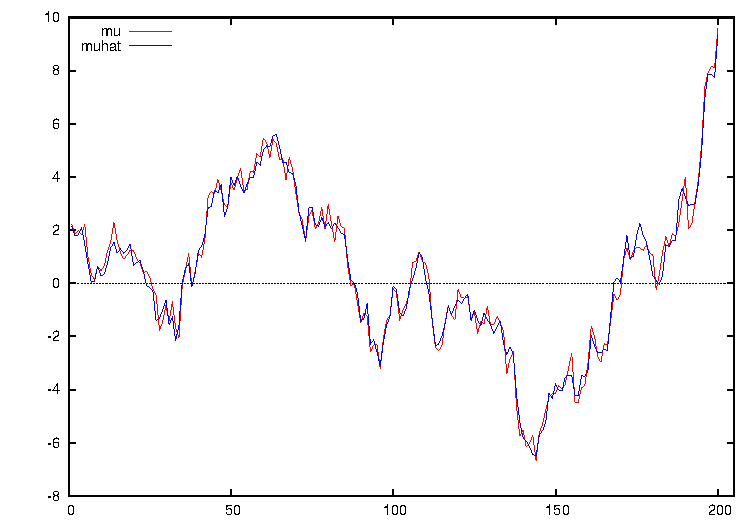
\includegraphics{figures/local_level}
  \caption{Local level model: $\mu_t$ and its smoothed estimate}
  \label{fig:loclev}
\end{figure}
By appending the following code snippet to the example in
Table~\ref{script:loclev}, one may check the results against the
\textsf{R} command \texttt{StructTS}.

\begin{code}
foreign language=R --send-data
  y <- gretldata[,"y"]
  a <- StructTS(y, type="level")
  a
  StateFromR <- as.ts(tsSmooth(a))
  gretl.export(StateFromR)
end foreign

append @dotdir/StateFromR.csv

ols Uhat 0 StateFromR --simple
\end{code}




\chapter{Numerical methods}
\label{chap-numerical}

Several functions are available to aid in the construction of
special-purpose estimators: one group of functions are used to
maximize user-supplied functions via numerical methods: BFGS,
Newton--Raphson and Simulated Annealing.  Another relevant function is
\texttt{fdjac}, which produces a forward-difference approximation to
the Jacobian.

\section{BFGS}
\label{sec:BFGSmax}

The \texttt{BFGSmax} function has two required arguments: a vector
holding the initial values of a set of parameters, and a call to a
function that calculates the (scalar) criterion to be maximized, given
the current parameter values and any other relevant data.  If the
object is in fact minimization, this function should return the
negative of the criterion.  On successful completion, \texttt{BFGSmax}
returns the maximized value of the criterion and the matrix given via
the first argument holds the parameter values which produce the
maximum.  It is assumed here that the objective function is a
user-defined function (see Chapter~\ref{chap:functions}) with the
following general set-up:
%
\begin{code}
function scalar ObjFunc (matrix *theta, matrix *X)
  scalar val = ...  # do some computation
  return val
end function
\end{code}

The first argument contains the arguments upon which the maximization
has to take place, while the second argument may be used to hold
``extra'' values that are necessary to compute the objective function,
but are not the variables of the optimization problem. For example, if
the objective function were a loglikelihood, the first argument would
contain the parameters and the second one the data. Or, for more
economic-theory inclined readers, if the objective function were the
utility of a consumer, the first argument would contain the quantities
of goods and the second one their prices and disposable income.

\begin{script}[htbp]
  \caption{Finding the minimum of the Rosenbrock function}
  \label{rosenbrock}
\begin{scode}
function scalar Rosenbrock(matrix *param)
  scalar x = param[1]
  scalar y = param[2]
  return -(1-x)^2 - 100 * (y - x^2)^2
end function

matrix theta = { 0, 0 }

set max_verbose 1
M = BFGSmax(theta, Rosenbrock(&theta))

print theta
\end{scode}
\end{script}

The operation of BFGS can be adjusted using the \texttt{set} variables
\verb+bfgs_maxiter+ and \verb+bfgs_toler+ (see
Chapter~\ref{chap:mle}).  In addition you can provoke verbose output
from the maximizer by assigning a positive value to
\verb|max_verbose|, again via the \cmd{set} command.

The Rosenbrock function is often used as a test problem for
optimization algorithms. It is also known as ``Rosenbrock's Valley''
or ``Rosenbrock's Banana Function'', on account of the fact that its
contour lines are banana-shaped. It is defined by:
%
\[
    f(x,y) = (1 - x)^2 + 100(y - x^2)^2
\]
%
The function has a global minimum at $(x,y) = (1,1)$ where $f(x,y) =
0$.  Example~\ref{rosenbrock} shows a gretl script that
discovers the minimum using \texttt{BFGSmax} (giving a verbose account
of progress). Note that, in this particular case, the function to be
maximized only depends on the parameters, so the second parameter is
omitted from the definition of the function \texttt{Rosenbrock}. 

\subsection{Limited-memory variant}
\label{sec:LBFGS}

See \cite{byrd-etal95} (\ldots FIXME: expand a little here \ldots)

\subsection{Supplying analytical derivatives for BFGS}
\label{sec:BFGSgrad}

An optional third argument to the \texttt{BFGSmax} function enables
the user to supply analytical derivatives of the criterion
function with respect to the parameters (without which a numerical
approximation to the gradient is computed).  This argument is
similar to the second one in that it specifies a function call.
In this case the function that is called must have the following
signature.  

Its first argument should be a pre-defined matrix correctly
dimensioned to hold the gradient; that is, if the parameter vector
contains $k$ elements, the gradient matrix must also be a $k$-vector.
This matrix argument must be given in ``pointer'' form so that its
content can be modified by the function.  (Note that unlike the
parameter vector, where the choice of initial values can be important,
the initial values given to the gradient are immaterial and do not
affect the results.)

In addition the gradient function must have as one of its argument the
parameter vector.  This may be given in pointer form (which enhances
efficiency) but that is not required.  Additional arguments may be
specified if necessary.

Given the current parameter values, the function call must fill out
the gradient vector appropriately.  It is not required that the
gradient function returns any value directly; if it does, that value
is ignored.

Example~\ref{rosen-analytical} illustrates, showing how the Rosenbrock
script can be modified to use analytical derivatives.  (Note that
since this is a minimization problem the values written into
\texttt{g[1]} and \texttt{g[2]} in the function \verb|Rosen_grad| are
in fact the derivatives of the negative of the Rosenbrock function.)

\begin{script}[htbp]
  \caption{Rosenbrock function with analytical gradient}
  \label{rosen-analytical}
\begin{scode}
function scalar Rosenbrock (matrix *param)
  scalar x = param[1]
  scalar y = param[2]
  return -(1-x)^2 - 100 * (y - x^2)^2
end function

function void Rosen_grad (matrix *g, matrix *param)
  scalar x = param[1]
  scalar y = param[2]
  g[1] = 2*(1-x) + 2*x*(200*(y-x^2))
  g[2] = -200*(y - x^2)
end function

matrix theta = { 0, 0 }
matrix grad = { 0, 0 }

set max_verbose 1
M = BFGSmax(theta, Rosenbrock(&theta), Rosen_grad(&grad, &theta))

print theta
print grad
\end{scode}
\end{script}

\section{Newton--Raphson}
\label{sec:newton-raphson}

BFGS, discussed above, is an excellent all-purpose maximizer, and
about as robust as possible given the limitations of digital computer
arithmetic. The Newton--Raphson maximizer is not as robust, but may
converge much faster than BFGS for problems where the maximand is
reasonably well behaved---in particular, where it is anything like
quadratic (see below). The case for using Newton--Raphson is enhanced
if it is possible to supply a function to calculate the Hessian
analytically.

The gretl function \texttt{NRmax}, which implements the
Newton--Raphson method, has a maximum of four arguments. The first two
(required) arguments are exactly as for BFGS: an initial parameter
vector, and a function call which returns the maximand given the
parameters. The (optional) third argument is again as in BFGS: a
function call that calculates the gradient. Specific to \texttt{NRmax}
is an optional fourth argument, namely a function call to calculate
the (negative) Hessian. The first argument of this function must be a
pre-defined matrix of the right dimension to hold the Hessian---that
is, a $k \times k$ matrix, where $k$ is the length of the parameter
vector---given in ``pointer'' form. The second argument should be
the parameter vector (optionally in pointer form). Other data may be
passed as additional arguments as needed. Similarly to the case with
the gradient, if the fourth argument to \texttt{NRmax} is omitted then
a numerical approximation to the Hessian is constructed.

What is ultimately required in Newton--Raphson is the negative inverse
of the Hessian. Note that if you give the optional fourth argument,
your function should compute the negative Hessian, but should not
invert it; \texttt{NRmax} takes care of inversion, with special
handling for the case where the matrix is not negative definite, which
can happen far from the maximum.

Script~\ref{rosen-newton} extends the Rosenbrock example, using
\texttt{NRmax} with a function \verb+Rosen_hess+ to compute the
Hessian. The functions \texttt{Rosenbrock} and \verb+Rosen_grad+ are
just the same as in Example~\ref{rosen-analytical} and are omitted for
brevity.

\begin{script}[htbp]
  \caption{Rosenbrock function via Newton--Raphson}
  \label{rosen-newton}
\begin{scode}
function void Rosen_hess (matrix *H, matrix *param)
  scalar x = param[1]
  scalar y = param[2]
  H[1,1] = 2 - 400*y + 1200*x^2
  H[1,2] = -400*x
  H[2,1] = -400*x
  H[2,2] = 200
end function

matrix theta = { 0, 0 }
matrix grad = { 0, 0 }
matrix H = zeros(2, 2)

set max_verbose 1
M = NRmax(theta, Rosenbrock(&theta), Rosen_grad(&grad, &theta), 
          Rosen_hess(&H, &theta))

print theta
print grad
\end{scode}
\end{script}

The idea behind Newton--Raphson is to exploit a quadratic
approximation to the maximand, under the assumption that it is
concave. If this is true, the method is very effective. However, if
the algorithm happens to evaluate the function at a point where the
Hessian is not negative definite, things may go wrong. Script
\ref{ex:BFGS-vs-NR} exemplifies this by using a normal density, which
is concave in the interval $(-1,1)$ and convex elsewhere. If the
algorithm is started from within the interval everything goes well
and NR is (slightly) more effective than BFGS. If, however, the
Hessian is positive at the starting point BFGS converges with only
little more difficulty, while Newton--Raphson fails.

\begin{script}[htbp]
  \caption{Maximization of a Gaussian density}
  \label{ex:BFGS-vs-NR}
\begin{scode}
function scalar ND(matrix x)
    scalar z = x[1]
    return exp(-0.5*z*z)
end function

set max_verbose 1

x = {0.75}
A = BFGSmax(x, ND(x))

x = {0.75}
A = NRmax(x, ND(x))

x = {1.5}
A = BFGSmax(x, ND(x))

x = {1.5}
A = NRmax(x, ND(x))
\end{scode}
\end{script}


\section{Simulated Annealing}
\label{sec:sim-anneal}

Simulated annealing---as implemented by the gretl function
\texttt{simann}---is not a full-blown maximization method in its own
right, but can be a useful auxiliary tool in problems where
convergence depends sensitively on the initial values of the
parameters. The idea is that you supply initial values and the
simulated annealing mechanism tries to improve on them via controlled
randomization.

The \texttt{simann} function takes up to three arguments. The first
two (required) are the same as for \texttt{BFGSmax} and
\texttt{NRmax}: an initial parameter vector and a function that
computes the maximand. The optional third argument is a positive
integer giving the maximum number of iterations, $n$, which defaults
to 1024.

Starting from the specified point in the parameter space, for each of
$n$ iterations we select at random a new point within a certain radius
of the previous one and determine the value of the criterion at the
new point. If the criterion is higher we jump to the new point;
otherwise, we jump with probability $P$ (and remain at the previous
point with probability $1-P$).  As the iterations proceed, the system
gradually ``cools''---that is, the radius of the random perturbation
is reduced, as is the probability of making a jump when the criterion
fails to increase.

In the course of this procedure $n+1$ points in the parameter space
are evaluated: call them $\theta_i, i=0,\dots,n$, where $\theta_0$ is
the initial value given by the user. Let $\theta^*$ denote the
``best'' point among $\theta_1, \dots, \theta_n$ (highest criterion
value). The value written into the parameter vector on completion is
then $\theta^*$ if $\theta^*$ is better than $\theta_0$, otherwise
$\theta_n$. In other words, failing an actual improvement in the
criterion, \texttt{simann} randomizes the starting point, which may be
helpful in tricky optimization problems.

Example~\ref{ex:simann} shows \texttt{simann} at work as a helper for
\texttt{BFGSmax} in finding the maximum of a bimodal function.
Unaided, \texttt{BFGSmax} requires 60 function evaluations and
55 evaluations of the gradient, while after simulated annealing
the maximum is found with 7 function evaluations and 6 evaluations
of the gradient.\footnote{Your mileage may vary: these figures
are somewhat compiler- and machine-dependent.}

\begin{script}[htbp]
  \caption{BFGS with initialization via Simulated Annealing}
  \label{ex:simann}
\begin{scode}
function scalar bimodal (matrix x, matrix A)
    scalar ret = exp(-qform((x-1)', A))
    ret += 2*exp(-qform((x+4)', A))
    return ret
end function

set seed 12334
set max_verbose on

scalar k = 2
matrix A = 0.1 * I(k)
matrix x0 = {3; -5}

x = x0
u = BFGSmax(x, bimodal(x, A))
print x

x = x0
u = simann(x, bimodal(x, A), 1000)
print x
u = BFGSmax(x, bimodal(x, A))
print x
\end{scode}
\end{script}

\section{Computing a Jacobian}
\label{sec:fdjac}

Gretl offers the possibility of differentiating numerically a
user-defined function via the \texttt{fdjac} function.

This function takes two arguments: an $n \times 1$ matrix holding
initial parameter values and a function call that calculates and
returns an $m \times 1$ matrix, given the current parameter values and
any other relevant data.  On successful completion it returns an $m
\times n$ matrix holding the Jacobian.  For example,
%
\begin{code}
matrix Jac = fdjac(theta, SumOC(&theta, &X))
\end{code}
where we assume that \texttt{SumOC} is a user-defined function with
the following structure:
%
\begin{code}
function matrix SumOC (matrix *theta, matrix *X)
  matrix V = ...  # do some computation
  return V
end function
\end{code}

This may come in handy in several cases: for example, if you use
\texttt{BFGSmax} to estimate a model, you may wish to calculate a
numerical approximation to the relevant Jacobian to construct a
covariance matrix for your estimates.

Another example is the delta method: if you have a consistent
estimator of a vector of parameters $\hat{\theta}$, and a consistent
estimate of its covariance matrix $\Sigma$, you may need to compute
estimates for a nonlinear continuous transformation $\psi =
g(\theta)$. In this case, a standard result in asymptotic theory is
that
\[
\left\{
    \begin{array}{c}
      \hat{\theta} \convp \theta \\ 
      \sqrt{T} \left( \hat{\theta} - \theta \right) \convd N(0, \Sigma)
    \end{array}
\right\}
    \Longrightarrow
\left\{
    \begin{array}{c}
      \hat{\psi} = g(\hat{\theta}) \convp \psi = g(\theta) \\ 
      \sqrt{T} \left( \hat{\psi} - \psi \right) \convd N(0, J
      \Sigma J')
    \end{array}
\right\}
\]
where $T$ is the sample size and $J$ is the Jacobian
$\left.\pder{g(x)}{x}\right|_{x = \theta}$.

\begin{script}[htbp]
  \caption{Delta Method}
  \label{delta-method}
\begin{scode}
function matrix MPC(matrix *param, matrix *Y)
  beta = param[2]
  gamma = param[3]
  y = Y[1]
  return beta*gamma*y^(gamma-1)
end function

# William Greene, Econometric Analysis, 5e, Chapter 9
set echo off
set messages off
open greene5_1.gdt

# Use OLS to initialize the parameters
ols realcons 0 realdpi --quiet
genr a = $coeff(0)
genr b = $coeff(realdpi)
genr g = 1.0

# Run NLS with analytical derivatives
nls realcons = a + b * (realdpi^g)
  deriv a = 1
  deriv b = realdpi^g
  deriv g = b * realdpi^g * log(realdpi)
end nls

matrix Y = realdpi[2000:4]
matrix theta = $coeff
matrix V = $vcv

mpc = MPC(&theta, &Y)
matrix Jac = fdjac(theta, MPC(&theta, &Y))
Sigma = qform(Jac, V)

printf "\nmpc = %g, std.err = %g\n", mpc, sqrt(Sigma)
scalar teststat = (mpc-1)/sqrt(Sigma)
printf "\nTest for MPC = 1: %g (p-value = %g)\n", \
	teststat, pvalue(n,abs(teststat))
\end{scode}
\end{script}

Script \ref{delta-method} exemplifies such a case: the example is
taken from \cite{greene03}, section 9.3.1. The slight differences
between the results reported in the original source and what
gretl returns are due to the fact that the Jacobian is computed
numerically, rather than analytically as in the book.

On the subject of numerical versus analytical derivatives, one may
wonder what difference it makes to use one method or another. Simply
put, the answer is: analytical derivatives may be painful to derive
and to translate into code, but in most cases they are much faster
than using \cmd{fdjac}; as a consequence, if you need to use
derivatives as part of an algorithm that requires iteration (such as
numerical optimization, or a Monte Carlo experiment), you'll
definitely want to use analytical derivatives.

Analytical derivatives are also, in most cases, more precise than
numerical ones, but this advantage may or may not be negligible in
practice depending on the practical details: the two fundamental
aspects to take in consideration are nonlinearity and machine precision.

As an example, consider the derivative of a highly nonlinear function
such as the matrix inverse. In order to keep the example simple, let's
focus on $2 \times 2$ matrices and define the function
\begin{code}
function matrix vecinv(matrix x)
    A = mshape(x,2,2)
    return vec(inv(A))'
end function
\end{code}
which, given $\mathrm{vec}(A)$, returns $\mathrm{vec}(A^{-1})$. As is
well known (see for example \cite{magneu88}),
\[
  \frac{\partial \mathrm{vec}(A^{-1})}{\partial \mathrm{vec}(A)} 
  = - (A^{-1})' \otimes (A^{-1}),
\]
which is rather easy to code in \app{hansl} as
\begin{code}
function matrix grad(matrix x)
    iA = inv(mshape(x,2,2))
    return -iA' ** iA
end function  
\end{code}
Using the \cmd{fdjac} function to obtain the same result is even
easier: you just invoke it like
\begin{code}
fdjac(a, "vecinv(a)")  
\end{code}

In order to see what the difference is, in terms of precision, between
analytical and numerical Jacobians, let's start from $A =
\left[\begin{array}{cc} 2 & 1 \\ 1 & 1 \end{array}\right]$. The
following code
\begin{code}
a = {2; 1; 1; 1}
ia = vecinv(a)
ag = grad(a)
ng = fdjac(a, "vecinv(a)")
dg = ag - ng
print ag ng dg  
\end{code}
gives
\begin{code}
ag (4 x 4)

  -1    1    1   -1 
   1   -2   -1    2 
   1   -1   -2    2 
  -1    2    2   -4 

ng (4 x 4)

  -1    1    1   -1 
   1   -2   -1    2 
   1   -1   -2    2 
  -1    2    2   -4 

dg (4 x 4)

 -3.3530e-08  -3.7251e-08  -3.7251e-08  -3.7255e-08 
  2.6079e-08   5.2150e-08   3.7251e-08   6.7060e-08 
  2.6079e-08   3.7251e-08   5.2150e-08   6.7060e-08 
 -2.2354e-08  -5.9600e-08  -5.9600e-08  -1.4902e-07 
\end{code}
in which the analytically-computed derivative and its numerical
approximation are essentially the same. If, however, you set $A =
\left[\begin{array}{cc} 1.0001 & 1 \\ 1 & 1 \end{array}\right]$ you
end up evaluating the function at a point in which the function itself
is considerably more nonlinear since the matrix is much closer to
being singular. As a consequence, the numerical approximation becomes
much less satisfactory:
\begin{code}
ag (4 x 4)

 -1.0000e+08   1.0000e+08   1.0000e+08  -1.0000e+08 
  1.0000e+08  -1.0001e+08  -1.0000e+08   1.0001e+08 
  1.0000e+08  -1.0000e+08  -1.0001e+08   1.0001e+08 
 -1.0000e+08   1.0001e+08   1.0001e+08  -1.0002e+08 

ng (4 x 4)

 -9.9985e+07   1.0001e+08   1.0001e+08  -9.9985e+07 
  9.9985e+07  -1.0002e+08  -1.0001e+08   9.9995e+07 
  9.9985e+07  -1.0001e+08  -1.0002e+08   9.9995e+07 
 -9.9985e+07   1.0002e+08   1.0002e+08  -1.0001e+08 

dg (4 x 4)

     -14899.      -14901.      -14901.      -14900. 
      14899.       14903.       14901.       14902. 
      14899.       14901.       14903.       14902. 
     -14899.      -14903.      -14903.      -14903. 
\end{code}
Moreover, machine precision may have its impact: if you take $A =
0.00001 \times \left[\begin{array}{cc} 2 & 1\\ 1 &
    1 \end{array}\right]$, the matrix itself is not singular at
all, but the order of magnitude of its elements is close enough to
machine precision to provoke problems:
\begin{code}
ag (4 x 4)

 -1.0000e+10   1.0000e+10   1.0000e+10  -1.0000e+10 
  1.0000e+10  -2.0000e+10  -1.0000e+10   2.0000e+10 
  1.0000e+10  -1.0000e+10  -2.0000e+10   2.0000e+10 
 -1.0000e+10   2.0000e+10   2.0000e+10  -4.0000e+10 

ng (4 x 4)

 -1.0000e+10   1.0000e+10   1.0000e+10  -1.0000e+10 
  1.0000e+10  -2.0000e+10  -1.0000e+10   2.0000e+10 
  1.0000e+10  -1.0000e+10  -2.0000e+10   2.0000e+10 
 -1.0000e+10   2.0000e+10   2.0000e+10  -4.0000e+10 

dg (4 x 4)

     -488.30      -390.60      -390.60      -195.33 
      634.79       781.21       390.60       585.98 
      634.79       488.26       683.55       585.98 
     -781.27      -976.52      -781.21      -1367.3 
\end{code}

%%% Local Variables: 
%%% mode: latex
%%% TeX-master: "gretl-guide"
%%% End: 

\chapter{Variabili dipendenti discrete e censurate}
\label{chap:discr-models}

\section{Modelli logit e probit}
\label{sec:logit-probit}

Capita spesso che si voglia specificare e stimare un modello in cui la variabile
dipendente non � continua  ma discreta. Un esempio tipico � quello di un modello
in cui la variabile dipendente � lo stato lavorativo di un individuo (1 =
occupato, 0 = disoccupato). Un modo comodo per formalizzare questa situazione
consiste nel considerare la variabile $y_i$ come una variabile aleatoria di
Bernoulli e analizzarne la distribuzione condizionata alle variabili esplicative
$x_i$, ossia
\begin{equation}
  \label{eq:qr-Bernoulli}
  y_i = \left\{ 
    \begin{array}{ll}
      1 & P_i \\ 0 & 1 - P_i
    \end{array}
    \right. 
\end{equation}
%
dove $P_i = P(y_i = 1 | x_i) $ � una funzione delle variabili esplicative $x_i$.

Nella maggior parte dei casi, la funzione $P_i$ � una funzione di ripartizione
$F$, applicata a una combinazione lineare delle $x_i$. Nel modello probit, si usa la
funzione di ripartizione normale, mentre il modello logit usa la funzione
logistica $\Lambda()$. Quindi si ha
%
\begin{eqnarray}
  \label{eq:qr-link}
  \textrm{probit} & \qquad & P_i = F(z_i) = \Phi(z_i)  \\
  \textrm{logit}  & \qquad & P_i = F(z_i) = \Lambda(z_i) = \frac{1}{1 + e^{-z_i}} \\
  & &z_i = \sum_{j=1}^k x_{ij} \beta_j
\end{eqnarray}
%
dove $z_i$ � chiamata la funzione \emph{indicatrice}. Si noti che in questo
caso, i coefficienti $\beta_j$ non possono essere interpretati come derivate
parziali di $E(y_i | x_i)$ rispetto a $x_{ij}$. Comunque, per un dato valore
di $x_i$ � possibile calcolare il vettore delle ``pendenze'', ossia
\[
  \mathrm{slope}_j(\bar{x}) = \left. \pder{F(z)}{x_j} \right|_{z =
    \bar{z}}
\]
\app{Gretl} calcola automaticamente le pendenze assegnando a ogni variabile
esplicativa un valore pari alla sua media.

Un modo equivalente di formulare questo modello consiste nell'ipotizzare
l'esistenza di una variabile non osservata $y^*_i$ che pu� essere descritta nel
modo seguente:
%
\begin{equation}
  \label{eq:qr-latent}
  y^*_i = \sum_{j=1}^k x_{ij} \beta_j + \varepsilon_i = z_i  +
  \varepsilon_i
\end{equation}
%
Si osserva $y_i = 1$ quando $y^*_i > 0$ e $y_i = 0$ altrimenti. Se si assume
$\varepsilon_i$ come normale, si ottiene il modello probit, mentre il modello
logit assume che la funzione di densit� di $\varepsilon_i$ sia
%
\[
  \lambda(\varepsilon_i) =
  \pder{\Lambda(\varepsilon_i)}{\varepsilon_i} =
  \frac{e^{-\varepsilon_i}}{(1 + e^{-\varepsilon_i})^2}
\]
%
\app{gretl} stima sia il modello probit che quello logit col metodo della
massima verosimiglianza; poich� le equazioni degli score non hanno una soluzione
in forma chiusa, vengono usate procedure di ottimizzazione numerica. La maggior
parte delle volte queste richiedono poche iterazioni per raggiungere la
convergenza, ma � possibile visualizzare i dettagli dell'algoritmo di
massimizzazione usando l'opzione \texttt{--verbose}.

\begin{script}[htbp]
  \caption{Stima di semplici modelli logit e probit}
  \label{simple-QR}
\begin{scode}
open greene19_1

logit GRADE const GPA TUCE PSI
probit GRADE const GPA TUCE PSI
\end{scode}
\end{script}

Come esempio, riproduciamo i risultati esposti nel capitolo 21 di Greene (2000),
dove viene valutata l'efficacia di un programma per insegnare l'economia
osservando i miglioramenti nei voti degli studenti.
Eseguendo il codice contenuto nell'esempio \ref{simple-QR} si ottengono i seguenti risultati:
\begin{code}

Modello 1: Stime Logit usando le 32 osservazioni 1-32
Variabile dipendente: GRADE

      VARIABILE      COEFFICIENTE       ERRORE STD    STAT T       PENDENZA
                                                                  (alla media)
  const               -13,0213           4,93132      -2,641
  GPA                   2,82611          1,26294       2,238      0,533859   
  TUCE                  0,0951577        0,141554      0,672      0,0179755  
  PSI                   2,37869          1,06456       2,234      0,449339   

  Media di GRADE = 0,344
  Numero dei casi 'previsti correttamente' = 26 (81,2%)
  f(beta'x) nella media delle variabili indipendenti = 0,189
  Pseudo-R-quadro di McFadden = 0,374038
  Log-verosimiglianza = -12,8896
  Test del rapporto di verosimiglianza: Chi-quadro(3) = 15,4042 (p-value 0,001502)
  Criterio di informazione di Akaike (AIC) = 33,7793
  Criterio bayesiano di Schwarz (BIC) = 39,6422
  Criterio di Hannan-Quinn (HQC) = 35,7227

              Previsto
                0    1
  Effettivo 0  18    3
            1   3    8

Modello 2: Stime Probit usando le 32 osservazioni 1-32
Variabile dipendente: GRADE

      VARIABILE      COEFFICIENTE       ERRORE STD    STAT T       PENDENZA
                                                                  (alla media)
  const                -7,45232          2,54247      -2,931
  GPA                   1,62581          0,693883      2,343      0,533347   
  TUCE                  0,0517288        0,0838903     0,617      0,0169697  
  PSI                   1,42633          0,595038      2,397      0,467908   

  Media di GRADE = 0,344
  Numero dei casi 'previsti correttamente' = 26 (81,2%)
  f(beta'x) nella media delle variabili indipendenti = 0,328
  Pseudo-R-quadro di McFadden = 0,377478
  Log-verosimiglianza = -12,8188
  Test del rapporto di verosimiglianza: Chi-quadro(3) = 15,5459 (p-value 0,001405)
  Criterio di informazione di Akaike (AIC) = 33,6376
  Criterio bayesiano di Schwarz (BIC) = 39,5006
  Criterio di Hannan-Quinn (HQC) = 35,581

              Previsto
                0    1
  Effettivo 0  18    3
            1   3    8

\end{code}

In questo contesto, la funzione accessoria \verb+$uhat+ assume un
significato speciale: produce i residui generalizzati come sono definiti in
Gourieroux \textit{et al} (1987), che possono essere interpretati come stimatori non distorti dei
disturbi latenti $\varepsilon_t$. Questi sono definiti come
%
\begin{equation}
  \label{eq:QR-genres}
  u_i = \left\{
    \begin{array}{ll}
      y_i - \hat{P}_i & \textrm{per il modello logit} \\
      y_i\cdot \frac{\phi(\hat{z}_i)}{\Phi(\hat{z}_i)} - 
      ( 1 - y_i ) \cdot \frac{\phi(\hat{z}_i)}{1 - \Phi(\hat{z}_i)}
      & \textrm{per il modello probit} \\
    \end{array}
    \right.
\end{equation}

Tra l'altro, i residui generalizzati sono spesso usati a scopo diagnostico; ad
esempio, � molto facile costruire un test per variabili omesse
equivalente al test LM usato tipicamente nel contesto della regressione lineare:
l'esempio \ref{QR-add} mostra come eseguire un test per l'aggiunta di una
variabile.

\begin{script}[htbp]
  \caption{Test per l'aggiunta di una variabile in un modello probit}
  \label{QR-add}
\begin{scode}
open greene19_1

probit GRADE const GPA PSI
series u = $uhat 

ols u const GPA PSI TUCE -q
printf "Test per l'aggiunta della variabile TUCE:\n"
printf "Rsq * T = %g (p. val. = %g)\n", $trsq, pvalue(X,1,$trsq) 
\end{scode}
\end{script}

\subsection{Modelli ordinati}
\label{sec:ordered}

Questi modelli sono semplici variazioni sui normali modelli logit/probit,
utilizzati di solito nei casi in cui la variabile dipendente assume valori
discreti e ordinati, non necessariamente quantitativi. Ad esempio, questi
modelli possono essere applicati per analizzare casi in cui la variabile
dipendente � un giudizio qualitativo come ``Buono'', ``Medio'', ``Scarso''.
Ipotizzando di avere $p$ categorie, la probabilit� che l'individuo $i$ ricada
nella $j$-esima categoria � dato da
%
\begin{equation}
  \label{eq:QR-ordered}
  P(y_i = j | x_i) = \left\{
    \begin{array}{ll}
      F(z_i + \mu_0) & \textrm{per } j = 0 \\
      F(z_i + \mu_j) -  F(z_i + \mu_{j-1}) & \textrm{per } 0 < j < p \\
      1 -  F(z_i + \mu_{p-1}) & \textrm{per } j = p 
    \end{array}
    \right.
\end{equation}
%
I parametri ignoti $\mu_j$ sono chiamati ``punti di taglio'' e sono stimati
insieme ai $\beta$'. Ai fini dell'identificazione, $\mu_0$ � ipotizzato pari a
0.  In termini della variabile non osservata $y^*_i$, il modello pu� essere
espresso in modo equivalente come
$P(y_i = j | x_i) = P(\mu_{j-1} \le y^*_i < \mu_j)$. 

\begin{script}[htbp]
  \caption{Modello probit ordinato}
  \label{ex:oprobit}
\begin{scode}
open pension.gdt
series pctstck = pctstck/50
discrete pctstck
probit pctstck const choice age educ female black married finc25 finc35 \
  finc50 finc75 finc100 finc101 wealth89 prftshr
\end{scode}
\end{script}

Per applicare questi modelli, la variabile dipendente deve essere marcata come
discreta e il suo valore minimo deve essere pari a 0. L'esempio \ref{ex:oprobit}
riproduce la stima proposta nel capitolo 15 di Wooldridge (2002a). Si noti che
\app{gretl} non fornisce un comando separato per i modelli ordinati: i comandi
\texttt{logit} e \texttt{probit} stimano automaticamente le versioni ordinate se
la variabile dipendente non � binaria (a patto che sia stata marcata in
precedenza come discreta).

Dopo aver stimato modelli ordinati, la variabile \verb+$uhat+ contiene i
residui generalizzati, come avviene per i modelli binari; in pi�, la variabile
\verb+$yhat+ contiene $\hat{z}_i$, cos� � possibile calcolare una stima non
distorta della variabile latente $y^*_i$ semplicemente facendo l'addizione delle
due.

\subsection{Logit multinomiale}
\label{sec:mlogit}

Quando la variabile dipendente non � binaria e non ha un ordinamento naturale,
si usano modelli \emph{multinomiali}. \app{Gretl} non fornisce ancora
un'implementazione interna per questo tipo di modelli, ma alcuni casi semplici
possono essere gestiti usando il comando \texttt{mle} command (si veda il
capitolo \ref{chap:mle}). Di seguito viene presentato un esempio di modello
logit multinomiale. Si assuma che la variabile dipendente $y_i$ possa avere
valori interi $0,1,\dots p$.  La probabilit� che sia $y_i = k$ � data da
\[
  P(y_i = k |  x_i) = \frac{\exp(x_i \beta_k)}{\sum_{j=0}^p \exp(x_i \beta_j)}
\]
Ai fini dell'identificazione del modello, uno dei valori deve essere preso come
quello ``di riferimento''; di solito si assume che valga $\beta_0 = 0$, nel cui caso
\[
  P(y_i = k |  x_i) = \frac{\exp(x_i \beta_k)}{1 + \sum_{j=1}^p \exp(x_i \beta_j)} 
\]
e
\[
  P(y_i = 0 |  x_i) = \frac{1}{1 + \sum_{j=1}^p \exp(x_i \beta_j)} .
\]

L'esempio~\ref{ex:mlogit} riproduce la Tabella 15.2 di Wooldridge (2002a),
che si basa su dati sulle scelte di carriera contenuti in Keane e Wolpin (1997).
La variabile dipendente � lo stato occupazionale di un individuo (0 = studente;
1 = non studente e non occupato; 2 = occupato) e le variabili esplicative sono
il livello di educazione e l'esperienza lavorativa (in livelli e nei quadrati),
oltre a una variabile binaria ``oscura''. Il dataset completo � di tipo panel,
ma l'analisi presentata di seguito riguarda solo i dati del 1987. Per i dettagli
sulle operazioni matriciali usate in questo script, si veda il
capitolo~\ref{chap:matrices}.

\begin{script}[htbp]
  \caption{Logit multinomiale}
  \label{ex:mlogit}
\begin{scode}
function mlogitlogprobs(series y, matrix X, matrix theta)

  scalar n = max(y)
  scalar k = cols(X)
  matrix b = mshape(theta,k,n)

  matrix tmp = X*b
  series ret = -ln(1 + sumr(exp(tmp)))

  loop for i=1..n --quiet
    series x = tmp[,i]
    ret += (y=$i) ? x : 0 
  end loop

  return series ret

end function

open Keane.gdt
status = status-1 # dep. var. must be 0-based
smpl (year=87 & ok(status)) --restrict

matrix X = { educ exper expersq black const }
scalar k = cols(X)
matrix theta = zeros(2*k, 1)

mle loglik = mlogitlogprobs(status,X,theta)
  params theta
end mle --verbose --hessian
\end{scode}
%$
\end{script}


\section{Il modello Tobit}
\label{sec:tobit}

Il modello Tobit viene usato quando la variabile dipendente di un modello �
censurata\footnote{Stiamo assumendo che i dati siano censurati per quanto riguarda
  i valori inferiori a zero. I casi di censura per valori maggiori di zero,
  o in corrispondenza di valori diversi da zero, possono essere trattati facilmente
  ridefinendo la variabile dipendente. Il caso pi� generale di censura da due
  lati non � contemplato automaticamente da \app{gretl}, ma � possibile stimare
  tali modelli usando il comando \texttt{mle} (si veda il capitolo
  \ref{chap:mle}).}.
Si ipotizzi che una variabile latente $y^*_i$ possa essere descritta
come
%
\[
  y^*_i = \sum_{j=1}^k x_{ij} \beta_j + \varepsilon_i ,
\]
%
dove $\varepsilon_i \sim N(0,\sigma^2)$. Se le $y^*_i$ fossero osservabili, i
parametri del modello potrebbero essere stimati con i minimi quadrati ordinari.
Al contrario, si supponga di poter osservare $y_i$, definita
come
%
\begin{equation}
  \label{eq:tobit}
  y_i = \left\{ 
    \begin{array}{ll} 
      y^*_i & \mathrm{for} \quad y^*_i > 0 \\ 
      0 & \mathrm{for} \quad y^*_i \le 0 
    \end{array}
    \right. 
\end{equation}
%
In questo caso, regredire $y_i$ sulle $x_i$ non produce stime consistenti dei
parametri $\beta$, perch� la media condizionale $E(y_i|x_i)$ non � pari a $\sum_{j=1}^k x_{ij}
\beta_j$. Come si pu� dimostrare, nemmeno restringere il campione alle
osservazioni diverse da zero non produrrebbe stime consistenti. La soluzione sta
nello stimare i parametri con la massima verosimiglianza. La sintassi �
semplicemente
%
\begin{code}
tobit depvar indvars
\end{code}

Come al solito, � possibile visualizzare i progressi dell'algoritmo di
massimizzazione usando l'opzione \texttt{--verbose} e \verb+$uhat+
contiene i residui generalizzati. Si noti che in questo caso il residuo
generalizzato � definito come $\hat{u}_i = E(\varepsilon_i | y_i = 0)$ per
le osservazioni censurate, quindi l'uguaglianza $\hat{u}_i = y_i - \hat{y}_i$
vale solo per le osservazioni non censurate, ossia quando vale $y_i>0$.

Un'importante differenza tra lo stimatore Tobit e quello OLS � che le
conseguenze della non-normalit� del termine di disturbo sono molto pi� severe,
visto che la non-normalit� implica la non consistenza per lo stimatore Tobit.
Per questo motivo, fra i risultati del modello Tobit viene mostrato anche il
test di normalit� di Chesher--Irish (1987).

\subsection{Modello di selezione del campione}
\label{sec:heckit}

Nel modello di selezione del campione (noto anche come modello ``Tobit II''),
esistono due variabili latenti:
%
\begin{eqnarray}
  \label{eq:heckit1}
  y^*_i & = & \sum_{j=1}^k x_{ij} \beta_j + \varepsilon_i \\
  \label{eq:heckit2}
  s^*_i & = & \sum_{j=1}^p z_{ij} \gamma_j + \eta_i 
\end{eqnarray}
%
e la regola di osservazione � data da
%
\begin{equation}
  \label{eq:tobitII}
  y_i = \left\{ 
    \begin{array}{ll} 
      y^*_i & \mathrm{for} \quad s^*_i > 0 \\ 
      \diamondsuit & \mathrm{for} \quad s^*_i \le 0 
    \end{array}
    \right. 
\end{equation}

In questo contesto, il simbolo $\diamondsuit$ indica che per alcune osservazioni
non sono disponibili dati per $y$: $y_i$ pu� essere 0 o mancante, o assumere
qualsiasi altro valore. Di solito si usa una variabile dummy $d_i$ per escludere
le osservazioni censurate.

Una delle applicazioni pi� popolari di questo modello in econometria prevede
un'equazione dei salari e un'equazione della partecipazione alla forza lavoro:
viene osservato solo il salario delle persone occupate. Se $y^*_i$ e $s^*_i$ fossero
(condizionalmente) indipendenti, non ci sarebbe motivo per non usare lo
stimatore OLS per stimare l'equazione (\ref{eq:heckit1}); ma in altri casi, lo
stimatore OLS non produce stime consistenti dei parametri $\beta_j$.

Visto che l'indipendenza condizionale tra $y^*_i$ e $s^*_i$ � equivalente
all'indipendenza condizionale tra $\varepsilon_i$ e $\eta_i$, si pu� modellare
la co-dipendenza tra $\varepsilon_i$ e $\eta_i$ come
\[
  \varepsilon_i = \lambda \eta_i + v_i ;
\]
sostituendo l'espressione precedente nella (\ref{eq:heckit1}), si ottiene il
modello che viene effettivamente stimato:
\[
  y_i = \sum_{j=1}^k x_{ij} \beta_j + \lambda \hat{\eta}_i + v_i ,
\]
quindi l'ipotesi per cui la censura non ha importanza equivale all'ipotesi
$H_0: \lambda = 0$, che pu� essere testata facilmente.

I parametri possono essere stimati con la massima verosimiglianza nell'ipotesi
di normalit� congiunta di $\varepsilon_i$ e $\eta_i$, ma un metodo alternativo
molto usato � il cosidetto stimatore \emph{Heckit}, che prende il
nome da Heckman (1979). La procedura pu� essere schematizzata nel modo seguente:
per prima cosa viene stimato un modello probit per l'equazione (\ref{eq:heckit2});
quindi, vengono inseriti i residui generalizzati nell'equazione (\ref{eq:heckit1})
per correggere gli effetti della selezione del campione.

\app{Gretl} fornisce il comando \texttt{heckit} per eseguire la stima; la
sintassi �
%
\begin{code}
heckit y X ; d Z
\end{code}
%
dove \texttt{y} � la variabile dipendente, \texttt{X} � una lista di
regressori, \texttt{d} � una variabile dummy che vale 1 per le osservazioni non
censurate, e \texttt{Z} � una lista di variabili esplicative per l'equazione di
censura.

Visto che quello della massima verosimiglianza � il metodo scelto pi� spesso,
per impostazione predefinita \app{gretl} calcola le stime ML. Le stime
Heckit a due passi si ottengono usando l'opzione \texttt{--two-step}. Dopo la
stima, la variabile \verb|$uhat| contiene i residui generalizzati. Come nel
modello Tobit ordinario, i residui sono pari alla differenza tra i valori
$y_i$ effettivi e stimati solo per le osservazioni non censurate (quelle per cui
vale $d_i = 1$).

L'esempio \ref{ex:heckit} mostra due stime dal dataset usato in
Mroz (1987): la prima replica la tabella 22.7 di Greene (2003)\footnote{Si noti
che le stime prodotte da \app{gretl} non coincidono con quelle contenute nel
libro, ma con quelle elencate nella pagina degli errata corrige del
libro: \url{http://pages.stern.nyu.edu/~wgreene/Text/Errata/ERRATA5.htm}.},
mentre la seconda replica la tabella 17.1 di Wooldridge (2002a)

\begin{script}[htbp]
  \caption{Modello Heckit}
  \label{ex:heckit}
\begin{scode}
open mroz.gdt

genr EXP2 = AX^2
genr WA2 = WA^2
genr KIDS = (KL6+K618)>0

# Greene's specification

list X = const AX EXP2 WE CIT
list Z = const WA WA2 FAMINC KIDS WE

heckit WW X ; LFP Z --two-step 
heckit WW X ; LFP Z 

# Wooldridge's specification

series NWINC = FAMINC - WW*WHRS
series lww = log(WW)
list X = const WE AX EXP2
list Z = X NWINC WA KL6 K618

heckit lww X ; LFP Z --two-step 
\end{scode}
\end{script}

%\section{Count data}
%\label{sec:poisson}

%also include example script for negative binomial (done in Vebeek
%example files).



%%% Local Variables: 
%%% mode: latex
%%% TeX-master: "gretl-guide"
%%% End: 

\chapter{Quantile regression}
\label{chap:quantreg}

\section{Introduction}
\label{sec:rq-intro}

In Ordinary Least Squares (OLS) regression, the fitted values,
$\hat{y}_i = X_i\hat{\beta}$, represent the \emph{conditional mean} of
the dependent variable---conditional, that is, on the regression
function and the values of the independent variables.  In median
regression, by contrast and as the name implies, fitted values
represent the \emph{conditional median} of the dependent variable.  It
turns out that the principle of estimation for median regression is
easily stated (though not so easily computed), namely, choose
$\hat{\beta}$ so as to minimize the sum of absolute residuals.  Hence
the method is known as Least Absolute Deviations or LAD.  While the OLS
problem has a straightforward analytical solution, LAD is a linear
programming problem.

Quantile regression is a generalization of median regression: the
regression function predicts the conditional $\tau$-quantile of the
dependent variable---for example the first quartile ($\tau = .25$)
or the ninth decile ($\tau = .90$).

If the classical conditions for the validity of OLS are
satisfied---that is, if the error term is independently and
identically distributed, conditional on $X$---then quantile regression
is redundant: all the conditional quantiles of the dependent variable
will march in lockstep with the conditional mean.  Conversely, if
quantile regression reveals that the conditional quantiles behave in a
manner quite distinct from the conditional mean, this suggests that
OLS estimation is problematic.

As of version 1.7.5, gretl offers quantile regression
functionality (in addition to basic LAD regression, which has been
available since early in gretl's history via the \texttt{lad}
command).\footnote{We gratefully acknowledge our borrowing from the
  \texttt{quantreg} package for GNU \textsf{R} (version 4.17).  The
  core of the \texttt{quantreg} package is composed of Fortran code
  written by Roger Koenker; this is accompanied by various driver and
  auxiliary functions written in the \textsf{R} language by Koenker
  and Martin M\"achler.  The latter functions have been re-worked in C
  for gretl.  We have added some guards against potential
  numerical problems in small samples.}

\section{Basic syntax}

The basic invocation of quantile regression is

\vspace{1em}
\noindent
\qquad \texttt{quantreg} \textsl{tau} \textsl{reglist}
\vspace{1em}

where

\begin{itemize}
\item \textsl{reglist} is a standard \textsf{gretl} regression list
  (dependent variable followed by regressors, including the constant
  if an intercept is wanted); and
\item \textsl{tau} is the desired conditional quantile, in the range
  0.01 to 0.99, given either as a numerical value or the name of a
  pre-defined scalar variable (but see below for a further option).
\end{itemize}

Estimation is via the Frisch--Newton interior point solver
\citep{portnoy97}, which is substantially faster than the
``traditional'' Barrodale--Roberts \citeyearpar{barrodale74} simplex
approach for large problems.

By default, standard errors are computed according to the asymptotic
formula given by \cite{koenker-bassett78}.  Alternatively, if the
\option{robust} option is given, we use the sandwich estimator
developed in \cite{koenker-zhao94}.\footnote{These correspond to the
  \texttt{iid} and \texttt{nid} options in \textsf{R}'s
  \texttt{quantreg} package, respectively.}

\section{Confidence intervals}

An option \option{intervals} is available.  When this is given we
print confidence intervals for the parameter estimates instead of
standard errors.  These intervals are computed using the rank
inversion method and in general they are asymmetrical about the point
estimates---that is, they are not simply ``plus or minus so many
standard errors''.  The specifics of the calculation are inflected by
the \option{robust} option: without this, the intervals are computed
on the assumption of IID errors \citep{koenker94}; with it, they use
the heteroskedasticity-robust estimator developed by
\cite{koenker-machado99}.

By default, 90 percent intervals are produced.  You can change this by
appending a confidence value (expressed as a decimal fraction) to the
intervals option, as in

\vspace{1em}
\noindent
\qquad \texttt{quantreg} \textsl{tau} \textsl{reglist} \verb|--intervals=.95|
\vspace{1em}

When the confidence intervals option is selected, the parameter
estimates are calculated using the Barrodale--Roberts method.  This is
simply because the Frisch--Newton code does not currently support the
calculation of confidence intervals.

Two further details.  First, the mechanisms for generating confidence
intervals for quantile estimates require that the model has at least
two regressors (including the constant).  If the \option{intervals}
option is given for a model containing only one regressor, an error is
flagged.  Second, when a model is estimated in this mode, you can
retrieve the confidence intervals using the accessor \dollar{coeff\_ci}.
This produces a $k \times 2$ matrix, where $k$ is the number of
regressors.  The lower bounds are in the first column, the upper
bounds in the second.  See also section~\ref{sec:bigdata} below.

\section{Multiple quantiles}

As a further option, you can give \textsl{tau} as a matrix---either
the name of a predefined matrix or in numerical form, as in
\verb+{.05, .25, .5, .75, .95}+.  The given model is estimated for all
the $\tau$ values and the results are printed in a special form, as
shown below (in this case the \option{intervals} option was also
given).

{\small
\begin{verbatim}
Model 1: Quantile estimates using the 235 observations 1-235
Dependent variable: foodexp
With 90 percent confidence intervals

      VARIABLE      TAU    COEFFICIENT      LOWER        UPPER

  const             0.05      124.880      98.3021      130.517
                    0.25      95.4835      73.7861      120.098
                    0.50      81.4822      53.2592      114.012
                    0.75      62.3966      32.7449      107.314
                    0.95      64.1040      46.2649      83.5790

  income            0.05     0.343361     0.343327     0.389750
                    0.25     0.474103     0.420330     0.494329
                    0.50     0.560181     0.487022     0.601989
                    0.75     0.644014     0.580155     0.690413
                    0.95     0.709069     0.673900     0.734441
\end{verbatim}
}

The gretl GUI has an entry for Quantile Regression (under
\textsf{/Model/Robust estimation}), and you can select multiple
quantiles there too.  In that context, just give space-separated
numerical values (as per the predefined options, shown in a drop-down
list).  

When you estimate a model in this way most of the standard menu items
in the model window are disabled, but one extra item is
available---graphs showing the $\tau$ sequence for a given coefficient
in comparison with the OLS coefficient.  An example is shown in
Figure~\ref{fig:tau}.  This sort of graph provides a simple means of
judging whether quantile regression is redundant (OLS is fine) or
informative.

In the example shown---based on data on household income and food
expenditure gathered by Ernst Engel (1821--1896)---it seems clear
that simple OLS regression is potentially misleading.  The
``crossing'' of the OLS estimate by the quantile estimates is very
marked.  

\begin{figure}
  \centering
  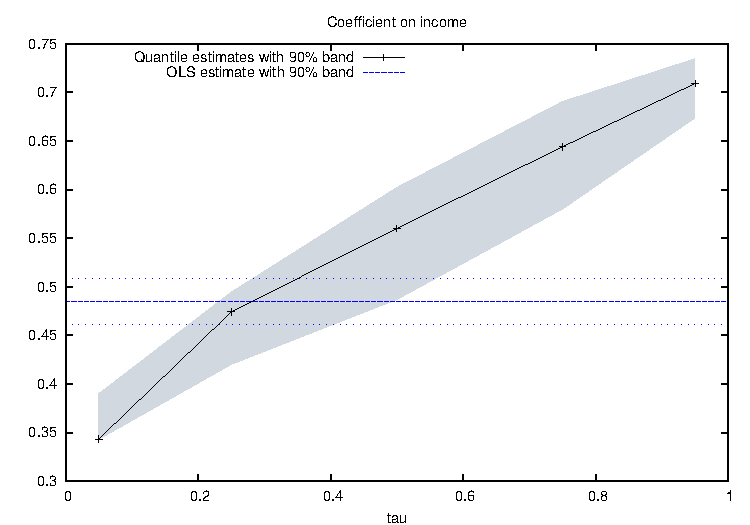
\includegraphics{figures/tau-sequence}
  \caption{Regression of food expenditure on income; Engel's data}
  \label{fig:tau}
\end{figure}

However, it is not always clear what implications should be drawn from
this sort of conflict.  With the Engel data there are two issues to
consider.  First, Engel's famous ``law'' claims an income-elasticity
of food consumption that is less than one, and talk of elasticities
suggests a logarithmic formulation of the model.  Second, there are
two apparently anomalous observations in the data set: household 105
has the third-highest income but unexpectedly low expenditure on food
(as judged from a simple scatter plot), while household 138 (which
also has unexpectedly low food consumption) has much the highest
income, almost twice that of the next highest.

With $n = 235$ it seems reasonable to consider dropping these
observations.  If we do so, and adopt a log--log formulation, we get
the plot shown in Figure~\ref{fig:tau2}.  The quantile estimates still
cross the OLS estimate, but the ``evidence against OLS'' is much less
compelling: the 90 percent confidence bands of the respective
estimates overlap at all the quantiles considered.

\begin{figure}
  \centering
  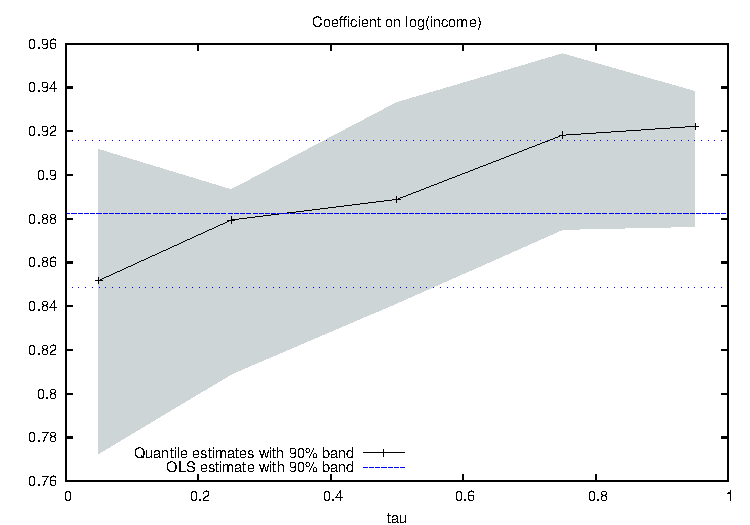
\includegraphics{figures/tau-sequence2}
  \caption{Log--log regression; 2 observations dropped from full Engel data
    set.}
  \label{fig:tau2}
\end{figure}


\section{Large datasets}
\label{sec:bigdata}

As noted above, when you give the \option{intervals} option with the
\texttt{quantreg} command, which calls for estimation of confidence
intervals via rank inversion, gretl switches from the default
Frisch--Newton algorithm to the Barrodale--Roberts simplex method.

This is OK for moderately large datasets (up to, say, a few thousand
observations) but on very large problems the simplex algorithm may
become seriously bogged down.  For example, \cite{koenker-hallock01}
present an analysis of the determinants of birth weights, using 
198377 observations and with 15 regressors.  Generating confidence
intervals via Barrodale--Roberts for a single value of $\tau$ took
about half an hour on a Lenovo Thinkpad T60p with 1.83GHz Intel Core 2
processor.

If you want confidence intervals in such cases, you are advised not to
use the \option{intervals} option, but to compute them using the
method of ``plus or minus so many standard errors''.  (One
Frisch--Newton run took about 8 seconds on the same machine, showing
the superiority of the interior point method.)  The script below
illustrates:
%
\begin{code}
quantreg .10 y 0 xlist
scalar crit = qnorm(.95)
matrix ci = $coeff - crit * $stderr
ci = ci~($coeff + crit * $stderr)
print ci
\end{code}
%
The matrix \texttt{ci} will contain the lower and upper bounds of the
(symmetrical) 90 percent confidence intervals.

To avoid a situation where gretl becomes unresponsive for a very
long time we have set the maximum number of iterations for the
Borrodale--Roberts algorithm to the (somewhat arbitrary) value of
1000.  We will experiment further with this, but for the meantime if
you really want to use this method on a large dataset, and don't mind
waiting for the results, you can increase the limit using the
\texttt{set} command with parameter \verb|rq_maxiter|, as in
\begin{code}
set rq_maxiter 5000
\end{code}












\chapter{Nonparametric methods}
\label{chap-nonparam}

The main focus of gretl is on parametric estimation, but we offer a
selection of nonparametric methods. The most basic of these
%
\begin{itemize}
\item various tests for difference in distribution (Sign test,
  Wilcoxon rank-sum test, Wilcoxon signed-rank test);
\item the Runs test for randomness; and
\item nonparametric measures of association: Spearman's rho and
  Kendall's tau.
\end{itemize}

Details on the above can be found by consulting the help for the
commands \cmd{difftest}, \cmd{runs}, \cmd{corr} and \cmd{spearman}.
In the GUI program these items are found under the \textsf{Tools} menu
and the \textsf{Robust estimation} item under the \textsf{Model} menu.

In this chapter we concentrate on two relatively complex methods for
nonparametric curve-fitting and prediction, namely William
Cleveland's ``loess'' (also known as ``lowess'') and the
Nadaraya--Watson estimator.

\section{Locally weighted regression (loess)}
\label{sec:loess}

Loess \citep{cleveland79} is a nonparametric smoother employing
locally weighted polynomial regression. It is intended to yield an
approximation to $g(\cdot)$ when the dependent variable, $y$, can be
expressed as
\[
y_i = g(x_i) + \epsilon_i
\]
for some smooth function $g(\cdot)$.

Given a sample of $n$ observations on the variables $y$ and $x$, the
procedure is to run a weighted least squares regression (a polynomial
of order $d$ = 0, 1 or 2 in $x$) localized to each data point, $i$. In
each such regression the sample consists of the $r$ nearest neighbors
(in the $x$ dimension) to the point $i$, with weights that are
inversely related to the distance $|x_i - x_k|$, $k=1,\dots,r$. The
predicted value $\hat{y_i}$ is then obtained by evaluating the
estimated polynomial at $x_i$. The most commonly used order is $d=1$.

A bandwidth parameter $0 < q \leq 1$ controls the proportion of the
total number of data points used in each regression; thus $r = qn$
(rounded up to an integer). Larger values of $q$ lead to a smoother
fitted series, smaller values to a series that tracks the actual data
more closely; $0.25 \leq q \leq 0.5$ is often a suitable range.

In gretl's implementation of loess the weighting scheme is
that given by Cleveland, namely,
\[
w_k(x_i) = W(h_i^{-1}(x_k - x_i))
\]
where $h_i$ is the distance between $x_i$ and its $r^{\rm th}$ nearest
neighbor, and $W(\cdot)$ is the tricube function,
\[
W(x) = \begin{cases}
 (1 - |x|^3)^3 & \mbox{for } |x| < 1 \\
  0            & \mbox{for } |x| \geq 1
\end{cases}
\]

The local regression can be made robust via an adjustment based on the
residuals, $e_i = y_i - \hat{y}_i$. Robustness weights, $\delta_k$, are
defined by
\[
\delta_k = B(e_k / 6s)
\]
where $s$ is the median of the $|e_i|$ and $B(\cdot)$ is the
bisquare function,
\[
B(x) = \begin{cases}
 (1 - x^2)^2 & \mbox{for } |x| < 1 \\
  0          & \mbox{for } |x| \geq 1
\end{cases}
\]
The polynomial regression is then re-run using weight
$\delta_kw_k(x_i)$ at $(x_k, y_k)$.

The \texttt{loess()} function in gretl takes up to five
arguments as follows: the $y$ series, the $x$ series, the order $d$,
the bandwidth $q$, and a boolean switch to turn on the robust
adjustment. The last three arguments are optional: if they are omitted
the default values are $d=1$, $q=0.5$ and no robust adjustment. An
example of a full call to \texttt{loess()} is shown below; in this
case a quadratic in $x$ is specified, three quarters of the data
points will be used in each local regression, and robustness is turned
on:
\begin{code}
series yh = loess(y, x, 2, 0.75, 1)
\end{code}

An illustration of loess is provided in Example~\ref{scr:loess-sine}:
we generate a series that has a deterministic sine wave component
overlaid with noise uniformly distributed on $(-1,1)$. Loess is then
used to retrieve a good approximation to the sine function.  The
resulting graph is shown in Figure~\ref{fig:loess-sine}.

\begin{script}[htbp]
  \caption{Loess script}
  \label{scr:loess-sine}
\begin{scode}
nulldata 120
series x = index
scalar n = $nobs
series y = sin(2*pi*x/n) + uniform(-1, 1)
series yh = loess(y, x, 2, 0.75, 0)
gnuplot y yh x --output=display --with-lines=yh
\end{scode}
\end{script}

\begin{figure}[htbp]
  \centering
  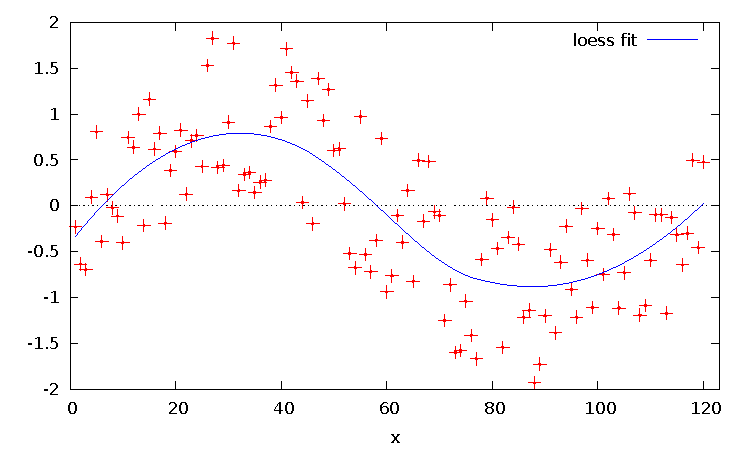
\includegraphics[scale=0.75]{figures/loess-sine}
  \caption{Loess: retrieving a sine wave}
  \label{fig:loess-sine}
\end{figure}

\section{The Nadaraya--Watson estimator}
\label{sec:nadarwat}

The Nadaraya--Watson nonparametric estimator \citep{nadaraya64,
  watson64} is an estimator for the conditional mean of a variable
$Y$, available in a sample of size $n$, for a given value of a
conditioning variable $X$, and is defined as
\[
  m(X) = \frac{ \sum_{j=1}^{n} y_j \cdot K_h(X - x_j)} {\sum_{j=1}^{n} K_h(X - x_j)}
\]
where $K_h(\cdot)$ is the so-called \emph{kernel function}, which is
usually some simple transform of a density function that depends on a
scalar called the \emph{bandwidth}. The one gretl uses is given
by
\[
  K_h(x) = \exp\left(-\frac{x^2}{2h}\right)
\]
for $|x| < \tau$ and zero otherwise. The scalar $\tau$ is used to
prevent numerical problems when the kernel function is evaluated too
far away from zero and is called the trim parameter.

\begin{script}[htbp]
  \caption{Nadaraya--Watson example}
  \label{scr:nadarwat-ex}
\begin{scode}
# Nonparametric regression example: husband's age on wife's age
open mroz87.gdt

# initial value for the bandwidth
scalar h = $nobs^(-0.2)
# three increasingly smoother estimates
series m0 = nadarwat(HA, WA, h)
series m1 = nadarwat(HA, WA, h * 5)
series m2 = nadarwat(HA, WA, h * 10)

# produce the graph
dataset sortby WA
gnuplot m0 m1 m2 HA WA --output=display --with-lines
\end{scode}
%$
\end{script}

\begin{figure}[htbp]
  \centering
  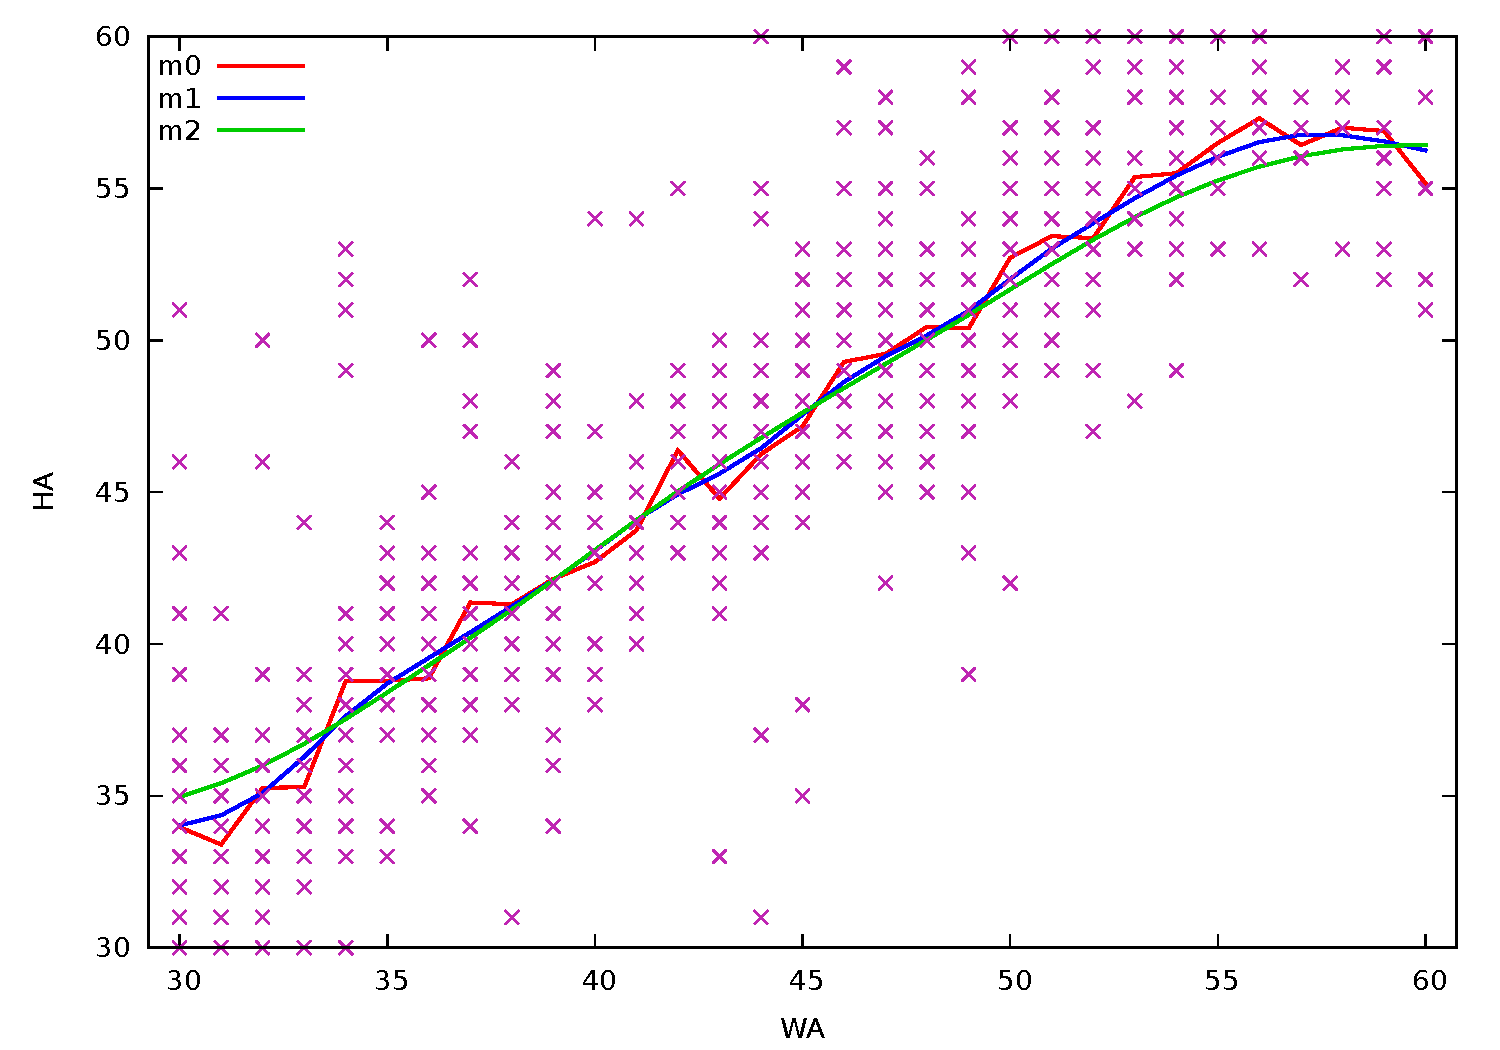
\includegraphics[scale=0.5]{figures/nadarwat-ex}
  \caption{Nadaraya--Watson example for several choices of the bandwidth parameter}
  \label{fig:nadarwat-ex}
\end{figure}

Example~\ref{scr:nadarwat-ex} produces the graph shown in
Figure~\ref{fig:nadarwat-ex} (after some slight editing).

The choice of the bandwidth is up to the user: larger values of $h$
lead to a smoother $m(\cdot)$ function; smaller values make the
$m(\cdot)$ function follow the $y_i$ values more closely, so that the
function appears more ``jagged''. In fact, as $h \to \infty$, $m(x_i)
\to \bar{Y}$; on the contrary, if $h \to 0$, observations for which
$x_i \ne X$ are not taken into account at all when computing $m(X)$.

Also, the statistical properties of $m(\cdot)$ vary with $h$: its
variance can be shown to be decreasing in $h$, while its squared bias
is increasing in $h$.  It can be shown that choosing $h \sim n^{-1/5}$
minimizes the RMSE, so that value is customarily taken as a reference
point.

Note that the kernel function has its tails ``trimmed''. The scalar
$\tau$, which controls the level at which trimming occurs is set by
default at $4 \cdot h$; this setting, however, may be changed via the
\cmd{set} command. For example,
\begin{code}
  set nadarwat_trim 10
\end{code}
sets $\tau = 10 \cdot h$. This may at times produce more sensible
results in regions of $X$ with sparse support; however, you should be
aware that in those same cases machine precision (division by
numerical zero) may render your results spurious. The default is
relatively safe, but experimenting with larger values may be a sensible
strategy in some cases.

A common variant of the Nadaraya--Watson estimator is the so-called
``leave-one-out'' estimator: this is a variant of the estimator that
does not use the $i$-th observation for evaluating $m(x_i)$. This
makes the estimator more robust numerically and its usage is often
advised for inference purposes.  In formulae, the leave-one-out
estimator is
\[
m(x_i) = \frac{ \sum_{j \ne i} y_j \cdot K_h(x_i -
  x_j)} {\sum_{j \ne i} K_h(x_i - x_j)}
\]
In order to have gretl compute the leave-one-out estimator, just
reverse the sign of $h$: if we changed example \ref{scr:nadarwat-ex} by
substituting
\begin{code}
  scalar h = $nobs^(-0.2)
\end{code}
with
\begin{code}
  scalar h = -($nobs^(-0.2))
\end{code}
the rest of the example would have stayed unchanged, the only
difference being the usage of the leave-one-out estimator.

Although $X$ could be, in principle, any value, in the typical usage
of this estimator you want to compute $m(X)$ for $X$ equal to one or
more values actually observed in your sample, that is $m(x_i)$. If you
need a point estimate of $m(X)$ for some value of $X$ which is not
present among the valid observations of your dependent variable, you
may want to add some ``fake'' observations to your dataset in which
$y$ is missing and $x$ contains the values you want $m(x)$ evaluated
at. For example, the following script evaluates $m(x)$ at regular
intervals between -2.0 and 2.0:

\begin{code}
nulldata 120
set seed 120496

# first part of the sample: actual data
smpl 1 100
x = normal()
y = x^2 + sin(x) + normal()

# second part of the sample: fake x data
smpl 101 120
x = (obs-110) / 5

# compute the Nadaraya-Watson estimate
# with bandwidth equal to 0.4 (note that
# 100^(-0.2) = 0.398)
smpl full
m = nadarwat(y, x, 0.4)

# show m(x) for the fake x values only
smpl 101 120
print x m -o
\end{code}

and running it produces
\begin{code}
               x            m

101         -1.8     1.165934
102         -1.6     0.730221
103         -1.4     0.314705
104         -1.2     0.026057
105         -1.0    -0.131999
106         -0.8    -0.215445
107         -0.6    -0.269257
108         -0.4    -0.304451
109         -0.2    -0.306448
110          0.0    -0.238766
111          0.2    -0.038837
112          0.4     0.354660
113          0.6     0.908178
114          0.8     1.485178
115          1.0     2.000003
116          1.2     2.460100
117          1.4     2.905176
118          1.6     3.380874
119          1.8     3.927682
120          2.0     4.538364
\end{code}

%%% Local Variables: 
%%% mode: latex
%%% TeX-master: "gretl-guide"
%%% End: 


\part{Technical details}

\chapter{Gretl and \TeX}
\label{gretltex}


\section{Introduction}
\label{tex-intro}

\TeX\ --- initially developed by Donald Knuth of Stanford University
and since enhanced by hundreds of contributors around the world --- is
the gold standard of scientific typesetting.  Gretl provides
various hooks that enable you to preview and print econometric results
using the \TeX\ engine, and to save output in a form suitable for
further processing with \TeX.

This chapter explains the finer points of gretl's \TeX-related
functionality.  The next section describes the relevant menu items;
section~\ref{tex-tune} discusses ways of fine-tuning \TeX\ output; and
section~\ref{tex-install} gives some pointers on installing (and
learning) \TeX\ if you do not already have it on your computer.  (Just
to be clear: \TeX\ is not included with the gretl distribution;
it is a separate package, including several programs and a large
number of supporting files.)

Before proceeding, however, it may be useful to set out briefly the
stages of production of a final document using \TeX.  For the most
part you don't have to worry about these details, since, in regard to
previewing at any rate, gretl handles them for you.  But having
some grasp of what is going on behind the scences will enable you to
understand your options better.

The first step is the creation of a plain text ``source'' file,
containing the text or mathematics to be typset, interspersed with
mark-up that defines how it should be formatted.  The second step is
to run the source through a processing engine that does the actual
formatting.  Typically this is either:
\begin{itemize}
\item a program called \app{latex} that generates so-called DVI
  (device-independent) output, or
\item (more commonly nowadays) a program called \app{pdflatex} that
  generates PDF output.\footnote{Experts will be aware of something
    called ``plain \TeX'', which is processed using the program
    \app{tex}.  The great majority of \TeX\ users, however, use the
    \LaTeX\ macros, initially developed by Leslie Lamport.
    gretl does not support plain \TeX.}
\end{itemize}

For previewing, one uses either a DVI viewer (typically \app{xdvi} on
GNU/Linux systems) or a PDF viewer (for example, Adobe's Acrobat
Reader or \app{xpdf}), depending on how the source was processed.  If
the DVI route is taken, there's then a third step to produce printable
output, typically using the program \app{dvips} to generate a
PostScript file.  If the PDF route is taken, the output is ready for
printing without any further processing.

On MS Windows and Mac OS X, gretl calls \app{pdflatex} to
process the source file, and expects the operating system to be able
to find the default viewer for PDF output; DVI is not supported.  On
GNU/Linux the default is also to produce PDF, but if you prefer the
DVI/PostScript route you can do the following: select the menu item
``Tools, Preferences, General'' then the ``Programs'' tab.  Find the
item titled ``Command to compile TeX files'', and set this to
\texttt{latex}.  In the same window, Make sure the commands to view
DVI and PostScript files are set to something appropriate for your
system.

\section{\TeX-related menu items}
\label{tex-menus}

\subsection{The model window}

The fullest \TeX\ support in gretl is found in the GUI model
window.  This has a menu item titled ``LaTeX'' with sub-items
``View'', ``Copy'', ``Save'' and ``Equation options'' (see
Figure~\ref{fig:latex-menu}).  

\begin{figure}[htbp]
  \caption{\LaTeX\ menu in model window}
  \label{fig:latex-menu}
  \begin{center}
    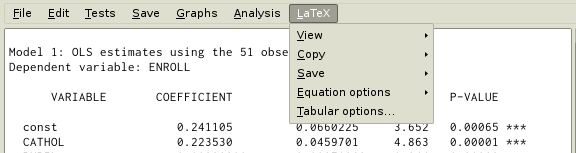
\includegraphics[scale=0.75]{figures/latex_menu}
  \end{center}
\end{figure}

The first three sub-items have branches titled ``Tabular'' and
``Equation''.  By ``Tabular'' we mean that the model is represented in
the form of a table; this is the fullest and most explicit
presentation of the results.  See Table~\ref{tab:mod1} for an example;
this was pasted into the manual after using the ``Copy, Tabular'' item
in gretl (a few lines were edited out for brevity).

\begin{table}[htbp]
\caption{Example of \LaTeX\ tabular output}
\label{tab:mod1}
\begin{center}

Model 1: OLS estimates using the 51 observations 1--51\\
Dependent variable: ENROLL\\

\vspace{1em}

\begin{tabular*}{.8\textwidth}{@{\extracolsep{\fill}}
l% col 1: varname
  D{.}{.}{-1}% col 2: coeff
    D{.}{.}{-1}% col 3: sderr
      D{.}{.}{-1}% col 4: t-stat
        D{.}{.}{4}}% col 5: p-value (or slope)
Variable &
  \multicolumn{1}{c}{Coefficient} &
    \multicolumn{1}{c}{Std.\ Error} &
      \multicolumn{1}{c}{$t$-statistic} &
        \multicolumn{1}{c}{p-value} \\[1ex]
const &
  0.241105 &
    0.0660225 &
      3.6519 &
        0.0007 \\
CATHOL &
  0.223530 &
    0.0459701 &
      4.8625 &
        0.0000 \\
PUPIL &
  -0.00338200 &
    0.00271962 &
      -1.2436 &
        0.2198 \\
WHITE &
  -0.152643 &
    0.0407064 &
      -3.7499 &
        0.0005 \\
\end{tabular*}

\vspace{1em}

\begin{tabular}{lD{.}{.}{-1}}
Mean of dependent variable & 0.0955686 \\
 S.D. of dependent variable & 0.0522150 \\
Sum of squared residuals & 0.0709594 \\
Standard error of residuals ($\hat{\sigma}$) & 0.0388558 \\
Unadjusted $R^2$ & 0.479466 \\
Adjusted $\bar{R}^2$ & 0.446241 \\
$F(3, 47)$ & 14.4306 \\
\end{tabular}
\end{center}
\end{table}

The ``Equation'' option is fairly self-explanatory---the results are
written across the page in equation format, as below:

%%% the following needs the amsmath LaTeX package

\begin{gather}
\widehat{\rm ENROLL} = 
\underset{(0.066022)}{0.241105}
+\underset{(0.04597)}{0.223530}\,\mbox{CATHOL}
-\underset{(0.0027196)}{0.00338200}\,\mbox{PUPIL}
-\underset{(0.040706)}{0.152643}\,\mbox{WHITE}
 \notag \\
T = 51 \quad \bar{R}^2 = 0.4462 \quad F(3,47) = 14.431 \quad \hat{\sigma} = 0.038856\notag \\
\centerline{(standard errors in parentheses)} \notag
\end{gather}

The distinction between the ``Copy'' and ``Save'' options (for both
tabular and equation) is twofold.  First, ``Copy'' puts the \TeX\
source on the clipboard while with ``Save'' you are prompted for the
name of a file into which the source should be saved.  Second, with
``Copy'' the material is copied as a ``fragment'' while with ``Save''
it is written as a complete file.  The point is that a well-formed
\TeX\ source file must have a header that defines the
\texttt{documentclass} (article, report, book or whatever) and tags
that say \verb|\begin{document}| and \verb|\end{document}|.  This
material is included when you do ``Save'' but not when you do
``Copy'', since in the latter case the expectation is that you will
paste the data into an existing \TeX\ source file that already has the
relevant apparatus in place.

The items under ``Equation options'' should be self-explanatory: when
printing the model in equation form, do you want standard errors or
$t$-ratios displayed in parentheses under the parameter estimates?
The default is to show standard errors; if you want $t$-ratios, select
that item.  

\subsection{Other windows}

Several other sorts of output windows also have \TeX\ preview, copy
and save enabled.  In the case of windows having a graphical toolbar,
look for the \TeX\ button.  Figure~\ref{fig:tex-icon} shows this icon
(second from the right on the toolbar) along with the dialog that
appears when you press the button.

\begin{figure}[htbp]
  \caption{\TeX\ icon and dialog}
  \label{fig:tex-icon}
    \begin{center}
      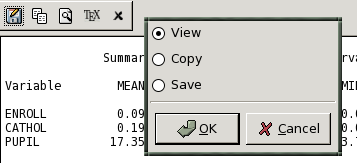
\includegraphics[scale=0.75]{figures/texdialog} 
    \end{center}
\end{figure}

One aspect of gretl's \TeX\ support that is likely to be
particularly useful for publication purposes is the ability to produce
a typeset version of the ``model table'' (see
section~\ref{model-table}).  An example of this is shown in
Table~\ref{tab:modeltab}.

\begin{table}[htbp]
\caption{Example of model table output}
\label{tab:modeltab}
\begin{center}
OLS estimates\\
Dependent variable: ENROLL \\
\vspace{1em}

\begin{tabular}{lccc}
 & Model 1  & Model 2  & Model 3 \\  [6pt] 
const & $\,\,$0.2907$^{**}$ & $\,\,$0.2411$^{**}$ & 0.08557 \\
& \footnotesize{(0.07853)} & \footnotesize{(0.06602)} & \footnotesize{(0.05794)} \\ [4pt] 
CATHOL & $\,\,$0.2216$^{**}$ & $\,\,$0.2235$^{**}$ & $\,\,$0.2065$^{**}$ \\
& \footnotesize{(0.04584)} & \footnotesize{(0.04597)} & \footnotesize{(0.05160)} \\ [4pt] 
PUPIL & $-$0.003035 & $-$0.003382 & $-$0.001697 \\
& \footnotesize{(0.002727)} & \footnotesize{(0.002720)} & \footnotesize{(0.003025)} \\ [4pt] 
WHITE & $\,\,$$-$0.1482$^{**}$ & $\,\,$$-$0.1526$^{**}$ & \\
& \footnotesize{(0.04074)} & \footnotesize{(0.04071)} & \\ [4pt] 
ADMEXP & $-$0.1551 & & \\
& \footnotesize{(0.1342)} & & \\ [4pt] 
$n$ & 51 & 51 & 51 \\
$\bar R^2$ & 0.4502 & 0.4462 & 0.2956 \\
$\ell$ & 96.09 & 95.36 & 88.69 \\
\end{tabular}

\vspace{1em}
Standard errors in parentheses\\
{}* indicates significance at the 10 percent level\\
{}** indicates significance at the 5 percent level\\
\end{center}
\end{table}


\section{Fine-tuning typeset output}
\label{tex-tune}

There are three aspects to this: adjusting the appearance of the
output produced by gretl in \LaTeX\ preview mode; adjusting the
formatting of gretl's tabular output for models when using the
\texttt{tabprint} command; and incorporating gretl's output into
your own \TeX\ files.


\subsection{Previewing in the GUI}

As regards \emph{preview mode}, you can control the appearance of
gretl's output using a file named \verb+gretlpre.tex+, which
should be placed in your gretl user directory (see the \GCR).
If such a file is found, its contents will be used as the ``preamble''
to the \TeX\ source.  The default value of the preamble is as follows:
    
\begin{code}
\documentclass[11pt]{article}
\usepackage[utf8]{inputenc}
\usepackage{amsmath}
\usepackage{dcolumn,longtable}
\begin{document}
\thispagestyle{empty}
\end{code}

Note that the \verb+amsmath+ and \verb+dcolumn+ packages are required.
(For some sorts of output the \verb+longtable+ package is also
needed.)  Beyond that you can, for instance, change the type size or
the font by altering the \texttt{documentclass} declaration or
including an alternative font package.

In addition, if you wish to typeset gretl output in more than
one language, you can set up per-language preamble files.  A
``localized'' preamble file is identified by a name of the form
\verb|gretlpre_xx.tex|, where \texttt{xx} is replaced by the first two
letters of the current setting of the \texttt{LANG} environment
variable.  For example, if you are running the program in Polish,
using \verb|LANG=pl_PL|, then gretl will do the following when
writing the preamble for a \TeX\ source file.

\begin{enumerate}
\item Look for a file named \verb|gretlpre_pl.tex| in the gretl
  user directory.  If this is not found, then
\item look for a file named \verb|gretlpre.tex| in the gretl
  user directory.  If this is not found, then
\item use the default preamble.
\end{enumerate}

Conversely, suppose you usually run gretl in a language other
than English, and have a suitable \verb|gretlpre.tex| file in place
for your native language.  If on some occasions you want to produce
\TeX\ output in English, then you could create an additional
file \verb|gretlpre_en.tex|: this file will be used for the preamble
when gretl is run with a language setting of, say,
\verb|en_US|.  


\subsection{Command-line options}

After estimating a model via a script---or interactively via the gretl
console or using the command-line program \app{gretlcli}---you can use
the commands \texttt{tabprint} or \texttt{eqnprint} to print the model
to file in tabular format or equation format respectively.  These
options are explained in the \GCR{}.

If you wish alter the appearance of gretl's tabular output for
models in the context of the \texttt{tabprint} command, you can
specify a custom row format using the \option{format} flag.  The
format string must be enclosed in double quotes and must be tied to
the flag with an equals sign.  The pattern for the format string is as
follows.  There are four fields, representing the coefficient,
standard error, $t$-ratio and p-value respectively.  These fields
should be separated by vertical bars; they may contain a
\texttt{printf}-type specification for the formatting of the numeric
value in question, or may be left blank to suppress the printing of
that column (subject to the constraint that you can't leave all the
columns blank).  Here are a few examples:

\begin{code}
--format="%.4f|%.4f|%.4f|%.4f"
--format="%.4f|%.4f|%.3f|"
--format="%.5f|%.4f||%.4f"
--format="%.8g|%.8g||%.4f"
\end{code}

The first of these specifications prints the values in all columns
using 4 decimal places.  The second suppresses the p-value and prints
the $t$-ratio to 3 places.  The third omits the $t$-ratio.  The last
one again omits the $t$, and prints both coefficient and standard
error to 8 significant figures.

Once you set a custom format in this way, it is remembered and used
for the duration of the gretl session.  To revert to the default
formatting you can use the special variant \verb|--format=default|.


\subsection{Further editing}

Once you have pasted gretl's \TeX\ output into your own
document, or saved it to file and opened it in an editor, you can of
course modify the material in any wish you wish.  In some cases,
machine-generated \TeX\ is hard to understand, but gretl's
output is intended to be human-readable and -editable.  In addition,
it does not use any non-standard style packages.  Besides the standard
\LaTeX\ document classes, the only files needed are, as noted above,
the \verb+amsmath+, \verb+dcolumn+ and \verb+longtable+ packages.
These should be included in any reasonably full \TeX\ implementation.


\section{Installing and learning \TeX}
\label{tex-install}

This is not the place for a detailed exposition of these matters, but
here are a few pointers.  

So far as we know, every GNU/Linux distribution has a package or set
of packages for \TeX, and in fact these are likely to be installed by
default.  Check the documentation for your distribution.  For MS
Windows, several packaged versions of \TeX\ are available: one of the
most popular is MiK\TeX\, at \url{http://www.miktex.org/}.  For Mac OS
X a nice implementation is i\TeX{}Mac, at
\url{http://itexmac.sourceforge.net/}.  An essential starting point for
online \TeX\ resources is the Comprehensive
\TeX\ Archive Network (CTAN) at \url{http://www.ctan.org/}.

As for learning \TeX, many useful resources are available both online
and in print.  Among online guides, Tony Roberts' ``\LaTeX: from quick
and dirty to style and finesse'' is very helpful, at

\url{http://www.sci.usq.edu.au/staff/robertsa/LaTeX/latexintro.html}

An excellent source for advanced material is \emph{The \LaTeX\
  Companion} \citep{goossens04}.


%%% Local Variables: 
%%% mode: latex
%%% TeX-master: "gretl-guide"
%%% End: 

\chapter{Gretl and R}
\label{chap:gretlR}

\section{Introduction}
\label{R-intro}

\app{R} is, by far, the largest free statistical
project.\footnote{\app{R}'s homepage is at
  \url{http://www.r-project.org/}.} Like \app{gretl}, it is a GNU
project and the two have a lot in common; however, \app{gretl}'s
approach focuses on ease of use much more than \app{R}, which instead
aims to encompass the widest possible range of statistical procedures.

As is natural in the free software ecosystem, we don't view ourselves
as competitors to \app{R},\footnote{OK, who are we kidding? But it's
  \emph{friendly} competition!} but rather as projects sharing a common
goal who should support each other whenever possible. For this reason,
\app{gretl} provides a way to interact with \app{R} and thus enable
users to pool the capabilities of the two packages.

In this chapter, we will explain how to exploit \app{R}'s power from
within \app{gretl}. We assume that the reader has a working
installation of \app{R} available and a basic grasp of \app{R}'s
syntax.\footnote{The main reference for \app{R} documentation is
  \url{http://cran.r-project.org/manuals.html}.  In addition, \app{R}
  tutorials abound on the Net; as always, Google is your friend.}

Despite several valiant attempts, no graphical shell has gained wide
acceptance in the \app{R} community: by and large, the standard method
of working with \app{R} is by writing scripts, or by typing commands
at the \app{R} prompt, much in the same way as one would write
\app{gretl} scripts or work with the \app{gretl} console. In this
chapter, the focus will be on the methods available to execute \app{R}
commands without leaving \app{gretl}.

\section{Starting an interactive \app{R} session}
\label{sec:R-interactive}

The easiest way to use \app{R} from \app{gretl} is in interactive
mode.  Once you have your data loaded in \app{gretl}, you can select
the menu item ``Tools, Start GNU R'' and an interactive \app{R}
session will be started, with your dataset automatically pre-loaded.

\subsection{A simple example: OLS on cross-section data}
\label{sec:R-ols-ex}

For this example we use Ramanathan's dataset \texttt{data4-1}, one of
the sample files supplied with \app{gretl}.  We first run, in
\app{gretl}, an OLS regression of \texttt{price} on \texttt{sqft},
\texttt{bedrms} and \texttt{baths}.  The basic results are shown in
Table \ref{tab:data4-1-gretlOLS}.

\begin{table}[htbp]
\caption{OLS house price regression via \app{gretl}}
\label{tab:data4-1-gretlOLS}
\begin{center}

\begin{tabular*}{0.75\textwidth}{@{\extracolsep{\fill}}
l% col 1: varname
  D{.}{.}{-1}% col 2: coeff
    D{.}{.}{-1}% col 3: sderr
      D{.}{.}{-1}% col 4: t-stat
        D{.}{.}{4}}% col 5: p-value (or slope)
Variable &
  \multicolumn{1}{c}{Coefficient} &
    \multicolumn{1}{c}{Std.\ Error} &
      \multicolumn{1}{c}{$t$-statistic} &
        \multicolumn{1}{c}{p-value} \\[1ex]
const &
  129.062 &
    88.3033 &
      1.4616 &
        0.1746 \\
sqft &
  0.154800 &
    0.0319404 &
      4.8465 &
        0.0007 \\
bedrms &
  -21.587 &
    27.0293 &
      -0.7987 &
        0.4430 \\
baths &
  -12.192 &
    43.2500 &
      -0.2819 &
        0.7838 \\
\end{tabular*}
\end{center}
\end{table}

We will now replicate the above results using \app{R}. Select 
the menu item ``Tools, Start GNU R''. A window similar to the one
shown in figure \ref{fig:Rwind1} should appear.

\begin{figure}[htbp]
  \centering
  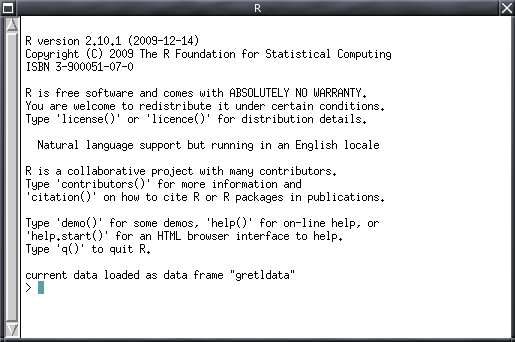
\includegraphics[scale=0.7]{figures/Rwindow-1}
  \caption{\app{R} window}
  \label{fig:Rwind1}
\end{figure}

The actual look of the \app{R} window may be somewhat different from
what you see in Figure~\ref{fig:Rwind1} (especially for Windows
users), but this is immaterial. The important point is that you have a
window where you can type commands to \app{R}. If the above procedure
doesn't work and no \app{R} window opens, it means that \app{gretl}
was unable to launch \app{R}.  You should ensure that \app{R} is
installed and working on your system and that \app{gretl} knows where
it is. The relevant settings can be found by selecting the ``Tools,
Preferences, General'' menu entry, under the ``Programs'' tab.

Assuming \app{R} was launched successfully, you will see notification
that the data from gretl are available.  In the background,
\app{gretl} has arranged for two \app{R} commands to be executed, one
to load the \app{gretl} dataset in the form of a \emph{data frame}
(one of several forms in which \app{R} can store data) and one to
\emph{attach} the data so that the variable names defined in the
\app{gretl} workspace are available as valid identifiers within
\app{R}.

In order to replicate \app{gretl}'s OLS estimation, go into the \app{R}
window and type at the prompt
\begin{code}
  model <- lm(price ~ sqft + bedrms + baths)
  summary(model)
\end{code}

\begin{figure}[htbp]
  \centering
  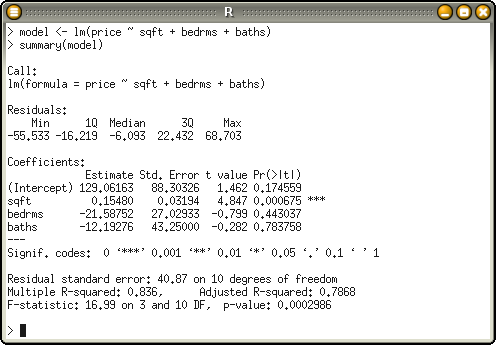
\includegraphics[scale=0.7]{figures/Rwindow-2}
  \caption{OLS regression on house prices via \app{R}}
  \label{fig:Rwind2}
\end{figure}

You should see something similar to Figure~\ref{fig:Rwind2}. Surprise
--- the estimates coincide! To get out, just close the \app{R} window
or type \verb|q()| at the \app{R} prompt.

\subsection{Time series data}
\label{sec:R-ols-arma}

We now turn to an example which uses time series data: we
will compare \app{gretl}'s and \app{R}'s estimates of Box and Jenkins'
immortal ``airline'' model. The data are contained in the \texttt{bjg}
sample dataset. The following \app{gretl} code
\begin{code}
open bjg
arima 0 1 1 ; 0 1 1 ; lg --nc
\end{code}
produces the estimates shown in Table \ref{tab:airline-gretl}.

\begin{table}[htbp]
\caption{Airline model from Box and Jenkins (1976) --- selected
  portion of \app{gretl}'s estimates}
\label{tab:airline-gretl}
\begin{center}

\begin{tabular*}{0.75\textwidth}{@{\extracolsep{\fill}}
l% col 1: varname
  D{.}{.}{-1}% col 2: coeff
    D{.}{.}{-1}% col 3: sderr
      D{.}{.}{-1}% col 4: t-stat
        D{.}{.}{4}}% col 5: p-value (or slope)
Variable &
  \multicolumn{1}{c}{Coefficient} &
    \multicolumn{1}{c}{Std.\ Error} &
      \multicolumn{1}{c}{$t$-statistic} &
        \multicolumn{1}{c}{p-value} \\[1ex]
$\theta_{1}$ &
  -0.401824 &
    0.0896421 &
      -4.4825 &
        0.0000 \\
$\Theta_{1}$ &
  -0.556936 &
    0.0731044 &
      -7.6184 &
        0.0000 \\
\end{tabular*}

\begin{tabular}{lD{.}{.}{-1}}
Variance of innovations & 0.00134810 \\
Log-likelihood & 244.696 \\
Akaike information criterion & -483.39 
\end{tabular}
\end{center}
\end{table}

If we now open an \app{R} session as described in the previous
subsection, the data-passing mechanism is slightly different.  Since
our data were defined in \app{gretl} as time series, we use an \app{R}
\emph{time-series} object (\emph{ts} for short) for the transfer.  In
this way we can retain in \app{R} useful information such as the
periodicity of the data and the sample limits.  The downside is that
the names of individual series, as defined in \app{gretl}, are not
valid identifiers. In order to extract the variable \texttt{lg}, one
needs to use the syntax \verb|lg <- gretldata[, "lg"]|.

ARIMA estimation can be carried out by issuing the following two
\app{R} commands:
\begin{code}
lg <- gretldata[, "lg"]
arima(lg, c(0,1,1), seasonal=c(0,1,1))
\end{code}

which yield

\begin{code}
Coefficients:
          ma1     sma1
      -0.4018  -0.5569
s.e.   0.0896   0.0731

sigma^2 estimated as 0.001348:  log likelihood = 244.7,  aic = -483.4
\end{code}

Happily, the estimates again coincide.

\section{Running an \app{R} script}
\label{sec:R-scripts}

Opening an \app{R} window and keying in commands is a convenient
method when the job is small. In some cases, however, it would be
preferable to have \app{R} execute a script prepared in advance. 
One way to do this is via the \texttt{source()} command in
\app{R}.  Alternatively, \app{gretl} offers the facility to edit an
\app{R} script and run it, having the current dataset pre-loaded
automatically. This feature can be accessed via the ``File, Script
Files'' menu entry.  By selecting ``User file'', one can load a
pre-existing \app{R} script; if you want to create a new script
instead, select the ``New script, R script'' menu entry.

\begin{figure}[htbp]
  \centering
  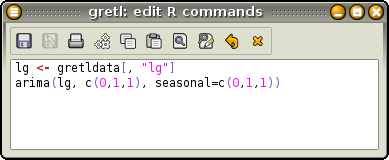
\includegraphics[scale=0.7]{figures/R-edit1}
  \caption{Editing window for \app{R} scripts}
  \label{fig:R-edit1}
\end{figure}
In either case, you are presented with a window very similar to
the editor window used for ordinary \app{gretl} scripts, as in
Figure~\ref{fig:R-edit1}.

There are two main differences.  First, you get syntax highlighting for
\app{R}'s syntax instead of \app{gretl}'s. Second, clicking on the
Execute button (the gears icon), launches an instance of \app{R} in
which your commands are executed.  Before \app{R} is actually run, you
are asked if you want to run \app{R} interactively or not (see
Figure~\ref{fig:R-exec-mode}).

\begin{figure}[htbp]
  \centering
  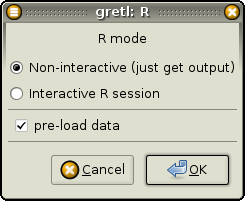
\includegraphics[scale=0.7]{figures/R-exec-mode}
  \caption{Editing window for \app{R} scripts}
  \label{fig:R-exec-mode}
\end{figure}

An interactive run opens an \app{R} instance similar to the one seen
in the previous section: your data will be pre-loaded (if the
``pre-load data'' box is checked) and your commands will
be executed. Once this is done, you will find yourself at the \app{R}
prompt, where you can enter more commands.

A non-interactive run, on the other hand, will execute your script,
collect the output from \app{R} and present it to you in an output
window; \app{R} will be run in the background. If, for example, the
script in Figure~\ref{fig:R-edit1} is run non-interactively, a window
similar to Figure~\ref{fig:R-output1} will appear.

\begin{figure}[htbp]
  \centering
  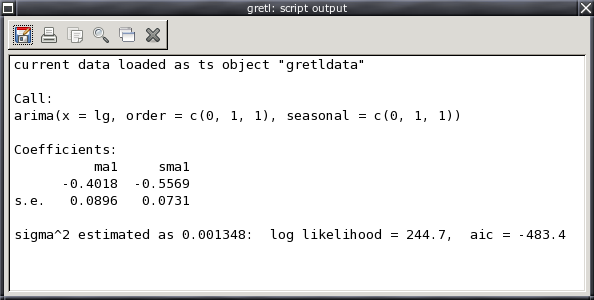
\includegraphics[scale=0.7]{figures/R-output1}
  \caption{Output from a non-interactive \app{R} run}
  \label{fig:R-output1}
\end{figure}

\section{Taking stuff back and forth}
\label{sec:R-passing-data}

As regards the passing of data between the two programs, so far we
have only considered passing series from \app{gretl} to \app{R}. In
order to achieve a satisfactory degree of interoperability, more is
needed.  In the following sub-sections we see how matrices can be
exchanged, and how data can be passed from \app{R} back to
\app{gretl}.

\subsection{Passing matrices from \app{gretl} to \app{R}}

For passing matrices from \app{gretl} to \app{R}, you can use the
\texttt{mwrite} matrix function described in section
\ref{sec:matrix-csv}. For example, the following \app{gretl} code
fragment generates the matrix 
\[ 
A = \left[
  \begin{array}{ccc}
    3 &  7 &  11 \\ 
    4 &  8 &  12 \\ 
    5 &  9 &  13 \\ 
    6 & 10 &  14 
  \end{array}
\right]
\] 
and stores it into the file \texttt{mymatfile.mat}.
\begin{code}
  matrix A = mshape(seq(3,14),4,3)
  err = mwrite(A, "mymatfile.mat")
\end{code}
In order to retrieve this matrix from \app{R}, all you have to do is
\begin{code}
  A <- as.matrix(read.table("mymatfile.mat", skip=1))
\end{code}

Although in principle you can give your matrix file any valid
filename, a couple of conventions may prove useful. First, you may
want to use an informative file suffix such as ``\texttt{.mat}'', but
this is a matter of taste. More importantly, the exact location of the
file created by \texttt{mwrite} could be an issue. By default, if no
path is specified in the file name, \app{gretl} stores matrix files in
the current work directory. However, it may be wise for the purpose at
hand to use the directory in which \app{gretl} stores all its
temporary files, whose name is stored in the built-in string
\texttt{dotdir} (see section~\ref{sec:named-strings}). The value of
this string is automatically passed to \app{R} as the string variable
\texttt{gretl.dotdir}, so the above example may be rewritten more
cleanly as

\app{Gretl} side:
\begin{code}
  matrix A = mshape(seq(3,14),4,3)
  err = mwrite(A, "@dotdir/mymatfile.mat")
\end{code}
\app{R} side:
\begin{code}
  fname <- paste(gretl.dotdir, "mymatfile.mat", sep="")
  A <- as.matrix(read.table(fname, skip=1))
\end{code}

\subsection{Passing data from \app{R} to \app{gretl}}
\label{sec:Rpassing-data}

For passing data in the opposite direction, \app{gretl} defines a
special function that can be used in the \app{R} environment. An
\app{R} object will be written as a temporary file in \app{gretl}'s
\texttt{dotdir} directory, from where it can be easily retrieved from
within \app{gretl}.

The name of this function is \texttt{gretl.export()}, and it accepts
one argument, the object to be exported. At present, the objects that
can be exported with this method are matrices, data frames and
time-series objects. The function creates a text file, with the same
name as the exported object, in \app{gretl}'s temporary
directory. Data frames and time-series objects are stored as CSV
files, and can be retrieved by using \app{gretl}'s \texttt{append}
command.  Matrices are stored in a special text format that is
understood by \app{gretl} (see section~\ref{sec:matrix-csv}); the file
suffix is in this case \texttt{.mat}, and to read the matrix in
\app{gretl} you must use the \texttt{mread()} function.

As an example, we take the airline data and use them to estimate a
structural time series model \`a la \cite{harvey89}. The model we will 
use is the \emph{Basic Structural Model} (BSM), in which a time series
is decomposed into three terms:
\[
  y_t = \mu_t + \gamma_t + \varepsilon_t
\]
where $\mu_t$ is a trend component, $\gamma_t$ is a seasonal component
and $\varepsilon_t$ is a noise term. In turn, the following is assumed
to hold:
\begin{eqnarray*}
  \Delta \mu_t & = & \beta_{t-1} + \eta_t \\
  \Delta \beta_t & = & \zeta_t \\
  \Delta_s \gamma_t & = & \Delta \omega_t
\end{eqnarray*}
where $\Delta_s$ is the seasonal differencing operator, $(1-L^s)$, and
$\eta_t$, $\zeta_t$ and $\omega_t$ are mutually uncorrelated white
noise processes. The object of the analysis is to estimate the
variances of the noise components (which may be zero) and to recover
estimates of the latent processes $\mu_t$ (the ``level''), $\beta_t$
(the ``slope'') and $\gamma_t$.

\app{Gretl} does not provide (yet) a command for estimating this class
of models, so we will use \app{R}'s \texttt{StructTS} command and
import the results back into \app{gretl}. Once the \texttt{bjg}
dataset is loaded in \app{gretl}, we pass the data to \app{R} and execute
the following script:
\begin{code}
# extract the log series 
y <- gretldata[, "lg"]
# estimate the model
strmod <- StructTS(y)
# save the fitted components (smoothed)
compon <- as.ts(tsSmooth(strmod))
# save the estimated variances
vars <- as.matrix(strmod$coef)

# export into gretl's temp dir
gretl.export(compon)
gretl.export(vars)
\end{code}
%$

Running this script via \app{gretl} produces minimal output:
\begin{code}
current data loaded as ts object "gretldata"
wrote /home/cottrell/.gretl/compon.csv 
wrote /home/cottrell/.gretl/vars.mat 
\end{code}
However, we are now able to pull the results back into \app{gretl} by
executing the following commands, either from the console or by
creating a small script:\footnote{This example will work on Linux and
  presumably on OSX without modifications. On the Windows platform,
  you may have to substitute the ``\texttt{/}'' character with
  ``$\backslash$''.}
\begin{code}
append @dotdir/compon.csv
vars = mread("@dotdir/vars.mat")
\end{code}
The first command reads the estimated time-series components from a
CSV file, which is the format that the passing mechanism employs for
series. The matrix \texttt{vars} is read from the file
\texttt{vars.mat}.

\begin{figure}[htbp]
  \centering
  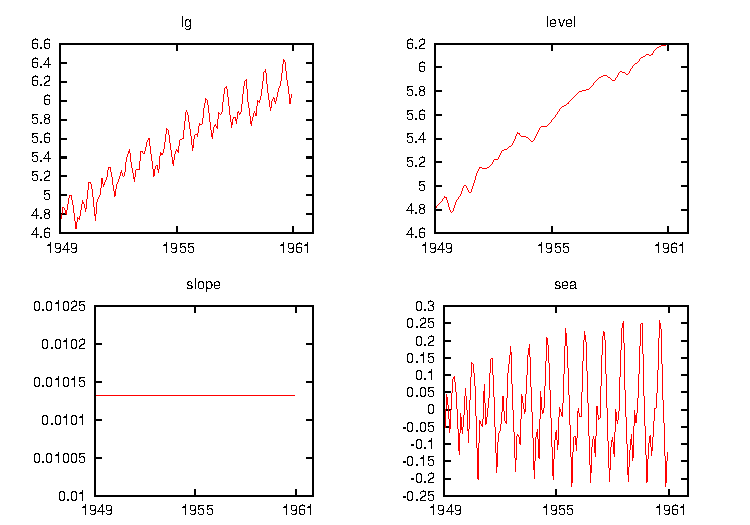
\includegraphics{figures/BSM-output}
  \caption{Estimated components from BSM}
  \label{fig:BSM-output}
\end{figure}

After the above commands have been executed, three new series will
have appeared in the \app{gretl} workspace, namely the estimates of
the three components; by plotting them together with the original
data, you should get a graph similar to
Figure~\ref{fig:BSM-output}. The estimates of the variances can be
seen by printing the \texttt{vars} matrix, as in

\begin{code}
? print vars
vars (4 x 1)

  0.00077185 
      0.0000 
   0.0013969 
      0.0000 
\end{code}

That is,
\begin{equation*}
  \hat{\sigma}^2_{\eta} = 0.00077185, \quad
  \hat{\sigma}^2_{\zeta} = 0, \quad
  \hat{\sigma}^2_{\omega} = 0.0013969, \quad
  \hat{\sigma}^2_{\varepsilon} = 0
\end{equation*}
Notice that, since $\hat{\sigma}^2_{\zeta} = 0$, the estimate for
$\beta_t$ is constant and the level component is simply a random walk
with a drift.

\section{Interacting with \app{R} from the command line}
\label{sec:foreign-command}

Up to this point we have spoken only of interaction with \app{R} via
the GUI program. In order to do the same from the command line
interface, \app{gretl} provides the \texttt{foreign} command. This
enables you to embed non-native commands within a \app{gretl}
script.

A ``foreign'' block takes the form
\begin{code}
foreign language=R [--send-data] [--quiet]
    ... R commands ...
end foreign
\end{code}
and achieves the same effect as submitting the enclosed \app{R}
commands via the GUI in the non-interactive mode (see
section~\ref{sec:R-scripts} above). The \option{send-data} option
arranges for auto-loading of the data present in the \app{gretl}
session.  The \option{quiet} option prevents the output from \app{R}
from being echoed in the \app{gretl} output.

\begin{script}[htbp]
  \caption{Estimation of the Basic Structural Model --- simple}
\begin{scode}
open bjg.gdt

foreign language=R --send-data
    y <- gretldata[, "lg"]
    strmod <- StructTS(y)
    compon <- as.ts(tsSmooth(strmod))
    vars <- as.matrix(strmod$coef)
            
    gretl.export(compon)
    gretl.export(vars)
end foreign

append @dotdir/compon.csv
rename level lg_level
rename slope lg_slope
rename sea lg_seas

vars = mread("@dotdir/vars.mat")
\end{scode}
\label{RStructTS-simple}
\end{script}
%$

Using this method, replicating the example in the previous subsection
is rather easy: basically, all it takes is encapsulating the content
of the \app{R} script in a \texttt{foreign}\ldots\texttt{end foreign}
block; see example \ref{RStructTS-simple}.

\begin{script}[htbp]
  \caption{Estimation of the Basic Structural Model --- via a function}
\begin{scode}
function list RStructTS(series myseries)

    smpl ok(myseries) --restrict
    sx = argname(myseries)

    foreign language=R --send-data --quiet
        @sx <- gretldata[, "myseries"]
        strmod <- StructTS(@sx)
        compon <- as.ts(tsSmooth(strmod))
        gretl.export(compon)
    end foreign

    append @dotdir/compon.csv
    rename level @sx_level
    rename slope @sx_slope
    rename sea @sx_seas

    list ret = @sx_level @sx_slope @sx_seas
    return ret
end function

# ------------ main -------------------------

open bjg.gdt
list X = RStructTS(lg)
\end{scode}

\label{RStructTS-func}
\end{script}

The above syntax, despite being already quite useful by itself, shows
its full power when it is used in conjunction with user-written
functions.  Example~\ref{RStructTS-func} shows how to define a
\app{gretl} function that calls \app{R} internally.

\section{Performance issues with \app{R}}
\label{sec:R-performance}

\app{R} is a large and complex program, which takes an appreciable
time to initialize itself.\footnote{About one third of a second on an
  Intel Core Duo machine of 2009 vintage.}  In interactive use this
not a significant problem, but if you have a \app{gretl} script that
calls \app{R} repeatedly the cumulated start-up costs can become
bothersome.  To get around this, \app{gretl} calls the \app{R} shared
library by preference; in this case the start-up cost is borne only
once, on the first invocation of \app{R} code from within \app{gretl}.

Support for the \app{R} shared library is built into the \app{gretl}
packages for MS Windows and OS X --- but the advantage is realized
only if the library is in fact available at run time.  If you are
building \app{gretl} yourself on Linux and wish to make use of the
\app{R} library, you should ensure (a) that \app{R} has been built
with the shared library enabled (specify \verb|--enable-R-shlib| when
configuring your build of \app{R}), and (b) that the \verb|pkg-config|
program is able to detect your \app{R} installation.  We do not link
to the \app{R} library at build time, rather we open it dynamically on
demand. The \app{gretl} GUI has an item under the
\textsf{Tools/Preferences} menu which enables you to select the
path to the library, if it is not detected automatically.  

If you have the \app{R} shared library installed but want to force
\app{gretl} to call the \app{R} executable instead, you can do
\begin{code}
set R_lib off
\end{code}

\section{Further use of the \app{R} library}
\label{sec:R-functions}

Besides improving performance, as noted above, use of the \app{R}
shared library makes possible a further refinement.  That is, you can
define functions in \app{R}, within a \texttt{foreign} block, then
call those functions later in your script much as if they were
\app{gretl} functions.  This is illustrated below.  
%
\begin{code}
set R_functions on
foreign language=R
  plus_one <- function(q) {
     z = q+1
     invisible(z)
  }
end foreign

scalar b=R.plus_one(2)
\end{code}
%
The \app{R} function \verb|plus_one| is obviously trivial in itself,
but the example shows a couple of points.  First, for this mechanism
to work you need to enable \verb|R_functions| via the \texttt{set}
command.  Second, to avoid collision with the \app{gretl} function
namespace, calls to functions defined in this way must be prefixed
with ``\texttt{R.}'', as in \verb|R.plus_one|.

Built-in \app{R} functions may also be called in this way, once
\verb|R_functions| is set \texttt{on}.  For example one can invoke
\app{R}'s \texttt{choose} function, which computes binomial
coefficients:
%
\begin{code}
set R_functions on
scalar b=R.choose(10,4)
\end{code}
%
Note, however, that the possibilities for use of built-in \app{R}
functions are limited; only functions whose arguments and return
values are sufficiently generic (basically scalars or matrices) will
work.

%%% Local Variables: 
%%% mode: latex
%%% TeX-master: "gretl-guide"
%%% End: 


\chapter{Gretl and Ox}
\label{chap:gretlOx}

\section{Introduction}
\label{Ox-intro}

\app{Ox}, written by Jurgen A. Doornik \citep[see][]{doornik07}, is
described by its author as ``an object-oriented statistical system. At
its core is a powerful matrix language, which is complemented by a
comprehensive statistical library. Among the special features of Ox
are its speed [and] well-designed syntax\dots{}.  Ox comes in two
versions: Ox Professional and Ox Console. Ox is available for Windows,
Linux, Mac (OS X), and several Unix platforms.''
(\url{www.doornik.com})

\app{Ox} is proprietary, closed-source software.  The command-line
version of the program is, however, available free of change for
academic users.  Quoting again from Doornik's website: ``The
Console (command line) versions may be used freely for academic
research and teaching purposes only\dots{}. The Ox syntax is public,
and, of course, you may do with your own Ox code whatever you wish.''
If you wish to use \app{Ox} in conjunction with gretl please
refer to \url{doornik.com} for further details on licensing.

As the reader will no doubt have noticed, most other software that
we discuss in this Guide is open-source and freely available for all
users.  We make an exception for \app{Ox} on the grounds that it is
indeed fast and well designed, and that its statistical
library---along with various add-on packages that are also
available---has exceptional coverage of cutting-edge techniques in
econometrics.  The gretl authors have used \app{Ox} for benchmarking
some of gretl's more advanced features such as dynamic panel models
and state space models.\footnote{For a review of \app{Ox}, see
  \cite{cribari-neto03} and for a (somewhat dated) comparison of
  \app{Ox} with other matrix-oriented packages such as \app{GAUSS},
  see \cite{steinhaus99}.}

\section{\app{Ox} support in gretl}
\label{sec:Ox-support}

The support offered for \app{Ox} in gretl is similar to that
offered for \app{R}, as discussed in chapter~\ref{chap:gretlR}.

\tip{To enable support for \app{Ox}, go to the
  Tools/Preferences/General menu item and look under the Programs
  tab. Find the entry for the path to the \texttt{oxl} executable,
  that is, the program that runs \app{Ox} files (on MS Windows it is
  called \texttt{oxl.exe}). Adjust the path if it's not already right
  for your system and you should be ready to go.}
  
With support enabled, you can open and edit \app{Ox} programs in the
gretl GUI.  Clicking the ``execute'' icon in the editor window
will send your code to \app{Ox} for execution.
Figures~\ref{fig:Oxedit} and Figure~\ref{fig:Oxout} show an \app{Ox}
program and part of its output.

\begin{figure}[htbp]
  \centering
  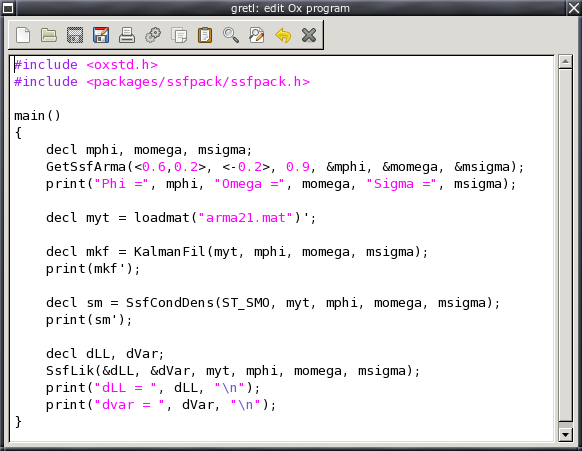
\includegraphics[scale=0.7]{figures/Oxedit}
  \caption{\app{Ox} editing window}
  \label{fig:Oxedit}
\end{figure}

\begin{figure}[htbp]
  \centering
  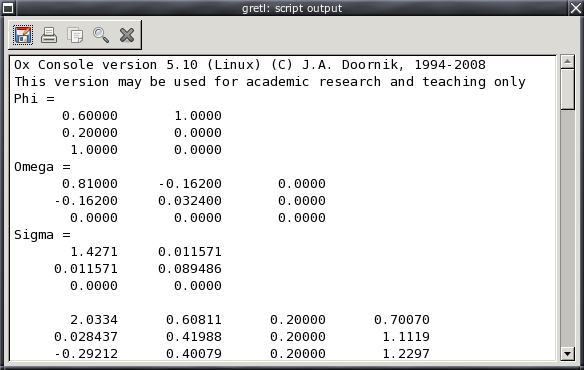
\includegraphics[scale=0.7]{figures/Oxout}
  \caption{Output from \app{Ox}}
  \label{fig:Oxout}
\end{figure}

In addition you can embed \app{Ox} code within a gretl script
using a \texttt{foreign} block, as described in connection with
\app{R}.  A trivial example, which simply prints the gretl data
matrix within \app{Ox}, is shown below:
%
\begin{code}
open data4-1
matrix m = { dataset }
mwrite(m, "gretl.mat", 1)

foreign language=Ox 
#include <oxstd.h>
main()
{
   decl gmat = gretl_loadmat("gretl.mat");
   print(gmat);
}
end foreign
\end{code}

The above example illustrates how a matrix can be passed from
gretl to \app{Ox}.  We use the \texttt{mwrite} function to write
a matrix into the user's ``dotdir'' (see
section~\ref{sec:named-strings}), then in \app{Ox} we use the function
\verb|gretl_loadmat| to retrieve the matrix.

How does \verb|gretl_loadmat| come to be defined?  When gretl
writes out the \app{Ox} program corresponding to your \texttt{foreign}
block it does two things in addition.  First, it writes a small
utility file named \verb|gretl_io.ox| into your dotdir.  This contains
a definition for \verb|gretl_loadmat| and also for the function
\verb|gretl_export| (see below).  Second, gretl interpolates
into your \app{Ox} code a line which includes this utility file (it is
inserted right after the inclusion of \texttt{oxstd.h}, which is
needed in all \app{Ox} programs).  Note that \verb|gretl_loadmat|
expects to find the named file in the user's dotdir.

\section{Illustration: replication of DPD model}
\label{sec:dpd-replication}

Example~\ref{Ox-DPD} shows a more ambitious case.  This script
replicates one of the dynamic panel data models in
\cite{arellano-bond91}, first using gretl and then using \app{Ox}; we
then check the relative differences between the parameter estimates
produced by the two programs (which turn out to be reassuringly
small).

Unlike the previous example, in this case we pass the dataset from
gretl to \app{Ox} as a CSV file in order to preserve the
variable names.  Note the use of the internal variable \verb|csv_na|
to get the right representation of missing values for use with
\app{Ox}---and also note that the \verb|--send-data| option for the
\texttt{foreign} command is not available in connection with Ox.

We get the parameter estimates back from \app{Ox} using
\verb|gretl_export| on the \app{Ox} side and \texttt{mread} on the
gretl side.  The \verb|gretl_export| function takes two
arguments, a matrix and a file name.  The file is written into the
user's dotdir, from where it can be picked up using \texttt{mread}.
The final portion of the output from Example~\ref{Ox-DPD} is shown
below:
%
\begin{code}
? matrix oxparm = mread("oxparm.mat", 1)
Generated matrix oxparm
? eval abs((parm - oxparm) ./ oxparm)
  1.4578e-13 
  3.5642e-13 
  5.0672e-15 
  1.6091e-13 
  8.9808e-15 
  2.0450e-14 
  1.0218e-13 
  2.1048e-13 
  9.5898e-15 
  1.8658e-14 
  2.1852e-14 
  2.9451e-13 
  1.9398e-13 
\end{code}

\begin{script}[htbp]
  \caption{Estimation of dynamic panel data model via gretl and \app{Ox}}
\begin{scode}
open abdata.gdt

# Take first differences of the independent variables
genr Dw = diff(w)
genr Dk = diff(k)
genr Dys = diff(ys)

# 1-step GMM estimation
arbond 2 ; n Dw Dw(-1) Dk Dys Dys(-1) 0 --time-dummies
matrix parm = $coeff

# Write CSV file for Ox
set csv_na .NaN
store @dotdir/abdata.csv

# Replicate using the Ox DPD package
foreign language=Ox
#include <oxstd.h>
#import <packages/dpd/dpd>

main ()
{
    decl dpd = new DPD();
    dpd.Load("@dotdir/abdata.csv"); 
    dpd.SetYear("YEAR");

    dpd.Select(Y_VAR, {"n", 0, 2});
    dpd.Select(X_VAR, {"w", 0, 1, "k", 0, 0, "ys", 0, 1});
    dpd.Select(I_VAR, {"w", 0, 1, "k", 0, 0, "ys", 0, 1});

    dpd.Gmm("n", 2, 99);  // GMM-type instrument
    dpd.SetDummies(D_CONSTANT + D_TIME);
    dpd.SetTest(2, 2); // Sargan, AR 1-2 tests
    dpd.Estimate();    // 1-step estimation
    decl parm = dpd.GetPar();
    gretl_export(parm, "oxparm.mat");
   
    delete dpd;
}
end foreign

# Compare the results
matrix oxparm = mread("oxparm.mat", 1)
eval abs((parm - oxparm) ./ oxparm)
\end{scode}
\label{Ox-DPD}
\end{script}

%%% Local Variables: 
%%% mode: latex
%%% TeX-master: "gretl-guide"
%%% End: 


\chapter{Gretl and Octave}
\label{chap:gretlOctave}

\section{Introduction}
\label{Octave-intro}

GNU \app{Octave}, written by John W. Eaton and others, is described as
``a high-level language, primarily intended for numerical
computations.''  The program is oriented towards ``solving linear and
nonlinear problems numerically'' and ``performing other numerical
experiments using a language that is mostly compatible with Matlab.''
(\url{www.gnu.org/software/octave}) \app{Octave} is available in
source-code form (naturally, for GNU software) and also in the form of
binary packages for MS Windows and Mac OS X.  Numerous contributed
packages that extend \app{Octave}'s functionality in various ways can
be found at \url{octave.sf.net}.


\section{\app{Octave} support in gretl}
\label{sec:Octave-support}

The support offered for \app{Octave} in gretl is similar to that
offered for \app{R} (chapter~\ref{chap:gretlR}).  For example, you can
open and edit \app{Octave} scripts in the gretl GUI.  Clicking
the ``execute'' icon in the editor window will send your code to
\app{Octave} for execution.  Figures~\ref{fig:Octedit} and
Figure~\ref{fig:Octout} show an \app{Octave} script and its output; in
this example we use the function \verb|logistic_regression| to
replicate some results from \cite{greene00}.

\begin{figure}[htbp]
  \centering
  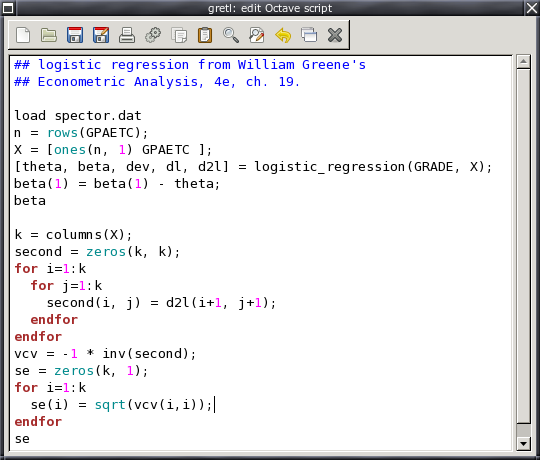
\includegraphics[scale=0.7]{figures/Octedit}
  \caption{\app{Octave} editing window}
  \label{fig:Octedit}
\end{figure}

\begin{figure}[htbp]
  \centering
  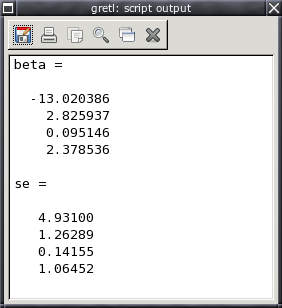
\includegraphics[scale=0.7]{figures/Octout}
  \caption{Output from \app{Octave}}
  \label{fig:Octout}
\end{figure}

In addition you can embed \app{Octave} code within a gretl
script using a \texttt{foreign} block, as described in connection with
\app{R}.  A trivial example, which simply loads and prints the
gretl data matrix within \app{Octave}, is shown below. (Note
that in \app{Octave}, appending ``\texttt{;}'' to a line suppresses
verbose output; leaving off the semicolon results in printing of the
object that is produced, if any.)
%
\begin{code}
open data4-1
matrix m = { dataset }
mwrite(m, "gretl.mat", 1)

foreign language=Octave
   gmat = gretl_loadmat("gretl.mat")
end foreign
\end{code}

We use the \texttt{mwrite} function to write a matrix into the user's
``dotdir'' (see section~\ref{sec:named-strings}), then in \app{Octave}
we use the function \verb|gretl_loadmat| to retrieve the matrix. The
``magic'' behind \verb|gretl_loadmat| works in essentially the same
way as for \app{Ox} (chapter~\ref{chap:gretlOx}).

\section{Illustration: spectral methods}
\label{sec:octave-coher}

We now present a more ambitious example which exploits \app{Octave}'s
handling of the frequency domain (and also its ability to use code
written for \app{MATLAB}), namely estimation of the spectral coherence
of two time series.  For this illustration we require two extra Octave
packages from \url{octave.sf.net}, namely those supporting spectral
functions (\texttt{specfun}) and signal processing (\texttt{signal}).
After downloading the packages you can install them from within
\app{Octave} as follows (using version numbers as of March 2010):
\begin{code}
pkg install specfun-1.0.8.tar.gz 
pkg install signal-1.0.10.tar.gz 
\end{code}

In addition we need some specialized \app{MATLAB} files made available
by Mario Forni of the University of Modena, at
\url{http://morgana.unimore.it/forni_mario/matlab.htm}. The files
needed are \texttt{coheren2.m}, \texttt{coheren.m}, \texttt{coher.m},
\texttt{cospec.m}, \texttt{crosscov.m}, \texttt{crosspec.m},
\texttt{crosspe.m} and \texttt{spec.m}. These are in a form appropriate
for MS Windows. On Linux you could run the following shell script
to get the files and remove the Windows end-of-file character (which
prevents the files from running under \app{Octave}):
\begin{code}
SITE=http://morgana.unimore.it/forni_mario/MYPROG
# download files and delete trailing Ctrl-Z
for f in \
  coheren2.m \
  coheren.m \
  coher.m \
  cospec.m \
  crosscov.m \
  crosspec.m \
  crosspe.m \
  spec.m ; do
    wget $SITE/$f && \
    cat $f | tr -d \\032 > tmp.m && mv tmp.m $f
done
\end{code}

The Forni files should be placed in some appropriate directory, and
you should tell \app{Octave} where to find them by adding that
directory to \app{Octave}'s \texttt{loadpath}. On Linux this can be
done via an entry in one's \verb|~/.octaverc| file. For example
\begin{code}
addpath("~/stats/octave/forni");
\end{code}
Alternatively, an \texttt{addpath} directive can be written into the
\app{Octave} script that calls on these files.

With everything set up on the \app{Octave} side we now write a gretl
script (see Example~\ref{Octave-coher}) which opens a time-series
dataset, constructs and writes a matrix containing two series, and
defines a \texttt{foreign} block containing the \app{Octave}
statements needed to produce the spectral coherence matrix. The matrix
is exported via the \verb|gretl_export| function, which is
automatically defined for you; this function takes two arguments, a
matrix and a file name.  The file is written into the user's
``dotdir'', from where it can be picked up using
\texttt{mread}. Finally, we produce a graph from the matrix in gretl.
In the script this is sent to the screen; Figure~\ref{fig:coherence}
shows the same graph in PDF format.

\begin{script}[htbp]
  \caption{Estimation of spectral coherence via \app{Octave}}
\begin{scode}
open data9-7
matrix xy = { PRIME, UNEMP }
mwrite(xy, "xy.mat", 1)

foreign language=Octave
 # uncomment and modify the following if necessary
 # addpath("~/stats/octave/forni");
 xy = gretl_loadmat("xy.mat");
 x = xy(:,1);
 y = xy(:,2);
 # note: the last parameter is the Bartlett window size
 h = coher(x, y, 8);
 gretl_export(h, "h.mat");
end foreign

h = mread("h.mat", 1)
colnames(h, "coherence")
gnuplot 1 --time-series --with-lines --matrix=h --output=display
\end{scode}
\label{Octave-coher}
\end{script}

\begin{figure}[htbp]
  \centering
  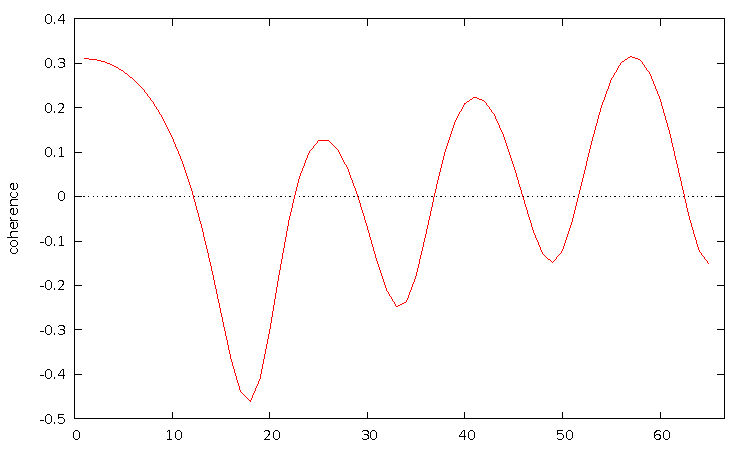
\includegraphics{figures/coherence}
  \caption{Spectral coherence estimated via \app{Octave}}
  \label{fig:coherence}
\end{figure}

%%% Local Variables: 
%%% mode: latex
%%% TeX-master: "gretl-guide"
%%% End: 


\chapter{Gretl and Stata}
\label{chap:gretlStata}

\app{Stata} (\url{www.stata.com}) is closed-source, proprietary (and
expensive) software and as such is not a natural companion to
\app{gretl}. Nonetheless, given \app{Stata}'s popularity it is
desirable to have a convenient way of comparing results across the two
programs, and to that end we provide limited support for \app{Stata}
code under the \texttt{foreign} command.

The following example illustrates what's available. You can send the
current \app{gretl} dataset to \app{Stata} using the
\option{send-data} flag. And having defined a matrix within
\app{Stata} you can export it for use with \app{gretl} via the
\verb|gretl_export| command: this takes two arguments, the name of the
matrix to export and the filename to use; the file is written to the
user's ``dotdir'', from where it can be retrieved using the
\texttt{mread()} function.\footnote{We do not currently offer the
  complementary functionality of \verb|gretl_loadmat|, which enables
  reading of matrices written by \app{gretl}'s \texttt{mwrite()}
  function in \app{Ox} and \app{Octave}. This is not at all easy to
  implement in \app{Stata} code.} To suppress printed output
from \app{Stata} you can add the \option{quiet} flag to the
\texttt{foreign} block.


\begin{script}[htbp]
  \caption{Comparison of clustered standard errors with \app{Stata}}
\begin{scode}
function matrix stata_reorder (matrix se)
  # stata puts the intercept last, but gretl puts it first
  scalar n = rows(se)
  return se[n] | se[1:n-1]
end function

open data4-1
ols 1 0 2 3 --cluster=bedrms
matrix se = $stderr

foreign language=stata --send-data
  regress price sqft bedrms, vce(cluster bedrms)
  matrix vcv = e(V)
  gretl_export vcv "vcv.mat"
end foreign

matrix stata_vcv = mread("@dotdir/vcv.mat")
stata_se = stata_reorder(sqrt(diag(stata_vcv)))
matrix check = se - stata_se
print check
\end{scode}
\label{Stata-test}
\end{script}

Note that there is no support for editing \app{Stata} scripts via the
\app{gretl} GUI. Also note that \app{Stata} coerces all variable
names to lower-case on data input, so even if series names in
\app{gretl} are upper-case, or of mixed case, it's necessary to use
all lower-case in \app{Stata}. 

%%% Local Variables: 
%%% mode: latex
%%% TeX-master: "gretl-guide"
%%% End: 


\chapter{Gretl and Python}
\label{chap:gretlPython}

\section{Introduction}
\label{Python-intro}

According to \url{www.python.org}, \app{Python} is ``an easy to learn,
powerful programming language. It has efficient high-level data
structures and a simple but effective approach to object-oriented
programming. Python's elegant syntax and dynamic typing, together with
its interpreted nature, make it an ideal language for scripting and
rapid application development in many areas on most platforms.''

Indeed, \app{Python} is widely used in a great variety of
contexts. Numerous add-on modules are available; the ones likely to be
of greatest interest to econometricians include \app{NumPy} (``the
fundamental package for scientific computing with Python'' --- see
\url{www.numpy.org}); \app{SciPy} (which builds on \app{NumPy} --- see
\url{www.scipy.org}); and \app{Statsmodels}
(\url{http://statsmodels.sourceforge.net/}).

\section{Python support in gretl}
\label{sec:Python-support}

The support offered for \app{Python} in \app{gretl} is similar to that
offered for \app{Octave} (chapter~\ref{chap:gretlOctave}). You can
open and edit \app{Python} scripts in the \app{gretl} GUI.  Clicking
the ``execute'' icon in the editor window will send your code to
\app{Python} for execution. In addition you can embed \app{Python}
code within a \app{gretl} script using a \texttt{foreign} block, as
described in connection with \app{R}.

When you launch \app{Python} from within \app{gretl} one variable and
two convenience functions are pre-defined, as follows.
\begin{code}
gretl_dotdir
gretl_loadmat(filename, autodot=1)
gretl_export(M, filename, autodot=1)
\end{code}
The variable \verb|gretl_dotdir| holds the path to the user's ``dot
directory.''  The first function loads a matrix of the given
\texttt{filename} as written by \app{gretl}'s \texttt{mwrite}
function, and the second writes matrix \texttt{M}, under the given
\texttt{filename}, in the format wanted by \app{gretl}.

By default the traffic in matrices goes via the dot directory on the
\app{Python} side; that is, the name of this directory is prepended to
\texttt{filename} for both reading and writing. (This is complementary
to use of the \textsl{export} and \textsl{import} parameters with
\app{gretl}'s \texttt{mwrite} and \texttt{mread} functions,
respectively.) However, if you wish to take control over the reading
and writing locations you can supply a zero value for
\texttt{autodot} when calling \verb|gretl_loadmat| and
\verb|gretl_export|: in that case the \texttt{filename} argument is
used as is.

Note that \verb|gretl_loadmat| and \verb|gretl_export| depend on
\app{NumPy}; they make use of the functions \texttt{loadtxt} and
\texttt{savetxt} respectively. Nonetheless, the presence of
\app{NumPy} is not an absolute requirement if you don't need
to use these two functions.

\section{Illustration: linear regression with multicollinearity}
\label{sec:Python-longley}

Example~\ref{Python-longley} compares the numerical accuracy of
\app{gretl}'s \texttt{ols} command with that of \app{NumPy}'s
\texttt{linalg.lstsq}, using the notorious Longley test data which
exhibit extreme multicollinearity.  Unlike some econometrics packages,
\app{NumPy} does a good job on these data. The script computes and
prints the log-relative error in estimation of the regression
coefficients, using the NIST-certified values as a
benchmark;\footnote{See
  \url{http://www.itl.nist.gov/div898/strd/lls/data/Longley.shtml}.}
the error values correspond to the number of correct digits (with a
maximum of 15). The results will differ somewhat by computer
architecture; the output shown was obtained on a 32-bit Linux Intel i5
system.

\begin{script}[htbp]
  \caption{Comparing regression results with \app{Python}}
\begin{scode}
set echo off
set messages off

function matrix logrel_error (matrix est, matrix true)
  return -log10(abs(est - true) ./ abs(true))
end function

open longley.gdt -q
list LX = prdefl .. year
# gretl's regular OLS
ols employ 0 LX -q
matrix b = $coeff

mwrite({employ}, "y.mat", 1)
mwrite({const} ~ {LX}, "X.mat", 1)

foreign language=python
   import numpy as np
   y = gretl_loadmat('y.mat', 1)
   X = gretl_loadmat('X.mat', 1)
   # NumPy's OLS   
   b = np.linalg.lstsq(X, y)[0]
   gretl_export(np.transpose(np.matrix(b)), 'py_b.mat', 1)
end foreign

# NIST's certified coefficient values
matrix nist_b = {-3482258.63459582, 15.0618722713733,
    -0.358191792925910E-01, -2.02022980381683,
    -1.03322686717359, -0.511041056535807E-01,
     1829.15146461355}'

matrix py_b = mread("py_b.mat", 1)
matrix errs = logrel_error(b, nist_b) ~ logrel_error(py_b, nist_b)
colnames(errs, "gretl python")
printf "Log-relative errors, Longley coefficients:\n\n%12.5g\n", errs
printf "Column means\n%12.5g\n", meanc(errs)
\end{scode}
Output:
\begin{code}
Log-relative errors, Longley coefficients:

       gretl      python
      12.844       12.85
      11.528      11.414
      12.393      12.401
      13.135      13.121
      13.738      13.318
      12.587      12.363
      12.848      12.852

Column means
      12.725      12.617
\end{code}
\label{Python-longley}
\end{script}

%%% Local Variables: 
%%% mode: latex
%%% TeX-master: "gretl-guide"
%%% End: 


\chapter{Risoluzione dei problemi}
\label{trouble}



\section{Segnalazione dei bug}
\label{trouble-bugs}


Le segnalazioni dei bug sono benvenute. � difficile trovare errori di
calcolo in \app{gretl} (ma questa affermazione non costituisce alcuna
sorta di garanzia), ma � possibile imbattersi in bug o stranezze nel
comportamento dell'interfaccia grafica. Si tenga presente che
l'utilit� delle segnalazioni aumenta quanto pi� si � precisi nella
descrizione: cosa \emph{esattamente} non funziona, in che condizioni,
con quale sistema operativo? Se si ricevono messaggi di errore, cosa
dicono esattamente?

\section{Programmi ausiliari}
\label{trouble-programs}

Come detto in precedenza, \app{gretl} richiama alcuni altri programmi
per eseguire alcune operazioni (gnuplot per i grafici, {\LaTeX} per la
stampa ad alta qualit� dei risultati delle regressioni, GNU R).  Se
succede qualche problema durante questi collegamenti esterni, non �
sempre facile per \app{gretl} fornire un messaggio di errore abbastanza informativo.
Se il problema si verifica durante l'uso di \app{gretl} con
l'interfaccia grafica, pu� essere utile avviare \app{gretl} da un terminale
invece che da un men� o da un'icona del desktop. Se si usa il sistema
X window, � sufficiente avviare gretl dal prompt dei comandi di un 
\app{xterm}, mentre se si usa MS Windows occorre digitare \cmd{gretlw32.exe} da
una finestra di terminale, o ``Prompt di MS-DOS'', usando le opzioni \verb|-g|
o \verb|--debug|. Il terminale conterr� quindi messaggi di errore aggiuntivi.

Si tenga anche presente che nella maggior parte dei casi \app{gretl}
assume che i programmi in questione siano disponibili nel ``percorso
di esecuzione'' (path) dell'utente, ossia che possano essere invocati
semplicemente con il nome del programma, senza indicare il percorso
completo\footnote{L'eccezione a questa regola � costituita
  dall'invocazione di gnuplot in MS Windows, dove occorre indicare il
  percorso completo del programma.}.  Quindi se un certo programma non
si avvia, conviene provare ad eseguirlo da un prompt dei comandi, come
descritto di seguito.
      
\begin{center}
  \begin{tabular}{llll}
    & \textit{Grafica} & \textit{Stampa} & \textit{GNU R}\\
    Sistema X window & gnuplot & latex, xdvi & R\\
    MS Windows & wgnuplot.exe & pdflatex & RGui.exe\\
  \end{tabular}
\end{center}

Se il programma non si avvia dal prompt, non � un problema di
\app{gretl}: probabilmente la directory principale del programma non �
contenuta nel path dell'utente, oppure il programma non � stato
installato correttamente.  Per i dettagli su come modificare il path
dell'utente, si veda la documentazione o l'aiuto online per il proprio
sistema operativo.
    
%%% Local Variables: 
%%% mode: latex
%%% TeX-master: "gretl-guide-it"
%%% End: 


\chapter{O interface de linha de comandos (CLI)}
\label{cli}

A aplica��o \app{gretl} inclui o programa de linha de comandos \app{gretlcli}.
Em Linux pode ser iniciado a partir de uma janela de terminal (xterm,
rxvt, ou semelhante), ou de uma consola de texto.  No MS Windows pode ser 
executado numa janela de linha de comandos (algumas vezes incorrectamente
chamada de ``janela MS DOS'').
\app{gretlcli} tem o seu pr�prio ficheiro de ajuda, que pode ser acedido
escrevendo o comando ``help'' no interface CLI. Pode ser executado em modo de
sequ�ncia de comandos, enviando os resultados directamente para um ficheiro
(ver tamb�m o \GCR).
    
Se \app{gretlcli} tiver sido ligado no momento da compila��o � biblioteca de
programas \app{readline} (o que acontece sempre no caso da vers�o MS Windows;
ver tamb�m Ap�ndice~\ref{app-build}), � poss�vel repetir e editar as linhas
de comandos, e tamb�m completar comandos automaticamente.  Voc� pode usar as
teclas seta-Acima e seta-Abaixo para percorrer os comandos anteriormente
executados.  Numa dada linha de comando, voc� pode usar as setas para mover o
cursor, em conjunto com as combina��es de teclas do editor Emacs.\footnote{Na realidade, as combina��es de  teclas referidas abaixo s�o apenas as definidas por omiss�o; elas poder�o ser personalizadas por si.
  Ver o \href{http://cnswww.cns.cwru.edu/~chet/readline/readline.html}{manual
    do readline}.} As mais comuns s�o:
%    
\begin{center}
  \begin{tabular}{cl}
    \textit{Combina��o} & \multicolumn{1}{c}{\textit{Efeito}}\\
    \verb+Ctrl-a+ & ir para o in�cio da linha\\
    \verb+Ctrl-e+ & ir para o fim da linha\\
    \verb+Ctrl-d+ & apagar o caracter � direita\\
  \end{tabular}
\end{center}
%
onde ``\verb+Ctrl-a+'' significa premir a tecla ``\verb+a+'' ao mesmo tempo
que a tecla ``\verb+Ctrl+'' � premida.  Assim, se voc� quiser alterar algo no
in�cio de um comando, voc� \emph{n�o} precisa de apagar caracter a caracter
na linha toda.  Basta saltar para o in�cio e acrescentar ou apagar caracteres.
Se voc� escrever as primeiras letras de um comando e pressionar a tecla Tab, o
sistema \app{readline} vai tentar completar o comando por voc�.  Se houver uma
�nica possibilidade, o comando � automaticamente completado.  Se houver mais
que uma, pressionando Tab uma segunda vez faz aparecer uma lista.

Provavelmente o modo mais produtivo para an�lises intensivas com o
\app{gretlcli} � em modo de sequ�ncia de comandos (n�o-interactivo), no qual o
programa l� e processa um ficheiro de sequ�ncia de comandos, e envia a sa�da
para um ficheiro.  Por exemplo
\begin{code}
gretlcli -b ficheirodecomandos > ficheiroderesultados
\end{code}

O \textsl{ficheirodecomandos} � tratado como um argumento de programa; apenas o ficheiro de resultados requer redirecionamento (\verb|>|).  N�o esquecer a op��o \texttt{-b}
(\textit{batch}=lote), de outro modo o programa ficar� a aguardar comandos do
utilizador ap�s a execu��o da sequ�ncia de comandos (e se a sa�da estiver redirecionada, o programa aparentar� estar "pendurado").

    
%%% Local Variables: 
%%% mode: latex
%%% TeX-master: "gretl-guide-pt"
%%% End: 



\part{Appendices}

\begin{appendices}
\chapter{Dettagli sui file di dati}
\label{app-datafile}

\section{Formato interno di gretl}
\label{native}

Il formato dati usato internamente da \app{Gretl} per i dataset �
basato su XML (extensible mark-up language).  I file di dati sono conformi al
semplice DTD (document type definition) contenuto nel file
\verb+gretldata.dtd+, fornito con la distribuzione di \app{Gretl} e
installato nella directory dei dati di sistema (ad es.
\verb+/usr/share/gretl/data+ su Linux). I file di dati possono essere
non compressi o compressi con gzip; oltre ai valori dei dati,
essi contengono altre informazioni aggiuntive, come i nomi e le descrizioni
delle variabili, la frequenza dei dati e cos� via.

La maggior parte degli utenti probabilmente non avr� bisogno di
leggere o scrivere questi file, se non usando \app{Gretl} stesso, ma
se si vuole manipolarli usando altri strumenti, pu� essere utile
esaminare il DTD e qualcuno dei file di esempio forniti: il file
\verb+data4-1.gdt+ d� un semplice esempio, il file \verb+data4-10.gdt+
invece contiene anche delle etichette per le osservazioni.

\section{Formato tradizionale di ESL}
\label{traddata}

Per compatibilit� all'indietro, \app{Gretl} pu� elaborare anche file
di dati nel formato ``tradizionale'' usato dal programma \app{ESL}
di Ramanathan.  In questo formato (che era quello predefinito nelle
versioni di \app{Gretl} precedenti alla 0.98) un dataset �
rappresentato da due file: uno contiene i dati veri e propri, l'altro
contiene la descrizione dei dati e le modalit� per la loro lettura.
In particolare:

\begin{enumerate}
\item \emph{Dati veri e propri}: una matrice rettangolare di numeri
  separati da spazi vuoti. Ogni colonna rappresenta una variabile,
  ogni riga un'osservazione per ognuna delle variabili (come in un
  foglio elettronico). Le colonne dei dati possono essere separate da
  spazi o caratteri tab. Il nome del file deve avere l'estensione
  \verb+.gdt+ e il file di solito � di tipo ASCII (testo semplice), ma
  pu� essere anche compresso con gzip, per occupare meno spazio su
  disco. � possibile inserire commenti in un file di dati: se una riga
  comincia con un carattere cancelletto (\verb+#+), l'intera riga
  viene ignorata (questo comportamento � coerente con i file di dati
  di gnuplot e di octave).
\item \emph{Descrizione}: il file di dati deve essere accompagnato da
  un file di descrizioni, che ha lo stesso nome di base del file di
  dati, ma l'estensione \verb+.hdr+.  Questo file contiene,
  nell'ordine:

  \begin{itemize}
  \item (Opzionale) \emph{commenti} sui dati, introdotti dalla stringa
    di apertura \verb+(*+ e conclusi dalla stringa \verb+*)+; ognuna
    di queste stringhe deve essere presente da sola su una riga.
  \item (Richiesta) lista dei \emph{nomi delle variabili} presenti nel
    file, separati da spazio bianco. I nomi sono limitati a 8
    caratteri, devono iniziare con una lettera e possono contenere
    solo caratteri alfanumerici e il carattere trattino basso,
    \verb+_+. La lista pu� continuare su pi� righe e deve essere
    chiusa da un punto e virgola \verb+;+.
  \item (Richiesta) riga \emph{osservazioni}, nel formato 
    \verb+1 1 85+. Il primo elemento indica la frequenza dei dati (1 per dati
    non datati o annuali, 4 per trimestrali, 12 per mensili).  Gli
    altri due elementi indicano le osservazioni iniziale e finale: di
    solito questi saranno pari a 1 e al numero delle osservazioni, per
    i dati non datati. Per le serie storiche, � possibile usare date
    nella forma \cmd{1959.1} (trimestrale, una cifra dopo il punto) o
    \cmd{1967.03} (mensile, due cifre dopo il punto). Si veda il
    capitolo~\ref{chap-panel} per l'uso speciale di questa riga nel
    caso dei dati panel.
  \item La parola chiave \verb+BYOBS+.
  \end{itemize}
\end{enumerate}

Ecco un esempio di un file di descrizione dei dati ben scritto.
        
\begin{code}
(* 
  DATA9-6: 
  Dati su log(moneta), log(reddito) e tasso di interesse USA. 
  Fonte: Stock and Watson (1993) Econometrica 
  (dati grezzi) Il periodo � 1900-1989 (dati annuali). 
  Dati composti da Graham Elliott. 
*) 
lmoneta lreddito tassint ; 
1 1900 1989 BYOBS
\end{code}
          
Il corrispondente file di dati contiene tre colonne di dati, ognuna
con 90 osservazioni.  Ci sono altre tre caratteristiche del formato
dati ``tradizionale'' degne di nota.
    
\begin{enumerate}
\item Se la parola chiave \verb+BYOBS+ � sostituita da \verb+BYVAR+ ed
  � seguita dalla parola chiave \verb+BINARY+, significa che il
  corrispondente file di dati � in formato binario. Questo tipo di
  file di dati pu� essere scritto da \app{gretlcli} usando il comando
  \cmd{store} con l'opzione \cmd{-s} (precisione singola) o l'opzione
  \cmd{-o} (precisione doppia).
\item Se \verb+BYOBS+ � seguita dalla parola chiave \verb+MARKERS+,
  \app{Gretl} si aspetta un file di dati in cui la \emph{prima
    colonna} contiene stringhe (lunghe al massimo 8 caratteri) usate
  per identificare le osservazioni. Queste possono essere utili nel
  caso dei dati di tipo cross-section in cui le unit� di osservazione
  sono identificabili: regioni, stati, citt� ecc. Un altro caso �
  quello delle serie storiche irregolari, come ad esempio i dati
  giornalieri delle quotazioni azionarie, in cui mancano i giorni in
  cui non avvengono contrattazioni: in questo caso, le osservazioni
  possono essere marcate con una stringa che rappresenta la data, come
  ad esempio \cmd{10/01/98} (si ricordi il limite di 8 caratteri). Si
  noti che le opzioni \cmd{BINARY} e \cmd{MARKERS} sono mutualmente
  esclusive, e si noti anche che i ``marcatori'' non sono considerati
  come una variabile: questa colonna non compare nell'elenco delle
  variabili nel file di descrizione dei dati.
\item Se esiste un file con lo stesso nome di base del file di dati e
  di quello delle descrizioni, ma con l'estensione \verb+.lbl+, esso
  viene letto e usato per riempire le etichette descrittive per le
  serie di dati. Il formato del file di etichette � semplice: ogni
  riga contiene il nome di una variabile (indicata nel file di
  descrizione) seguito da uno o pi� spazi, seguito dall'etichetta
  descrittiva. Ecco un esempio:
  \verb+prezzo Indice dei prezzi auto nuove, anno base 1982+ 

\end{enumerate}

Se si vuole salvare i dati nel formato tradizionale, occorre usare
l'opzione \cmd{-t} con il comando \cmd{store}, nella versione a riga
di comando del programma o nella finestra del terminale della versione
grafica del programma.

\section{Dettagli sui database binari}
\label{dbdetails}

Un database di \app{Gretl} consiste di due parti: un file indice ASCII
(con l'estensione \verb+.idx+) che contiene informazioni sulle serie,
e un file binario (con estensione \verb+.bin+) che contiene i dati
veri e propri. Ecco due esempi di voci contenute in un file
\verb+idx+:

\begin{code}
G0M910  Indice composto da 11 indicatori principali (1987=100) 
M 1948.01 - 1995.11  n = 575
currbal Bilancia dei pagamenti: parte corrente; corretta per la stagionalit�
Q 1960.1 - 1999.4 n = 160
\end{code}

Il primo campo � il nome della serie, il secondo � una descrizione
della serie (al massimo di 128 caratteri). Sulla seconda riga, il
primo campo � un codice di frequenza: \verb+M+ per dati mensili, \verb+Q+
per dati trimestrali, \verb+A+ per dati annuali, \verb+B+ per dati
giornalieri-lavorativi (giornalieri con cinque giorni a settimana) e
\verb+D+ per dati giornalieri (sette giorni a settimana). Al momento non
vengono accettati altri codici di frequenza. Quindi segue la data
iniziale (con due cifre che seguono il punto nei dati mensili, una per
i dati trimestrali, nessuna per quelli annuali), uno spazio, un
trattino, un altro spazio, la data finale, la stringa ``\verb+n = +''
e il numero delle osservazioni. Nel caso di dati giornalieri, le date
iniziale e finale devono essere indicate nella forma
\verb+YYYY/MM/DD+. Questo formato deve essere rispettato alla
lettera.

Opzionalmente, la prima riga del file indice pu� contenere un breve
commento (al massimo 64 caratteri) a proposito della fonte e del tipo
dei dati, che segue un carattere cancelletto. Ad esempio:
      
\begin{code}
# Banca Centrale Europea (tassi di interesse)
\end{code}

Il corrispondente database binario contiene i valori dei dati,
rappresentati come ``float'', ossia come numeri in virgola mobile a
precisione singola, che tipicamente occupano quattro byte ciascuno. I
numeri sono immagazzinati ``per variabile'', cos� che i primi \emph{n}
numeri sono le osservazioni della variabile 1, i successivi \emph{m}
sono le osservazioni per la variabile 2 e cos� via.

\chapter{Compilare \app{gretl}}
\label{app-build}

\section{Requisiti}
\label{sec:build-req}

\app{Gretl} � scritto nel linguaggio di programmazione C, aderendo
nel modo pi� stretto possibile allo standard C ISO/ANSI (C90), anche
se l'interfaccia grafica e alcune altre componenti devono fare uso
necessariamente di estensioni specifiche per certe piattaforme.
  
Il programma � sviluppato in ambiente Linux.  La libreria condivisa e
il client a riga di comando dovrebbero essere compilabili su qualsiasi
piattaforma che supporti l'ISO/ANSI C e abbia installate le
librerie elencate nella Tabella~\ref{tab:depend}. Se il sistema
dispone anche della libreria GNU readline, essa sar� usata per
\app{gretcli}, fornendo una riga di comando molto pi� comoda da
utilizzare.  Si veda la
\href{http://cnswww.cns.cwru.edu/~chet/readline/rltop.html}{home page
  di readline}.  

\begin{table}[htbp]
  \centering
  \begin{tabular}{lll}
\textit{Libreria} & \textit{Funzione} & \textit{Sito web} \\ [4pt]
zlib & compressione dei dati &  
   \href{http://www.info-zip.org/pub/infozip/zlib/}{info-zip.org} \\
libxml2 & manipolazione XML &
   \href{http://xmlsoft.org/}{xmlsoft.org} \\
LAPACK & algebra lineare & 
   \href{http://www.netlib.org/lapack/}{netlib.org} \\
FFTW3 & Trasformata veloce di Fourier & 
   \href{http://www.fftw.org/}{fftw.org} \\
glib-2.0 & Varie utilit� & 
  \href{http://www.gtk.org/}{gtk.org}
  \end{tabular}
  \caption{Librerie richieste per compilare gretl}
  \label{tab:depend}
\end{table}

Il client grafico dovrebbe essere compilabile e utilizzabile su ogni
sistema che, oltre ai requisiti visti sopra, offra la libreria GTK
nella versione 2.4.0 o superiore (si veda
\href{http://www.gtk.org/}{gtk.org})\footnote{Fino alla versione 1.5.1,
\app{gretl} poteva essere compilato anche usando GTK 1.2, ma il supporto per
questa libreria � stato abbandonato a partire dalla versione 1.6.0 di \app{gretl}.}.

\app{Gretl} usa gnuplot per produrre grafici. � possibile trovare
gnuplot a \href{http://www.gnuplot.info/}{gnuplot.info}. Al momento
della scrittura di questo manuale, la versione ufficiale pi� recente
di gnuplot � la 4.2 (di marzo 2007).  La versione MS Windows di
\app{Gretl} comprende la versione 4.2 di gnuplot per Windows; sul sito
web di Gretl � possibile trovare un pacchetto rpm di gnuplot 3.8j0 per
sistemi Linux x86.
  
Alcune funzionalit� di \app{Gretl} fanno uso di parti della libreria
\app{gtkextra} di Adrian Feguin.  Le parti rilevanti di questo pacchetto sono
incluse (in forma leggermente modificata) con la distribuzione sorgente di
\app{gretl}.
  
Una versione binaria del programma � disponibile per la piattaforma
Microsoft Windows (Windows 98 o superiore).
Questa versione � cross-compilata su Linux usando mingw (il
compilatore GNU C, \app{gcc}, portato per l'uso con win32) e collegata
alla libreria C di Microsoft C, \verb+msvcrt.dll+. Utilizza il port di
GTK 2.0 su win32 di Tor Lillqvist. L'installatore per Windows (libero,
open-source) � a cura di Jordan Russell
(\href{http://www.jrsoftware.org/}{jrsoftware.org}).  

Speriamo che gli utenti con conoscenze di programmazione possano
considerare \app{Gretl} abbastanza interessante e degno di essere
migliorato ed esteso. La documentazione dell'API libgretl non � ancora
completa, ma � possibile trovare alcuni dettagli seguendo il link
``Libgretl API docs'' sul sito web di \app{Gretl}. Chiunque sia interessato
allo sviluppo di \app{gretl} � invitato a iscriversi alla mailing list
\href{http://gretl.sourceforge.net/lists.html}{gretl-devel}.

\section{Istruzioni per la compilazione}
\label{sec:build-inst}

Questa sezione contiene istruzioni che permettono di compilare \app{gretl}
a un utente con una conoscenza di base di un sistema di tipo Unix.
La procedura � stata testata su una nuova installazione della distribuzione
Debian Etch e dovrebbe funzionare anche su altre distribuzioni Linux
(specialmente quelle derivate da Debian, come Ubuntu e simili). Su altri sistemi
simili a Unix, come MacOSX e BSD, potrebbero esserci differenze maggiori nella
procedura.

In questo esempio guidato, compileremo \app{gretl} insieme alla sua
documentazione completa. Questa scelta implica alcuni requisiti in pi�, ma in
cambio permette di modificare anche i file della documentazione, come l'aiuto in
linea o i manuali.

\subsection{Installare i programmi di base}

Assumiamo che le utilit� GNU di base siano gi� installate sul sistema, insieme
a questi altri programmi:
\begin{itemize}
  \item Un sistema \TeX/\LaTeX (\texttt{tetex} o \texttt{texlive} vanno
    benissimo)
  \item Gnuplot
  \item ImageMagick
\end{itemize}
Assumiamo anche che l'utente abbia i privilegi di amministratore e sappia come
installare i pacchetti. Gli esempi seguenti mostrano  l'uso del comando shell
\texttt{apt-get}, ma possono essere replicati anche con comandi come
\texttt{aptitude}, \texttt{dselect}, con il programma a interfaccia grafica
\texttt{synaptic}. Gli utenti di distribuzioni Linux che usano pacchetti rpm
(es.\ Red Hat/Fedora, Mandriva, SuSE) possono consultare la pagina
\href{http://gretl.sourceforge.net/depend_it.html}{dipendenze} sul sito di
\app{gretl}.

Il primo passo consiste nell'installare il compilatore C e le utilit� correlate.
Su un sistema Debian, occorre installare i seguenti pacchetti:
\begin{code}
apt-get install gcc autoconf automake1.9 libtool flex bison gcc-doc \
libc6-dev libc-dev libgfortran1 libgfortran1-dev gettext pkgconfig
\end{code}

Quindi occorre installare i pacchetti ``di sviluppo'' (\texttt{dev})
per le librerie usate da \app{gretl}:

\begin{center}
  \begin{tabular}{ll}
    \textit{Libreria} & \textit{Comando} \\ [4pt]
    GLIB & \texttt{apt-get install libglib2.0-dev} \\
    GTK 2.0 & \texttt{apt-get install libgtk2.0-dev} \\
    PNG & \texttt{apt-get install libpng12-dev} \\
    XSLT & \texttt{apt-get install libxslt1-dev} \\
    LAPACK & \texttt{apt-get install lapack3-dev} \\
    FFTW & \texttt{apt-get install fftw3-dev} \\
    READLINE & \texttt{apt-get install libreadline5-dev} \\
    GMP & \texttt{apt-get install libgmp3-dev}
  \end{tabular}
\end{center}

GMP � opzionale, ma raccomandata.  I pacchetti \texttt{dev} di queste librerie
sono necessari per \emph{compilare} \app{gretl}, mentre per \emph{eseguire} il
programma occorrono anche i pacchetti normali (non-\texttt{dev}) delle librerie;
la maggior parte di questi pacchetti fa gi� parte delle installazioni standard.
Per abilitare funzionalit� aggiuntive, come il supporto audio, occorre
installare altre librerie.

\subsection{Procurarsi il sorgente: pacchetto o CVS}

A questo punto � possibile iniziare a compilare il sorgente. � possibile
procurarselo in due modi: scaricando l'ultimo pacchetto sorgente rilasciato, o
scaricando la versione di \app{gretl} contenuta attualmente nell'archivio CVS
(Concurrent Versions System). La versione CVS � di solito pi� recente, pu�
contenere correzioni di bug presenti nell'ultimo pacchetto rilasciato, ma pu�
anche contenere nuovi bug (o addirittura non essere compilabile) e codice
``sperimentale''. Se si vuole partecipare allo sviluppo e al test del programma,
� raccomandabile usare la versione CVS di \app{gretl}.

Per lavorare col pacchetto sorgente:

\begin{enumerate}
  \item Scaricare il pacchetto dei sorgenti di \app{Gretl}
    da \href{http://gretl.sourceforge.net/}{gretl.sourceforge.net}.
  \item Decomprimere il pacchetto. Se si dispone delle utilit� GNU,
    usare il comando \cmd{tar xvfz gretl-N.tar.gz} (sostituire \cmd{N}
    con il numero di versione specifico del file scaricato).
  \item Spostarsi nella directory del codice sorgente di gretl appena
    creata (ad es. \verb+gretl-1.6.6+).
  \item Procedere alla sezione seguente ``Configurare il sorgente''.
\end{enumerate}
          
Per lavorare con CVS occorre per prima cosa installare il programma client \app{cvs},
se non si trova gi� sul proprio sistema. Pu� essere utile consultare il sito web
di CVS \href{http://www.nongnu.org/cvs/}{www.nongnu.org/cvs}, le istruzioni per
l'uso di CVS su SourceForge contenute nella
\href{http://sourceforge.net/docman/display_doc.php?docid=14035&group_id=1}{pagina
CVS di SourceForge}, e le istruzioni specifiche su \app{gretl} nella
\href{http://sourceforge.net/cvs/?group_id=36234}{pagina CVS di Gretl}.

Quando si scarica il codice da CVS \textit{per la prima volta}, occorre decidere
dove salvarlo. Ad esempio si pu� creare una directory chiamata \texttt{cvs}
nella propria home directory, aprire un terminale, fare \texttt{cd} in questa
directory ed eseguire i comandi seguenti:
%
\begin{code}
cvs -d:pserver:anonymous@gretl.cvs.sourceforge.net:/cvsroot/gretl login
cvs -z3 -d:pserver:anonymous@gretl.cvs.sourceforge.net:/cvsroot/gretl co -P gretl
\end{code}
%
Dopo il primo comando verr� richiesta una password: basta premere invio. Dopo il
secondo comando, \app{cvs} creer� una sotto-directory chiamatat \texttt{gretl}
che conterr� il codice sorgente.

Ogni volta che si vuole \textit{aggiornare la propria copia del sorgente}, basta
andare nella directory \texttt{gretl} ed eseguire
\begin{code}
cvs update -d -P
\end{code}

Da questo punto in poi, assumendo di essere nella directory \texttt{gretl}, �
possibile seguire le istruzioni valide anche per il sorgente contenuto nel
pacchetto.

\subsection{Configurare il sorgente}

Il successivo comando da eseguire � \texttt{./configure}; si tratta di uno
script sofisticato che cerca gli strumenti disponibili sul sistema e prepara
la compilazione. Il comando \texttt{configure} accetta molte opzioni: eseguendo
\begin{code}
./configure --help
\end{code}
si ottiene l'elenco di quelle disponibili. Un'opzione che pu� essere utile usare
� \cmd{--prefix}, che modifica il percorso principale in cui verr� installato il
programma; il valore predefinito � \verb+/usr/local+. Ad esempio usando
\begin{code}
./configure --prefix=/usr
\end{code}
i file verranno installati sotto il percorso \verb+/usr+. Un'altra opzione ha a
che fare col supporto per il desktop \app{gnome}, che \app{gretl} offre in
modalit� predefinita. Se non si � interessati alle funzionalit� specifiche di
\app{gnome} � possibile usare l'opzione
\verb+--without-gnome+ di \cmd{configure}.

Per compilare anche la documentazione, c'� un'altra opzione di
\texttt{configure}:
\begin{code}
./configure --enable-build-doc
\end{code}
Quando si esegue il comando, si vedranno i risultati di una serie di controlli,
e se tutto funziona correttamente, un riassunto finale simile a quello mostrato
nell'Esempio~\ref{configure-output}.

\begin{script}[htbp]
  \caption{Risultato di \texttt{./configure --enable-build-doc}}
  \label{configure-output}
\begin{scode}
Configuration:

  Installation path:                      /usr/local
  Use readline library:                   yes
  Use gnuplot for graphs:                 yes
  Use PNG for gnuplot graphs:             yes
  Use LaTeX for typesetting output:       yes
  Gnu Multiple Precision support:         yes
  MPFR support:                           no
  LAPACK support:                         yes
  FFTW3 support:                          yes
  Build with GTK version:                 2.0
  Script syntax highlighting:             yes
  Use installed gtksourceview:            yes
  Build with gnome support:               no
  Build gretl documentation:              yes
  Build message catalogs:                 yes
  Gnome installation prefix:              NA
  X-12-ARIMA support:                     yes
  TRAMO/SEATS support:                    yes
  Experimental audio support:             no

Now type 'make' to build gretl.
\end{scode}
\end{script}

\tip{Se si usa CVS, � una buona idea ri-eseguire lo script
  \texttt{configure} dopo ogni operazione di aggiornamento del sorgente.
  Non � sempre necessario, ma alcune volte lo �; in ogni caso non � dannoso.
  A questo proposito, pu� essere comodo creare un piccolo script di shell che
  esegue \texttt{configure} con le opzioni che si � soliti utilizzare.}

\subsection{Compilare e installare}

Siamo quindi pronti per iniziare la vera e propria compilazione: questa si
ottiene col comando \texttt{make}, che compila tutti i file sorgenti nell'ordine
corretto. Basta semplicemente eseguire
\begin{code}
make 
\end{code}

Questo passo della procedura richieder� qualche minuto e produrr� molti messaggi
sullo schermo. Alla fine, per installare la copia di \app{gretl} appena
prodotta, baster� eseguire:
\begin{code}
make install
\end{code}

Sulla maggior parte dei sistemi, il comando \texttt{make install} richiede di avere
i privilegi di amministratore di sistema. Quindi occorrer� fare login come
\texttt{root} prima di eseguirlo, oppure occorrer� usare il comando
\texttt{sudo}:
\begin{code}
sudo make install
\end{code}

\chapter{Accuratezza numerica}
\label{app-accuracy}

\app{Gretl} usa aritmetica a doppia precisione, ad eccezione del
plugin per precisione multipla invocabile con il comando del men�
``Modello, Altri modelli lineari, Minimi quadrati in alta precisione'' che rappresenta i
valori in virgola mobile usando un numero di bit indicato dalla
variabile di ambiente \verb+GRETL_MP_BITS+ (valore predefinito: 256).

Le equazioni normali dei minimi quadrati sono risolte in modo
predefinito usando la decomposizione di Cholesky, che � abbastanza
accurata per la maggior parte delle applicazioni. Nel caso le variabili
indipendenti esibiscano un'alto grado di collinearit�, \app{gretl} adotta
automaticamente la decomposizione QR; inoltre l'utente pu� scegliere di usare
sempre la decomposizione QR.

Il programma � stato testato abbastanza approfonditamente con i dataset di
riferimento forniti dal NIST (il National Institute of Standards and Technology
statunitense) e un rapporto completo dei risultati si trova sul sito web di
Gretl (seguendo il link ``Accuratezza numerica'').

Ad oggi, sono state pubblicate due recensioni che hanno preso in esame
l'accuratezza di \app{gretl}: Giovanni Baiocchi e Walter Distaso (2003), e Talha
Yalta e Yasemin Yalta (2007). Siamo grati a questi autori per il loro accurato
esame del programma. I loro commenti hanno suggerito vari miglioramenti, come
l'uso del codice \app{cephes} di Stephen Moshier per calcolare i p-value e altre
quantit� relative alle distribuzioni di probabilit� (si veda
\href{http://www.netlib.org/cephes/}{netlib.org}), modifiche alla formattazione
dei risultati delle regressioni per assicurare che il programma mostri un numero
coerente di cifre significative, soluzione di alcuni problemi di compilazione
della versione MS Windows di \app{gretl} (che in passato era leggermente meno
accurata della versione Linux).

La versione attuale di \app{Gretl} comprende un ``plugin'' che esegue
la suite NIST di test della regressione lineare. � possibile trovarlo
nel men� ``Strumenti'' della finestra principale. Quando viene eseguito
questo test, un'introduzione spiega qual � il risultato atteso: se si
esegue il test e si ottengono risultati diversi da quelli attesi, si
prega di inviare un bug report a \verb+cottrell@wfu.edu+.  

Tutte le statistiche di regressione sono mostrate
con 6 cifre significative nella versione attuale di \app{Gretl}
(tranne quando viene usato il plugin per precisione multipla, e allora
i risultati sono mostrati con 12 cifre). Se occorre esaminare un
valore pi� da vicino, basta per prima cosa salvarlo (si veda il
comando \cmd{genr}) e poi visualizzarlo usando il comando \cmd{printf}.


\chapter{Altro software libero utile}
\label{app-advanced}

Le possibilit� offerte da \app{gretl} sono molte e in continua espansione,
tuttavia pu� esserci l'esigenza di compiere operazioni non disponibili in
\app{gretl}, oppure di confrontare i risultati con quelli di altri programmi.
Se si � interessati a funzionalit� complementari disponibili nell'ambito del
software libero, o open source, raccomandiamo i programmi seguenti, di cui
riportiamo la descrizione fornita nei rispettivi siti web.

\begin{itemize}

\item \textbf{GNU R} \href{http://www.r-project.org/}{r-project.org}:
  ``R � un sistema per il calcolo statistico e i grafici. Consiste in
  un linguaggio e in un ambiente di lavoro che fornisce grafici, un
  debugger, l'accesso alle funzioni del sistema e la possibilit� di eseguire
  programmi contenuti all'interno di script\dots\ � compilabile ed eseguibile
  su un'ampia variet� di piattaforme UNIX, Windows e MacOS''.
  Commento: esistono molti pacchetti aggiuntivi per R, che coprono le principali
  aree dell'analisi statistica.

\item \textbf{GNU Octave}
  \href{http://www.octave.org/}{www.octave.org}:
  ``GNU Octave � un linguaggio ad alto livello, dedicato principalmente al
  calcolo numerico. Fornisce una comoda interfaccia a riga di comando per
  risolvere numericamente problemi lineari e non lineari, e per eseguire altre
  operazioni numeriche usando un linguaggio per lo pi� compatibile con quello di
  Matlab. Pu� anche essere utilizzato in modalit� non interattiva''.

\item \textbf{JMulTi} \href{http://www.jmulti.de/}{www.jmulti.de}:
  ``JMulTi � stato progettato in origine come strumento per alcune procedure
  econometriche tipiche dell'analisi delle serie storiche, di difficile utilizzo
  e reperibilit� in altri pacchetti, come l'analisi impulso-risposta con
  intervalli di confidenza bootstrap per modelli VAR/VEC. In seguito, sono state
  aggiunte altre funzionalit� che permettono di condurre un'analisi completa''.
  Commento: JMulTi � un programma java con interfaccia grafica; per poterlo
  usare � necessario installare un java run-time environment.

\end{itemize}

Come gi� detto sopra, \app{Gretl} offre la possibilit� di
esportare i dati nei formati di Octave e R. Nel caso di Octave, il
dataset di \app{Gretl} viene salvato come matrice singola \verb+X+:
una volta importati i dati in Octave, se si vuole, � possibile
eliminare la matrice \verb+X+, si veda il manuale di Octave per i
dettagli.  Per quanto riguarda R, il file dei dati esportati conserva
qualsiasi struttura di serie storiche riconoscibile da \app{gretl}.
Le serie sono salvate come strutture individuali: i dati vanno
importati in R con il comando \cmd{source()}.
  
Inoltre, \app{Gretl} dispone di una funzione per trasferire velocemente dati in R.
Il men� ``Strumenti'' di \app{Gretl} contiene il comando ``Avvia GNU R'', che
salva il dataset in uso in formato R (nella directory utente di gretl) e lo
carica avviando una nuova sessione di R. Il modo esatto in cui R viene avviato
dipende dalla variabile interna \verb+Rcommand+ di \app{gretl}, il cui valore
deve essere impostato nel men� ``Strumenti, Preferenze''. Il comando
predefinito � \cmd{RGui.exe} in MS Windows, mentre in X � \cmd{xterm -e R}. Si
noti che questa stringa pu� contenere al massimo tre elementi separati da spazi:
ulteriori elementi saranno ignorati.

\chapter{Elenco degli URL}
\label{app-urls}

Quello che segue � un elenco degli URL citati nel testo.

\begin{description}

\item[Estima (RATS)] \url{http://www.estima.com/}
\item[FFTW3] \url{http://www.fftw.org/}
\item[Home page del desktop Gnome] \url{http://www.gnome.org/}
\item[Libreria GNU Multiple Precision (GMP)]
  \url{http://swox.com/gmp/}
\item[Home page di GNU Octave] \url{http://www.octave.org/}
\item[Home page di GNU R] \url{http://www.r-project.org/}
\item[Manuale di GNU R]
  \url{http://cran.r-project.org/doc/manuals/R-intro.pdf}
\item[Home page di Gnuplot] \url{http://www.gnuplot.info/}
\item[Manuale di Gnuplot] \url{http://ricardo.ecn.wfu.edu/gnuplot.html}
\item[Pagina dei dati di Gretl (versione italiana)]
  \url{http://gretl.sourceforge.net/gretl_data_it.html}
\item[Home page di Gretl (versione italiana)] 
  \url{http://gretl.sourceforge.net/gretl_italiano.html}
\item[Home page di GTK+] \url{http://www.gtk.org/}
\item[Home page del port di GTK+ per win32]
  \url{http://www.gimp.org/~tml/gimp/win32/}
\item[Home page di InfoZip]
  \url{http://www.info-zip.org/pub/infozip/zlib/}
\item[Home page di JMulTi] \url{http://www.jmulti.de/}
\item[JRSoftware] \url{http://www.jrsoftware.org/}
\item[Home page di Mingw (gcc per win32)] \url{http://www.mingw.org/}
\item[Minpack] \url{http://www.netlib.org/minpack/}
\item[Penn World Table] \url{http://pwt.econ.upenn.edu/}
\item[Home page di Readline]
  \url{http://cnswww.cns.cwru.edu/~chet/readline/rltop.html}
\item[Manuale di Readline]
  \url{http://cnswww.cns.cwru.edu/~chet/readline/readline.html}
\item[Home page di Xmlsoft] \url{http://xmlsoft.org/}

\end{description}


%%% Local Variables: 
%%% mode: latex
%%% TeX-master: "gretl-guide-it"
%%% End: 


\end{appendices}

\clearpage

\bibliographystyle{gretl}
\bibliography{gretl}

%%% Local Variables: 
%%% mode: latex
%%% TeX-master: "gretl-guide"
%%% End: 


\end{document}
